\documentclass{report}
\usepackage{imakeidx}
\usepackage[greek, english]{babel}
%\usepackage[T1]{fontenc}
\usepackage[utf8x]{inputenc}
\usepackage{amsthm}
%\usepackage{mbboard/texinputs/mbboard}
\usepackage{amssymb}
\usepackage{amsmath}
\usepackage{thmtools}
\usepackage{mathtools}
\usepackage{etoolbox}
\usepackage{scalerel}
\usepackage{siunitx}
\usepackage{tikz}
\usepackage{ulem}
\usepackage{contour}
\usepackage{xcolor}
\usepackage{bbold}
\usepackage{url}
\usepackage{slashed}
\usepackage{simpler-wick}
\usepackage{tikz-feynman}
\usepackage{../tikz-uml}
\usepackage{cancel}
\usepackage{graphicx}
\usepackage{wrapfig}
\usepackage{csquotes}
%\usepackage{commath}
\usepackage{subcaption}
\usepackage{pgfplots}
\usepackage{tensor}
\usepackage{verbatim}
\usepackage{esint}
\usepackage[shortlabels]{enumitem}
\usepackage[skins, breakable]{tcolorbox}
%\usepackage{bbm}
\usepackage{bm}
%\usepackage{autonum}
\usepackage{diagbox}


\usepackage{listings}
\usepackage[]{algorithm2e}

\usepackage[margin=1.4in]{geometry}
\usepackage[hidelinks, hypertexnames=false]{hyperref}
\usepackage[user, xr]{zref}

\makeindex[name=definition,title={Index of definitions}]

\tcbset{breakable}

\usetikzlibrary{cd, fit, patterns, snakes, decorations.markings, trees}
\usepgfmodule{nonlineartransformations}


% --- Theorems and such ---
\newtheorem{theorem}{Theorem}[part]
\newtheorem{corollary}{Corollary}[theorem]
\newtheorem{lemma}[theorem]{Lemma}
\newtheorem*{lemma*}{Lemma}
\newtheorem{proposition}[theorem]{Proposition}
%\newtheorem*{remark}{Remark} %Does not work (some package conflicts with amsthm)
% --- New commands ---
\newcommand{\R}{\mathbb{R}}
\newcommand{\N}{\mathbb{N}}
\newcommand{\Z}{\mathbb{Z}}
\newcommand{\Q}{\mathbb{Q}}
\newcommand{\C}{\mathbb{C}}
%\newcommand{\H}{\mathbb{H}}
\newcommand{\F}{\mathbb{F}}

\DeclarePairedDelimiter\ceil{\lceil}{\rceil}
\DeclarePairedDelimiter\floor{\lfloor}{\rfloor}

\DeclareMathOperator{\fractional}{frac}
\DeclareMathOperator{\integer}{int}

\newcommand{\transp}{\mathrm{T}}

% --- Inner products / brackets ---
\newcommand{\inner}[1]{\left\langle #1 \right\rangle}
\newcommand{\ket}[1]{\left| #1 \right\rangle}
\newcommand{\bra}[1]{\left\langle #1 \right|}
\newcommand{\braket}[3][\null]{%    %TOreDO!
  \ifx#1\null
       \langle#2|#3\rangle%
    \else%
       \langle#2|#1|#3\rangle%
    \fi}
\newcommand{\sbraket}[3][\null]{%    %TOreDO!
  \ifx#1\null
       \left\langle#2\vphantom{#3}\right.\left|#3\vphantom{#2}\right\rangle%
    \else%
         \left\langle#2\vphantom{#1}\vphantom{#3}\right.\left|#1\vphantom{#2}\vphantom{#3}\right|\left.#3\vphantom{#1}\vphantom{#2}\right\rangle%
    \fi}
\newcommand{\ketbra}[2]{|#1\rangle\langle#2|}
\newcommand{\sketbra}[2]{\left|#1\vphantom{#2}\right\rangle\left\langle#2\vphantom{#1}\right|}

\newcommand{\grade}[1]{\left\langle #1 \right\rangle}
% --- Set builder notation ---
\newcommand{\setbuilder}[2]{ \left\{\left. #1 \;\right|\; #2 \right\} }
% --- Script r ---
\def\rcurs{{\mbox{$\resizebox{.09in}{.08in}{
\includegraphics[trim= 1em 0 14em 0,clip]{ScriptR}}$}}}
\def\brcurs{{\mbox{$\resizebox{.09in}{.08in}{
\includegraphics[trim= 1em 0 14em 0,clip]{BoldR}}$}}}
\def\hrcurs{{\mbox{$\hat \brcurs$}}}
% --- Vector style ---
\let\arrowvec\vec
\renewcommand{\vec}[1]{\bm{\mathrm{#1}}}
%\let\ihat\hat
%\let\operator\hat
\newcommand{\vhat}[1]{\vec{\hat{#1}}}
% --- Complex vectors ---
\newcommand{\vbar}[1]{\vec{\bar{#1}}}
% --- Norm ---
\makeatletter
\DeclareDocumentCommand\braces{}{{\ifnum\z@=`}\fi\@braces}
\DeclareDocumentCommand\@braces{ s t\big t\Big t\bigg t\Bigg m m m }
{ % General braces with automatic and manual sizing
	\IfBooleanTF{#1}
	{\left#6\smash{#8}\right#7\vphantom{#8}}
	{
		\IfBooleanTF{#2}{\bigl#6{#8}\bigr#7}{
			\IfBooleanTF{#3}{\Bigl#6{#8}\Bigr#7}{
				\IfBooleanTF{#4}{\biggl#6{#8}\biggr#7}{
					\IfBooleanTF{#5}{\Biggl#6{#8}\Biggr#7}{\left#6{#8}\right#7}
				}
			}
		}
	}
	\ifnum\z@=`{\fi}
}
%\DeclareDocumentCommand\norm{ l m }{\braces#1{\lVert}{\rVert}{#2}} % Norm
\makeatother

\newcommand\swapifbranches[3]{#1{#3}{#2}}
\makeatletter
\MHInternalSyntaxOn
\patchcmd{\DeclarePairedDelimiter}{\@ifstar}{\swapifbranches\@ifstar}{}{}
\MHInternalSyntaxOff
\makeatother

\DeclarePairedDelimiter{\norm}{\lVert}{\rVert}
% --- Lines in (block) matrices ---
% --- Defining quantities ---
\newcommand{\defeq}{\coloneqq}
\newcommand{\eqdef}{\eqqcolon}
\newcommand{\defequiv}{\quad\Leftrightarrow_{\text{def}}\quad}
% --- Maths operators ---
\DeclareMathOperator{\Set}{Set}
\DeclareMathOperator{\acc}{acc}
\newcommand\powerset{\mathop{\mathcal{P}}}
\newcommand{\symdiff}{\mathbin{\Delta}}

\DeclareMathOperator{\graph}{graph}
\DeclareMathOperator{\len}{len}
\DeclareMathOperator{\seg}{seg}
\newcommand\seq[1]{\langle #1 \rangle}

\newcommand\cat[1]{\mathsf{#1}}
\DeclareMathOperator{\ob}{ob}
\DeclareMathOperator{\mor}{mor}

\DeclareMathOperator\id{id}
\DeclareMathOperator\dom{dom}
\DeclareMathOperator\codom{codom}
\DeclareMathOperator\co{co}
\DeclareMathOperator\im{im}
\DeclareMathOperator\evalMap{ev}

\DeclareMathOperator\Hom{Hom}

\DeclareMathOperator{\lcm}{lcm}
%\DeclareMathOperator{\gcd}{gcd}

\newcommand\ideals{\mathop{\mathcal{I}}}
\newcommand\filters{\mathop{\mathcal{F}}}

\newcommand\joinIr{\mathop{\mathcal{J}}}
\newcommand\meetIr{\mathop{\mathcal{M}}}

\newcommand\neighbourhoods{\mathop{\mathcal{N}}}
\DeclareMathOperator{\closure}{Cl}

\DeclareMathOperator{\st}{st}

\DeclareMathOperator{\group}{gp}

\let\Im\relax
\DeclareMathOperator\Im{\mathfrak{I}m}
\let\Re\relax
\DeclareMathOperator\Re{\mathfrak{R}e}

%\renewcommand{\Re}{\operatorname{Re}}
%\renewcommand{\Im}{\operatorname{Im}}

\DeclareMathOperator{\SF}{SF}

\DeclareMathOperator{\GL}{GL}
\DeclareMathOperator{\SL}{SL}
\DeclareMathOperator{\Ogroup}{O}
\DeclareMathOperator{\SO}{SO}
\DeclareMathOperator{\SU}{SU}
\DeclareMathOperator{\U}{U}

\DeclareMathOperator{\Iso}{Iso}

\DeclareMathOperator{\Pin}{Pin}
\DeclareMathOperator{\Spin}{Spin}

\DeclareMathOperator{\glAlg}{gl}
\DeclareMathOperator{\slAlg}{sl}
\DeclareMathOperator{\uAlg}{u}
\DeclareMathOperator{\suAlg}{su}
\DeclareMathOperator{\oAlg}{o}
\DeclareMathOperator{\soAlg}{so}

\DeclareMathOperator{\diag}{diag}
\DeclareMathOperator{\Ad}{Ad}
\DeclareMathOperator{\ad}{ad}
\DeclareMathOperator{\sgn}{sgn}
\DeclareMathOperator\atanh{arctanh}
\DeclareMathOperator\sech{sech}
\DeclareMathOperator\csch{csch}

\DeclareMathOperator\Span{span}
\newcommand\Lin{\mathop{\mathcal{L}}}
\DeclareMathOperator\codim{codim}
\DeclareMathOperator\coker{coker}

\DeclareMathOperator\NumRange{W}
\DeclareMathOperator\nr{nr}

\DeclareMathOperator\Row{row}
\DeclareMathOperator\Col{col}
\DeclareMathOperator\Null{null}
\DeclareMathOperator\Rank{rank}
\DeclareMathOperator\KruskalRank{K}

\newcommand\Expval[1]{\mathbb{E}\left[#1\right]}
\newcommand\expval[1]{\left\langle #1 \right\rangle}
\DeclareMathOperator\Var{Var}

\DeclareMathOperator\vectorisation{vec}
\DeclareMathOperator\Tr{Tr}
\DeclareMathOperator\adj{adj}
\DeclareMathOperator\End{End}
\DeclareMathOperator\Aut{Aut}
\newcommand\Bounded{\mathop{\mathcal{B}}}
\newcommand\Compact{\mathop{\mathcal{K}}}
\newcommand\Fred{\mathop{\mathcal{F}}}

\newcommand\cont{\mathop{\mathcal{C}}}
\newcommand\testFuncs{\mathop{\mathcal{D}}}
\newcommand\dists{\mathop{\mathcal{D}^\prime}}

\DeclareMathOperator\Cl{Cl}
\DeclareMathOperator\cCl{\mathbb{C}l}

\DeclareMathOperator\Ind{Ind}
\DeclareMathOperator\Index{idx}

\NewDocumentCommand{\grad}{}{%
  \mathop{}\!% \mathop for good spacing before \nabla
  \nabla}
\NewDocumentCommand{\curl}{}{%
  \mathop{}\!% \mathop for good spacing before \nabla
  \nabla\times}
\DeclareMathOperator\vnabla{\vec{\nabla}}

\DeclareMathOperator\Res{Res}

\newcommand\Normals{\mathop{\mathcal{N}}\nolimits}
\newcommand\SelfAdjoints{\mathop{\mathcal{SA}}\nolimits}
\newcommand\Projections{\mathop{\mathcal{P}}\nolimits}
\newcommand\Unitaries{\mathop{\mathcal{U}}\nolimits}

% --- Algebraic dual / topological dual / commutant ---
\DeclareMathSymbol{\mlq}{\mathord}{operators}{``}
\DeclareMathSymbol{\mrq}{\mathord}{operators}{`'}

\newcommand\adual[1]{{#1}^*}
\newcommand\abidual[1]{{#1}^{**}}
\newcommand\tdual[1]{{#1}^\prime}
\newcommand\tbidual[1]{{#1}^{\prime\prime}}
\newcommand\comm[1]{{#1}\raisebox{-0.15em}{$\scaleobj{1.3}{\mrq}$}}
% --- Define custom environments ---
\newtcolorbox{note}{enhanced,sharp corners=all,colback=white,colframe=black,toprule=-1pt,bottomrule=-1pt,leftrule=1pt,rightrule=-1pt, overlay unbroken={
\draw[black,line width=1pt] (frame.north west) -- ++(.2,0);
\draw[black,line width=1pt] (frame.south west) -- ++(.2,0);
}, overlay first={
\draw[black,line width=1pt] (frame.north west) -- ++(.2,0);
}, overlay last={
\draw[black,line width=1pt] (frame.south west) -- ++(.2,0);
}, left=2mm, top=2mm, bottom=2mm}

%\newtcolorbox{practical}{enhanced,sharp corners=all,colback=white,colframe=black,toprule=0pt,bottomrule=0pt,leftrule=1pt,rightrule=0pt, overlay unbroken={
%\draw[black,line width=1pt] (frame.north west) -- ++(.2,0);
%\draw[black,line width=1pt] (frame.south west) -- ++(.2,0);
%}, overlay first={
%\draw[black,line width=1pt] (frame.north west) -- ++(.2,0);
%}, overlay last={
%\draw[black,line width=1pt] (frame.south west) -- ++(.2,0);
%}, left=2mm, top=2mm, bottom=2mm}

\newtcolorbox{example}{enhanced,sharp corners=all,colback=white,colframe=black,toprule=-1pt,bottomrule=-1pt,leftrule=1pt,rightrule=-1pt, overlay unbroken={
\draw[black,line width=1pt] (frame.north west) -- ++(.2,0);
\draw[black,line width=1pt] (frame.south west) -- ++(.2,0);
}, overlay first={
\draw[black,line width=1pt] (frame.north west) -- ++(.2,0);
}, overlay last={
\draw[black,line width=1pt] (frame.south west) -- ++(.2,0);
}, title={\underline{Example}}, attach boxed title to top,
boxed title style={empty,size=minimal,toprule=2pt,top=4pt},
coltitle=black, left=2mm, top=2mm, bottom=2mm}

\newtcolorbox{params}{enhanced,sharp corners=all,colback=white,colframe=black,toprule=-1pt,bottomrule=-1pt,leftrule=1pt,rightrule=-1pt, overlay unbroken={
\draw[black,line width=1pt] (frame.north west) -- ++(.2,0);
\draw[black,line width=1pt] (frame.south west) -- ++(.2,0);
}, overlay first={
\draw[black,line width=1pt] (frame.north west) -- ++(.2,0);
}, overlay last={
\draw[black,line width=1pt] (frame.south west) -- ++(.2,0);
}, left=2mm, top=2mm, bottom=2mm}

\newtcolorbox{definition}{enhanced,sharp corners=all,colback=white,colframe=red,toprule=-1pt,bottomrule=-1pt,leftrule=1pt,rightrule=-1pt, overlay unbroken={
\draw[red,line width=1pt] (frame.north west) -- ++(.2,0);
\draw[red,line width=1pt] (frame.south west) -- ++(.2,0);
}, overlay first={
\draw[red,line width=1pt] (frame.north west) -- ++(.2,0);
}, overlay last={
\draw[red,line width=1pt] (frame.south west) -- ++(.2,0);
}, %title={DEF}, attach boxed title to top, boxed title style={empty,size=minimal,toprule=2pt,top=4pt}, coltitle=red, left=2mm, top=2mm, bottom=2mm
}

\newtcolorbox{eigenschap}{enhanced,sharp corners=all,colback=white,colframe=green,toprule=0pt,bottomrule=0pt,leftrule=1pt,rightrule=0pt, overlay unbroken={
\draw[green,line width=1pt] (frame.north west) -- ++(.2,0);
\draw[green,line width=1pt] (frame.south west) -- ++(.2,0);
}, overlay first={
\draw[green,line width=1pt] (frame.north west) -- ++(.2,0);
}, overlay last={
\draw[green,line width=1pt] (frame.south west) -- ++(.2,0);
}, left=2mm, top=2mm, bottom=2mm}
% --- Define underlines ---
\renewcommand{\ULdepth}{1.8pt}
\contourlength{0.9pt}
\renewcommand{\ULthickness}{.7pt}
\newcommand{\udef}[1]{%
\textcolor{red}{\uline{\phantom{#1}}}%
  \llap{\contour{white}{#1}}%
\index[definition]{#1}%
}
\newcommand{\ueig}[1]{%
\textcolor{green}{\uline{\phantom{#1}}}%
  \llap{\contour{white}{#1}}%
}
\newcommand{\undline}[1]{%
\uline{\phantom{#1}}%
  \llap{\contour{white}{#1}}%
}
% --- Important remark ---
\newcommand{\remark}[1]{\begin{center}\textbf{#1}\end{center}}
% --- Extra symbols ---
\newcommand*{\twoheadrightarrowtail}{\mathrel{\rightarrowtail\kern-1.9ex\twoheadrightarrow}}

\DeclareFontFamily{U}{mathb}{\hyphenchar\font45}
\DeclareFontShape{U}{mathb}{m}{n}{
      <5> <6> <7> <8> <9> <10> gen * mathb
      <10.95> mathb10 <12> <14.4> <17.28> <20.74> <24.88> mathb12
      }{}
\DeclareSymbolFont{mathb}{U}{mathb}{m}{n}
\DeclareFontSubstitution{U}{mathb}{m}{n}
\DeclareMathSymbol{\sqsubsetneq}    {3}{mathb}{"88}


\DeclareFontFamily{OT1}{mbb}{\hyphenchar\font45}
%
\DeclareFontShape{OT1}{mbb}{m}{n}{
      <5> <6> <7> <8> <9> <10> gen * mbb
      <10.95> mbb10 <12> <14.4> mbb12 <17.28> <20.74> <24.88> mbb17
      }{}
\DeclareSymbolFont{mbb}{OT1}{mbb}{m}{n}
%
\DeclareFontShape{OT1}{mbb}{bx}{n}{
      <5> <6> <7> <8> <9> <10> gen * mbb
      <10.95> mbb10 <12> <14.4> mbb12 <17.28> <20.74> <24.88> mbb17
      }{}
\DeclareSymbolFont{mbb}{OT1}{mbb}{bx}{n}


\DeclareMathSymbol{\bbomega}{0}{mbb}{"B8}
% --- Defines pictures and graphics ---
\makeatletter
\def\circletransformation{%
\pgfmathsetmacro{\myX}{\pgf@x*sin(\pgf@y)*.6}
\pgfmathsetmacro{\myY}{\pgf@x*cos(\pgf@y)*.6}
\setlength{\pgf@x}{\myX pt}
\setlength{\pgf@y}{\myY pt}
}
\makeatother

\tikzset{
  apple/.pic={
    \draw (0,1) .. controls (-.6,1.8) and (-1.3,.8) .. (-1.1,0) .. controls (-.9,-.8) and (-.3,-1.5) .. (0,-1) .. controls (.3,-1.5) and (.9,-.8) .. (1.1,0) .. controls (1.3,.8) and (.6,1.8) .. (0,1) -- (0,1.6);
  }
}
% --- More settings ---
\newlength\tindent
\setlength{\tindent}{\parindent}
\setlength{\parindent}{0pt}
\renewcommand{\indent}{\hspace*{\tindent}}

% Start at chapter zero:
\setcounter{chapter}{-1}

% Include \paragraph in ToC:
\setcounter{tocdepth}{5}
% Number \subsubsection:
\setcounter{secnumdepth}{3}

\graphicspath{ {./images/} }

% =========================== Commath clone ========================
% Differential (upface d)
\DeclareMathOperator{\diff}{d \!}
% Derivative (upface D)
\DeclareMathOperator{\Diff}{D \!}

% Command for partial derivatives. The first argument denotes the function and the second argument denotes the variable with respect to which the derivative is taken. The optional argument denotes the order of differentiation. The style (text style/display style) is determined automatically
\providecommand{\pd}[3][]{\ensuremath{
\frac{\partial{^{#1}}#2}{\partial{{#3}^{#1}}}
}}

% \tpd[2]{f}{k} denotes the second partial derivative of f with respect to k
% The first letter t means "text style"
\providecommand{\tpd}[3][]{\ensuremath{\mathinner{
\tfrac{\partial{^{#1}}#2}{\partial{{#3}^{#1}}}
}}}
% \dpd[2]{f}{k} denotes the second partial derivative of f with respect to k
% The first letter d means "display style"
\providecommand{\dpd}[3][]{\ensuremath{\mathinner{
\dfrac{\partial{^{#1}}#2}{\partial{{#3}^{#1}}}
}}}

% mixed derivative - analogous to the partial derivative command
% \md{f}{5}{x}{2}{y}{3}
\providecommand{\md}[6]{\ensuremath{
\ifinner
\tfrac{\partial{^{#2}}#1}{\partial{{#3}^{#4}}\partial{{#5}^{#6}}}
\else
\dfrac{\partial{^{#2}}#1}{\partial{{#3}^{#4}}\partial{{#5}^{#6}}}
\fi
}}

% \tpd[2]{f}{k} denotes the second partial derivative of f with respect to k
% The first letter t means "text style"
\providecommand{\tmd}[6]{\ensuremath{\mathinner{
\tfrac{\partial{^{#2}}#1}{\partial{{#3}^{#4}}\partial{{#5}^{#6}}}
}}}
% \dpd[2]{f}{k} denotes the second partial derivative of f with respect to k
% The first letter d means "display style"
\providecommand{\dmd}[6]{\ensuremath{\mathinner{
\dfrac{\partial{^{#2}}#1}{\partial{{#3}^{#4}}\partial{{#5}^{#6}}}
}}}


% ordinary derivative - analogous to the partial derivative command
\providecommand{\od}[3][]{\ensuremath{
\ifinner
\tfrac{\diff{^{#1}}#2}{\diff{{#3}^{#1}}}
\else
\dfrac{\diff{^{#1}}#2}{\diff{{#3}^{#1}}}
\fi
}}

\providecommand{\tod}[3][]{\ensuremath{\mathinner{
\tfrac{\diff{^{#1}}#2}{\diff{{#3}^{#1}}}
}}}
\providecommand{\dod}[3][]{\ensuremath{\mathinner{
\dfrac{\diff{^{#1}}#2}{\diff{{#3}^{#1}}}
}}}

% functional derivative - analogous to the partial derivative command
\providecommand{\fd}[3][]{\ensuremath{
\ifinner
\tfrac{\delta{^{#1}}#2}{\delta{{#3}^{#1}}}
\else
\dfrac{\delta{^{#1}}#2}{\delta{{#3}^{#1}}}
\fi
}}

\providecommand{\tfd}[3][]{\ensuremath{\mathinner{
\tfrac{\delta{^{#1}}#2}{\delta{{#3}^{#1}}}
}}}
\providecommand{\dfd}[3][]{\ensuremath{\mathinner{
\dfrac{\delta{^{#1}}#2}{\delta{{#3}^{#1}}}
}}}

% --- Code style ---
\lstdefinestyle{program}{numbers=left}
\lstdefinestyle{snippet}{}
\usepackage{courier}
\definecolor{verylightgray}{gray}{0.95}
\lstset{basicstyle=\selectfont\ttfamily, backgroundcolor=\color{verylightgray}}
% --- Syntax environment ---
\newenvironment{syntax}{\begin{center}\ttfamily \small}{\end{center}}
\newcommand{\opt}[1]{\textbf{(}#1\textbf{)?}}
\newcommand{\optnb}[1]{#1\textbf{?}}
\newcommand{\mult}[1]{\textbf{(}#1\textbf{)*}}
\newcommand{\multnb}[1]{#1\textbf{*}}
\newcounter{index}
\newcommand\opts[1]{%
  \getargsC{#1}%
  \textbf{(} \argi%
  \setcounter{index}{1}
  \whiledo{\value{index} < \narg}{%
    \stepcounter{index}%
     \textbf{|} \csname arg\romannumeral\value{index}\endcsname \hspace{.8em}%
  }\textbf{)}%
}



% --- End setup ---

\zexternaldocument*[m-]{../Mathematics/TheBigIdeas_Mathematics}

\title{Some of the Big Ideas in Physics}
\author{Joseph Cunningham}
\date{}

\begin{document}
\maketitle
\tableofcontents

\chapter{Preface}
This text is meant to be a succinct and self contained overview of the topics I have come across during my physics studies. The aim is to give an overview of the most important ideas and theories in physics into a relatively short text. It is also my aim to provide a solid theoretical and conceptual basis for these theories.  




 that is more or less accessible even to people with no background in physics or mathematics. This will almost certainly prove impossible, but I will give it a shot.

It is my view that mathematical notation provides an invaluable tool to support the physical reasoning in a concise way. The notation is often however quite a large barrier for people who have not studied the subject. In an attempt to make this text accessible to everyone I will try to explain all of the mathematics assuming no previous knowledge whatsoever.

It must also be obvious that my explanations and derivations cannot be completely rigorous and fit in a text the size of this one. All I will attempt is to guide the reader through some of the reasoning processes that gave us modern physics, trying to make everything seem plausible along the way. The ultimate goal is to give the reader enough insight so that they could work out the rigorous details on their own.

I doubt very much I will be able to achieve this goal.
I will almost certainly err on the side of terseness due to time constraints, but I would be very grateful if anyone reading this text (especially anyone without a mathematical background) would give me feedback on which parts are understandable and which are not. It is not always obvious as the author how clear one's explanations are.

A major motivation for writing this text is to put into words, as clearly as possible, the logical structure of physics. By that I mean present a framework that allows one to trace back the ``why'' as far as possible; until, that is, we reach the frontiers of mathematical abstraction. I would love to tackle an overview of some of the key concepts in mathematics, but that is most definitely a future project.

I should also point out that I am currently pursuing a masters degree. I am not (yet) a physicist and I am in no way an expert in anything presented here. This means that there are likely things I have misunderstood (as well as the many typos). If you catch any mistakes please let me know! My email is \url{jat.cunningham@gmail.com}. It also means that you are very much advised to take any philosophical ramblings with a healthy dose of salt.

Because I am not an expert, I need to rely on people who are. I have therefore borrowed shamelessly from several textbooks, as referenced in the bibliography, and Wikipedia.

TODO! Integrate the following:

In the pages that follow there will be a lot of mathematics; many strange symbols, complex formulae and the like. They all represent ideas, ways of formulating and solving problems to do with physics. I will attempt to formulate here very briefly some of the guiding principles that have been useful for me to understand the subject matter (insofar as I actually understand it, that is) and I will try to expand on these ideas in the body of the text.

Firstly there is the question of how much one needs to know to adequately understand a topic. I feel the professor's answer to this is slightly different from mine. I would generally like slightly more mathematical background. I have added some material to that effect, but it still remains a very cursory introduction to the topic of Lie groups, Lie algebras and representations. My guiding principle when adding the material has been the question of ``why''. Why introduce all these concepts? Why do the calculations we are doing? I have tried to make the story more or less a coherent one, to make the definitions seem not too unnatural and to make the theorems at least plausible. I do however sometimes not observe strict mathematical rigour in favour of a more intuitive approach, in the hopes that the intuition enables the reader to work out the mathematical details if necessary.

Another thing I would like to touch one briefly here is the difference between a definition and a notion in mathematics. I will introduce several definitions for Lie groups and Lie algebras. Which, while quite different, all refer to the same idea or notion of this concept we call Lie groups and algebras. Hopefully the different definitions and the different angles at which the topic is approached will serve to strengthen the intuition of anybody foolish enough to read this text.

\begin{comment}
Finally two general points about why we do what we do in this text. Firstly it is a general goal of mathematics to generalize things and strip away anything that is not strictly necessary. Take for example the notion of a space. We know how to work with normal 3D space. We can measure distances and angles, we can look at neighbourhoods of points etc. Now the mathematician will ask 
- set of point with stuff layered on in order to approximate reality
- mathematical modus operandi (generalisation) -> new physics (cfr. Dirac etc.)
\end{comment}

TODO Carnappian reconstruction; axioms:
In discussing axiomatic systems several properties are often focused on:[6]

    The axioms of an axiomatic system are said to be consistent if no logical contradiction can be derived from them. Except in the simplest systems, consistency is a difficult property to establish in an axiomatic system. On the other hand, if a model exists for the axiomatic system, then any contradiction derivable in the system is also derivable in the model, and the axiomatic system is as consistent as any system in which the model belongs. This property (having a model) is referred to as relative consistency or model consistency.
    An axiom is called independent if it can not be proved or disproved from the other axioms of the axiomatic system. An axiomatic system is said to be independent if each of its axioms is independent. If a true statement is a logical consequence of an axiomatic system, then it will be a true statement in every model of that system. To prove that an axiom is independent of the remaining axioms of the system, it is sufficient to find two models of the remaining axioms, for which the axiom is a true statement in one and a false statement in the other. Independence is not always a desirable property from a pedagogical viewpoint.
    An axiomatic system is called complete if every statement expressible in the terms of the system is either provable or has a provable negation. Another way to state this is that no independent statement can be added to a complete axiomatic system which is consistent with axioms of that system.
    An axiomatic system is categorical if any two models of the system are isomorphic (essentially, there is only one model for the system). A categorical system is necessarily complete, but completeness does not imply categoricity. In some situations categoricity is not a desirable property, since categorical axiomatic systems can not be generalized. For instance, the value of the axiomatic system for group theory is that it is not categorical, so proving a result in group theory means that the result is valid in all the different models for group theory and one doesn't have to reprove the result in each of the non-isomorphic models.

TODO: model theory!!

\chapter{Introduction: why the big ideas?}
TODO + counter examples

\chapter{What is physics?}
Physics is of course a science. Generally the goal of science is to gain an understanding and make predictions about how the world works. This understanding will not just appear in our minds unprovoked and reason alone will not provide all the answers. Consequently we must interact with the real world in order to get information about it. Experiments are such interactions.

Having done an experiment, we have information about the world. A priori this information is not very useful. It says something about the world when the experiment took place. That world is no longer. We must hypothesise that the world is not completely random and thus that it does follow some underlying rules. Unfortunately we cannot directly verify any underlying rule because we can only do so many experiments and for any set of experimental results there are many rules that can explain them. For example, if we drop a ball a hundred times and it always falls down to the ground, this may indicate that it will always fall down. It may however be the case that the hundred and first time it falls upwards. We can easily prove this wrong however by dropping it another time and seeing that it falls down. We can still not be sure however that it will always fall down. This leads us to the important insight that a theory can be proven wrong, but never right. In fact a theory is \textit{only really worth considering} if it makes predictions we can try to prove wrong. In that case we call it \udef{falsifiable}.

These ruminations lead us to view the scientific process as roughly the following: 
\begin{enumerate}
\item First we \textbf{observe} some phenomenon.
\item This inspires us to \textbf{hypothesise} an explanation (often based on and extending theories that have previously been hypothesised and tested).
\item We then \textbf{make predictions} based on our newly hypothesised theory.
\item Finally we \textbf{test} these predictions. After enough predictions have been tested we accept that the hypothesis is probably true.
\end{enumerate}

Having talked a bit about science in general, we now turn to physics in particular. While it's mostly convention which parts of scientific inquiry fall under the label physics, we can generally say that physics is in the business of developing theories and principles that are true for everything in the world. So for example whether you are dropping a ball or a cat, physics provides laws of motion that explain both trajectories. This is in contrast to e.g. biology that can only say something about the behaviour of the cat and what they would do in such a situation.

\section{What is a formula? Why mathematics?}
We need a way to share our ideas about the world. Debate is necessary to further scientific knowledge. No one person can understand all of physics on their own; even if this was possible, that person would probably still need to write things down to order their own thoughts. We physiologically do not have the brain capacity to actively hold all physics concepts in our mind at the same time.

With mathematics a system has been developed that helps us write down our reasoning process in a clear and concise manner. It can be seen as a kind of shorthand that allows us to write down our reasoning in steps so we don't need to keep everything constantly in mind.

A formula is the mathematical formulation of some fact we believe to have uncovered about the universe. It is a crystallisation of our knowledge of the world formulated using mathematics.

In this way formulae can be seen almost as an illustration of a concept. In fact illustrations can provide much of the same illumination as formulae and can even serve to provide additional understanding if the standard notation is too unwieldy. Judicious use of illustrations in this document will hopefully aid in understanding.

\begin{example}
As an illustration of the utility of formulae, we will consider the following problem:

Farmer John has 200 metres of fencing that he can use to fence off an area of one of his fields. He would like to know what the biggest possible surface area is he can fence off, if the fenced off area has to be a rectangle.

We will use some mathematical notation and procedures without much justification here. They will be clarified later; this example will partially help motivate the future discussion. 

As will often be the case, the first step is to give names to things. So, for instance, we might call the length of the field $l$ and the width $w$. The main advantage of this is, when considering complex lines of reasoning, we can take in and process these single letter symbols much faster that always having to reference ``the length of the field''. Thus we can formulate the main constraint of the problem quite simply and very compactly as
\[ 2l + 2w = \SI{200}{m} \]
Where we write $2l$ and $2w$ because the perimeter of a rectangle 2 times the length plus 2 times the width. This means that the width also equals 200 metres minus 2 times the length, all divided by two
\[w = \frac{\SI{200}{m} - 2l}{2} = \SI{100}{m}-l\]

TODO: image x2

In order to get the surface area (which we call $S$) of the field, we multiply the length by the width
\[S = l\cdot w = (\SI{100}{m})\cdot l - l^2 \]
Now the power of the abstract notation and reasoning really gets to shine: We are in effect trying to maximise the value of $S$ and if we had properly introduced the mathematical machinery of calculus we would know that we can do that by setting the derivative of $S$ to zero.
\[ \SI{100}{m} - 2l = 0 \qquad \text{from which follows that} \qquad l = \SI{50}{m} \]
For now we will find a different way to reach the same conclusion, because we have not yet developed the requisite calculus.

There are undoubtedly many ways to solve this problem. Here we will use an approach that is in some sense variational in nature (in that we will look at an expression for the surface area around the maximum). In fact we will prove that regardless of the actual length of the fenching, for a problem like this a square is the best shape. A proof might go as follows:

For a given length of fencing, a square can always be constructed. This square has a particular length that we call $a$ for convenience and a surface area $a^2$. If we now look at other rectangles with the same circumference, they will have a side that is longer (we can say its length is $a+x$ for some \emph{positive} $x$) and a side that is shorter. The shorter side must be shorter by the same amount that the longer side is longer by (in order for the total length of fencing to stay constant). So the shorter side has length $a-x$. See figure ref TODO We can now just work out the surface area:
\[ S = (a+x)\cdot (a-x) = a^2 - x^2 \]
This means that for any nonzero $x$ the surface area is smaller than that of the square and thus the square is the best shape.

A fortiori we conclude that in our particular case $l=\SI{50}{m}$ is optimal as this gives us a square.

\end{example}

This example also exemplifies the general aesthetic we will be going for: Mostly text punctuated with formulae and calculations to provide clarity and set out facts for future reference.

\part{Some experimental notes}
\setcounter{chapter}{0} % Reset chapter counter
\chapter{Units}
TODO flow
Now the (imperial) system of measurements used in the example above is not so very useful for more complex an precise measurements.
A first obvious problem is that not all barleycorns have the same length. This can of course be easily remedied by choosing one particular barleycorn as the standard.
If many people are supposed to use this system of measurement, they cannot all have access to this special barleycorn.
One way to get around this is by letting people copy the length of the barleycorn, in effect making rulers based on this barleycorn. 

Another solution is to describe the unit of measurement in such a way that anybody can make there own ruler. This idea appeared in the seventeenth century and was known as the universal measure or \textgreek{μέτρον καθολικόν} (métron katholikón) in Greek. (Hence the name metre).
One proposal for such a system was the seconds pendulum, which is a pendulum with a period of exactly two seconds. As we will see, pendulums with the same period have the same length if the effect of gravity stays constant, independent of the attached weight.
Unfortunately gravity is not equally strong everywhere (and the second was not undisputed as unit of time at the time) and thus it was decided that the new measure should be one ten-millionth of the distance from the North Pole to the Equator, measured along the meridian through Paris. This required the distance to be carefully measured, which was not an easy task at the time. A platinum bar, the mètre des Archives, was manufactured based on the measurements to serve as the prototype for all other metres. In the following years new surveys revealed that the mètre des Archives was not exactly correct, but for practical reasons it was decided in 1867 that the official length of the should be the length of the mètre des Archives. This meant we were back to being stuck with a definition of our units based on an arbitrary object, except now it was a platinum-iridium bar instead of a barleycorn. It was only in the twentieth century that a true universal definition of the metre was adopted (first using the wavelength of light emitted by krypton-86 and later as the length traveled by light in one 299792458th of a second).

While the project of the metre initially failed to provide a universal measure, it did introduce another useful innovation: it was a decimal system.
In previous systems if the lengths you were measuring were too big or too small to be easily measured in your unit of choice, you would pick another unit that was often a quite arbitrary multiple of the first unit.
So for example you might measure the length of people in feet, but the length of voyages in miles (which is 5280 feet). With the metric system all units derived from the metre differ by multiplication of a power of ten. Thus, e.g., a kilometre (km) is a thousand (which is $10^3$) metres. A more extensive list can be found in table \ref{metricPrefixes}. This made it much easier to quantify very big and very small things, because no matter the scale, there was a logical system of units to work with.

\begin{table}[h]
  \centering
  $\begin{array}{c|c|c | r}
    \text{Prefix name} & \text{Prefix symbol} & \text{Power of Ten} & \text{Decimal factor}\\
	\hline
	\text{yotta} & Y & 10^{24} & 1 000 000 000 000 000 000 000 000 \\
	\text{zetta} & Z & 10^{21} & 1 000 000 000 000 000 000 000 \\
	\text{exa} & E & 10^{18} &  1 000 000 000 000 000 000\\
	\text{peta} & P & 10^{15} & 1 000 000 000 000 000 \\
	\text{tera} & T & 10^{12} & 1 000 000 000 000 \\
	\text{giga} & G & 10^{9} & 1 000 000 000 \\
	\text{mega} & M & 10^{6} & 1 000 000 \\
	\text{kilo} & k & 10^{3} & 1 000 \\
	\text{hecto} & h & 10^2 & 100 \\
	\text{deca} & da & 10^1 & 10 \\
	& & 10^0 & 1 \\
	\text{deci} & d & 10^{-1} & 0.1 \\
	\text{centi} & c & 10^{-2} & 0.01 \\
	\text{milli} & m & 10^{-3} & 0.001 \\
	\text{micro} & \mu & 10^{-6} & 0.000 001 \\
	\text{nano} & n & 10^{-9} & 0.000 000 001 \\
	\text{pico} & p & 10^{-12} & 0.000 000 000 001 \\
	\text{femto} & f & 10^{-15} & 0.000 000 000 000 001 \\
	\text{atto} & a & 10^{-18} & 0.000 000 000 000 000 001 \\
	\text{zepto} & z & 10^{-21} & 0.000 000 000 000 000 000 001 \\
	\text{yocto} & y & 10^{-24} & 0.000 000 000 000 000 000 000 001 \\
  \end{array}$
  \caption{Prefixes for the International System of Units}
  \label{metricPrefixes}
\end{table}

When writing these units down, we often do not want to write out the full unit. Every SI unit has an abbreviation, formed by concatenating the prefix symbol with the abbreviation of the unit, thus we can write pm instead of picometres or ms instead of milliseconds.

\section{Base units}

So far we have mainly talked about units of length, with a brief mention of units of time in passing. Of course we will want to measure things other than just length and time, like temperature, mass, speed, electric current, electric charge, force, pressure etc. It would seem that we need to define units for all these quantities, preferably with universal definitions independent of and physical reference object. Luckily we do not need universal definitions for all these units. For example speed can be expressed as a length traveled per unit of time, thus we can use the unit meters per second (m/s). It turns out we can express many units in terms of other units so that we only need universal definitions for 7 units, the so-called SI base units. These units are listed in table \ref{baseUnits}, along their symbols and symbols referring to the quantity they measure (the ``dimension symbols'').

\begin{table}[h]
  \centering
  $\begin{tabular}{c|c|c|c}
    Unit name & Unit symbol & Dimension symbol & Quantity name\\
	\hline
	second & s & T & time \\
	metre & m & L & length \\
	kilogram & kg & M & mass \\
	ampere & A & I & electric current \\
	kelvin & K & $\Theta$ & temperature \\
	mole & mol & N & amount of substance \\
	candela & cd & J & luminous intensity
  \end{tabular}$
  \caption{SI base units}
  \label{baseUnits}
\end{table}

As of May 2019 all the base units have universal definitions.

It is also important to recognise that the choice of which units are base units is quite arbitrary. We could just as well have chosen speed to be a base units and defined a unit of length based on speed times time. Particularly it might be strange that the ampere is a base units seeing as electric current is electric charge per unit of time. It might seem more intuitive to make coulomb (the SI unit of electric charge) a base unit and define ampere as coulomb per second. The reason this was not done is because historically electric current was easier to measure than electric charge. 

The many other SI units based on these base units will be introduced as necessary in this text.

\section{Geometrized units}
TODO $c = G =1$
Naturalness of numbers and implications for multiplication

TODO See also Mandl, Shaw 6.1

\subsection{Conventions: two fundamental constants}
\begin{align*}
&c = 2,957\times 10^8\text{ms}^{-1} \qquad \to \qquad \text{speed of light}\\
&\hbar \equiv \frac{h}{2\pi} = 6,582\times 10^{-12}\text{MeV s} \qquad \to \qquad \text{Planck constant}
\end{align*}
We set $\hbar = c= 1$ (adimensional), which means we will be working in natural units. This has the advantage of giving simpler expressions, but we lose explicit dimensionality.
\subsection{Assumptions underlying natural units}
\begin{align*}
c =1 \quad &\to \quad [V] =\frac{[L]}{[T]} = \text{dimensionless} \qquad \to \qquad [L] = [T] \\
\hbar = 1 \quad &\to \quad [S] = \frac{[M][L]^{\cancel{2}}}{\cancel{[T]}} = \text{dimemsionless} \qquad \to \qquad [M] = [L]^{-1}
\end{align*}
\[ \Rightarrow [M] = [L]^{-1} = [T]^{-1} \]
\subsection{Dimensions of energy and momentum in natural units}
\begin{align*}
[E] = [M][V]^2 \qquad &\to \qquad [E]=[M] \\
[P] = [M][V] \qquad &\to \qquad [P]=[M]
\end{align*} \[ [M] = c\text{eV} \]


\chapter{Rounding and precision}
significant figures
scientific notation
accuracy vs precision
order of magnitude
dimensions and dimensional analysis (+unit conversion)

\part{Newtonian mechanics}
\setcounter{chapter}{0} % Reset chapter counter
\chapter{Setting the stage}
\section{What is mechanics?}
\begin{itemize}
\item Describe motion of objects.
\item Traditionally kinematics, dynamics and statics (Under what condition is there no motion? Important when we do not want motion such as in constructions.).
\end{itemize}
Later different formalisms:
energy, action. Derived from Newton.
\section{Some experimental facts}
\subsection{Space and time}
\begin{itemize}
\item continuous trajectories -> topology
\item straight lines -> affine structure
\item distance and time intervals -> metric structure
\end{itemize}
Absolute? Bucket experiment. (>< Mach).
\[ \mathbb{E}^3\times\mathbb{R} \]
\subsection{Galileo's principle of relativity}
Ability to switch coordinate systems.
If not absolute, then equivalence classes of coordinate systems.
 
We cannot give an example of an inertial frame, only approximants.
 
Alternatively: define inertial frames as frames where first law is true. (The law asserts their existence.)
\subsection{Determinacy}
Laplace's demon. Given position and velocity we can determine further evolution of the system.

\subsection{Divisibility}

\section{Using point particles}

\section{Newton's laws}
Posits absolute space and time.
Let $\vec{r}(t)$ be a position vector.
\[ \vec{a} = \od{\vec{v}}{t} = \od[2]{\vec{r}}{t} \]
\begin{enumerate}
\item Every body perseveres in its state either of rest or of uniform motion in a straight line, except insofar as it is compelled to change its state by impressed forces.
\item The change in motion is proportional to the impressed motive force and is made along the straight line on which the force is impressed.
\[ \vec{F} = m \vec{a}. \]
\item Action / reaction: less fundamental.
\end{enumerate}

In classical mechanics the motion of massive particles is determined by \udef{Newton's laws}. They are as follows:
\begin{eigenschap}
\begin{enumerate}
\item When all external influences on a particles are removed, the particle moves with constant velocity.
\item When a \udef{force} $\vec{F}$ acts on a particle of mass $m$, the particle moves with instantaneous acceleration $\vec{a}$ given by the formula
\[\vec{F}=m \vec{a}.\]
\item When two particles exert forces upon each other, these forces are
\begin{enumerate}
\item equal in magnitude,
\item opposite in direction, and
\item parallel to the straight line joining the two particles.
\end{enumerate}
\end{enumerate}
\end{eigenschap}

TODO: inertia, mass and force

Inertial frame: first law holds

law of multiple interactions

principle of superposition!

\chapter{Setting up the mathematics}
Remarks on intervals and integration. Over time. (What is $\diff{l(t)}$?)

\chapter{Kinematics}
TODO apples, cars and pendula


Before trying to predict motion, we first need to introduce the concepts necessary to \textit{describe} motion. This is the domain of \udef{kinematics}. To describe the motion, i.e. the trajectory, of an object (say an apple, for example) through space, it would seem quite natural to use a three dimensional curve. There is however a slight problem with this approach: a curve is infinitesimally thin, whereas an apple has a volume. This means if you track different parts of the apple, you will get different trajectories. This is especially obvious if the apple is spinning, see picture TODO ref. Intuitively we would like to call curve TODO the trajectory of the apple, but how do we know which part of the apple we need to track to get such a curve? In essence we want to track to point that the apple is spinning around, that way we have a trajectory of the apple (its \textit{translation}) without any information about its \textit{rotation}, which we can then consider separately. We will show how to find the point the apple is spinning around later, but for now in order to build up the theory, we will solve the problem in a different way: We model the motion of the apple with a particle with the same mass that is infinitely small. We define a \udef{particle} as an idealised body that occupies only a single point in space. We call a particle with a mass a \udef{point mass}. We now do not need to find the point the apple is rotating around, because the point mass is infinitely small and thus only has one point to rotate around.

TODO picture of cycloidal apple.
TODO: change of frame:
\[ \delta l = \delta u + \vec{\delta} \times (\vec{r}_A - \vec{r}_B) \]
TODO: change of frame to express constraints!!

\section{Speed, velocity and acceleration}
Many of the fundamental concepts of kinematics have been touched upon in the section on spatial curves. We have seen that we can take the derivative of a curve (at least if the curve is differentiable, but we can safely require that trajectories be modelled with differentiable curves). This derivative is, as we have seen, a vector that points in the direction tangential to the motion and its magnitude gives us an indication of how far the particle is travelling per unit of time. We call the derivative the \udef{velocity}. Sometimes we are only interested in how far the particle is travelling per unit of time, not which direction it is going in. In that case we would only be interested in the magnitude of the derivative, which we call the \udef{speed}.

Now we could also be interested in how the velocity changes over time. Velocity is a time-dependent vector; taking the derivative of it we get a new time-dependent vector, which we call the \udef{acceleration}. This is the second derivative of the position vector.

We can also take higher order derivatives of the position vector. The third derivative is known as the jolt. The fourth, fifth and sixth as jounce (or snap), crackle and pop. These higher order derivatives rarely appear in any practical applications.

In full generality there is not much more to say on the topic of particle kinematics. If we can show that a trajectory is of a certain type (e.g. linear or circular), this also imposes limits on the form of the derivatives. The mathematical expressions are also often a lot easier to deal with. We give some important examples of such systems below.

\section{Describing the motion of a particle}
In classical mechanics we assume that space is Euclidean and three dimensional. Thus we can choose an origin $O$ and three orthogonal vectors, $\hat{i}, \hat{j}, \hat{k}$. Together these form a reference frame.

Locations can be specified with a position vector $\vec{r}$, relative to the reference frame. The motion of a particle can be specified as a curve in the Euclidean space, parametrised by time $t$. So we view $\vec{r}: \R \to \E: t\mapsto \vec{r}(t)$ as giving the location of a particle in function of time.

We then define the \udef{velocity} $\vec{v}$ and \udef{acceleration} $\vec{a}$ of a particle whose motion is described by $\vec{r}(t)$ as
\[ \vec{v} = \od{\vec{r}}{t} \qquad \text{and} \qquad \vec{a} = \od{\vec{v}}{t} = \od[2]{\vec{r}}{t} \]

\subsection{Interpreting velocity and acceleration}
Assume $s(t)$ is the arc length of a trajectory $\vec{r}(t)$, so the arc length parametrisation is given by $\vec{r}(s)$. Then by the chain rule,
\begin{align*}
\vec{v} = \od{\vec{r}}{t} = \od{\vec{r}}{s}\od{s}{t} = \vec{T}v
\end{align*}
where $\vec{T}$ is the unit vector tangent to the trajectory and $v = \od{s}{t}$ is the speed.

We can write the acceleration as follows:
\begin{align*}
\vec{a} &= \od{\vec{v}}{t} = \od{v\vec{T}}{t} = \od{v}{t}\vec{T} + v \od{\vec{T}}{t} \\
&= \left(\od{v}{t}\right)\vec{T} + \left(v^2 \kappa\right)\vec{N} \\
&= \left(\od{v}{t}\right)\vec{T} + \left(\frac{v^2}{R}\right)\vec{N}
\end{align*} 
as per the Frenet-Serret formulae in three dimensions; $R$ is the radius of the osculating circle. We have split the acceleration in a component tangent to the trajectory that shows the instantaneous change in speed and a component perpendicular to the local path direction that shows how much the trajectory is curving and points in the direction the trajectory is curving towards.

\subsection{Polar coordinates}
There are other choices of basis of our reference frame we can make. If the trajectory $\vec{r}(t)$ is in a plane, then we can choose two basis vectors in the plane $\hat{r}, \hat{\theta}$ such that at anytime $\hat{r}$ is the unit vector in the direction $\vec{r}(t)$. Obviously these basisvectors are not constant, in particular they depend on the location $\vec{r}$. It is useful to express this location in polar coordinates $(r,\theta)$. Now we can write
\[ \begin{cases}
\od{\hat{r}}{r} = 0 \quad \od{\hat{r}}{\theta} = \hat{\theta} \\
\od{\hat{\theta}}{r} = 0 \quad \od{\hat{\theta}}{\theta} = - \hat{r}
\end{cases} \]

In terms of these polar coordinates we can also write expressions for the velocity and acceleration:
\[ \begin{cases}
\vec{r} = r \hat{r} \\
\vec{v} = \dot{r}\hat{r} + (r\dot{\theta})\hat{\theta} \\
\vec{a} = \left(\ddot{r}-r\dot{\theta}^2\right)\hat{r} + \left(r\ddot{\theta} + 2\dot{r}\dot{\theta}\right)\hat{\theta}
\end{cases} \]

\section{Rectilinear motion}
If the trajectory of a particle is restricted to a straight line, we do not even need vectors to describe locations, velocities or accelerations etc.

We can always choose a reference frame such that the position vector is of the form
\[ \vec{r}(t) = x(t)\hat{i}. \]
Where $x$ is a real number that depends on time.

We can define and describe some particular forms of rectilinear motion ($a_0, v_0, x_0, t_0$ are constants denoting the initial acceleration, velocity, position and time, respectively):
\begin{enumerate}
\item \textbf{Uniform rectilinear motion} is when the particle is moving at constant velocity.
\[ \begin{cases}
a(t) = 0 \\
v(t) = v_0 \\
x(t) = v_0(t-t_0) + x_0
\end{cases} \]
\item For rectilinear motion with \textbf{constant acceleration}, we get the following:
\[ \begin{cases}
a(t) = a_0 \\
v(t) = a_0(t-t_0) + v_0 \\
x(t) = \frac{a_0}{2}(t-t_0)^2 + v_0(t-t0) + x_0
\end{cases} \]
\end{enumerate}

TODO: combining these cases (projectile motion).

\section{Circular motion}
\subsection{Uniform circular motion}
TODO image.

In this case a particle is traveling along a circular trajectory with radius $R$ at a constant speed $v$. We choose a reference frame such that the origin is the centre of the circle and the trajectory is in the plane spanned by $\hat{i}, \hat{j}$. The arc length traveled in time $t$ is $vt$. In terms of the angle $\theta$ the arc length is $R\theta$, so we have
\[ \theta = \frac{vt}{R} = \omega t \]
where $\theta$ is called the \udef{angular velocity}. In general it is defined for any circular motion as $\od{\theta}{t}$.

We can then write
\[ \begin{cases}
\vec{r} = R\cos(\omega t)\hat{i} + R\sin(\omega t)\hat{j} \\
\vec{v} = - v\sin(\omega t)\hat{i} + v \cos(\omega t) \hat{j} \\
\vec{a} = - \frac{v^2}{R}\cos(\omega t)\hat{i} - \frac{v^2}{R}\sin(\omega t) \hat{j}
\end{cases} \]

Alternatively we can work in polar coordinates, in which case
\[ \begin{cases}
\vec{r} = R \hat{r}\\
\vec{v} = v \hat{\theta} \\
\vec{a} = - \left(\frac{v^2}{R}\right)\hat{r}
\end{cases} \]

\subsection{General circular motion}
In general circular motion can be described using polar coordinates as follows:
\[ \begin{cases}
\vec{r} = R \hat{r}\\
\vec{v} = v \hat{\theta} \\
\vec{a} = - \left(\frac{v^2}{R}\right)\hat{r} + \dot{v}\hat{\theta}
\end{cases} \]

TODO centripetal force and acceleration (radial component).

\section{Rigid body in planar motion}
TODO?

\chapter{Dynamics}
\section{Some forces to get us started}
Some forces traditionally associated with mechanics.
\subsection{Internal forces in a body}
\subsection{Gravity}
\subsubsection{Universal law of gravitation}
\paragraph{Gravity of spherical shells}
\paragraph{Gravity of a sphere}
\subsubsection{Approximation on the earth's surface.}
\subsection{Normal force}
\subsection{Elasticity: Hooke's law}
\subsection{Friction and drag}
\section{Net forces and free-body diagrams}
\section{General principles for solving problems in dynamics}

\chapter{Statics}
\begin{enumerate}
\item Force balance
\item Torque balance
\end{enumerate}

\chapter{Conservation principles}
\begin{itemize}
\item Homogeneity of spacetime $\rightarrow$ translational invariance $\rightarrow$ conservation of momentum (conservation of $p^\mu$)
\item Isotropicity of spacetime $\rightarrow$ rotational invariance $\rightarrow$ conservation of $\vec{L}$
\end{itemize}
\section{The energy principle}
\subsection{Work and power}
For now only definition.
\[ W = \int \vec{F}\cdot \diff{\vec{l}} \]
\[ P(t) = \vec{F}(t, \vec{r}, \dot{\vec{r}})\cdot \dot{\vec{r}} ?? \]
\[ W = \int_I P(t) \diff{t} \]
\subsection{Conservative forces}
Link work to potential energy.

A force is conservative if the work done by the force over a closed trajectory is zero. This is equivalent to saying there is some $U(\vec{r})$, called the \udef{potential}, such that
\[ \vec{F}(\vec{r}) = -\div U(\vec{r}). \]
In this case the work done by the force over a trajectory only depends on the initial and final point, not the whole trajectory:
\[ W = \int -\div U \cdot \diff{\vec{l}} = U(\vec{a}) - U(\vec{b}) = -\Delta U \]


\subsection{Kinetic energy}
We define the kinetic energy
\[ K = \frac{m \vec{v}\cdot \vec{v}}{2} = \frac{mv^2}{2}. \]
Taking the derivative with respect to time, we get
\[ \od{K}{t} = m \od{\vec{v}}{t} \cdot \vec{v} = m\vec{a}\cdot \vec{v} = \vec{F}\cdot \vec{v}. \]
Integrating over the time interval
\[ K_2-K_1 = \int_{t_1}^{t_2} \vec{F}\cdot \vec{v} \diff{t} = \int \vec{F}\cdot \diff{\vec{l}} = W\]
Work-energy principle.

\subsection{Conservation of energy}
For conservative forces.
\begin{align*}
W &= -\Delta U \\
&= \Delta K
\end{align*}
Thus $\Delta K + \Delta U = 0$ or
\[ E_1 \equiv K_1 + U_1 = K_2 + U_2 \equiv E_2 \]

TODO Gravitational potential. Newton's theorem. (See Hartle); TODO multiple forces.
\section{The linear momentum principle}
\[ \vec{F}_{\text{tot}} = \sum \vec{F} = \od{\vec{p}}{t} \]
\[ \vec{F}_{\text{ext}} = \sum \vec{F} = \od{\vec{p}}{t} \]
\section{The angular momentum principle}

\chapter{Rigid body mechanics}
\section{Rigid body kinematics}
\section{Rigid body dynamics}
TODO: torque alignment example

\chapter{Small oscillations}

\chapter{Applications}
\addtocontents{toc}{\protect\setcounter{tocdepth}{3}}
\section{Some simple systems}

\section{Harmonic (linear) oscillators}
90 percent of physics.

Potential around minimum: constant term arbitrary, first order zero (min), second order most important.

Prototype for small vibrations about stable equilibrium


\section{Non-linear oscillations and phase space}

\section{Orbits in central field}
TODO some history + elaborate whole section

Newton proves Kepler's laws
\begin{eigenschap}
Kepler's laws
\begin{enumerate}
\item[First law] Each of the planets moves on an elliptical path with the sun at one focus of the ellipse.
\item[Second law] For each of the planets, the straight line connecting the planet to the sun sweeps out equal areas in equal times.
\item[Third law] The squares of the periods of the planets are proportional to the cubes of the major axes of their orbits.
\end{enumerate}
\end{eigenschap}

one-body problem: central field
\begin{definition}
A force field $\vec{F}(\vec{r})$ is said to be a \udef{central field} with centre $\mathcal{O}$ if it has the form
\[ \vec{F}(\vec{r}) = F(r) \hat{r} \]
where $r = |\vec{r}|$ and $\hat{r} = \vec{r}/r$. A central field is thus \ueig{spherically symmetric} about its centre.
\end{definition}

\subsection{Newton's equations in a central field}
Firstly we must remark that any orbit of a particle $P$ in a central field with centre $\mathcal{O}$ must \emph{lie in a plane through $\mathcal{O}$}. This can easily be seen on grounds of symmetry. Mirroring the whole system across this plane, we see that it is unchanged. This means that were there any effect causing the particle to leave the plane one one side, a similar effect would exist to cause it to leave on the other side, clearly a contradiction.

This means all motion is two-dimensional and we can use the polar coordinates $r,\theta$ (centred on $\mathcal{O}$) to specify the location of $P$ at all times.

Using the general form of the acceleration in polar coordinates, we can write the Newtonian equations of motion as follows:
\begin{align*}
m \left(\ddot{r}-r \dot{\theta}^2\right) &= F(r) \\
m \left(r \ddot{\theta} + 2 \dot{r} \dot{\theta}\right) &= 0
\end{align*}

\subsubsection{Angular momentum conservation}
The second of these equations leads to a conservation law, as it can be rewritten:
\[ \frac{1}{r}\od{}{t}\left(mr^2 \dot{\theta}\right) = 0 \]
which can be integrated with respect to $t$ to get
\[ mr^2 \dot{\theta} = \text{constant} \equiv L \]
We call this quantity the \udef{angular momentum}. We will define it properly in a subsequent section. For now we just need to know that it is conserved.

In fact angular momentum conservation is equivalent to Kepler's second law. The area $A$ referenced in the law can be calculated as follows (TODO: why):
\[ A = \frac{1}{2}\int_0^{\theta} r^2 \diff{\theta}. \]
By the chain rule, we have
\[ \od{A}{t} = \od{A}{\theta}\od{\theta}{t} = \frac{1}{2}r^2 \dot{\theta} = \frac{L}{2m}. \]
So, assuming the mass $m$ is constant, this means the derivative of $A$ with respect to $t$ is constant and so $A$ depends only on time intervals.

\subsubsection{Newton's equations in specific form}
It will prove useful to eliminate the mass $m$ from the theory. To do that we define the outward force per unit mass $f(r)$, such that
\[ F(r) = mf(r). \]
We also define $L$ to be the angular momentum per unit mass:
\[ l \equiv \frac{L}{m} = r^2 \dot{\theta}. \]
Newton's equations in specific form are then 
\begin{align*}
\ddot{r} - r \dot{\theta}^2 &= f(r) \\
r^2 \dot{\theta} &= L
\end{align*}

\subsubsection{Energy conservation}
Every central field is \ueig{conservative}. We define $V(r)$ to be the potential per unit mass:
\[ f(r) = - \od{V}{r}. \]
We can now write down an equation expressing conservation of energy per unit mass, $E$:
\[ \frac{1}{2}\left(\dot{r}^2 + (r \dot{\theta})^2\right) + V(r) = E \]
This can be rewritten using angular momentum:
\begin{align*}
E &= \frac{1}{2}\dot{r}^2 + V(r) + \frac{l^2}{2r^2} \\
&= \frac{1}{2}\dot{r}^2 + V^*(r)
\end{align*}
Where $V^*(r) \equiv V(r) + \frac{l^2}{2r^2}$ is the \udef{effective potential}. We call this equation the \udef{radial motion equation}.

\subsection{Describing orbits}
The radial motion equation is not analytically solvable for an arbitrary potential, but we can still make some qualitative remarks.

Firstly, of course, we must have
\[ V^*(r) \leq E, \]
with equality when $\dot{r} = 0$.

Now we can make a distinction between two types of motion (TODO image):
\begin{enumerate}
\item \textbf{Bounded motion} TODO
\end{enumerate}


\subsection{The path equation}

\subsection{Nearly circular orbits}

\subsection{The attractive inverse square field}

\subsection{Space travel - Hohmann transfer orbits}


\section{Rutherford scattering}
\subsection{The experiment}
\subsection{The repulsive inverse square field}
\subsection{Cross-sections}

\addtocontents{toc}{\protect\setcounter{tocdepth}{5}}



\part{Analytical mechanics}
\setcounter{chapter}{0} % Reset chapter counter
\chapter{Motivation and overview}
In this chapter we will develop a new way to do classical mechanics. This new method does not make use of forces and is simple to apply, even to quite complex mechanical problems. Conceptually it can be thought to be based on a generalisation of two tricks we have already encountered to simplify problems in mechanics: using conservation laws such as conservation of energy and momentum and changing coordinates to more suitable ones. These tricks have so far only been applied on an ad hoc basis. There was no guaranty either could be applied.

This new approach is interesting in particular for a couple of reasons. First, there is a natural way to deal with constraints constraints. Second this new way of doing things is much more easily extended to quantum mechanics and quantum field theory.

In fact there are two formulations of this new theory: one due to Lagrange and one due to Hamilton.

The chapter will be structured as follows:
\begin{itemize}
\item First we will derive the Lagrangian version of this new theory from Newtonian mechanics using D'Alembert's principle.
\item Next the Lagrangian equations will be derived from a different principle: that of least action. What this essentially means, is that the systems evolve in the ``easiest possible way''. A similar idea will provide the basis for general relativity. This idea is also much more general than any particular set of rules determining how to manipulate vectorial forces, and thus is much more generally extended to the quantum realm.
\item In order to do that some more mathematics, the calculus of variations, is needed.

\item Next we will consider the second, Hamiltonian, formulation of the theory. This reformulates the theory, using a Legendre transform, such that we get a system of first order differential equations. For practical problems, this is usually not very useful, but it allows some theoretical results to be derived more easily. It is also this version of the theory that will be most relevant for quantum mechanics.
\item Finally we will be in a position to explore one of the most beautiful ideas in physics: that there is a link between symmetries and conserved quantities. This is formally encapsulated in Noether's theorem.
\end{itemize} 

\chapter{A first derivation of the Euler-Lagrange equation}
\section{Constraints and configuration space}
In many interesting mechanics problems we have to deal with constraints. Examples include:
\begin{enumerate}
\item The bob of a pendulum must remain a fixed distance from the point of support;
\item The particles of a rigid body must maintain fixed distances from each other;
\item The contact particle of a body rolling on a fixed surface must be at rest.
\end{enumerate}
When solving the Newtonian equations of motion for a particle
\[ m \vec{\dot{v}} = \vec{F}, \]
we enforced the constraints by adding a constraint force.
\[ \vec{F} = \vec{F}^S + \vec{F}^C \]
With $\vec{F}^S$ the specified force (the force on the particle if there were no constraint) and $\vec{F}^C$ the constraint force.
Unfortunately this constraint force is variable, being just enough to counteract any force pulling the particle out of its constraint. There is no easy way to calculate the constraint force, it gives additional conditions that need to be solved simultaneously with the dynamical equations.

We have already encountered one way to deal with constraints when we discussed circular motion: using polar coordinates. The constraint then becomes that the radial component of the position vector is constant. Thus we are only interested in the tangential component of all the quantities involved and the radial component is no longer relevant. 

We only need one coordinate to specify the configuration of our system. 

\subsection{Generalised coordinates}
TODO: after equations

$N$ particles with index $i$
$n$ degrees of freedom
$\mathcal{Q}$

Holonomic + see Goldstein
\subsection{Generalised velocities}

\begin{equation}
\vec{v}_i = \pd{\vec{r}_i}{q_1}\dot{q}_1 + \ldots + \pd{\vec{r}_i}{q_n}\dot{q}_n = \sum^n_{j=1}\pd{\vec{r}_i}{q_j}\dot{q}_j \label{particleV}
\end{equation}
(note on partial derivatives and formalism subsubsection?)


\section{D'Alembert's principle}
We can now specify any possible configuration of our system using generalised coordinates. We still do not know what the constraint forces are and how they impact the specified forces.

One thing we can say however, is that the constraint force must at all times be perpendicular to the paths that a particle is constrained to. If there were a component of the constraint force in a direction the particle could move in, it would feel a force in that direction. Thus the constraint can not be geometrical (or equivalently geometrical) in nature.

Because $\vec{v}$ points in the direction the particle is traveling in, we can write
\[ \vec{F}^C \cdot \vec{v} = 0. \]
In other words, the constraint force does no work. Actually we can obtain an even stronger result: because $\vec{F}^C$ must be perpendicular to any possible trajectory, we can write
\[ \vec{F}^C \cdot \vec{v^*} = 0 \]
where $\vec{v^*}$ is any velocity that is kinematically possible. We call $\vec{v^*}$ \udef{virtual motion} and thus the equation above expresses that constraint forces do no \udef{virtual work}. This means all the (virtual) work must be done by the specified forces.

Summing over all the particles in the system, we get
\begin{eigenschap}
\textbf{D'Alembert's principle}:
\[ \sum^N_{i=1}\vec{F}_i  \cdot \vec{v^*}_i = \sum^N_{i=1}m_i \vec{\dot{v}}_i \cdot \vec{v^*}_i = \sum^N_{i=1}\vec{F}^S_i  \cdot \vec{v^*}_i \]
where $\{\vec{v^*}_i\}$ is any virtual motion of the system at a time $t$.
\end{eigenschap}

\section{Lagrange's equations}
Lagrange's equations are obtained from D'Alembert's principle by choosing interesting values for $\vec{v^*}_i$.

As a first example, say we vary only the first generalised coordinate $q_1$ and keep all the others fixed (i.e. $\dot{q}_2 = \ldots = \dot{q}_n = 0$). If we further take $\dot{q}_1 = 1$, we have according the equation \ref{particleV}
\[ \vec{v^*}_i = \pd{\vec{r}_i}{q_1}. \]
According to D'Alembert's principle, it follows that
\[ \sum^N_{i=1}m_i \vec{\dot{v}}_i \cdot \pd{\vec{r}_i}{q_1} = \sum^N_{i=1}\vec{F}^S_i  \cdot \pd{\vec{r}_i}{q_1} \] 
Varying the other generalised coorinates in the same way, we obtain the system of equations
\begin{equation}
\sum^N_{i=1}m_i \vec{\dot{v}}_i \cdot \pd{\vec{r}_i}{q_j} = \sum^N_{i=1}\vec{F}^S_i  \cdot \pd{\vec{r}_i}{q_j} \qquad j = 1, \ldots , n \label{Lag1}
\end{equation}
 

The right hand side of this equation is called the \udef{generalised force $Q_j$} corresponding to the coordinate $q_j$:
\[ Q_j \equiv \sum_i \vec{F}^S_i \cdot \pd{\vec{r}_i}{q_j}. \]

The left hand side can be rewritten in terms of the kinetic energy $T = \sum_i\frac{m_i}{2}\vec{v}_i \cdot \vec{v}_i$ in the following way:
\begin{equation}
\od{}{t}\left(\pd{T}{\dot{q}_j}\right) - \pd{T}{q_j} = \sum^N_{i=1}m_i \vec{\dot{v}}_i \cdot \pd{\vec{r}_i}{q_j} \label{kinRewrite}
\end{equation}


The interpretation of this formula is not entirely straightforward. In particular the partial derivative with respect to the generalised velocity $\dot{q}_j$ combined with the total derivative with respect to time is quite surprising.

On reviewing equation \ref{particleV} (and recalling that $\vec{r}_i = \vec{r}_i(\vec{q})$ is a function of the configuration $\vec{q}$) , we see that in general the kinetic energy can be seen as a function of $\vec{q}$ and $\vec{\dot{q}}$. We can treat $\vec{q}$ and $\vec{\dot{q}}$ as independent variables, due to the fact that at any particular time $t$, the system can be found in any configuration $\vec{q}$ with any set of velocities $\vec{\dot{q}}$. In other words, $\vec{q}$ and $\vec{\dot{q}}$ are only dependent if we are considering the time evolution of the system.

When computing the partial derivatives of the kinetic energy, we disregard the time evolution of the system and assume $\vec{q}$ and $\vec{\dot{q}}$ are independent variables.

At this point it may not be obvious why we would not consider the time evolution of the system. The equations we have derived so far are not guaranteed to be true if we just go plugging in random values of $\vec{q}$ and $\vec{\dot{q}}$. It is however always \textit{possible} to compute $\pd{T}{\dot{q}_j}$ while forgetting about any time evolution, regardless of whether it is useful or not.

It should also be noted that there is no ambiguity in notation; if we state that $T = T(\vec{q}, \vec{\dot{q}})$ and we take a partial derivative with respect to $\vec{\dot{q}}$, the definition of partial derivative forces us to keep $\vec{q}$ constant (and vice versa). Thus the variables must be independent.

Then there is the total derivative with respect to time. This only makes sense if we consider the time evolution of the system; in which case $T(\vec{q}, \vec{\dot{q}}) = T(\vec{q}(t), \vec{\dot{q}}(t)) = T(t)$. Thus $T$ is a function only of time and the notation $\od{}{t}$ makes sense. In a strict mathematical sense $T(t)$ and $T(\vec{q}, \vec{\dot{q}})$ are different functions. The context of the derivative makes it clear which one we need to use.

In conclusion then, the expression
\[ \od{}{t}\left(\pd{T}{\dot{q}_j}\right) - \pd{T}{q_j} \]
is quite strange. It is not at all obvious, to me at least, that computing it results in anything at all but useful, but we \textit{can} compute it, given an expression for $T$ in function of $\vec{q}$ and $\vec{\dot{q}}$ and it does result in something useful.

Now we are ready to tackle the proof that 
\[ \od{}{t}\left(\pd{T}{\dot{q}_j}\right) - \pd{T}{q_j} = \sum^N_{i=1}m_i \vec{\dot{v}}_i \cdot \pd{\vec{r}_i}{q_j}. \]
We start with
\begin{align*}
\pd{}{\dot{q}_j}\left(\frac{1}{2}\vec{v}_i\cdot \vec{v}_i\right) &= \vec{v}_i \cdot \pd{\vec{v}_i}{\dot{q}_j} \\
&= \vec{v}_i \cdot \pd{\vec{r}_i}{q_j}
\end{align*}
this follows from first the chain rule, and then $\vec{v}_i = \pd{\vec{r}_i}{q_1}\dot{q}_1 + \ldots + \pd{\vec{r}_i}{q_n}\dot{q}_n$ using the independence of $q_j$ and $\dot{q}_j$.

Then a further application of the chain rule gives 
\begin{align*}
\od{}{t}\left[\pd{}{\dot{q}_j}\left(\frac{1}{2}\vec{v}_i\cdot \vec{v}_i\right)\right] &= \vec{\dot{v}}_i \cdot \pd{\vec{r}_i}{q_j} + \vec{v}_i \cdot \od{}{t}\left(\pd{\vec{r}_i}{q_j}\right) \\
&= \vec{\dot{v}}_i \cdot \pd{\vec{r}_i}{q_j} + \vec{v}_i\cdot \sum^n_{k=1}\pd[2]{\vec{r}_i}{q_k}{q_j}\dot{q}_k.
\end{align*}

Similarly (and again assuming independence of $\vec{q}$ and $\vec{\dot{q}}$),
\[ \pd{}{q_j}\left(\frac{1}{2}\vec{v}_i\cdot \vec{v}_i\right) = \vec{v}_i \cdot \pd{\vec{v}_i}{q_j} = \vec{v}_i \cdot \pd{}{q_j}\left(\sum^n_{k=1}\pd{\vec{r}_i}{q_k}\dot{q}_k\right) = \vec{v}_i\cdot \sum^n_{k=1}\pd[2]{\vec{r}_i}{q_k}{q_j}\dot{q}_k. \]

Combining these two results, gives
\[ \od{}{t}\left[\pd{}{\dot{q}_j}\left(\frac{1}{2}\vec{v}_i\cdot \vec{v}_i\right)\right] - \pd{}{q_j}\left(\frac{1}{2}\vec{v}_i\cdot \vec{v}_i\right) = \vec{\dot{v}}_i \cdot \pd{\vec{r}_i}{q_j} \]
Multiplying by $m_i$ and summing over $i$, we obtain
\[ \od{}{t}\left(\pd{T}{\dot{q}_j}\right) - \pd{T}{q_j} = \sum^N_{i=1}m_i \vec{\dot{v}}_i \cdot \pd{\vec{r}_i}{q_j}. \]

Using this result, we can write
\begin{eigenschap}
\textbf{Lagrange's equations}
\[ \od{}{t}\left(\pd{T}{\dot{q}_j}\right) - \pd{T}{q_j} = Q_j \qquad (1\leq j \leq n). \]
\end{eigenschap}
This is just a rewrite of equation \ref{Lag1}. It turns out that in general it is much easier to compute in this form.


\section{Lagrange's equations for a conservative system}

If the system is conservative, then the specified force has a potential associated with it. The generalised force $Q_j$ can then be written in terms of this potential.

So we assume $\vec{F}^S = - \grad V$. Then, if $\vec{q}^A$ and $\vec{q}^B$ are any two points in configuration space that can be joined by a straight line parallel to the $q_j$-axis, we can write
\begin{align*}
\int^{\vec{q}^B}_{\vec{q}^A} Q_j \diff{q_j} &= \int^{\vec{q}^B}_{\vec{q}^A} \left(\sum_i \vec{F}^S_i \cdot \pd{\vec{r}_i}{q_j}\right) \diff{q_j} \\
&= \sum_i \int_{C_i} \vec{F}^S_i \cdot \diff{\vec{r}} = V(\vec{q}^A) - V(\vec{q}^B) \\
&= - \int^{\vec{q}^B}_{\vec{q}^A} \pd{V}{q_j} \diff{q_j}
\end{align*}
This equality holds for all $\vec{q}^A$, $\vec{q}^B$ chosen as described, so the integrands must be equal:
\[ Q_j = - \pd{V}{q_j} \]

This yields the following form for Lagrange's equations:
\[ \od{}{t}\left(\pd{T}{\dot{q}_j}\right) - \pd{T}{q_j} = - \pd{V}{q_j} \qquad (1\leq j \leq n). \]
For solving practical mechanics problems this is usually the most useful form.

There is however one last way we can rewrite Lagrange's equations, to put them in their most famous and elegant form. Since the potential is only a function of $\vec{q}$, $\pd{V}{\dot{q}_j}$ must be zero. So the equations can be written
\[ \od{}{t}\left(\pd{T}{\dot{q}_j}\right) - \pd{T}{q_j} = \od{}{t}\left(\pd{V}{\dot{q}_j}\right) - \pd{V}{q_j} \qquad (1\leq j \leq n). \]

We now introduce $L(\vec{q}, \vec{\dot{q}}) \equiv T(\vec{q}, \vec{\dot{q}}) - V(\vec{q})$ which is called the \udef{Lagrangian} of the system.

Rewriting using the Lagrangian we get
\begin{eigenschap}
\textbf{Lagrange's equations}
\[ \od{}{t}\left(\pd{L}{\dot{q}_j}\right) - \pd{L}{q_j} = 0 \qquad (1\leq j \leq n). \]
\end{eigenschap}
This new way of writing the equations is mainly interesting from a theoretical point of view. It is this form of the equations that we will derive from the least action principle and it is this form of the equations that is most suitable to be adapted to quantum mechanics.


\subsection{Velocity dependent potential}
There are systems whose specified forces are not conservative, but their equations of motion can still be written in the Lagrangian form. This is possible if the generalised forces happen to be able to be written in the form
\[ Q_j = \od{}{t}\left(\pd{U}{\dot{q}_j}\right) - \pd{U}{q_j} \]
for some function $U(\vec{q}, \vec{\dot{q}})$ which is called the \udef{velocity dependent potential}.

In practice there is really only one important case: that of a charged particle moving in electromagnetic fields. This case will be treated in the part on electromagnetism.


\subsection{Sufficiency of the Lagrange equations}
TODO

\section{Lagrange's equations for systems with moving constraints}
The theory expounded so far can (somewhat surprisingly) be extended to the class of problems in which the constraints are time dependent. Example include driven oscillators that are driven at a certain \textit{prescribed} frequency and contraints that rotate in a \textit{prescribed} manner.

TODO refer to introduction of generalised coordinates

The result is that now $\vec{r}_i$ depends on both $\vec{q}$ and time $t$.
\[ \vec{r}_i = \vec{r}_i(\vec{q}, t) \qquad (1 \leq i \leq N) \]
The particle velocities are now given by
\[ \vec{v}_i = \pd{\vec{r}_i}{q_1}\dot{q}_1 + \ldots + \pd{\vec{r}_i}{q_n}\dot{q}_n + \pd{\vec{r}_i}{t}. \]
Notice that we are treating $t$ as an independent variable.

Obviously the constraint forces of moving constraints do work (just look at the driven oscillator), so initially there is no reason to think that systems with moving constraints satisfy Lagrange's equations, but it turns out they do. We motivate this claim in three steps:
\begin{enumerate}
\item Obviously D'Alembert's principle can no longer be true, but the conclusion (equation \ref{Lag1}) we reached based on the principle \textit{is}. In order for this to be true, we just need to verify that
\[ \sum^N_{i=1} \vec{F}_i^C \cdot \pd{\vec{r}_i}{q_j} = 0. \]
In essence what we are trying to prove is that, while the constraint forces in general can do both real and virtual work, they do \textit{not} do any virtual work if only the coordinate $q_j$ is allowed to vary.

This is because, by the definition of the partial derivative, $\pd{\vec{r}_i}{q_j}$ is calculated keeping all the other coordinates \textit{and time} constant. Now of course $\vec{F}_i^C$ does depend on time, but at any particular time $t$, the expression $\sum^N_{i=1} \vec{F}_i^C \cdot \pd{\vec{r}_i}{q_j}$ is the same as if the constraints were fixed in time, meaning it is still zero.

\item Next we need to verify equation \ref{kinRewrite}. One may think that the extra term $\pd{\vec{r}_i}{t}$ in the expression for the particle velocity would throw sand in the works. It does not, mainly because the partial derivatives get rid of it. It is straightforward to redo the proof with this extra term.

\item Lastly, for a conservative system, is 
\[ \sum^N_{i=1}\vec{F}^S_i \cdot \pd{\vec{r}_i}{q_j} = - \pd{V}{q_j} \]
still true? The answer is yes. The proof is exactly the same because the partial derivatives are calculated at constant time.
\end{enumerate}
So to recap: Lagranges's equations still hold when moving constraints are present, provided that $t$ is regarded as an independent variable.

\chapter{Action and Hamilton's principle}
\section{A brief overview of the principle of least action}
- stationary
Hero of Alexandria
Maupertuis and Hamilton


\section{Variation of functionals}
\section{The Euler-Lagrange equation}


\chapter{Hamilton's formulation}
\section{Generalised momenta}
\section{Hamilton's equations}
\subsection{Poisson brackets}
\section{Symplectic maps}
\section{The Hamilton-Jacobi equation}
\section{Hamiltonian phase space}
\section{Liouville's theorem and recurrence}

\chapter{Symmetry and conservation principles}
\section{Intuitive idea}
\section{Variational symmetries}
\section{Noether's theorem}
\section{Finding variational symmetries}
\section{Energy}
\section{Linear momentum}
\section{Angular momentum}

\chapter{Non-holonomic systems}

\chapter{The second variation}

\part{Thermodynamics}
\setcounter{chapter}{0} % Reset chapter counter
not wrong (einstein). Arguments based on general thermodynamic arguments are very strong. Maximises disorder.

Chemical kinetmatics
\[ J = K \exp(-E/k_B T) \]

ideal gas law

Gibbs phase rule

\url{https://en.wikipedia.org/wiki/Category:Thermodynamic_equations}

(TODO quantum later)

\chapter{Purview and postulates}
Few relevant degrees of freedom (of the $10^{23}$):
\begin{itemize}
\item Slow on atomistic time scale $10^{-15}$s
\item Coarse on atomistic length scale: only to within $10^9$ atoms
\end{itemize}
Only those few that are essentially time independent are macroscopically observable. (Although up to $10^{-7}$s). Thermodynamics limiting case.

\chapter{Zeroth law, temperature and equilibrium}

\chapter{First law and energy}

\chapter{Second law, entropy and engines}

\section{Third law and absolute zero}
\section{Nernst's postulate}

\chapter{Thermodynamic potentials}

\chapter{Maxwell relations}

\chapter{Phase transitions}
\section{First-order phase transitions}

\chapter{Stability of thermodynamic systems}

\chapter{Critical phenomena}

\chapter{Irreversible thermodynamics}
\part{Statistical mechanics}
\setcounter{chapter}{0} % Reset chapter counter
\chapter{Random walks}
\section{Diffusion}
\section{Bownian motion}
\section{Polymers}

\chapter{Ensemble theory}

\chapter{Entropy}

\chapter{Interacting systems}
\section{Virial theorem}
\section{Virial expansion}

\chapter{Some models}
\section{Van de Waals model}
\section{Ising model}

\chapter{Mean field theories}

\chapter{Scaling theory}

\chapter{The renormalisation group}

\chapter{Non-equilibrium statistical mechanics}

TODO Fick's law

\part{Fluid mechanics}
\setcounter{chapter}{0} % Reset chapter counter
\chapter{The continuum model}
\section{Hypotheses and definition}
TODO + link mathematics - physics

Mesoscale + image

Description with vector field
\[ \vec{v}(\vec{x},t) \]
totally general

State variables:
\[ \vec{v}, \rho, T, p \]


\section{Observables}
Based on the flow field $\vec{v}(\vec{x},t)$ a number of quantities can be calculated that can be observed directly in an experimental setup.
\subsection{Particle paths}
For a given flow field $\vec{v}(\vec{x},t)$, the paths of fluid elements can be calculated by solving
\[ \boxed{\od{\vec{x}}{t} = \vec{v}(\vec{x},t)}. \]
Particle paths can be observed experimentally by tracking an object floating in the fluid or an ink dot. The tracking may be done by recording the placement at different times or taking a picture with a long exposure time.
\subsection{Streamlines}
A \udef{streamline} is the path a fluid element would take if the flow field was \udef{static}, meaning it did not change over time. Flows described by a static flow field are called \udef{steady flows}.

Streamlines can be observed experimentally by taking very short snapshots, for example by injecting several ink markers, taking a photo with an exposure time just long enough to get short streaks.

A path $\gamma: \R \to \E^3: u \mapsto \gamma(u)$ is a streamline, if its tangent vectors are proportional to vectors of $\vec{v}(\vec{x},t_0)$:
\[ \od{\gamma(u)}{u} = \lambda \cdot \vec{v}(\vec{x},t_0). \]
Fixing a basis, splitting $\gamma$ into its components $\gamma(u) = \left(x(u), y(u), z(u)\right)$ and writing $\vec{v} = (v_x, v_y, v_z)$, the differential equation can be written as
\[ \frac{\od{x}{u}}{v_x} = \frac{\od{y}{u}}{v_y} = \frac{\od{z}{u}}{v_z} \]

\subsection{Streaklines}
A \udef{streakline} is made up of the current location of all fluid elements that passed through a fixed position $\vec{x}_0$ during the time interval $[t_0, t]$ from a time $t_0$ until now.

Experimentally this can be realised by continuously releasing ink or smoke (depending of the type of fluid we are dealing with) at a fixed location.

Because streaklines are composed of locations of fluid elements, the tangent vectors of a streakline $\gamma(t)$ must match the vectors of the flow field, $\od{\gamma}{t} = \vec{v}(\gamma(t),t)$. Additionally the streakline must originate at a location $\vec{x}_0$ at a time $t_0$. The problem then becomes to find a curve
\[ \gamma: [t_0, t] \to \E^3: t\mapsto \gamma(t) \]
such that
\[ \begin{cases}
\od{\gamma}{t} = \vec{v}(\gamma(t),t) \\
\gamma(t_0) = \vec{x}_0.
\end{cases} \]

\section{Mathematical description}
\subsection{Eulerian and Lagrangian descriptions}
The flow of a fluid can be studied by considering the velocity, density, temperature, pressure at different points in space. In other words, for each point $\vec{x}$ and time $t$, each of the above variables assumes a certain value. This is known as the \udef{Eulerian description} of flow.

The \udef{Lagrangian description} assigns values of these variables to (infinitesimal) fluid elements, not to points in space. A particular fluid element my be referenced by supplying its location $\vec{a}$ at $t=0$. In the Lagrangian description the independent variables are $\vec{a}$ and $t$, not $\vec{x}$ and $t$.
\[ \begin{cases}
\vec{v}(\vec{x},t) & \text{Eulerian description} \\
\vec{v}(\vec{a},t) & \text{Lagrangian description} \\
\end{cases} \]

One can move from the Eulerian description to the Lagrangian description by filling in a particular path $\vec{x}(\vec{a},t)$. Such a particle path can be obtained by solving the equation cited above ($\od{\vec{x}}{t} = \vec{v}$) with the boundary condition
\[ \vec{x} = \vec{a} \qquad \text{at} \qquad t=0 \]

\subsection{Material derivative}
The two descriptions are completely equivalent, but often the Eulerian description will lead to simpler expressions. For this reason we will mostly use this description. It will however often prove useful to consider the partial derivative with respect to time in the Lagrangian description, which means keeping the initial position constant, i.e. differentiating following a fluid particle. This is as opposed to differentiating with respect to time keeping the Eulerian spatial coordinates constant.

When working in the Eulerian description, the latter is just the usual partial derivative, $\pd{}{t}$. The former derivative, following the fluid, is sometimes called the \udef{material derivative}, the \udef{convective derivative} or the \udef{Lagrangian derivative}. It will be denoted $\od{}{t}$.

Say $f(\vec{x},t) = f(x,y,z;t)$ is a scalar quantity of interest in the fluid (in the Eulerian description). The notation of the material derivative comes from the equality
\[ \od{f}{t} = \od{}{t}f(\vec{x}(t), t) = \od{}{t}f(x(t), y(t), z(t);t)\]
where $\vec{x}(t) = (x(t), y(t), z(t))$ is the path of a fluid element. The left hand derivative is material while the right hand one is an ordinary derivative seeing as $f(\vec{x}(t), t)$ only depend on $t$.

The material derivative can be calculated using the chain rule
\begin{align*}
\od{f}{t} &= \pd{f}{t} + \pd{f}{x}\od{x}{t} + \pd{f}{y}\od{y}{t} + \pd{f}{z}\od{z}{t} \\
&= \pd{f}{t} + \pd{f}{x}v_x + \pd{f}{y}v_y + \pd{f}{z}v_z \\
&= \pd{f}{t} + \vec{v}\cdot \grad f
\end{align*}
where $\vec{v} = (v_x, v_y, v_z)$ is the value of the flow field at the point $\vec{x}(t)$.

This expression for the material derivative is sometimes taken as the definition.

The material derivative is readily generalised to vectors $\vec{u}$, by viewing the derivative $\vec{v}\cdot \grad$ as the streamline directional derivative. So we may write
\[ \od{\vec{u}}{t} = \pd{\vec{u}}{t} + (\vec{v}\cdot\nabla)\vec{u}. \]
This works for arbitrary tensors as well.

Another possible generalisation is to the tensor derivative $\vec{v}\cdot(\nabla T)$. With $T$ a tensor. This gives the same result.

\subsubsection{Confusions in terminology}
Many different names are sometimes used for the material derivative, such as
\begin{itemize}
\item advective derivative
\item convective derivative
\item derivative following the motion
\item hydrodynamic derivative
\item Lagrangian derivative
\item particle derivative
\item substantial derivative
\item substantive derivative
\item Stokes derivative
\item total derivative
\end{itemize}
Some of these, such as the total derivative, are commonly used to refer to something else entirely. Often the term convective derivative is used to refer to only the spatial term $\vec{v}\cdot \grad f$.

Some authors then make the further distinction between advection for scalars and convection for tensors.

\subsubsection{Link with streamlines}
For streamlines we assume we are in a steady flow, i.e. $\pd{f}{t} = 0$. This means that
\begin{align*}
\od{f}{t} &= \vec{v}\cdot \grad f \\
&= v \;\vec{t} \cdot \grad f & \text{where $\vec{t}$ is the unit tangent vector along the streamline} \\
&= v \pd{f}{s} & \text{where $s$ is the distance along the streamline.}
\end{align*}
Thus $\vec{v}\cdot \grad f = 0$ means $f$ is constant along streamlines.

\subsubsection{From Lagrangian to Eulerian descriptions at a certain time}
The transformation $\vec{a}\to \vec{x}$ is a transformation of Euclidean space with time $t$ as a parameter. Assuming the fluid is a continuum, this transformation is continuous. On physical grounds, it must be one to one and have an inverse.

The transformation has a Jacobian
\[ J(\vec{x},t) = \pd{(x_1,x_2, x_3)}{(a_1, a_2, a_3)}. \]
Since the transformation is invertible and continuous, $J$ is bounded and non-zero and we can find the convective derivative of $J$:
\begin{align*}
\od{J}{t} &= \pd{(\od{x_1}{t},x_2, x_3)}{(a_1, a_2, a_3)}+\pd{(x_1,\od{x_2}{t}, x_3)}{(a_1, a_2, a_3)}+ \pd{(x_1,x_2, \od{x_3}{t})}{(a_1, a_2, a_3)} \\
&= \pd{(v_1,x_2, x_3)}{(a_1, a_2, a_3)} + \pd{(x_1,v_2, x_3)}{(a_1, a_2, a_3)} + \pd{(x_1,x_2, v_3)}{(a_1, a_2, a_3)}.
\end{align*}
From
\begin{align*}
\pd{(v_1,x_2, x_3)}{(a_1, a_2, a_3)} &= \det \begin{pmatrix}
\pd{v_1}{x_1}\pd{x_1}{a_1} & \pd{v_1}{x_1}\pd{x_1}{a_2} & \pd{v_1}{x_1}\pd{x_1}{a_3} \\
\pd{x_2}{a_1} & \pd{x_2}{a_2} & \pd{x_2}{a_3} \\
\pd{x_3}{a_1} & \pd{x_3}{a_2} & \pd{x_3}{a_3}
\end{pmatrix} \\
&= \pd{v_1}{x_1}J
\end{align*}
we get that
\begin{equation}
\od{J}{t} = J \div \vec{v}. \label{eq:convectiveDerivativeJacobian}
\end{equation}


\section{Reynolds' transport theorem}
Sometimes we want to follow a finite (i.e. not infinitesimal) fluid volume, called a \udef{material fluid volume}. This volume will expand, compress and deform as it moves, but always contains the same particles.

Let $L(\vec{x},t)$ be any property of the fluid. We can then associate the property 
\[\int_{V(t)} L(\vec{x},t) \diff{V(\vec{x})} \]
with the material volume $V(\vec{x})$. We are now interested in how this changes in time, i.e. the time derivative. We calculate the time derivative by transforming to Lagrangian coordinates, which makes the infinitesimal volume element $\diff{V(\vec{a})}$ no longer depend on time:
\begin{align*}
\od{}{t}\left[\int_{V(t)} L(\vec{x},t) \diff{V(\vec{x})}\right] &= \od{}{t}\left[\int_{V(0)} L(\vec{x}(\vec{a},t),t) J \diff{V(\vec{a})}\right] \\
&= \int_{V(0)} \od{}{t}\left[L(\vec{x}(\vec{a},t),t) J \right] \diff{V(\vec{a})} \\
&= \int_{V(0)} \left[J \od{L}{t} + L \od{J}{t} \right] \diff{V(\vec{a})} \\
&= \int_{V(0)} \left[\od{L}{t} + L \div \vec{v} \right] J \diff{V(\vec{a})} & \text{using equation \eqref{eq:convectiveDerivativeJacobian}} \\
&= \int_{V(t)} \left[\od{L}{t} + L \div \vec{v} \right] \diff{V(\vec{x})}
\end{align*}
The last equality gives the \udef{transport theorem}
\begin{equation}
\od{}{t}\left[\int_{V(t)} L(\vec{x},t) \diff{V(\vec{x})}\right] = \int_{V(t)} \left[\od{L}{t} + L \div \vec{v} \right] \diff{V(\vec{x})} \label{eq:transportTheorem}
\end{equation}


\section{Cauchy-Stokes decomposition theorem}
The Cauchy-Stokes decomposition shows that any flow can be fully characterised by its divergence and vorticity. This is to be expected as
\[ \begin{cases}
\div \vec{v} = f(\vec{x},t) \\
\curl \vec{v} = \vec{g}(\vec{x},t)
\end{cases} \]
gives 3 independent partial differential equations for three components $v_x, v_y, v_z$. (Only 2 of the 3 components of $\vec{g}$ are independent as they have to satisfy $\div \vec{g} = 0$.) These should determine $\vec{v}$, if boundary conditions are given.
\subsection{Divergence} 
We would like to give a physical interpretation to the divergence $\div \vec{v}$. It turns out that the divergence is a measure for the rate of variation of the volume of a material fluid element. To see how, we make use of the transport theorem \eqref{eq:transportTheorem}. If we set $L(\vec{x},t) = 1$, then
\[ \int_{V(t)}\diff{V(t)} = \mathcal{V}(t) = \text{volume of the material fluid element.} \]
The transport theorem then gives
\[ \od{\mathcal{V}(t)}{t} = \int_{V(t)} \left(\div\vec{v}\right)\diff{V(\vec{x})}. \]
Taking the limit of $\mathcal{V} \to 0$ and using the mean value theorem for real functions of several variables we get
\[ \lim_{\mathcal{V}\to 0} \frac{1}{\mathcal{V}(t)}\od{\mathcal{V}(t)}{t} = \div \vec{v} \]
\subsubsection{Incompressible flow}
A flow is \udef{incompressible} if no material fluid volume can change its volume as it moves. Since
\[ \int \div \vec{v} \diff{V} = 0 \]
for all possible material volumes, it follows that
\[ \div \vec{v} = 0 \]
everywhere in an incompressible flow.

\subsection{Vorticity}
We define the \udef{vorticity $\vec{\omega}$} as the curl of the velocity field.
\[ \vec{\omega} \equiv \curl \vec{v} \]
The vorticity is a measure for the local rotation of the fluid.


TODO
Consider the material derivative of the velocity field.
\[\od{\vec{v}}{t} = \pd{\vec{v}}{t} + (\vec{v}\cdot\nabla)\vec{v}.\]
Using the vector identity
\[ \vec{a}\times (\curl \vec{a}) = \grad \left(\frac{a^2}{2}\right) - (\vec{a}\cdot \nabla)\vec{a} \]
we write
\begin{align*}
(\vec{v}\cdot \nabla)\vec{v} &= \nabla \left(\frac{v^2}{2}\right) - \vec{v}\times(\curl \vec{v}) \\
&= \nabla \left(\frac{v^2}{2}\right) - \vec{v}\times(\omega).
\end{align*}
This contains the kinetic energy $v^2/2$ and the vorticity explicitly.

\subsection{Decomposition}
We shall now show that in the neighbourhood of each point of the fluid $\vec{x}_0$, the velocity is the sum of a translation, a rigid rotation and a deformation.

We start by doing a Taylor expansion around a point $\vec{x}_0$:
\begin{align*}
\vec{v}(\vec{x}) &= \vec{v}(\vec{x}_0) = \begin{pmatrix}
\pd{v_x}{x} & \pd{v_x}{y} & \pd{v_x}{z} \\
\pd{v_y}{x} & \pd{v_y}{y} & \pd{v_y}{z} \\
\pd{v_z}{x} & \pd{v_z}{y} & \pd{v_z}{z}
\end{pmatrix}\begin{pmatrix}
h_x \\ h_y \\ h_z
\end{pmatrix} + O(h^2) \\
&= \vec{v}(\vec{x}_0) + M \vec{h} + O(h^2)
\end{align*}
The we write $M$ as the sum of a symmetric and an antisymmetric matrix:
\begin{align*}
M &= \frac{1}{2}(M+M^\intercal) + \frac{1}{2}(M-M^\intercal) \\
&= D+R
\end{align*}
The matrix $D$ will turn out to be associated with the deformation and $R$ with the rotation.

\subsubsection{2D flows}
In two dimensions the elements of the decomposition are simply
\begin{itemize}
\item $\vec{\omega} = \left(\pd{v_y}{x} - \pd{v_x}{y}\right)\hat{z}$
\item $D = \begin{pmatrix}
\pd{v_x}{x} & \frac{1}{2}\left(\pd{v_x}{y} + \pd{v_y}{x}\right) \\
\frac{1}{2}\left(\pd{v_x}{y} + \pd{v_y}{x}\right) & \pd{v_y}{y}
\end{pmatrix}$
\item $\frac{(\vec{\omega}_0\; \times \; \vec{x})}{2} = \frac{1}{2}(-\omega_0 y, \omega_0 x)$
\end{itemize}

\section{Examples of flow models}
\subsection{In two dimensions}
\subsubsection{Point vortex}
\subsubsection{Rankine vortex}
\subsection{In three dimensions}

\chapter{Some naive formulae}
\paragraph{Hydrostatic pressure}
\paragraph{Archimedes' principle}
\paragraph{Bernoulli's equation}

\chapter{Navier-Stokes equations}
\section{Conservation of mass}
\section{Conservation of momentum}
\section{Conservation of energy}
surface energy and tension

Young–Laplace equation
\section{Navier-Stokes equations and Euler equations}

\chapter{Properties of fluid flows}
\section{Compressibility}
\section{Viscosity}
\subsection{Reynolds number}
\section{Vorticity}
\subsection{Crocco's theorem}
\subsection{Vortex tubes}
\subsection{Kelvins's theorem for isentropic flow}

\chapter{Calculations under certain assumptions}
\section{Fluid at rest: hydrostatic pressure}
\section{Irrotational: potential flows}
\section{Bernoulli's equations}
\section{Examples of low Reynolds' number flows}
\subsection{Plane Couette flow}
\subsection{Plane Poiseuille flow}
\subsection{Poiseuille flow (blood flow)}

\chapter{Airflow around a wing}
\section{Potential flow}
\section{Flow around a cylinder}
\section{Flow around a wing}

\chapter{Waves}
TODO phase / group velocity
\section{Surface gravity waves}
\section{Internal gravity waves}
\section{Sound waves}
\subsection{Intensity of sound: Decibels}
\subsection{The Doppler effect}
\subsection{Shock Waves and the sonic boom}

\part{Classical electromagnetism}
\setcounter{chapter}{0} % Reset chapter counter
\chapter{Introduction}



TODO
light and electromagnetic radiation

energy depends only on intensity??
notation: $\nu, \lambda$

electronics: LRC

Classical electrodynamics studies the effects of charges and currents within the context of classical Newtonian mechanics. Now if we know what force charged particles exert on each other, we can in principle solve the second order differential equation that is Newton's second law and we can find out all we want to know.

Say we have a charged particle we want to follow in particular (we call this a \udef{test charge}). We want to know what effect other charged particles (called \udef{source charges}) in the neighbourhood have on the test charge. Luckily we are aided by the \ueig{principle of superposition} baked into Newtonian mechanics: Say we have source charges $q_1, q_2, \ldots, q_n$ and we call the forces due to each source charge on its own $\vec{F}_1, \vec{F}_2, \ldots, \vec{F}_n$ respectively (i.e. if we only had source charge $q_1$, the test charge would feel a force $\vec{F}_1$). Now the principle of superposition asserts that, for the total force $\vec{F}$ on the test charge, the following holds:
\[ \vec{F} = \vec{F}_1 + \vec{F}_2 + \ldots \vec{F}_n \]
So we only need to find a formula for the force between two charged particles.

This is the good news. The bad news is that writing down such a formula in full generality is quite difficult. We will approach it in steps. This also allows us to explore some of the interesting features and useful mathematics of electromagnetic theory.

\section{Notation} Before we start, we will define some notation used in this chapter.
\begin{itemize}
\item In general we denote the test charge $Q$ and use lower case $q$ to reference source charges, indexed as necessary.
\item Because the distance between points is so important, we introduce the script $\rcurs$ to denote it. In particular if are considering two points with at locations $\vec{r}$ and $\vec{r'}$, we define
\[ \brcurs \equiv \vec{r} - \vec{r'} \]
We also introduce related notation for the unit vector in the direction of \brcurs:
\[ \hrcurs \equiv \frac{\vec{r} - \vec{r'}}{|\vec{r} - \vec{r'}|} \]
and magnitude $\rcurs$ of \brcurs.

It bears stressing that $\brcurs$ is not the same as the displacement vector $\vec{r}$. 
\end{itemize}

\chapter{Electrostatics}
Our first step will be \udef{electrostatics}, where the source charges are stationary (although the test charge may move).

TODO summary triangle

\section{Coulomb's law}

In this case the important formula is \udef{Coulomb's law}:
\[ \boxed{\vec{F} = \frac{1}{4\pi\epsilon_0}\frac{qQ}{\rcurs^2}\hrcurs} \]
We call $\epsilon_0$ the \udef{permitivity of free space}.
\[ \epsilon_0 = 8.85 \times 10^{12} \frac{\si{C^2}}{\si{N}\cdot \si{m^2}} \]
This is an experimental law. The factor $\frac{1}{4\pi\epsilon_0}$ may at this stage be viewed as just that, an experimental factor. We will later see why it is written in this form.

Notice that the force is positive (which means repulsive) if both charges are either positive or negative; the force is negative (meaning attractive) if one charge is positive and one is negative.

So we have been able to give an equation for the force in the electrostatic case. This contains all the physics. In the remainder of this section we will see some consequences of this law and elaborate some useful mathematical techniques.

\section{The electric field \textbf{E}}
\subsection{Discrete source charges}
Assume we have source charges $q_1, q_2, \ldots, q_n$ at distances $\rcurs_1, \rcurs_2, \ldots, \rcurs_n$ from the test charge $Q$. We can write
\begin{align*}
\vec{F} &= \vec{F_1} + \vec{F}_2 + \ldots  = \frac{1}{4\pi\epsilon_0} \left(\frac{q_1Q}{\rcurs_1^2}\hrcurs_1 + \frac{q_2Q}{\rcurs_2^2}\hrcurs_2 + \ldots\right) \\
& = \frac{Q}{4\pi \epsilon_0}\left(\frac{q_1\hrcurs_1}{\rcurs^2_1} + \frac{q_2\hrcurs_2}{\rcurs^2_2} + \ldots\right)
\end{align*}
Thus we can the force as
\[ \vec{F} = Q \vec{E}\]
Where we have introduced the electric field $E$. This means we can talk about electromagnetic effect without having to reference a particular test charge in a particular location, instead we define the electric field that has a (vectorial) value in every point in space. For discrete source charges, the electric field is
\[ \vec{E}(\vec{r}) \equiv \frac{1}{4\pi\epsilon_0}\sum^n_{i=1}\frac{q_i}{\rcurs_i^2}\hrcurs_i, \]
where the $\rcurs_i$'s are the distances between $\vec{r}$ and the source charge $q_i$.
\subsection{Continuous charge distributions}
The above formula can be readily extended to a continuous charge distribution:
\[ \vec{E}(\vec{r}) \equiv \frac{1}{4\pi\epsilon_0}\int\frac{1}{\rcurs^2}\hrcurs \diff{q}. \]
We can reformulate this as a slightly more tractable volume integral using the \udef{charge density} $\rho$:
\[ \vec{E}(\vec{r}) = \frac{1}{4\pi\epsilon_0}\int_\mathcal{V}\frac{\rho(\vec{r}')}{\rcurs^2}\hrcurs \diff{\tau'}, \]
where $\boxed{\diff{q} = \rho \diff{\tau'}}$.
Similarly we can calculate the electric field of a charged surface using the charge per unit area $\sigma$ (now $\diff{q} = \sigma \diff{a'}$):
\[ \vec{E}(\vec{r}) = \frac{1}{4\pi\epsilon_0}\int_\mathcal{S}\frac{\sigma(\vec{r}')}{\rcurs^2}\hrcurs \diff{a'}, \]
and of a linear charge distribution (with charge per unit length $\lambda$ and $\diff{q} = \lambda \diff{l'}$):
\[ \vec{E}(\vec{r}) = \frac{1}{4\pi\epsilon_0}\int_\mathcal{P}\frac{\lambda(\vec{r}')}{\rcurs^2}\hrcurs \diff{l'}. \]

These integrals can be very difficult to solve.

\section{Field lines and flux}
We can represent a vectorial field using \udef{field lines}. For a given vector field (that is smooth enough) a field line is a (directed) line whose tangent vectors in every point are the vectors of the vector field. [TODO image]

This way field lines convey information about the direction of the vectors in the vector field. Coincidentally for the electric field we can do even better and express the (relative) \emph{strength} of the field with field lines as well!

To see why, consider the field generated by a single source charge. We can now draw some field lines. At a certain distance $r$ from the source charge, the density of lines is the total number of lines divided by the area of the sphere: $\frac{n}{4\pi r^2} \propto 1/r^2$.

[TODO image; all images using point sources here!]

The strength of the electric field
\[ E = \frac{1}{4\pi \epsilon_0}\frac{q}{r^2} \]
is also proportional to $1/r^2$. This means we can use the density of the field lines to represent the relative strength of the electric field (i.e. the strength of the electric field up to a certain constant that depends on how many field lines we can be bothered to draw, among other things).

We can also use field line diagrams to represent more complicated fields [TODO images of examples]. Due to the fact that the electric field and the field line density behave similarly under addition, we can keep using field line density to represent the relative strength of the electric field.

Some important remarks about field lines:
\begin{itemize}
\item Field lines start in positive charges and end in negative ones. The direction is always positive to negative.
\item Field lines start and end either at charges of at infinity. They can never start or end in the middle of space.
\item Field lines never cross. If they did cross, it would mean that they had different tangent vectors at the point of crossing which is definitionally impossible.
\end{itemize}

It is importance at this stage to give a more rigourous way to conceive of the density of field lines. To do that we define the \udef{flux} of $\vec{E}$ through a surface $\mathcal{S}$ as
\[ \Phi_E \equiv \int_\mathcal{S} \vec{E}\cdot \diff{\vec{a}} \]
which gives a measure of the ``number of field lines'' going through the surface $\mathcal{S}$. TODO: why?

\section{Gauss's law}
Say we now take the flux through a closed surface. This has the following properties:
\begin{enumerate}
\item Any charges outside the closed surface do not contribute to the flux, because any field lines originating from them must both enter and exit the surface as field lines cannot stop in the middle of space. This means these field lines are both added to and subtracted from the flux.
\item  If there is a charge enclosed in the surface, its location within the surface does not impact the total flux. For any field line that starts at the charge, there are two options:
\begin{enumerate}
\item It ends at another charge within the surface, in which case it either does not exit the surface or exits an reenters. Either way it does not contribute to the total flux.
\item It ends at a charge outside the surface or at infinity, in which case it contributes to the total flux by exiting, but it can only exit once (without reentering) and is thus counted once, regardless of its location relative to the surface.
\end{enumerate}
\end{enumerate} Thus, using the superposition principle for the electric field, the flux depends only on the total enclosed charge (times a constant)! This is known as \udef{Gauss's law}.
\[  \oint_\mathcal{S} \vec{E}\cdot \diff{\vec{a}} = \frac{Q_\text{enc}}{\epsilon_0} \]
We can easily see that the constant must be $\epsilon_0$ by explicitly working out the flux for a simple setup, like the flux from a single charge through a concentric sphere. In fact this is the reason the constant in Coulomb's law was chosen the way it was.

Using the divergence theorem from vector calculus, we can obtain a differential form of Gauss's law:
\[ \div \vec{E} = \frac{\rho}{\epsilon_0} \]

\subsection{Applying Gauss's law}
Gauss's law is incredibly powerful and can make calculating the electric field very easy, if the system is symmetric enough. Otherwise it is not useful. There are three kinds of symmetry that make Gauss's law useful:
\begin{enumerate}
\item Spherical symmetry: make the Gaussian surface a concentric sphere.
\item Cylindrical symmetry: make the Gaussian surface a coaxial cylinder.
\item Planar symmetry: make the Gaussian surface a ``pillbox'' that intersects the surface.
\end{enumerate}
We can also calculate the electric field of more complex arrangements by decomposing them into elements with such symmetry and using the superposition principle.

\subsection{The curl of the electric field}
We can view the electric field as being composed of the fields of each charge in space. Each of those fields radiates straight out and is thus irrotational. This means that the total electric field is also irrotational:
\begin{equation}
\nabla \times \vec{E} = 0
\label{irrotationalE}
\end{equation}
so the path integral around any closed path is zero
\begin{equation}
\oint \vec{E}\cdot \diff{\vec{l}} = 0. \label{loopE}
\end{equation}

\section{Electric potential}
We can define the scalar field called the \udef{electric potential} $V$:
\[ V(\vec{r}) \equiv - \int_\mathcal{O}^{\vec{r}}\vec{E}\cdot \diff{\vec{l}}. \]
Using the fact that the curl of $\vec{E}$ is zero, we can see that
\[ \vec{E} = - \nabla V. \]
Some remarks:
\begin{enumerate}
\item It has been claimed the the name potential is a misnomer, because it's too much like potential energy. This is possible. It is important to remember that the potential is not potential energy (it will turn out it is more akin to potential energy per unit charge).
\item A surface in space over which the potential is constant is called and \udef{equipotential (surface)}.
\item The advantage of the potential is that it has some of the characteristics of the electric field baked in. The electric field is a \emph{vector} field which has the property of being irrotational. The potential is a \emph{scalar} field which has the irrotationality of the electric field built in.
\item The potential is defined with respect to a reference point $\mathcal{O}$. This point is arbitrary, if we chose a different one it would just add a constant to the potential:
\[ V'(\vec{r}) = - \int^{\vec{r}}_{\mathcal{O}'} \vec{E}\cdot \diff{\vec{l}} = - \int^{\mathcal{O}}_{\mathcal{O}'} \vec{E}\cdot \diff{\vec{l}} - \int^{\vec{r}}_{\mathcal{O}} \vec{E}\cdot \diff{\vec{l}} = K + V(\vec{r}),\]
where $V'(\vec{r})$ is the potential with respect to the reference point $\mathcal{O}'$. Because adding a constant does not change the gradient ($\nabla V' = \nabla V$), both are equivalent. In other words only potential \emph{differences} are physically relevant.

It is often natural to put the reference point at infinity (i.e. far away from the charges).
\item Positive test charges want to move to areas of low potential (meaning the source charges generate a force pulling them towards areas of low potential). Negative test charges want to move in the opposite direction.
\item The potential obeys the superposition principle.
\[V = V_1 + V_2 + \ldots\]
\item \textbf{Units}: Force is measured in newtons and charge in coulombs, so the electric field is measured in newtons per coulomb. The potential is then measured in newton-meters per coulomb, or joules per coulomb, also known as \udef{volts}.
\end{enumerate}

\subsection{Relationship with the charge density $\rho$}
Combining $\vec{E} = -\nabla V$ and $\nabla \cdot \vec{E} = \rho/\epsilon_0$, we get
\[ \nabla^2V = - \frac{\rho}{\epsilon_0}. \]
This is known as \udef{Poisson's equation}. In regions where there is no charge, this is known a \udef{Laplace's equation}
\[ \nabla^2 V = 0. \]
In order to work out the potential from the charge distribution, we can use the following formula which is not too difficult to derive:
\[ V(\vec{r}) = \frac{1}{4\pi \epsilon_0}\int \frac{\rho(\vec{r}')}{\rcurs}\diff{\tau'} \]
This is quite a bit easier to work with than the equivalent formula for the electric field because it is scalar.

\section{Charged surface}
We quickly make some observations about passing through a charged surface with surface charge density $\sigma$.

TODO image

Using Gauss's law, we obtain
\[ E_\text{above}^\perp - E^\perp_\text{below} = \frac{1}{\epsilon_0}\sigma. \]
Using $\oint \vec{E}\cdot \diff{\vec{l}} = 0$, we also obtain
\[ E^\parallel_\text{above} - E^\parallel_\text{below} = 0. \]
Combining them we get
\[ \vec{E}_\text{above}-\vec{E}_\text{below} = \frac{\sigma}{\epsilon_0}\hat{n} \]
The potential, however, is continuous:
\[ V_\text{above} = V_\text{below} \]

\section{Work and energy}
We can calculate the work necessary to move a charged particle from a point $\vec{a}$ 
to a point $\vec{b}$.
\[ W = \int^{\vec{b}}_{\vec{a}}\vec{F}\cdot \diff{\vec{l}} = - Q\int^{\vec{b}}_{\vec{a}}\vec{E}\cdot \diff{\vec{l}} = Q[V(\vec{b}) - V(\vec{a})].  \]
In other words
\[ V(\vec{b}) - V(\vec{a}) = \frac{W}{Q}. \]
So in this sense potential is just potential energy per unit charge.
\subsection{Energy of a point charge distribution}
TODO: superposition for potential energy: sum over all pairs of point charges.

In this section we are interested in knowing how much work it would take to assemble a collection of point charges. We can imagine bringing in the charges in one by one from infinity, which we choose as our reference point. This means that to bring a charge in from infinity we need to do the work
\[ W = q_i V_{<i}(\vec{r}_i). \]
Where $\vec{r}_i$ is the place we are taking charge $q_i$ to, and $V_{<i}$ is the potential generated by all the other charges that are already assembled (i.e. charges labeled up to $i$).

The first takes no work, because it is not fighting against any field. 
For the second charge we need to do the work
\[ W = q_2 V_{<2}(\vec{r}_2) = q_2 \frac{1}{4\pi\epsilon_0}\left(\frac{q_1}{\rcurs_{12}}\right) \]
For the third charge, we have 2 such terms. Due to the superposition principle, we know that there is one for the first charge and one for the second.

Continuing that chain of logic, we can see that the total work is
\[ W = \frac{1}{4\pi\epsilon_0}\sum^n_{i = 1}\sum^n_{\substack{j = 1 \\ j<i}}\frac{q_iq_j}{\rcurs_{ij}}. \]
If we change the $j<i$ to $j \neq i$, two things happen:
\begin{enumerate}
\item Each pair is counted twice, so we need to add a factor $\frac{1}{2}$.
\item The second summation effectively becomes an expression for the potential when all the the charges are already assembled (dropping the $j<i$ means we count all of the charges is the final configuration). We can then just call this potential $V_i(\vec{r}_i)$, meaning the potential generated by all charges other than $q_i$.
\end{enumerate}
So the expression for the work becomes
\begin{equation}
W = \frac{1}{2}\sum^n_{i=1}q_i V_i(\vec{r}_i)
\label{pointWork}
\end{equation}

\subsection{Energy of a continuous charge distribution}
By taking the individual changes to be infinitesimal, we can transition from a discrete sum, to an integral:
\[ W = \frac{1}{2}\int \rho V \diff{\tau} \]
for a volume charge density $\rho$. We can write similar expressions for line and surface charge densities. Notice we can write $V$ and not $V_i$ because the difference between the two is infinitesimal.

Now using $\rho = \epsilon_0 \nabla \cdot \vec{E}$ and integrating by parts, we get
\[ W = \frac{\epsilon_0}{2}\left(\int_\mathcal{V}E^2 \diff{\tau} + \oint_\mathcal{S} V\vec{E}\cdot \diff{\vec{a}}\right). \]
Just like the previous one, this expression is valid if we integrate over any volume that contains all the charges. In particular we can integrate over all of space, which makes the surface integral go to zero.
\begin{equation}
W = \frac{\epsilon_0}{2}\int_{\text{all space}}E^2 \diff{\tau}
\label{workE}
\end{equation}
Again there are some remarks to be made:
\begin{enumerate}
\item In deriving equation \eqref{workE} for $W$, we explicitly made use of the fact that we are working with a charge distribution when we set $V_i = V$. The final equation does not reference the charge distribution however and so we may wonder whether this equation also works for point charges. Unfortunately applying this equation to a point charge gives us
\[ W = \frac{\epsilon_0}{2(4\pi\epsilon_0)^2}\int \left(\frac{q^2}{r^4}\right)(r^2\sin\theta \diff{r}\diff{\theta}\diff{\phi}) = \frac{q^2}{8\pi\epsilon_0}\int^\infty_0 \frac{1}{r^2}\diff{r} = \infty. \]
In fact this is because the equations \eqref{pointWork} and \eqref{workE} refer to slightly different energies: for the latter we move infinitesimal charges in from infinity, for the former we have ready-made point charges we can move in from infinity. What we see here is that bringing together enough infinitesimal charge close enough together to create a finite point charge, requires an infinite amount of work. This is a singularity that is also present in quantum electrodynamics and is still an open problem.
\item In the context of radiation theory it is useful and in the context of general relativity it is essential to view the equation \eqref{workE} as the more fundamental one. In other words we view the energy as being stored in the field, not the charge. In electrostatics it does not make much difference.
\item The work depends quadratically on the electric field and thus the superposition principle does not apply.  
\end{enumerate}

\section{Multipole expansion}
Say we have a localised charge distribution that we are viewing from far away, i.e. the distance $r$ between us and the charge distribution is large. Being far away we can approximate the potential as the one generated by a point with the same charge as the net charge of the distribution: 
\[ V_\text{mon}(\vec{r}) = \frac{1}{4\pi \epsilon_0}\frac{Q}{r}. \]
The subscript mon refers to the fact that we are approximating the potential with that of a point charge, called a \udef{monopole} in this context.

This means that the potential will go to zero at least as $1/r$, and maybe quicker if the net charge is zero. This motivates us to expand the potential in powers of $1/r$.

There is a nice correspondence between the powers of $1/r$ and point charge distributions. The $1/r$ term is called the monopole term. If we take two monopoles of opposite charge and put them at a distance $d$ from each other, we have what is called a (physical) \udef{dipole}. (TODO image with $d, \theta, q, \vec{r}$ and $\vec{p}$). The potential generated by this setup can be approximated at large distances by
\[ V(\vec{r}) \approx \frac{1}{4\pi\epsilon_0}\frac{qd\cos\theta}{r^2}\]
This expression depends on the angle $\theta$, but for a fixed $\theta$ the potential drops off as $1/r^2$. We call the $1/r^2$ term of our expansion the dipole term.

If we take a second identical dipole, flip it and put it next to the first one at a distance $d$, we have what is known as a \udef{quadrupole}. Now the potential drops off as $1/r^3$ and consequently we call the $1/r^3$ term the quadrupole term. The $1/r^4$ term corresponds to an \udef{octopole} (TODO image of multipoles).

Now let us explicitly do the expansion. We start with the formula to calculate the potential from an arbitrary charge distribution
\[ V(\vec{r}) = \frac{1}{4\pi \epsilon_0} \int \frac{1}{\rcurs}\rho(\vec{r'})\diff{\tau'} \] 
Refering to figure TODO and using the law of cosines, we can write
\[\rcurs = r\sqrt{1+\epsilon} \qquad \text{with} \qquad \epsilon \equiv \left(\frac{r'}{r}\right)\left(\frac{r'}{r}- 2\cos\theta '\right).\]
We can now use a binomial expansion:
\begin{align*}
\frac{1}{\rcurs} &= \frac{1}{r}(1+\epsilon)^{-1/2} = \frac{1}{r}\left(1- \frac{1}{2}\epsilon + \frac{3}{8}\epsilon^2 - \frac{5}{16}\epsilon^3\right) \\
&= \frac{1}{r} \left[1+ \left(\frac{r'}{r}\right)\cos\theta' + \left(\frac{r'}{r}\right)^2(3\cos^2\theta'-1)/2 + \left(\frac{r'}{r}\right)^3(5\cos^3\theta'-3\cos\theta')/2 + \ldots\right] \\
&= \frac{1}{r}\sum^\infty_{n=0}\left(\frac{r'}{r}\right)^nP_n(\cos\theta')
\end{align*}
where $P_n$ are the Legendre polynomials.

Plugging this back in the expression for $V$, and noting that $r$ stays constant during integration, we get
\[ V(\vec{r}) = \frac{1}{4\pi\epsilon_0}\sum^{\infty}_{n=0}\frac{1}{r^{n+1}}\int (r')^nP_n(\cos\theta')\rho(\vec{r'})\diff{\tau'}. \]

It must be remarked that the multipole expansion depends on the chosen coordinate system.

\subsection{The monopole and dipole terms}
Usually the multipole expansion is dominated by the first term
\[ V_\text{mon}(\vec{r}) = \frac{1}{4\pi\epsilon_0}\frac{1}{r}\int \rho(\vec{r'})\diff{\tau'} = \frac{1}{4\pi\epsilon_0}\frac{Q}{r} \]
This is the potential of a point charge, which we expected given the discussion above. Thus for a point charge centered at the origin, the monopole term is exact and all higher multipole terms vanish. If the point charge is somewhere else, the monopole term stays the same, but we also have higher order corrections.

The dipole term is
\[ V_\text{dip}(\vec{r}) = \frac{1}{4\pi\epsilon_0}\frac{1}{r^2}\int r'\cos\theta'\rho(\vec{r'})\diff{\tau'}. \]
Using the fact that $r'\cos\theta'= \hat{r}\cdot \vec{r'}$, we can write
\begin{align*}
V_\text{dip}(\vec{r}) &= \frac{1}{4\pi\epsilon_0}\frac{1}{r^2}\hat{r}\cdot\int \vec{r'}\rho(\vec{r'})\diff{\tau'}\\
&= \frac{1}{4\pi\epsilon_0}\frac{\hat{r}\cdot \vec{p}}{r^2}\qquad \text{with}\qquad \vec{p} \equiv \int \vec{r'}\rho(\vec{r'})\diff{\tau'}
\end{align*}
where we have introduced the \udef{dipole moment $\vec{p}$}. We can remark on the following properties:
\begin{enumerate}
\item The dipole moment is a vector and can be manipulated accordingly. For example, if we add the dipole moments of the two dipoles that make up a quadrupole, we see that the dipole moment of the quadrupole vanishes.
\item For point charge distributions the integral becomes a sum in the usual way
\[ \vec{p} = \sum^n_{i=0} q_i \vec{r'}_i. \]
If we apply this to the physical dipole, we get
\[ \vec{p} = q \vec{d}. \]
Using this the dipole term calculated here is the same as the approximate field of the physical dipole quoted before.
\item For a physical dipole the dipole terms gives only an approximation of the potential. There are higher multipole terms. If we however shrink the distance $d$ keeping the dipole moment $p = qd$ constant, we get what is called a \udef{pure dipole} in the limit. For this distribution, all higher multipole terms vanish.
\item The dipole moment is independent of the chosen coordinate system, if and only if the monopole moment (i.e. the net charge) is zero.
\end{enumerate}

\subsubsection{A more geometric derivation of the dipole term}
Consider figure (TODO image, add $\vec{d}$ between $A$ and $B$) of a physical dipole. Let $A$ be a point far away from the dipole with displacement $\vec{r}_+$ from the positive charge and $\vec{r}_-$ from the negative charge. Let $B$ be the point such that $B = A + \vec{d}$. Let $V_+$ be the potential due the positive charge and $V_-$ due to the negative charge.

Now we note
\[ V(A) = V_+(A) + V_-(A) = \frac{q}{r_+} - \frac{q}{r_-} \qquad \text{and} \qquad V_-(A) = -\frac{q}{r_-} = -V_+(B) \]
From which we get
\begin{align*}
V(A) = V_+(A)-V_+(B) \approx - (\nabla V_+)\cdot \vec{d} = - \left(\nabla\frac{1}{r}\right)\cdot \vec{p} = \frac{\vec{p}\cdot\vec{r}}{r^3}
\end{align*}
which is exactly the dipole term we got before.

\subsection{The electric field of a dipole}
We can simply calculate
\begin{align*}
\vec{E}_\text{dip}(r,\theta) &= -\nabla V_\text{dip} \\
&= \frac{p}{4\pi\epsilon_0 r^3}(2\cos\theta \hat{r} + \sin\theta \hat{\theta}).
\end{align*}
We know that to monopole electric field falls off as $1/r^2$. The dipole electric field we now see falls off as $1/r^3$. The quadrupole field will go like $1/r^4$, the octopole as $1/r^5$ etc.

\section{Miscellaneous results in electrostatics}
In this section a collection of useful and / or interesting results from electrostatics will be presented, typically pertaining to the electric field or potential for a certain configuration.
\subsection{Average electric field inside a sphere.}
\label{subsec:Esphere}
We can split the average field into two components: the average field due to charges inside the sphere and due to charges outside the sphere.
\begin{itemize}
\item We start with the field \textbf{due to charges inside the sphere}. If there was only a single charge $q$ at point $\vec{r}$ inside the sphere, the average field would be
\[ \expval{\vec{E}} = \frac{1}{\mathcal{V}_\text{sphere}}\int \vec{E}(\vec{r'})\diff{\tau'} = \frac{1}{\frac{4}{3}\pi R^3}\frac{1}{4\pi \epsilon_0}\int \frac{q}{\rcurs^2}\hrcurs \diff{\tau'} \]
where $R$ is the radius of the sphere and $\mathcal{V}_\text{sphere}$ is the volume. The dipole moment of this point charge is
\[ \vec{p} = q \vec{r}. \]

The integral for the average field is the same as the integral we would obtain if we were calculating the field in $\vec{r}$ due to a uniform charge distribution $\rho = -q/(\frac{3}{4}\pi R^3)$ in the entire sphere. To solve this second scenario we can make use of Gauss' law because we know that the direction of $\vec{E}$ is $\hat{r}$.
\begin{alignat*}{2}
\oint \vec{E}\cdot \diff{\vec{a}} & = \int E \diff{a} && \\
& = E 4\pi r^2 && = \frac{Q_\text{enc}}{\epsilon_0} \\
& && = \rho  \frac{4}{3}\pi r^3
\end{alignat*}
So we get
\[ \vec{E} = \frac{\rho}{3}\vec{r} = - \frac{\vec{p}}{4\pi \epsilon_0 R^3} \]
We can split any arbitrary charge configuration up into point charges and calculate the average field for each one. Using the superposition principle, the total average field is just the sum of all those contributions, and the total dipole moment is the sum of all the individual dipole moments. Thus for an arbitrary charge configuration inside a sphere we have
\[ \expval{\vec{E}} = - \frac{1}{4\pi \epsilon_0}\frac{\vec{p}}{R^3}. \]
\item Now for the average field \textbf{due to external charges}. We follow the same procedure, except now the charge $q$ is at a point $\vec{r}$ outside the sphere and the charge enclosed in the gaussian surface is simply $-q$.

Therefore the average field due to a single point charge is
\[ - \frac{q}{4\pi \epsilon_0 r^2}\hat{r}. \]
This is the same as the field in the centre of the sphere. Again we can use the superposition principle to generalise. In general \textit{the average field over the sphere due to all charges outside is the same as the field they produce in the centre}.

\end{itemize}
\subsection{Earnshaw's theorem}
TODO

\chapter{Electric fields in matter}
In this section we will be studying electric fields in matter of which there are many forms. Most matter however can be approximated as either a conductor or an insulator.

\begin{itemize}
\item In a \udef{conductor} the electrons are free to move wherever they like within the conductor. In an ideal conductor there is an unlimited supply of charged particles that can move.
\item In an \udef{insulator}, also called a \udef{dielectric}, the charges are not free to move wherever they like.

A dielectric consists of a collection of electrically neutral units, which can be atoms or molecules. These units however can contain charges that can move relative to each other, \textit{within the confines of the unit}.
\end{itemize}

\section{Conductors}
We can deduce the following properties of (ideal) conductors:
\begin{enumerate}
\item \textbf{$\vec{E}=0$ inside a conductor}. If this were not the case, then the electrons would feel a force and move to counteract the field. We cannot use electrostatics to describe this process, but we do know that once it settles down into an equilibrium condition, the field inside the conductor must be zero.
\item \textbf{$\rho=0$ inside a conductor}. This follows from Gauss' law: $\vec{\nabla}\cdot \vec{E} = \rho / \epsilon_0$. This is not, however, the same in one or two dimensions.
\item \textbf{Any net charge resides on the surface.} If the field outside the conductor is not zero, the charges must gather at the edges to counteract the effect of the external field. TODO Image. 
\item \textbf{A conductor is an equipotential}:
\[ V(\vec{b}) - V(\vec{a}) = -\int^{\vec{b}}_{\vec{a}} \vec{E}\cdot \diff{\vec{l}} = 0 \]
for any two points $\vec{a}$ and $\vec{b}$ inside the conductor.
\item \textbf{Just outside a conductor, $\vec{E}$ is perpendicular to the surface}. Otherwise the tangential component would cause charges to flow along the surface, meaning we weren't in an electrostatic equilibrium.
\end{enumerate}
\subsection{Faraday cages}
Assume we have a conductor with a cavity that does not contain any charges. The field inside the cavity must be zero: every field line must start and end at the cavity wall, as there are no charges from which the field lines can originate. If we follow a loop as in figure TODO, we see that the path integral $\oint \vec{E}\cdot \diff{\vec{l}}$ is a sum of a positive part from inside the cavity and a vanishing part from inside the conductor. Thus the loop integral would be positive, but from equation \eqref{loopE}, we know that it must be zero. Thus the field inside the cavity must be zero.

We derived this fact without knowing what charges there are outside the conductor. Consequently, no matter the electrical charges outside the conductor, inside the cavity you are shielded. In fact in practice the enclosing conductor does not even have to be solid. A mesh conductor also works. This is the principle behind a \udef{Faraday cage}.

\subsection{Capacitors}
Suppose we have two (randomly shaped) conductors and we put a charge $+Q$ on one and a charge $-Q$ on the other. The potential is constant over a conductor (it's an equipotential), so we can speak unambiguously of the potential difference $V$ between them.

Because $\vec{E}$ is proportional to $\rho$ (which is proportional to $Q$) and $V$ is proportional to $\vec{E}$, $V$ is proportional to $Q$. The proportionality constant is called the \udef{capacitance} $C$.
\[ C \equiv \frac{Q}{V} \]
The capacitance is a purely geometric quantity, dependent on the sizes, shapes and separation of the two conductors. In SI units, it is measured in \udef{farads (F)}, which are coulomb-per-volts. This unit is quite large. More practical units are micro- and picofarads.

We give expressions for the capacitance of two common geometries.
\begin{enumerate}
\item A parallel-plate capacitor consists of two metal plates of area $A$, held a distance $d$ apart. The capacitance is given by
\[ C = \frac{A\epsilon_0}{d} \]
\item The capacitance of two concentric spherical metal shells with radii $a$ and $b$ is given by
\[ C = 4\pi \epsilon \frac{ab}{(b-a)}. \]
\end{enumerate}

Finally we also would like to have an idea of the energy stored in a capacitor. We charge the capacitor by moving electrons from the positive conductor to the negative conductor.
Summing over all these infinitesimal bits of charge we are moving, we get
\[ W = \int_0^QV(q) \diff{q} = \int_0^Q \left(\frac{q}{C}\right)\diff{q} = \frac{1}{2}\frac{Q^2}{C} = \frac{1}{2}CV^2. \]
In the last expression $V$ is the final potential of the capacitor.

\section{Dielectrics}
Even though charges cannot flow though dielectrics, the constituent chunks can be given a dipole moment by putting them in an electric field.
\begin{enumerate}
\item The external field can induce a dipole by moving the positive charges to one side and the negative charges to the other side of the molecule or atom.
\item The external electric field can also rotate the dipoles so they align.
\end{enumerate}

\subsection{Induced dipoles}
\subsubsection{Atoms.}
If we take a neutral atom and place it in an electric field, the charges inside it will move: the electrons will tend to be more on one side and the positive nucleus will tend to favour the other one. In effect we are \textit{polerising} the atom and giving it a dipole moment \undline{in the same direction as $\vec{E}$}. Typically the induced dipole moment depends linearly on the external field
\[ \vec{p} = \alpha \vec{E}. \]
We call $\alpha$ the \udef{atomic polarizability}. We can think of this as being a bit like Hooke's law. It is an approximation which breaks down if the electric field is strong.

\subsubsection{Molecules.}
Atoms are spherically symmetric. And so the induced dipole will be the same, whatever the direction of the electric field. The same cannot be said for molecules. So we cannot take $\alpha$ to be a scalar. Instead it is a map that maps the electric field vector onto the polarisation of the molecule. We can still assume the map to be linear though. In other words, we have a (1,1)-tensor: $\alpha$ is the \udef{polarisability tensor}. (TODO use chosen tensor notation)

\subsection{Alignment of polar molecules}
Atoms, being spherically symmetric do not have an inherent dipole moment. Any induced dipole is naturally aligned with the electric field. Molecules may have an inherent dipole moment, in which case they will feel a torque unless they align themselves with the field. Such molecules are called \udef{polar molecules}.

We can calculate the torque about the centre of the molecule, assuming $\vec{E}$ is more or less uniform over the length of the molecule (TODO image clarifying symbols):
\begin{align*}
\vec{M} &= [(\vec{d}/2) \times (q \vec{E}) + (- \vec{d}/2) \times (-q \vec{E})] \\
&= q \vec{d}\times \vec{E} \\
&= \vec{p}\times \vec{E}
\end{align*}
If the electric field is not uniform, there is a net force on the molecule, given by
\[ \vec{F} = (\vec{p}\cdot \vnabla) \vec{E}. \]

\subsection{The field inside a dielectric}
If a dielectric is placed in an electric field, the effects described above cause its atoms and / or molecules to polarise. This is a messy and complicated process that is counteracted by thermal effects. The net result is captured in a quantity called the \udef{polarisation} $P$ which is the dipole moment per unit volume.

\subsubsection{Microscopic and macroscopic field}
At first glance, the introduction of the polarisation may seem quite natural, but on closer inspection there are some subtleties.

The dipoles induced in the material are physical dipoles, not pure ones. This means they have higher multipole moments. If we are considering the field far away from the material, this is not a problem. The higher multipole terms become vanishingly small in comparison. Unfortunately we want to describe the electric field inside the dielectric as well and there these higher multipole moments most definitely do matter.

Thinking about it, we may realise that the electric field inside a dielectric must be extremely complicated. Close to an electron or a nucleus the field may be extremely strong, but just a short distance away the field may be completely different. This \textbf{microscopic} field fluctuates a lot and is incredibly difficult to calculate.
 
We want to average this field over volumes large enough that the fluctuations get smoothed out, but small enough that we do not lose all spatial variation and that the average field does not depend on the size of the volumes we average over. The field averaged in this way is called the \textbf{macroscopic field}.
 
Picture TODO qualitatively shows the average electric field over a sphere in function of the radius of the sphere. When the radius is very small the average field fluctuates a lot, because the inclusion of an extra electron or positive nucleus makes a lot of difference. At slightly larger radii the average field does not depend on the radius: if we increase the the radius a bit the added volume is close enough to all the other parts of the sphere that the external field will induce an average field that is approximately the same as the average field in the rest of the sphere. At even larger radii the average field again depends on the radius. This time it is because if we increase the radius slightly, the volume added to the sphere is so far away from the centre that the external field may be different and it may have a significantly different average field than other parts of the sphere.
 
In fact we do exactly the same averaging when we talk about the density of a material. This process will be brought up in that context when we will discuss fluid mechanics (TODO: check location).
 
Now we need to show that this macroscopic field is the field we obtain from the polarisation $\vec{P}$.

Suppose we want to calculate the macroscopic field at a point $\vec{r}$ inside the dielectric. We take a sphere of the right size, as discussed above, about $\vec{r}$. The average field inside the sphere then consists of two parts: then average field due to all the charges outside plus the average field due to all the charges inside the sphere:
\[ \vec{E} = \vec{E}_\text{out} + \vec{E}_\text{in} \]
Referring to section \ref{subsec:Esphere}, we see that
\begin{itemize}
\item The average field due to the charges outside the sphere is equal to the field strength in the centre of the sphere. These charges are far enough away that we can safely use the dipole approximation:
\begin{equation}
V_\text{out} = \frac{1}{4\pi\epsilon_0}\int_\text{outside} \frac{\hrcurs \cdot \vec{P}(\vec{r}')}{\rcurs^2}\diff{\tau'}. \label{eq:Vout}
\end{equation}

\item The average field due to the charges inside the sphere is, regardless of their distribution, the same as that of a uniformly polarised sphere:
\[ \vec{E}_\text{in} = - \frac{1}{4\pi\epsilon_0}\frac{\vec{p}}{R^3} \]
where $\vec{p}$ is the total dipole moment of the sphere: $\vec{p} = (\frac{4}{3}\pi R^3)\vec{P}$.

This is exactly the term that would be added if the integral in equation \eqref{eq:Vout} were extended over all space.
\end{itemize}
In conclusion the macroscopic field is given by
\[ V(\vec{r}) = \frac{1}{4\pi \epsilon_0}\int_\mathcal{V} \frac{\hrcurs \cdot \vec{P}(\vec{r}')}{\rcurs^2}\diff{\tau'} \]
where the integral runs over the entire volume of the dielectric. This is exactly the expression we would get if we assumed the electric field inside a dielectric was due to each volume element $\diff{\tau}$ having a dipole moment $\vec{P}\diff{\tau}$.
 
\subsubsection{Bound charges}
With a bit of manipulation, we can write the expression for the potential of the macroscopic field as the sum of a potential due to a surface charge and a volume charge.

We start by observing that
\[ \frac{\hrcurs}{\rcurs^2} = \grad'\left(\frac{1}{\rcurs}\right) \]
where the prime means that the differentiation is with respect to the source coordinates ($\vec{r}'$). Then the manipulation is as follows:
\begin{align*}
V &= \frac{1}{4\pi \epsilon_0}\int_\mathcal{V} \frac{\hrcurs \cdot \vec{P}(\vec{r}')}{\rcurs^2}\diff{\tau'} \\
&= \frac{1}{4\pi \epsilon_0}\int_\mathcal{V} \vec{P}\cdot \vnabla'\left(\frac{1}{\rcurs}\right)\diff{\tau'}  \\
&= \frac{1}{4\pi \epsilon_0} \left[\int_\mathcal{V}\vnabla'\cdot \left(\frac{\vec{P}}{\rcurs}\right)\diff{\tau'} - \int_\mathcal{V} \frac{1}{\rcurs}\left(\vnabla'\cdot \vec{P}\right)\diff{\tau'}\right] \\
&= \frac{1}{4\pi \epsilon_0}\oint_\mathcal{S} \frac{1}{\rcurs}\vec{P}\cdot \diff{\vec{a}'} - \frac{1}{4\pi \epsilon_0}\int_\mathcal{V} \frac{1}{\rcurs}\left(\vnabla'\cdot \vec{P}\right)\diff{\tau'}
\end{align*} where we have first integrated by parts and then used the divergence theorem.

The first term looks like the potential of a surface charge
\[ \sigma_b \equiv \vec{P}\cdot \hat{n} \]
(where $\hat{n}$ is the unit normal vector) and the second term looks like the potential of a volume charge
\[ \rho_b \equiv - \div \vec{P}. \]
We can treat the field caused by the polarisation of matter as being generated by the \udef{bound charges} $\rho_b$ and $\sigma_b$.

\subsubsection{Physical interpretation}
The above manipulations are quite abstract, but there is also a much more physical (if less rigorous) way to derive the expressions for the bound charges.

First we calculate the surface charge $\sigma_b$ by considering a tube through the dielectric made up of strings of back-to-back infinitesimal dipoles, as illustrated in figure TODO 4.11. The net result is the accumulation of charge at the ends of the strings. For a small section of tube (in which $\vec{P}$ constant) with faces perpendicular to the strings of dipoles, the dipole moment can be written as both $P\cdot A\cdot d$, with $d$ the length of the tube section, and $q\cdot d$ with $q$ the charge accumulation at one end. Equating those two expressions, we get $q = P A$, so
\[ \sigma_b = \frac{q}{A} = P. \]
Allowing the face to be oblique, we get
\[ \sigma_b = P\cos\theta = \vec{P}\cdot \hat{n}. \]

Considering tube element at the surface, we see that this must also be an expression for the surface charge of the dielectric, and indeed it corresponds to the expression we have already derived.

If the polarisation is nonuniform there must also be accumulations of bound charges within the dielectric, because adjacent tube elements will have slightly different surface charges that do not quite cancel.

The net bound charge in a given volume $\int \rho_b \diff{\tau}$ is equal and opposite to the amount that has been pushed out through the surface, which we have already reasoned to be $\vec{P}\cdot \hat{n}$ per unit area, so
\[ \int_\mathcal{V} \rho_b \diff{\tau} = - \oint_\mathcal{S} \vec{P}\cdot \diff{\vec{a}} = - \int_\mathcal{V} (\div \vec{P})\diff{\tau}. \]
Since this is true for any volume, we have
\[ \rho_b = - \div \vec{P}. \]
Luckily this again confirms our previous findings.

\subsection[The electric displacement field \textbf{D}]{The electric displacement field $\vec{D}$}
Now we consider both the bound charge due to the polarised dielectric, and the charge that caused the external electric field in the first place, which we call the \udef{free charge} $\rho_f$ . This is basically any charge that is not a result of the polarisation of the dielectric. The total charge density can then be written
\[ \rho = \rho_b + \rho_f \]
and Gauss's law reads
\[ \epsilon_0 \div \vec{E} = \rho = \rho_b + \rho_f = - \div \vec{P} + \rho_f. \]
Combining the divergence terms gives
\[ \rho_f  = \div(\epsilon_0 \vec{E} + \vec{P}) = \div \vec{D} \]
where
\[ \vec{D} \equiv \epsilon_0 \vec{E} + \vec{P} \]
is known as the \udef{electric displacement}. In integral form Gauss's law now reads
\[ \oint \vec{D}\cdot \diff{\vec{a}} = Q_{f,\text{enc}} \]
where $Q_{f,\text{enc}}$ is the total free charge enclosed in the volume.

At this point one may think that $\vec{D}$ is like $\vec{E}$, and try to use other equations containing $\vec{E}$ with $\vec{D}/\epsilon_0$ instead, substituting $\rho_f$ for $\rho$. This does in general not work for equations other than Gauss's law. In particular the curl of $\vec{E}$ is always zero, but the curl of $\vec{D}$ is not:
\[ \curl \vec{D} = \epsilon_0 (\curl \vec{E}) + (\curl \vec{P}) = \curl \vec{P}. \]
\subsection{Linear dielectrics}
Provided $\vec{E}$ is not too strong, the polarisation is often proportional to the electric field:
\[ \vec{P} = \epsilon_0\chi_e \vec{E} \]
where the constant of proportionality $\chi_e$ is called the \udef{electric susceptibility}. (Extracting the factor $\epsilon_0$ makes $\chi_e$ dimensionless). Dielectrics for which this is the case are called \udef{linear dielectrics}.

It is important to note that $\vec{E}$ is the \undline{total} field and thus \textit{itself depends on} $\vec{P}$. This makes it difficult to use this formula to use this formula to calculate $\vec{P}$. It is usually simpler to start with the displacement field $\vec{D}$.

In linear media we have
\[ \vec{D} = \epsilon_0 \vec{E} + \vec{P} = \epsilon_0 (1+\chi_e)\vec{E} = \epsilon \vec{D}. \]
Thus for linear dielectrics $\vec{D}$ is also proportional to $\vec{E}$ with a proportionality constant
\[ \epsilon \equiv \epsilon_0 (1+\chi_e) \]
we call the \udef{permittivity} of the material. (In a vacuum, where there is no matter to polarise, $\chi_e = 0$ and thus the permittivity is $\epsilon_0$, which is why it is called the permittivity of vacuum).

We also define the dimensionless constant
\[ \epsilon_r \equiv \frac{\epsilon}{\epsilon_0} = 1 + \chi_e \]
which is called the \udef{relative permittivity} or \udef{dielectric constant}. In later sections we will sometimes drop the subscript and refer to the relative permittivity simply as $\epsilon$.

In crystals, some directions are easier to polarise than others, but in any one direction the relation is still linear. In this case the susceptibility is a $(1,1)$-tensor. TODO tensor notation.

\subsubsection{Boundary value problems with linear dielectrics}
\subsubsection{Energy in dielectric systems}

\subsubsection{Forces on dielectrics}

\chapter{Magnetostatics}
TODO summary triangle
\section{Experimental evidence}
So far we have developed all of our equations based on Coulomb's law, which is only valid for stationary source charges. If we allow the charges to move, interesting new phenomena occur.

For example, say we have a piece of wire made out of some conductive material, like copper. In the section on electrostatics, we said that a conductor must be an equipotential, because otherwise charges would flow in order to make it one. Now say we hold the two ends of the wire at different potentials (for example, by connecting them to a battery), then obviously charges must flow and continue flowing. How they flow will be discussed in more detail in the section on electrodynamics.

Now something interesting occurs when we put two such wire next to each other. We observe that the attract or repel each other (depending on whether the charges are flowing in the same direction or not).
TODO wires neutral
TODO explain Lorentz law + historical evidence for B.
TODO: magnet-magnet interaction?? Also no work?


\section{The Lorentz force law}
Combining the electric and magnetic forces on a charged particle, we get the \udef{Lorentz force law}
\[ \vec{F} = Q[\vec{E} + (\vec{v}\times \vec{B})]. \]
Notice that this formula is not really complete. It assumes we know how to calculate the fields $\vec{E}$ and $\vec{B}$. In electrostatics we can calculate $\vec{E}$ from Coulomb's law. We need an analogue for the field $\vec{B}$. As with electrostatics our task is simpler if we consider a steady state. In magnetostatics we study such steady states.

Once we have found $\vec{E}$ and $\vec{B}$, the Lorentz force law is generally valid, even outside the electro- or magnetostatic régimes.

(TODO: $\vec{B}$ pseudovector)


\subsection{Cyclotron motion}
Assume there is a uniform magnetic field of magnitude $\vec{B}$. Now a charged particle of charge $Q$ enters the field with speed $v_\perp$ perpendicular to $\vec{B}$. The Lorentz force is then perpendicular to both the velocity and the magnetic field. It thus functions as a centripetal force satifying the \udef{cyclotron formula}:
\[ Qv_\perp B = m \frac{v_\perp^2}{R} \qquad \text{or} \qquad p_\perp = QBR \]
where $R$ is the radius of curvature, $m$ the particles mass and $p_\perp=mv_\perp$ its momentum.

\subsection{Magnetic forces do no work}
The magnetic force on a charged particle is always perpendicular to the direction of motion, due to the cross product. Consequently magnetic forces do no work:
\[ \diff{W_\text{mag}} = \vec{F}_\text{mag}\cdot \diff{\vec{l}} = Q(\vec{v}\times \vec{B})\cdot \vec{v}\diff{t} = 0 \]
because $(\vec{v}\times \vec{B})\cdot \vec{v}$ is zero.

\section{Currents}
TODO superposition of currents

The \udef{current} in a wire is the \textit{charge per unit time} passing a given point. Current is measured in coulombs-per-second, or \udef{amperes}:
\[1 \si{A} = 1\si{C\per s}\]

\paragraph{Line current.} A line charge $\lambda$ traveling along a wire at a speed $\vec{v}$ constitutes a current
\[ \vec{I} = \lambda \vec{v}. \]
Current is actually a vector, even if its vectorial character is often not important (cfr. circuit diagrams). The magnetic force on a segment of current-carrying wire is then
\[\vec{F}_\text{mag} = \int(\vec{v}\times \vec{B})\diff{q} = \int(\vec{v}\times \vec{B})\lambda\diff{l} = \int(\vec{I}\times \vec{B})\diff{l} \]
which we can rewrite as
\[\vec{F}_\text{mag} = I\int (\diff{\vec{I}}\times \vec{B}). \]
\paragraph{Surface current.}
Imagine a ribbon of current of infinitesimal width $\diff{l_\perp}$ flowing along a surface. If the current in this ribbon is $\diff{\vec{I}}$, the \udef{surface current density $\vec{K}$} (i.e. current per unit width) is
\[ \vec{K} \equiv \frac{\diff{\vec{I}}}{\diff{l_\perp}}. \]
If a surface current density $\sigma$ is moving at a velocity $\vec{v}$, then
\[ \vec{K} = \sigma \vec{v}. \]
The magnetic force on the surface current is
\[ \vec{F}_\text{mag} = \int (\vec{v}\times \vec{B})\sigma \diff{a} = \int (\vec{K}\times \vec{B})\diff{a}. \]
(TODO caveat: Just as $\vec{E}$ suffers a discontinuity at a surface charge, so $\vec{B}$ is discontinuous at a surface current. So here the average field must be used.)
\paragraph{Volume current density.}
Consider a tube of infinitesimal cross section $\diff{a_\perp}$ running parallel to the flow. If the current in the tube is $\diff{\vec{I}}$, the \udef{volume current density $\vec{J}$} (i.e. current per unit area) is
\[ \vec{J} \equiv \frac{\diff{\vec{I}}}{\diff{a_\perp}} \]
If a volume current density $\rho$ is moving at a velocity $\vec{v}$, then
\[ \vec{J} = \rho \vec{v}. \]
The magnetic force on the surface current is
\[ \vec{F}_\text{mag} = \int (\vec{v}\times \vec{B})\rho \diff{\tau} = \int (\vec{J}\times \vec{B})\diff{\tau}. \]

\subsection{Charge conservation}
Local charge conservation is expressed by the continuity equation
\[ \boxed{\div \vec{J} = - \pd{\rho}{t}} \]

\subsection{Steady currents}
This section is called magnetostatics, but the Lorentz force law is generally true. So far there has been nothing particularly static, in fact we can only consider magnetic effects if there are \textit{moving} charges.
In magnetostatics we study the effects of currents that do not change in time. We can call them \udef{steady currents}. Formally steady currents are defined by the condition
\[ \pd{\rho}{t} = 0,\qquad \pd{\vec{J}}{t} = 0 \]
at all places and all times. From charge conservation we also get
\[ \div \vec{J} \]
which means in a wire $I$ mus be the same all along the wire; otherwise, charge would be piling up somewhere and it would not be a steady current.

Point charges can never constitute as steady current.

\subsection{The Biot-Savart law}
The magnetic field of a steady line current is given by the \udef{Biot-Savart law}
\[ \boxed{\vec{B}(\vec{r}) = \frac{\mu_0}{4\pi} \int \frac{\vec{I}\times \hrcurs}{\rcurs^2}\diff{l'} = \frac{\mu_0}{4\pi}I \int \frac{\diff{\vec{l'}}\times \hrcurs}{\rcurs^2} } \]
For surface and volume currents, the Biot-Savart law becomes
\[ \boxed{ \vec{B}(\vec{r}) = \frac{\mu_0}{4\pi}\int\frac{\vec{K}(\vec{r'})\times \hrcurs}{\rcurs^2}\diff{a'} } \qquad \text{and} \qquad \boxed{ \vec{B}(\vec{r}) = \frac{\mu_0}{4\pi}\int\frac{\vec{J}(\vec{r'})\times \hrcurs}{\rcurs^2}\diff{\tau'} }. \]

The constant $\mu_0$ is called the \udef{permeability of free space}:
\[ \mu_0 = 4\pi\times 10^{-7} \si{N\per A^2}. \]

\section[The divergence and curl of \textbf{B}]{The divergence and curl of $\vec{B}$}
In the following calculations, the integration is over the \textit{primed} coordinates; the divergence and curl are with respect to the \textit{unprimed} coordinates. Let $\vec{J}(\vec{r'})$ depend only on primed coordinates, such that divergences and curls of $\vec{J}$ vanish.

We start with the Biot-Savart law 
\[ \vec{B}(\vec{r}) = \frac{\mu_0}{4\pi}\int\frac{\vec{J}(\vec{r'})\times \hrcurs}{\rcurs^2}\diff{\tau'} \]
to which we apply the divergence:
\[ \div \vec{B} = \frac{\mu_0}{4\pi}\int \div\left(\vec{J}\times \frac{\hrcurs}{\rcurs^2}\right)\diff{\tau'}. \]
Invoking the product rule,
\begin{align*}
\div\left(\vec{J}\times \frac{\hrcurs}{\rcurs^2}\right) &= \frac{\hrcurs}{\rcurs^2}\cdot \left(\curl \vec{J}\right) - \vec{J}\cdot \left(\curl \frac{\hrcurs}{\rcurs^2}\right) \\
&= 0.
\end{align*}
So the divergence of the magnetic field is zero
\[ \boxed{\div \vec{B} = 0} \]

Starting again with the Biot-Savart law 
\[ \vec{B}(\vec{r}) = \frac{\mu_0}{4\pi}\int\frac{\vec{J}(\vec{r'})\times \hrcurs}{\rcurs^2}\diff{\tau'} \]
we apply the curl:
\[ \div \vec{B} = \frac{\mu_0}{4\pi}\int \curl\left(\vec{J}\times \frac{\hrcurs}{\rcurs^2}\right)\diff{\tau'}. \]
Again using the relevant product rule:
\begin{align}
\curl\left(\vec{J}\times \frac{\hrcurs}{\rcurs^2}\right) &= \left(\frac{\hrcurs}{\rcurs^2}\cdot \vnabla\right)\vec{J} - \left(\vec{J}\cdot \vnabla\right)\frac{\hrcurs}{\rcurs^2} + \vec{J} \left(\div \frac{\hrcurs}{\rcurs^2}\right) - \frac{\hrcurs}{\rcurs^2} \left(\div \vec{J}\right) \nonumber \\
&= - \left(\vec{J}\cdot \vnabla\right)\frac{\hrcurs}{\rcurs^2} + \vec{J} \left(\div \frac{\hrcurs}{\rcurs^2}\right) \label{eq:curlBcontrib}
\end{align}
The first term integrates to zero. Because $\brcurs$ only depends on the difference between coordinates and $(\pd{}{x})f(x-x') = - (\pd{}{x'})f(x-x')$, we can write
\[ - \left(\vec{J}\cdot \vnabla\right)\frac{\hrcurs}{\rcurs^2} = \left(\vec{J}\cdot \vnabla'\right)\frac{\hrcurs}{\rcurs^2}. \]
Now taking the $x$ component $\left[\left(\vec{J}\cdot \vnabla'\right)\left(\frac{x-x'}{\rcurs^3}\right)\right]$, the product rule for $\vnabla'\cdot \left[\frac{(x-x')}{\rcurs^3}\vec{J}\right]$ can be rearranged to give
\[ \left(\vec{J}\cdot \vnabla'\right)\left(\frac{x-x'}{\rcurs^3}\right) = \vnabla'\cdot \left[\frac{(x-x')}{\rcurs^3}\vec{J}\right] - \left(\frac{x-x'}{\rcurs^3}\right)\left(\vnabla'\cdot \vec{J}\right). \]
For steady currents the divergence of $\vec{J}$ is zero, so
\[ \left[- \left(\vec{J}\cdot \vnabla\right)\frac{\hrcurs}{\rcurs^2}\right]_{x} = \vnabla'\cdot \left[\frac{(x-x')}{\rcurs^3}\vec{J}\right]. \]
Integrating the first term of equation \eqref{eq:curlBcontrib}, yields
\[ \int_\mathcal{V} \vnabla'\cdot \left[\frac{(x-x')}{\rcurs^3}\vec{J}\right]\diff{\tau'} = \oint_{\mathcal{S}} \frac{(x-x')}{\rcurs^3}\vec{J}\cdot \diff{\vec{a'}}. \]
If we integrate over a volume large enough such that all the current is inside the volume and $\vec{J}$ is zero on the boundary, the integral vanishes. (This typically still holds if $\vec{J}$ extends to infinity, as in the case of an infinite straight wire).

Thus the curl of $\vec{B}$ is obtained by integrating over the second term of equation \eqref{eq:curlBcontrib}:
\begin{align*}
\curl \vec{B} &= \frac{\mu_0}{4\pi}\int \vec{J}(\vec{r'}) \left(\div \frac{\hrcurs}{\rcurs^2}\right) \diff{\tau'} \\
&= \frac{\mu_0}{4\pi}\int \vec{J}(\vec{r'}) 4\pi \delta^3(\vec{r} - \vec{r'}) \diff{\tau'} \\
&= \mu_0 \vec{J}(\vec{r})
\end{align*}

\subsection{Ampère's law}
The equation for the curl of $\vec{B}$,
\[ \boxed{\curl \vec{B}} = \mu_0 \vec{J} \]
is called \udef{Ampère's law} (in differential form). It can be written in integral form by integrating over a surface of your choosing and using Stokes' theorem:
\[ \int (\curl \vec{B})\cdot \diff{\vec{a}} = \oint \vec{B}\cdot \diff{\vec{l}} = \mu_0 \int \vec{J}\cdot \diff{\vec{a}}. \]
Now, $\int \vec{J}\cdot \diff{\vec{a}}$ is the total current passing through the surface, which we call $I_{\text{enc}}$. It is the current enclosed by the \udef{Amperian loop}. Thus
\[\boxed{\oint \vec{B}\cdot \diff{\vec{l}} = \mu_0 I_{\text{enc}}}\]

Like Gauss's law, Ampère's law is always \textit{true} (for steady currents), but not always \textit{useful}. It is only useful if there is enough symmetry. Some situations where it is useful:
\begin{enumerate}
\item Infinite straight lines: disk perpendicular to line, centered on line.
\item Infinite planes: rectangle perpendicular to plane and to $\vec{K}$.
\item Infinite solenoids: rectangle with sides parallel to direction of solenoid; one outside and one half in, half out.
\item Toroids: the magnetic field of a toroid is circumferential at all points, both inside and outside the coil; take a circle about the axis of the toroid.
\end{enumerate}

\section{Magnetic vector potential}
Just as $\curl \vec{E}$ permitted us to introduce the scalar potential $V$ in electrostatics, so $\div \vec{B}$ allows the introduction of a \udef{vector potential $\vec{A}$} in magnetostatics:
\[ \boxed{\vec{B} = \curl \vec{A}} \]
There is some freedom in determining $\vec{A}$: you can add any function whose curl is zero (i.e. the gradient of any scalar). This freedom can be used to eliminate the divergecne of $\vec{A}$:
\[ \div\vec{A} = 0. \]

In terms of the vector potential, Ampère's law becomes
\[ \boxed{\nabla^2 \vec{A} = -\mu_0 \vec{J}. } \]
This is just three Poisson's equations. Assuming $\vec{J}$ goes to zero at infinity, the solution is
\[ \vec{A}(\vec{r}) = \frac{\mu_0}{4\pi}\int \frac{\vec{J}(\vec{r'})}{\rcurs}\diff{\tau'}. \]
For line and surface currents,
\begin{equation}
\vec{A} = \frac{\mu_0}{4\pi}\int \frac{\vec{I}}{\rcurs}\diff{l'} = \frac{\mu_0I}{4\pi}\int \frac{1}{\rcurs}\diff{\vec{l'}}; \qquad \vec{A} = \frac{\mu_0}{4\pi}\int \frac{\vec{K}}{\rcurs}\diff{a'}. \label{eq:lineSurfaceVectorPot}
\end{equation}
\subsection{Multipole expansion}
As before we wish to write the vector potential as a power series in $1/r$. To the end we recall
\[ \frac{1}{\rcurs} = \frac{1}{\sqrt{r^2 + (r')^2 - 2rr'\cos\theta'}} = \frac{1}{r}\sum^\infty_{n=0} \left(\frac{r'}{r}\right)^n P_n(\cos\theta'). \]
Using this, we can write the vector potential of a current loop as
\begin{align*}
\vec{A}(\vec{r}) &= \frac{\mu_0 I}{4\pi}\oint \frac{1}{\rcurs}\diff{\vec{l}'} = \frac{\mu_0 I}{4\pi} \sum^\infty_{n=0}\frac{1}{r^{n+1}}\oint(r')^nP_n(\cos\theta')\diff{\vec{l'}} \\
&= \frac{\mu_0 I}{4\pi}\left[\frac{1}{r}\oint \diff{\vec{l}'}+ \frac{1}{r^2}\oint r'\cos\theta'\diff{\vec{l}'}+ \frac{1}{r^3}\oint(r')^2 \left(\frac{3}{2}\cos^2\theta' - \frac{1}{2}\right)\diff{\vec{l}'}+ \ldots\right]
\end{align*}
As before, we call the first term the monopole term.  For the vector potential this term vanishes, because
\[ \oint \diff{\vec{l}'} = 0 \]
is just the vector displacement around a closed loop. The absence of magnetic monopoles is also expressed by the Maxwell's equation $\div \vec{B} = 0$, which is what allowed us to define the vector potential in the first place.

The dominant term is usually the dipole term
\begin{align*}
\vec{A}_\text{dip}(\vec{r}) &= \frac{\mu_0 I}{4\pi r^2}\oint r'\cos\theta' \diff{\vec{l}'} = \frac{\mu_0 I}{4\pi r^2}\oint (\hat{r}\cdot \vec{r'}) \diff{\vec{l}'} \\
&= \frac{\mu_0}{4\pi}\frac{\vec{m}\times \hat{r}}{r^2}
\end{align*}
where $\vec{m}$ is the \udef{magnetic dipole moment}
\[ \vec{m} \equiv I \int \diff{\vec{a}} \]

We can construct a \udef{pure magnetic dipole} by putting a current loop around the origin and shrinking it until it is infinitesimal, while keeping $\vec{m}$ constant. For a pure dipole we have
\begin{align*}
\vec{A}_\text{dip}(\vec{r}) &= \frac{\mu_0}{4\pi}\frac{m\sin\theta}{r^2}\hat{\phi} \\
\vec{B}_\text{dip}(\vec{r}) &= \curl \vec{A} = \frac{\mu_0 m }{4\pi r^3}(2\cos\theta \hat{r} + \sin \theta \hat{\theta})
\end{align*}

\section{Discontinuity of magnetic field at surface current}
TODO
\section{Miscellaneous results in magnetostatics}
\subsubsection{Helmholtz coil}
\subsubsection{Hall effect}


\chapter{Magnetic fields in matter}
TODO
\section{Magnetisation}
\section{The field inside a magnetised object}
\subsection{Bound currents}
\section[The auxiliary field \textbf{H}]{The auxiliary field $\vec{H}$}
\section{Linear and nonlinear media}


\chapter{Electrodynamics}
To make a current flow, you need to push the charges. To account for that we need to allow forces to act on charges. We define $\vec{f}$ as the force per unit charge it is acting on.

We can split $\vec{f}$ into two parts: the forces generated by a source (such as a battery, photoelectric cell or Van de Graaff generator), $\vec{f}_s$; and the electrostatic forces the charges exert on each other, which is just $\vec{E}$.
\[ \vec{f} = \vec{f}_s + \vec{E} \]

\section{Electromotive force}
We now define the \udef{electromotive force} or \udef{emf} of a circuit as
\[ \boxed{ \mathcal{E} \equiv \oint \vec{f}\cdot \diff{\vec{l}} = \oint \vec{f}_s\cdot \diff{\vec{l}}.} \]
We can use $\vec{f}$ or $\vec{f}_s$ because $\oint \vec{E}\cdot \diff{\vec{l}} = 0$. The name electromotive \textit{force} is not ideal as it is actually an integral of a force per unit charge, not a force. In fact it can be interpreted as the work done per unit charge (although remember magnetic forces never do any work).

Within an ideal voltage source, the net force on the charges is zero (there is just enough force to push the electrons through the circuit), so $\vec{E} = - \vec{f}_s$. Outside the source $\vec{f}_s = 0$. The potential difference between the terminals ($a$ and $b$) is therefore
\[ V = -\int_a^b \vec{E}\cdot \diff{\vec{l}} = \int^b_a \vec{f}_s\cdot \diff{\vec{l}} = \oint \vec{f}_s \cdot \diff{\vec{l}} = \mathcal{E}. \]

\subsection{Motional emf}
Motional emfs arise when you move a wire through a magnetic field. In order to calculate the emf we use a new quantity, the flux of $\vec{B}$ through a loop:
\[ \Phi \equiv \int \vec{B}\cdot \diff{\vec{a}} \]

Now assume that we have a loop of wire at time $t$; then advance to time $t+\diff{t}$. The loop has now moved. TODO image.
\[ \diff{\Phi} = \Phi(t+\diff{t}) - \Phi(t) = \Phi_\text{ribbon} = \int_\text{ribbon} \vec{B}\cdot \diff{\vec{a}}. \]
Let $P$ be a point on the wire. Let $\vec{v}$ be the velocity of the wire at that point, $\vec{u}$ the velocity of a charge along the wire at that point and $\vec{w} = \vec{v} + \vec{u}$ is the resultant velocity of a charge at $P$. The infinitesimal area of the ribbon can be written as
\[ \diff{\vec{a}} = (\vec{v}\times \diff{\vec{l}})\diff{t}. \]
Therefore
\[ \od{\Phi}{t} = \oint \vec{B}\cdot (\vec{v}\times \diff{\vec{l}}). \]
Since $\vec{w} = (\vec{v} + \vec{u})$ and $\vec{u}$ is parallel to $\diff{\vec{l}}$, we an just as well write this as
\[ \od{\Phi}{t} = \oint \vec{B}\cdot (\vec{w}\times \diff{\vec{l}}). \]
Using the scalar triple-product identity we get
\[ \od{\Phi}{t} = - \oint (\vec{B}\times \vec{w})\cdot \diff{\vec{l}}. \]
But $(\vec{w}\times \vec{B})$ is the magnetic force per unit charge, $\vec{f}_\text{mag}$, so
\[ \od{\Phi}{t} = - \oint \vec{f}_\text{mag}\cdot \diff{\vec{l}}, \]
and the integral of $\vec{f}_\text{mag}$ is the emf:
\[ \boxed{\mathcal{E} = - \od{\Phi}{t}} \]

\section{Electromagnetic induction}
\subsection{Faraday's law}
We have shown that moving a wire in a magnetic field can create a (motional) emf. Michael Faraday also reported on experiments where the wire was kept fixed and the \textit{magnetic field} was moved or changed. In these cases Faraday also measured a current due to an emf.

This came as a surprise, because the force generating the emf cannot be magnetic since all the charges are stationary and sationary charges do not experience magnetic forces. But one would think there was no electric field because the wire is balanced and neutral. Faraday had an ingenious inspiration:
\begin{center}
\textbf{A changing magnetic field induces an electric field.}
\end{center}
Empirically Faraday found the emf generated by the induced field to follow the same law as the motional emf:\footnote{Classically it is quite a surprising coincidence. The mechanism for Faraday's law is different from that for motional emf: one is electric, the other magnetic. That they coincide is a coincidence, but one that motivated, and is explained by, Einstein's theory of relativity.}
\[ \mathcal{E} = \oint \vec{E}\cdot \diff{\vec{l}} = - \od{\Phi}{t} = -\int \pd{\vec{B}}{t}\cdot \diff{\vec{a}} \]
This is \udef{Faraday's law}, in integral form. We can convert it to differential form by applying Stokes' theorem:
\[ \boxed{\curl \vec{E} = - \pd{\vec{B}}{t}.} \]
This reduces to the old rule of $\oint \vec{E}\cdot \diff{\vec{l}} = 0$ or $\curl \vec{E} = 0$ in the static case as it should.

\subsubsection{Lenz's law}
It is often difficult to keep track of signs in Faraday's law. \udef{Lenz's law} gives you a way to work out which way an induced current will flow:
\begin{center}
\textbf{Nature abhors a \textit{change} in flux.}
\end{center}
The induced current will flow in such a direction that the flux \textit{it} produces tends to cancel the change.
\subsubsection{The quasistatic régime}
Electromagnetic induction only occurs when there are changing magnetic fields. Often, however, we will want to use the apparatus of magnetostatics to calculate those changing fields. The is, of course, only approximately correct, but is often very close. This \textit{quasistatic approximation} only seriously breaks down when working with electromagnetic waves and radiation.

\subsection{Inductance}
Assume we have two loops of wire at rest. If you run a steady current $I_1$ around loop 1, it produces a magnetic field $\vec{B}_1$. Some of the field lines pass through loop 2; let $\Phi_2$ be the flux of $\vec{B}_1$ through the area of loop 2. From the Biot-Savart law we know that $\vec{B}_1$ is proportional to $I_1$, therefore so too is the flux though loop 2. Thus
\[ \Phi_2 = M_{21} I_1 \]
where $M_{21}$ is the constant of proportionality which we call the \udef{mutual inductance} of the two loops.

We can derive a formula for the mutual inductance as follows:
\begin{align*}
M_{21} = \frac{\Phi_2}{I_1} = \frac{1}{I_1}\int \vec{B}_1 \cdot \diff{\vec{a}_2} &= \frac{1}{I_1} \int (\curl \vec{A}_1)\cdot \diff{\vec{a}_2} \\
&= \frac{1}{I_1}\oint \vec{A}_1 \cdot \diff{\vec{l}_2} \\
&= \frac{1}{I_1}\oint \left[\frac{\mu_0 I_1}{4\pi}\oint \frac{\diff{\vec{l}_1}}{\rcurs} \right]\cdot \diff{\vec{l}_2} \\
&= \frac{\mu_0}{4\pi}\oint_{\text{loop 1}}\oint_{\text{loop 2}} \frac{\diff{\vec{l}_1}\cdot \diff{\vec{l}_2}}{\rcurs}.
\end{align*}
using equation \eqref{eq:lineSurfaceVectorPot} for the vector potential due to a line current. This is the \udef{Neumann formula}. It reveals two important facts about mutual inductance:
\begin{enumerate}
\item $M_{21}$ is a purely geometric quantity, having to do with the sizes, shapes and relative positions of the two loops.
\item We can switch the roles of the two loops without changing the integral; it follows that
\[ M_{21} = M_{12}. \]
We drop the subscripts and call them both $M$.
\end{enumerate}

If we vary the current in loop 1, the changing flux in loop 2 will induce an emf according to Faraday's law:
\[ \mathcal{E_2} = - \od{\Phi_2}{t} = - M \od{I_1}{t}. \]
(This assumes we are in the quasistatic régime.)

A changing current in a loop induces an emf not only in nearby loops, but also in itself. We can repeat the above analysis taking loop 1 and loop 2 to be the same loop. We now denote the constant of proportionality between the flux and the current as $L$ and we call it the \udef{self inductance} (or simply \udef{inductance}):
\[ \Phi = LI \qquad \mathcal{E} = - L \od{I}{t}. \]
Inductance is measured in henries (H); a henry is a volt-second per ampere.

Due to Lenz's law, inductance is an intrinsically positive quantity. The induced emf opposes the change in current. For this reason it is called a \textit{back emf}.

\subsubsection{Calculating the inductance of various configurations}
TODO

\section{Energy in magnetic fields}

\section{Maxwell's equations}

\chapter{Conservation laws}
\section{Charge}
\section{Energy}
\section{Momentum}
\subsection{Angular momentum}

\chapter{Potentials and fields in electrodynamics}
\section{The scalar and vector potentials in electrodynamics}
\subsection{Gauge transformations}
\section{Continuous distributions}
\subsection{Retarded potentials}
\subsection{Jefimenko's equations}
\section{Point charges}
\subsection{Liénard-Wiechert potentials}
\subsection{Fields of a moving charge}
\section{Lagrangian formulation}

\chapter{Electromagnetic waves}
\section{Light waves}
Phenomenology, Polerization, polerizing filter

intensity square of amplitude
\section{Electromagnetic waves in vacuum}
\section{Electromagnetic waves in matter}
\section{Absorption and dispersion}
\section{Guided waves}

\chapter{Radiation}
\section{Dipole radiation}
\section{Radiation of point charges}


\chapter{Gaussian system of units}

\part{Optics}
\setcounter{chapter}{0} % Reset chapter counter
pinhole camera
specularity (diffuse / ...)
geometric optical theory
colours and theory
rainbows
X-ray crystallography (Laue diffraction)
interferometer
retroreflectors
Lambert-beer


\chapter{Geometrical optics}
\section{Properties of light and assumptions}
\section{Plane surfaces and prisms}
\section{Spherical mirrors and lenses}
\subsection{Spherical surfaces}
\subsection{Thin lenses}
\subsection{Thick lenses}
\subsection{Spherical mirrors}
\section{The effects of stops}
\section{Ray tracing}
\section{Lens aberrations}
\section{Optical instruments}


\chapter{Wave optics}
\section{Interference}
\section{Diffraction}
\subsection{Single opening}
\subsection{Double slit}
\subsection{Diffraction grating}
\subsection{Fresnel diffraction}
\section{Absorption and scattering}
\section{Dispersion}
\section{Reflection}
\section{Double refraction}
\section{Polarised light}
\section{Thermal radiation}
When looking at objects, we can see them because there is electromagnetic radiation that comes from the objects and travels to our eyes. At normal temperatures this radiation is light from a light source that was reflected by the object. We see the object as a certain colour because the object does not reflect light of all wavelengths equally.



\part{Special relativity}
\setcounter{chapter}{0} % Reset chapter counter
The physics we have described so far is what is known as classical physics and all the major conceptual ideas had been stated in some form or other by the end of the nineteenth century (Maxwell's equations were first published between 1861 and 1862). A story that is often repeated, including in introductions to quantum mechanics textbooks, is that there was a general idea shared by many eminent physicists of the time that the grand underlying principles of physics had all been discovered. Admittedly based on a very minimal amount of research, I am not at all sure this is true. The following quote is from a lecture by Lord Kelvin at the Royal Institution on April 27, 1900.

\begin{displayquote}
The beauty and clearness of the dynamical theory, which asserts heat and light to be modes of motion, is at present obscured by two clouds. I. The first came into existence with the undulatory theory of light, and was dealt with by Fresnel and Dr. Thomas Young; it involved the question, how could the earth move through an elastic solid, such as essentially is the luminiferous ether? II. The second is the Maxwell–Boltzmann doctrine regarding the partition of energy.
\footnote{From a 1900, April 27, Royal Institution lecture. “Lord Kelvin, Nineteenth Century Clouds over the Dynamical Theory of Heat and Light”, reproduced in Notices of the Proceedings at the Meetings of the Members of the Royal Institution of Great Britain with Abstracts of the Discourses, Volume 16, p. 363–397 and Philosophical Magazine, Sixth Series, 2, 1–40 (1901).}
\end{displayquote}
This is often paraphrased in a way that suggests that Lord Kelvin thought basically all of physics was solved except these two small clouds. In reality he almost certainly realized how big and (in his words) dense these clouds were.

The first one prompted the development of special (and later general) relativity. The second cloud required quantum mechanics to be resolved. Investigations into these new areas of physics produced lots of interesting new physics and the question of how to unite these two areas is still an open one.

We will now have a closer look at the first of the two clouds.

\chapter{Origins and justification}
TODO: review after chapter on EM

Before the theory of relativity, electric and magnetic fields were thought of as strains in an invisible medium called the (luminiferous) \udef{ether}. Light waves were thought to be waves propagating through this medium, like sound waves through air.

This would imply that depending on the speed we are traveling relative to this ether, electromagnetic experiments would give different results. Looking at the laws of electrodynamics, this would seem to be correct: for example, a charge in motion produces a magnetic field, whereas a charge at rest does not; several electrodynamic laws even make explicit reference to \emph{the} velocity of the charge.

Thus we might expect there to be a unique stationary reference frame, with respect to which all velocities are to be measured. In other words we expect the principle of relativity we saw in classical mechanics to not hold true in electrodynamics. Also, it is of utmost importance to \emph{find} this reference frame, otherwise all our calculations become invalid.

One might suppose that finding this unique stationary reference frame would be easy. It is the only reference frame in which Maxwell's equations are valid. Therefor surely we need only conduct a simple electromagnetic experiment; any discrepancy between the experimental findings and predictions based on Maxwell's equations would indicate movement with respect to the ether frame.

Unfortunately this proved to be quite difficult. Consider for example the following simple experiment:

\begin{example}
[TODO: better example]

Suppose we put a wire loop on a train. This train then rides at constant velocity between the poles of a giant magnet.

As the loop passes through the magnetic field, an electromotive force is established according to the flux rule (TODO reference eq.),
\[ \mathcal{E} = - \od{\Phi}{t}. \]
If we now look at the situation on board the train. There would be no magnetic force, because the loop is at rest. As the magnet flies by, it would induce an electric field, according to Faraday's law (TODO reference eq). The resulting electric force would generate the following electromotive force in the loop:
\[ \mathcal{E} = - \od{\Phi}{t}. \]
Because Faraday's law and the flux rule predict exactly the same electromotive force, people in both reference frames will get the same answer, even though the physical interpretation of the process is completely different.
\end{example}

The problem with the example experiment above proved quite general. When changing (inertial) reference frame, the physical interpretation changed, but ``coincidences'' would conspire to make the values of measurable observables the same. So it takes an uncommonly delicate experiment to do the job (TODO?).

\section{Michelson-Morley experiment}
This brings us to the famous Michelson-Morley experiment. Conducted between April and July 1887 by Albert Michelson and Edward Morley.

One of the predictions of classical electrodynamics is that electromagnetic waves travel through the vacuum at a speed
\[ \frac{1}{\sqrt{\epsilon_0\mu_0}} = 3.00 \times 10^8 \si{m/s} \]
relative (presumably) to the ether.

Michelson and Morley used an interferometer to measure the speed of light in different directions. If we were moving through the ether, then we would expect light to be slower in the direction we were traveling in. Unfortunately Michelson and Morley, despite going to great lengths to achieve maximum precision, were not able to detect any difference in speed. This presented quite a problem. Over the years many unsatisfactory theories were devised to explain why our movement with respect to the ether was undetectable by the Michelson-Morley experiment, such as ``ether drag'' and various so-called ``emission'' theories.

It was not until Einstein that anybody took the result of the Michelson-Morley experiment at face value and suggested that the speed of light is a universal constant.

\section{Einstein's postulates}
Inspired by the Michelson-Morley experiment and the fact that applying the laws of electrodynamics in different inertial reference frames yields the same values for experimental observables, Einstein proposed his two famous postulates:
\begin{enumerate}
\item \textbf{The principle of relativity}: The laws of physics apply in all inertial reference systems.
\item \textbf{The universal speed of light}: The speed of light in a vacuum, $c$, is the same for all inertial observers, regardless of the motion of the source.
\end{enumerate}
(TODO: second postulate redundant?)
Thus the principle of relativity, which in classical mechanics is an observation, is elevated to the status of a general law. The second postulate asserts that there is no ether. This was radically new and has some strange consequences.

TODO: name lightspeed misleading, no object, no signal, nothing faster than the speed of light!!!


\section{Gedankenexperimente and phenomena}
If we accept Einstein's postulates, we are forced to accept that some strange phenomena can occur. In this section we explore thought experiments exhibiting some of the most striking new phenomena.
\subsection{Velocity addition}
In classical mechanics, if one walks at \SI{7}{km/h} towards the front of a train going \SI{100}{km/h}, one's speed with respect to the ground \SI{107}{km/h}. This result was so obvious that until Einstein nobody has bothered to give it a name. Einstein called it \udef{Galileo's velocity addition rule}. In general we can write it as follows 
\[ \vec{v}_{AB} = \vec{v}_{AB} + \vec{v}_{BC} \]
where $\vec{v}_{AB}$ represents the velocity of $A$ relative to $B$.

If $A$ is a light signal, this rule cannot hold, as Einstein's second postulate states that
\[ v_{AC} = v_{AB} = c \]
regardless of $v_{BC}$.
Instead we have \udef{Einstein's velocity addition rule} (assuming movement along one axis):
\[ v_{AC} = \frac{v_{AB}+v_{BC}}{1+(v_{AB}v_{BC}/c^2)}.\]
We will derive this properly later as well as give a more complete treatment of relativistic kinematics, but for now we will just make a couple of remarks:
\begin{enumerate}
\item For speeds encountered in everyday life (i.e. $v_{AB} \ll c$ and $v_{BC} \ll c$), the denominator is so close to one that the difference between the two velocity addition formulae is negligible.
\item If $v_{AB} = c$, then we automatically have that $v_{AC} = c$:
\[ v_{AC} = \frac{c+v_{BC}}{1+(cv_{BC}/c^2)} = c. \]
\end{enumerate}

\subsection{The relativity of simultaneity}
If we accept Einstein's postulates we are forced to abandon the idea of objective, universal simultaneity. Two events that happen simultaneously according to one observer, do not necessarily happen at the same time according to a different one. Even more strangely, if according to one observer one event happens before another one, there may be a different observer in a different reference frame that sees the second event happen before the first.

\begin{example}
Imagine a freight train, traveling a constant speed along a smooth, straight track (TODO image). In the centre of the train there hangs a light bulb. At a certain time the light is switched on. The light leaves the light bulb at speed $c$. An observer in the same reference frame as the train will see the light reach both ends of the train at the same time, because the bulb is hanging in the centre. Thus the two events in question: light reaching the front end and light reaching the back end, happen simultaneously.

To an observer on the ground these events do not happen simultaneously. As the light travels backwards (still at lightspeed), the train moves forward and thus the light moving backwards has a shorter distance to travel. The observer on the ground observes the light reach the back \emph{before} it reaches the front.
\end{example}
Conclusion:

\begin{center}
\textbf{Two events that are simultaneous in one inertial system are not, in general, simultaneous in another.}
\end{center}

\subsection{Time dilation}
This effect can be summed up as follows:

\begin{center}
\textbf{Moving clocks run slow.}
\end{center}

\begin{example}
Consider the same setup as before. We now want to know how long it takes for the light from the lamp to reach the floor of the train. For an observer in the train the answer is straightforward:
\[ t_\text{train} = \frac{h}{c} \]
where $t_\text{train}$ is the time it takes the light to reach the floor and $h$ is the height of the train.

According to the ground observer however the light has to travel $\sqrt{h^2+ (v\cdot t_\text{ground})^2}$, see figure TODO. Thus we get
\[ t_\text{ground} = \frac{\sqrt{h^2+ (v\cdot t_\text{ground})^2}}{c} \]
where $v$ is the speed the freight train is traveling at and $t_\text{ground}$ is the time it takes the light to reach the floor according to an observer on the ground.

Solving this equation for $t_\text{ground}$, we get
\[ t_\text{ground} = \frac{h}{c}\frac{1}{\sqrt{1-v^2/c^2}} = t_\text{train}\frac{1}{\sqrt{1-v^2/c^2}} = t_\text{train}\gamma \]
Where we have introduced the factor
\[ \gamma \equiv \frac{1}{\sqrt{1-v^2/c^2}} \]
\end{example}
This result is true in general. Clocks moving at a speed $v$ will run a factor
\[\gamma = \frac{1}{\sqrt{1-v^2/c^2}}\]
slower according to a stationary observer compared to the time measured by a comoving observer.

One might think this leads to a paradox. In the above example the freight train is moving with respect to the ground, so an observer on the ground observes time on the train as moving slower. Conversely the ground is moving with respect to the freight train and thus an observer on the freight train observes time on the ground as moving slower.

This may seem contradictory, but it actually is not. The trick is that the two observers are actually measuring different things. (TODO: explanation?)

\subsubsection{Twin paradox.} Imagine we have twins. One of them becomes an astronaut and flies off in a rocket. Because that twin is flying fast, they will experience time dilation, meaning that from the point of view of twin who stayed at home time moves more slowly on the space ship. Thus when the astronaut returns home, they will be younger than the twin who stayed on earth.

One might be tempted to think that this reasoning can be reversed. From the point of view of the astronaut the earth is moving and so time is moving more slowly on earth, meaning that the earth bound twin would be younger. This line of reasoning is false however: the twin on the ground stays in a (roughly) inertial reference frame, whereas the astronaut has to accelerate and decelerate, thus the traveling twin is not a stationary observer.


\subsection{Length contraction}
This effect, also known as Lorentz contraction, can be summed up as follows:

\begin{center}
\textbf{Moving objects are shortened.}
\end{center}
\begin{example}
Imagine now our lamp is at the back of the freight train and we have set up a mirror at the front. How long does it take light to travel from the back of the train to the mirror in the front and beck to where it started?

To an observer on the train the answer is
\[ t_\text{train} = 2 \frac{l_\text{train}}{c} \]
where $l_\text{train}$ denotes the length of the train as measured by an observer on the train.

To an observer on the ground the process is more complicated.

TODO figure

We call the time, as observed by an observer on the ground, for the light signal to reach the mirror $t_\text{ground,1}$ and the return time $t_\text{ground,2}$.
These quantities obey the following equations:
\[ t_\text{ground,1} = \frac{l_\text{ground} + v t_\text{ground,1}}{c}, \qquad t_\text{ground,2} = \frac{l_\text{ground} - v t_\text{ground,2}}{c}\]
Solving for $t_\text{ground,1}$ and $t_\text{ground,2}$ we get
\[ t_\text{ground,1} = \frac{l_\text{ground}}{c-v}, \qquad t_\text{ground,2} = \frac{l_\text{ground}}{c+v} \]
so the round trip time is
\[ t_\text{ground} = t_\text{ground,1} + t_\text{ground,2} = 2\frac{l_\text{ground}}{c}\frac{1}{1-v^2/c^2} \]
We have already derived the relationship between time intervals:
\[ t_\text{train} = \sqrt{1-v^2/c^2}t_\text{ground} \]
We conclude that
\[l_\text{train} = \frac{1}{\sqrt{1-v^2/c^2}}l_\text{ground}\]
\end{example}
Lorentz contraction works very much like time dilation, except moving rulers are shorter. Many of the same remarks apply.

\subsubsection{Dimensions perpendicular to the velocity} Objects are only shortened along the direction of its motion! We have so far taken this fact for granted. We will now justify it with another thought experiment.

\begin{example}
Imagine there is a wall next to the train tracks with a blue line \SI{5}{m} above the surface, as measured by an observer on the ground. As the train goes by, a passenger paints a red line \SI{5}{m} above the ground, as measured by that passenger on the train. The question now is whether the red line is above or below the blue one.

Were there contraction in the vertical direction, an observer on the ground would say that the red line is lower and the passenger would say that the blue line is lower. They cannot both be right, thus we conclude there cannot be any contraction along the vertical axis.
\end{example}

\subsubsection{Ehrenfest's paradox.} TODO

\chapter{The mathematics of special relativity}
Having discussed some phenomena of special relativity, we now want to derive a more precise mathematical description.

So far we have talked about events, such as light hitting a particular part of the train, without rigorously defining the concept. An \udef{event} is something that takes place at a specific location $(x,y,z)$ and at a specific time $(t)$. The coordinates $(x,y,z,t)$ of an event are only specified relative to a reference frame $\mathcal{S}$.
\section{The Lorentz transformations}
Suppose we know the coordinates $(x,y,z,t)$ of an event $E$ in an inertial reference frame $\mathcal{S}$ and we would like to know what the coordinates $(\bar{x}, \bar{y}, \bar{z}, \bar{t})$ of $E$ are in a different inertial reference frame $\bar{\mathcal{S}}$.

We can orient the axes of the frames so that the spatial axes are parallel and $\bar{\mathcal{S}}$ is moving away from $\mathcal{S}$ along the $x$ axis at a speed $v$.

We start time (i.e. set $t=0$) at the moment the origins of both frames coincide. Then, according to classical theory, we can transform coordinates from $\mathcal{S}$ to $\bar{\mathcal{S}}$ using the \udef{Galilean transformations}:
\[ \begin{cases}
\bar{x} = x - vt \\
\bar{y} = y \\
\bar{z} = z \\
\bar{t}= t
\end{cases} \]
Until Einstein these were considered self-evident. Based on the thought experiments of the previous section, we know enough to replace these transformations with the \udef{Lorentz transformations}:
\[ \begin{cases}
\bar{x} = \gamma(x - vt) \\
\bar{y} = y \\
\bar{z} = z \\
\bar{t}= \gamma\left(t- \frac{v}{c^2}x\right)
\end{cases} \]
The inverse transformations can be found by switching the sign of $v$ (or by solving for $x$ and $t$):
\[ \begin{cases}
x = \gamma(\bar{x} - v\bar{t}) \\
y = \bar{y} \\
z = \bar{z} \\
t= \gamma\left(\bar{t}- \frac{v}{c^2}\bar{x}\right)
\end{cases} \]

The critical information to remember when deriving these equations is
\begin{enumerate}
\item $l_\text{train} > l_\text{ground}$;
\item $t_\text{train} < t_\text{ground}$;
\item Time and space are scaled by a factor $\gamma > 1$.
\end{enumerate}

\subsection{Einstein velocity addition} TODO
\section{The structure of spacetime}
TODO: coordinate with section on mathematics

In this section we introduce some mathematical methods to make it easier to deal with Lorentz transformations. 

\subsection{Four-vectors}
In order to simplify notation we introduce the dimensionless quantity
\[ \beta \equiv \frac{v}{c}. \]
We then define an object with four components (labeled with subscripts) which we call a \udef{four-vector}:
\[ x = (x^0,x^1,x^2, x^3) \equiv (ct, x,y,z) \]

Notice that we rescale the time dimension with $c$. This means we measure $x^0$ in units of length, like the other components, so we can easily compare and combine all components.

The Lorentz transformation considered above becomes:
\[ \begin{cases}
\bar{x}^0 = \gamma(x^0 - \beta x^1) \\
\bar{x}^1 = \gamma(x^1 - \beta x^0) \\
\bar{x}^2 = x^2 \\
\bar{x}^3 = x^3
\end{cases} \quad \text{or, in matrix form}\quad \begin{pmatrix}
\bar{x}^0 \\ \bar{x}^1 \\ \bar{x}^2 \\ \bar{x}^3
\end{pmatrix} = \begin{pmatrix}
\gamma & -\gamma\beta & 0 & 0 \\
-\gamma\beta & \gamma & 0 & 0 \\
0 & 0 & 1 & 0 \\
0 & 0 & 0 & 1
\end{pmatrix} \begin{pmatrix}
x^0 \\ x^1 \\ x^2 \\ x^3
\end{pmatrix} \]
Letting the Greek indices run from  $0$ to $3$, we can now write this more compactly as
\[ \bar{x}^\mu = \sum^3_{\nu=0}\left(\Lambda^\mu_{\;\nu}\right)x^\nu \]

\subsubsection{Consequences of Einstein summation} The formula above for $\bar{x}^\mu$ may be considerably simplified if we use the Einstein summation convention.

TODO: guaranteed and manifestly in-/covariant?

TODO: \udef{4-vector} (spatial part in bold) transforms under Lorentz transformations. Minkowsky product invariant, covariant, contravariant, Einstein summation

TODO: Greek $0$ to $3$ and Latin $1$ to $3$.

TODO: raise / lower indices with $\eta$.

TODO: merge with mathematics.
 
\subsection{The invariant interval} TODO: show that the interval stays invariant under Lorentz transformations. use that to define Lorentz transformations. -> like fourth type of rotation. Add translation Poincaré. Any transformation $x^\mu \to x^{\prime\mu}$ that preserves length given by metric $\eta$ is Poincaré:
\[ x^{\prime\mu} = \tensor{\Lambda}{^\mu_\nu}x^\nu + \epsilon^\mu \] 
\subsection{Space-time diagrams}
The invariant interval between causally related events is timelike, and their temporal ordering is the same for all inertial observers.

TODO Hartle 4.3 world line

\subsubsection{Conformal transformations}
Leave speed of light invariant

\subsection{Light cones}
spacelike, null, timelike separated

\subsection{Differing conventions}
mostly minus and mostly plus

\section{Symmetries}
What are symmetries of Minkowski space? What transformations leave $\diff{s}^2$ invariant?
\begin{itemize}
\item Translations
\item Rotations
\[ \Lambda^\intercal \eta \Lambda = \eta \qquad \eta_{\rho\sigma} \]
Analogous to
\[ R^\intercal R = \mathbb{1} \]
Lorentz group $\O(3,1)$. 
\end{itemize}
Examples of $\Lambda$:
\[ \Lambda = \begin{pmatrix}
1 & 0 & 0 & 0 \\
0 & \cos\theta & \sin\theta & 0 \\
0 & -\sin\theta & \cos\theta & 0 \\
0 & 0 & 0 & 1
\end{pmatrix} \qquad \Lambda = \begin{pmatrix}
\cosh\phi & - \sinh\phi & 0 & 0 \\
-\sinh\phi & \cosh\phi & 0 & 0 \\
0 & 0 & 1 & 0 \\
0 & 0 & 0 & 1 
\end{pmatrix} \]

In general:
\begin{itemize}
\item 4 translations
\item 3 rotations
\item 3 boosts
\end{itemize}
Poincaré: all. Lorentz only rotations and boosts.

\chapter{Relativistic mechanics}
\section{Proper time and proper velocity}
As we have seen there is no absolute notion of time. Each observer has their own clock that all run differently. There is however a clock that all observers can agree on: the clock attached to the object being observed. We call this time the \udef{proper time} $\tau$.

Due to time dilation, we know that the proper time intervals are given by
\[ \diff{\tau} = \sqrt{1- v^2 / c^2} \diff{t} \]

This proper time gives us a very natural way to parametrise the world line of a particle, so we might describe the world line by the equations
\[ x^\alpha = x^\alpha(\tau). \]

We can now define the \udef{proper velocity} $u^\alpha$ as the derivatives of the position along the world line with respect to the proper time:
\[ u^\alpha \equiv \od{x^\alpha}{\tau}. \]
Because $x^\alpha$ is a good four-vector and $\tau$ is invariant (i.e. all observers can agree on it), the four-velocity does in fact transform as a four-vector and the scalar product with itself is invariant.

If we now take the inertial frame centered around $x^\alpha(\tau)$ at a certain proper time $\tau$ moving with the same velocity as the instantaneous velocity of the particle, we see that the scalar product of $u^\alpha$ with itself must be
\[ u^\alpha u_\alpha = \eta_{\alpha\beta}\od{x^\alpha}{\tau}\od{x^\beta}{\tau} = -c^2 \]
TODO: better derivation with proper velocity also if not zero rest mass


TODO:
\[ \tau_{AB} = \int^B_A \diff{\tau} = \int^B_A \left(- \frac{\diff{s}^2}{c^2}\right)^{1/2} \]
\[ \tau = \int \left(-\eta_{\mu\nu}\od{x^\mu}{\lambda}\od{x^\nu}{\lambda}\right)^{1/2}\diff{\lambda} \]

TODO define $\vec{v}$

\[ (\Delta \tau)^2  = - (\Delta s)^2 = -\eta_{\mu\nu}\Delta x^\mu \Delta x^\nu \]

If you do not move:
\[ \Delta \tau = \Delta t \]

\section{Relativistic energy and momentum}
TODO $\vec{v} = \vec{p}/E$

Inspired by the classical definition of momentum, we can now \emph{define} \udef{relativistic momentum} as follows:
\[ \vec{p} \equiv m\vec{u} = \frac{m\vec{v}}{\sqrt{1-v^2/c^2}} \]
We can also define the \udef{relativistic energy}
\[ E \equiv mcu^0 = \frac{mc^2}{\sqrt{1-v^2/c^2}} \]
which we can identify with $cp^0$.
Thus we can define the \udef{energy-momentum 4-vector} (or just momentum 4-vector) as
\[ \boxed{p^\mu \equiv mu^\mu = (E/c, \vec{p})}. \]

As an historical aside: Einstein originally defined the \udef{relativistic mass} 
\[m_\text{rel} \equiv \frac{m}{\sqrt{1-v^2/c^2}}.\]
This definition differs from $E$ by a constant factor $c^2$, and thus is fairly redundant. 

We have not yet justified our definitions. In the classical limit ($u \ll c$), it is clear that $\vec{p} = m\vec{v}$ is just the classical momentum.

The energy is slightly more tricky. A first thing to verify is that it has the dimension of energy ($[ML^2T^{-2}]$), which it does. We can also notice that the relativistic energy is nonzero even when the object is stationary. We call this the \udef{rest energy}:
\[E_\text{rest} \equiv mc^2\]
The remainder, which is attributable to the motion, we call the \udef{kinetic energy}:
\[ E_\text{kin} \equiv E - mc^2 = mc^2 \left(\frac{1}{\sqrt{1-v^2/c^2}}-1\right).\]
In the classical limit ($v \ll c$ or $v/c \ll 1$) we can do a Taylor expansion in powers of $v^2/c^2$:
\[ E_\text{kin} = \frac{1}{2} mv^2 + \frac{3}{8}\frac{mv^4}{c^2} + \ldots \]
The leading term is the classical formula for the kinetic energy.

Importantly we also have the following experimental fact (TODO???):
\remark{In every closed system, the total relativistic energy and momentum are conserved.}

Finally we can take the scalar product of $p^\mu$ with itself. This quantity is not only conserved, but also scalar and thus invariant.
\[ p^\mu p_\mu = -(p^0)^2 + (\vec{p}\cdot\vec{p}) = -m^2c^2 \]
Multiplying this by $c^2$, we get the famous equation
\[ \boxed{E^2 - p^2c^2 = m^2c^4} \]

\section{Relativistic kinematics}
\subsection{Photon momenta}
In classical mechanics there is no such thing as a massless particle: you could not apply a force to it ($\vec{F} = m \vec{a}$) and hence (by Newton's third law) it could not apply a force on anything else. It's kinetic energy ($\frac{1}{2}mv^2$) and momentum ($m\vec{v}$) would be zero as well.

In relativistic mechanics there is a loophole however. A massless particle going at lightspeed would leave the equations
\[ \vec{p} = \frac{m \vec{v}}{\sqrt{1-v^2/c^2}} \quad \text{and} \quad E = \frac{mc^2}{\sqrt{1-v^2/c^2}} \]
indeterminate (zero over zero). It might be conceivable, therefore, that there exist massless particles with energy and momentum (which means forces can act on them, because $\vec{F} = \od{\vec{p}}{t}$).

Incredible as it may sound, this is in fact the case: the photon is massless but carries energy and momentum. Relativity cannot predict what the energy or momentum of a photon is, but it does force light to travel at lightspeed. Later we will see that quantum mechanics allows us to calculate the energy and momentum of photons.

One does have to be slightly more careful when dealing with massless particles though. The proper time interval between any two points is zero (as is the separation), which leads to some complications. Proper time can no longer be used to parametrize the world line of a massless particle.

For massless particles we can still define the tangent vector
\[ u^\alpha \equiv \od{x^\alpha}{\lambda} \]
where $\lambda$ is a parameter.
Different parametrizations will give different tangent vectors, but they are all null vectors. Thus for massless particles we have 
\[ u^\alpha u_\alpha = \eta_{\alpha\beta}\od{x^\alpha}{\lambda}\od{x^\beta}{\lambda} = 0 \]
We may choose any parameter to parametrize the curve, but there is a special class of parameters, called \udef{affine parameters} that we like in particular. They are the parameters the that give
\[ \od{u^\alpha}{\lambda} = 0. \]
This makes (as we shall see) the equation of motion the same as that for particles with mass. (TODO move section down? + wave four-vector + relativistic doppler and relativistic beaming)
\subsection{Mass-energy conversions}
In a classical collision, momentum and mass are always conserved. Kinetic energy, in general, is not. During a collision kinetic energy may be transformed into other types of energy, typically thermal (a \udef{sticky} collision); or other types of energy may be turned into more kinetic energy (an \udef{explosive} collision). If kinetic energy is conserved, we say the collision is \udef{elastic} (see also the section on classical mechanics).

In the relativistic case, momentum and total energy are always conserved, but mass and kinetic energy are not. Any change in kinetic energy means a change in rest energy, because the total energy $E$ is conserved and
\[ E_\text{rest} = E - E_\text{kin}. \]
Any change in rest energy, $E_\text{rest} = mc^2$, means a change in mass. So changes in kinetic energy cause changes in mass.

In the classical view, if a system loses kinetic energy, we typically say it gets transformed into thermal energy and lost. This is no different in the relativistic case, except we now must except that it has also gained mass. In general hotter objects are (ever so slightly) heavier than cold ones.

We again call a collision \udef{elastic} if kinetic energy is conserved. This means rest energy and mass must also be conserved.

\subsection{Practical strategies for relativistic kinematics}
TODO

\section{Relativistic dynamics}
We have so far translated some kinematic quantities into their relativistic counterparts. Now we see what happens to Newton's laws of motion.
\begin{enumerate}
\item Newton's first law is built into the principle of relativity.
\item Newton's second law can be written as follows:
\[ \vec{F} = \od{\vec{p}}{t} \]
This is still valid in relativistic mechanics, provided we use the relativistic momentum.
\item Newton's third law does not, in general hold true in relativistic mechanics.
\end{enumerate}
\subsection{The work-energy theorem}
TODO
\subsection{Minkowski force}
TODO

\section{Variational principle for free particle motion}

\chapter{Relativistic electrodynamics}
Writing in \udef{covariant form}.

Gauge invariance because of commuting derivatives

Wave equation in terms of $A^\mu$

D'Alembertian!!

\chapter{The Lorentz and Poincaré groups}

TODO: Action: The transformations $T(\Lambda, \epsilon)$ induce a unitary linear transformation on vectors in the physical Hilbert space
\[ \Psi \to U(\Lambda,a)\Psi  \]

\section{The Lorentz group}
The Lorentz group is the group of Lorentz transformations.
\subsection{Definition}
\begin{definition}
The Lorentz group is the isometry group of the Minkowski metric $\eta$
\[ \Ogroup(1,3) = \left\{\Lambda \in \R^{4\times 4}\;|\;\Lambda^\intercal\eta\Lambda = \eta\right\} \]
\end{definition}

\subsection{Connectedness}
Even though $\SO(4)$ is a connected group, $\SO(1,3)$ is \ueig{not a connected group}. There are two disconnections, meaning that $\SO(1,3)$ has 4 connected subsections. 

\begin{enumerate}
\item Taking the determinant of $\Lambda^\intercal\eta\Lambda = \eta$, we get
\[ \det(\Lambda^\intercal\eta\Lambda) = \det(\Lambda^\intercal)\det(\eta)\det(\Lambda) = \det(\eta) \qquad \Rightarrow \qquad \left[\det(\Lambda)\right]^2 = 1. \]
As a consequence either $\det(\Lambda) = 1$ or $\det(\Lambda) = -1$. There is no path from one to the other.
\item Taking the $00$-component of the equation $\eta_{\rho\sigma} = \tensor{\Lambda}{^\mu_\rho}\tensor{\Lambda}{^\nu_\sigma}\eta_{\mu\nu}$, we get
\begin{align*}
1 = \eta_{00} &= \tensor{\Lambda}{^\mu_{0}}\tensor{\Lambda}{^{\nu}_{0}}\eta_{\mu\nu} \\
&= \left(\tensor{\Lambda}{^{0}_{0}}\right)^2\eta_{00} + \tensor{\Lambda}{^{i}_{0}}\tensor{\Lambda}{^{i}_{0}}\eta_{ii} = \left(\tensor{\Lambda}{^{0}_{0}}\right)^2 - \tensor{\Lambda}{^{i}_{0}}\tensor{\Lambda}{^{i}_{0}}
\end{align*}
Rearranging yields
\[ \left(\tensor{\Lambda}{^0_{0}}\right)^2 = 1 + \sum_i \left(\tensor{\Lambda}{^i_{0}}\right)^2 \geq 1 \qquad\Rightarrow\qquad \begin{cases}
\tensor{\Lambda}{^{0}_{0}} \geq 1 \\
\tensor{\Lambda}{^{0}_{0}} \leq 1
\end{cases} \]
\end{enumerate}

So we can partition the elements of $\Ogroup(1,3)$ into 4 subsets of transformations, only one of which is a subgroup (because it contains the identity): the \udef{proper orthochronous Lorentz group $\Lambda^{++}$} with $\det(\Lambda^{++}) = 1$ and $\tensor{(\Lambda^{++})}{^0_0} \geq +1$.

Any Lorentz transformation is either part of $\Lambda^{++}$, or can be made part of it by composing it with one or both of the discrete transformations $P$ or $T$.

The \udef{space inversion $P$} and \udef{time-reversal} matrices are given by
\[ P = \begin{pmatrix}
1 & 0 & 0 & 0 \\
0 & -1 & 0 & 0 \\
0 & 0 & -1 & 0 \\
0 & 0 & 0 & -1 \\
\end{pmatrix} \qquad T = \begin{pmatrix}
-1 & 0 & 0 & 0 \\
0 & 1 & 0 & 0 \\
0 & 0 & 1 & 0 \\
0 & 0 & 0 & 1 \\
\end{pmatrix} \]

The four parts of $\Ogroup(1,3)$ are
\begin{enumerate}
\item The set of proper, orthochronous Lorentz transformations, $\Lambda^{++}$ or $\SO(1,3)_+$, with 
\[\det\Lambda = +1, \quad \tensor{\Lambda}{^0_0}\geq 1.\]
This is a subgroup.
\item The set of proper, non-orthochronous Lorentz transformations, $\Lambda^{+-}$, with 
\[\det\Lambda = +1, \ \tensor{\Lambda}{^0_0}\leq -1. \]
This can also be written as
\[ \Lambda^{+-} = PT\Lambda^{++} \]
\item The set of improper, orthochronous Lorentz transformations, $\Lambda^{-+}$, with 
\[\det\Lambda = -1, \ \tensor{\Lambda}{^0_0}\geq 1. \]
This can also be written as
\[ \Lambda^{-+} = P\Lambda^{++} \]
\item The set of improper, non-orthochronous Lorentz transformations, $\Lambda^{--}$, with 
\[\det\Lambda = -1, \ \tensor{\Lambda}{^0_0}\leq -1. \]
This can also be written as
\[ \Lambda^{--} = T\Lambda^{++} \]
\end{enumerate}

\subsection{Compactness} The Lorentz group is also non compact (not every open cover has a finite subcover) (TODO)
\begin{align*}
\SO(2) &= \begin{pmatrix}
\cos\theta & - \sin\theta \\ \sin\theta & \cos\theta
\end{pmatrix} \qquad \to \qquad \theta \in [0,2\pi) \qquad \to \qquad \text{manifold is compact} \\
\SO(1,3) &\ni \begin{pmatrix}
\cosh\epsilon & -\sinh\epsilon & 0 & 0 \\
- \sinh\epsilon & \cosh\epsilon &0&0\\
0&0&1&0\\0&0&0&1
\end{pmatrix} \qquad \epsilon \in (-\infty, +\infty) \qquad \text{(boost)} \\
&= \begin{pmatrix}
\gamma & -\beta\gamma & 0 & 0 \\
- \beta\gamma & \gamma &0&0\\
0&0&1&0\\0&0&0&1
\end{pmatrix} \qquad \gamma \in [1, +\infty]
\end{align*}

\section[The Lorentz algebra so(1,3)]{The Lorentz algebra $\mathfrak{so}(1,3)$}
Consider an infinitesimal Lorentz transformation (i.e. close to identity)
\[ \tensor{\Lambda}{^\mu_{\nu}} = \delta^\mu_\nu + \tensor{\omega}{^\mu_{\nu}} \qquad (\omega \ll 1) \]
The Lorentz condition ($\Lambda^\intercal\eta\Lambda = \eta$) gives in this case
\begin{align*}
\eta_{\mu\nu}  &= \tensor{\Lambda}{^\rho_{\mu}}\tensor{\Lambda}{^\sigma_{\nu}}\eta_{\rho\sigma} = (\delta^\rho_\mu + \tensor{\omega}{^\rho_{\mu}})(\delta^\sigma_\nu + \tensor{\omega}{^\sigma_{\nu}})\eta_{\rho\sigma} \\
&= \eta_{\mu\nu} + \eta_{\mu\sigma}\tensor{\omega}{^\sigma_{\nu}} + \eta_{\rho\nu}\tensor{\omega}{^\rho_{\mu}} + \mathcal{O}(\omega^2) = \eta_{\mu\nu} + \tensor{\omega}{_\mu_{\nu}} + \tensor{\omega}{_\nu_{\mu}} + \mathcal{O}(\omega^2)
\end{align*}
From this we get the condition
\[ \omega_{\mu\nu} = - \omega_{\nu\mu} \]
which leaves 6 parameters.

Now we write
\begin{align*}
\omega_{\mu\nu} = \frac{1}{2} \left(\omega_{\mu\nu} - \omega_{\nu\mu}\right) &= \frac{1}{2}\omega_{\alpha\beta}\left(\delta^\alpha_\mu\delta^\beta_\nu - \delta^\alpha_\nu\delta^\beta_\mu\right) \\
&= - \frac{i}{2}\omega_{\alpha\beta} \left(\mathcal{J}^{\alpha\beta}\right)_{\mu\nu}
\end{align*}
Where we define $\left(\delta^\alpha_\mu\delta^\beta_\nu - \delta^\alpha_\nu\delta^\beta_\mu\right)$ as $-i \left(\mathcal{J}^{\alpha\beta}\right)_{\mu\nu}$. So $\mathcal{J}^{\alpha\beta}$ are the generators of the Lorentz group in the defining representation and $\frac{-\omega_{\alpha\beta}}{2}$ are the coordinates of the algebra element with respect to this basis of generators. Therefore
\begin{align*}
\Lambda^\mu_{\;\nu} &= \delta^\mu_\nu - \frac{i}{2}\omega_{\alpha\beta}\left(\mathcal{J}^{\alpha\beta}\right)_{\mu\nu} \\
\Lambda &= e^{- \frac{i}{2}\omega_{\alpha\beta}\mathcal{J}^{\alpha\beta}}
\end{align*}

\begin{example}
Exercise: Prove the following:
\[ [\mathcal{J}^{\mu\nu},\mathcal{J}^{\rho\sigma}] = i \left(\eta^{\mu\rho}\mathcal{J}^{\nu\sigma}-\eta^{\nu\rho}\mathcal{J}^{\mu\sigma}+\eta^{\nu\sigma}\mathcal{J}^{\mu\rho}-\eta^{\mu\sigma}\mathcal{J}^{\nu\rho}\right) \]
Answer:
\begin{align*}
\left[\mathcal{J}^{\mu\nu}, \mathcal{J}^{\rho\sigma} \right]_{ij} &= \sum_k \left(\delta^\mu_i\delta^\nu_k - \delta^\mu_k\delta^\nu_i\right)\left(\delta^\rho_k\delta^\sigma_j-\delta_j^\rho\delta^\sigma_k\right) - \sum_k \left(\delta^\rho_i\delta^\sigma_k-\delta^\rho_k\delta^\sigma_i\right)\left(\delta^\mu_k\delta^\nu_j-\delta^\mu_j\delta^\nu_k\right) \\
&= \delta^\mu_i\delta^\rho_\nu\delta^\sigma_j - \delta^\mu_i\delta^\nu_\sigma\delta^\rho_j - \delta^\mu_\rho\delta^\nu_i\delta^\sigma_j + \delta^\mu_\sigma\delta^\nu_i\delta^\rho_j - \delta^\rho_i\delta^\sigma_\mu\delta^\nu_j + \delta^\rho_\mu\delta^\sigma_i\delta^\nu_j +\delta^\rho_i\delta^\sigma_\nu\delta^\mu_j - \delta^\rho_\nu\delta^\sigma_i\delta^\mu_j
\end{align*}
Using
\[ \left(\eta^{\mu\rho}\mathcal{J}^{\nu\sigma}\right)_{ij} = -i \left(\delta^\rho_\mu\delta^\nu_i\delta^\sigma_j - \delta^\rho_\mu\delta^\nu_j\delta^\sigma_i\right) \]
We recover the equality. But we need to take $\eta^{\mu\rho} = \delta^\rho_\mu$???
\end{example}

We now are going to derive the algebra $[\cdot,\cdot]$ for a generic representation $D$.

\begin{enumerate}
\item $D(\Lambda) = D(\mathbb{1}_\omega) \equiv \mathbb{1} - \frac{i}{2}\omega_{\alpha\beta}J^{\alpha\beta}$

Where $J^{\alpha\beta}$ are the generators in the representation $D$.
\item Group properties:
\[ D(\Lambda)^{-1}D(\tilde{\Lambda})D(\Lambda) = D(\Lambda^{-1}\tilde{\Lambda}\Lambda) \]
For an infinitesimal transformation $\tilde{\Lambda}$ we have
\[ D(\Lambda)^{-1}(\mathbb{1}- \frac{i}{2}\tilde{\omega}_{\alpha\beta}J^{\alpha\beta})D(\Lambda) = D(\mathbb{1}- \frac{i}{2}\tilde{\omega}_{\alpha\beta}\Lambda^\alpha_{\;\mu}\Lambda^\beta_{\;\nu}J^{\mu\nu}) \]
So \[ \boxed{D(\Lambda)^{-1}J^{\alpha\beta}D(\Lambda) = \Lambda^\alpha_{\;\mu}\Lambda^\beta_{\;\nu}J^{\mu\nu}} \]
\item Linearize $\Lambda \approx \mathbb{1} + \omega$ (with $\omega \ll 1$)
\[ \left(\mathbb{1}+\frac{i}{2}\omega_{\rho\sigma}J^{\rho\sigma}\right)J^{\alpha\beta}\left(\mathbb{1}- \frac{i}{2}\omega_{\rho\sigma}J^{\rho\sigma}\right)+\ldots = J^{\alpha\beta}+\frac{i}{2}\omega_{\rho\sigma}\left[J^{\rho\sigma},J^{\alpha\beta}\right]+\ldots \]
\[ = \left(\delta^\alpha_{\;\mu}+ \omega^\alpha_{\;\mu}\right)\left(\delta^\beta_{\;\nu}+\omega^\beta_{\;\nu}\right)J^{\mu\nu} = J^{\alpha\beta}+\omega^\alpha_{\;\mu}J^{\mu\beta}+\omega^\beta_{\;\nu}J^{\alpha\nu} = J^{\alpha\beta}-\omega_{\rho\sigma}\left(\eta^{\alpha\rho}J^{\beta\sigma}-\eta^{\beta\rho}J^{\alpha\sigma}\right) + \ldots \]
So we get
\[ \left[J^{\mu\nu}, J^{\rho\sigma}\right]= i \left(\eta^{\mu\sigma}J^{\nu\sigma}-\eta^{\nu\sigma}J^{\mu\sigma}+\eta^{\nu\sigma}J^{\mu\rho}-\eta^{\mu\sigma}J^{\nu\rho}\right) \]
This is the same as for the defining representation!
\end{enumerate}

\begin{example}
Recap of some important points:
\[ \Lambda^\mu_{\;\alpha}\Lambda^\nu_{\;\beta}\eta_{\mu\nu} = \eta_{\alpha\beta} \qquad \to \qquad \Lambda^\intercal\eta\Lambda = \eta \Rightarrow \Lambda^{-1}=\eta^{-1}\Lambda^\intercal\eta \]
\[\begin{cases}
\eta = \eta_{\alpha\beta}\\
\eta^{-1} = \eta^{\alpha\beta}
\end{cases}\]
\[ \left[J^{\mu\nu}, J^{\rho\sigma}\right]= i \left(\eta^{\mu\sigma}J^{\nu\sigma}-\eta^{\nu\sigma}J^{\mu\sigma}+\eta^{\nu\sigma}J^{\mu\rho}-\eta^{\mu\sigma}J^{\nu\rho}\right) \]
Defines algebra of Lorentz group.
\[ D(\Lambda)^{-1}D(\tilde{\Lambda})D(\Lambda) = D(\Lambda^{-1}\tilde{\Lambda}\Lambda) \]
\end{example}

Let's make the following redefinitions
\[ \begin{cases}
K_i \equiv J^{i0} \qquad \to \qquad \text{Boost generator} \\
J_i \equiv \frac{1}{2}\epsilon_{ijk}J^{jk} \qquad \to \qquad \text{3D rotations}
\end{cases} \]
The algebra commutators in $K_i$ and $J_i$ are given by
\[ \begin{cases}
[J_i,J_j] = i\epsilon_{ijk}J_k\\
[J_i,K_j] = i\epsilon_{ijk}K_k\\
[K_i,K_j] = -i\epsilon_{ijk}J_k
\end{cases} \]
We introduce a new basis to decouple the commutator relations
\[ N_i^{(+)} \equiv \frac{J_i+iK_i}{2}, \qquad N_i^{(-)} \equiv \frac{J_i-iK_i}{2} \]
Then the commutator relations become
\[ \begin{cases}
\left[N_i^{(+)},N_j^{(+)}\right] = i\epsilon_{ijk}N_k^{(+)} \qquad \to \qquad\SU(2) \; \text{Which is classified by an index $j_+$} \\
\left[N_i^{(-)},N_j^{(-)}\right] = i\epsilon_{ijk}N_k^{(-)} \qquad \to \qquad\SU(2) \to j_- \\
\left[N_i^{(+)},N_j^{(-)}\right] = 0
\end{cases} \]
So Lorentz group representations are classified $j=(j_+,j_-)$
\remark{dim $j = (2j_++1)(2j_-+1)$}
Locally
\begin{align*}
\SO(1,3) \approx ``\SU(2)\times\SU(2)''
\end{align*}

\subsection{Simplest (irreducible) Lorentz group representations}
\begin{tabular}{c c c}
$(j_+,j_-)$ & Dim & \\ \hline
\underline{Irreducible} \\ 
$(0,0)$ & $1$ & Scalar particles (spin 0) \\
$(1/2,0)$ & $2$ & Weyl L fermion (spin 1/2) \\
$(0,1/2)$ & $2$ & Weyl R fermion (spin 1/2) \\
$(1/2,1/2)$ & $4$ & Vector \\
$(1,1)$ & $9$ & Tensor particle (spin 2) \\ \hline
\underline{Reducible} \\
$(1/2,0)\oplus(0,1/2)$ & 4 & Dirac fermion (spin 1/2)
\end{tabular}

\subsection{Casimir of Lorentz algebra}
\[ C_2 = \frac{1}{2}J^{\mu\nu}J_{\mu\nu} \qquad C_2 = \frac{1}{4}\epsilon_{\mu\nu\rho\sigma}J^{\mu\nu}J^{\rho\sigma} \]

\section{The Poincaré group}
The Poincaré group is the group of Poincaré transformations
\[ x^\mu \to x^{\prime\mu} = \Lambda^{\mu}_{\;\nu}x^\nu + \epsilon^\mu \qquad \begin{cases}
\Lambda = \Ogroup(1,3) \\
\epsilon^\mu \in \R^4
\end{cases} \]

TODO: Poincaré is actually a group.

\begin{definition}
The Poincaré group is defined as
\[P = \left\{g(\Lambda,a)\quad | \quad \Lambda\in\R^{4\times4},\quad a \in \R^4, \quad \Lambda^\intercal\eta\Lambda = \eta \right\}\]
where $\eta = \diag(1,-1,-1,-1)$. With the following composition law:
\begin{align*}
g_2\cdot g_1 &= (\Lambda_2, a_2)(\Lambda_1, a_1) = (\Lambda_2\Lambda_1, \Lambda_2a_1+a_2) \\
g^{-1} &= (\Lambda,a)^{-1} = (\Lambda^{-1}, -\Lambda^{-1}a)
\end{align*}
\end{definition}

The Poincaré group looks like a direct product, but isn't quite one. We call it a \udef{semidirect product} 
\[ P = \Ogroup(1,3)\rtimes \R^4 \]

\section{Poincaré algebra}
TODO: Hamiltonian $P^\mu$ (or $-P^\mu$) 

First we look at translations. They form a 4 dim invariant subgroup of $\R^4$
\[ \begin{cases}
x^\mu \to x^{\prime\mu} = x^\mu+\epsilon^\mu = \left(1+i\epsilon^\nu\rho_\nu\right)x^\mu \\
\rho_\nu = -\partial_\nu, \qquad g_\epsilon = e^{i\epsilon^\mu\rho_\mu}
\end{cases} \]
\[ \left[\rho_\nu,\rho_\mu\right] = 0 \qquad \to \qquad\text{Translations commute} \]
Translations are also an abelian subgroup of $P$:
\[ (\mathbb{1},\epsilon_1)\cdot(\mathbb{1},\epsilon_2) = (\mathbb{1},\epsilon_1+\epsilon_2) = (\mathbb{1},\epsilon_2)\cdot (\mathbb{1},\epsilon_1) \]
\[ D^{-1}(g_\epsilon)D(g_{\tilde{\epsilon}})D(g_\epsilon) = D(g^{-1}_\epsilon g_{\tilde{\epsilon}} g_\epsilon ) = D(g_{\tilde{\epsilon}}) \]
We introduce the generic representation $D(g_\epsilon) = e^{i\epsilon^\mu P_\mu}$ where $P_\mu$ are generators of $D$ and we try to find properties of $P_\mu$

\[ e^{-i\epsilon P}\left(1+i\tilde{\epsilon}P\right)e^{i\epsilon P} = 1+ i\tilde{\epsilon}P \]
\[ e^{-i\epsilon P}i\tilde{\epsilon}Pe^{i\epsilon P} = i\tilde{\epsilon}P \]
\[ \left(1-i\epsilon^\mu P_\mu\right)i\tilde{\epsilon}^\nu P_\nu \left(1+i\epsilon^\mu P_\mu\right) = i\tilde{\epsilon}^\nu P_\nu \]
\[ \cancel{i\tilde{\epsilon}^\nu P_\nu} - \epsilon^\mu\tilde{\epsilon}^\nu \left[P_\mu, P_\nu\right] + \mathcal{O}(\epsilon^2) = \cancel{i\tilde{\epsilon}^\nu P_\nu} \]
So
\[ \left[P_\mu, P_\nu\right] = 0\]

Translations + rotations do, however, not commute. We write generic elements of rotations, translations and the Poincaré group in the following way
\[ g_\Lambda(\Lambda,0), \qquad g_\epsilon(\mathbb{1},\epsilon), \qquad g(\Lambda,\epsilon) \]
And we see that
\begin{align*}
g_\Lambda g_\epsilon &= (\Lambda,0)(\mathbb{1},\epsilon) = (\Lambda, \Lambda \epsilon) \\
g_\epsilon g_\Lambda &= (\mathbb{1},\epsilon)(\Lambda,0) = (\Lambda,\epsilon)
\end{align*}
These objects are not the same, so translations and rotation do not comute.

We now calculate the commutators
\[ D(g_\Lambda)^{-1}D(g_\epsilon)D(g_\Lambda) = D(g_\Lambda^{-1}g_\epsilon g_\Lambda) = D(g_{\Lambda^{-1}\epsilon^{-1}}g_{\tilde{\epsilon}}) \]
Which we expand for small $\epsilon \ll 1$:
\[ D(g_\Lambda)^{-1}\left(\mathbb{1}+i\epsilon^\mu P_\mu\right)D(g_\Lambda) = 1+i(\Lambda^{-1})^\mu_{\;\nu}\epsilon^\nu P_\mu \]
\[ \begin{cases}
D(g_\Lambda)^{-1}P_\mu D(g_\Lambda) = \Lambda_\mu^{\;\nu}P_\nu \\
\boxed{D(g_\Lambda)^{-1}P^\mu D(g_\Lambda) = \Lambda^{\mu}_{\;\nu}P^\nu}
\end{cases} \]
Expanding for small $\omega_{\alpha\beta} \ll 1$
\[ (\mathbb{1}+\frac{1}{2}\omega_{\alpha\beta}J^{\alpha\beta})P^\mu(\mathbb{1}- \frac{1}{2}\omega_{\alpha\beta}J^{\alpha\beta}) = (\delta^\mu_\nu + \omega^\mu_{\;\nu})P^\nu \]
So
\[ \frac{i}{2}\omega_{\alpha\beta}\left[J^{\alpha\beta},P^\mu\right] = \omega^\mu_{\;\nu}P^\nu \]
\[ \boxed{\left[J^{\alpha\beta},P^\mu\right] = i \left(\eta^{\mu\alpha}P^\beta-\eta^{\mu\beta}-\eta^{\mu\beta}P^\alpha\right)} \]
The full set of commutators for the Poincaré algebra, where we define
\[ K_i \equiv J^{i0}, \qquad J_i \equiv \frac{1}{2}\epsilon_{ijk}J^{jk}, \qquad H \equiv P_0, \qquad P_i \]
is as follows

\[\begin{array}{l l}
\left[J_i,J_k\right] = i\epsilon_{ijk}J_k  \qquad& \left[J_i,K_j\right] = i\epsilon_{ijk}K_k \\
\left[J_i,P_j\right] = i\epsilon_{ijk}P_k & \left[J_i,H\right] = 0 \to \text{good quantum number} \\
\left[K_i,K_j\right] = -i\epsilon_{ijk}J_k & \left[K_i,P_j\right] = i\delta_{ij}H \\
\left[K_i,H\right] = iP_i & \left[P_j,P_j\right] = 0 \\
\left[P_i, H\right] = 0 & \left[H,H\right] = 0
\end{array}\]

\subsection{Casimirs of the Poincaré algebra}
$P^\mu$ form a subalgebra. Because $\left[P^\mu, P^\nu\right] = 0$ they can be diagonalised simultaneously so that
\[ P^\mu\ket{P} = p^\mu\ket{P} \]
Where $p^\mu$ is an eigenvalue of the operator $P^\mu$.

$P^2$ is a scalar and
\[ \left[P^2, P^\mu\right] = 0, \qquad \left[P^2, J^{\mu\nu}\right] = 0 \]
\[ P^2\ket{P} = M^2\ket{P} \]
With $M$ the mass.
\begin{itemize}
\item $P^2$ is a Casimir for the Poincaré group
\item Any relativistic particle is identified by $M$
\item $M$ identifies the irreducible representation of Poincaré
\item Spin is not a good relativistic quantum number (Spin > < Boost). So we use \udef{helicity} = projection of spin along the direction of motion.
\remark{We introduce the Pauli-Lubanski (pseudo-)vector}
\[ \boxed{W^\mu = \frac{1}{2}\epsilon^{\mu\nu\rho\sigma}J_{\nu\rho}P_{\sigma}} \]
\end{itemize}
$W^2 \equiv W^\mu W_\mu$ is a Casimir of the Poincaré group
\[ \left[W^2, P^\mu\right] = 0, \qquad \left[W^2,J^{\alpha\beta}\right] = 0 \]
\[ W^2\ket{P,\sigma} \propto \frac{\sigma(\sigma+1)}{2}\ket{P,\sigma} \]
To classify any irreducible representation of the Poincaré group: $P^2$ and $W^2$ give mass and spin.

See exercises!!

\part{General relativity}
\setcounter{chapter}{0} % Reset chapter counter
TODO: watch out for $c=1$.

\chapter{Gravity and covariance}
In the previous section we have discussed relativistic mechanics and rewritten the laws of electrodynamics in a covariant way. Now we turn to gravity; the goal of general relativity is to find a relativistic theory of gravity.

Electrodynamics was already intrinsically relativistic. Unfortunately we are not so lucky with Newton's theory of gravity. It has some decidedly non-relativistic properties that mean that it must be an approximation of a more fundamental theory.

We can express Newton's theory of gravity as follows (see also the section on Newtonian mechanics):
\[ \vec{F}_{12} = -G_N \frac{m_1m_2}{|\vec{r}_1 - \vec{r}_2|^2} \hat{n}_{12} \qquad \left(\hat{n}_{12} \; \text{is the unit vector} \; \frac{\vec{r}_1 - \vec{r}_2}{|\vec{r}_1 - \vec{r}_2|}\right) \]

Problems for making it covariant include:
\begin{itemize}
\item Gravity depends on a \ueig{spatial distance} measured at a \ueig{given time}, both of which are not invariant. According to which observer should we measure these quantities?
\item There is an \ueig{action at a distance}: Newtonian gravity acts instantly. However no signal can move faster than the speed of light. This is a problem. 
\end{itemize}

Of course it is not always necessary to use \emph{relativistic} gravity. Newtonian gravity is adequate in many situations. In particular the Newtonian approximation is a good one if
\[ \frac{G_NM}{Rc^2} \]
is much less than one. Otherwise we must use the formulae for relativistic gravity.

\chapter{Equivalence principles}
\section{Weak equivalence principle}
\[ \vec{F}_g = -m_g \vec{\nabla}\Phi \qquad \vec{a}= \frac{\vec{F}_g}{m_I} = -\left(\frac{m_g}{m_I}\right)\vec{\nabla}\Phi \]
The weak equivalence principle states that
\[ m_g = m_I \]
Which means that the acceleration of an object due to gravity is independent of the nature of the object. In other words gravity is purely geometric.

Equivalently we can state the WEP as follows
\begin{eigenschap}
The motion of freely-falling particles are the same in a gravitational field and a uniformly accelerated frame, in small enough regions of space.
\end{eigenschap}

\section{Einstein equivalence principle}
The basic idea is that locally there is no way to distinguish between uniform acceleration and an external gravitational field, no matter what the experiment (so it applies to all of physics). Formally
\begin{eigenschap}
In small enough regions of spacetime, the laws of physics reduce to those of spacial relativity; it is impossible to detect the existence of a gravitational field by means of local experiments.
\end{eigenschap}
\begin{enumerate}
\item The weak equivalence principle holds
\item There is local Lorentz invariance (the space is locally Minkowski and special relativity holds)
\remark{It is impossible to detect gravity through local, non-gravitational experiments}
\item There is local position invariance.
\[ \partial_\mu g_{\nu\rho}(x_p) = 0 \]
\end{enumerate}
Local Lorentz invariance has been verified to $10^{-24}$ and local position invariance to $10^{-4}$.

We can tell acceleration from gravity if time / space is long enough:

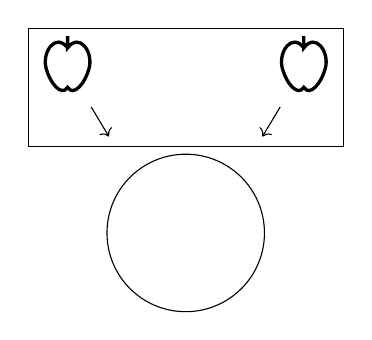
\begin{tikzpicture}
\draw (0,0) -- (4,0) -- (4,1.5) -- (0,1.5) -- cycle; 
\pic[draw, very thick, scale=.25] at (.5,1) {apple};
\pic[draw, very thick, scale=.25] at (3.5,1) {apple};
\draw[->] (.8, 0.5) -- (1.025,.125);
\draw[->] (3.2, 0.5) -- (2.975,.125);
\draw (2,-1.1) circle (1);
\end{tikzpicture}

In general iff no nonuniformities of $\Phi$ can be detected.

\section{Strong equivalence principle}
Object only feels result of curvature from \undline{other objects}.
\remark{self-interaction strongly limited}
\begin{eigenschap}
General relativity is uniquely compatible with the strong equivalence principle.
\end{eigenschap}

\section{Experimental evidence}
\subsection{Eötvös experiment}
[Insert picture here]
Eötvös parameter:
\[ \eta = 2 \frac{a_2-a_1}{a_2+a_1} = \frac{\left(\frac{m_g}{m_I}\right)_2 - \left(\frac{m_g}{m_I}\right)_1}{\left(\frac{m_g}{m_I}\right)_2 + \left(\frac{m_g}{m_I}\right)_1} \]
With the following results:
\begin{align*}
\eta_{\text{Be},\text{T}} &= (0,3 \pm 1,8)\cdot 10^{-13} \\
\eta_{\text{Be},\text{Al}} &= (-0,7 \pm 1,3)\cdot 10^{-13} \\
\eta_{\text{Earth},\text{Moon}} &= (\quad \pm \quad)\cdot 10^{} \\
\end{align*}

\subsection{MICROSCOPE}
MICRO-Satellite à traînée Compensée pour l'Observation du Principe d'Equivalence (MICROSCOPE). Tests WEP up to $10^{-15}$.
\[ \eta < 2,1\times 10^{-14} \]

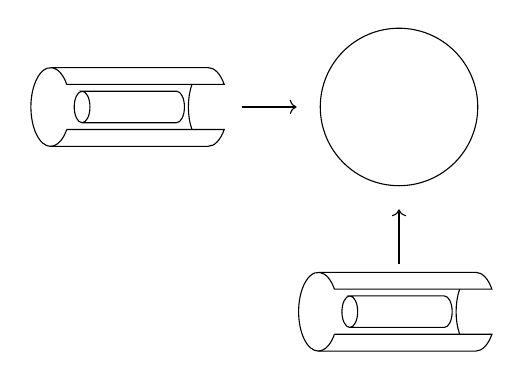
\begin{tikzpicture}[microscope/.pic={
\path (0,0) -- ++(-1.55,0) arc (0:360-35:.5 and 1) coordinate (start);
\path (start)  arc (360-35:90:.5 and 1) coordinate (p1);
\path (start)  arc (360-35:270:.5 and 1) coordinate (p2);
\draw (start) arc (360-35:35:.5 and 1) -- ++(4,0) arc (35:90:.5 and 1) -- (p1);
\draw (start) -- ++(4,0) arc (360-35:360-90:.5 and 1) -- (p2);
\path (start) -- ++(4,0)  arc (360-35:180+35:.5 and 1) coordinate (p3);
\draw (p3) arc (180+35:180-35:.5 and 1);
\path (start) arc (360-35:0:.5 and 1) -- ++ (.5,0) arc (0:90:.2 and .4) coordinate (c2);
\draw (c2) arc (90:360+90:.2 and .4) -- ++(2.4,0) arc (90:90-180:.2 and .4) -- ++(-2.4,0);
}]
\pic[draw, scale=.5] at (-3.4,0) {microscope};
\pic[draw, scale=.5] at (0,-2.6) {microscope};
\draw[->] (-2,0) -- (-1.3,0);
\draw[->] (0,-2) -- (0,-1.3);
\draw (0,0) circle (1);
\end{tikzpicture}

\section{Towards general covariance}
\subsection{Newtonian gravity in spacetime terms}
6.6 Hartle
\[ \diff{s}^2 = - \left(1+ \frac{2\Phi(x^i)}{c^2}\right)(c \diff{t})^2 + \left(1- \frac{2\Phi(x^i)}{c^2}\right)(\diff{x}^2 + \diff{y}^2 + \diff{z}^2) \]
Static weak field approximation


\chapter{Consequences of the equivalence principles and overview of general relativity}
In this section we explore some of the consequences of the equivalence principles. Then we give a very quick overview of way we will be building up the theory of general relativity in this section. This should hopefully serve to justify the somewhat involved mathematics of the next section.

\section{Gravitational redshift}
\[ \omega_\infty = \left(1- \frac{G_N M}{Rc^2}\right)\omega_* \]

\section{Geometric interpretation of gravity}
spacetime: differentiable manifold
Chapt 6.5 Hartle

Gravity as a property of space, so we need to review how we see space. We need it to be approximately flat in small areas. This idea is captured in the rigourous, mathematical notion of a manifold.

We take spacetime to be a differentiable manifold, meaning we can still do calculus to points in the manifold.

We also still want to be able to use vectors, and in general tensors, on the manifold. Here we run into a slight problem: vectors in different points are incompatible with each other. Concepts such as the displacement and position vector only work in flat space. Instead we construct a vector space (and more generally tensors) in each point. That vector space is called the tangent space in a point. (TODO Why + link to curvature)

We can however link the tangent spaces in neighbouring points using connections. These are not inherent in a manifold and specify the curvature. There is another (more intuitive) way to specify the curvature: using a metric. Here our concept of metric will be slightly different (!) than when we discussed metric spaces above. A major difference will be that we will not require it to be positive definite.

\section{Causality}



\section{Rindler spacetime}
\subsection{Uniformly accelerated observers}
\[ \diff{s}^2 = - \diff{t}^2 + \diff{x}^2 \]
We study uniformly accelerating object (indestiguishable from gravity in local experiments):
\[ \alpha^2 = \alpha^\mu\alpha_\mu = a^2 \qquad x(0) = \frac{1}{a} \]
With $\alpha$ the acceleration.
Following is basic SR kinematics
\[x(t) = x(0) + \frac{1}{a} \sqrt{1+a^2t^2}- \frac{1}{a} = \frac{1}{a} \sqrt{1+a^2t^2}\]
\[ \begin{cases}
t(\tau) = \frac{1}{a} \sinh(a\tau) \\
x(\tau) = \frac{1}{a} \sqrt{1+\sinh^2(a\tau)}
\end{cases} \qquad x^\mu(\tau) = \frac{1}{a} \begin{pmatrix}
\sinh(a\tau) \\ \cosh(a\tau)
\end{pmatrix}\]

%See drawing
[Note to self: look up Minkowski diagram]

Still compatible with assumptions:
\[ u^\mu = \od{x^\mu}{\tau} = \begin{pmatrix}
\cosh(a\tau) \\ \sinh(a\tau)
\end{pmatrix} \qquad \alpha^\mu \od[2]{x^\mu}{\tau} = a \begin{pmatrix}
\sinh(a\tau) \\ \cosh(a\tau)
\end{pmatrix} \]
\[\alpha^\mu\alpha_\mu = a^2 (-\sinh^2(a\tau)+\cosh^2(a\tau)) = a^2\]

\subsection{Adapted coordinates}
Change variables so that $\xi = 0$ gives trajectory of object.
\[ \begin{pmatrix}
t \\ x
\end{pmatrix} \mapsto \begin{pmatrix}
\tau \\ \xi
\end{pmatrix} \]
A t = 0 both observers have same spacetime

Change of coordinates is singular: can only describe part of spacetime.

\[ \begin{cases}
t (\tau, \xi = 0) = \frac{1}{a} \sinh(a\tau) \\
x(\tau, \xi = 0) = \frac{1}{a} \cosh(a\tau)
\end{cases}\]
\[ x(\tau = 0, \xi) = \frac{f(\xi)}{a} ?? \]

We want $x = 0$ is $\xi = -\infty$, so $\log$, because $x=0$ will be singular:
\[ x \in ]0,+\infty[, t \in \R \to \xi \in \R, \tau \in \R \]
So we choose:
\[ \begin{cases}
t (\tau, \xi) = \frac{e^{a\xi}}{a} \sinh(a\tau) \\
x(\tau, \xi) = \frac{ e^{a\xi} }{a} \cosh(a\tau)
\end{cases}\]
\[ \begin{cases}
\tau(t,x) = \frac{1}{a} \atanh(t/x) \\
\xi(t,x) = \frac{1}{2a} \log[a^2(x^2 - t^2)]
\end{cases} \]
Argument of $\log$ has to be positive, so only describes wedge, not even light cone.

\[ \diff{s}^2 = - \diff{t}^2 + \diff{x}^2 \]
\begin{align*} \diff{s}^2 &= -\left(\pd{t}{\xi} \diff{\xi} + \pd{t}{\tau} \diff{\tau}\right)^2+\left( \pd{x}{\xi} \diff{\xi} + \pd{x}{\tau} \diff{\tau} \right)^2 \\
=& -(e^{a\xi}\sinh(a\tau)\diff{\xi} + e^{a\xi}\cosh(a\tau)\diff{\tau})^2
+(e^{a\xi}\cosh(a\tau)\diff{\xi} + e^{a\xi}\sinh(a\tau)\diff{\tau})^2
=& e^{2a\xi}
\end{align*}

\[ \diff{s}^2 = - \diff{t}^2 + \diff{x}^2 = e^{2a\xi}(- \diff{\tau}^2 + \diff{\xi}^2)\]

\subsection{Rindler spacetime (time dilation, event horizons)}

Now take observer at $\xi = 0$, so $t = \frac{1}{a}\sinh(a\tau)$ and $x = \frac{1}{a} \cosh(a\tau)$. Then observe $\xi = 1$:
\[ \begin{cases}
t = \frac{e^{a}}{a} \sinh(a\tau) = \frac{1}{a'} \sinh(a'\tau') \qquad a'=ae^{-a} < a\\
x = \frac{e^{a}}{a} \cosh(a\tau) = \frac{1}{a'} \cosh(a'\tau') \qquad \tau' = \frac{a}{a'} \tau = e^{a}\tau > \tau
\end{cases} \]
Less acceleration means time flows faster, more acceleration means time flows slower.

Now for $\xi = -1$:
\[ \begin{cases}
t = \frac{e^{-a}}{a} \sinh(a\tau) = \frac{1}{a''} \sinh(a''\tau'') \qquad a''=ae^{a} > a\\
x = \frac{e^{-a}}{a} \cosh(a\tau) = \frac{1}{a''} \cosh(a''\tau'') \qquad \tau'' = \frac{a}{a''} \tau = e^{-a}\tau < \tau
\end{cases} \]

Clock in satellite: two competing effects.

Redshift: $\sqrt{-g_{\tau\tau}} = \sqrt{e^{2a\xi}} = e^{a\xi}$


Even if metric is singular, the space is not singular! (Extend I to II, and then to IV)

\[ g_{\mu\nu} = \begin{pmatrix}
-e^{2a\xi} & 0 \\
0& e^{2a\xi}
\end{pmatrix} \qquad \partial_{\tau}g_{\mu\nu} = 0 \]

\[u^{\mu} = \begin{pmatrix}
1\\ 0
\end{pmatrix} \qquad u = \partial_\tau\]

\begin{align*}
u^\mu u_\mu &= g_{\tau\tau} = -e^{2a\xi} < 0 \\
&= a^2(t^2-x^2)
\end{align*}
$u$ is timelike in I as it should be, but can also be lightlike or spacelike in different sections.





\chapter{Explaining the geometry of gravity: Einstein's equations}
\section{The Einstein-Hilbert action}
\section{Einstein's equations}
\section{The stress-energy tensor}
(stress tensor for a gas of particles)

\section{Couplings to other fields}

\[x^\mu : \R \to \R^{1,3}: \tau \mapsto \]

% See notes

Now we describe free motion of massive particle. The action is:
\[ S[x^\mu(\tau)] = -m\int \diff{s} \]
Describe for arbitrary metric
\[\diff{s}^2 = \diff{x}^\mu \diff{x}^\nu g_{\mu\nu}(x)\]
Extremise $S$! Trajectory of massive particle given by maximum. (Massless more difficult).
\[\delta S = -m\int \delta\left(\sqrt{-\dot{x}^\mu\dot{x}^\nu g_{\mu\nu}(x)}\right)\diff{\tau} = m \int \frac{1}{2\sqrt{-\dot{x}^2}}\left(2\dot{x}^\mu \od{\delta x^\nu}{\tau} g_{\mu\nu} + \dot{x}^\mu\dot{x}^\nu \pd{g_{\mu\nu}}{x^\rho}\delta x^\rho\right) \diff{\tau}\]
Using that $\dot{x}^2$ is constant, this is equal to
\[ m\int \frac{1}{2\sqrt{-\dot{x}^2}}\left(\ddot{x}^\mu g_{\mu\nu} \delta x^\nu - \dot{x}^\mu \delta x^\nu \pd{g_{\mu\nu}}{x^\rho}\dot{x}^\rho + \frac{1}{2} \dot{x}^\mu \dot{x}^\nu \pd{g_{\mu\nu}}{x^\rho} \delta x^\rho\right) \diff{\tau} = 0\]
\begin{align*} \delta S &= -m \int \frac{1}{2\sqrt{-\dot{x}^2}}\left(\ddot{x}^\mu g_{\mu\rho} + \dot{x}^\mu \dot{x}^\nu \partial_\nu g_{\mu\rho} - \frac{1}{2} \dot{x}^\mu \dot{x}^\nu \partial_\rho g_{\mu\rho}\right)\delta x^\rho \diff{\tau} \\
&= -m \int \frac{g_{\mu\rho}}{2\sqrt{-\dot{x}^2}}\left(\ddot{x}^\mu + g^{\mu\sigma} \partial_\tau g_{\mu\rho} \dot{x}^\nu \dot{x}^\tau - \frac{1}{2}g^{\mu\sigma}\partial_\sigma g_{\mu\tau}\dot{x}^\nu \dot{x}^\tau\right)\delta x^\rho \diff{\tau}
\end{align*}

\[ \delta S = -m \int \frac{g_{\mu\rho}}{2\sqrt{-\dot{x}^2}} \frac{D\dot{x}^\mu}{D\tau} \delta x^\rho \diff{\tau}\]
\[ \frac{D\dot{x}^\mu}{D\tau} =  \od[2]{x^\mu}{\tau} + \frac{1}{2} g^{\mu\sigma} \left(\partial_\nu g_{\rho\sigma} + \partial_\rho g_{\nu\sigma} - \partial_\sigma g_{\nu\rho}\right)\dot{x}^{\nu}\dot{x}^\rho = 0\]
Christoffel symbols
\[ \Gamma^\mu_{\nu\rho} \equiv \frac{1}{2} g^{\mu\sigma} \left(\partial_\nu g_{\rho\sigma} + \partial_\rho g_{\nu\sigma} - \partial_\sigma g_{\nu\rho}\right)\]
What about partical with other parameter than $\tau$? Or massless particles?
We want a procedure that is reparametrisation invariant.
Change of coordinates that is never singular:
\[ \tau \to \tau'= \tau'(\tau) \qquad \od{\tau'}{\tau} \neq 0 \qquad \diff{s}^2 = \diff{x}^\mu \diff{x}^\nu g_{\mu\nu}(x)\]
\[ \diff{s}^2 = \diff{\tau}^2\gamma_{\tau\tau}(\tau) = \diff{\tau'}\diff{\tau'}\gamma_{\tau'\tau'} = \diff{\tau'}\diff{\tau'}\od{\tau}{\tau'}\od{\tau}{\tau'}\gamma_{\tau\tau}\]
\[ \gamma_{\tau'\tau'} = \left(\od{\tau}{\tau'} \right)^2\gamma_{\tau\tau} \]
\[ \gamma_{\tau\tau} = \left(\od{\tau}{\tau'} \right)^2\gamma_{\tau'\tau'} \]
Proper time: $\gamma_{\tau\tau} = -1$
Polyakov's action:
\[ S = - \frac{1}{2} \diff{\tau} \sqrt{\gamma} \left[ \gamma^{\tau\tau} \od{x^\mu}{\tau} \od{x^\nu}{\tau} g_{\mu\nu}(x) + m^2 \right] \]
($\tau$ generic parameter)

We can also describe motion of particle, string or brane:
\begin{itemize}
\item 0-dim object $\to$ 1-dim worldline
\item 1-dim object $\to$ 2-dim worldsheet
\end{itemize}

Write action in terms of $e$ ($\gamma_{\tau\tau}(\tau) = -e^2(\tau)$)
\[ S[x^\mu,e] = \frac{1}{2} \int \diff{\tau} [e^{-1}\dot{x}^\mu\dot{x}^\nu g_{\mu\nu} - em^2] \]
\begin{align*} \frac{\delta S}{\partial x^\mu} &\sim e^{-1}[2\dot{x}^\mu \delta \dot{x}^\nu g_{\mu\nu} + \dot{x}^\mu\dot{x}^\nu \partial_\rho g_{\mu\nu} \delta x^\rho] \\ &= \int \diff{\tau}e^{-1} \left[ - \frac{D\dot{x}^\mu}{D\tau} g_{\mu\nu} \delta x^\nu \right] = 0 \end{align*}
For massless particle: simply put $m=0$

\[ \pd{S}{e} \sim -e^{-2}\dot{x}^2 - m^2 = 0 \]
\remark{$m=0$ particle: $\dot{x}^2 = 0$}
\remark{for $m\neq 0$: $e^2 = \frac{m^2}{-\dot{x}^2} \qquad e = \frac{m}{\sqrt{-\dot{x}^2}}$}

Equation of motion (?):
\[ \frac{D\dot{x}^\mu}{\tau} = 0 =	\od[2]{x^\mu}{\tau} + \Gamma^\mu_{\nu\rho}\od{x^\nu}{\tau}\od{x^\rho}{\tau} = 0 \]
Using the following
\[\sigma = f(\tau): \qquad \od{}{\tau} = \od{f}{\tau}\od{}{\sigma} \qquad \od[2]{}{\tau} = \ddot{f}\od{}{\sigma} + (\dot{f}^2)\od[0]{}{\sigma}\]
we get
\[ \ddot{f}\od{x^\mu}{\sigma} + \dot{f}^2 \od[2]{x^\mu}{\sigma} + \Gamma^\mu_{\nu\rho}\od{x^\nu}{\sigma} \od{x^\rho}{\sigma}(\dot{f})^2 = 0  \]

Lecture 18/10

Polyakov's action ($\diff{s}^2|_{\text{on woldline}} = - e(\tau)^2 \diff{\tau}$)
\[ S= \frac{1}{2} \int \diff{\tau}(e^{-1}\dot{x}^2 - em^2) \]
\[ \delta_e S = - \frac{1}{2}\int \diff{\tau}(+e^{-2}\dot{x}^2 + m^2)\delta e \]
\begin{align*} \delta_x S &= \frac{1}{2}\int \diff{\tau}(2e^{-1}\dot{x}^\mu g_{\mu\nu} \od{\delta x}{\tau} + e^{-1}\dot{x}^\mu \dot{x}^\rho \partial_\nu g_{\mu\rho}\delta x^\nu) \\
&= \int \diff{\tau}e^{-1}(\frac{D \dot{x}^\mu}{\tau}g_{\mu\nu}\delta x + e^{-2} \od{e}{\tau} \dot{x}^\mu g_{\mu\rho}\delta x^\nu)
\end{align*}

Where
\[ \frac{D \dot{x}^\mu}{\tau} \equiv = \od{\dot{x}}{\tau} + \Gamma^\mu_{\nu\rho}\dot{x}^\nu\dot{x}^\rho \]
with $\Gamma^\mu_{\nu\rho} = \frac{1}{2}$. We use the following notation:
\[ \begin{cases}
(\mu\nu) = \frac{1}{2} (\mu\nu + F_\nu\mu)
[\mu\nu] = \frac{1}{2} (\mu\nu - F_\nu\mu)
\end{cases} \]
For example with EM tensor $F$: $F_{[\mu\nu]} = \frac{1}{2}(F_{\mu\nu - F_\nu\mu}) = 0$ (F antisymm).

Now this:
\[ g_{00} = -(1+2 \frac{V(\vec{x})}{m}) \qquad g_{ij} = \delta_{ij} \]
Using $\frac{V}{m}$
\begin{align*}
S = -m \int \sqrt{(1+\frac{2V}{m})- \left|\od{\vec{x}}{t} \right|} \od{t}{\tau} \diff{\tau} \\
&\approx -m \int (1+\frac{V}{m}- \frac{1}{2}\left|\vec{x}\right|^2) \diff{t} \\
&= -m \int \diff{t} + \int \left[\frac{1}{2}m \left|\vec{x}\right|^2 - V(\vec{x})\right] \diff{t}
\end{align*}
In worldline (1D?) ($\gamma:\tau \mapsto x^\mu(\tau)$)
\[ S_1 = q \int_\gamma \diff{x}^\mu A_\mu(x) \]
\[ \delta A_\mu = \partial_\mu = \partial_\mu \Lambda \overset{\text{gauge invariance}}{\to}  \delta_\Lambda S_1 = q \int_\gamma \diff{x}^\mu \partial_\mu \Lambda \]
\begin{align*}
\delta_xS_1 &= q \int_\gamma \diff{\delta x^\mu} A_{\mu} + q \int_{\gamma} \diff{x}^\mu \partial_\nu A_\mu \delta x^\nu \\
&= q \int_\gamma \left[ \od{\delta x^\mu}{\tau}  A_{\mu} + \od{{x}^\mu}{\tau} \partial_\nu A_\mu \delta x^\nu \right] \diff{t} \\
&= q \left[ -\delta x^\mu \partial_\nu  A_{\mu} \dot{x}^\nu + \dot{x}^\nu \partial_\nu A_\mu \delta x^\nu \right] \diff{t} \\
&= -q \int F_{\mu\nu} \dot{x}^\mu \diff{x^\nu}\diff{\tau}
\end{align*}

\[ \frac{D \dot{x}^\mu}{\tau} = \frac{q}{m}F^{\mu\nu} \]


\chapter{Symmetries and simplifications}

\chapter{Some physics of gravitation}
\section{Weak field approximation}
\section{Gravitational redshift (GPS)}
Weak gravity
\[ \diff{s}^2 = - \left(1+2\phi\right)\diff{t}^2 + \delta_{ij}\diff{x}^i \diff{x}^j \]
Earth: $\phi = -G_N \frac{M_\oplus}{r}$
[picture with satellites]
Two competing effects: satellites going faster but also in weaker gravity.
\[ \frac{\nu_{s\to e}}{\nu_s} = \frac{\nu_{s\to e}}{\nu_e} = \sqrt{\frac{g_{\mu\nu}(r_s)\od{x^\mu}{t}\od{x^\nu}{t}}{g_{00}(r_e)}} = \sqrt{\frac{1+2\phi(r_s)-v_s^2}{1+2\phi(r_e)}} \]
Using $v_s^2 = G \frac{M_\oplus}{R_\oplus+h}$ and $\phi(r_s = R_\oplus + h) = - \frac{GM_\oplus}{R_\oplus + h}$, we get
\[ = \sqrt{\frac{1-3G \frac{M_\oplus}{R_\oplus + h}}{1-2G \frac{M_\oplus}{R_\oplus}}} \approx 1 - \frac{3}{2} G \frac{M_\oplus}{R_\oplus + h} + G \frac{M_\oplus}{R_\oplus} \]
\[ = ???? missed \]
Sometimes redshift, sometimes blueshift. (Missed calculation of when)
\section{Gravity waves}
Small, time dependent perturbations
\[ g_{\mu\nu} = \eta_{\mu\nu} + h_{\mu\nu} \]
Where $\left|h\right|\sim 10^{-21}$??
Not produced in big quantities (we do not see effects in cosmic microwave background radiation)
Indirect detection: period of pulsars (like PSR 1913+16). They collapse because they lose (radiate) energy as gravitational waves. Also direct observation.

CFR. EM
\[ \begin{cases}
\diff{F} = 0 \\ \diff{*F} = 0
\end{cases} \qquad \to \qquad \Box A^\mu - \partial^\mu\partial_\nu A^\nu = 0 \]
\[ \begin{cases}
\Box A^\mu = 0 \\ \partial_\mu A^\mu = 0 \qquad \text{gauge}
\end{cases} \]
\[ A^\mu = c^\mu e^{-ik_\mu x^\mu} \]
\[ k^2 = 0 \qquad k_\mu c^\mu = 0 \qquad A^\mu = ak^\mu + \tilde{c}^\mu \]
\[ k^\mu = |k| \begin{pmatrix}
1\\0\\0\\1
\end{pmatrix} \qquad \tilde{c}^\mu = \begin{pmatrix}
0\\ \tilde{c}^1 \\ \tilde{c}^2 \\ 0
\end{pmatrix} \]


We want to do the same with $R_{\mu\nu} = 0$. In order to do that we need to linearize
\[ R_{\mu\nu}(h) = 0 \]
We raise and lower indices with $\eta$ because rest is of order $h^2$.
\[ g^{\mu\nu} = \eta^{\mu\nu} - h^{\mu\nu} \]
\[ h^{\mu\nu} = \eta^{\mu\rho}\eta^{\nu\sigma}h_{\rho\sigma} \]
\[\Gamma^\mu_{\nu\rho}(h) = \frac{1}{2}\eta^{\mu\sigma}\left(\partial_\nu h_{\rho\sigma} + \partial_\rho h_{\nu\sigma} - \partial_\sigma h_{\rho\nu}\right)\]

\begin{align*}
R_{\mu\nu}(h) &= R_{\alpha\mu\;\nu}^{\;\;\alpha}(h) = \partial_\alpha\Gamma^\alpha_{\mu\nu} - \partial_\mu\Gamma^\alpha_{\alpha\nu} \\
&= \frac{1}{2}\left[\eta^{\alpha\sigma}\partial_\alpha \left(\partial_\mu h_{\nu\sigma}+\partial_\nu h_{\mu\sigma}-\partial_\sigma h_{\mu\nu}\right)- \eta^{\alpha\sigma}\partial_\mu \left(\partial_\alpha h_{\nu\sigma}+\partial_\nu h_{\alpha\sigma}-\partial_\sigma h_{\alpha\nu}\right)\right]
\end{align*}

\[ R_{\mu\nu}(h) = \frac{1}{2} \left[\partial^\mu\partial^\sigma h_{\nu\sigma} + \partial_\nu\partial^\sigma h_{\mu\sigma} - \Box_\eta h_{\mu\nu} - \partial_\mu\partial^\sigma h_{\nu\sigma} - \partial_\mu\partial_\nu h + \partial_\mu\partial^\sigma h_{\nu\sigma}\right] = 0 \]
\[ \boxed{\Box h_{\mu\nu} + \partial_\mu\partial\nu h - \partial_\nu\partial^\sigma h_{\nu\sigma} - \partial_\nu\partial^\sigma h_{\mu\sigma} = 0} \]
Now we need to fix invariance under diffeomorphism. How many functions an we use? In EM we can fix one.

Missed bunch ($h$ is trace)

deDonder gauge
\[ \boxed{\Gamma^\rho_{\mu\nu}g^{\mu\nu} = 0} \]

Again missed a bunch

\[ \boxed{\partial^\mu h_{\mu\nu} - \frac{1}{2}\partial_\nu h = 0} \qquad \text{gauge} \]

So we have:
From Einstein ($R_{\mu\nu}(h) = 0$) and the deDonder gauge ($\Gamma^\rho_{\mu\nu}g^{\mu\nu} = 0$) we get
\[ \begin{cases}
\Box h_{\mu\nu} = 0 \\ \partial^\mu h_{\mu\nu} - \frac{1}{2}\partial_\nu h = 0
\end{cases} \]
$\Box h_{\mu\nu} = 0$ implies $\Box h = 0$. To put it in a better form we call
\[ \bar{h}_{\mu\nu} \equiv h_{\mu\nu} - \frac{1}{2}\eta_{\mu\nu} h \]
for the trace we have
\[ \bar{h} = h - \frac{1}{2}4h = -h \]
We then get 
\[ \begin{cases}
\Box\bar{h}_{\mu\nu} = 0 \\ \partial^\mu \bar{h}_{\mu\nu} = 0
\end{cases} \]

\[ c_{\mu\nu} = \begin{pmatrix}
c_{00}&c_{01}&c_{02}&-c_{00} \\
c_{01}&c_{11}&c_{12}&-c_{10} \\
c_{02}&c_{12}&c_{22}&-c_{20} \\
-c_{10}&-c_{10}&-c_{20}&+c_{00} \\
\end{pmatrix} \]

\[\bar{h}_{\mu\nu} = c_{\mu\nu}e^{-ik_\rho x^\rho}, \qquad k^2 =0, \qquad k^\mu c_{\mu\nu}\]
\[ k^\mu = \begin{pmatrix}
1\\0\\0\\1
\end{pmatrix} \qquad c_{0\nu}+c_{3\nu} = 0 \]
\begin{align*}
\delta h_{\mu\nu} &= \partial_\mu \epsilon_\nu + \partial_\nu\epsilon_\mu \\
\delta h_{\mu\nu} &= \partial_\mu \epsilon_\nu + \partial_\nu\epsilon_\mu - \partial^\rho\epsilon_\rho\eta_{\mu\nu} \\
\delta c_{\mu\nu} &= k_\mu \epsilon_\nu + k_\nu\epsilon_\mu - k^\rho\epsilon_\rho\eta_{\mu\nu} \\
\end{align*}
so
\begin{align*}
&\delta c_{00} = -2\epsilon_0+ (\epsilon_0+\epsilon_3) = \epsilon_3-\epsilon_0 \\
&\delta c_{01} = -\epsilon_1 \\
&\delta c_{02} = -\epsilon_2 \\
&\delta c_{12} = 0 \\
&\delta c_{11} = -(\epsilon_0+\epsilon_3) \\
&\delta c_{22} = -(\epsilon_0+\epsilon_3) \\
\end{align*}

We finally get the transverse traceless polarization vector
\[c_{\mu\nu} = \begin{pmatrix}
0 &0&0&0 \\
0&c_{11}&c_{12} & 0\\
0&c_{12}&-c_{11}&0 \\
0 &0&0&0 \\
\end{pmatrix}\]

\[ \diff{s}^2 = - \diff{t}^2 + \diff{z}^2 + \diff{x}^2(1+c_{11}\cos(t+z))+\diff{y}^2(1-c_{11}\cos(t-z)) \]
\[ c_{11}, c_{12} \sim 10^{-21} \]

Missed several lectures??

Lecture 22/11
(Approx size of $c_{11}$??)

\subsection{Gravity waves: detection}
\[ \diff{s}^2 =  - \diff{t}^2 + \diff{z}^2 + \diff{x}^2(1+c_{11}\cos \alpha or \kappa (t-z)) + \diff{y}^2(1+c_{11}\cos \alpha or \kappa (t-z)) + 2 \diff{x} \diff{y} c_{12}\cos \alpha or \kappa (t-z)\]
Geodesic detection equation
\[ \od[2]{x(t)}{t} = -\delta^i\partial_i \phi(x(t)) \qquad x^i(t) = x_*^i(t) + \chi^i(t) \]
\[ \od[2]{x^i_*(t)}{t} + \od[2]{\chi^i(t)}{t} = -\delta^{ij}\partial_j\phi(x^*(t)) - \delta^{ij}\partial_\kappa\partial_j\phi(x^*(t))\chi^*(t) + \mathcal{O}(\chi^2) \]
So
\[ \od[2]{\chi^i(t)}{t} \approx - \delta^{ij}\underbrace{\partial_\kappa\partial_j\phi(x^*(t))}_{\text{tidal tensor}}\chi^*(t) \]

How does difference between $x^\mu(\tau_x)$ and $y^\mu(\tau_y)$ change with time? (We set $\tau=\tau_x=\tau_y$). $\epsilon^\mu(\tau_x,\tau_y) = x^\mu(\tau_x) - y^\mu(\tau_y)$


Simplified calculation with special reference frame, but with covariant result. (Caroll does it fully covariantly, much longer)
Choose coordinates (Fermi normal coordinates) such that
\begin{align*}
&g_{\mu\nu}(x_*) = \eta_{\mu\nu} \\
&\partial_\rho g_{\mu\nu}(x_*) = 0 = \Gamma_{\nu\rho}^\mu(x^*) \\
&g_{\mu\nu}(x_*) = \eta_{\mu\nu} + \mathcal{O}(|x-x^*|^2)\\
&\partial_\rho g_{\mu\nu}(x(t)) = 0 = \Gamma_{\nu\rho}^\mu(x(t)) \\
\end{align*}
is satisfied along geodesic! (Is possible, proved by Fermi)

\[ \ddot{y}^\mu + \Gamma^\mu_{\nu\rho}(y(\tau))\dot{y}^\nu \dot{y}^\rho = 0 \]
We compute $\epsilon$
\begin{align*}
\ddot{\epsilon}^\mu &= \ddot{y}^\mu - \ddot{x}^\mu \\
&= -\Gamma^\mu_{\nu\rho}(y) \dot{y}^\nu \dot{y}^\rho \\
&= ???????
\end{align*}
\[ y^\mu(\tau) = x^\mu(\tau) + \epsilon^\mu(\tau) \]
\[ \ddot{\epsilon}^\mu = -\epsilon^\sigma\partial_\sigma\Gamma^\mu_{\nu\rho}(x)\dot{x}^\nu \dot{x}^\rho \qquad \text{first order in $\epsilon$}\]

\begin{align*}
\frac{D^2 \epsilon^\mu}{D \tau} &= \frac{D}{D\tau}\left[\frac{D\epsilon^\mu}{D\tau}\right] = \frac{D}{D\tau}\left(\dot{\epsilon}^\mu+\Gamma^\mu_{\nu\rho}(x)\epsilon^\nu \dot{x}^\rho\right) \\
&= \ddot{\epsilon}^\mu + \od{}{\tau}\left(\Gamma^\mu_{\nu\rho}(x)\epsilon^\nu\dot{x}^\rho\right) + \cancel{\Gamma^\mu_{\nu\rho}(x)\frac{D\epsilon^\nu}{D\tau}\dot{x}^\rho} \\
&= \ddot{\epsilon}^\mu + \dot{x}^\sigma\partial_\sigma\Gamma^\mu_{\nu\rho}(x)\epsilon^\nu\dot{x}^\rho \\
&= -\epsilon^\sigma\partial_\sigma\Gamma^\mu_{\nu\rho}\dot(x)^\nu\dot{x}^\rho + \dot{x}^\sigma\partial_\sigma\Gamma^\mu_{\nu\rho}\epsilon^\nu\dot{x}^\rho \\
&= \epsilon^\sigma\dot{x}^\nu\dot{x}^\rho \left(-\partial_\sigma\Gamma^\mu_{\nu\rho}(x) + \partial_\nu\Gamma^\mu_{\sigma\rho}(x)\right) = - R_{\sigma\nu\;\rho}^{\;\;\mu}\epsilon^\sigma\dot{x}^\nu\dot{x}^\rho
\end{align*}
\[ \boxed{\frac{D^2\epsilon^\mu}{D\tau^2} = - R_{\sigma\nu\;\rho}^{\;\;\mu}\epsilon^\sigma\dot{x}^\nu\dot{x}^\rho} \]

Now we use this metric
\[ \diff{s}^2 =  - \diff{t}^2 + \diff{z}^2 + \diff{x}^2(1+c_{11}\cos\kappa(t-z)) + \diff{y}^2(1+c_{11}\cos\kappa(t-z)) + 2 \diff{x} \diff{y} c_{12}\cos\kappa(t-z)\]
geodesic doesn't change ?!? But proper distance changes.

\[ g_{\mu\nu} = \eta_{\mu\nu} + h_{\mu\nu} \qquad h_{00}=h_{0i} = h_{zz} = h_{z0} = h_{zi} = 0\]
\[ h_{ij} \qquad i,j = x,y \]
\[ \begin{cases}
\dot{x}^0 = 1 =\dot{y}^0 \\
\dot{x}^{i,z} = 0 = \dot{y}^{i,z}
\end{cases}\qquad \begin{pmatrix}
1\\0\\0\\0
\end{pmatrix} \]

\[ \od[2]{\epsilon^\mu}{t} = -R_{\sigma0\;0}^{\;\;\mu}\epsilon^\sigma \]
\begin{align*}
\od[2]{\epsilon^i}{t}&= -R_{j0\;0}^{\;\;i}\epsilon^j \\
&= - \left(\partial_j\Gamma_{00}^i - \partial_0\Gamma^i_{j0}\right)\epsilon^j
\end{align*}

\[ \od[2]{\epsilon^i}{t} = + \partial_0\Gamma^i_{j0}\epsilon^j = \frac{1}{2}\delta^{ik}\left(\od[2]{}{t}h_{kj}\right)\epsilon^j \]
\[ \begin{cases}
\ddot{\epsilon}^x = - \frac{1}{2}c_{11} \cos(\kappa t)\epsilon^x \\
\ddot{\epsilon}^y = + \frac{1}{2}c_{11} \cos(\kappa t)\epsilon^y \\
\end{cases} \]
\[ \begin{cases}
\epsilon^x(t) = \left(1+ \frac{1}{2}c_{11}\cos(\kappa t)\right)\epsilon^x(0) + \mathcal{O}(c_11^2) \\
\epsilon^y(t) = \left(1- \frac{1}{2}c_{11}\cos(\kappa t)\right)\epsilon^y(0) + \mathcal{O}(c_11^2) \\
\end{cases} \]

If quantizable, gravity has spin 2. A theorem states that particles of spin more than 2 are completely decoupled. What about 3/2?
Squishing and stretching of circle [picture]
\section{Physical effects of gravity waves (geodesic deviation equation)}

\chapter{Gravity outside a spherical mass: Schwarzschild's solution}
\section{Solving Einstein's equations using symmetries}
Solve Einstein equtions. Solve for $R_{\mu\nu} = 0$.

We assume spherical symmetry, so we have 3 Killing vectors.
\[ [K_I, K_S] = \epsilon_{IJK}K_K \qquad I,J = 1,2,3 \]
\[ K_I = K_I^\mu\partial_\mu \qquad D_{[\mu}K_{I\nu]} = 0  \]
We also assume static spacetime ($\neq$ stationary). This assumption is not necessary to reach Schwarzschild, but helps.
\[ \diff{s}^2 = g_{00}\diff{t}^2 + g_{0i}\diff{t}\diff{x}^i + g_{ij}\diff{x}^i \diff{x}^j \]
Stationary means you can foliate space layers [fig].
\[ \exists \xi_t = \xi_t^\mu\partial_\mu, \qquad \xi_t^2 < 0 \qquad D_{[\mu}\xi_{t\nu]} = 0 \]
\[ \Leftrightarrow \xi_t^\mu\partial_\mu g_{\nu\rho} + g_{\mu\nu}\partial_\rho\xi^\mu_t + g_{\mu\rho}\partial_\nu\xi_t^\mu = 0 \]
Introduce $t$: $\xi_t = \partial_t$

Static means something more: there is no mixing of time and space coordinates(?)

\[ K_I^\mu\partial_\mu g_{\nu\rho} + g_{\mu\nu}\partial_\rho K_I^\mu + g_{\mu\rho}\partial_\nu K_I^\nu = 0 \]
\[ K_I^i\partial_i g_{00} + \cancel{2g_{i0}\partial_0K_I^i} = 0 \qquad \Rightarrow \qquad g_{00}(x) = g_{00}(r) \]
In spherical coordinates:
\[ f(r)\diff{r}^2 + g(r) \left[\diff{\theta}^2 + \sin^2\theta \diff{\phi}^2\right] \]

Ansatz for the metric:
\[ \diff{s}^2 = -A^2(r)\diff{t}^2 + B^2(r)\diff{r}^2 + C(r)^2 \left[\diff{\theta}^2 + \sin^2\theta \diff{\phi}^2\right] \]
10 equations.
``Parity invariances'':
\[ \begin{cases}
t \to -t \quad R_{tr} = 0 = R_{\theta\phi} \\
\phi \to -\phi \quad R_{t\theta} = 0 = R_{r\theta} \\
\theta \to -\theta \quad R_{t\phi} = 0 = R_{r\phi}
\end{cases} \]
So only 4 equations left.

We will use fieldbines (easier if we choose them intelligently). (Fieldbines are only defined up to a Lorentz transformation)
\[ g_{00} = -A^2 \quad g_{rr} = B^2 \quad g_{\theta\theta} = r^2 \quad g_{\phi\phi} = r^2\sin^2\theta \]
$e^a \to \omega \to \R$
\[ \diff{s}^2 = e^a\otimes e^b \eta_{ab} = -{e^0}^2 + (e^1)^2 + (e^2)^2 + (e^3)^2 \]
\[ \begin{cases}
e^0 = A(r)\diff{t} \\
e^1 = B(r)\diff{r} \\
e^2 = r \diff{\theta} \\
e^3 = r\sin\theta \diff{\phi}
\end{cases} \]
\[\diff{e^a}+\omega^a_{\;b}e^b = 0 \qquad R^a_{\;b} = \diff{\omega}^a_{\;b}+ \omega^a_{\;c}\omega^c_{\;d}\]

Missed stuff (in lecture notes)

Lecture 06/12
Ward identity for Compton scattering
\[ \mathcal{M} = -ie^2\bar{u}'\epsilon^{\prime*}_\nu\epsilon_\mu \left(\gamma^\nu \frac{\slashed{p}}{}\right) \]
[Fig see notes]
Dirac equation.

Rewrite
\begin{align*}
\epsilon_\mu\slashed{p}\gamma^\mu u = \slashed{p}\slashed{epsilon}u &= (-) ???
\end{align*}
Which gives us 
\[ \mathcal{M} = -ie^2\bar{u}' \left(\frac{\slashed{\epsilon}'\slashed{k}\slashed{\epsilon} + 2(p\cdot \epsilon)\slashed{\epsilon}^{\prime*}}{2(p\cdot k)} + \frac{-\slashed{\epsilon}\slashed{k}\slashed{\epsilon}^{\prime*} + 2(p'\cdot \epsilon)\slashed{\epsilon}^{\prime*}}{-2(p'\cdot k)}\right)u(p) \]
On-shell condition $\slashed{k}\slashed{k} = k^2 = 0$

\section{Scattering form a (``semi'' classical) external field}
No solutions satisfying simultaneously on-shellness and momentum conservation (there exist no real Minkowski moments)

Coulomb field
Semi-classicla external field.

\[ \mathcal{M} = ie\bar{u}'A_\text{ext}(\bar{q})u = ie \bar{u}'\gamma^\mu u A_{\text{ext}\mu} \]

Flux
\[ \phi = \frac{v_\text{rel}}{V} = \frac{|\bar{p}|}{VE} \]

Unpolarised x-section
\[ \od{\sigma}{\Omega'} = \frac{(2m\alpha Z)^2}{|\bar{q}|^4}\frac{1}{2}\sum_\text{spin}|\bar{u}\gamma^0u|^2 \]

\[ |\bar{\mathcal{M}}|^2 = \frac{1}{2}\Tr \left((\slashed{p}'+m)\gamma^0(\slashed{p}+m)\gamma_0\right) \]


\[ \od{\sigma}{\Omega} = \frac{(\alpha Z)^2}{4E^2v^4\sin^4 \frac{\theta}{2}}\left(1-v^2\sin^2\frac{\theta}{2}\right) \]

If $Z=1$ then hydrogen so proton charge.

Diagrams
$M\to\infty, \bar{p}_\text{proton} = \bar{0}$ 

$J_\nu$ is proton 4-current.
\[ \bar{u}_r(\bar{0})\gamma^0 u_s(\bar{0}) = \delta_{rs} \]

\[ \delta \mathcal{M} = 0 \Leftrightarrow \sum_{i\in\text{in}}Q_i - \sum_{j\in\text{out}}Q_j = 0 \]

Lecture 07/12
Missed first half: Calculation of Schwarzschild

\begin{align*} BR_{tt} + AR_{rr} &= \frac{2}{r}\frac{A'}{B^2}B + \frac{2}{r}\frac{B'}{B^2}A \\
&= \frac{2}{rB^2}\left(A'B + B'A\right) = 0
\end{align*}
\[ B=A^{-1} \qquad B' = (A^{-1})' = -A^{-2}A' \]
\[ - \frac{A'}{AB^2}+ \frac{B'}{B^3} + \left(1- \frac{1}{B^2}\right)\frac{1}{r} = -AA' - AA' + (1-A^2)\frac{1}{r} = 0 \]

\[ \diff{s}^2 = - \left(1- \frac{2m}{r}\right)\diff{t}^2 + \left(1- \frac{2m}{r}\right)^{-1}\diff{r}^2 + r^2 \left(\diff{\theta}^2 + \sin^2\theta \diff{\phi}^2\right) \]

$\R\times\SO(3)$ isometry group. 4 Killing vectors.
\section{Finding Schwarzschild}

\chapter{Physics of the solar system}
\section{Effective potential for geodesics}
\section{Geodesics for massive particles and Mercury's procession}
\section{Geodesics for massless particles}
\subsection{Bending of light rays}
\subsection{Light emitted from compact stars}
\subsection{Shapiro time delay}


Schwarschild radius
\[ r^* = 2m \]

$m$ is mass of object (compare to Kumar energy $\mathcal{E}$??)

\section{Geodesics}
\[ \mathcal{L}  = g_{\mu\nu}(x)\dot{x}^\mu \dot{x}^\nu = \epsilon \]
Where $\epsilon = \begin{cases}
0 \qquad (m=0) \\ -1 \qquad (m\neq 0)
\end{cases}$
We fill in the metric to get:
\[ \mathcal{L}  = - \left(1- \frac{2M}{r}\right)\dot{t}^2 + \left(1- \frac{2M}{r}\right)`^{-1}\dot{r}^2 + r^2 \dot{\theta}^2 + r^2\sin^2\theta\dot{\phi}^2 \]
\[Q = K_\mu\dot{x}^\mu\]
\[ \mathcal{E} = -\xi_\mu\dot{x}^\mu = -\xi^\mu g_{\mu\nu}\dot{x}^\nu = - g_{t\nu}\dot{x}^\nu = - g_{tt} \dot{t} = \left(1- \frac{2M}{r}\right)\dot{t} \]
\[ \begin{cases}
L_1 = \sin\phi\partial_\theta + \frac{\cos\phi}{\tan\theta}\partial_\phi \\
L_2 = \cos\phi\partial_\theta - \frac{\sin\phi}{\tan\theta}\partial_\phi \\
L_3 = \partial_\phi
\end{cases} \]
\[ \vec{l} = \vec{L}_\mu\dot{x}^\mu \qquad \vec{l} = \begin{pmatrix}
0\\0\\l
\end{pmatrix}\]

\[ \dot{l}(??) = \frac{\mathcal{E}}{1- \frac{2M}{r(t)}} \qquad \overset{r\to\infty}{\to} \qquad \mathcal{E} = \gamma \]

Lecture 13/12
Missed first half
?? Other stuff(?) ???

\[ m \equiv G_N \frac{M}{c^2} \]
\[ \diff{s}^2 = - \left(1- \frac{2m}{r}\right)\diff{t}^2 + \left(1- \frac{2m}{r}\right)^{-1} + r^2 \left(\diff{\theta}^2 + \sin^2\theta \diff{\phi}^2\right) \]
\[ \dot{t} = \frac{E}{1- \frac{2m}{r}} \qquad \theta = \frac{\pi}{2} \qquad \dot{\phi} = \frac{l}{r^2} \]

Extreme $\epsilon = 0 \qquad r=3m$
\[ \epsilon=-1 \qquad r_\pm = \frac{l^2}{2m}\left(1\pm\sqrt{1-r(\frac{m}{l})^2??}\right) \]

\[ \mathcal{L} _\text{eff} = \frac{\dot{r}^2}{2} + V_\text{eff}(r) = E_\text{eff} = \frac{E^2+\epsilon}{2} \]
\[ V_\text{eff} = \epsilon \frac{m}{r} + \frac{l^2}{2r^2} - \underbrace{m \frac{l^2}{r^3}}_{\text{Relativistic correction??}} \]

Massive geodesics $\epsilon = -1$
\[\od{V_\text{eff}}{r} = -\epsilon \frac{m}{r^2} - \frac{l}{r^3} + 3m \frac{l^2}{r^4} = 0 \]

second half

Escape velocity
\[ l=0 \qquad E=1 \qquad \frac{\dot{r}}{2} - \frac{m}{r} = 0 \]
\[ \dot{r} = \sqrt{\frac{2m}{r}} \qquad \overset{r\to r_s = 2m}{\to} \qquad 1 \]
With $r_s$ the Schwarzschild radius. (1 means speed of light -> no escape)

ISCO (Inner most stable circular orbit?)

Circular orbits $l \geq \sqrt{12}m$
\[ r_+ = \frac{12m^2}{2m} = 6m \]
\[ \dot{r} = ???? \]
(Energy gain massive (6\%): several times fusion process)??

Kepler's law
\[ \omega = \od{\phi}{t} = \frac{\dot{\phi}}{\dot{t}} = \frac{l}{r_+^2E}\left(1- \frac{2m}{r_+}\right) \]
$r=r_+$
\[ \frac{m}{r^2}- \frac{l^2}{r^2}\left(1-3 \frac{??}{??}??\right)??? \]
??????

Perihelion procession

\[\Delta \phi = 2\int^{r_+}_{r_-} \od{\phi}{r}\diff{r}\]
\[ \left(\od{\phi}{r}^2\right)= \frac{\dot{\phi}^2}{\dot{r}^2} = \frac{l^2}{r^4}\frac{1}{2(E_\text{eff}-V_\text{eff})} \]
\[ u = \frac{1}{r} \qquad \diff{u} = - \frac{1}{r^2}\diff{r} \]
\[ (\left(\od{r}{\phi}\right)^2)^2 = r'^2 = \frac{2r^4}{l^2}\left(E_\text{eff}-V_\text{eff}\right) \]
\[ u^{\prime 2} = \frac{r^{\prime2}}{r^4} = \frac{2}{l^2}\left(E_\text{eff} - V_\text{eff}(u)\right) = \frac{2}{l^2}E_\text{eff} + \frac{2m}{l^2}u - u^2+2mu^3(?) \]
\[ 2u'u" = \left(\frac{2m}{l^2}-2u + 6mu^2\right)u' \]
\[ u" = \frac{m}{l^2} - u + \underbrace{3mu^2}_\text{GR correction} \]
\[ u=u_N + u_E \qquad u_N" = \frac{m}{l^2}-	u_N \qquad u_E"= -u_E + 3mu_N^2 \]

\chapter{Gravity in the solar system}

\chapter{Schwarzschild black hole}
\section{Accelerated and freely falling observers}
\section{Collapse to black hole}
\section{Near-horizon metric}
\section{Eddington-Finkelstein and Kruskal-Szekeres coordinates}
\section{Global extensions}


\[ \diff{s}^2 = - \left(1- \frac{2m}{r}\right)\diff{t}^2 + \left(1 - \frac{2m}{r}\right)^{-1}\diff{r}^2 + r^2 \left(\diff{\theta}^2 + \sin^2\theta \diff{\phi}^2\right) \]
$r=2m$ coordinate singularity.

Black holes useful to understand gravity.

Take observer:
\[u^0 = \left(1- \frac{2m}{r}\right)^{-1/2} \qquad \vec{u} = 0\]
This is not an inertial observer:
\begin{align*}
\alpha^\mu &= \frac{Du^\mu}{D\tau} = u^\nu D_\nu u^\mu \\
&= \cancel{\od{u^\mu}{\tau}} + \Gamma^\mu_{\nu\rho}u^\nu u^\rho = \Gamma^\mu_{tt} \left(1- \frac{2m}{r}\right)^{-1}
\end{align*}
\begin{align*}
\Gamma^\mu_{tt} &= \frac{1}{2} g^{\mu\rho} \left(\cancel{2\partial_t g_{t\rho}} - \partial_\rho g_{tt}\right) = - \frac{1}{2}g^{\mu\rho}\partial_\rho g_{tt} \\
&= \frac{1}{2} g^{\mu\rho}\partial_\rho \left(1- \frac{2m}{r}\right)
\end{align*}
\begin{align*}
\alpha^r &= \Gamma^r_{tt} \left(1- \frac{2m}{r}\right)^{-1} = \cancel{\left(1- \frac{2m}{r}\right)^{-1}}\cancel{\frac{1}{2}}\cancel{\left(1- \frac{2m}{r}\right)}\partial_r \left(-\cancel{2}\frac{m}{r}\right) = \frac{m}{r^2}
\end{align*}

\[ \alpha^\mu = \begin{pmatrix}
0\\ \frac{m}{r^2} \\ 0 \\ 0
\end{pmatrix} \]

The acceleration you need stand still is $\sqrt{\alpha^2}$ (coordinate invariant)!
\[ \alpha^2 = \alpha^\mu\alpha^\nu g_{\mu\nu} = (\alpha^r)^2g_{rr} = \frac{m^2}{r^4}(1- \frac{2m}{r})^{-1} (??????) \]
At $r=m$ this is infinite!! So impossible to stand still

Time to get $r=r_s$ for obs at $\infty$
\[ T = \int^{r_s}_{r_0} \od{t}{r}\diff{r} \overset{\rho = r-r_s}{=} \sim \int^0_{r_0+r_s} \frac{\diff{\rho}}{\rho} \to \infty \]
\[ \od{t}{r} = \frac{\dot{t}}{\dot{r}} = \frac{E}{\left(1 - \frac{2m}{r}\right)}\left(E^2 - 1 + \frac{2m}{r}\right)^{-1/2} \]
[Fig 1]

Proper time
\[\mathcal{T} = \int_{r_0}^{r_s=2m}\od{\tau}{r}\diff{r}\]
\[ \left.\od{\tau}{r}\right|_{??} = ?? \]
???

\[\mathcal{T} = - \frac{1}{\sqrt{2m}}\int^{r_s}_{r_0} \sqrt{\frac{rr_0}{r_0-r}}\diff{r}\]
We change coordinates $r = \frac{r_0}{2}(1+\cos\eta)$ and $\diff{r} = - \frac{r_0}{2}\sin\eta \diff{\eta}$
\begin{align*}
\mathcal{T} &= + \frac{1}{\sqrt{2m}}\int^{\eta_f}_0 \sqrt{\frac{r_0^2(1+\cos\eta)}{r_0(1-\cos\eta)}}\frac{r_0}{2}\sin\eta \diff{\eta} \\
&= \frac{r_0^{3/2}}{2\sqrt{2m}}\int^{eta_f}_0 (1+\cos\eta)\diff{\eta} = \sqrt{\frac{r^3_0}{8m}}(\eta_f + \sin\eta_f)
\end{align*}
\[ \od{t}{r} = \frac{E}{\left(1- \frac{2m}{r}\right)}\left(E^2-1+\frac{2m}{r}\right)^{-1/2} \]
[Fig 2]

\section{Near-horizon metric}
Change coordinates:
\[ \diff{s}^2 = - \left(\frac{\rho}{2m+\rho}\right)\diff{t}^2 + \left(\frac{2m+\rho}{\rho}\right)\diff{\rho}^2 + (2m+\rho)^2 \underbrace{\left(\diff{\theta}^2 + \sin^2\theta \diff{\phi}^2\right)}_{\diff{\Omega^2_{S^2}}} \]
Take $\rho \ll 2m$:
\[ \diff{s}^2 = - \frac{\rho}{2m}\diff{t}^2 + 2m \frac{\diff{\rho}^2}{\rho} + 4m^2 \diff{\Omega}^2_{S^2} \]
Using $\rho = \frac{e}{denom}???$
We get Rindler!

Extending Rindler
[Fig 3]
\[ \diff{s}^2 = -r^2 \diff{t}^2 + \diff{r}^2 \]
Light ray $\diff{r} = \pm r \diff{t}$
[Fig 4]

\[r = e^\rho\]
\[ \diff{s}^2 = e^{2\rho} \left(- \diff{t}^2 + \diff{\rho}^2\right) \]
Light ray $\diff{\rho} = \pm \diff{t}$
\[ \begin{cases}
\text{In falling} \qquad \diff{\rho} = - \diff{t} \qquad \to \qquad v = t+\rho = t+\log r \\
\text{Outgoing} \qquad \diff{\rho} = \diff{t} \qquad \to \qquad u = t-\rho = t-\log r \\
\end{cases} \]

Coordinate change
\[ \diff{s}^2 = e^{v-u}(- \diff{u}\diff{v}) \]

Explanation of how to extend spacetime coordinates.

Radial light rays
\[ \left(1- \frac{2m}{r}\right)\diff{t} = \pm \diff{r} \]
\[ \pm \diff{t} = \frac{\diff{r}}{1- \frac{2m}{r}}= \diff{\tilde{r}} \]
\[ \tilde{r} = r + 2m\log \frac{r-2m}{2m} \]
Regge-Wheeler coordinates

\[ \diff{s}^2 = \left(1- \frac{2m}{r(\tilde{r})}\right)\left(- \diff{t}^2 + \diff{\tilde{r}}^2\right) + r(\tilde{r})\left(\diff{\theta}^2 + \sin^2\theta \diff{\phi}^2\right) \]

\[ \begin{cases}
u = t-\tilde{r} \\
v = t+ \tilde{r}
\end{cases} \]
\[ \begin{cases}
\text{Ingoing} \qquad \diff{s}^2 = - \left(1- \frac{2m}{r}\right)\diff{v}^2 + 2 \diff{v}\diff{r} + r^2 \diff{\Omega_{S^2}}^2 \\
\text{Outgoing} \qquad \diff{s}^2 = - \left(1- \frac{2m}{r}\right)\diff{u}^2 - 2 \diff{u}\diff{r} + r^2 \diff{\Omega_{S^2}}^2
\end{cases} \]
Eddington- Finkelstein
\[ g|_{r=2m} = \begin{pmatrix}
0 & 1 \\ 1 & 0
\end{pmatrix} \]


\chapter{Black hole physics}
\section{Time translation in Kruskal coordinates}
\section{Null hypersurfaces}
\section{Surface gravity}
\section{Penrose diagrams}

Nima Arkam-Hamed (???)

Don't modify gravity - understand it !

\[ \diff{s}^2 = \underbrace{1- \frac{2m}{r}}_{A}\diff{u} + 2 \diff{u}\diff{r} r^2 \diff{\Omega_{S^2}}^2 ?? \]
Horizon
\[ S = r - 2m = 0 \qquad \mathcal{N} = \{x|S(x)=0\} \]
\[ l perp \mathcal{N}, \quad l parallel \mathcal{N} \qquad l^\mu = f(x)g^{\mu\nu}\partial_\nu S \]
\[ g = \begin{pmatrix}
-A & 1 \\ 1 & 0
\end{pmatrix} \]
missed blackboard

\[ \xi^\nu D_\nu \xi^\mu = \kappa \xi^\mu \]
Where $\kappa$ is surface gravity (constant!!!, not function)
\[ \kappa = - \frac{1}{2}D_\mu \xi_\nu D^\mu \xi^\nu |_N \]
is constant on $N$

$\xi^2 = -1$ at $r = \infty$

\[ \xi^u D_u \xi^u = \cancel{\xi^u\partial_u\xi^u} + \xi^u \Gamma^u_{u\rho}\xi^\rho = \Gamma^u_{uu} = \frac{1}{2} g^{u\rho} \left(\cancel{2\partial_ug_{u\rho}} - \partial_\rho g_{(?)} \right) \]
\[ = - \frac{1}{2}g^{ur}\partial_r \frac{2m}{r} = \frac{m}{r^2}|_{r=2m} = \boxed{\frac{1}{4m}= \kappa} \]

Surface gravity: gravity on surface of black hole as seen by an observer far away


\section{Relation between kappa and T (TODO: math mode)}

Temperature related to periodicity in Euclidean time

\[ Z = \prod_i \int \diff{p_i}\diff{q_i} e^{-\beta E(p,q)} \qquad \beta = \frac{1}{T} \]
\[ \mathcal{L} = \partial_\mu\varphi\partial^\mu\varphi + V(\varphi) \]
\[ Z = tz e^{-\beta H} = \int D\varphi e^{-\int_0^\beta \diff{\tau}\int \diff{^3x}\mathcal{L}(\varphi)} \]

\[ \diff{s}^2_\text{Schw} = \left(1 - \frac{2m}{r}\right)\diff{\eta}^2 + \left(1- \frac{2m}{r}\right)\diff{r}^2 + r^2 \diff{\Omega_{S^2}}^2 \]
$r - 2m = \frac{\rho^2}{8m}$ $t = n\eta (???)$

$\rho \ll 1$ $r \sim 2m$
\[ \approx \underbrace{\frac{\rho^2}{16m^2}\diff{\eta}^2}_{\rho^2\kappa^2 \diff{\eta}^2 + \diff{\rho}^2} + \diff{\rho}^2 + 4m^2 \diff{\Omega_{S^2}}^2 + corrections \] 

\[T_{BH}  = ... = ...\]

\section{Penrose diagrams}
Interested only in causal structure. 


Conformal transformation
\[ (M,g) \mapsto (\tilde{M}, \tilde{g}) \qquad \tilde{g}_{\mu\nu} = \omega^2(x)g_{\mu\nu} \]

preserves inner product (angles)
\[ \frac{A^\mu g_{\mu\nu} B^\nu}{\sqrt{A^2_g B^2_g}} = \frac{A^\mu \tilde{g}_{\mu\nu} B^\nu}{\sqrt{A^2_{\tilde{g}} B^2_{\tilde{g}}}} \]

2d spacetimes are conformally flat
\[ \diff{s_{2d}}^2 = e^{2\sigma(x)(?)}\left(- \diff{H}^2 + \diff{x}^2\right) \]
\[ \mathcal{R}_{0101} \neq 0 \qquad \omega = e^\sigma \]
\[ \tilde{R} = R(\omega^2 g) = e^{-2\sigma} \left(R - 2g^{\mu\nu} D_\mu D_\nu \sigma\right) = 0 \]

[picture of lightcone:
future/past lightcone $\mathcal{I}^{\pm}$, future past timelike past $i^\pm$, spacelike seperation
]

\begin{enumerate}
\item use 4d coords that allow reduction to 2d
\item choose new 2d coords with finite range
\item conf transf to rid of factors due to point 2
\item coord change to minkowski
\item represent the result in a diagram
\end{enumerate}

\subsection[Minkowski spacetime ds² = -dt² + dx² + dy² + dz²]{Minkowski spacetime $\diff{s}^2 = - \diff{t}^2 + \diff{x}^2 + \diff{y}^2 + \diff{z}^2$}
\begin{enumerate}
\item $\diff{s}^2 = \underbrace{- \diff{t}^2 + \diff{r}^2}_{\mathcal{I} \qquad - \diff{u}\diff{v}} + r^2 \underbrace{\left(\diff{\theta}^2 + \sin^2\theta \diff{\varphi}^2\right)}_{\diff{\Omega_{S^2}}^2}$
[fig 1]
\item $u = \tan \tilde{u}$ \\ $v = \tan \tilde{v}$
\[ \tilde{u}, \tilde{v} \in ]-\pi/2, \pi/2[ \qquad \tilde{u} \leq \tilde{v} \]
$\diff{s}^2 = - \frac{1}{\cos^2 \tilde{u} \cos^2\tilde{v}}\diff{\tilde{u}}\diff{\tilde{v}} + \left(\frac{\tan\tilde{v}\tan\tilde{u}}{2}\right)^2 \diff{\Omega_{S^2}}^2$
\item $g \to \omega^2 g \qquad$ 
\item
\item [pic 2]
\end{enumerate}

Kruskal
\begin{enumerate}
\item 
\item $\diff{s}^2 = -32 \frac{m^3}{r}e^{-r/2m(?)} \diff{U} \diff{V} + r^2(U,V)\diff{\Omega_{S^2}^2}$
\item $U = \tan \tilde{U}$ \\ $V = \tan \tilde{V}$
\[ \tilde{U}, \tilde{V} \in ]\pi/2, \pi/2[ \]
\item $\omega = 2\cos\tilde{U}\cos\tilde{V}$
\[ \diff{s}^2 = - \frac{128}{r}m^3e^{-r/2m}\diff{\tilde{U}}\diff{\tilde{V}} + r^2\cos^2\tilde{U}\cos^2\tilde{V} \diff{\Omega^2} \]
\item $\tilde{U} = \tilde{T} - \tilde{X} \qquad \tilde{V} = \tilde{T} + \tilde{X} $
\end{enumerate}


\chapter{Other black holes}
\section{Charged black holes}
\[ M_p = 1 \]
\[ \frac{\mathcal{L}}{\sqrt{-g}} = \frac{\mathcal{R}}{2} - \frac{1}{4}F_{\mu\nu}F^{\mu\nu} \]
\[ \mathcal{R}_{\mu\nu} - \frac{1}{2}g_{\mu\nu} R = T_{\mu\nu} \]
Dynamic BHs
\[F = \frac{1}{2}\diff{x}^\mu \wedge \diff{x}^\nu F_{\mu\nu} \]
\[ \diff{F} = *J_m \]
\[ \diff{*F} = *J_e \]
\[ \diff{s}^2 = - f^2(r) \diff{t}^2 + f^{-2}(r)\diff{r}^2 + r^2 \diff{\Omega_{S^2}}^2 \]
\[ q = \frac{1}{4\pi}\int_{S^2}*F \qquad p = \frac{1}{4\pi}\int_{S^2}F \]
\[ E^r = F^{0r} = \frac{q}{r^2} \qquad F= \frac{p}{r^2}\left(r^2 \cos\theta (\wedge ?) \diff{\theta}\diff{\phi}\right) + \frac{q}{r^2}\diff{r}(\wedge ?)\diff{t} \]
\[ B^r = \frac{P}{r^2} \]
\[ f(r) = \frac{\Delta}{r^2} \qquad \Delta = r^2 - 2mr + p^2 + q^2 \]

\begin{tabular}{c | c | c}
$\Delta = 0$ & horizons & $r_\pm = m \pm \sqrt{m^2 - (p^2+q^2)}$ \\
$r = 0$ & singularity
\end{tabular}

[picture numerline: $r=0 | \Delta >0 | r_- | \Delta<0 | r_+ | \Delta > 0$]

\begin{enumerate}
\item no horizons $m < p^2 + q^2$, naked singularity (problematic!?)
\item regular BHs $m > \sqrt{p^2 + q^2}$, 2 horizons
\item external BH $m = \sqrt{p^2 +q^2}$ one double horizon $r_+ = r_- = m$
\end{enumerate}

\[ \diff{s}^2 = - \frac{\Delta}{r^2}\diff{v}^2 + 2 \diff{v}\diff{r} + r^2 \diff{\Omega_{S^2}}^2 \]
For $r\to r_+, r \to r_-$: $\diff{s}^2 \to \text{Rindler} \times S^2$

[pic 1]

\[A_\text{hor} = 4\pi r^2_{\pm} \overset{\text{extremal}}{=} 4\pi(q^2 + p^2)\]

\[ \Delta = (r-m)^2 \]
\[ \Delta l_{r_0 r=m} = \int^{r_0}_m \frac{r}{\Delta}\diff{r} = \int^{r_0}_m \left(1+ \frac{m}{r-m}\right)\diff{r} = \infty \]
$r = m + \rho$ $\Delta = \rho^2$
\[\diff{s}^2 \qquad \overset{\rho \ll 1}{\to} \qquad \underbrace{- \frac{\rho^2}{m^2}\diff{t}^2 + m^2 \frac{\diff{\rho}^2}{\rho^2}}_{A \diff{S_2}} \underbrace{+}_{\times} \underbrace{m^2 \diff{\Omega_{S^2}}^2}_{S^2}\]
(Bertotti - Robinson) (long neck)

Now possible to combine solutions ??

\begin{align*}
\diff{a}^2 &= - \left(1- \frac{m}{r}\right)^2 \diff{t}^2 + \left(1 - \frac{m}{r}\right)^{-2}\diff{r}^2 + r^2 \diff{\Omega_{S^2}}^2 \\
&= - \left(1 - \frac{m}{r}\right)^2 \diff{t}^2 + \left(1 - \frac{m}{r}\right)^{-2}\left[\diff{r}^2 + (r-m)^2 \diff{\Omega_{S^2}}^2\right] \\
&= - \left(1 + \frac{m}{\tilde{r}}\right)^2 \diff{t}^2 + \left(1+ \frac{m}{\tilde{r}}\right)^{-2}\underbrace{\left[\diff{\tilde{r}^2} + \tilde{r}^2 \diff{\Omega_{S^2}}^2\right]}_{\diff{\vec{x}}\cdot\diff{\vec{x}}} \\
&= - \left(1+ \frac{m}{\tilde{r}}\right)^2 \diff{t}^2 + \left(1+ \frac{m}{\tilde{r}}\right)^{-2} \diff{\vec{x}}^2
\end{align*}
Where $\tilde{r} = r-m$

\[\Delta_3 H = \delta^3(r)\]
\[ H = 1 + \Sigma_i \frac{m_i}{\sqrt{(\vec{x}-\vec{x}_i ??)}} \]
We can put extremal black holes wherever we want.

Schwinger process

\[ M \geq Q \qquad m \leq q \]
\[ M-m \geq Q-q \]
You need $m \leq q$ for elementary particles if you don't want naked singularities, so gravity has to be the weakest force.

\section{Rotating black holes}
Kerr-Newman metric (rotating and charged)
\[ \diff{s}^2 = - \frac{\Delta - a^2\sin^2\theta}{\Sigma}\diff{t}^2 + \frac{(r^2+a^2)^2 - \Delta a^2\sin^2\theta}{\Sigma}\sin^2\theta \diff{\phi}^2 - 2 a \sin^2\theta \diff{t}\diff{\phi}\frac{(r^2 + a^2) - \Delta}{\Sigma} + \frac{\Sigma}{\Delta}\diff{r}^2 + \Sigma \diff{\theta}^2 \]
With
\[ \Delta = r^2 - 2mr + a^2 + e^2 \qquad \Sigma = r^2 + a^2\cos^2\theta \qquad a = \frac{J}{m} \qquad e = \sqrt{p^2+q^2} \]
$J$ really is angular momentum (Kummar charge ...)

We want asymptotically Minkowski.

Spherical symmetry too strong 
We have timelike killing vector
\[K_t = \partial_t \qquad K_t^2|_{\infty} = -1\]

Axial symmetry $K_\phi = \partial_\phi$

We will consider Kerr metric (charge e=0)

No hair theorem: one you fix charges black hole is uniquely defined.

\begin{itemize}
\item $\Sigma = 0$ is a real singularity; $r=0, \theta = \frac{\pi}{2}$ is a ring
\item horizons $\Delta = 0$ $r_\pm = m \pm \sqrt{m^2 - a^2}$

extremal $J = m^2 \Leftrightarrow a = m$
\end{itemize}
(Impossible to reach extremality)

Horizons are not the horizons where $K_t$ vanishes, but where $K$ goes to zero:

\[ K = \partial_t + \Omega_H \partial_\phi \qquad \Omega_H = \frac{a}{r_\pm^2 + a^2} \]
\[ \mathcal{K}_\pm = \frac{r_\pm - r_\mp}{2(r_\pm^2 + a^2)} \]
\[ \xi_\phi K^\mu_\phi g_{\mu\nu} \diff{x^\nu} = \ldots \diff{\phi} + \ldots \diff{t}  \]

(Ker-Newman not metric outside rotating star: disregards stress-energy tensor)

\[ l = K_\phi^\mu g_{\mu\nu} \dot{x}^\nu = g_{\phi\phi} \dot{\phi} + g_{\phi t}\dot{t}\]
\[ l = 0 \qquad \od{\phi}{t} = - \frac{g_{\phi t}}{g_{\phi\phi}} \]
\section{Frame dragging}
Framedragging! Spacetime is rotating and drags everything along with it.

Now we will view metric with $r$ very large. Obviously Minkowski, but first corrections?

\[ \diff{s}^2_{r \to \infty} = - \underbrace{\frac{r^2 - 2mr}{r^2}}_{(1- \frac{2m}{r})}\diff{t}^2 + \left(1 - \frac{2m}{r}\right)^{-1} \diff{r}^2 + r^2 \left(\diff{\theta}^2 + \sin^2\theta \diff{\phi}^2\right) - 2a \sin^2\theta \frac{2mr}{r^2} \diff{t}\diff{\phi} \]

So
\[ \diff{s}^2_{r \to \infty} = \diff{s_{schw}}^2 - 4 \frac{J}{r}\sin^2\theta \diff{t}\diff{\phi} \]
If we transform
\[ \begin{cases}
z = r\cos\theta \\
x = r \sin\theta \cos\phi \\
y = r \sin\theta \cos\sin\phi
\end{cases} \]

\[ \diff{s}^2 = - \diff{t}^2 + \diff{x}^2 + \diff{y}^2 + \diff{z}^2 + 4 \frac{J}{r^3}\left(x \diff{y} - y \diff{x}\right)\diff{t} \]

\[ k^\mu = (u^0, 0,0, u^2) \qquad \text{motion at} \quad x=y=0 \]
\[ S^\mu = (0,S^x,S^y,0) \qquad S^\mu U_\mu = 0 \]
\[ U^\nu D)\nu S^\mu = 0 \]
\[ \dot{S}^\mu + \Gamma^\mu_{\nu\rho} u^\nu S^\rho = 0\]
\[ \left.\Gamma^x_{xt}\right|_{x=y=0} = 0\]
\begin{align*}
\left.\Gamma^x_{yt} \right|_{x=y=0} &= \frac{1}{2}g^{xx} \left(\partial_y g_{tx} + \partial_t g_{yx} - \partial_x g_{yt}\right) \\
&= \frac{1}{2}(-4J)\left[\partial_y \left(\frac{y}{r^3}+ \partial_x \left(\frac{x}{r^3}\right)\right)\right] \\
&= -4 \frac{J}{z^3}
\end{align*}

\[ \begin{cases}
\dot{S}^x - 4 \frac{J}{z^3}u^0S^y = 0 \\
\dot{S}^y + 4 \frac{J}{z^3}u^0S^x = 0
\end{cases} \]

\[ \left(S^x + i S^y\right) + i \left(4 \frac{J}{z^3}u^0\right) \left(S^x + i S^y\right) = 0 \]

This is Lense-Thiving effect.
\section{Ergosphere \& Penrose process}
\[ K_t^2 = 0 \qquad r^2 - 2mr^2 + a^2 (1-\sin^2\theta) = 0 \]
\[ r_e(\theta) = m + \sqrt{m^2 - a^2\cos^2\theta} \]
\[ \Delta = 0 \qquad r_+ = m+\sqrt{m^2-a^2} \]

[Fig 1]

\[r = \text{const} \qquad \theta = \frac{\pi}{2} \qquad \text{lightlike motion}  \]
\begin{align*}
\diff{s}^2 = &- \frac{\Delta - a^2}{r^2}\diff{t}^2 + \frac{(r^2 + a^2)^2 - \Delta a^2}{r^2} \diff{\phi^2} \\
&- 2a \frac{r^2+a^2 - \Delta}{r^2} \diff{t}\diff{\phi} = 0
\end{align*}

\begin{itemize}
\item $r \to \infty$
\[ - \diff{t}^2 + r^2 \diff{\phi}^2 = 0 \Leftrightarrow \od{\phi}{t} = \pm \frac{1}{r} \]
\item $r=r_e=2m \quad \Delta = a^2$
\[ \frac{\left(4m^2 + a^2\right)^2 - a^4}{4m^2}\diff{\phi}^2 - 2a \diff{\phi} \diff{t} = 0 \]
\[ \od{\phi}{t} = 0 \qquad \od{\phi}{t} = \frac{a}{2m^2+a^2} \]
\item Farther inside: not even able to stand still
\end{itemize}

\[ \epsilon = K_t^\mu g_{\mu\nu}\dot{x}^\nu = \epsilon_1 \epsilon_2 \]
$\epsilon - \epsilon_1 = \epsilon_2 > \epsilon$ if $\epsilon_0 < 0$

\[ \epsilon - \Omega_H l = -K_t^\mu P_\mu - \Omega_H K_\phi^\mu P_\mu \geq 0 \]

\[ l \leq \frac{\epsilon}{\Omega_H}, \qquad \delta l \leq \frac{\delta \epsilon}{\Omega_H} \]
\[ \delta J \leq \frac{\delta m}{\Omega_H} = \frac{r_t^2 + a^2}{a}\delta m = \frac{\left(m+\sqrt{m^2 - \frac{J^2}{m^2}}\right)^2+ \frac{J^2}{m^2}}{\frac{J}{m}}\delta m \]
\begin{align*}
J\delta J &\leq m\delta m \left(\left(m^2 + \sqrt{m^2 - \frac{J^2}{m^2}}\right)^2 + \frac{J}{m^2}\right)\delta m \\
&\leq 2m \delta m \left(m^2 + \sqrt{m^4 - J^2}\right)
\end{align*}
\[ \boxed{\delta \left(m^2 + \sqrt{m^4 - J^2}\right) \geq 0} \]

\chapter{Black hole mechanics}
\section{Black hole thermodynamics}

\begin{eigenschap}
\undline{Zeroth}: $T$ constant in a system in thermal eq.

---

$\kappa$ constant at the event horizon (if $T_{\mu\nu}$ obeys the dominant e.c.)
\end{eigenschap}
\begin{eigenschap}
\undline{First}: $\diff{U} = T \diff{S} + \phi \diff{Q} + \Omega \diff{J}$

---

\[ \diff{M} = \frac{\kappa}{8\pi}\diff{A} + \phi_h \diff{Q} + \Omega_H \diff{J} \]
(for a stationary BH)
\end{eigenschap}
\begin{eigenschap}
\undline{Second}: $\Delta S \geq 0$ in a closed system.

---

$\Delta A_\text{hor}(t) \geq 0$ for asympt hor BHs. (If $T_{\mu\nu}$ satisfies the weak e.c. and cosmic sensorship(??))
\end{eigenschap}

\[ \diff{s}^2 = - \frac{\Delta}{r}\diff{t}^2 + \frac{r}{\Delta}\diff{r}^2 + r^2 \diff{\Omega_{S^2}} \]
$\Delta = (r-2m)$ $r_s = 2m$

Field bines (not unique!!)
\[ e^0 = \sqrt{\frac{\Delta}{r}}\diff{t} \qquad e^1 = \sqrt{\frac{r}{\Delta}}\diff{r} \qquad e^2 = r \diff{\theta} \qquad e^3 = r\sin\theta \diff{\phi} \]

\[ A_\text{hor} = \int_{S^2}e^2 \wedge e^3 = r^2_s \int_{S^2} \sin\theta \diff{\theta}\diff{\phi} = 4 \pi r_s^2 = 16\pi m^2 \]

\[\boxed{m^2 = \frac{A_\text{hor}}{16\pi}}\]

\[ 2m\delta m = \frac{\delta A_\text{hor}}{16\pi} \qquad \kappa \frac{1}{4m} \]
\[ \delta m = \frac{1}{32\pi m}\delta A_\text{hor} = \frac{1}{8\pi}\kappa \delta A_\text{hor} \]
\[ T = \frac{\kappa}{2\pi} \qquad \delta m = T \delta \left(\frac{A_\text{hor}}{4}\right)\]
By analogy we get
\[ S_{BH} = \frac{A_\text{hor}}{4} \]

\[ A_\text{hor} = 8\pi \left(m^2 + \sqrt{m^2-J^2}\right) \]
\[ \delta \left(m^2 + \sqrt{m^4 - J^2}\right) \geq 0 \]
\[ \delta A_\text{hor} \geq 0 \]

Is this actually entropy?? I.e. 
\[ S = \log N \]
number of microstates $(e^10)^80$. But no hair theorem in GR states that BH unique if defined mass and charge, so only $1$ state.

(Extremal BH: $\sim$ infinitely far away for everybody)

Second law means a black hole cannot split. 

Consider two black holes (of mass $M_1, M_1$) merge to form a black hole of mass $M$. The energy emitted as gravitational waves is $E=M_1+M_2 - M$
\[ \eta = \frac{E}{M_1 + M_2} = 1- \frac{M}{M_1 +M_2} \]
is the efficiency (by definition)
Now the areas are $A_{1,2} = 16\pi M^2_{1,2}$.
Because $A\geq A_1+A_2$,
\[ M\geq \sqrt{M_1^2 + M_2^2} \]
This puts a constraint on the efficiency:
\[ \eta = 1 - \sqrt{\frac{m_1^2 + M_2^2}{(M_1+M_2)^2}} \leq 1- \frac{1}{\sqrt{2}} \]
Which is about $23\%$, which is ver very good.

In the opposite process (splitting)
\[ M \leq \sqrt{M_1^2+M_2^2} \leq M_1 + M_2 \]
But also (from energy conservation)
\[ M \geq M_1 + M_2 \]

\subsection{Energy conditions}
\[ T_{\mu\nu} = (p+\rho)u_\mu u_\nu + p g_{\mu\nu} \]

\begin{itemize}
\item Dominant: $\rho \geq |p|$

We want energy flow to go slower than the speed of light
\item Weak: $T_{\mu\nu}t^\mu t^\nu \geq 0 \qquad t^2 < 0$
\item Null: $T_{\mu\nu}l^\mu l^\nu \geq 0 \qquad l^2 = 0$
\item Strong:
\[ P+\rho \geq 0 \qquad \rho + 3 p \geq 0 \qquad \underbrace{(T_{\mu\nu} - \frac{1}{2}g_{\mu\nu}T)}_{R_{\mu\nu}}t^\mu t^\nu \geq 0 \qquad t^2 \leq 0 \]
\end{itemize}
Useful to prove theorems, but there are forms of matter that violate them.

\chapter{Beyond GR}
No experimental need to go beyond GR. Dark matter looks like it really is matter. Theoretically we have some puzzles that need to be solved. One example is the entropy of black holes. Also GR and QM are incompatible. GR clearly incomplete: there should be singularities. Currently gravity tested down to micrometer.

Metric emergent phenomenon?


Locality, equivalence principle and unitarity can't all be true
















\chapter{Gravity as geometry}



How to describe gravity?
\begin{itemize}
\item \ueig{Universality}: every entity interacts with all others (not dependent on an intrinsic property like charge)
\begin{itemize}
\item Newton: gravitational charge = mass
\item SR: mass = energy
\end{itemize}
\item Acceleration of an object does not depend on its mass, only on where you put it (geometrical nature of gravity):
\[ \vec{F} = m\vec{a} = G_N \frac{Mm}{r^2} \Rightarrow \vec{a} = G_N \frac{M}{r^2}\]
\item Energy sources generate gravity $\rightarrow$ modify spacetime.\\
Spacetime geometry affects the motion of energy sources.
\[ \diff{s}^2 = \diff{x}^\mu g_{\mu\nu}\diff{x}^\nu \]
Where $g$ is a spacetime metric. 
\end{itemize}
\vspace{.5em}
\begin{eigenschap}
\vspace{-2em}
\[ \text{gravity} \Rightarrow g_{\mu\nu} \neq \eta_{\mu\nu} \]
The opposite implication is not true! It could simply be due to a non inertial reference frame.
\end{eigenschap}

\begin{example}
Example of a different metric due to rotating reference frame.

We start in an inertial frame (while setting $c=1$)
\[ \diff{s}^2 = - \diff{t}^2 + \diff{x}^2 + \diff{y}^2 + \diff{z}^2 \]
We now transform to the following rotating reference frame:
\[ \begin{cases}
x'= \cos(\omega t) x + \sin(\omega t) y \\
y'= -\sin(\omega t) x + \cos(\omega t) y \\
z'= z \\
t'= t
\end{cases} \]
We now get the following squared line element:
\[ \diff{s}^2 = -(1-\omega^2(x^2+y^2)) \diff{t}^2 + 2\omega (x \diff{y} - y \diff{x})\diff{t}+ \diff{x}^2 + \diff{y}^2 + \diff{z}^2 \]
\end{example}

Gravity is given by a change in metric so you cannot transform and get Minkowski.



\begin{figure}
\centering
\begin{subfigure}{.5\textwidth}
  \caption{$\diff{s}^2 = \diff{x}^2 + \diff{y}^2$}
  \centering
    
\begin{tikzpicture}[scale=.6]
\draw[step=1] (-3,-3) grid (3,3);
\draw[red, very thick] (-3,-3) -- (-3,3);
\end{tikzpicture}
\end{subfigure}%
\begin{subfigure}{.5\textwidth}
  \caption{$\diff{s}^2 = \diff{r}^2 + r^2\diff{\theta}^2$}
  \centering
    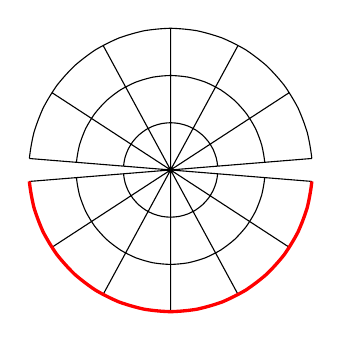
\begin{tikzpicture}
	\pgftransformnonlinear{\circletransformation}
\draw[step=1] (-3,-3) grid (3,3);
\draw[red, very thick] (-3,-3) -- (-3,3);
\end{tikzpicture}
\end{subfigure}
\caption{Transformation $x= r\cos\theta, y= r\sin\theta$}
\end{figure}


\section{Some more geometry}
gravity $\leftrightarrow$ geometry of spacetime

Different (non-Euclidean) geometries possible. Visualization in extra dimension. Also intrinsic definition? 
\begin{itemize}
\item Axiomatic
\item From the distance between nearby points (then larger distances by integration)
\end{itemize}

Any free observer sees the same spacetime, measured with the line element
\[ \diff{s}^2 = \diff{x}^\mu \eta_{\mu\nu}\diff{x}^\nu \]
using the Minkowsky metric. Here we use the mostly plus convention:
\[ \eta = \begin{pmatrix}
-1 & 0 \\
0 & \mathbb{1}_3
\end{pmatrix} \]


\begin{figure}
\centering
\begin{subfigure}{.5\textwidth}
  \centering
    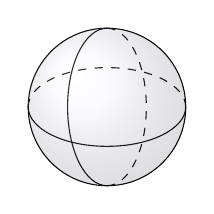
\begin{tikzpicture}
    \draw (-1,0) arc (180:360:1cm and 0.5cm);
    \draw[dashed] (-1,0) arc (180:0:1cm and 0.5cm);
    \draw (0,1) arc (90:270:0.5cm and 1cm);
    \draw[dashed] (0,1) arc (90:-90:0.5cm and 1cm);
    \draw (0,0) circle (1cm);
    \shade[ball color=blue!10!white,opacity=0.20] (0,0) circle (1cm);
\end{tikzpicture}
\end{subfigure}%
\begin{subfigure}{.5\textwidth}
  \centering
    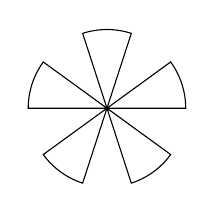
\begin{tikzpicture}
	\foreach \rot in {0,72,...,298} {
\draw[rotate=\rot] (0,0) -- (1cm,0) arc (0:36:1cm) -- (0,0);
}
\end{tikzpicture}
\end{subfigure}
\caption{Positive curvature}
\end{figure}


\begin{figure}
\centering
\begin{subfigure}{.5\textwidth}
  \centering
    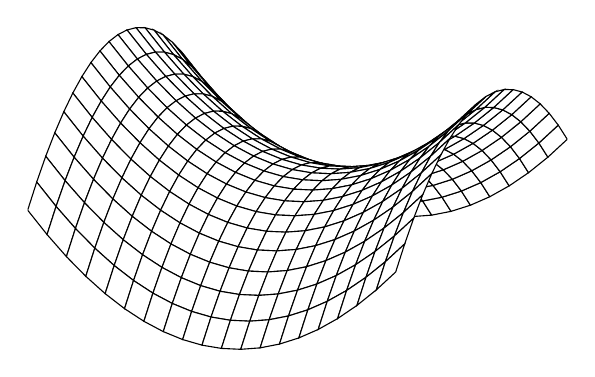
\begin{tikzpicture}
  \begin{axis}[axis lines=none]
    \addplot3[surf, samples=20, color=white, faceted color=black ] {x^2-y^2};
  \end{axis}
\end{tikzpicture}
\end{subfigure}%
\begin{subfigure}{.5\textwidth}
  \centering
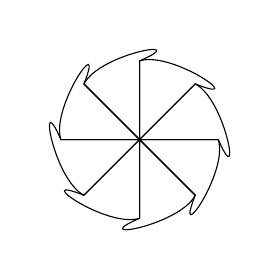
\begin{tikzpicture}
\foreach \rot in {0,45,...,315} {
\draw[rotate=\rot] (0,0) -- (1cm,0) .. controls (1.3cm,-0.7cm) and (1.1cm,.5cm) .. (0.70710678118cm, 0.70710678118cm) -- (0,0);
}
\end{tikzpicture}
\end{subfigure}
\caption{Negative curvature}
\end{figure}

See also intrinsic and extrinsic curvature.
\begin{figure}
\centering
\begin{subfigure}{.5\textwidth}
\caption{Intrinsic curvature}
  \centering
    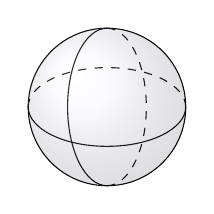
\begin{tikzpicture}
    \draw (-1,0) arc (180:360:1cm and 0.5cm);
    \draw[dashed] (-1,0) arc (180:0:1cm and 0.5cm);
    \draw (0,1) arc (90:270:0.5cm and 1cm);
    \draw[dashed] (0,1) arc (90:-90:0.5cm and 1cm);
    \draw (0,0) circle (1cm);
    \shade[ball color=blue!10!white,opacity=0.20] (0,0) circle (1cm);
\end{tikzpicture}
\end{subfigure}%
\begin{subfigure}{.5\textwidth}
\caption{Extrinsic curvature}
  \centering
    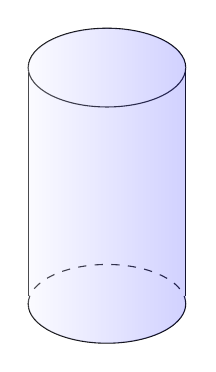
\begin{tikzpicture}
    \draw (-1,0) arc (180:360:1cm and 0.5cm);
    \draw (-1,0) arc (180:0:1cm and 0.5cm);
    \draw (-1,-3) arc (180:370:1cm and 0.5cm);
    \draw[dashed] (-1,-3) arc (180:10:1cm and 0.5cm);
    \draw(-1,-2.9)  -- (-1,0);
    \draw(1,-2.9)   -- (1,0);
    \shade[left color=blue!5!white,right color=blue!60!white,opacity=0.3] (-1,0) arc (180:360:1cm and 0.5cm) -- (1,-3) arc (360:180:1cm and .5cm) -- cycle;
    \shade[left color=blue!5!white,right color=blue!60!white,opacity=0.3] (0,0) circle (1cm and 0.5cm);
\end{tikzpicture}
\end{subfigure}
\caption{Intrinsic and extrinsic curvature}
\end{figure}

\chapter{The equivalence principle}
Given an arbitrary spacetime
\[ \diff{s}^2 = \diff{x}^\mu g_{\mu\nu}(x) \diff{x}^\nu \]
we want the following properties to hold:
\begin{enumerate}
\item Special relativity should be a special case:
\[ g_{\mu\nu}(x) = \eta_{\mu\nu} + \mathcal{O}(x-x_0)^2 \]
\item The same physics should hold for arbitrary transformations
\remark{Coordinates have no meaning}
\item there should be gravity
\end{enumerate}
We have
\[ x^\mu \mapsto x'^\mu = f^\mu(x) \]
with
\[ \diff{x'}^\mu = \Lambda\indices{^\mu_\nu}(x) \diff{x}^\nu \qquad \Lambda \in \GL(1,3) \]
So locally we have a Lorentz group.









\part{Quantum mechanics}
\setcounter{chapter}{0} % Reset chapter counter
\chapter{Measurement theory}

\chapter{Postulates}

\section{States, observables and measurement}
\subsection{States}
\begin{definition}
A \udef{state} on a Hilbert space is a positive trace class operator with trace $1$.
\end{definition}

\begin{proposition}
Let $\rho$ be a state. The following are equivalent:
\begin{enumerate}
\item $\rho$ is extremal;
\item $\rho$ is a projector;
\item $\rho = \rho^2$;
\item $\Tr[\rho^2] = 1$;
\item $\norm{\rho} = 1$;
\item $S(\rho) \defeq -\Tr[\rho\ln\rho] = 0$.
\end{enumerate}
\end{proposition}
The quantity $S(\rho) \defeq -\Tr[\rho\ln\rho]$ is called the \udef{von Neumann entropy}.

\subsection{Effects}
\begin{definition}
An \udef{effect} on a Hilbert space is a bounded operator in $[0,\id]$.
\end{definition}

\chapter{Quantum theory}
\section{Quantum statistics}

\section{Time evolution}
\subsection{The Schrödinger equation}
\[ H = i\hbar\od{}{t} \]

\begin{lemma}
$U = e^{Ht / i\hbar} = e^{-iHt/\hbar}$.
\end{lemma}


\subsection{Schrödinger and Heisenberg pictures}
\begin{lemma}
Let $\mathcal{H}$ be a Hilbert space and $\{e_i\}$ an orthonormal basis. Let $U$ be a unitary operator on $\mathcal{H}$. Then $\{Ue_i\}$ is also an orthonormal basis for $\mathcal{H}$.
\end{lemma}
$\{e_i\}$ gives Schrödinger and $\{Ue_i\}$ gives Heisenberg.



\subsection{Adiabatic theorem}

\begin{theorem}
Let $\mathcal{H}$ be a Hilbert space and consider a path $H: \interval{0,1}\to \SelfAdjoints(\mathcal{H}): s\mapsto H(s)$ of self-adjoint operators on the Hilbert space.

Take $\epsilon >0$. If the Hamiltonian of a system is given by $H(\epsilon t)$ for times $t\in \interval{0,\epsilon^{-1}}$. Then the state $\rho$ of the system satisfies
\[ i\epsilon \od{\rho(s)}{s} = \big[H(s), \rho(s)\big], \]
where $s = \epsilon t \in \interval{0,1}$.

Assume $\lambda(s)\in \spec\big(H(s)\big)$ is an isolated point of the spectrum for all $s\in \interval{0,1}$. It is an eigenvalue and let $P(s)$ be the orthogonal projector onto the eigenspace. Set $\Delta(s) \defeq \inf d\big(\lambda, \spec(H(s))\setminus\{\lambda(s)\}\big)$.

Assume $\rho(0) \leq P(0)$. Consider the fidelity $F(s) \defeq \Tr\big(P(s)\rho(s)\big)$. Then
\[ F(1) \geq 1 - \epsilon O\left(\frac{\norm{H'}^2}{\Delta^3} + \frac{\norm{H^{\prime\prime}}}{\Delta^2}\right). \]
\end{theorem}
\begin{proof}
We first write down a differential equation for the fidelity (where $\prime = \od{}{s}$)
\[ \od{F(s)}{s} = \Tr(P'\rho) + \Tr(P\rho'). \]
The second term is zero because $P$ commutes with $H$:
\begin{align*}
\Tr(P\rho') &= -\epsilon^{-1}i\Tr\Big(P\big[H, \rho\big]\Big) \\
&= -\epsilon^{-1}i\Tr\Big(P(H\rho - \rho H)\Big) \\
&= -\epsilon^{-1}i\Tr\Big(PH\rho\Big) +\epsilon^{-1}i\Tr\Big(\rho HP\Big) \\
&= -\epsilon^{-1}i\Tr\Big(PH\rho\Big) +\epsilon^{-1}i\Tr\Big(\rho PH\Big) \\
&= -\epsilon^{-1}i\Tr\Big(\big[PH, \rho\big]\Big) = 0,
\end{align*}
by \zref{m-traceCommutatorCompactSA}.

Now set $Q(s) = \id - P(s)$ and consider the pseudoinverse $(H-\lambda\id)^+$ (TODO by continuous functional calculus?). Then $(H-\lambda\id)(H-\lambda\id)^+ = Q = (H-\lambda\id)^+(H-\lambda\id)$ by continuous functional calculus (TODO ref). Now we can expand $P' = PP'Q + QP'P$ (by \zref{m-derivativeIdempotentOffDiagonal}), so
\begin{align*}
\od{F(s)}{s} &= \Tr(P'\rho) \\
&= \Tr(PP'Q\rho + QP'P\rho) \\
&= \Tr\Big(PP'(H-\lambda\id)^+(H-\lambda\id)\rho + (H-\lambda\id)(H-\lambda\id)^+P'P\rho\Big) \\
&= \Tr\Big(P'(H-\lambda\id)^+(H-\lambda\id)\rho P + (H-\lambda\id)^+P'P\rho (H-\lambda\id)\Big) \\
&= \Tr\Big(P'(H-\lambda\id)^+\big(H\rho P - \rho \lambda P\big) + (H-\lambda\id)^+P' \big(P\rho H - \lambda P\rho \big)\Big) \\
&= \Tr\Big(P'(H-\lambda\id)^+\big(H\rho - \rho H\big)P + (H-\lambda\id)^+P'P\big(\rho H - H\rho \big)\Big) \\
&= \Tr\Big(P'(H-\lambda\id)^+\big[H,\rho\big]P - (H-\lambda\id)^+P'P\big[H, \rho\big]\Big) \\
&= \Tr\Big(PP'(H-\lambda\id)^+\big[H,\rho\big] - (H-\lambda\id)^+P'P\big[H, \rho\big]\Big) \\
&= \Tr\Big(P'Q(H-\lambda\id)^+\big[H,\rho\big] - (H-\lambda\id)^+QP'\big[H, \rho\big]\Big) \\
&= \Tr\Big(P'(H-\lambda\id)^+\big[H,\rho\big] - (H-\lambda\id)^+P'\big[H, \rho\big]\Big) \\
&= \Tr\Big(\big[P', (H-\lambda\id)^+\big]\cdot\big[H,\rho\big]\Big) \\
&= i\epsilon\Tr\Big(\big[P', (H-\lambda\id)^+\big]\rho'\Big) 
\end{align*}
Integrating this w.r.t. $s$ gives
\[ F(1) - F(0) = i\epsilon\int_0^1 \Tr\Big(\big[P', (H-\lambda\id)^+\big]\rho'\Big)  \diff{s}. \]
We fill in that $F(0) = 1$ and perform integration by parts to obtain
\begin{align*}
F(1) &= 1 + i\epsilon\int_0^1 \Tr\Big(\big[P', (H-\lambda\id)^+\big]\rho'\Big)  \diff{s} \\
&= 1 + i\epsilon\Tr\Big(\big[(H-\lambda\id)^+, P'\big]\rho\Big)_0^1 - i\epsilon\int_0^1 \Tr\Big(\big[(H-\lambda\id)^+, P'\big]'\rho\Big)  \diff{s}
\end{align*}
\end{proof}


\chapter{Approximations}
\section{Approximating eigenvectors}
\subsection{Power series expansion of a non-degenerate level}

\section{Approximating evolutions}

\chapter{Investigations of systems}
\section{Stepped potentials}
(Use density to solve general potentials?)
\section{Coulomb interaction}
\section{Harmonic oscillator}
\chapter{Circuit model}
\section{Qubits}
\begin{definition}
A \udef{qubit} is an element of $\C P^2$.
\end{definition}

\subsection{$\suAlg(2)$ and the Pauli matrices}
The qubit Hamiltonians are elements of $\uAlg(2)$. Getting rid of the arbitrary global phase gives us elements of $\suAlg(2)$.

\begin{lemma} \label{su2Eigenvalues}
For all $\sigma\in \suAlg(2)$, the eigenvalues $\lambda_1, \lambda_2$ are real and $\lambda_1 = -\lambda_2$.
\end{lemma}
\begin{proof}
For all $\sigma\in \suAlg(2)$, $\sigma$ is self-adjoint and $\Tr[\sigma] = \lambda_1 + \lambda_2 = 0$. 
\end{proof}
\begin{corollary}
For all $\sigma\in \suAlg(2)$, we have $\norm{\sigma}_{2} = \sqrt{2}\norm{\sigma}$, where $\norm{\cdot}_2$ is the Hilbert-Schmidt norm.
\end{corollary}
\begin{proof}
We have $\norm{\sigma}_{2} = \sqrt{\lambda_1^2 + \lambda_2^2} = \sqrt{2}|\lambda_1| = \sqrt{2}\norm{\sigma}$.
\end{proof}
\begin{corollary}
The inner product
\[ \inner{\cdot,\cdot}: (\sigma_1,\sigma_2) \mapsto \frac{1}{2}\Tr[\sigma_1\sigma_2] \]
on $\suAlg(2)$ yields the operator norm as the norm associated with this inner product.
\end{corollary}
\begin{corollary} \label{eigenvaluesUnitVectorsu2}
Let $\sigma$ be a unit vector in $\suAlg(2)$. Then $\sigma$ has eigenvalues $\pm 1$. This means $\sigma$ is unitary.
\end{corollary}
\begin{corollary} \label{BlochBijection}
There is a bijection between the unit vectors in $\suAlg(2)$ and the rank-1 projections on $\C^2$ given by $\suAlg(2)/\R \to \sigma\mapsto E^\sigma_{1}$, where $E^\sigma_{1}$ is the eigenspace of $\sigma$ associated with eigenvalue $+1$.
\end{corollary}
\begin{proof}
We construct an inverse of the map. Let $P_1$ be the orthogonal projector on $E^\sigma_{1}$. Then $\sigma = 2P_1 - \id$.
\end{proof}


\begin{proposition}
Let $\sigma\in\suAlg(2)$. Then $\sigma^2 = \norm{\sigma}^2\;\vec{1}$.
\end{proposition}
\begin{proof}
We have 
\[ \sigma^2 = \norm{\sigma}^2 \left(\frac{\sigma}{\norm{\sigma}}\right)^2 = \norm{\sigma}^2 \frac{\sigma}{\norm{\sigma}}\left(\frac{\sigma}{\norm{\sigma}}\right)^* = \norm{\sigma}^2\;\vec{1}, \]
where we have used that $\frac{\sigma}{\norm{\sigma}}$ is unitary by \ref{eigenvaluesUnitVectorsu2}.
\end{proof}
\begin{corollary}
The real algebra generated by $\suAlg(2)$ is the Clifford algebra $\Cl_{3,0}$. The unit pseudoscalar is $i\vec{1}$.
\end{corollary}
Note that $\suAlg(2)$ is a Lie algebra and thus closed under the Lie bracket, but not an algebra under operator composition. Thus the algebra generated by $\suAlg(2)$ is larger than $\suAlg(2)$ (indeed $\sigma^2 = \norm{\sigma}^2\;\vec{1}\notin \suAlg(2)$).

\subsubsection{Pauli matrices}
\begin{proposition}[Pauli matrices]
The Clifford algebra $\suAlg(2)$ has an orthonormal basis
\[ \sigma_x = \begin{pmatrix}
0 & 1 \\ 1 & 0
\end{pmatrix}, \qquad \sigma_y = \begin{pmatrix}
0 & -i \\ i & 0
\end{pmatrix} \qquad \text{and}\qquad \sigma_z = \begin{pmatrix}
1 & 0 \\ 0 & -1
\end{pmatrix}. \]
\end{proposition}

\begin{proposition}
The Pauli matrices obey
\begin{enumerate}
\item $[\sigma_i, \sigma_j] = 2i\leviCivita_{i,j,k}\sigma_k$;
\item $\{\sigma_i, \sigma_j\} = 2\delta_{i,j}\mathbb{1}_2$;
\item $\sigma_i\sigma_j = \delta_{i,j}\mathbb{1}_2 + i\leviCivita_{i,j,k}\sigma_{k}$
\end{enumerate}
\end{proposition}

\begin{corollary}
TODO $\sigma_i\sigma_j\sigma_i = $.
\end{corollary}
eg $\sigma_x\sigma_y\sigma_x = -\sigma_y$.

\subsubsection{Qubit bases}
\begin{definition}
We call
\begin{itemize}
\item the eigenbasis of $\sigma_z$ the \udef{$Z$-basis} or \udef{computational basis} and write the elements
\[ \ket{0} = \begin{pmatrix}
1 \\ 0
\end{pmatrix} \qquad \ket{1} = \begin{pmatrix}
0 \\ 1
\end{pmatrix}; \]
\item the eigenbasis of $\sigma_x$ the \udef{$X$-basis} or \udef{coherence basis} and write the elements
\[ \ket{+} = \frac{1}{\sqrt{2}}\begin{pmatrix}
1 \\ 1
\end{pmatrix} = \frac{\ket{0} + \ket{1}}{\sqrt{2}} \qquad \ket{-} = \frac{1}{\sqrt{2}}\begin{pmatrix}
1 \\ -1
\end{pmatrix} = \frac{\ket{0} - \ket{1}}{\sqrt{2}}. \]
\end{itemize}
\end{definition}

\subsection{The Bloch sphere}
Because $\suAlg(2)$ is the Clifford algebra $\Cl_{3,0}$, we can use the unit sphere in $\R^3$ to represent the unit vectors in $\suAlg(2)$. By \ref{BlochBijection} we can also use it to represent the rank-1 projections on $\C^2$. The unit sphere with as $x,y,z$ axes the Pauli matrices $\sigma_x,\sigma_y, \sigma_z$ is called the \udef{Bloch sphere}.

TODO image of Bloch sphere.

TODO spherical coordinates: $\cos\theta / 2\ket{0} + e^{i\phi}\sin\theta/2 \ket{1}$
\begin{lemma}
\[ e^{\phi/2 i\sigma}e^{\theta/2 i\sigma^\perp}\ket{1} = \cos\theta / 2\ket{0} + e^{i\phi}\sin\theta/2 \ket{1} \]
\end{lemma}

\section{Gates}
\subsection{One-qubit gates}
\subsubsection{Hadamard gate}
\begin{definition}
The \udef{Hadamard gate} or \udef{Walsh-Hadamard gate} $W$ is the linear operation determined by the following matrix:
\[ W = \frac{1}{\sqrt{2}}\begin{pmatrix}
1 & 1 \\ 1 & -1
\end{pmatrix}. \]
\end{definition}
We have the following mappings
\begin{align*}
W\ket{0} &= \ket{+} & W\ket{+} &= \ket{0} \\
W\ket{1} &= \ket{-} & W\ket{-} &= \ket{1}
\end{align*}

\begin{lemma}
The Hadamard gate is its own inverse: $W^2 = \mathbb{1}$.
\end{lemma}

\subsubsection{Pauli gates}
\begin{definition}
Each of the Pauli matrices determines an operation on $\C^2$. In this context we often write $X,Y$ and $Z$ for $\sigma_x, \sigma_y$ and $\sigma_z$.
\end{definition}

\begin{lemma}
The Pauli gates are their own inverses: $X^2 = Y^2 = Z^2 = \mathbb{1}$.
\end{lemma}

\subsection{Controlled gates}
\begin{definition}
Let $H_1, H_2$ be two Hilbert spaces. Let $P$ be a projector on $H_1$ and $L$ an operator on $H_2$. The operation of $L$ \udef{controlled by} $P$ is the operation $P\otimes L + (\id_{H_1} - P)\otimes \id_{H_2}$ in $H_1\otimes H_2 \to H_1\otimes H_2$. 
\end{definition}

\subsection{Two-qubit gates}
\subsubsection{Swap}

\begin{definition}
\[ \begin{quantikz}
&\swap{1}& \\ &\targX{}&
\end{quantikz} \defeq \begin{quantikz}
&\permute{2,1} & \\
& & 
\end{quantikz} \]

$\begin{pmatrix}1&0&0&0\\0&0&1&0\\0&1&0&0\\0&0&0&1\end{pmatrix}$
\end{definition}

\begin{proposition} \label{swapFromCNOT}
\[ \begin{quantikz}
&\swap{1}& \\ &\targX{}&
\end{quantikz} = \begin{quantikz}
&\ctrl{1} & \targ{} & \ctrl{1}& \\
&\targ{} & \ctrl{-1} & \targ{}&
\end{quantikz} \]
\end{proposition}


\chapter{Eigenpath traversal}
\section{Quantum Zeno effect}
\begin{proposition}
Consider a path of states $\ket{\psi(s)}$ where $s\in[0,1]$. Assume that, for fixed $d$ and all $\delta$,
\[ |\braket{\psi(s)}{\psi(s+\delta}|^2 \geq 1-d^2\delta^2. \]
Then 
\end{proposition}

\section{Adiabatic quantum computation}
\section{Evolution through measurement}
\subsection{Phase randomisation}
$\ket{\psi_0} = \ket{E_0(0)} = \sum_i\alpha_i\ket{E_i(s_1)}$
\begin{align*}
\rho(s_1) &= \frac{1}{T}\int_0^T e^{-iH(s_1)t}\ketbra{\psi_0}{\psi_0} e^{iH(s_1)t} \diff{t} \\
&= \sum_{i,j}\alpha_i\alpha_j^* \frac{1}{T}\left(\int_0^T e^{-i(E_i-E_j)t}\diff{t}\right)\ketbra{E_i}{E_j} \\
&= \sum_{i,j}\alpha_i\alpha_j^* \left(\frac{i(e^{-i(E_i-E_j)T}-1)}{T(E_i-E_j)}\right)\ketbra{E_i}{E_j}
\end{align*}

\begin{theorem}[Randomised dephasing]
Let $\ket{\psi(s)}$ be a nondegenerate eigenstate of $H(s)$ and $\{\omega_j\}$ the energy differences to the other eigenstates $\ket{\psi_j(s)}$. Let $T$ be a random variable. Then, for all states $\rho$, we have
\[ \norm{(M_l - e^{-iH(s)T}\rho e^{-iH(s)T}}_\text{tr} \leq \epsilon = \sup_{\omega_j}|\Phi(\omega_j)| \]
\end{theorem}

\chapter{Variational quantum algorithms}

\chapter{Algorithms}
\section{Some building blocks}
\subsection{Preparing states}
\subsubsection{Uniform superposition}
\begin{lemma}
Consider the Hilbert space $\hilbert_{\F_2^k}$. We can generate a uniform superposition of computational basis states by applying a Hadamard gate to each register, initialised to zero:
\[ \frac{1}{2^k}\sum_{b\in \F_2^k}\ket{b} = W^{\otimes k}\ket{0}^{\otimes k}. \]
\end{lemma}

Projection on the $n$-dimensional uniform superposition is given by $\frac{1}{n}\mathbb{J}_{n\times n}$.
\subsection{Quantum Fourier transform}
Set $R_k \defeq \begin{pmatrix}
1 & 0 \\ 0 & e^{2\pi i / 2^k}
\end{pmatrix}$.

TODO: produces swapped result!

Requires $n$ Hadamard gates and $\frac{n(n-1)}{2}$ controlled $R$-gates. At most $n/2$ swaps. Each with three CNOTs (\ref{swapFromCNOT}).

\subsection{Quantum phase estimation}
Needs large number of ancillas.

\begin{proposition}
Let $U$ be a unitary operator and $\ket{\psi}$ an eigenvector of $U$. acting on an $m$-qubit register and . 
\end{proposition}

\subsection{Quantum singular value transformation}

\section{Quantum oracle querying}
\subsection{Oracle set-up}
\begin{definition}
For any finite set $A$, we define a mapping
\[ O: (A\to \F_2) \to \End(\hilbert_{A}\otimes \hilbert_{\F_2}): f\mapsto O_f \]
where
\[ O_f(\ket{k}\otimes \ket{q}) \defeq \ket{k}\otimes \ket{f(k) + q}.  \]
We call $O_f$ the \udef{quantum oracle} of $f$.
\end{definition}

\begin{lemma} \label{phaseUnitaryFromOracle}
We can convert an oracle $O_f$ to a unitary operator $U_f: \hilbert_A\to\hilbert_A: \ket{k}\mapsto (-1)^{f(k)}\ket{k}$ using only a constant number of Hadamard and NOT gates:
\[\begin{quantikz}
\lstick{$\ket{k}$} \qw &  \qw & \qw & \gate[wires=2]{O_f} & \qw & \qw & \qw & \qw \rstick{$U_f \ket{k}$} \\
\lstick{$\ket{0}$} & \gate{X} & \gate{W} & {} & \gate{W} & \gate{X} & \trash{\ket{0}} 
\end{quantikz} \]
If $A$ is finite, then $U_f = \id - 2 \sum_{k\in f^{\preimf}(1)}\ketbra{k}{k}$, which is a Householder matrix.
\end{lemma}
\begin{proof}
We show that the circuit transforms $\ket{k}$ into $(-1)^{f(k)}\ket{k}$.

Given input $\ket{k}$, the oracle acts on $\ket{k}\otimes\ket{-} = \ket{k}\otimes\left(\frac{\ket{0}-\ket{1}}{\sqrt{2}}\right) = \frac{\ket{k}\otimes\ket{0}}{\sqrt{2}} - \frac{\ket{k}\otimes\ket{1}}{\sqrt{2}}$ and produces
\begin{align*}
\frac{\ket{k}\otimes\ket{f(k)}}{\sqrt{2}} - \frac{\ket{k}\otimes\ket{f(k)+1}}{\sqrt{2}} &= \begin{cases}
\ket{k}\otimes\ket{-} & (f(k) = 0) \\
-\ket{k}\otimes\ket{-} & (f(k) = 1) \\
\end{cases} \\
&= (-1)^{f(k)}\ket{k}\otimes\ket{-}.
\end{align*}
Given that $XW$ is the inverse of $WX$, the output $U_f\ket{k}$ is equal to $(-1)^{f(k)}\ket{k}$. The second register is left in the state $\ket{0}$, thus we can either measure of just discard it.

Finally, assume $A$ finite. Then
\begin{align*}
U_f &= U_f\id = U_f\sum_{k\in A}\ketbra{k}{k} = \sum_{k\in f^{\preimf}(0)}U_f\ketbra{k}{k} + \sum_{k\in f^{\preimf}(1)}U_f\ketbra{k}{k} \\
&= \sum_{k\in f^{\preimf}(0)}\ketbra{k}{k} - \sum_{k\in f^{\preimf}(1)}\ketbra{k}{k} \\
&= \sum_{k\in f^{\preimf}(0)}\ketbra{k}{k} - \sum_{k\in f^{\preimf}(1)}\ketbra{k}{k} + \sum_{k\in f^{\preimf}(1)}\ketbra{k}{k} - \sum_{k\in f^{\preimf}(1)}\ketbra{k}{k} \\
&= \left(\sum_{k\in f^{\preimf}(0)}\ketbra{k}{k} + \sum_{k\in f^{\preimf}(1)}\ketbra{k}{k}\right) - 2\sum_{k\in f^{\preimf}(1)}\ketbra{k}{k} \\
&= \id - 2\sum_{k\in f^{\preimf}(1)}\ketbra{k}{k}
\end{align*}
\end{proof}

\subsection{Deutsch's problem}
\begin{problem}
Suppose we have a 1-bit to 1-bit function $f: \{0,1\} \to \{0,1\}: x\mapsto f(x)$.

Determine whether $f$ is
\begin{itemize}
    \item \emph{constant}, i.e.\ $f(0) = f(1)$; or
    \item \emph{balanced}, i.e.\ $f(0) \neq f(1)$.
\end{itemize}
\end{problem}

\begin{proposition}
The classical query complexity of Deutch's problem is 2. The quantum query complexity is 1.
\end{proposition}
\begin{proof}
The classical case is clear.

In the quantum case, we have access to the unitary $U_f: \hilbert_{\F_2}\to \hilbert_{\F_2}$ from \ref{phaseUnitaryFromOracle}. The state $WU_fW\ket{0}$ is as follows:
\begin{align*}
WU_fW\ket{0} &= WU_f\ket{+} = WU_f\left(\frac{\ket{0}+\ket{1}}{\sqrt{2}}\right) \\
&= W\left(\frac{(-1)^{f(0)}\ket{0}+(-1)^{f(1)}\ket{1}}{\sqrt{2}}\right) \\
&= W\begin{cases}
(-1)^{f(0)}\frac{\ket{0} + \ket{1}}{\sqrt{2}} = (-1)^{f(0)}\ket{+} & (f(0) = f(1)) \\
(-1)^{f(0)}\frac{\ket{0} - \ket{1}}{\sqrt{2}} = (-1)^{f(0)}\ket{-} & (f(0) \neq f(1))
\end{cases} \\
&= \begin{cases}
(-1)^{f(0)}\ket{0} & (f(0) = f(1)) \\
(-1)^{f(0)}\ket{1} & (f(0) \neq f(1))
\end{cases}
\end{align*} 
If we measure this state, then we will certainly measure $0$ is $f$ is constant and $1$ if $f$ is balanced.
\end{proof}



\subsection{Grover's search algorithm}
\begin{problem}
Suppose we have a set $\mathcal{N}$ of $N$ items, some of which are marked. WLOG we can take $\mathcal{N}$ to be the set of bit strings of length $\nu$. The marked items form a subset $\mathcal{M}$ of size $M$. Suppose we have an oracle that tells us whether an object is marked or not:
\[ f:\mathcal{N} \to \{0,1\}: x\mapsto \begin{cases}
0 & (x\in \mathcal{M}) \\
1 & (x\notin \mathcal{M})
\end{cases} \]
The problem is to find any marked item.
\end{problem}

Classically we need to check $\Theta(N/M)$ items on average. Grover's algorithm has a query complexity of $O(\sqrt{N/M})$.

\subsubsection{The algorithm}
Define the states
\[ \ket{\mathcal{N}} \defeq \frac{1}{\sqrt{N}}\sum_{n\in\mathcal{N}}\ketbra{n}{n}, \qquad\text{and}\qquad \ket{\mathcal{M}} \defeq \frac{1}{\sqrt{M}}\sum_{m\in\mathcal{M}}\ketbra{m}{m}. \]

Using \ref{phaseUnitaryFromOracle}, construct the unitary $U_f = \id_{\mathcal{H}_N} - 2\sum_{m\in\mathcal{M}}\ketbra{m}{m}$. Also construct the Householder matrix
\[ U = W^{\otimes\nu}(\id - 2\ketbra{0}{0})W^{\otimes\nu} = \id - \mathbb{J}_{2\times 2}^{\otimes\nu} = \id - \mathbb{J}_{2\nu\times 2\nu} = \id - 2\ketbra{\mathcal{N}}{\mathcal{N}}. \]
(TODO Householder circuit).

Now consider the subspace $S \defeq \Span\{\ket{\mathcal{M}}, \ket{\mathcal{N}}\}$. We take an orthonormal basis $\{\ket{\mathcal{M}}, \ket{\mathcal{M}'}\}$ of $S$ where
\[ \ket{\mathcal{M}'} \defeq \sqrt{\frac{N}{N-M}}\ket{\mathcal{N}} - \sqrt{\frac{M}{N-M}}\ket{\mathcal{M}} = \frac{1}{\sqrt{N-M}}\sum_{k\in \mathcal{N}\setminus\mathcal{M}}\ket{k}. \]
Then we can write
\[ \ket{\mathcal{N}} = \sqrt{\frac{N-M}{N}}\ket{\mathcal{M}'}+ \sqrt{\frac{M}{N}}\ket{\mathcal{M}} \]
and (using $\id = \ketbra{\mathcal{M}}{\mathcal{M}} + \ketbra{\mathcal{M}'}{\mathcal{M}'}$)
\begin{align*}
U_f &= \id - 2 \ketbra{\mathcal{M}}{\mathcal{M}} = - \ketbra{\mathcal{M}}{\mathcal{M}} + \ketbra{\mathcal{M}'}{\mathcal{M}'} \\
U &= \id - 2\left(\sqrt{\frac{N-M}{N}}\ket{\mathcal{M}'}+ \sqrt{\frac{M}{N}}\ket{\mathcal{M}}\right)\left(\sqrt{\frac{N-M}{N}}\bra{\mathcal{M}'}+ \sqrt{\frac{M}{N}}\bra{\mathcal{M}}\right) \\
&= \frac{N-2M}{N}\ketbra{\mathcal{M}}{\mathcal{M}} + \frac{2M-N}{N}\ketbra{\mathcal{M}'}{\mathcal{M}'} - 2\left(\frac{\sqrt{M}\sqrt{N-M}}{N}\right)\big(\ketbra{\mathcal{M}}{\mathcal{M}'} +  \ketbra{\mathcal{M}'}{\mathcal{M}}\big)
\end{align*}
So $S$ is invariant under both $U$ and $U_f$ and we can write the matrix $G$ of $-UU_f$ in this basis:
\[ G = \begin{pmatrix}
1 - \frac{2M}{N} & -2 \frac{\sqrt{M}\sqrt{N-M}}{N} \\
2 \frac{\sqrt{M}\sqrt{N-M}}{N} & 1 - \frac{2M}{N}
\end{pmatrix}. \]
We note that $1 - \frac{2M}{N}$ is some number between $-1$ and $1$, so we can write it as $\cos\alpha$. Then
\[ \sin\alpha = \sqrt{1- \cos^2\alpha} = \sqrt{1 - \left(1-2 \frac{M}{N}\right)^2} = \sqrt{4 \frac{M}{N} - 4 \frac{M^2}{N^2}} = 2\sqrt{\frac{M}{N}}\sqrt{1- \frac{M}{N}} = 2 \frac{\sqrt{M}\sqrt{N-M}}{N}. \]
Thus
\[ G = \begin{pmatrix}
\cos\alpha & -\sin\alpha \\
\sin\alpha & \cos\alpha
\end{pmatrix} = R_\alpha. \]
We now want to apply $G$ a certain number of times, say $k$, such that
\[ G^k\ket{\mathcal{N}} = G^k \begin{pmatrix}
\sqrt{M/N} \\ \sqrt{1 - M/N}
\end{pmatrix} = R_{k\alpha}R_{\tan^{-1}(\sqrt{N/M - 1})} \begin{pmatrix}
1 \\ 0
\end{pmatrix} \approx \begin{pmatrix}
1 \\ 0
\end{pmatrix} = \ket{\mathcal{M}}. \]

TODO:
\[ \sqrt{\frac{N}{M}} \approx T_k(\cos\alpha) - \sqrt{\frac{N}{M} - 1}U_{k-1}(\cos\alpha) \]
or
\[ 0 \approx \sqrt{\frac{N}{M}-1}T_k(\cos\alpha) + U_{k-1}(\cos\alpha)\sin\alpha \]
and
\[ (\cos\alpha + \sin\alpha)^k = T_k(\cos\alpha) + \sin\alpha U_{k-1}(\cos\alpha). \]

We also have $\cos\alpha + \sin\alpha = \frac{(\sqrt{N-M}-\sqrt{M})^2+2M}{N}$.

\subsubsection{Analogue Grover}
Consider the Hamiltonian $H = \ketbra{\mathcal{M}}{\mathcal{M}} + \ketbra{\mathcal{N}}{\mathcal{N}}$, which we can rewrite in terms of $\ket{\mathcal{M}}$ and $\ket{\mathcal{M}'}$:
\[ H = \left(1 + \frac{M}{N}\right)\ketbra{\mathcal{M}}{\mathcal{M}} + \left(1 - \frac{M}{N}\right)\ketbra{\mathcal{M}'}{\mathcal{M}'} + \frac{\sqrt{M}\sqrt{N-M}}{M}\Big(\ketbra{\mathcal{M}}{\mathcal{M}'}+\ketbra{\mathcal{M}'}{\mathcal{M}}\Big), \]
This operator is self-adjoint and leaves the subspace $S$ invariant, so $S$ has a basis of eigenvectors for it.

By \zref{m-eigenvectorsGenerator}, all elements of $e^{-iHt}\ket{\mathcal{N}}$ lie in $S$. W.r.t.\ the basis $\{\ket{\mathcal{M}}, \ket{\mathcal{M}'}\}$, we have
\[ e^{-iHt}\ket{\mathcal{N}} = \begin{pmatrix}
\sqrt{M/N}\cos(\sqrt{M/N}t) - i\sin(\sqrt{M/N}t) \\ \sqrt{1- M/N}\cos(\sqrt{M/N}t)
\end{pmatrix}. \]
Thus $\braket[e^{-iHt}]{\mathcal{M}}{\mathcal{N}} = \frac{M}{N}\cos^2(\sqrt{M/N}t) + \sin^2(\sqrt{M/N}t)$. This is equal to 1 when $t = \frac{\pi}{2}\sqrt{\frac{N}{M}}$.

Thus we can produce $\ket{\mathcal{M}}$ in $O(\sqrt{N/M})$ time.

TODO: optimality.

\subsubsection{Adiabatic Grover}
\[ H_0 = \vec{1} - \ketbra{\mathcal{N}}{\mathcal{N}} = \mathbb{1}-\mathbb{J}/N \]
\[ H_f = \vec{1} - \sum_{m\in\mathcal{M}}\ketbra{m}{m} = \begin{pmatrix}
0 & 0 \\ 0 & \mathbb{1}_{N-M}
\end{pmatrix}.\]

Then
\[ H(s) = (1-s)H_0 + sH_f = \begin{pmatrix}
(1-s)\mathbb{1} +\frac{s-1}{N}\mathbb{J} & \frac{s-1}{N}\mathbb{J} \\
\frac{s-1}{N}\mathbb{J} & \mathbb{1} + \frac{s-1}{N}\mathbb{J}
\end{pmatrix} = \begin{pmatrix}
(1-s)\mathbb{1}_M & 0 \\ 0 & \mathbb{1}_{N-M}
\end{pmatrix} + \frac{s-1}{N}\mathbb{J}. \]
Then, setting $A = \begin{pmatrix}
(1-s-\lambda)\mathbb{1}_M & 0 \\ 0 & (1-\lambda)\mathbb{1}_{N-M}
\end{pmatrix}$
\begin{align*}
\det(H(s)-\lambda) &= \det \left(A + \frac{s-1}{N}\mathbb{J}^{n\times 1}\mathbb{J}^{1\times n}\right) \\
&= \det(A)\det \left(\mathbb{1}_N + \frac{s-1}{N}A^{-1}\mathbb{J}^{n\times 1}\mathbb{J}^{1\times n}\right) \\
&= \det(A)\det \left(1 + \frac{s-1}{N}\mathbb{J}^{1\times n}A^{-1}\mathbb{J}^{n\times 1}\right) \\
&= (1-s-\lambda)^{M}(1-\lambda)^{N-M}\left(1 + \frac{M(s-1)}{(1-s-\lambda)N} + \frac{(N-M)(s-1)}{(1-\lambda)N}\right) \\
&= (1-s-\lambda)^{M-1}(1-\lambda)^{N-M-1}\left(\lambda^2 - \lambda + s(1-s)\frac{N-M}{N}\right),
\end{align*}
where we have used the matrix determinant lemma to simplify the calculation.

We see that there are four distinct eigenvalues:
\begin{align*}
\lambda_{0,1} &= \frac{1}{2}\left(1\pm \sqrt{1-4(1- \frac{M}{N})s(1-s)}\right) &\text{with multiplicity $1$} \\
&= \frac{1}{2}\left(1\pm \sqrt{\frac{M}{N}+4(1- \frac{M}{N})(s-\frac{1}{2})^2}\right) \\
\lambda_{2} &= 1-s &\text{with multiplicity $M-1$}\\
\lambda_{3} &= 1 &\text{with multiplicity $N-M-1$.}
\end{align*}

Define $\Delta \defeq \lambda_1-\lambda_0 = \sqrt{1-4(1- \frac{M}{N})s(1-s)}$.
TODO: we can ignore $\lambda_{2,3}$! (Why?)

\begin{lemma}
\[ \int_0^1 \frac{1}{\Delta}\diff{s} = \sqrt{\frac{\frac{N}{M}}{4\big(\frac{N}{M}-4\big)}}\log\Bigg(\frac{\sqrt{\frac{N}{M}\big(\frac{N}{M}-1\big)}+ \big(\frac{N}{M}-1\big)}{\sqrt{\frac{N}{M}\big(\frac{N}{M}-1\big)}- \big(\frac{N}{M}-1\big)}\Bigg) \sim \log\Big(\frac{N}{M}\Big). \]
\end{lemma}

Next we are interested in the eigen vectors associated to $\lambda_{0,1}$. Let $Q_1$ be a unitary transformation that maps $\mathbb{J}^{M\times 1}$ to $\begin{pmatrix}
\sqrt{M} \\ 0 \\ 0 \\ \vdots
\end{pmatrix} \in \C^M$. Similarly let $Q_2$ be a unitary transformation that maps $\mathbb{J}^{(N-M)\times 1}$ to $\begin{pmatrix}
\sqrt{N-M} \\ 0 \\ 0 \\ \vdots
\end{pmatrix} \in \C^{(N-M)}$ and define $Q = \begin{pmatrix}
Q_1 & 0 \\ 0 & Q_2
\end{pmatrix}$, which is also unitary. Then we have
\begin{align*}
    QH(s)Q^{-1} &= \begin{pmatrix}
        (1-s)\mathbb{1}_M & 0 \\ 0 & \mathbb{1}_{N-M}
        \end{pmatrix} + \frac{s-1}{N}Q\mathbb{J}^{N\times 1}(\mathbb{J}^{N\times 1})^*Q^* \\
    &= \begin{pmatrix}
        (1-s)\mathbb{1}_M & 0 \\ 0 & \mathbb{1}_{N-M}
        \end{pmatrix} + \frac{s-1}{N} \begin{pmatrix}\sqrt{M} \\ 0 \\ \vdots \\ 0 \\ \sqrt{N-M} \\ 0 \\ \vdots \end{pmatrix}\begin{pmatrix}\sqrt{M} \\ 0 \\ \vdots \\ 0 \\ \sqrt{N-M} \\ 0 \\ \vdots \end{pmatrix}^*.
\end{align*}

All but two of the eigenvectors are just elements of $\mathcal{N}$. To study the other two we can simplify by ``removing the zeros''. Now the eigenvalue problem becomes
\[ \left(\begin{pmatrix}
1-s-\lambda_{0,1} & 0 \\ 0 & 1 -\lambda_{0,1}
\end{pmatrix} + \frac{s-1}{N}\begin{pmatrix}
\sqrt{M} \\ \sqrt{N-M}
\end{pmatrix}\begin{pmatrix}
\sqrt{M} \\ \sqrt{N-M}
\end{pmatrix}^*\right)\vec{v} = 0. \]
Setting $\vec{v} = \begin{pmatrix}
x_1 \\ x_2
\end{pmatrix}$ gives us the equations
\begin{align*}
0 &= (1-s-\lambda_{0,1})x_1 + \frac{s-1}{N}(Mx_1 + \sqrt{M}\sqrt{N-M}x_2) \\
0 &= (1-\lambda_{0,1})x_2 + \frac{s-1}{N}(\sqrt{M}\sqrt{N-M}x_1 + (N-M)x_2)
\end{align*}
reshuffling and dividing these equations gives
\[ \frac{(1-s-\lambda_{0,1})x_1}{(1-s-\lambda_{0,1})x_2} = \frac{-\frac{s-1}{N}(Mx_1 + \sqrt{M}\sqrt{N-M}x_2)}{-\frac{s-1}{N}(\sqrt{M}\sqrt{N-M}x_1 + (N-M)x_2)} = \frac{\sqrt{M}(\sqrt{M}x_1 + \sqrt{N-M}x_2)}{\sqrt{N-M}(\sqrt{M}x_1 + \sqrt{N-M}x_2)} = \frac{\sqrt{M}}{\sqrt{N-M}}. \]
So we have eigenvectors $\vec{v}_{0,1} = (\sqrt{M}(1-\lambda_{0,1}), \sqrt{N-M}(1-s-\lambda_{0,1}))^\transp$ of $QH(s)Q^{-1}$. The corresponding eigenvectors of $H(s)$ are then given by
\[ Q^*\vec{v}_{0,1} = \begin{pmatrix}
(1-\lambda_{0,1})\mathbb{J}^{M\times 1} \\ (1-s-\lambda_{0,1})\mathbb{J}^{(N-M)\times 1}
\end{pmatrix}. \]

For computational ease we will keep on working with the eigenvectors $\vec{v}_{0,1}$ of $QH(s)Q^{-1}$. We denote by $\ket{0}$ and $\ket{1}$ the normalisation of $\vec{v}_{0,1}$.


\subsubsection{Poisson projective measurement}
The dynamics of the system is governed by the differential equation
\[ \od{\rho}{s} = \Lambda(\ketbra{0}{0}\rho \ketbra{0}{0} + \ketbra{1}{1} \rho \ketbra{1}{1} - \rho). \]
Now we can rewrite $\od{\rho}{t}$ in the basis $ \ket{0}, \ket{1}$: let $i,j,k,l=0,1 \mod 2$ with implicit summation
\begin{align*}
\od{\rho}{s} &= \od{}{s}\left(\ketbra{i}{i}\rho\ketbra{j}{j}\right) \\
&= \od{}{s}(\braket[\rho]{i}{j})\ketbra{i}{j} + \braket[\rho]{i}{j}\od{}{s}(\ketbra{i}{j}) \\
&= \od{}{s}(\braket[\rho]{i}{j})\ketbra{i}{j} + \braket[\rho]{i}{j}\ketbra{k}{k}\od{}{s}\ketbra{i}{j} - \braket[\rho]{i}{j}\ketbra{i}{j}\od{}{s}\ketbra{l}{l} \\
&= \od{}{s}(\braket[\rho]{i}{j})\ketbra{i}{j} + \braket[\rho]{i}{j}\ketbra{i+1}{i+1}\od{}{s}\ketbra{i}{j} - \braket[\rho]{i}{j}\ketbra{i}{j}\od{}{s}\ketbra{j+1}{j+1} \\
&= \left(\od{}{s}(\braket[\rho]{i}{j}) + \braket[\rho]{i+1}{j}\braket[\od{}{s}]{i}{i+1}  - \braket[\rho]{i}{j+1}\braket[\od{}{s}]{j+1}{j}\right)\ketbra{i}{j}. \\
\end{align*}
For each $\ketbra{i}{j}$ we get an equation, four in total. One of these is redundant by the zero trace requirement. Writing $y_{i,j}\defeq \braket[\rho]{i}{j})$ and $\omega_{ij} \defeq \braket[\od{}{s}]{i}{j}$ the three remaining equations are
\begin{align*}
\od{\rho_{00}}{s} &= -\rho_{10}\omega_{01} + \rho_{01}\omega_{10} \\
\od{\rho_{01}}{s} &= -\Lambda \rho_{01} - (1-\rho_{00})\omega_{01} + \rho_{00}\omega_{01} \\
\od{\rho_{10}}{s} &= -\Lambda \rho_{10} - \rho_{00}\omega_{10} + (1-\rho_{00})\omega_{10}
\end{align*}
Setting $\omega = \omega_{10} = - \omega_{01}$ and $y = \rho_{00} - 1/2$we obtain the equation
\[ \od[2]{y}{s} = \left(\frac{\od{\omega}{s}}{\omega}-\Lambda\right)\od{y}{s} - 4\omega^2y. \]


Setting $\vec{y} = \begin{pmatrix}
y \\ y'
\end{pmatrix}$ this second order differential equation is equivalent to the first order system
\[ \begin{pmatrix}
y \\ y'
\end{pmatrix}' = \begin{pmatrix}
0 & 1 \\ -4 & -\Lambda/\omega
\end{pmatrix}, \]
which is in the form $\vec{y}' = A \vec{y}$. Now $A$ is similar to $\begin{pmatrix}
    \omega/\Lambda & 0 \\ -4 & -\Lambda/\omega
\end{pmatrix}$, so it is bounded if both $\Lambda$ and $\Lambda^{-1}$ are bounded functions.

Then by the Picard-Lindelöf theorem the initial value problem has a unique solution on $[0,1]$. In addition let $y_1$ be the solution obtained using $\Lambda_1$ and $y_2$ using $\Lambda_2$. Then
\[ \Lambda_1 \leq \Lambda_2 \implies y_1 \leq y_2. \]
To see this, we may first remark that
\[ \setbuilder{t\in[0,1]}{y_1(t)\leq y_2(t) \land y'_1(t)\leq y'_2(t)} = (y_2-y_1)^{-1}[\;[0,+\infty[\;] \cap (y'_2-y'_1)^{-1}[\;[0,+\infty[\;] \]
is a closed and bounded set that contains $0$. Let $t_1$ be its supremum. This means that $y_1(t_1)\leq y_2(t_1)$ and $y'_1(t_1)\leq y'_2(t_1)$, but $y_1(t) > y_2(t)$ or $y'_1(t) > y'_2(t)$ on some open set $]t_1, t_1+\delta [$.








Now we move onto the second of Lord Kelvin's clouds, which has to do with the equipartition theorem of classical statistical mechanics. One obvious way in which the classical theory fails is when we look at thermal radiation. Object at any temperature emit electromagnetic radiation. The hotter the object, the more it emits (it becomes ``glowing hot''). Unfortunately classical theory predicts that all objects emit an infinite amount of radiation of very short wavelength (i.e. ultraviolet radiation). This is clearly not true and is known as the ultraviolet catastrophe.

It was this problem that Planck solved in December of 1900. The way he solved it and the assumptions he made in order to solve it had profound implications and let to the development of quantum mechanics.

As with relativity we will first go through some of the seminal experiments for quantum mechanics in order to gain a sense of the phenomenology, then based on the phenomena we will have discussed, we will develop the theory of quantum mechanics.

Quantum mechanics is quite a bewildering field that makes very little intuitive sense. The \textit{mathematics} of quantum mechanics is well understood and has yielded many thoroughly tested predictions. At this point it is a mature theory, so it's quite surprising we still have not quite figured out what exactly it \textit{means}. There are several competing interpretations of quantum mechanics, which we shall very briefly mention below. These interpretations do not disagree on what they predict we observe, only on what is actually happening. Thus one may surmise that they are more philosophical in nature and not necessarily relevant to the student of physics. This instrumentalist view is prevalent in many quantum mechanics courses where it is much easier, rather than wade into the murky philosophical depths of our lack of understanding, to just quote David Mermin: "Shut up and calculate".

Unfortunately for us, this multitude of post hoc interpretations poses a serious problem for our project of Carnappian rational reconstruction: which conception of reality do we base our reconstruction on and why? Recently a possible answer to this quandary has started to emerge: quantum informational axiomatisations have emerged that do not rely on our accepting any one interpretation of quantum mechanics. This is a rather new field of research and not all problems have been ironed out yet, nevertheless it is an interesting if somewhat unsatisfactory avenue and we have a quick glance down it.

Bearing this in mind, this part on quantum mechanics is structured as follows: first we have a look at some of the strange phenomena that could not be explained classically and motivated the development of quantum mechanics; at the same time we will briefly mention some of the early ad hoc theories to explain these phenomena. These theories are now sometimes referred to as the old quantum theories and still find use as semi-classical approximations. We will then have a look at the two theories that were invented in order to explain these phenomena: matrix mechanics and wave mechanics, with an emphasis on wave mechanics because it is conceptually simpler. The introduction of these theories is still somewhat ad hoc, but they do manage to explain all of the quantum phenomena. The next step is a generalization to the elegant modern formulation of quantum mechanics using separable Hilbert spaces and a statement of the Dirac-von Neumann axioms (or postulates as they are often called). We will do our best to justify why these axioms are natural but, for the reasons mentioned above, the results of this effort will remain somewhat unsatisfactory. At this point some of the interpretations of this theory we have just constructed will be mentioned.

\chapter{Origins and justification}
\section{Wave-particle duality}
\subsection{A history of particle and wave theories of light}
The nature of light has long been the subject of debate, going all the way back to the ancient Greeks. In the $11^\text{th}$ century the Arabic scientist Ibn al-Haytham (also known as Alhazen) wrote the comprehensive Book of Optics describing such phenomena as reflection and diffraction. He asserted that light rays are composed of particles of light.

In 1630 championed the wave theory of light. All other known waves had to propagate through a medium, so he posited the existence of a universal medium, the luminiferous aether.

In Opticks, published in 1704, Isaac Newton defended his corpuscular (i.e. particle) theory. He argued that only particles could move in the perfectly straight lines of light rays.

Around the same time others (including Robert Hooke, Christiaan Huygens and Augustin-Jean Fresnel) were refining the wave viewpoint.

In 1801 Thomas Young proposed his infamous double-slit experiment demonstrating wave interference of light. This, in conjunction with the inability of the particle theory to explain polerisation, began to convince the scientific community and by the middle of the $19^\text{th}$ century the wave theory was generally accepted.

In the second half of the $19^\text{th}$ century James Clerk Maxwell discovered that his equations could be applied to describe self-propagating waves of the electric and magnetic fields. It quickly became apparent that visible light, ultraviolet light and infrared light were all just electromagnetic waves of different frequencies.

\subsection{The particle nature of photons}
\subsubsection{Black body radiation}
In the section on optics (TODO) we have seen the form the spectral distribution of black body radiation takes (figure TODO). We have also already given some results based on general thermodynamic results. In order to derive an actual expression for the spectral distribution function $\rho(\lambda, T)$ we need a more detailed model.

TODO

$h$ gives quantum of action
seen as a mathematical trick by Planck trick

Wall of cavity never in equilibrium with radiation: finite degrees of freedom v infinite degrees of freedom.

\subsubsection{The photoelectric effect}
While Heinrich Hertz was performing his celebrated experiments in 1887 producing and detecting electromagnetic waves, experimentally verifying Maxwell's theory, he discovered a peculiar phenomenon: ultraviolet light falling on electrodes facilitates the passage of a spark. It was shown that this was due to electrons being ejected from the metallic surfaces when irradiated by high-frequency electromagnetic waves. This effect is called the \udef{photoelectric effect}.

Clearly the incident electromagnetic radiation is exciting the electrons in the metal enough to break free of their bonds. The photoelectric effect has a number of features that are impossible to explain with the classical theory of electromagnetic waves. Remember that in classical theory the energy of electromagnetic radiation depends on the intensity of the beam, but is independent of the frequency. (TODO:?)
\begin{enumerate}
\item There is a cutoff frequency below which no emission of electrons takes place, no matter the intensity of the beam.
\item The maximum kinetic energy of the emitted electrons depends linearly on frequency and is independent of the intensity.
\item Emission takes place immediately when light shines on the surface, there is no detectable time delay between exposure to light and emission of electrons. Based on classical theory we would expect to have a delay when using low intensity beams because it would take time to pump enough energy into a region of space of atomic proportions.
\end{enumerate}
A very the solution to these problems was proposed in 1905 by Einstein. It was for this paper that he got the Nobel prize. Einstein proposed that we take the quantization that Max Planck had introduced seriously, and not just view it as a mathematical trick. His assertion was that light consists of quanta, now called \udef{photons}, each with an energy
\[ E = h\nu = hc / \lambda. \]
The strange phenomena described above can then be explained as follows:
\begin{enumerate}
\item A single photon needs to carry enough energy to eject an electron from the surface. (The energy required to do that is called the \udef{work function} $W$ and depends on the metal being irradiated). Thus if the frequency is too low, no electrons are emitted, no matter how many photons are pumped into the system (i.e. how high the intensity is).
\item When a photon collides with an electron, it is absorbed and passes (almost) all of its energy on to the electron, thus the maximum kinetic energy of emitted electrons is the energy of the photons ($h\nu$) minus the work function.
\item If energy is not constantly being pumped into an electron, it quickly loses the energy it gained (I assume?? TODO). Thus, because the electrons receive energy from photons in small - quantized - bursts, there is no mechanism by which energy can accumulate to a point where the electron is able to break free from the bulk metal. This means emission is either instantaneous, or does not happen.
\end{enumerate}
So in conclusion, the photoelectric effect provides compelling evidence for the corpuscular nature of light. Unfortunately there is also a large amount of evidence confirming that light travels in waves. Quantum mechanics gives us a model for photons that exhibits both wave-like and particle-like behaviour. This is know as ``wave-particle duality''.


\subsubsection{The Compton effect}
Another phenomenon that helps confirm the particular nature of light is the Compton effect, named after Arthur Holly Compton. This effect occurs when irradiating matter (Compton used graphite) with X-rays. Some of the X-rays are scattered omni-directionally with no change in wavelength. This is known as \udef{Thomson scattering} and can be explained classically. Sometimes the X-rays are also scattered such that the scattered wave has a different wavelength, especially if the incident X-rays have a short wavelength. Even more strangely the wavelength of the scattered wave depends on the angle at which it is scattered. This is known as \udef{Compton scattering}. The difference between the wavelength of the incident wave and the scattered wave is called the \udef{Compton shift}.

Thomson scattering can be explained (classically) as follows: The incident oscillating electric field causes the atomic electrons to oscillate at the same frequency. These electron then radiate electromagnetic radiation in all directions at the same frequency.

Compton scattering can be explained if we assume the incident X-rays are made up of corpuscular X-rays that scatter the atomic electrons like particles. The process is very similar to the photoelectric effect, but Compton did not build on Einstein's work. The difference is that energy of the incident photon is higher and thus the photon is not absorbed, but merely relinquishes some of its energy to the electron during the scattering process and can be detected when it comes out of the sample of matter being irradiated. In fact the Compton and photoelectric effects are two of the three competing effects when photons interact with matter; the third is pair production and is dominant at even higher energies. (These effects will be discussed in more detail later).

Because scattered can only be detected if their energy is significantly higher than the binding energy of the electrons with the atoms, we can simplify our calculations by assuming the electrons are \textit{free}, i.e. not bound to any atoms. This explains why the expression for the Compton shift is independent of the nature of the material used for the target. The scattering probability does of course depend on the target and is in particular directly proportional to the density of electrons.

Assuming the incident photon is a particle (TODO image), we can use conservation of relativistic energy and momentum to derive the following equation:
\[ \lambda_s - \lambda_0 = \Delta \lambda = \frac{2h}{m_e c}\sin^2(\theta/2) \]
where $\lambda_0$ and $\lambda_s$ are the wavelength of the incident and scattered X-rays respectively; $m_e$ is the mass of an electron.

Thomson scattering (i.e. scattering with $\lambda_s = \lambda_0$) can be explained in this model by assuming it results from scattering by electrons bound so tightly that the whole atom recoils. In this case we should use the mass $M$ of the whole atom and the Compton shift $\Delta \lambda$ becomes negligible.

\subsection{The wave nature of matter: the de Broglie hypothesis}
In 1923 it was generally accepted that electromagnetic radiation can exhibit both wave-like and particle-like behaviour. In 1923 / 1924 Louis de Broglie proposed that matter may also have this dual nature. He postulated that the Planck-Einstein formula for the energy of a photon
\[ E  = h\nu \]
is not a peculiar feature of photons but holds for all particles. This means there must be some way to associate a wavelength to a particle. This wavelength is called the \udef{de Broglie wavelength} in his honor and is given by
\[ \lambda = \frac{h}{p}. \]
What is unique to photons is the relation $\lambda\nu = c$ making this second relation redundant and setting $p = E / c$ for photons.

\subsubsection{Electron diffraction}
If we compare with the results of classical optics, we realise that we will only be able to verify de Broglie's hypothesis by observing interference and diffraction effects if the length of some relevant part of the measurement setup is comparable to the wavelength. So in order to hope to measure electron diffraction, it is useful to have an idea of the de Broglie wavelength of an electron.

Let us assume we are producing a beam of electrons by accelerating them across a potential difference $V_0$, so that the kinetic energy is $mv^2/2 = eV_0$. In the non-relativistic limit, the momentum is given by $p=mv$ and thus the de Broglie wave length is given by
\[ \lambda = \frac{h}{mv} = \frac{h}{\sqrt{2meV_0}} \approx \frac{12.3}{\sqrt{V_0[\text{Volts}]}}\si{\angstrom} \]

This is much smaller than any length we would usually come across, which is why we had not realised matter had a wave-like nature, but is comparable to the spacing between atoms in a crystal. Using the theory developed by Bragg, Laue and others for the diffraction of X-rays by crystals (which will be developed later in the section on solid state physics), George Paget Thomson (son of J.J. Thomson, who gave his name to Thomson scattering among many other things), and Clinton Davidson and Lester Germer independently gave experimental evidence that electrons do indeed exhibit a wave-like nature.

Subsequent experiments have shown that other particle - protons, neutrons and even molecules - can exhibit wave-like behaviour.

\subsection{Wave-packets}
\subsubsection{Form of the wave}
So we seem to be able to associate something that behaves like a wave to matter.

Meaning? Spread out in space.

TODO after fluid dynamics. Decomposition into packets.
\subsubsection{Correspondence principle}
TODO image of broad wave to Dirac delta.

For almost all macroscopic physics, classical physics is obviously still a very good approximation.

Classically not spread out in space, but localised.  thus with vanishing wavelength. Here we may draw the parallel with geometrical optics which is the short-wavelength limit of wave optics. 
\subsubsection{The Heisenberg uncertainty principle}
De Broglie's original paper.

\subsection{Double-slit experiments}
Thomas Young's double-slit experiment can neatly be summed up by figure TODO (include labels of light source and screen). The image on the screen is then something like figure TODO(b). TODO: move to optics??

Similar experiments can be used to show the wave nature of electrons and other particles. In these cases it is much easier to record individual particles, and we get an image on the screen resembling figure TODO.

With light the interference pattern can be explained by the fact that
\begin{enumerate}
\item The amplitudes of the light-waves can be added linearly;
\item The intensity is given by the square of the amplitude.
\end{enumerate}

In the classical view, the interpretation of these statements is relatively clear: the amplitudes of the light-waves are the amplitudes of the oscillations of the electric and magnetic fields. The intensity is the power per unit area and can be measured by our eyes (TODO: see optics!!).

If we try applying this to matter that is classically thought of as consisting of particles, we run into some problems: How come we can (only) measure single electrons? Electrons invariably show up as blips on our detectors, we seem not to be able to detect the waves directly.

In light of this we may think that electrons are in essence particles and the wave-like features we measure are simply the result of interactions between electrons we do not understand yet. This turns out not to be the case. Experiments have been performed with very weak sources over the course of weeks such that there is only ever at most one electron traveling through the double-slit apparatus. These experiments yield exactly the same interference patterns.

So it seems very likely that the two aspects of classical theory that allow these interference patterns to occur have quantum analogues. 

\subsubsection{Statistical interpretation}
Max Born hypothesised an interpretation 

\subsubsection{Superposition principle}


\section{Quantised quantities}
TODO: Planck postulated quantisation of energy. There are several other phenomena and experiments that can be explained much more easily if we assume certain quantities to be quantised.
\subsection{Atomic spectra}
\subsubsection{Bohr model of the hydrogen atom}
Quantised energy and angular momentum

\subsection{Franck and Hertz experiment}
Quantisation of energy.

\subsection{Stern-Gerlach experiment}
Angular momentum and spin

\section{A history of quantum theories}


In 1925 / 1926 two different (but ultimately equivalent) theories were put forward to describe the properties of quantum mechanical objects, \textit{matrix mechanics} developed by Werner Heisenberg, Max Born and Pascual Jordan, and \textit{wave mechanics} developed by Erwin Sch\"odinger. Both are particular forms of a more general formulation of quantum mechanics developed by Paul Adrian Maurice Dirac in 1930.


\section{Wave mechanics}
\subsection{Schr\"odinger equation}
\[ E= \frac{\vec{p}^2}{2m}+V(\vec{x}) \]
Make the following substitutions:
\[ E \to i \pd{}{t}, \qquad \vec{p} \to -i \vec{\nabla}, \qquad \vec{x} \to \vec{x} \]
And we get Schrödinger's equation
\[ \boxed{i \pd{\psi}{t} = \left(- \frac{\nabla^2}{2m}+V(x)\right)\psi} \equiv H\psi \]
We are going to study conservative systems, so $H$ does not depend on time.
\subsection{Bohr condition}
\[\rho(\bar{x},t) = \left|\psi(x)\right|^2 \geq 0 \]
\[ P(t) = \int_{\R^3} \diff{^3x}\rho(x,t) = \int \diff{^3x}\left|\psi(\bar{x},t)\right|^2 = 1 \]
So $\psi \in \mathcal{C}_2$
\subsection{Is the probability constant in time?}
\begin{align*}
\od{P}{t} &= \int_{\R^3}\diff{^3x}\pd{}{t}\left|\psi(x,t)\right|^2 = \int_{\R^3}\diff{^3x}\left(\pd{\psi^*}{t}\psi + \psi^*\pd{\psi}{t}\right) \\
&= \frac{i}{2M}\int_{\R^3} \diff{^3x}\left(\psi^*\left(\bar{\nabla}^2\psi\right)- \cancel{V\psi^*\psi\cdot2M} - \left(\bar{\nabla}^2\psi^*\right)\psi + \cancel{V\psi^*\psi\cdot2M}\right) \\
&= \frac{i}{2M}\int_{\R^3}\diff{^3x}\bar{\nabla}\cdot \left(\psi^*\left(\bar{\nabla}\psi\right)- \left(\bar{\nabla}\psi^*\right)\psi\right) \\
\vec{j}(\bar{x},t) &\equiv \frac{-i}{2M}\left(\psi^*\left(\bar{\nabla}\psi\right)- \left(\bar{\nabla}\psi^*\right)\psi\right)
\end{align*}
So we get
\[ \od{P}{t} = -\int_{\R^3}\vec{\nabla}\cdot \vec{j}\diff{^3x} = -\oint_{\partial \R^3} \vec{j}\cdot \vec{u}_j \diff{^2\sigma} = 0 \]
Where
\[ \begin{cases}
\vec{j}(\bar{\infty},t) = 0\\
\psi(\bar{\infty},t) = 0 \qquad \text{because} \quad \psi \in \mathcal{C}_2
\end{cases} \]
(Assumption of conservative system important!)
\subsection{Continuity equation}
\[ \pd{}{t}\left|\psi(\bar{x},t)\right|^2 + \vec{\nabla}\cdot\vec{j} = 0 \]
Conservation of probability = continuity equation

\subsection{One-dimensional examples}
\subsubsection{The linear quantum harmonic oscillator.}
We have a potential of the form
\[ V(x) = \frac{1}{2}kx^2 \]
so the Schrödinger equation becomes
\[ - \frac{\hbar^2}{2m}\od[2]{\psi(x)}{x} + \frac{1}{2}kx^2\psi(x) = E\psi(x) \]
We can immediately see that all eigenfunctions correspond to bound states of positive energy.
\subsection{Three-dimensional examples}



\subsection{General solution of the free Schrödinger equation}
\[ \boxed{i \pd{}{t}\psi(x,t) = -\frac{\vec{\nabla}^2}{2M}\psi(x,t)} \]
\subsubsection{Derive a basis of eigenstates} of $H = - \frac{\nabla^2}{2M}$.\par
Let's suppose that there is a solution of the form $\psi(x,t) = \chi(t)\varphi(\vec{x})$. Then
\[ i \pd{}{t}\psi = \varphi(x)i \pd{\chi(t)}{t} = -\chi(t) \frac{\nabla^2}{2M}\varphi(x) = E\chi(t)\varphi(x) \]
\[ i \frac{1}{\chi(t)}\pd{\chi}{t} = - \frac{1}{\varphi}\frac{\vec{\nabla}^2}{2M}\varphi = E = \text{const.} \]
\[ \begin{cases}
\pd{\chi}{t} = -iE\chi \qquad \to \qquad \chi(t) = \chi(0)e^{-iEt} \\
\vec{\nabla}^2\varphi = -2ME\varphi \qquad \to \qquad \varphi(x) = \varphi(0)e^{i \vec{k}\cdot\vec{x}}
\end{cases} \]
Dispersion relation: $\left|\vec{k}\right|^2 = 2ME, \qquad E_k = \frac{\left|\vec{k}\right|^2}{2M}$
\[ \psi(x,t) \sim e^{-i(E_kt - \vec{k}\cdot\vec{x})} \]
\subsubsection{General solution of S.E.}
\[ \psi(\bar{x},t) = \left.\frac{1}{(2\pi)^{3/2}}\int \diff{^3k}\tilde{\psi}(k)e^{-i(E_kt- \vec{k}\cdot \vec{x})}\right|_{E_k = \frac{|\vec{k}|^2}{2M}} \]
\subsection{The Schrödinger equation is nonrelativistic}
The SE contains a first order derivative in time, but a second order derivative in space.
\[ \partial_\mu = (\partial_0, \vec{\nabla}) \qquad \to \qquad \partial_\mu\partial^\mu = \Box \]

\section{Matrix mechanics}

\section{Synthesis by Dirac and von Neumann}
TODO + losing physical intuition

\chapter{The formalism of quantum mechanics}
\section{Postulates}
Based on the exposition so far, a set of axioms may be postulated that provide a purely mathematical foundation of quantum mechanics. These are known is the Dirac-von Neumann axioms. They may be formulated in many equivalent ways.

\subsection{The space of states}
At any given time, a quantum system is in a state. We postulate that the space of states, $\mathcal{H}$, is a complex Hilbert space. This means it is a complex inner product space that is also a complete metric space with respect to the norm induced by the inner product.

Additionally any two elements in the Hilbert space that are multiples of each other refer to the same state. Thus a quantum state can be seen as the equivalence class of all vectors in the Hilbert space that are (non-zero) multiples of each other. These equivalence classes are elements of the associated projective Hilbert space.

It is however enough to postulate the existence of a Hilbert space. The fact that we are really dealing with a projective Hilbert space follows from the other postulates.

So the first postulate reads:
\remark{The space of states is a (projective) Hilbert space.}

\subsubsection{The Dirac bra-ket notation}
The inner product defined on the Hilbert space is conventionally written using Dirac's bra-ket notation:
\[ \braket{\cdot}{\cdot}: \mathcal{H} \times \mathcal{H} \to \C \]

This can be seen as the multiplication of two objects, the bra $\bra{\phi}$ and the ket $\ket{\psi}$, where $\psi$ and $\phi$ are arbitrary vectors in the Hilbert space.

TODO: using dual spaces.
TODO: $\braket[\hat{A}]{\psi}{\psi}$

\subsection{Measuring observables}
One of the main features of quantum mechanics is its acknowledgment of the importance of the measurement process. In general the act of measuring can change the state of the system. Sometimes we can infer things about the system purely from the things it sends out, but often we need to probe the system by sending something in and seeing what comes out. The probe we send in can obviously alter the system.

Quantum mechanics also makes quite a surprising assertion:
\remark{If the same observable is measured a second time, the system does not change state a second time.}

Many of the weird aspects of quantum mechanics come from this postulate, often together with the following one:

\remark{Every observable $A$ has a linear transformation $\hat{A}$ on the Hilbert space associated to it such that the expectation value of $A$ measured in a system in state $\psi$ is a real number given by
\[ \expval{A} = \frac{\braket[\hat{A}]{\psi}{\psi}}{\braket{\psi}{\psi}} \]}

The linear transformation $\hat{A}: \mathcal{H} \to \mathcal{H}$ is usually called the operator. The state $\hat{A}\psi$ is in general \textbf{NOT} the result of a measurement of $A$.

We now explore some of the consequences of these two postulates.

\begin{itemize}
\item \textbf{The operators are Hermitian}.
The postulate states that the expectation value is real. If the numerator is real, then it must equal its complex conjugate. Since the inner product is conjugate symmetric, the following equalities hold:
\[ \braket[\hat{A}]{\psi}{\psi} = \braket{\psi}{\hat{A}\psi} = \overline{\braket{\psi}{\hat{A}\psi}} = \braket{\hat{A}\psi}{\psi} \]
which assert the very definition of a Hermitian operator.
\item \textbf{Any state can be written as a sum of eigenstates}.
Thanks to the spectral theorem we know that every Hermitian operator has a complete orthonormal set of eigenvectors $\{a_i\}_{i\in I}$. TODO ?
\item \textbf{After a measurement of $A$ the system is in an eigenstate of $\hat{A}$}.
Assume the system was first in a state $\ket{\psi}$ and TODO
\item TODO probability to find it in any eigenstate.
\item TODO no need for projectivity
\end{itemize}

\subsection{Time evolution}

\section{Important theorems}
\subsection{Existence and categoricity of quantum theories}

\subsection{Equivalent representations}
Say $\Psi, \Psi'$ equivalent representations (same probabilities), then $\Psi'= U\Psi$ with $U$ unitary and linear:
\begin{align*}
(U\Psi_1, U\Psi_2) &= (\Psi_1, \Psi_2) \\
U(c_1\Psi_1 + c_2 \Psi_2) &= c_1U\Psi_1 + c_2U\Psi_2
\end{align*}
or antiunitary and antilinear:
\begin{align*}
(U\Psi_1, U\Psi_2) &= (\Psi_1, \Psi_2)^* \\
U(c_1\Psi_1 + c_2 \Psi_2) &= c_1^*U\Psi_1 + c_2^(U\Psi_2
\end{align*}

For antilinear operators we redefine adjoint $A^\dagger$.
\begin{itemize}
\item Linear:
\[ (\Psi_1, L^\dagger \Psi_2) \equiv (L\Psi_1, \Psi_2) \]
\item Antilinear:
\[ (\Psi_1, A^\dagger \Psi_2) \equiv (A\Psi_1, \Psi_2)^* = (\Psi_2, A\Psi_1) \]
\end{itemize}
Then the conditions of unitarity and antiunitarity are both expressed as
\[ U^\dagger = U^{-1} \]

In particular the identity operator $U = 1$ is unitary and linear.
\subsection{Symmetries}
TODO see Weinberg

Operator on ray vs operator on state.

Changing phase. Also superselection.

Connected Lie groups must be represented in the physical Hilbert space by unitary (rather than antiunitary) operators $U(T(\theta))$

\section{A reconstruction of quantum mechanics via quantum information}



\section{The Hamiltonian}
TODO Minimal coupling principle
\section{Angular momentum}
\section{Pictures}
Say we have a quantum mechanical system with the following initial conditions:
\[ \begin{cases}
\ket{\psi(t_0)} = \ket{\psi_0} \\
A(t_0) = A_0
\end{cases} \]
where $A$ is an operator

\subsection{Schrödinger picture}
In the Schrödinger picture the time dependence is carried by the states, according to the Schrödinger equation.  
\[ \begin{cases}
\ket{\psi(t)}_s = U(t,t_0)\ket{\psi(t_0)}_s = U(t,t_0)\ket{psi_0} \\
A_s(t) = A_s(t_0) = A_0
\end{cases} \]
(For an arbitrary operator $A$ (?))
\remark{The Schrödinger eq: $i \od{}{t}\ket{\psi(t)}_s = H\ket{\psi(t)}_s$}
So the evolution operator $U(t,t_0)$
\[ \boxed{i \od{U}{t}(t,t_0) = HU(t,t_0)} \]
\[ \begin{cases}
U(t_0,t_0) = \mathbb{1}\\
U(t,t_0) = e^{-iH(t-t_0)}
\end{cases} \qquad \to \qquad \left[U(t,t_0), H\right] = 0\]

\subsection{Heisenberg picture}
\[ \begin{cases}
\ket{\psi(t)}_H = \ket{\psi(t_0)}_H = \ket{\psi_0} \\
A_H(t) = U^\dagger(t,t_0)A_H(t_0)U(t,t_0) = U^\dagger(t,t_0)A_0U(t,t_0)
\end{cases} \]
Which is equivalent with requiring
\[ i \od{}{t}A_H(t) = i \left(\od{U^\dagger}{t}A_0U+U^\dagger A_0 \od{U}{t}\right) = \left[A_H(t), H\right] \]
Schrödinger and Heisenberg are equivalent because related by a unitary transformation.
\[ \begin{cases}
\ket{\psi(t)}_H = H^\dagger(t,t_0)\ket{\psi(t)}_s \\
A_H(t) = U^\dagger(t,t_0)A_s(t)U(t,t_0)
\end{cases} \]
\[ \boxed{\braket[A]{\psi}{\psi}_H = \braket[A]{\psi}{\psi}_S} \]
So still same physics


\subsection{The interaction picture}
Assume that the Hamiltonian is time-independent and can be expressed as the sum
\[ H = H_0 + H_I \]
where $H_0$ acting alone yields a soluble problem.

We define the state vector in the interaction picture as
\[ \ket{\Psi_I(t)} \equiv e^{iH_0t / \hbar}\ket{\Psi_S(t)} \]
We can do this because $e^{iH_0t / \hbar}$ is a unitary transformation carried out at time $t$.

An arbitrary matrix element in the Schrödinger picture can be written as 
\[ \braket[\hat{O}_S]{\Psi'_S(t)}{\Psi_S(t)} = \braket[e^{iH_0t / \hbar}\hat{O}_S e^{-iH_0t / \hbar}]{\Psi'_I(t)}{\Psi_S(t)} \]
for an arbitrary operator $\hat{O}_S$ in the Schrödinger picture.
This suggests defining the operator $\hat{O}_I$ in the interaction picture as
\[ \hat{O}_I(t) \equiv e^{i H_0 t / \hbar}\hat{O}_S e^{-iH_0t / \hbar} \]







\subsection{The interaction picture}
\[ H = H_0 + H_\text{int} \]
\[ \begin{cases}
U_0(t,t_0) = e^{-iH_0(t-t_0)} \\
U(t,t_0) = e^{-iH(t-t_0)}
\end{cases} \]
The picture is defined (in terms of Schrödinger picture, but that is arbitrary) by
\[ \begin{cases}
\ket{\psi(t)}_I = U_0^\dagger(t,0)\ket{\psi(t)}_s \\
A_I(t) = U_0^\dagger(t,0)A_s(t)U_0(t,0)
\end{cases} \qquad \to \qquad \text{interaction picture}\]
Now we write the evolution eq. of $\ket{\psi}, A$ in interaction picture.
\begin{align*}
i \od{}{t}\ket{\psi(t)}_I &= i \od{}{t}\left(U_0^\dagger(t,0)U(t,t_0)\right)\ket{\psi_0} \\
&= i \left(U_0^\dagger(t,0)(H-H_0)U(t,t_0)\right)\ket{\psi_0} \\
&= U_0^\dagger(t,0)H_\text{int}\ket{\psi(t)}_s \\
&= \underbrace{U_0^\dagger H_\text{int}U_0(t,0)}_{\equiv H^I_\text{int}(t)}\ket{\psi(t)}_I
\end{align*}
Evolution equation of $\ket{\psi(t)}_I$
\[ \boxed{i \od{}{t}\ket{\psi(t)}_I = H^I_\text{int}(t)\ket{\psi(t)}_I} \]
In general
\[ \left[H^I_\text{int}(t),H\right] \neq 0 \neq \left[H^I_\text{int}(t),U(t,t_0)\right] \]

\subsubsection{Evolution of operators in the interaction picture}
\begin{align*} i \od{A_I(t)}{t}(t) &= i \od{}{t}\left(U_0^\dagger(t,0)A_s(t_0)U_0(t,0)\right) \\
&= - U_0^\dagger(t,0)H_0A_0U_0(t,0) + U_0^\dagger(t,0)A_0H_0U_0(t,0) \\
&= \left[U^\dagger_0(t,0)A_0U_0(t,0),H_0\right] \equiv \left[A_I(t),H_0\right]
\end{align*}

Evolution of operators in interaction picture
\[ \boxed{i \od{}{t}A_I(t) = \left[A_I(t),H_0\right]} \]

Now consider $\varphi_I(t)$. Then
\[ i \od{}{t}\varphi_I(t) = \left[\varphi_I(t),H_0\right] \]
Which is the equation for the free theory in the Heisenberg picture. So the field in the interaction picture satisfies the free field equation.
\begin{align*}
\left(\Box + m^2\right)\varphi_H(t) &= -\lambda\varphi_H^3(t) \qquad \to \qquad \text{Heisenberg picture} \\
\left(\Box + m^2\right)\varphi_I(t) &= 0 \qquad \to \qquad \varphi_I \sim ae^{-ikx} + a^\dagger e^{ikx}
\end{align*}
Operators evolve like free theory. Now all of the complication is in evolution of states.

\subsubsection{States are not constant}
\begin{align*}
\ket{\psi(t)}_I &= U_0^\dagger(t,0)U(t,t_0)\ket{\psi(t_0)}_s \\
&= U_0^\dagger (t,0)U(t,t_0)U_0(t_0)\ket{\psi(t_0)}_I \\
&\equiv U_I(t,t_0)\ket{\psi(t_0)}_I
\end{align*}
So
\begin{align*}
U_I(t,t_0) &\equiv U_0^\dagger U(t,t_0)U_0(t_0,0) \\
&= e^{iH_0t}e^{-iH(t-t_0)}e^{-iH_0t_0}
\end{align*}
In general
\[ \left[H,H_0\right] \neq 0 \neq \left[H_0,H_\text{int}\right] \]

So
\[ i \od{}{t}U_I(t,t_0) = H^I_\text{int}(t)U_I(t,t_0) \]
\[ \begin{cases}
U_I(t_0,t_0) = \mathbb{1} \\
U_I(t,t_0) = \mathbb{1} - i \int^t_{t_0}\diff{\tau}H_\text{int}^I(\tau)U_I(\tau,t_0)
\end{cases} \]

\subsubsection[Perturbative solution of U\_I]{Perturbative solution of $U_I$}
Let's suppose that $H_\text{int} \propto \lambda$ with $\lambda \ll 1$.
\[U_I(t,t_0) = \sum^\infty_{u=0}C_u(t,t_0) \qquad \to \qquad C_u \sim \lambda^u \]
$U_I^{(N)}$ is the approx solution up $\lambda^N$
\[ U_I(t,t_0) = U_I^{(N)} + \mathcal(O)(\lambda^{N+1}) \]
\[ U_I^{(N)}(t,t_0) = \mathbb{1} - i\int^t_{t_0} \diff{\tau}H^I_\text{int}(\tau)U_I^{(N)}(\tau,t_0) \]
But $H^I_\text{int}$ depends on $\lambda$, so the right side is of order $N+1$, so we actually have
\[ U_I^{(N)}(t,t_0) = \mathbb{1} - i\int^t_{t_0} \diff{\tau}H^I_\text{int}(\tau)U_I^{(N-1)}(\tau,t_0) \]
This is a recursive relation. If we know the solution at $\mathcal{O}(N-1)$, we can obtain the solution at $\mathcal{O}(N)$

\begin{enumerate}
\item Solution of order $0$ ($\lambda=0, H_\text{int}=0$)
\[ U_I^{(0)}(t,t_0) = C_0 = \mathbb{1} \]
\item Solution of order $1$
\[ U_I^{(1)}(t,t_0) = \mathbb{1} - i \int^t_{t_0} \diff{\tau}H_\text{int}^I(\tau)\cdot\mathbb{1} = C_0 + C_1 \]
\item Second order term
\begin{align*}
U_I^{(2)}(t,t_0) &= \mathbb{1} - i\int^t_{t_0}\diff{\tau}H_\text{int}^I(\tau)U_I^{(1)}(\tau,t_0) \\
&= \mathbb{1} - i\int^t_{t_0}\diff{\tau}H_\text{int}^I(\tau)\left(\mathbb{1} - i \int^t_{t_0} \diff{\tau_1}H_\text{int}^I(\tau_1)\right) \\
&= \mathbb{1} - i\int^t_{t_0}\diff{\tau}H_\text{int}^I(\tau)+ (-i)^2\int^t_{t_0}\diff{\tau}\int^\tau_{t_0}\diff{\tau_1}H_\text{int}^I(\tau)H_\text{int}^I(\tau_1) \\
&= C_0 + C_1 + C_2
\end{align*}
\end{enumerate}
So in general the $u^\text{th}$ order term in the expansion is given by
\[ C_u = (-i)^u\int^t_{t_0}\diff{\tau_1}\int^{\tau_1}_{t_0}\diff{\tau_2}\ldots\int^{\tau_{u-1}}_{t_0}\diff{\tau_u}H_\text{int}^I(\tau_1)\ldots H_\text{int}^I(\tau_u) \]
And we have
\[ U_I^{(N)}(t,t_0) = \sum^N_{u=0}C_u \qquad U_I(t,t_0)=\sum^\infty_{u=0}C_u \]

\subsubsection{Put it in a better formalism}
\[ C_2(t,t_0) = (-i)^2\int^t_{t_0}\diff{\tau_1}\int^{\tau_1}_{t_0}\diff{\tau_2}H_\text{int}^I(\tau_1)H_\text{int}^I(\tau_2) \]
[Picture horizontal lines, plot t1 vs. t2]
\[ C_2(t,t_0) = (-i)^2\int^t_{t_0}\diff{\tau_2}\int^{t}_{\tau_2}\diff{\tau_1}H_\text{int}^I(\tau_1)H_\text{int}^I(\tau_2) \]
[Picture vertical lines t2 vs. t1]
\[ C_2(t,t_0) = (-i)^2\int^t_{t_0}\diff{\tau_1}\int^{t}_{\tau_1}\diff{\tau_2}H_\text{int}^I(\tau_2)H_\text{int}^I(\tau_1) \]
I can define
\[ C_2 = \frac{(-i)^2}{2}\int^t_{t_0}\diff{\tau_1}\int^{t}_{\tau_1}\diff{\tau_2}H_\text{int}^I(\tau_2)H_\text{int}^I(\tau_1) + \frac{(-i)^2}{2}\int^t_{t_0}\diff{\tau_2}\int^{t}_{\tau_2}\diff{\tau_1}H_\text{int}^I(\tau_1)H_\text{int}^I(\tau_2) \]

\begin{align*}
C_2 &= \frac{(-i)^2}{2!}\int^t_{t_0}\diff{\tau_1}\int^{t}_{t_0}\diff{\tau_2}\left\{\theta(\tau_1-\tau_2)H_\text{int}^I(\tau_1)H_\text{int}^I(\tau_2) + \theta(\tau_1-\tau_2)H_\text{int}^I(\tau_2)H_\text{int}^I(\tau_1)\right\} \\
&= \frac{(-i)^2}{2!}\int^t_{t_0}\diff{\tau_1}\diff{\tau_2}T\left(H_\text{int}^I(\tau_1)H_\text{int}^I(\tau_2)\right)
\end{align*}

Lecture 14/11
Interaction picture
\[ \begin{cases}
i \od{}{t}A_I(t) = \left[A_I(t),H_0\right] \qquad \to \qquad \text{free eq.} \\
i \od{}{t}\ket{\psi(t)}_I = H_\text{int}^I(t)\ket{\psi(t)}_I
\end{cases} \]
\[\ket{\psi(t)}_I = U_I(t,t_0)\ket{\psi(t_0)}_I  \]
\[ i \od{U_I(t)}{t} = H_\text{int}^IU_I(t,t_0) \]
Would be a simple differential equation if it commuted. Solution:
\begin{align*}
U_I(t,t_0) &= T \left(\exp{-i\int^t_{t_0}\diff{\tau}H^I_\text{int}(\tau)}\right) \\
&= \sum^\infty_{n=0} \frac{(-i)^n}{n!}\int^t_{t_0}\diff{\tau_1}\ldots \diff{\tau_n}T \left(H_\text{int}^I(\tau_1)\ldots H_\text{int}^I(\tau_n)\right)
\end{align*}


\section{Path integral formulation}
\section{Other axiomatizations}
\subsection[Dirac - von Neumann axioms in terms of a C*-algebra]{Dirac - von Neumann axioms in terms of a $C^*$-algebra}

\chapter{Measurement}
\url{https://arxiv.org/pdf/0911.2539.pdf}
\url{https://arxiv.org/pdf/1708.00769.pdf}
\url{https://chaos.if.uj.edu.pl/~karol/geometry.htm}

\section{Adiabatic theorem}
\url{https://arxiv.org/pdf/2003.03063.pdf}
\url{https://link.springer.com/content/pdf/10.1134/1.1352758.pdf}
\url{https://arxiv.org/pdf/quant-ph/0603175.pdf}

\section{Projective measurement}

\section{Generalised measurement}

\section{Continuous measurement}
\url{https://arxiv.org/pdf/quant-ph/0611067.pdf}
Book: Quantum Trajectories and Measurements in Continuous Time

\subsection{Quantum zeno}
\url{https://www.fi.muni.cz/usr/buzek/zaujimave/home.pdf}
\url{https://iopscience.iop.org/article/10.1088/1742-6596/196/1/012018/pdf}

\chapter{Quantum statistical mechanics}
We will be considering a quantum mechanical system of $N$ particles. In the Schrödinger picture and the position representation, the system is described by a wave function $\Psi(q_1, q_2, \ldots, q_N, t)$ which satisfies the Schrödinger equation
\[ i\hbar \pd{}{t}\Psi(q_1, q_2, \ldots, q_N, t) = H \Psi(q_1, q_2, \ldots, q_N, t) \]

\section{Bosons and fermions}
\subsection{Totally symmetric and antisymmetric wave functions}
\subsection{Pauli exclusion principle}

\section{Fermi gas}
TODO fermi temperature

\chapter{Approximation methods}
\section{For stationary problems}
\section{For time-dependent problems}

\chapter{Interactions of quantum systems}
\section{With radiation}
\section{With external electric and magnetic fields}
\section{Quantum collision theory}


\chapter{Relativistic wave equations}
In this section we follow the mostly minus convention
\[ \eta_{\mu\nu} = \diag(+1,-1,-1,-1). \]
We will also be setting $c$ and $\hbar$ to 1.

\section{Klein-Gordon equation}

\subsection{Derivation}
We start from the relativistic equation
\[ p^\mu p_\mu = m^2 = E^2 - \left|\vec{p}\right|^2 \]
which we rewrite as
\[ E^2 = m^2 + \left|\vec{p}\right|^2. \]

We quantise as usual by substituting the classical quantities with the usual operators:
\[ - \pd[2]{}{t}\psi = \left(-\vnabla^2+m^2\right)\psi \]
This is equivalent to writing
\[ \left[\left(\partial_0^2 - \vnabla^2\right)+m^2\right]\psi = 0 = \left[\partial_\mu\partial^\mu + m^2\right]\psi \]
and so we get the famous Klein-Gordon equation
\[ \boxed{\left(\Box + M^2\right)\psi = 0}. \]

This equation is manifestly covariant. All the components of the equation are scalars.
TODO rest of section in chosen notation

$\psi(x)$ is a scalar function
 \[ \psi'(x') \qquad \to \qquad \psi(x) \]
 And $M$ and $\Box$ are scalars
 \[ \begin{cases}
 M \qquad \to \qquad M'=M \\
 \Box \qquad \to \qquad \Box' = \Box
 \end{cases} \]
 So the Klein-Gordon equation transforms in the following way:
 \[\left(\Box + M^2\right)\psi(x) = 0 \qquad \overset{\text{Poincaré}}{\to} \qquad \left(\Box' + M^{\prime2}\right)\psi'(x) = \left(\Box + M^2\right)\psi(x) = 0\]
\subsection{The continuity equation}
Any function satisfying the Klein-Gordon equation must also satisfy a continuity equation
\[ \partial_0\rho + \vnabla\vec{j}=0 \]
In order to prove this, we start by asserting the Klein-Gordon equation holds for both $\psi$ and its complex conjugate $\psi^*$. We can then multiply both sides of the equations with either $\psi$ or $\psi^*$ to get
\[ \begin{cases}
\psi^*\left(\Box + m^2\right)\psi = 0 \\ \psi \left(\Box + m^2\right)\psi^* = 0
\end{cases} \]
Subtracting these two equations gives
\begin{align*}
 0 &= \psi^*\Box\psi + \cancel{m^2\psi^*\psi} - \psi\Box\psi^* - \cancel{m^2\psi\psi^*} \\
&= \psi^*(\Box\psi) - \psi(\Box\psi^*)
\end{align*}
Integrating by parts and expanding $\partial_\mu$ as $(\partial_0, -\vnabla)$ gives
\begin{align*}
0 &= \partial_0 \left[\psi^*(\partial_0\psi)- (\partial_0\psi^*)\psi\right] + \cancel{(\partial_0\psi)(\partial_0\psi^*)} - \cancel{(\partial_0\psi^*)(\partial_0\psi)} - \vnabla\left[\psi^*(\vnabla\psi) - (\vnabla\psi^*)\psi\right] -\cancel{(\vnabla\psi)(\vnabla\psi^*)} + \cancel{(\vnabla\psi^*)(\vnabla\psi)} \\
&= \partial_0 \left[\psi^*(\partial_0\psi)- (\partial_0\psi^*)\psi\right]  - \vnabla\left[\psi^*(\vnabla\psi) - (\vnabla\psi^*)\psi\right]
\end{align*}
Defining the quantities
\[\begin{cases}
\rho \equiv \frac{1}{2}\left[\psi^*(\partial_0\psi)-(\partial_0\psi^*)\psi\right] \equiv \frac{i}{2}\psi^*(\overset{\leftrightarrow}{\partial}_0)\psi \\
\vec{j} = - \frac{1}{2}\left[\psi^*(\vnabla\psi)-(\vnabla\psi^*)\psi\right] \equiv - \frac{2}{i}\psi^*\overset{\leftrightarrow}{\vnabla}\psi
\end{cases}\]
where we have also introduced the notation $\overset{\leftrightarrow}{\partial}_0$ and $\overset{\leftrightarrow}{\vnabla}$, we see that we have derived a continuity equation
\[ \boxed{\partial_0\rho + \vnabla\vec{j}=0}\]
Which can also be written as
\[ \partial_\mu j^\mu =0 \]
where $j^\mu = (\rho,\vec{j})$. For any continuity equation there is a conserved quantity. In casu
\[ Q = \int_{\R^3}\diff{^3x}\rho(x,t) \]
is conserved:
\[ \od{Q}{t} = \int_{\R^3} \diff{^3x}\pd{}{t}\rho(x,t) = -\int_{\R^3}\diff{^3x}\vnabla\cdot\vec{j} = - \oint_{\partial\R^3}\diff{^2\sigma} \vec{j}\cdot \vec{u}_\sigma = 0 \]
TODO redo with chosen notation
Because $\rho$ can be positive or negative, we cannot associate $Q$ to a probability.

\subsection{General solution}
The goal will be to write the solutions to the Klein-Gordon equation in a more illuminating form. A scalar solution $\varphi(x)$ can be written as the Fourier transform of $\tilde{\varphi}(k)$.
\[\varphi(x) = \frac{1}{(2\pi)^2} \int \diff{^{4}k}e^{-ik^\mu x_\mu}\tilde{\varphi}(k)\]
Conversely $\tilde{\varphi}(k)$ can be written as
\[\tilde{\varphi}(k) = \frac{1}{(2\pi)^2} \int \diff{^{4}k}e^{ik^\mu x_\mu}\varphi(x)\]
This is still a scalar function because $\diff{^{4}k}$ and $k^\mu x_\mu$ are invariant and $\varphi(x)$ was required to be scalar.

Now we require that $\varphi(x)$ is a solution of the Klein-Gordon equation
\[(\Box + m^2)\varphi(x) = \int \frac{\diff{^4k}}{(2\pi)^2} (-k^2 + m^2)e^{-ik^\mu x_\mu}\tilde{\varphi}(k) = 0 \]
This is equivalent to requiring
\[ \int_{k^2 \neq m^2} \frac{\diff{^4k}}{(2\pi)^2}e^{-ik^\mu x_\mu}\tilde{\varphi}(k) = 0. \]
Using this we can rewrite the expression for $\varphi(x)$
\begin{align*}
\varphi(x) &= \frac{1}{(2\pi)^2} \int \diff{^{4}k}e^{-ik^\mu x_\mu}\tilde{\varphi}(k) \\
&= \frac{1}{(2\pi)^2} \int_{k^2 \neq m^2} \diff{^{4}k}e^{-ik^\mu x_\mu}\tilde{\varphi}(k) + \frac{1}{(2\pi)^2} \int \diff{^{4}k}e^{-ik^\mu x_\mu}\delta(k^2-m^2)\tilde{\varphi}(k) \\
&= \frac{1}{(2\pi)^2} \int \diff{^{4}k}e^{-ik^\mu x_\mu}\delta(k^2-m^2)\tilde{\varphi}(k)
\end{align*}
Using the uniqueness of the Fourier transform, we can write $\tilde{\varphi}(k)$ as
\[\tilde{\varphi}(k) = \delta(k^2-m^2)\tilde{f}(k)\]
for a function $\tilde{f}(k)$.

The next step is to rewrite the delta function.
\begin{align*}\delta(k^2-m^2) &= \delta(k_0^2-|\vec{k}|^2-m^2) \\
&= \delta(k_0^2-\omega_k^2) = \frac{\delta(k_0-\omega_k)+\delta(k_0+\omega_k)}{2\omega_k}\end{align*}
Where we have defined $\omega_k \equiv (m^2+|\vec{k}|^2)^{1/2}$. This is the relativistic energy. The notation (writing it as a frequency) makes sense because we have set $\hbar = 1$.

The last equality follows from the result of composing the $\delta$-function with a smooth, continuously differentiable function $g$:
\[ \delta(g(x)) = \sum_i \frac{\delta(x-x_i)}{|g'(x_i)|}\]
where $x_i$ are the simple roots of $g$. In this case of course $k_0$ is the variable and $\pm\omega_k$ are the roots.

Plugging all of this back into the original equation yields
\begin{align*}
\varphi(x) &= \frac{1}{(2\pi)^2} \int \frac{\diff{^{4}k}}{2\omega_k}\left(e^{-ik^\mu x_\mu}\delta(k_0 - \omega_k)\tilde{f}(k) + e^{-ik^\mu x_\mu}\delta(k_0 + \omega_k)\tilde{f}(k)\right) \\
&= \frac{1}{(2\pi)^2} \int \frac{\diff{^{3}k}}{2\omega_k}\left(e^{-i(\omega_kx_0 - \vec{k}\cdot\vec{x})}\tilde{f}(\omega_k, \vec{k}) + e^{i(\omega_kx_0 + \vec{k}\cdot\vec{x})}\tilde{f}(-\omega_k, \vec{k})\right)
\end{align*}
Seeing as we are integrating over all $\vec{k}$s anyway, We can apply the transformation $\vec{k} \to -\vec{k}$
\[\varphi(x) = \frac{1}{(2\pi)^2} \int \frac{\diff{^{3}k}}{2\omega_k}\left(e^{-i(\omega_kx_0 + \vec{k}\cdot\vec{x})}\tilde{f}(\omega_k, -\vec{k}) + e^{i(\omega_kx_0 - \vec{k}\cdot\vec{x})}\tilde{f}(-\omega_k, -\vec{k})\right)\]
We now define the following functions:
\[ \begin{cases}
a(\vec{k}) = \frac{\tilde{f}(\omega_k, -\vec{k})}{\sqrt{(2\pi)(2\omega_k)}} \\
b^*(\vec{k}) = \frac{\tilde{f}(-\omega_k, -\vec{k})}{\sqrt{(2\pi)(2\omega_k)}}
\end{cases} \]
so we get the following general solution of the Klein-Gordon equation:
\[\varphi(x) = \frac{1}{(2\pi)^{3/2}} \int \frac{\diff{^{3}k}}{\sqrt{2\omega_k}}\left(a(k)e^{-ikx} + b^*(k)e^{ikx}\right)_{k_0 = \omega_k}\]
Some remarks about this solution:
\begin{enumerate}
\item The function $\varphi(x)$ is a scalar, even if it does not look like one. We started with a scalar function and only performed algebraic manipulations.
\item We associate $a(k)e^{-ikx}$ with positive energy and $b^*(k)e^{ikx}$ with negative energy, so we can perform the following decomposition:
\[ \varphi(x) = \varphi_+(x) + \varphi_-(x) \sim e^{-ikx} + e^{ikx} \]
\item We can further illustrate the association of $\varphi_\pm$ with energies:
\begin{align*}
i\partial_0\varphi_+ &\approx i\partial_0(e^{-ikx}a(k)) = +\omega_k(e^{-ikx}a(k)) \\
i\partial_0\varphi_- &\approx i\partial_0(e^{ikx}b^*(k)) = -\omega_k(e^{ikx}b^*(k))
\end{align*}
\item We solved the Klein-Gordon equation generally for complex $\varphi$. If we want that $\varphi$ be real ($\varphi(x) = \varphi^*(x)$), we require the following:
\begin{align*}
\varphi(x)^* &= \frac{1}{(2\pi)^{3/2}} \int \frac{\diff{^{3}k}}{\sqrt{2\omega_k}}\left(a^*(k)e^{ikx} + b(k)e^{-ikx}\right)_{k_0 = \omega_k} \\
&= \frac{1}{(2\pi)^{3/2}} \int \frac{\diff{^{3}k}}{\sqrt{2\omega_k}}\left(a(k)e^{-ikx} + b^*(k)e^{ikx}\right)_{k_0 = \omega_k} = \varphi(x)
\end{align*}
which means that $a(k) = b(k)$ and $a^*(k) = b^*(k)$, so that
\[\varphi_\R(x) = \frac{1}{(2\pi)^{3/2}} \int \frac{\diff{^{3}k}}{\sqrt{2\omega_k}}\left(a(k)e^{-ikx} + a^*(k)e^{ikx}\right)_{k_0 = \omega_k}\]
\end{enumerate}

\subsubsection{Expressions for $a(k)$ and $a^*(k)$}
\paragraph{In a real field.}
\begin{align*}
a(p) &= \left.\int \frac{\diff{^3x}}{\sqrt{2\omega_p}}\left(i\partial_0\varphi + \omega_p\varphi\right)\right|_{p_0 = \omega_p} \\
a^*(p) &= \left.\int \frac{\diff{^3x}}{\sqrt{2\omega_p}}\left(-i\partial_0\varphi + \omega_p\varphi\right)e^{-ipx}\right|_{p_0 = \omega_p}
\end{align*}
\paragraph{In a complex field.}
The complex case is totally analogous TODO

\subsection{Interpretation of the Klein-Gordon equation}
TODO
\remark{Complex scalar solution of KG eq. can be associated to a CHARGED (EM) SPIN 0 particle}

\subsubsection{Coupling to an external electromagnetic field}
External (given, fixed) EM field
\[ A^\mu = (A^0, \bar{A}) \]
\[ \begin{cases}
\bar{E} = -\bar{\nabla}A_0 - \partial_0 \bar{A} \\
\bar{B} = \bar{\nabla}\times\bar{A}
\end{cases} \]
\begin{definition}
The \udef{minimal coupling} with an (external) EM field $A^\mu$ is obtained by the following substitution:
\[ \partial_\mu \to D_\mu \equiv (\partial_mu + iqA_\mu) \]
We call $D_\mu$ the \udef{covariant derivative} 
\end{definition}
The minimal coupling
\[ P_\mu \to P_\mu-qA_\mu \qquad \begin{cases}
\omega_p \to \omega_p - q A_0 \\ \bar{p} \to \bar{p} - q \bar{A}
\end{cases} \]
S.Eq. for non relativistic particle:
\[ i \pd{\psi}{t} = \frac{P^2}{2M}\psi \to i\pd{\psi}{t} = \left(\frac{(\bar{p}-q\bar{A})^2}{2M} +qA_0\right)\psi \]
Coupled Klein-Gordon equation:
\[(\partial_\mu\partial^\mu)\varphi = 0 \to (D_\mu D^\mu + M^2)\varphi = 0 \]
\[ (D_\mu D^\mu + M^2)\varphi = \left[ (\partial_0 + iqA_0)^2 - (\bar{\nabla}-iq\bar{A})^2 + M^2\right]\varphi = 0 \]
Note: $(\partial_i + iqA_i)(\partial^i+ iqA^i) \to (\bar{\nabla}-iq\bar{A})(-\bar{\nabla}+iq\bar{A})$ (spatial part of $D^\mu D_\mu$)

\[ (D^\mu D_\mu + M^2)\varphi = [(\partial_\mu + iqA_\mu)(\partial^\mu+ iqA^\mu)+M^2]\varphi \]
\[ [\Box +2iqA^\mu\partial_\mu - q^2A^2 + iq(\partial_\mu A^\mu) + M^2]\varphi = 0 \]
Lorentz gauge: $\partial_\mu A^\mu = 0$.

$\varphi = \varphi_+ + \varphi_-$

\[ \begin{cases}
D^{\mu}D_\mu\varphi_+ \approx [(\omega_k - qA_0)^2-(\bar{k}-q\bar{A})^2]\varphi_+ = M^2\varphi_+ \\
D^{\mu}D_\mu\varphi_- \approx [(\omega_k + qA_0)^2-(\bar{k}+q\bar{A})^2]\varphi_- = M^2\varphi_-
\end{cases} \]

\[\begin{pmatrix}
\varphi_+ \\ q
\end{pmatrix} \leftrightarrow \begin{pmatrix}
\varphi_- \\ -q
\end{pmatrix}\]
Physical meaning:
\[ \begin{cases}
\varphi_+(E>0) \to \text{particle} \\
\varphi_-(E<0) \to \text{anti-particle}
\end{cases} \]

Take non-relativistic limit of coupled Klein-Gordon equation
\[ E = (M^2 + |\bar{p}|^2)^{1/2} = M(1+\frac{|p|}{M^2})^{1/2} \approx M + \frac{\bar{p}^2}{2M} + \ldots \]
Non-relativistic limit: $E \approx M$ or $M \gg |\bar{p}|$, $M>>E_k = \frac{\bar{p}^2}{2M}$.

Do following redefinition
\[\varphi(x,t)= e^{i\omega_p t} = e^{-iMt}\varphi'(x,t) = e^{-iMt}e^{-iE_k t}\]
\[ [(\partial_0 + iqA_0)^2 +M^2]e^{-iMt}\varphi'= e^{-iMt}[(\bar{\nabla}-iq\bar{A})^2]\varphi'\]
\[ e^{-iMt}[ \partial_0 - M2 - 2iM\partial_0 + 2iqA_0\partial_0 + 2iq(\partial_0A^0) + 2qMA_0 - q^2 + M^2]\varphi'= e^{-iMt}[(\bar{\nabla} - iq\bar{A})]\varphi' \]

In the non-relativistic limit:
\[ \left| \frac{\partial_0\varphi'}{\varphi'} \right| \ll M, \qquad  |qA_0| << M, \qquad \left| \frac{\partial_0A_0}{A_0} << M \right| \]

Then $2iM\partial_0$ and $2qMA_0$ dominant (single time derivative)
\[ i\partial_0\varphi' = \left[ - \frac{1}{2M} (\bar{\nabla}-iq\bar{A})^2 + q A_0 \right]\varphi' \]
$\to$ SL ofcoupled EM

\subsubsection{Problems with interpreting the equation}
Two pajor problems with interpretation of probability:
\begin{enumerate}
\item Positive and negative energies:
\[ E^2 = M^2 + |P|^2 \qquad \rightarrow \qquad \omega_p = \pm \left(M^2+|P|^2\right)^{1/2}\]
\item Interpretation of probabilities. Take a quantum barrier. 

\begin{tikzpicture}
\draw (0,0) -- (2,0) -- (2,2) -- (4,2) -- (4,0) -- (6,0);
\draw[snake=snake] (0,1) -- (2,1);
\draw[snake=snake] (4,1) -- (6,1);
\draw (1,1.5) node {R};
\draw (5,1.5) node {T};
\end{tikzpicture}
\[ \text{Continuity equation} \qquad \int \diff{^3x}\rho(x,t) > < 0\]
Klein paradox:
\[ R+T =1 \qquad \begin{cases}
R<0 \\ T> 1
\end{cases} \]
\end{enumerate}


\section{Dirac equation}
\subsection{The search for a linear equation}
The Klein-Gordon equation has some problems. It is also quadratic, not linear like the Schrödinger equation. This prompted Dirac to look for a linear relativistic wave equation.

Starting from the relativistic energy equation, we can try to factorise it like this
\[ p^\mu p_\mu - m^2 =  (a^\mu p_\mu + m)(b^\lambda p_\lambda - m) = 0 \]
with $a^\mu$ and $b^\lambda$ some constants. This is satisfied if
\[(a^\mu p_\mu + m) = a_0 E - \vec{a}\cdot \vec{p} + m = 0.\]
Rewriting in terms of $E$ we get
\[ E = \vec{\alpha}\cdot\vnabla+ \beta m \]
With $\vec{\alpha} = (\alpha_1,\alpha_2,\alpha_3)$ and $\beta$ still just some constants.
Applying the quantisation recipe, we then get
\[ i \pd{}{t}\psi = (-i \vec{\alpha}\cdot\vec{\nabla}+ \beta m)\psi = H\psi \]
We have two requirements for this equation. These impose restrictions on $\vec{\alpha}$ and $\beta$.
\begin{enumerate}
\item $H$ is a hermitian operator;
\item The energy $E$ must still satisfy $E^2 = m^2 + |\vec{p}|^2$. In other words the Dirac equation has to be consistent with the Klein-Gordon equation.
\end{enumerate}
So enforcing those, we get:
\begin{enumerate}
\item $H^\dagger = H$ implies $\alpha^\dagger_i = \alpha_i$ and $\beta^\dagger = \beta$
\item For consistency with the Klein-Gordon equation we assert that $\pd[2]{\psi}{t} = (\vnabla^2 - m^2)\psi$ :
\begin{align*} \pd[2]{\psi}{t} &= -i \pd{}{t}\left(i \pd{\psi}{t}\right) = -i \pd{}{t}\left(-i \vec{\alpha}\cdot \vnabla + \beta m\right)\psi \\
&= - \left(-i \vec{\alpha}\cdot \vnabla + \beta m\right)\left(-i \vec{\alpha}\cdot \vnabla + \beta m\right)\psi \\
&= \sum_{i,j}\left(\alpha_i\alpha_j\partial_i\partial_j + i (\alpha_i\beta + \beta \alpha_i)m\partial_i - \beta^2 m \right)\psi \\
&= (\vnabla^2 - m^2)\psi
\end{align*}
Comparing the last equality term by term, it imposes three conditions:
\begin{enumerate}
\item The term 
\begin{align*}
\sum_{i,j}\alpha_i\alpha_j\partial_i\partial_j &= \frac{1}{2}\left[\sum_{i,j}\alpha_i\alpha_j\partial_i\partial_j + \sum_{i,j}\alpha_i\alpha_j\partial_i\partial_j\right] \\
&= \frac{1}{2}\left[\sum_{i,j}\alpha_i\alpha_j\partial_i\partial_j + \sum_{i,j}\alpha_j\alpha_i\partial_j\partial_i\right] \\
&= \frac{1}{2}\left[\sum_{i,j}\alpha_i\alpha_j\partial_i\partial_j + \sum_{i,j}\alpha_j\alpha_i\partial_i\partial_j\right] \\
&= \sum_{i,j}\frac{1}{2}\left(\alpha_i\alpha_j + \alpha_j\alpha_i\right)\partial_i\partial_j
\end{align*}
 must equal
\begin{align*}
 \vnabla^2 = \sum_i \partial_i^2 = \sum_{i,j} \delta_{ij}\partial_i\partial_j
\end{align*}
So consequently
\[ \frac{1}{2}\left(\alpha_i\alpha_j + \alpha_j\alpha_i\right) = \frac{1}{2}\{\alpha_i, \alpha_j\} = \delta_{ij} \]
\item The term $(\alpha_i \beta + \beta \alpha_i)$ must vanish. In other words
 \[ \{ \alpha_i, \beta \} = 0\]
\item Lastly we have the condition
\[\beta^2 = 1\]
\end{enumerate}
\end{enumerate}

It quite quickly becomes apparent that no real numbers $\alpha_i, \beta$ can satisfy these conditions. While this is a setback, this does not quite doom our project yet. We may try making $\alpha_i$ and $\beta$ matrices. This would make $\psi$ a column-vector. 
We have not yet considered how such objects might transform, so we are hesitant to use the word vector, instead we call them \udef{(Dirac) spinors}. They are elements of an $n$ dimensional \udef{spinorial space}.

Now is a good time to explore what kind of properties the matrices $\alpha_i, \beta$ and the spinorial space have:
\begin{itemize}
\item We have been considering all possible products of two of the matrices $\alpha_i, \beta$. For this to make any sense (i.e. if we want both $\alpha_i\alpha_j$ and $\alpha_j\alpha_i$ to make sense), we need all the matrices to be square with the same dimensions. They are all $n\times n$ matrices.
\item Because we want the Hamiltonian to be Hermitian, we have already required that $\alpha_i, \beta$ be Hermitian.
\item Because $\beta$ is Hermitian, we know it must be unitarily diagonalisable:
\[ \beta^2  = \left(UDU^*\right)^2 = UD^2U^* = \mathbb{1} \]
where $D$ is a diagonal matrix with the eigenvalues of $\beta$ on the diagonal. From this equality we see that $D^2 = \mathbb{1}$ and thus the eigenvalues of $\beta$ must be $1$ an $-1$. The same holds true for the $\alpha_i$s.
\item All of the matrices anti-commute, so for $i \neq j$ 
\[ \Tr(\alpha_i) = \Tr(\alpha_i\alpha_j^2) = \Tr(\alpha_i\alpha_j\alpha_j) = -\Tr(\alpha_j\alpha_i\alpha_j) =  - \Tr(\alpha_i) \]
where the last equality holds because the trace is cyclic. Consequently 
\[ \Tr(\alpha_i) = 0 = \Tr(\beta) \]
\item When diagonalising, the trace of the diagonal matrix is the same as that of the original one, in this case zero. Because there can only be $1$ and $-1$ on the diagonal, there must be an equal number of $1$s and $-1$s, so the dimension $n$ must be even.
\end{itemize}
Now the question is, can we actually find matrices that satisfy these conditions? Searching in the lowest even dimension $n = 2$, we realise that we can always only find three linearly independent traceless Hermitian matrices (for example the Pauli matrices $\sigma_i$). We need four linearly independent matrices to satisfy the anti-commutator relations, so we will need to try a higher dimension.

\begin{note}
On a side-note, if we assume the mass $m$ is zero, we no longer need the $\beta$ matrix and then there is a two dimensional spinorial representation. This is the Weyl equation.
\end{note}

For $n = 4$ we have no problem finding matrices that fulfill all the requirements:
\[ \alpha_i = \begin{pmatrix}
0 & \sigma_i \\ \sigma_i & 0
\end{pmatrix}, \qquad \beta = \begin{pmatrix}
\mathbb{1} & 0 \\ 0 & -\mathbb{1}
\end{pmatrix} \]
So the lowest possible spinorial dimension for the Dirac spinors is $n=4$.

\subsubsection{Dirac $\gamma$-matrices in the Dirac / Pauli representation}
TODO why called representation?

Based on our choice of $\alpha_i$ and $\beta$, we define the $\gamma$-matrices.
\[ \gamma^0 \equiv \beta = \begin{pmatrix}
\mathbb{1} & 0 \\ 0 & -\mathbb{1}
\end{pmatrix}, \qquad \gamma^i \equiv \beta\alpha_i = \begin{pmatrix}
0& \sigma_i \\ -\sigma_i & 0
\end{pmatrix} \]
We can put these $\gamma$-matrices together in a four-vector-like notation
\[ \gamma^\mu \equiv (\gamma^0, \gamma^i). \]
But it is important to remember that these matrices were introduced as constants, are still constants and thus \textbf{do not transform under Poincaré transformations} like four-vectors do (TODO ??????).

The properties of the matrices $\alpha_i, \beta$ translate to the following properties of the $\gamma$-matrices:
\begin{enumerate}
\item $\gamma^0 = (\gamma^0)^\dagger, \qquad \gamma^i = - (\gamma^i)^\dagger$
\item $(\gamma^0)^2 = \mathbb{1}, \qquad (\gamma^i)^2 = -\mathbb{1}$
\item $\{ \gamma^\mu, \gamma^\nu \} = 2\eta^{\mu\nu}$
\end{enumerate}
In fact any matrices that satisfy these properties would work. Almost all results will be derived from these properties, so that they remain valid any representation.

In order to rewrite the Dirac equation in terms of $\gamma$-matrices, we multiply by $\beta$:
\[ i\beta\partial_0 \psi = \left(-i\beta\alpha_i\partial_i + \beta^2 m\right)\psi = \left(-i\gamma^i\partial_i + m\right)\psi \]
Rearranging we get
\[ \left( i\gamma^0 + i\gamma^i\partial_i -m \right)\psi \left(i\gamma^\mu\partial_\mu - m\right)\psi = 0 \]
This can be written even more succinctly with the slashed notation
\[ \slashed{a} \equiv \gamma^\mu a_\mu = \gamma^0a_0 + \gamma^i a_i \]
 for any four-vector $a^\mu$.
Using this notation, we get the most famous form of the Dirac equation:
\[ \boxed{(i\slashed{\partial} - m ) \psi = 0}\]
The Dirac equation in fact gives four equations with components
\[ \sum_\beta\left(i\gamma^\mu_{\alpha\beta}\partial_\mu - M\delta_{\alpha\beta}\right)\psi_\beta = 0 \]
where $\alpha$ and $\beta$ are spinorial indices ranging from one to four and $\mu$ is a Lorentz index.

TODO: calculus of spinor indices

\subsubsection{Other representations of $\gamma$-matrices}
The choice of the $\gamma$ representation is not unique. With a non-singular unitary matrix $C$, one can always obtain a new representation
\[ \tilde{\gamma}^\mu = C^{-1}\gamma^\mu C \]

\subsection{Covariance of Dirac equation}
Having posited the Dirac equation, we now want to verify the covariance of the equation.  

TODO theoretical grounds for transformation of spinors (coordinate based construction / basis??? Essential essence of spinors)

Considering an arbitrary Lorentz transformation $\Lambda \in \SO(1,3)$:
\[ x^{\mu} \qquad\to\qquad x'^\mu = \tensor{\Lambda}{^\mu_\nu} x^\nu \]
which, by construction, gives
\[ \partial_\mu \qquad\to\qquad \partial'_\mu = \tensor{\Lambda}{_\mu^\nu}\partial_\nu. \]
Clearly $\psi(x)$ is impacted by the coordinate transformation and becomes $\psi'(x')$. We may not just assume that each component of the spinor is a scalar. So in general $\psi(x) \neq \psi'(x')$, but we may write
\[ \psi(x) \qquad\to\qquad \psi'(x') = S(\Lambda)\psi(x). \]
Some properties of $S(\Lambda)$ are immediately apparent (TODO):
\begin{enumerate}
\item Action
\item Linear map, so representation.
\end{enumerate}
So $S(\Lambda)$ is an element of the spinorial representation of Lorentz group. The question is now which one.

We want the Dirac equation to be covariant, meaning it still holds under a Lorentz transformation
\[(i\gamma^\mu\partial_\mu - M)\psi = 0 \qquad \overset{\Lambda}{\rightarrow}\qquad (i\gamma^\mu\partial'_\mu - M)\psi'(x') = 0\]
where we have used that $\gamma^\mu$ does not transform in $\Lambda$.

Filling in the transformed quantities, we get
\begin{align*}
0 &= (i\gamma^\mu\tensor{\Lambda}{_\mu^\nu}\partial_\nu - M)S(\Lambda)\psi(x) \\
&= S(\Lambda)[i\tensor{\Lambda}{_\mu^\nu} S(\Lambda)^{-1}\gamma^\mu S(\Lambda) \partial_\mu - M]\psi \\
\end{align*}
this holds if
\[ \tensor{\Lambda}{_\mu^\nu} S(\Lambda)^{-1}\gamma^\mu S(\Lambda) = \gamma^\mu \]
or, equivalently
\[ S(\Lambda)^{-1}\gamma^\mu S(\Lambda) = \tensor{\Lambda}{^\mu_\nu}\gamma^\mu. \]

\subsubsection{Spinorial ($N=4$) representation of the Lorentz algebra}
\[ \begin{cases}
\tensor{\Lambda}{^\mu_\nu} = \delta^\mu_\nu + \tensor{\omega}{^\mu_\nu} \\
S(\Lambda) = \mathbb{1}- \frac{i}{2}\omega_{\mu\nu}\Sigma^{\mu\nu}
\end{cases} \]
($\Sigma^{\mu\nu}$ are generators of representation)

Using the ``covariance'' relation
\[ \left(\mathbb{1}+\frac{i}{2}\omega_{\mu\nu}\Sigma^{\mu\nu}\right)\gamma^\mu\left(\mathbb{1}-\frac{i}{2}\omega_{\rho\sigma}\Sigma^{\rho\sigma}\right) = \gamma^\mu + \tensor{\omega}{^\mu_\nu}\gamma^\nu \]
\[ \gamma^\mu - \frac{i}{2}\omega_{\rho\sigma}[\gamma^\mu,\Sigma^{\rho\sigma}] + \mathcal{O}(\omega^2) = \gamma^\mu + \omega_{\rho\sigma}(\eta^{\mu\rho}\gamma^\sigma) \]
\[ [\gamma^\mu, \Sigma^{\rho\sigma}] = i )(\eta^{\mu\rho}\gamma^\sigma - \eta^{\mu\sigma}\gamma^\rho) \]
So $\Sigma^{\rho\sigma}$ are the following matrices
\[ \Sigma^{\mu\nu} \equiv \frac{i}{4}[\gamma^\mu, \gamma^\nu] \equiv \frac{1}{2}\sigma^{\mu\nu} \]

\begin{example}
Exercise: verify
\[ [\gamma^\mu, \gamma^\rho\gamma^\sigma] = \{\gamma^\mu, \gamma^\rho\}\gamma^\sigma - \gamma^\rho\{\gamma^\mu, \gamma^\sigma\} \]
\end{example}

\begin{example}
Exercise: Verify $\Sigma^{\rho\sigma}$ satisfy the commutator algebra of $\SO(1,3)$.
\end{example}

\begin{eigenschap}
$\Sigma^{\mu\nu}$ is the ($D=4$) \ueig{spinorial representation} of $\SO(1,3)$
\end{eigenschap}

Lecture 16/10

ix) Definition of $\gamma^5$
\[ \gamma^5 \equiv - \frac{i}{4}\epsilon_{\mu\nu\rho\sigma}\gamma^\mu\gamma^\nu\gamma^\rho\gamma^\sigma = i\gamma^0\gamma^1\gamma^2\gamma^3 \]
Properties:
\begin{itemize}
\item $\left(\gamma^5\right)^2 = \mathbb{1}_4$
\item $\gamma^5 = \left(\gamma^5\right)^\dagger$
\item $\{\gamma^\mu,\gamma^5\} = 0$
\end{itemize}
Note: THe $\gamma^5$ matrix satisfies
\[ [\gamma^5, \Sigma^{\mu\nu}] = 0 \]
\remark{The $D=4$ representation of $\SO(1.3)$ is \ueig{reducible}}

\begin{definition}
\udef{Chirality projectors} :
\[ P_L \equiv \left(\frac{1-\gamma_T}{2}\right), \qquad P_R \equiv \left(\frac{1+\gamma_T}{2}\right)\]
\udef{Chiral components} of $\psi$:
\[ \psi_L = P_L\psi, \qquad \psi_R = P_R \psi \]
\end{definition}
(What are projectors ????)
Prove that:
\[ \gamma^5\psi_L = -\psi_L, \qquad \gamma^5\psi_R = +\psi_R\]
$\psi_L$, $\psi_R$ are (the) irreducible????
\[ \psi \sim \psi_L\oplus\psi_R \sim (\tfrac{1}{2}, 0)\oplus(0, \tfrac{1}{2}) \]
$\gamma^5$ matrix in Dirac / Pauli representation
\[ \gamma^5 = \begin{pmatrix}
0 & \mathbb{1} \\ \mathbb{1} & 0
\end{pmatrix} \]
Spin and helicity operators in $(D = 4)$:
\[ K_i \equiv \Sigma^{i0} = - \frac{i}{2}\begin{pmatrix}
0 & \sigma_i \\ \sigma_i & 0
\end{pmatrix} \]
\[ \Sigma^{i} \equiv \frac{1}{2}\epsilon_{ijk}\Sigma^{jk} = \frac{1}{2}\begin{pmatrix}
\sigma_i & 0 \\ 0 & \sigma_i
\end{pmatrix} \]
Spin is not a good quantum number, because it does not commute with Hamiltonian.
\[ [H_D, \Sigma_3] = i(\alpha_1 P_2 - \alpha_2 P_1) = i\epsilon_{ij3}\alpha_iP_j \neq 0 \]

Helicity is projection of spin operator in direction of momentum.

\begin{definition}
The \udef{helicity}  operator
\[ \sigma_P \equiv \frac{\bar{\Sigma}\cdot \bar{P}}{|\bar{P}|} \]
\end{definition}
The helicity is a good quantum number:
\[ [H_D, \sigma_P] = i \epsilon_{ijk}\alpha_iP_jP_k = 0 \]

\subsection{Pauli-Lubansky vector and helicity}
\[ \omega^\mu \equiv \frac{1}{2}\epsilon^{\mu\nu\rho\sigma}J_{\nu\rho}P_\sigma = \frac{1}{2}\epsilon^{\mu\nu\rho\sigma}\Sigma_{\nu\rho}P_\sigma \]
Where $J_{\nu\rho} = L_{\nu\rho} + \Sigma_{\nu\rho}$ and $L_{\nu\rho} = X_\nu P_\rho - X_\rho P_\nu$

Now let's calculate $\omega^\mu$ for $D=4$ spinorial representation in the rest frame $P^\mu = (M,0)$
\[ \omega^\mu \overset{R.F.}{=} \frac{M}{2}\epsilon^{\mu\nu\rho\sigma} \Sigma_{\nu\rho} \rightarrow \begin{cases}
\omega^0 = 0 \\ \omega^i = M\Sigma^i
\end{cases} \]

\begin{align*}
\frac{\omega^\mu \omega_\mu}{M^2}  \overset{R.F.}{=} &= \Sigma^i\Sigma_i = - |\bar{\Sigma}|^2 \\
&= - \left(\Sigma_1^2 + \Sigma_2^2 + \Sigma_3^2\right)^2 = - \frac{3}{4}\mathbb{1}_4 \\
&= -s(s+1)\mathbb{4} \qquad \text{with} s = \tfrac{1}{2}
\end{align*}

So $\omega^2$ is the Casimir of the Poincaré group.
Now the connection between $\omega^\mu$ and $\sigma_P$
\[ n^\mu_P \equiv \left(\frac{|\bar{P}|}{M}, \frac{\omega_P}{M}\frac{\bar{P}}{|\bar{P}|}\right) \]
\[ \frac{\omega^\mu n^P_\mu}{M} = - \frac{1}{2}\sigma_P = - \frac{1}{2} \begin{pmatrix}
\frac{\bar{\sigma}\cdot \bar{P}}{|\bar{P}|} & 0 \\ 0 & \frac{\bar{\sigma}\cdot \bar{P}}{|\bar{P}|}
\end{pmatrix}  = - \frac{1}{2}\frac{\bar{\Sigma}\cdot \bar{P}}{|\bar{P}|}\]


\subsection{Interpretation of the Dirac equation}
\subsubsection{Dirac conjugate spinor}

\[ 0 = [(i\slashed{\partial}-M)\psi]^\dagger = - \psi^\dagger(i(\gamma^\mu)^\dagger \overset{\leftarrow}{\partial}_\mu + M) \]
Using $\gamma^0(\gamma^\mu)^\dagger\gamma^0 = \gamma^\mu$
\[ = - \psi^\dagger(i\gamma^0\gamma^\mu\gamma^0 \overset{\leftarrow}{\partial}_\mu + M) = - (\psi^\dagger \gamma^0)\left(i\gamma^\mu\overset{\leftarrow}{\partial}_\mu + M\right)\gamma^0 \]
\[ \bar{\psi}\left(i\overset{\leftarrow}{\slashed{\partial}} + M\right) = 0 \]
With $\bar{\psi} \equiv \psi^\dagger\gamma^0$ the \udef{Dirac conjugate}.

So
\[ \psi'(x') = S(\Lambda)\psi(x) \]
\[ \bar{\psi}'(x') = (\psi')^\dagger(x')\gamma^0 = \psi^\dagger(x)\left(\gamma^0\right)^2S^\dagger(\Lambda)\gamma^0 = \bar{\psi}\gamma^0S^\dagger(\Lambda)\gamma^0 = \bar{\psi}(x)S(\Lambda)^{-1} \]



\subsubsection{Continuity equation}
\[ \bar{\psi}(i\overset{\rightarrow}{\slashed{\partial}} - M)\psi = 0 \]
\[ \bar{\psi}(i\overset{\rightarrow}{\slashed{\partial}} + M)\psi = 0 \]
\begin{align*}
0 &= \bar{\psi}\left(i\overset{\rightarrow}{\slashed{\partial}} - M + i\overset{\leftarrow}{\slashed{\partial}} + M\right)\psi \\
&= \bar{\psi}\left(i\gamma^\mu\overset{\rightarrow}{\partial}_\mu + i \gamma^\mu\overset{\leftarrow}{\partial}_\mu\right)\psi \\
&= i \left[\bar{\psi}\gamma^\mu(\partial_\mu\psi) + (\partial_\mu\bar{\psi})\gamma^\mu\psi\right] \\
&= i \partial_\mu [ \bar{\psi}\gamma^\mu \psi] = 0
\end{align*}

Continuity equation for Dirac:
\[ \partial_\mu J^\mu = 0 \]
With 
\begin{align*} J^\mu &\equiv \bar{\psi}\gamma^\mu \psi \\
&= (\bar{\psi\gamma^0\psi}, \bar{\psi\gamma^i\psi}) \\
&= (\psi^\dagger\psi, \psi^\dagger\partial_i\psi) \\
&= (\rho, \bar{j})
\end{align*}
So we get
\[ \partial_0\rho + \partial_i j^i = 0 \]
Now define
\[ \Theta = \int \diff{^3x}\rho(x,t) \qquad \rightarrow \qquad \od{\Theta}{t} = 0 \]
So $\Theta$ is conserved.
\[ Q = \int \diff{^3x}\psi^\dagger\psi \qquad > 0 \]

\subsubsection{Problems with the interpretation}
PROBLEM: $Q > 0, H_D > < 0$
Klein paradox (see above)
So we still have all the problems of KG.

Physical objects  $\bar{\psi}\Gamma\psi$ are bilinear.

How do bilinear transform under Lorentz?
\[ \bar{\psi}\mathbb{1}\psi \overset{\Lambda}{\rightarrow} \bar{\psi}'\psi' = \bar{\psi}S(\Lambda)^{-1}S(\Lambda)\psi \]
So scalar.
\begin{align*}
J^\mu = \bar{\psi}\gamma^\mu \psi \overset{\Lambda}{\rightarrow} \bar{\psi}'\gamma^\mu\psi' &= \bar{\psi}S(\Lambda)^{-1}\gamma^\mu S(\Lambda)\psi \\
&= \Lambda^\mu_\nu \bar{\psi}\gamma^\nu\psi \\
&= \Lambda^\mu_\nu J^\nu
\end{align*}

\subsection{General solution of the free Dirac equation}
\begin{align*}
&(i\slashed{\partial}-M)\psi(x) = 0 \\
&(\Box + M^2)\psi(x) = 0 \qquad (k^2 = M^2, \quad k_0 = \omega_k)
\end{align*}
A general solution of the Klein-Gordon equation
\[ \psi = \psi_+ + \psi_- = \left.e^{-ikx}u(k) + e^{ikx}v(k)\right|_{k_0 = \omega_k} \]
Now
\begin{align*}
& (i\slashed{\partial} - M)\psi_+ \approx e^{-ikx}(\slashed{k}-M)u(k) = 0 \\
& (i\slashed{\partial} - M)\psi_- \approx e^{ikx}(\slashed{k}+M)v(k) = 0 
\end{align*}

\[ \begin{cases}
(\slashed{k}-M)u(k) = 0 \\
(\slashed{k}+M)v(k) = 0
\end{cases} \qquad \text{Dirac eq in momentum space}\]

Find solution in the rest frame: $k^\mu \overset{R.F.}{=} (M,0)$
(Mass different from 0)
\[ \begin{cases}
(\slashed{k}-M)u(k) \overset{R.F.}{\rightarrow} M(\gamma^0 - \mathbb{1}_4)u(M) = 0 \\
(\slashed{k}+M)v(k) \overset{R.F.}{\rightarrow} M(\gamma^0 + \mathbb{1}_4)v(M) = 0
\end{cases} \]
In Dirac / Pauli representation
\[ \gamma^0 = \begin{pmatrix}
\mathbb{1} & 0 \\ 0 & -\mathbb{1}
\end{pmatrix} \]
\[ \begin{cases}
M \left[\begin{pmatrix}
\mathbb{1} & 0 \\ 0 & -\mathbb{1}
\end{pmatrix} - \begin{pmatrix}
\mathbb{1} & 0 \\ 0 & \mathbb{1}
\end{pmatrix}\right]u(M) = M \begin{pmatrix}
0 & 0 \\ 0 & -2
\end{pmatrix}u(M) = 0 \\
M \left[\begin{pmatrix}
\mathbb{1} & 0 \\ 0 & -\mathbb{1}
\end{pmatrix} + \begin{pmatrix}
\mathbb{1} & 0 \\ 0 & \mathbb{1}
\end{pmatrix}\right]v(M) = M \begin{pmatrix}
2 & 0 \\ 0 & 0
\end{pmatrix}v(M) = 0
\end{cases} \]
So we get
\begin{align*}
u_i(M) &\equiv \sqrt{2M} \begin{pmatrix}
\xi_i \\ 0
\end{pmatrix} \\
v_i(M) &\equiv \sqrt{2M} \begin{pmatrix}
0 \\ \xi_i
\end{pmatrix}
\end{align*}
With $\xi_1 = \begin{pmatrix}
1 \\ 0
\end{pmatrix}$ and $\xi_2 = \begin{pmatrix}
0 \\ 1
\end{pmatrix}$.

Usually not useful to expand fully into 4 components.

Solution in a general frame.

Notice that
\[ (\slashed{k}-M)(\slashed{k}+M) = \left(\slashed{k}^2 + M\slashed{k} - M\slashed{k} + M^2\right) = (k^2 -M^2) = 0 \]
We can therefore write
\[ \begin{cases}
u(k) = c(\slashed{k} + m)u(m) \\
u(k) = c(\slashed{k} - m)v(m)
\end{cases} \]
Using the boost operation explicitly, we can see that actually this is proportional to $k_iu_r$
Normalisation
\[ \begin{cases}
\bar{u}_r (k)  u_s(k) = 2M\delta_{rs} \\
\bar{v}_r (k)  v_s(k) = -2M\delta_{rs} 
\end{cases} \]

General solution in momentum space:

\begin{align*}
u_r(k) &= \frac{(\slashed{k}+M)}{\sqrt{2M(M_{\omega_k}+\omega_k)}}u_r(M) = \sqrt{M+\omega_k}\begin{pmatrix}
\xi_r \\ \frac{\vec{\sigma}\cdot \vec{k}}{M+\omega_k}\xi_r
\end{pmatrix} \\
v_r(k) &= \frac{(-\slashed{k}+M)}{\sqrt{2M(M_{\omega_k}+\omega_k)}}v_r(M) = \sqrt{M+\omega_k}\begin{pmatrix}
\frac{\vec{\sigma}\cdot \vec{k}}{M+\omega_k}\xi_r \\ \xi_r
\end{pmatrix}
\end{align*}
General solution in coordinate space:

\begin{align*} \psi(x,t) &= \frac{1}{(2\pi)^{3/2}}\int \frac{\diff{^3 k}}{\sqrt{2\omega_k\varphi_R}}\sum^{2}_{r=1} \left(c_r(k)u_r(k)e^{-ikx} + d_r^*(k)v_r(k)e^{ikx}\right)_{k_0=\omega_k} \\
&= \bar{\psi}(x,t) \frac{1}{(2\pi)^{3/2}}\int \frac{\diff{^3 k}}{\sqrt{2\omega_k\varphi_R}}\sum^{2}_{r=1} \left(d_r(k)\bar{v}_r(k)e^{-ikx} + c_r^*(k)\bar{u}_r(k)e^{ikx}\right)_{k_0=\omega_k}
\end{align*}

Be careful manipulating the blockmatrices:

Lecture 17/10/18 

\begin{example}
Dirac conjugate:
\[\bar{u}_r(k) = \bar{u}_r(M) \frac{\slashed{k}+M}{\sqrt{2M(M+\omega_k)}} = \left((M+\omega_k)^{1/2}\xi^\intercal_1, \ldots\right) \]
Missed rest.??

\end{example}

Watch out: $\bar{\psi}\psi\gamma^\mu$ has no meaning.


\[\Pi_\pm \equiv \frac{\mathbb{1}\pm\sigma_p}{2} = \frac{\mathbb{1}\mp\omega^\mu n_\mu^1}{2}\]
With $W_0 = 0$, $W^i=\Sigma^i$,$\bar{p}=(0,0,\bar{p})$.
\[ \begin{cases}
\pi_+ u_1(M) = +u_1(M) \\
\pi_- u_1(M) = 0 \\
\pi_+ u_2(M) = 0 \\
\pi_- u_2(M) = +u_2(M) \\
\end{cases} \]
\[ \begin{cases}
\pi_+ v_1(M) = 0 \\
\pi_- v_1(M) = -v_1(M) \\
\pi_+ v_2(M) = +v_1(M) \\
\pi_- v_2(M) = 0 \\
\end{cases} \]

Projectors over $\pm$ energy
\[ \Lambda_\pm(k) = \pm \frac{\slashed{k}+M}{2M} \qquad \begin{pmatrix}
\Lambda_+v(k) = 0 \\ \Lambda_-u(k) = 0
\end{pmatrix} \]
$\Lambda_\pm$ are projectors (verify def!)

I can rewrite the projectors as
\[ \Lambda_+(k) = \sum^2_{r=1}\frac{u_r(k)u_1(k)}{2M} \]
\[ \Lambda_-(k) = -\sum^2_{r=1}\frac{v_r(k)v_1(k)}{2M} \]
(?)

\subsection{Dirac equation coupled with an electromagnetic field}
\remark{minimal coupling prescription}
\[\partial_\mu \rightarrow D_\mu = \partial_\mu + iqA_\mu\]
So
\[ (i\slashed{\partial}-M)\psi = 0 \rightarrow (i\slashed{D}-M)\psi = 0 \]
\[\to \psi_+ \text{and} \psi_- \qquad \begin{cases}
\psi_+ \qquad \text{particle of } (+q) \\
\psi_- \qquad \text{antiparticle of } (-q) 
\end{cases}\]
Now we study the nonrelativistic limit of the Dirac equation
\[ (i\partial_0 - qA_0)\psi = \left[-i \bar{\alpha}(\bar{\nabla}-iq \bar{A})+\beta M\right]\psi \]

\[ \left[\psi(x,t) = e^{-iMt}\psi'(x,t)\right] \]
\[ e^{-iMt}\left(-\partial_0 + M - qA_0\right)\psi' = e^{-iMt}\left(-\bar{\alpha}(\bar{\nabla}-iq \bar{A}) + \beta M\right)\psi' \]
We write the 4 dim $\psi'$ as
\[ \psi' = \begin{pmatrix}
\varphi' \\ \chi'
\end{pmatrix} \]
So we get two 2 dim equations
\[ \begin{cases}
i\partial \varphi' = qA_0\varphi' - i \bar{\sigma}\cdot \left(\bar{\nabla}-iq \bar{A}\right)\chi' \\
i\partial \chi' = (qA_0-2M)\chi' - i \bar{\sigma}\cdot \left(\bar{\nabla}-iq \bar{A}\right)\varphi'
\end{cases} \]

In nonrelativistic limit one can assume
\[ \left|\frac{\partial_0\chi'}{\chi'}\right|\ll M, \qquad |qA_0| \ll M \]
The second equation becomes
\[ \chi' = - \frac{i}{2M}\bar{\sigma}\cdot \left(\bar{\nabla}-iq \bar{A}\right)\varphi' \ll \varphi' \qquad \text{CONSTRAINT}\]
Then we get from the first equation
\[ i\partial_0\varphi' = qA_0 \varphi' - \frac{1}{2M}\left(\bar{\sigma}\cdot \bar{\nabla}-iq\bar{\sigma}\cdot \bar{A}\right)^2\varphi' \]
Which is the Pauli equation. We now work towards the Schrödinger equation.
\begin{align*} \left(\bar{\sigma}\cdot \bar{\nabla}-iq\bar{\sigma}\cdot \bar{A}\right)^2\varphi' &= \sigma_i\sigma_j (\partial_i + iqA_i)(\partial_j + iqA_j)\varphi' \\
&= \left(\frac{1}{2}\{\sigma_i,\sigma_j\}+ \frac{1}{2}[\sigma_i,\sigma_j]\right)\left(\partial_i + iqA_i\right)\left(\partial_j + iqA_j\right)\varphi' \\
&=  \left(\frac{1}{2}\{\sigma_i,\sigma_j\}+ \frac{1}{2}[\sigma_i,\sigma_j]\right)\left(\partial_i\partial_j - q^2A_iA_j + iqA_j\partial_j + iqA_j\partial_i+ iq(\partial_iA_j)\right)\varphi' \\
&= \left(\nabla^2 - q^2 \bar{A}^2 - 2iq \bar{A}\cdot \bar{\nabla} - iq(\bar{\nabla}\cdot\bar{A})+ q \bar{\sigma}\cdot\bar{B}\right)\varphi' \\
&= \left[\left(\bar{\nabla}-iq \bar{A}\right)^2 + q\bar{\sigma}\cdot\bar{B}\right]\varphi'
\end{align*}

\[ iq\epsilon_{ijk}(\partial_iA_j)\sigma_k = -q(\bar{\nabla}\times \bar{A})_k \sigma_k = + q \bar{B}\cdot \bar{\sigma} \]

\[ i \pd{\varphi'}{t} = \left\{- \frac{1}{2M}\left(\bar{\nabla}-iq \bar{A}\right)^2 + q A_0 - \frac{q}{2M}\bar{\sigma}\cdot\bar{B}\right\}\varphi' \]
\[ i \pd{\varphi'}{t} = \left\{\frac{1}{2M}\left(\bar{P}-q \bar{A}\right)^2 + q A_0 - \frac{q}{2M}\bar{\sigma}\cdot\bar{B}\right\}\varphi' \]
Dipole term $\bar{\mu}_s = - \frac{q}{2M}\bar{\sigma}$
\[ H_{\text{DIP}} = -\bar{\mu}_s\cdot \bar{B} = - \frac{q}{2M}\bar{\sigma}\cdot\bar{B} \]
For an orbital momentum
\[ \bar{\mu}_L = \frac{q}{2M}\bar{L} \qquad \to \qquad \left|\frac{\bar{\mu}_L}{\bar{L}}\right|= \frac{q}{2M} \]

\[ \bar{\mu}_S = \frac{q}{2M}g_c \left(\frac{\bar{\sigma}}{2}\right) \qquad \to \qquad \left|\frac{\bar{\mu}_L}{\bar{\Sigma}_{(2)}}\right| = \frac{q}{2M}g_c \]
With $\bar{\Sigma}_{(2)} = \frac{\bar{\sigma}}{2}$.

With $g_c$ is the gyromagnetic faction for electrons (spin 1/2).

So Dirac equation predicts $g_c = 2$. (Dirac 1938)
\[ g_c^{\text{exp}} = 1.99 \pm 0.2 \]




\chapter{Measurement and interpretation}

\part{Quantum field theory}
\setcounter{chapter}{0} % Reset chapter counter
\chapter{Roadmap}
In our quest for a theory of everything we have come a long way. In the previous section we studied some wave equations that are both quantum mechanical in nature \textit{and} consistent with special relativity.

TODO: Weinberg: QFT is the way it is because  (with certain qualifications) this is the only way to reconcile quantum mechanics with special relativity.


There were however some problems with the interpretation of these equations, such as the prediction of states with negative energies. Also standard quantum mechanics does not allow for transmutations of particles into other particles. We know such precesses happen, so we need a theory to explain them. As an added bonus quantum field theory makes it much easier to deal with many particle systems.

Quantum field theory gives us a new way to conceive of, and thus (mathematically model), reality. We are inspired by the photon: in the section on electromagnetism we described electromagnetic waves as propagating fluctuations in the electric and magnetic fields $\vec{E}$ and $\vec{B}$. When writing the laws of electrodynamics in a manifestly relativistic form, we saw that the potential $A^\mu$ satisfied the wave equation and thus photons could be seen as waves in the 4-vector field. Later we saw that in some cases it made sense to view these waves as particles. De Broglie then made the bold statement that all particles could be seen as waves. This led to the development of wave mechanics.

In quantum field theory we take the analogy one step further: might it be possible to describe other particles as waves propagating through a field of some kind? It turns out that we can, and this way of looking at things provides the theoretical framework for the whole of the standard model.

Within this framework we can formulate many theories. Some may describe events that may actually occur. This can be compared to the frameworks of Newtonian mechanics or ``classical'' quantum mechanics: on their own they cannot make any predictions, they require supplementary theories to provide, respectively, the relevant forces and Hamiltonian. For quantum field theory this input will usually be given in the form of a Lagrangian.

\section{Approaches}
Once we have accepted this conceptual model of reality, we still need to turn it into a mathematical one. There are two main approaches to actually doing calculations in quantum field theories:
\begin{itemize}
\item the canonical quantization approach;
\item the path integral approach.
\end{itemize}
These two approaches are somewhat analogous to the two corresponding approaches in regular quantum mechanics. We will develop the canonical quantization approach first.

We will also consider some alternative approaches like axiomatic quantum field theory and quantum field theory on a lattice, instead of a continuous field.

\section{How to \textit{do} quantum field theory}
Just like in the frameworks Newtonian mechanics and quantum mechanics, there are established ways to perform calculations. Quantum field theory is no different. In this section a \textit{very} brief overview of the general methodology within the canonical quantization approach will be given.

\subsection{Relativity}
As input for our quantum field theory we need to decide on both a type of field (e.g. real, complex, vectorial, of Dirac spinors etc.) and a Lagrangian. If we take both the field and the Lagrangian to be invariant under Poincaré transformations, we know that the whole theory will be compatible with relativity. (TODO: Why + only Lagrangian enough?)

\subsection{From particles to fields}
\subsubsection{Wigner correspondence}

\subsection{Quantization}
Now we need to make sure our theory is also consistent with quantum mechanics. To do that we will, just as in quantum mechanics, apply a sort of quantization recipe. In doing so, the field dynamical variables become field non-commuting operators.

This quantization of fields is called \udef{second quantization}. This is as opposed to the quantization of particles theories, which is called \udef{first quantization}.

In order to quantize fields, we need to generalize the particle quantization recipe. This is easier if we reformulate it in a new, but still equivalent way.

\subsubsection{First quantization}
It turns out that if we apply our known recipe for particle quantization, the commutators of the operators bear a striking resemblance to the Poisson brackets of the original dynamical properties. For example, the commutator of the position and momentum operator is as follows:
\[ [x_i, p_j] = i \hbar \delta_{ij} \]
where the subscripts refer to the components along different axes. Comparing this to the Poisson bracket before quantization
\[ \{x_i, p_j\} = \delta_{ij} \]
suggests the following recipe for quantization
\[ \{\;,\;\} \qquad \to \qquad - \frac{i}{\hbar}[\;,\;]. \]

It turns out that this transformation of Poisson brackets into commutators is equivalent with our previous recipe.

\subsubsection{Second quantization}
For the second quantization we quite simply use the same recipe as above, but this time on the Poisson brackets of fields.

\subsubsection{Creation and annihilation operators}
TODO!

\subsection{Interactions in quantum field theories}
TODO!

\chapter{Elements of field theories}
\section{Lagrangian and Hamiltonian formalisms for fields}
\subsection{Review of analytical mechanics}
This is a quick summary of the relevant results from the chapter on analytical mechanics.

\subsubsection{Lagrangian formulation}

Suppose we have a system described by $N$ parameters $q_i(t)$. We can calculate how the system evolves in time from the initial conditions $q_i(t_0)$ and $\dot{q}_i(t_0)$, and the Lagrangian
\[ L(q, \dot{q}, t) \qquad \begin{cases}
q = \{ q_1, \ldots , q_N\} \\
\dot{q} = \{ \dot{q}_1, \ldots , \dot{q}_N\}
\end{cases} \]
In a conservative system we have $L = L(q, \dot{q})$.

We can obtain equations of motion from the Euler-Lagrange equation.
\[ \pd{L}{q}- \od{}{t} \pd{L}{\dot{q}} = 0 \]
The Lagrangian of a system is not uniquely defined.

\begin{example}
Show that $L,L'$ have the same Euler-Lagrange equation (TODO replace as in Gregory):
\[ \begin{cases}
L(q(t), \dot{q}(t)) \\
L'(q(t), \dot{q}(t)) = L(q(t), \dot{q}(t))+ \od{f(q(t))}{t}
\end{cases} \]
\end{example}

\subsubsection{Hamiltonian formulation}
We define the conjugate canonical momentum $p$
\[ p \equiv \pd{L}{\dot{q}} \]
The Hamiltonian is the Legendre transformation of $L$. The independent variables become $p$ and $q$.
\[ H(p, q, t) \equiv \left.p\dot{q} - L(q, \dot{q}, t)\right|_{\dot{q} = \dot{q}(p,q)} \]
We can obtain equations of motion from the Hamilton equations (assuming a conservative system: $H = H(p,q)$).
\[ \begin{cases}
\dot{q} = \pd{H}{p} \\ \dot{p} = - \pd{H}{q}
\end{cases} \]
We now define the Poisson bracket of $f(p(t),q(t)), g(p(t),q(t))$
\begin{align*}
\{ f,g \}_t &\equiv \left(\pd{f}{q}\pd{g}{p}- \pd{f}{p}\pd{g}{q}\right)_t \\
&\equiv \sum^N_{i=1}\left(\pd{f}{q_i}\pd{g}{p_i}- \pd{f}{p_i}\pd{g}{q_i}\right)_t
\end{align*}
The subscript $t$ means we evaluate everything at time $t$. This will be important later.

We can now rewrite the Hamiltonian equations of motion
\[ \dot{q}(t) = \{q(t), H\}_t, \qquad \dot{p}(t) = \{p(t),H\}_t \]
We can further see that the Poisson brackets of $p$ and $q$ are
\[\begin{cases}
\{ q_i(t), p_j(t) \} = \delta_{ij} \\
\{ q_i(t), q_j(t) \} = 0 = \{ p_i(t), p_j(t) \}
\end{cases}\]

\section{Lagrangian and Hamiltonian for fields}
In effect we can view a field as a system with infinite degrees of freedom: one for each point in space. If we are considering a field of real scalars that is, otherwise we need multiple degrees of freedom for each point in space.

We will develop the theory here for a real scalar field $\varphi(\vec{x},t)$. The generalisation for other types of field is straightforward.

It will prove useful to work with the Lagrangian density TODO!


We go from finite ($q_i(t)$) to continuous ($\varphi_x(t) \equiv \varphi(\overline{x},t) \quad \overline{x}\in\R^3$)

\begin{tabular}{c c}
Finite & continuous \\
$q_i(t)$ & $\varphi_x(t) \equiv \varphi(\overline{x},t) \qquad \overline{x}\in\R^3$ \\
$\sum^N_{i=1} \begin{pmatrix} \\ \end{pmatrix}$ & $\int \diff{^3x} \begin{pmatrix} \\ \end{pmatrix}$ \\
$L(t)$ & $\mathcal{L}(x,t)$
\end{tabular}

We call $\mathcal{L}(\overline{x},t)$ the \udef{Lagrangian density}.
\[ L(t) = \int \diff{^3x}\mathcal{L}(\overline{x},t) \]

\begin{example}
\begin{align*}
\text{Discrete} \qquad &L(t) = \frac{1}{2}\sum m_iq_i - V(q^i) \\
\text{Continuous} \qquad &L(t) = \int \diff{^3x} \left(\frac{1}{2}\rho(x)(\partial_0 \varphi)^2 - V(\varphi^2) \right)
\end{align*}
With $\mathcal{L}(\overline{x},t) = \frac{1}{2}\rho(x)(\partial_0 \varphi)^2 - V(\varphi^2)$
\end{example}

The action for our system ($x \equiv (\overline{x},t)$)
\begin{align*}
S[\varphi, \partial D_4] &\equiv \int \diff{t} L(t) \equiv \int \diff{^4x}\mathcal{L}(x) \\
\mathcal{L}(x) &\equiv \mathcal{L}(\varphi(x), \partial_\mu \varphi(x)) \qquad \to \qquad \text{conservative}
\end{align*}

\begin{eigenschap}
The \ueig{least action principle}: the physical field configurations (fixing boundary conditions) are the ones that minimizes the action.
\remark{Necessary condition: $\delta S = 0 \qquad \begin{pmatrix}
\delta_0\varphi = \varphi'(x) - \varphi(x) \\ \delta_0\varphi(\partial D_4) = 0
\end{pmatrix}$}
\end{eigenschap}

\begin{align*}
\delta S[\varphi] &= S[\varphi+\delta_0 \varphi] - S[\varphi] \\
&= \int_{D_4} \diff{^4x}\mathcal{L}(\varphi+\delta_0\varphi, \partial_\mu\varphi+ \partial_\mu\delta_0\varphi) - \int \diff{^4x}\mathcal{L}(\varphi, \partial_\mu \varphi) \\
&= \int_{D_4} \diff{^4x}\delta_0 \mathcal{L}(\varphi, \partial_\mu\varphi) \qquad \delta_0\partial_\mu \varphi = \partial_\mu\delta_0\varphi \\
&= \int_{D_4} \diff{^4x}\left(\pd{\mathcal{L}}{\varphi}\delta_0\varphi + \pd{\mathcal{L}}{\partial_\mu\varphi}\delta_0\partial_\mu\varphi\right)
\end{align*}

\begin{align*}
\delta S = ???
\end{align*}

Note: The Lagrangian density $\mathcal{L}$ is not unique.

\begin{example}
Prove that $\mathcal{L}, \mathcal{L}'$ give the same E.L. eq
\[ \begin{cases}
\mathcal{L}(\varphi, \partial_\mu \varphi) \\
\mathcal{L}'(\varphi, \partial_\mu \varphi) \equiv \mathcal{L}(\varphi, \partial_\mu \varphi) + \partial_\mu K^\mu(\varphi)
\end{cases} \]
\end{example}

\subsection{Hamiltonian description}
\begin{itemize}
\item Conjugate momentum $\pi(x)$
\[ \pi(x) \equiv \pd{\mathcal{L}}{\partial_0\varphi} \qquad \partial_0\varphi \equiv \partial_0\varphi(\pi,\varphi) \]
\item Hamiltonian density legendre transformation
\[ \mathcal{H}(\pi, \varphi) = \left.\pi\partial_0\varphi - \mathcal{L}(\varphi, \partial_\mu\varphi)\right|_{\partial_0\varphi = \partial_0\varphi(\pi, \varphi)} \]
\end{itemize}
So we get the Hamiltonian
\[ H \equiv \int \diff{^3x}\mathcal{H}(\overline{x},t) \]

Lecture 22/10

\begin{align*}
\varphi_x &\equiv \varphi(\overline{x},t) \qquad \text{Field}\\
\mathcal{L}(\varphi, \partial_\mu\varphi) &\equiv \mathcal{L}(\overline{x},t)
\end{align*}

\[ \delta D = 0 \quad \Leftrightarrow \quad \boxed{\pd{\mathcal{L}}{\varphi}-\partial_\mu \pd{\mathcal{L}}{\partial_\mu\varphi}} \]
We define \[ \pi = \pd{\mathcal{L}}{\partial_0\varphi} \qquad \text{and} \qquad H = \pi\partial_0\varphi - \mathcal{L} = \sum_i\pi_i\partial_0\varphi_i - \mathcal{L} \equiv \mathcal{H}(\pi,\varphi) \]
Then we have the Hamiltonian equations
\[ \boxed{ \partial_0\varphi = \pd{\mathcal{H}}{\pi} \qquad | \qquad \partial_0\pi = - \pd{\mathcal{H}}{\varphi} } \]

\begin{example}
Exercise: Verify the Hamiltonian equations:
\begin{align*}
\pd{\mathcal{H}}{\pi} &= \pd{}{\pi}\left(\pi\partial_0\varphi - \mathcal{L}\right) \\
&= \partial_0\varphi + \pi \pd{\partial_0\varphi}{\pi} - \pd{\mathcal{L}}{\pi}\pd{\varphi}{\pi} - \pd{\mathcal{L}}{\partial_i\pi}\pd{\partial_i\varphi}{\pi} \\
&= \dot{\varphi} + \pi \pd{\dot{\varphi}}{\pi} - \pd{\mathcal{L}}{\partial_0\varphi}\pd{\partial_0\varphi}{\pi} - \pd{\mathcal{L}}{\partial_i\varphi}\pd{\partial_i\varphi}{\pi} \\
&= \dot{\varphi} + \pi \pd{\dot{\varphi}}{\pi}
\end{align*}
Also
\[ \varphi(\overline{x},t) = \int \diff{^3y}\delta^3(\overline{x}- \overline{y})\varphi(\overline{y},t) \]
And
\[ \left(\pd{\mathcal{L}}{\partial_i\varphi}\pd{\partial_i\varphi}{\pi}\right)_{\overline{x}} = \int \diff{^3y}\pd{x}{\partial_i\varphi_x}\pd{\varphi(y)}{\pi}\partial_i^x\delta^3(\overline{x}- \overline{y}) = 0 \]
Because $\pd{\varphi(y)}{\pi} = 0$.
The other equation is homework.
\end{example}

\subsection{Poisson brackets for fields}

Let's compute the functionals $F[\varphi,\pi], G[\varphi, \pi]$
\[ \{ F,G \}_t \equiv  \int \diff{^3x} \left(\frac{\delta F}{\delta \varphi(\overline{x})}\frac{\delta G}{\delta \pi (\overline{x})}- \frac{\delta F}{\delta \pi(\overline{x})}\frac{\delta G}{\delta \varphi(\overline{x})}\right)_t\]
So the Hamilton equations become
\begin{align*} \dot{\varphi}(\overline{x},t) &= \left\{\varphi(\overline{x},t), H\right\} \\
 \dot{\pi}(\overline{x},t) &= \left\{\pi(\overline{x},t), H\right\} \end{align*}
Poisson brackets on fields:
\begin{align*}
\left\{\pi(\overline{x},t), \pi(\overline{y},t)\right\} &= 0 \\
\left\{\varphi(\overline{x},t), \pi(\overline{y},t)\right\} &= \delta^3(\overline{x}- \overline{y}) \\
\left\{\varphi(\overline{x},t), \varphi(\overline{y},t)\right\} &= 0 
\end{align*}

\section{Summary of functionals}
\subsubsection{Definition of functionals}\mbox{} \\

\begin{definition}
A \udef{functionals} F is a map between $\mathcal{C}$, the space of functions, and $\R$ (or $\C$)
\[ F: \mathcal{C} \to \R(\C): f \mapsto F[f] \]
\end{definition}

\subsubsection{Variation of a functional}
Let's take $g, \delta g \in \mathcal{C}$
\[ \delta_0 F \equiv F[g+\delta_0 g] - F[g]\]

\subsubsection{Functional derivative}
Let's take $g, \delta g \in \mathcal{C}$
\[ \delta_0 F \equiv F[g+\delta_0 g] - F[g] \equiv \int \diff{x} \left(\frac{\delta F}{\delta g(x)}\right)\delta_0 g \]
We call $\frac{\delta F}{\delta g(x)}$ the \udef{functional derivative} of $F$ with respect to the function $g(x)$.

\begin{eigenschap}
The functional derivative $\frac{\delta F}{\delta g}$ has all the good properties of a derivative.
\end{eigenschap}

Useful properties:
\begin{itemize}
\item Identity functional
\[ g(y) \equiv \int \diff{x}\delta(x-y)g(x) \equiv F_\text{ID}[g] \]
SO we have
\[ \frac{\delta F_\text{ID}}{g(x)}\frac{\delta g(y)}{\delta g(x)} = \delta(x-y) \]
Also
\begin{align*}
\delta_0F_\text{ID} &= F_\text{ID}[g+\delta_0 g] - F_\text{ID}[g] = g + \delta g - g = \delta g \\
&= \int \diff{x}\left(\frac{\delta F_\text{ID}}{\delta g}\right)\delta g = \int \diff{x} \delta(x-y)\delta g(x)
\end{align*}


\end{itemize}

\begin{example}
Exercise: Calculate $\frac{\delta H}{\delta \varphi_t(\overline{x})}, \frac{\delta H}{\delta \pi_t(\overline{x})}$.
We have
\[ H[\varphi_t, \pi_t] = \int \diff{^3x}\mathcal{H}(\varphi(\overline{x},t), \pi(\overline{x},t)) \]
(remembering that time is fixed, so subscript) and
\begin{align*} \delta_0 H(\varphi_t, \pi_t) &= H[\varphi_t+ \delta\varphi_t , \pi_t + \delta \pi_t] - H[\varphi_t, ]pi_t] \\
&= \int \diff{^3x}\left(\frac{\delta H}{\delta_0 \varphi_t}\delta_0 \varphi_t + \frac{\delta H}{\delta_0 \pi_t}\delta_0 \pi_t\right)
\end{align*}
\end{example}

\[ \begin{cases}
\frac{\delta H}{\delta_0 \varphi_t} = \frac{\delta \mathcal{H}}{\delta_0 \varphi_t} \\
\frac{\delta H}{\delta_0 \pi_t} = \frac{\delta \mathcal{H}}{\delta_0 \pi_t}
\end{cases} \]

\begin{example}
Exercise: Verify the Hamilton equations as Poisson brackets
\begin{align*}
\dot{\varphi} = \left\{\varphi_t(\overline{x}), H\right\}_t = \int \diff{^3y}\left(\fd{\varphi_t(x)}{\varphi_t(y)} \frac{\delta H}{\delta \pi_t(y)} - \frac{\delta \varphi_t(x)}{\delta \pi_t(y)} \frac{\delta H}{\delta \varphi_t(y)} \right) \\
=& \int \diff{^3y}\delta^3(\overline{x}- \overline{y})\frac{\delta H}{\delta \pi_t(y)} = \frac{\delta H}{\delta \pi_t(x)} = \pd{\mathcal{H}}{\pi_t}
\end{align*}
The other one ($\dot{\pi} = \{ \pi_t(\overline{x},t), H \}$) is left as an exercise.
\end{example}

\section{Symmetries and conserved quantities}
First we give an operative definition of symmetry:

\begin{definition}
A \udef{symmetry} of the theory is a transformation of fields and / or coordinates that leaves the action invariant:
\[ \delta S = 0 \]
\end{definition}

TODO: $O$ constant of motion: $[O,H]=0$. + 2.4 in Mandl - Shaw

\remark{Symmetry transformations leave the equations of motion \ueig{invariant}}
\[ \begin{cases}
\delta \mathcal{L} = 0 \\ \delta \mathcal{L} = \partial_\mu K^\mu
\end{cases} \qquad \Rightarrow \qquad \delta S = 0\]
The symmetries form a \ueig{group}.

Classification:
\begin{itemize}
\item Discrete or continuous? We will be interested in continuous groups and make a further classification among continuous groups:
\item Global($\alpha_i$) or local ($\alpha_i(x)$).
\item Internal (only on fields, $\varphi$) or spacetime ($\varphi$ and $X$).
\end{itemize}

\begin{tabular}{c | c c}
& Global & Local \\ \hline
Internal & Leptonic, Hadronic number & Gauge (E.M.)\\
Spacetime & Lorentz, Poincaré & GR
\end{tabular}

In this lecture we will maintly be discussing global symmetries.
Consider a theory with a continuous global group of symmetry transformations.

\begin{eigenschap}
\ueig{Noether's theorem}: To any continuous and global symmetry transformation a \ueig{conserved current} $J^\mu_{(0)}$ is associated.
\[ \partial_\mu J^\mu_{(0)} = 0 \]
\end{eigenschap}
\remark{$J^\mu_{(0)} = (\rho_{(0)}, \overline{j}_{(0)})$}

Conserved charge:
\[ Q_0 = \int \diff{^3x}\rho_{(0)}(\overline{x},t) = \int \diff{^3x}J^\mu_{(0)}(\overline{x},t) \]
\[ \od{Q}{t} =0 \]

\subsection{Global internal group - symmetry}
\[ \begin{cases}
x^{\prime\mu} = x^\mu \\ \varphi'(x) = \varphi(x) + \delta_0\varphi(x)
\end{cases} \qquad \to \qquad \begin{cases}
\delta x^\mu = 0 \\ \delta \varphi = \epsilon^a X_a(\varphi)
\end{cases} \]

\begin{align*}
0 = \delta S &= \int \diff{^4 x}\left\{\left[\pd{\mathcal{L}}{\varphi} - \partial_\mu \pd{\mathcal{L}}{\partial_\mu \varphi}\right]\delta_0 \varphi + \partial_\mu \left[\pd{\mathcal{L}}{\partial_\mu \varphi}\delta_0 \varphi\right]\right\} \\
&= \epsilon^{(a)} \int \diff{^4x}\partial_\mu \left(\pd{\mathcal{L}}{\partial_\mu\varphi}X_{(a)}\right) \qquad \to \qquad \partial_\mu J^\mu_{(a)} = 0
\end{align*}
\[ \begin{cases}
J^\mu_{(a)} \equiv \pd{\mathcal{L}}{\partial_\nu\varphi}X_{(e)} \\
Q_{(e)} \equiv \diff{^3}\pd{\mathcal{L}}{\partial_0\varphi}X_a
\end{cases} \]

Lecture 23/10

\subsection{Symmetries ``external'' (fields + coord)}
\[ \begin{cases}
x^{\prime\mu} = x^\mu + \delta x^\mu \\ \varphi'(x') = \varphi(x) + \delta_0\varphi(x)
\end{cases} \qquad \to \qquad \begin{cases}
\delta x^\mu = \epsilon^{(a)}\Xi^\mu_{(a)} \\ \delta \varphi = \epsilon^a X_a
\end{cases} \]

There are two main differences:
\begin{enumerate}
\item The variation of the field is given by
\begin{align*}\delta \varphi &\equiv \varphi'(x') - \varphi(x) = \varphi'(x') - \varphi(x') + \varphi(x')-\varphi(x) \\
&= \delta_0 \varphi(x) + (\partial_\mu\varphi)\delta x^\mu + \mathcal{O}(\delta x^2)
\end{align*}
The total variation is the synchronous variation plus a transport term (to lowest order).
\item $\diff{^4x'} = (1+\partial_\mu\delta x^\mu)\diff{^4x} + \mathcal{O}(\delta x^2)$ 
\end{enumerate}
Now we calculate
\begin{align*}
0 = \delta S &= \delta\int (\delta\diff{^4x})\mathcal{L} = \int \diff{^4x}\delta \mathcal{L} \\
&= \int \diff{^4x}\left\{(\partial_\mu\delta x^\mu)\mathcal{L} + (\partial_\mu\mathcal{L})\delta x^\mu + \delta_0\mathcal{L}\right\} \\
&= \int \diff{^4x}\left\{\partial_\mu(\mathcal{L}\delta x^\mu) + \left[\pd{\mathcal{L}}{\varphi}-\partial_\mu \pd{\mathcal{L}}{\partial_\mu\varphi}\right]\delta_0\varphi + \partial_\mu \left(\pd{\mathcal{L}}{\partial_\mu\varphi}\delta_0 \varphi\right)\right\}\\
&\qquad \varphi = \text{physical configuration} \\
&= \int \diff{^4x}\partial_\mu \left\{\mathcal{L}\delta x^\mu + \pd{\mathcal{L}}{\partial_\mu\varphi}\delta_0\varphi\right\} \qquad \delta_0 \to (\delta - \partial_\mu) \\
&= \int \diff{^4x} \partial_\mu \left\{\left[\eta^\mu_{\;\rho}\mathcal{L} - \pd{\mathcal{L}}{\partial_\mu\varphi}\partial_\rho\varphi\right]\delta x^\rho + \pd{\mathcal{L}}{\partial_\mu\varphi}\delta\varphi\right\} \\
&= \epsilon^{(a)} \int \diff{^4x}\partial_\mu \left\{\left[\eta^\mu_{\;\rho}\mathcal{L} \pd{\mathcal{L}}{\partial_\mu\varphi}\partial_\rho\varphi\right]\Xi^\rho_{(a)}+ \pd{\mathcal{L}}{\partial_\mu\varphi}X_{(a)}\right\} = 0
\end{align*}
So
\[ \begin{cases}
J^\mu_{(a)} = (\pm) \left[\eta^\mu_{\;\rho}\mathcal{L} - \pd{\mathcal{L}}{\partial_\mu\varphi}\partial_\rho\varphi\right]\Xi^\rho_{(a)} = \pd{\mathcal{L}}{\partial_\mu\varphi}X_{(a)} \\
\boxed{\partial_\mu J^\mu_{(a)} = 0} \qquad \boxed{Q_{(a)} = \int \diff{^3x}J^0_{(a)}}
\end{cases} \]

\subsubsection{Translational invariance}
\[ \begin{cases}
x^{\prime\mu} = x^\mu + \epsilon^\mu \\ \varphi'(x') = \varphi(x)
\end{cases} \qquad \to \qquad \begin{cases}
\delta x^\mu = \eta^{\mu}_{\;\nu}\epsilon^\nu \quad \to \quad \Xi^\mu_{(\nu)} = \eta^{\mu}_{\;\nu} \\ \delta \varphi = 0
\end{cases} \]

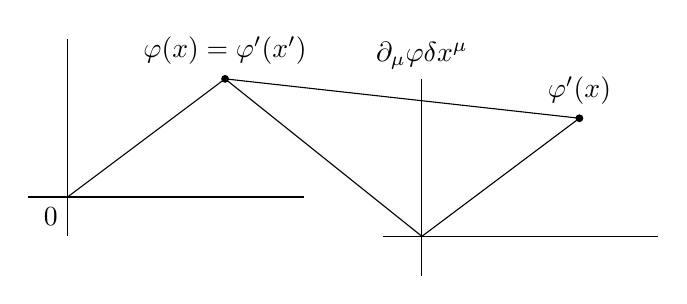
\begin{tikzpicture}
\draw (0,-.5) -- (0,2);
\draw (-.5,0) -- (3,0);
\draw (0,0) node[anchor=north east] {0};
\draw (0,0) -- (2,1.5) node[circle,fill,inner sep=1pt,label=above:{$\varphi(x)=\varphi'(x')$}]{};
\draw (4,-.5) -- (7.5,-.5);
\draw (4.5, -1) -- (4.5, 1.5) node[anchor=south]{$\partial_\mu\varphi\delta x^\mu$};
\draw (4.5,-.5) -- (6.5,1) node[circle,fill,inner sep=1pt,label=above:$\varphi'(x)$]{};
\draw (2,1.5) -- (4.5,-.5);
\draw (2,1.5) -- (6.5,1);
\end{tikzpicture}

\[ J^\mu_{(\nu)} = \pd{\mathcal{L}}{\partial_\mu\varphi}\partial_\rho\varphi - \eta^\mu_{\;\nu}\mathcal{L} \equiv \tilde{T}^\mu_{\;\nu} \]
\[ \tilde{T}^{\mu\nu} = \text{canonical energy-momentum tensor} \]
\[\begin{cases}
T^{\mu\nu} = \text{covariant EM tensor} \\
\tilde{T}^{\mu\nu} \text{is not symmetric $\mu\to\nu$}
\end{cases} \]

\[ Q_{(\nu)} \equiv \int \diff{^3x}\tilde{T}^{0}_{\;\nu} = \int \diff{^3x}\mathcal{P}_\nu \equiv P_\nu \]
 \[\begin{cases}
Q_{(0)} = \int \diff{^3x}\mathcal{P}_0 = \int \diff{^3x}\left(\pd{\mathcal{L}}{\partial_0\varphi}\partial_0\varphi - \mathcal{L}\right) \equiv \int \diff{^3x}\mathcal{H} = H \\
Q_{(i)} = \int \diff{^3x}\mathcal{P}_i = \int \diff{^3x}\pd{\mathcal{L}}{\partial_0\varphi}\partial_i\varphi
\end{cases}
\]

\subsubsection{Rotational invariance}
\[ \begin{cases}
x^{\prime\mu} = x^\mu + \omega^\mu_{\;\nu} x^\nu \\ \varphi'(x') = \varphi(x) - \frac{i}{2}\omega^{\mu\nu}\Omega_{\mu\nu}\varphi(x)
\end{cases} \qquad \to \qquad \begin{cases}
\delta x^\mu = \frac{1}{2}\omega^{\rho\sigma}\Xi^\mu_{(\rho\sigma)} \\ \delta \varphi = \frac{1}{2}\omega^{\rho\sigma}X_{(\rho\sigma)}
\end{cases} \]

\[ \begin{cases}
\Xi^\mu_{(\rho\sigma)} = \left(\eta^\mu_{\;\rho}\eta^\nu_{\;\sigma}-\eta^\mu_{\;\sigma}\eta^\nu_{\;\rho}\right)x^\rho \\
X_{(\rho\sigma)} = -i\Omega_{\rho\sigma}\varphi
\end{cases} \qquad \to \qquad \begin{cases}
\Omega_{\rho\sigma} = 0 \qquad (\text{scalar}) \\
\Omega_{\rho\sigma} = \Sigma'_{\rho\sigma} \qquad (\text{spinor})
\end{cases}\]

\[ J^\mu_{\rho\sigma} = \left(x_\rho\tilde{T}^\mu_\sigma - X_\sigma\tilde{T}^\mu_\rho\right) + S^\mu_{\rho\sigma} \]

\begin{align*}
Q_{(\rho\sigma)} &= \int \diff{^3x}J^0_{(\rho\sigma)} = \int \diff{^3x}\left[\left(x_\rho\mathcal{P}_\sigma - x_\sigma\mathcal{P}_\rho\right) + \mathcal{P}_{\rho\sigma}\right] \\
&= M_{\rho\sigma} = L_{\rho\sigma} + S_{\rho\sigma}
\end{align*}
Which is the external angular momentum plus the spin. ($x_\rho\mathcal{P}_\sigma - x_\sigma\mathcal{P}_\rho = \mathcal{L}_{\rho\sigma}$ and $\mathcal{P}_{\rho\sigma} = S^0_{\rho\sigma}$)

\section{Spin of a field}


\section{Dimensional analysis}
In the rest of part we set $c = 1 = \hbar $


\chapter{Canonical quantization}
It is now time to go from a classical to a quantum theory. This means quantization!
\section{Quantization}
\subsection{First quantization}
We start by exploring the quantization of a system with a finite number of degrees of freedom. We have already seen how to do this in the part on quantum mechanics. Here we give an alternative recipe (TODO: show that it is equivalent)
\[ \begin{cases}
p \equiv \pd{L}{\dot{q}} \\
H = p \; \dot{q} - L
\end{cases} \]
The equations of motion are given by the Poisson brackets
\[ \begin{cases}
\left\{q_i,p_j\right\}_t = \delta_{ij} \\ \left\{q_i,q_j\right\} = 0 = \left\{p_i,p_j\right\}
\end{cases} \qquad \begin{cases}
\dot{q}_i = \left\{q_i,H\right\}_t \\ \dot{p}_i = \left\{p_i, H\right\}_t
\end{cases}\]
We obtain the canonical quantization by applying the following substitutions:
\begin{itemize}
\item $(q_i, p_i)$ which are variables become $(X_i,P_i)$ which are operators;
\item $\{\;,\;\}_t \qquad \to \qquad - \frac{i}{\hbar}[\;,\;]_t$.
\end{itemize}
This gives us the following equations:
\[ \begin{cases}
[X_i,P_j]_t = i\hbar\delta_{ij} \\ [X_i,X_j] = 0 = [P_i,P_j]
\end{cases} \qquad \begin{cases}
\od{X_i}{t}  = - \frac{i}{\hbar}[X_i,H] \\ \od{P_i}{t} = - \frac{i}{\hbar}[P_i, H]
\end{cases} \]
As we can see, the operators evolve, so these are equations of motion in the Heisenberg picture.


For a finite number of degrees of freedom in momentum space we have $N$ independent oscillators.
\[ \begin{cases}
[a_p,a^\dagger_k] = \delta_{pk} \\
[a_p,a_k] = 0 = [a^\dagger_p, a^\dagger_k]
\end{cases} \]

(90\% of physics is harmonic oscillators because we expand to second order)



\subsection{Second quantization}
This procedure generalises quite nicely to fields with infinite degrees of freedom.
\[ \begin{cases}
\pi(x) \equiv \pd{\mathcal{L}}{\partial_0\varphi} \\ \mathcal{H} = \pi\cdot\partial_0\varphi - \mathcal{L}
\end{cases} \]
The Poisson brackets:
\[ \begin{cases}
\left\{\varphi(\overline{x},t),\pi(\overline{y},t)\right\}_t = \delta^3(\overline{x}- \overline{y}) \\ \left\{\varphi(\overline{x},t),\varphi(\overline{y},t)\right\}_t = 0 = \left\{\pi(\overline{x},t),\pi(\overline{y},t)\right\}_t
\end{cases} \qquad \begin{cases}
\dot{\varphi}(\overline{x},t) = \left\{\varphi(\overline{x},t),H\right\}_t \\ \dot{\pi}(\overline{x},t) = \left\{\pi(\overline{x},t), H\right\}_t
\end{cases}\]
The quantization given by following substitution:
\begin{itemize}
\item $(\varphi, \pi)$ = classical fields $\to$ $(\hat{\varphi}, \hat{\pi})$ = operator fields
\item $\{\;,\;\}_t \qquad \to \qquad -i[\;,\;]_t \qquad (\hbar = 1 =c)$
\end{itemize}
This gives us the following quantization:
\[ \begin{cases}
\left[\hat{\varphi}(\overline{x},t), \hat{\pi}(\overline{y},t)\right]_t = i\delta^3(\overline{x}- \overline{y}) \\
\left[\hat{\varphi}(\overline{x},t)\hat{\varphi}(\overline{y},t)\right]_t = 0 = \left[\hat{\pi}(\overline{x},t), \hat{\pi}(\overline{y},t)\right]_t
\end{cases} \qquad \begin{cases}
\dot{\hat{\varphi}}(\overline{x},t) = -i \left[\hat{\varphi}(\overline{x},t), \hat{H}\right]_t \\
\dot{\hat{\pi}}(\overline{x},t) = -i \left[\hat{\pi}(\overline{x},t), \hat{H}\right]_t
\end{cases}\]



In momentum space we get an equivalent quantization condition:
\[ \begin{cases}
\left[a(p), a^\dagger(k)\right] = \delta^3(\vec{p}- \vec{k}) \\
\left[a(p),a(k)\right] = 0 = \left[a^\dagger(p), a^\dagger(k)\right]
\end{cases} \]
Which is a continuous set of uncoupled harmonic oscillators.

\section{Number (density) operator}
TODO see p5-6 in Mandl-Shaw

The \udef{number density operator}
\[ \mathcal{N}(k) \equiv a^\dagger(k)a(k)\]
has the following properties

\begin{eigenschap}
\begin{itemize}
\item  $\mathcal{N}(k)^\dagger = \mathcal{N}(k)$
\item \raisebox{-0.95em}{$\begin{aligned}
&[\mathcal{N}(k), a(p)] = -a(p)\delta^3(\overline{k}- \overline{p}) \\
&[\mathcal{N}(k), a^\dagger(p)] = +a^\dagger(p)\delta^3(\overline{k}- \overline{p})
\end{aligned}$}
\end{itemize}
\end{eigenschap}


The \udef{number operator}
\[ N \equiv \int \diff{^3k}\mathcal{N}(k)\]
has the following properties
\begin{eigenschap}
\begin{itemize}
\item  $N^\dagger = N$
\item \raisebox{-0.95em}{$\begin{aligned}
&[N, a(p)] = -a(p) \\
&[N, a^\dagger(p)] = +a(p)
\end{aligned}$}
\end{itemize}
\end{eigenschap}

\section{Normal ordering}

\section{What are the states in QFT?}
So far we have operator fields, but no states. The space of states in quantum field theory is called the \udef{Fock Space}.
\subsection{Postulate of the existence of vacuum $=\ket{0}$}
\[ \boxed{a(k)\ket{0}=0} \qquad \forall k \]
\[ \begin{cases}
\mathcal{N}(k)\ket{0} = 0 \qquad \to \qquad 0\; \text{occupation number} \\
N[H]\ket{0} = 0 \qquad \to \qquad 0\; \text{energy, momentum}
\end{cases} \]

\subsection{The Fock space}(Hilbert space) is the space with \ueig{all possible states} generated by applying $a^\dagger(k)$ on $\ket{0}$. So a generic state in Fock space can be written as
\[ \ket{n_1(k_1), \ldots, n_l(k_l)}\quad \sim \quad a^\dagger(k_1)^{n_1} \ldots a^\dagger(k_l)^{n_l} \ket{0} \]

\begin{example}
We consider the simplest non vacuum state $\ket{1(k)} \sim a^\dagger(k)\ket{0}$.
\begin{align*}
N\ket{1(k)} &\sim \int \diff{^3p}\mathcal{N}(p)a^\dagger(k)\ket{0} \\
&= \int \diff{^3p}\left([\mathcal{N}(p),a^\dagger(k)] + a^\dagger(k)\mathcal{N}(p)\right)\ket{0} \\
&= \int \diff{^3p} \delta^3(k-p)a^\dagger(k)\ket{0} + \cancel{a^\dagger(p)\mathcal{N}(k)\ket{0}} \\
&= \int \diff{^3p} \left(1\delta^3(k- p)a^\dagger(p) + \cancel{a^\dagger(p)\mathcal{N}(k)}\right)\ket{0} \\
&\sim +1 \ket{1(k)}
\end{align*}
Similarly
\[ \begin{cases}
H\ket{1(k)} = \omega_k\ket{1(k)} \qquad \text{where} \qquad \omega_k = \left(m^2 + |\overline{k}|^2\right)^{1/2} \\
P\ket{1(k)} = k\ket{1(k)}
\end{cases} \]
From this we get for a state of $n$ identical particles
\begin{align*}
\ket{n(k)} &\sim a^\dagger(k)^n\ket{0}\\
N\ket{n(k)} &= n\ket{n(k)} \\
H\ket{n(k)} &= n\omega_k\ket{n(k)}\\
\overline{P}\ket{n(k)} &= n \overline{k} \ket{n(k)}
\end{align*}
Also
\begin{align*}
\ket{n_1(k_1), n_2(k_2)} &\sim a^\dagger(k_1)^{n_1}a^\dagger(k_2)^{n_2}\ket{0}\\
N\ket{n_1(k_1), n_2(k_2)} &= (n_1+n_2)\ket{n_1(k_1), n_2(k_2)} \\
H\ket{n_1(k_1), n_2(k_2)} &= (n_1\omega_1+n_2\omega_2)\ket{n_1(k_1), n_2(k_2)} \\
P\ket{n_1(k_1), n_2(k_2)} &= (n_1k_1+n_2k_2)\ket{n_1(k_1), n_2(k_2)}
\end{align*}
\end{example}

From this example we learn that the Fock space of a real scalar field corresponds to a particle with Bose statistics, as we can add as many identical particles as we want.
\begin{eigenschap}
Scalar field corresponds to spin 0
\end{eigenschap}

\subsection{Normalization of states}
\[ \braket{1(p)}{1(k)} = \delta^3(\overline{k}- \overline{p}) \]


Firstly
\[\braket{0}{0} = 1\]
Normally we would normalize the states as follows
\[ \begin{cases}
\ket{1(k)} = a^\dagger(k)\ket{0} \\
\braket{1(p)}{1(k)} = \delta^3(\overline{k}- \overline{p})
\end{cases}\]
This normalisation is not invariant under Lorentz transformations however.

So we use the ``good'' normalization
\[ \begin{cases}
\ket{1(k)} = (2\pi)^{3/2}\sqrt{2\omega_k}a^\dagger(k)\ket{0} \\
\braket{1(p)}{1(k)} = (2\pi)^{3}2\omega_k\delta^3(\overline{k}- \overline{p})
\end{cases} \]

\section{Covariant commutators and propagators}
\subsection{Feynman propagator}

\begin{definition}
The \udef{Feynman propagator} $\Delta_F$ is defined as
\[ \Delta_F(x-y) \equiv \expval{T \left(\varphi(x)\varphi(y)\right)}{0} = \varphi(x)\varphi(y) \]
\end{definition}
\begin{align*}
\Delta_F(x-y) &= \theta(x_0-y_0)\expval{T \left(\varphi(x)\varphi(y)\right)}{0} + \theta(y_0-x_0)\expval{T \left(\varphi(x)\varphi(y)\right)}{0} \\
&= \theta(x_0-y_0)\expval{T \left(\varphi_+(x)\varphi_-(y)\right)}{0} + \theta(y_0-x_0)\expval{T \left(\varphi_+(x)\varphi_-(y)\right)}{0} \\
&= \theta(x_0-y_0)\expval{[\varphi_+(x), \varphi_-(y)]}{0} - \theta(y_0-x_0)\expval{[\varphi_-(x), \varphi_+(y)]}{0} \\
&= \theta(x_0-y_0)D_+(x-y) - \theta(y_0-x_0)D_-(x-y)
\end{align*}
The following relation holds
\[ T \left(\varphi(x)\varphi(y)\right) = N\left(\varphi(x)\varphi(y)\right) + \varphi(x)\varphi(y)  \]
\begin{align*}
\varphi(x)\varphi(y) = T\left(\varphi(x)\varphi(y)\right) - N\left(\varphi(x)\varphi(y)\right) \\
&= \theta(x_0-y_0)\left(\cancel{\varphi_-(x)\varphi_-(y)}+\xcancel{\varphi_+(x)\varphi_+(y)}+\bcancel{\varphi_-(x)\varphi_+(y)}+\varphi_+(x)\varphi_-(y)\right) + \theta(y_0-x_0)\left(\cancel{\varphi_-(y)\varphi_-(x)}+\xcancel{\varphi_+(y)\varphi_+(x)}+\varphi_+(y)\varphi_-(x)+\bcancel{\varphi_-(y)\varphi_+(x)}\right) \\
- \theta(x_0-y_0)\left(\cancel{\varphi_-(x)\varphi_-(y)}+\xcancel{\varphi_+(x)\varphi_+(y)}+\bcancel{\varphi_-(x)\varphi_+(y)}+\varphi_-(y)\varphi_+(x)\right) - \theta(y_0-x_0)\left(\cancel{\varphi_-(x)\varphi_-(y)}+\xcancel{\varphi_+(x)\varphi_+(y)}+\varphi_-(x)\varphi_+(y)+\bcancel{\varphi_-(y)\varphi_+(x)}\right)
&= \theta(x_0 - y_0)\left[\varphi_+(x),\varphi_-(y)\right] - \theta(y_0-x_0)\left[\varphi_-(x),\varphi_+(y)\right] \\
&= \theta(x_0 - y_0)D_+(x-y) - \theta(y_0-x_0)D_-(x-y)
\end{align*}


\begin{definition}
The \udef{Feynman propagator} (complex scalar)
\begin{align*}
\Delta_F(x-y) &\equiv \expval{T \left(\varphi(x)\varphi^\dagger(y)\right)}{0} = \underbrace{\varphi(x)\varphi^\dagger(y)} \\
&= \theta(x_0-y_0)D_+(x-y) - \theta(y_0-x_0)D_-(x-y)
\end{align*}
\end{definition}

\begin{definition}
The \udef{Feynman propagator for Dirac fields}
\begin{align*}
S^{\alpha\beta}_+(x-y) &\equiv \expval{T \left(\psi_{\alpha}(x)\overline{\psi}_{\beta}(y)\right)}{0} = \underbrace{\psi_{\alpha}(x)\overline{\psi}_{\beta}(y)} \\
&= \theta(x_0-y_0)S_+^{\alpha\beta}(x-y) - \theta(y_0-x_0)S^{\alpha\beta}_-(x-y) \\
&= (i\slashed{\partial}+m)D_F(x-y)
\end{align*}
\remark{Ex.}
\end{definition}


\subsection{Time-ordered product}
\begin{definition}
The \udef{time-ordered product} of two operators $A$ and $B$
\[ T \left(A(t_1)B(t_2)\right) = \begin{cases}
A(t_1)B(t_2) & (t_1 > t_2) \\
\pm B(t_2)A(t_1) & (t_1 < t_2)
\end{cases} \]
Where the $\pm$ is $+$ for bosons and $-$ for fermions. For $n$ operators, the time-ordered product orders them by time and introduces a factor $(-1)^p$ where $p$ is the number of fermionic exchanges necessary to achieve time ordering.

The time-ordered product is also taken to be linear, if addition were to turn up in the product.
\end{definition}

\subsection{Introducing Feynman diagrams}
integral over time, no time ordering. time left to right. arrows and momenta

\subsection{Microcausality}

\section{Spin statistics theorem}
\subsection{Quantization with anti-commutators}

\chapter{Some examples of quantum field theories}
We want an explicit expression for the Lagrangian density. We will try to guess its form.
\begin{enumerate}
\item The action is more or less an observable so we want it to be real (Hermitian)
\remark{$\mathcal{L} = $ real (Hermitian)}
\item The action is a scalar (under Poincaré transformation)
\remark{$\mathcal{L} = $ scalar density}
\item The action is adimensional in natural units
\[ \hookrightarrow S = \int \diff{^4x}\mathcal{L} = [M]^{-4}[M]^4 = [M]^0 \]
\item By equation of motion $\to$ relativistic equation = nice
\[ \mathcal{L}(\varphi, \partial_\mu\varphi) \]
\end{enumerate}


\section{Klein-Gordon field (real scalar field)}


As a first example, we consider the following Lagrangian for a real scalar field:
\[ \mathcal{L} = \frac{1}{2}(\partial_\mu\varphi)(\partial^\mu\varphi) - \frac{1}{2}m^2\varphi^2 \]
where $m$ is a parameter that we will identify with the mass.
This can be seen as the sum of kinetic and a mass term (TODO why?). Knowing that the Lagrangian must have a dimension of $[M^4]$ and that each derivative has dimension $[\partial] = [M^1]$, we see that
\[ \begin{cases}
[\varphi] = [M^1] \\
[m] = [M^1]
\end{cases} \]
Luckily this is consistent with our identification of $m$ as the mass.

Because we are dealing with a real and relativistic field, we impose the following conditions
\[ \begin{cases}
\varphi(x) = \varphi^*(x) \\
\varphi'(x') = \varphi(x)
\end{cases} \]
where the prime means the quantity has been transformed by a Poincaré transformation.

\subsection{Equation of motion}
Applying the Euler-Lagrange equation
\[ \pd{\mathcal{L}}{\varphi} - \partial_\mu \pd{\mathcal{L}}{\partial_\mu\varphi} = 0 \]
We get the Klein-Gordon equation:
\[ -m^2\varphi - \partial_\mu\partial^\mu\varphi = -(\Box+m^2)\varphi = 0\]
As we know this has the following general solution:
\[ \varphi(x) = \frac{1}{(2\pi)^{3/2}}\int \diff{^3k}\left(a(k)e^{-ikx} + a^*(k)e^{ikx}\right)_{k_0 = \omega_k} \]

\subsection{Hamiltonian formulation}
We now calculate the relevant quantities in the Hamiltonian formulation.
\[ \pi \equiv \pd{\mathcal{L}}{\partial_0\varphi} = \frac{1}{2}(\partial_0 \varphi + \partial^0 \varphi) = \partial_0 \varphi \]
\[ \mathcal{H} = \pi \partial_0\varphi - \mathcal{L} = \frac{1}{2}\pi^2 + \frac{1}{2}(\overline{\nabla}\varphi)^2 + \frac{1}{2}m^2\varphi^2 \]
We see that the Hamiltonian density is always positive. (TODO: as opposed to ...)
\[ H = \int \diff{^3x}\mathcal{H} > 0 \]

\begin{example}
Exercise: Verify Poisson Brackets
\begin{align*}
\dot{\varphi} &= \left\{\varphi(\overline{x},t), H\right\}_t \\
\dot{\pi} &= \left\{\pi(\overline{x},t), H\right\}_t
\end{align*}
\[ \left\{\varphi(\overline{x},t), \varphi(\overline{y},t)\right\} = 0 \]
\end{example}

\subsection{Symmetries}
\subsubsection{Translational invariance}
\[J^\mu_{(\nu)} = (\partial^\mu\varphi)(\partial_\nu\varphi) - \eta^\mu_{\;\nu}\mathcal{L}\]
\[ \partial_\mu J^\mu_{(\nu)} = 0 \qquad \to \qquad \text{Exercise: prove} \]
The 4 conserved charges:
\[\begin{cases}
P_0 \equiv H = \int \diff{^3x}\left\{\pi\partial_0\varphi-\mathcal{L}\right\} = \int \diff{^3x}\mathcal{H} \\
P_i = \int \diff{^3x}\mathcal{P}_i = \int \diff{^3x} \pi(\partial_i\varphi)
\end{cases}\]

\subsubsection{Rotational invariance}

\[\begin{cases}
\delta x^\mu = \omega^{\rho\sigma}\Xi^\mu_{(\rho\sigma)} \qquad \to \qquad \Xi^\mu_{(\rho\sigma)} = \left(\eta^\mu_{\;\rho}\eta^\nu_{\;\sigma}-\eta^\mu_{\;\sigma}\eta^\nu_{\;\rho}\right)x^\nu \\
\delta \varphi = \frac{1}{2}\omega^{\rho\sigma}X_{(\rho\sigma)} = 0 \qquad \to \qquad X_{(\rho\sigma)} = 0
\end{cases} \]
Differences??
\[ \frac{1}{2},\nu \text{ipv} \rho \]

\[ J^\mu_{(\rho\sigma)} = \left(x_\rho\tilde{T}^\mu_{\;\sigma} - x_\sigma\tilde{T}^\mu_{\;\rho}\right) + (X) \]

\begin{align*}
Q_{(\rho\sigma)} &= \int \diff{^3x}J^0_{(\rho\sigma)} = \int \diff{^3x}\left(x_\rho\mathcal{P}_\sigma - x_\sigma\mathcal{P}_\rho\right) =L_{(\sigma\rho)??\text{(last equality)}}
\end{align*}

\begin{example}
Exercise: Write $P^\mu$ in the momentum space (as functions of $a(k), a^*(k)$)

Solution:
\[\varphi(x) = \frac{1}{(2\pi)^{3/2}}\int \frac{\diff{^3k}}{\sqrt{2\omega_k}}\left(a(k)e^{-ikx}+a^*(k)e^{ikx}\right)_{k_0 = \omega_k} \]
\begin{align*}
H &= \frac{1}{2} \int \diff{^3x}\left(\pi^2 + (\overline{\nabla})^2 m^2\varphi^2\right) \\
&= \frac{1}{2}\int \frac{\diff{^3x}}{(2\pi)^3}\int \frac{\diff{^3k}\diff{^3p}}{\sqrt{4\omega_k\omega_p-\omega_k}} \times \left\{(-i\omega_k)(-i\omega_p)\left[a(k)a(p)e^{-i(k+p)x}+a^*(k)a^*(p)e^{i(k+p)x}-a(k)a^*(p)e^{-i(k-p)x}-a^*(k)a(p)e^{i(k-p)x}\right] + (i \overline{k})(i \overline{p})\left[a(k)a(p)e^{-i(k+p)x}+a^*(k)a^*(p)e^{i(k+p)x}-a(k)a^*(p)e^{-i(k-p)x}-a^*(k)a(p)e^{i(k-p)x}\right] + m^2 \left[a(k)a(p)e^{-i(k+p)x}+a^*(k)a^*(p)e^{i(k+p)x}-a(k)a^*(p)e^{-i(k-p)x}-a^*(k)a(p)e^{i(k-p)x}\right] \right\} \\
&= \frac{1}{2} \int \frac{\diff{^3k}\diff{^3p}}{\sqrt{4\omega_k\omega_p-\omega_k}}
\int \frac{\diff{^3x}}{(2\pi)^3} \left\{(m^2-\omega_k\omega_k - \overline{k}\cdot\overline{p})
\left[a(k)a(p)e^{-i(k+p)x}+a^*(k)a^*(p)e^{i(k+p)x}\right]
+ \left[a(k)a^*(p)e^{-i(k-p)x}+a^*(k)a(p)e^{i(k-p)x}\right] \right\}
\end{align*}
Let's integrate $\int \diff{^3x}$:
\[H = \frac{1}{2}\int \frac{\diff{^3k}\diff{^3p}}{\sqrt{4\omega_k\omega_p}} \left\{ \delta^3(\overline{k}+\overline{p})(m^2-\omega_k\omega_p - \overline{k}\cdot \overline{p})\left[ a(k)a(p)e^{-i(k_0+p_0)x_0} + a^*(k)a^*(p)e^{+i(k_0+p_0)x_0} \right] + \delta^3(\overline{k}-\overline{p})(m^2+\omega_k\omega_p + \overline{k}\cdot \overline{p})\left[ a(k)a^*(p)e^{-i(k_0-p_0)x_0} + a^*(k)a(p)e^{+i(k_0-p_0)x_0} \right] \right\}\]
Let's integrate $\int \diff{^3p}$:
\begin{align*}
H &= \frac{1}{2}\int \frac{\diff{^3k}}{2\omega_k} \left\{ (m^2-\omega_k^2 - |\overline{k}|^2)\left[ \ldots \right] + (m^2+\omega_k^2 + |\overline{k}|^2)\left[ a(k)a^*(p) + a^*(k)a(p) \right] \right\} \\
&=\frac{1}{2} \int \diff{^3k}\omega_k(a(k)a^*(k)+a^*(k)a(k))
\end{align*}
We didn't use any ``commutator property''
\[ \boxed{H = \int \diff{^3k}\omega_ka^*(k)a(k)} \qquad \text{total energy} \]
\begin{align*}
P^i &= \int \diff{^3k} k^i(a(k)a^*(k) + a^*(k)a(k)) \\
\Aboxed{P^i &= \int \diff{^3 k}k^ia^*(k)a(k)} \qquad \text{total free momentum}
\end{align*}

\end{example}

\subsection{Quantization}

Following the recipe for the second quantization (TODO ref), we get
\[ \begin{cases}
\left[\hat{\varphi}(\vec{x},t), \hat{\pi}(\vec{y},t)\right]_t = i\delta^3(\vec{x}- \vec{y}) \\
\left[\hat{\varphi}(\vec{x},t)\hat{\varphi}(\vec{y},t)\right]_t = 0 = \left[\hat{\pi}(\vec{x},t), \hat{\pi}(\vec{y},t)\right]_t
\end{cases} \]

We have already shown that the solutions of the Klein-Gordon equation are of the form 
\[ \begin{cases}
\hat{\varphi}(x) = \frac{1}{(2\pi)^{3/2}} \int \frac{\diff{^3k}}{\sqrt{2\omega_k}} \left(\hat{a}(k)e^{-ikx} + \hat{a}^\dagger(k)e^{ikx}\right)_{k_o=\omega_k} \\
\hat{\pi}(x) = \frac{-i}{(2\pi)^{3/2}} \int \frac{\diff{^3k}}{\sqrt{2\omega_k}} \omega_k \left(\hat{a}(k)e^{-ikx} - \hat{a}^\dagger(k)e^{ikx}\right)_{k_o=\omega_k}
\end{cases} \]
where the integral is over all wave vectors allowed by the boundary conditions.
Alternatively, we can write in momentum space
\[ \begin{cases}
\hat{a}(p) = \left. \frac{1}{(2\pi)^{3/2}} \int \frac{\diff{^3x}}{\sqrt{2\omega_p}} \left(\omega_p\varphi(\vec{x},t)+i\pi(\vec{x},t)\right)e^{ipx}\right|_{p_o=\omega_p} \\
\hat{a}^\dagger(p) = \left. \frac{1}{(2\pi)^{3/2}} \int \frac{\diff{^3x}}{\sqrt{2\omega_p}} \left(\omega_p\varphi(\vec{x},t)-i\pi(\vec{x},t)\right)e^{-ipx}\right|_{p_o=\omega_p}
\end{cases} \]

In momentum space we get an equivalent quantization condition:
\[ \begin{cases}
\left[a(p), a^\dagger(k)\right] = \delta^3(\vec{p}- \vec{k}) \\
\left[a(p),a(k)\right] = 0 = \left[a^\dagger(p), a^\dagger(k)\right]
\end{cases} \]
These are the harmonic oscillator commutation relations for a continuous set of uncoupled harmonic oscillators.


\subsection{Hamiltonian (density)}
The \udef{Hamiltonian density operator}
\[ \mathcal{H}(\varphi, \pi) \equiv \frac{1}{2}\pi^2 + \frac{1}{2}(\overline{\nabla}\varphi)^2 + \frac{1}{2}m^2\varphi^2 \]
The \udef{Hamiltonian operator}
\begin{align*}
H &= \int \diff{^3x}\mathcal{H} = \frac{1}{2}\int\diff{^3k}\omega_k \left(a^\dagger(k)a(k) + a(k)a^\dagger(k)\right) \\
&= \int\diff{^3k}\omega_k \left(a^\dagger(k)a(k) + \frac{1}{2}[a(k),a^\dagger(k)]\right) \\
&= \underbrace{\int \diff{^3k}\omega_k\mathcal{N}(k)}_{\Delta E \text{energy operator}} + \xcancel{\frac{1}{2}\int \diff{^3k}\omega_k\delta^3(\overline{k}- \overline{k})}
\end{align*}
\[ N[H] = \int \diff{^3k}\omega_k\mathcal{N}(k) \]

The dropped term corresponds to the constant energy of vacuum ($E_0 \;\to\; \infty$). We drop it here because it is constant (i.e. a number, not an operator), but it becomes relevant when quantizing gravity.

\subsection{Three momentum (density) operator}
\begin{align*}
P_i &= \int \diff{^3x}\pi(\partial_i\varphi) = \ldots \\
&= \frac{1}{2}\int \diff{^3k}(k_i)\left(a^\dagger(k)a(k)+ a(k)a^\dagger(k)\right) \\
&= \int \diff{^3k} k_i \mathcal{N}(k) + \xcancel{\infty -\text{number}}
\end{align*}
\[ N[P_i] = \int \diff{^3k} k_i \mathcal{N}(k) \]

The switching round of $a(k)$ and $a^\dagger(k)$ in the previous calculations motivates us to make the following definition:
\begin{definition}
A product is \udef{normal ordered} when all creation operators are to the left of all annihilation operators in the product. I.e. when all $a^\dagger$ are on the left and all $a(k)$ are on the right
\[ N[a^\dagger(k)a(k) + a(k)a^\dagger(k)] = 2 a^\dagger(k)a(k) \]
Inside $N[\;]$ (for scalar fields) everything commutes.
\end{definition}
\remark{Normal ordering does not touch any H.O. commutators}

\subsection{General solution and interpretation}


From now on we drop the hats over the operators to make the notation less heavy. We also split 
\begin{align*}
\varphi(x) &= \frac{1}{(2\pi)^{3/2}} \int \frac{\diff{^{3}k}}{\sqrt{2\omega_k}}\left(a(k)e^{-ikx} + a^\dagger(k)e^{ikx}\right)_{k_0 = \omega_k} \\
&= \varphi_+(x) + \varphi_-(x)
\end{align*}
The operators $\varphi_\pm(x)$ are the annihilation / creation operators of a particle with only momentum $k$ at the point $x$.

One-particle states are linear superpositions of
\[ a^\dagger(\vec{k})\ket{0} \qquad\text{for any}\qquad \vec{k} \]
Two-particle states are linear superpositions of
\[ a^\dagger(\vec{k})a^\dagger(\vec{k'})\ket{0} \qquad\text{for any}\qquad  \vec{k}, \vec{k'} \neq \vec{k} \]
and
\[ \frac{1}{\sqrt{2}}(a^\dagger(\vec{k}))^2\ket{0} \qquad\text{for any}\qquad  \vec{k} \]

These states are normalized if the vacuum state is normalized.
\begin{example}
\begin{align*}
\bra{0}\left(\varphi_+(x)\ket{1(p)}\right) &= \frac{1}{(2\pi)^{3/2}} \int \frac{\diff{^{3}k}}{\sqrt{2\omega_k}}(2\pi)^{3/2}\sqrt{2\omega_p}\braket[a(k)a^\dagger(p)]{0}{0}e^{-ikx} \\
&= \int \diff{^3k}\frac{\sqrt{2\omega_p}}{\sqrt{2\omega_k}}\delta^3(\overline{k} - \overline{p})e^{-ikx}\braket{0}{0} = e^{-ipx}
\end{align*}
\end{example}
(This example also hints at the reason why the ``good'' normalization is good)


\subsection{Covariant commutators}
So far the story has been:
\begin{enumerate}
\item We defined the Lagrangian density, $\mathcal{L}$, which is a \ueig{covariant} object.
\item We then switched to the Hamiltonian formalism, with $\mathcal{H} = \pi\partial_0\varphi - \mathcal{L}$. This is the Legendre transformation of the Lagrangian density. The Hamiltonian density $\mathcal{H}$ is not manifestly covariant. (Which is why we stressed that we compute it at fixed time)
\item We then applied the canonical quantization to get $[\varphi(\overline{x},t), \pi(\overline{y},t)] = i\delta^3(\overline{x}- \overline{y})$, which is not manifestly covariant.
\end{enumerate}
So we need now to verify that the canonical quantization is consistent with Lorentz covariance.
In other words, we need to show that the commutation relations are covariant. 
To do that, we write the commutator $[\varphi(x), \varphi(y)]$ for two arbitrary spacetime points $x$ and $y$.

First we note that
\[ [\varphi_+(x),\varphi_+(y)] = [\varphi_-(x),\varphi_-(y)] = 0. \]
So
\begin{align*}
[\varphi(x), \varphi(y)] &= [\varphi_+(x)+\varphi_-(x), \varphi_+(y) + \varphi_-(y)] \\
&= [\varphi_+(x), \varphi_-(y)] + [\varphi_-(x), \varphi_+(y)] \\
&\equiv D_+(x,y) + D_-(x,y)
\end{align*}
Working out each part separately, we get
\begin{align*}
D_+(x,y) &\equiv [\varphi_+(x), \varphi_-(y)]\\
&= \frac{1}{(2\pi)^{3}} \int \frac{\diff{^{3}k}}{\sqrt{2\omega_k}} \int \frac{\diff{^{3}k'}}{\sqrt{2\omega_{k'}}} e^{-ikx}e^{ik'y}\left[a(k), a^\dagger(k')\right] \\
&= \left.\frac{1}{(2\pi)^{3}} \int \frac{\diff{^{3}k}}{2\omega_k} e^{-ik(x-y)}\right|_{k_0 = \omega_k}
\end{align*}
and
\begin{align*}
D_-(x,y) &\equiv [\varphi_-(x), \varphi_+(y)]\\
&= \frac{1}{(2\pi)^{3}} \int \frac{\diff{^{3}k}}{\sqrt{2\omega_k}} \int \frac{\diff{^{3}k'}}{\sqrt{2\omega_{k'}}} e^{ikx}e^{-ik'y}\left[a^\dagger(k), a(k')\right] \\
&= -\left.\frac{1}{(2\pi)^{3}} \int \frac{\diff{^{3}k}}{2\omega_k} e^{ik(x-y)}\right|_{k_0 = \omega_k}
\end{align*}
We notice that $D_+$ and $D_-$ do not really depend on both $x$ and $y$, but rather on their difference $x-y$. Thus we can define
\begin{align*}
D(x-y) &\equiv D_+(x-y) + D_-(x-y) \\
&= \left.\frac{1}{(2\pi)^3}\int \frac{\diff{^3k}}{2\omega_k}\left( e^{-ik(x-y)} - e^{ik(x-y)} \right)\right|_{k_0=\omega_k} \\
&= - \left.\frac{1}{(2\pi)^3}\int \frac{\diff{^3k}}{\omega_k}\sinh(x-y)\right|_{k_0=\omega_k}
\end{align*}


We can now write $D_\pm(x-y)$ in a covariant way:
\[ D_\pm(x-y) \equiv i \int_{c_\pm}\frac{\diff{^4k}}{(2\pi)^4}\frac{e^{-ik(x-y)}}{k^2-m^2} \]



Let's calculate $D_+(x-y)$
\begin{align*}
D_+(x-y) &= \frac{i}{(2\pi)^4}\int_{c_+}\diff{^4k}\frac{e^{-ik(x-y)}}{k^2-m^2} \\
&= i \int \frac{\diff{^3k}}{(2\pi)^3}e^{i \overline{k}(\overline{x}- \overline{y})} \cdot \int_{c_+} \frac{\diff{k_0}}{2\pi} \frac{e^{ik_0(x_0-y_0)}}{(k_0-\omega_k)(k_0+\omega_k)}
\end{align*}
We define
\[ f(k_0) = \frac{e^{ik_0(x_0-y_0)}}{2\pi(k_0-\omega_k)(k_0+\omega_k)} \]
Now, using the residue theorem
\begin{eigenschap}
\ueig{Residue theorem}
\[ \int_{c_+}\diff{k_0}f(k_0) = -2\pi i \Res(f(k_0))_{k_0=\omega_k} \]
\end{eigenschap}

\begin{figure}
\centering
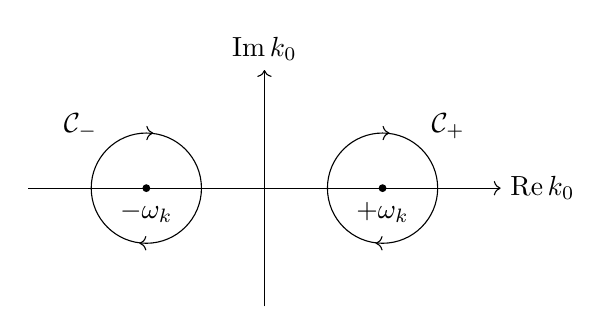
\begin{tikzpicture}
\draw[->] (-3,0) -- (3,0) node[anchor=west]{$\text{Re}\,k_0$};
\draw[->] (0,-1.5) -- (0,1.5) node[anchor=south]{$\text{Im}\,k_0$};
\draw (-1.5,0) node[circle,fill,inner sep=1pt, label=below:$-\omega_k$]{};
\draw (1.5,0) node[circle,fill,inner sep=1pt, label=below:$+\omega_k$]{};
\draw[decoration={markings, mark=at position 0.25 with {\arrow{<}}, markings, mark=at position 0.75 with {\arrow{<}}}, postaction={decorate}] (-1.5,0) circle (.7);
\draw[decoration={markings, mark=at position 0.25 with {\arrow{<}}, markings, mark=at position 0.75 with {\arrow{<}}}, postaction={decorate}] (1.5,0) circle (.7);
\draw (2,.5) node[anchor=south west] {$\mathcal{C}_+$};
\draw (-2,.5) node[anchor=south east] {$\mathcal{C}_-$};
\end{tikzpicture}
\end{figure}

we get
\[D_+(x-y) = i \int \frac{\diff{^3k}}{(2\pi)^3}(-2\pi i) \frac{e^{-i\omega_k(x_0-y_0)}}{(2\pi)2\omega_k}e^{i \overline{k}(\overline{x} - \overline{y})} = \left.\frac{1}{(2\pi)^3}e^{-ik(x-y)}\right|_{k_0=\omega_k} \]

In conclusion the quantization conditions are consistent with covariance of the theory
\[ D(x-y) = [\varphi(x), \varphi(y)] \]
\begin{example}
Exercise: $[\pi(x), \pi(y)], [\varphi(x), \pi(y)]$
\end{example}

\subsection{Covariance and causality}
\begin{itemize}
\item $D(x-y) \equiv [\varphi(x),\varphi(y)]$ is covariant.
\item $\left.D(x-y)\right|_{x_0=y_0} = [\varphi(x,t), \varphi(y,t)] = 0$

So $D(x-y) = 0$ if $(x-y)^2<0$ (space line)
\end{itemize}

The creation / annihilation of a particle $(x_0, \overline{x})$ cannot be influenced by the creation / annihilation of a particle $(y_0,\overline{y})$ if $(x-y)^2<0$

Given $A,B$; if $[A,B] = 0$ there is no interference in the measurement

Microcausality.

Lecture 5/11

Recap
Canonical quantization of complex scalar (free)
\begin{enumerate}
\item General form
\begin{align*}
\varphi(x) = \frac{1}{(2\pi)^{3/2}} \int \frac{\diff{^3k}}{2\omega_k}() \equiv \varphi_+(x)+\varphi_-(x)\\
\end{align*}
?
\item Hamiltonian formalism
\begin{align*}
\pi &\equiv \pd{\mathcal{L}}{\partial_0\varphi} = \partial_0\varphi^\dagger \qquad \to \qquad (\varphi, \pi) \\
\pi^\dagger &\equiv \pd{\mathcal{L}}{\partial_0\varphi^\dagger} = \partial_0\varphi \qquad \to \qquad (\varphi^\dagger, \pi^\dagger)
\end{align*}
\[\mathcal{H} = \pi\partial_0\varphi + \pi^\dagger\partial_0\varphi^\dagger - \mathcal{L}\]
\item Canonical quantization
\begin{align*}
[\varphi(\overline{x},t), \pi(\overline{y},t)]_t &= i\delta^3(\overline{x}- \overline{y}) = [\varphi^\dagger(\overline{x},t), \pi^\dagger(\overline{y},t)] \\
[\varphi(\overline{x},t),\varphi(\overline{y},t)] &=0 = [\varphi^\dagger(\overline{x},t),\varphi^\dagger(\overline{y},t)] = \ldots
\end{align*}
So equations of motion (Heisenberg picture)
\[ \od{\varphi^{(\dagger)}(\overline{x},t)}{t} = -i[\varphi^{(\dagger)}(\overline{x},t),H], \qquad \od{\pi^{(\dagger)}(\overline{x},t)}{t} = -i[\pi^{(\dagger)}(\overline{x},t),H] \]
\item Quantization conditions in momentum space
\begin{align*}
[a(p), a^\dagger(k)] &= \delta^3(\overline{p}- \overline{k}) &= [b(p), p^\dagger(k)] \\
[a^{(\dagger)}(p), a^{(\dagger)}(k)] &= 0 &= [b^{(\dagger)}(p), b^{(\dagger)}(k)]
\end{align*}
So there are two sets of infinite ($\forall k$) H.O. (decoupled)
\item Observables
\[ \begin{cases}
\mathcal{N_a}(k) \equiv a^\dagger(k)a(k) \qquad N_a \equiv \int \diff{^3k}\mathcal{N_a}(k) \\
\mathcal{N_b}(k) \equiv b^\dagger(k)b(k) \qquad N_b \equiv \int \diff{^3k}\mathcal{N_b}(k)
\end{cases} \]
\begin{align*}
N[H] &\equiv \int \diff{^3x}\mathcal{H} = \int \diff{^3k}\omega_k \left(\mathcal{N}_a(k) + \mathcal{N}_b(k)\right) \qquad \geq 0 \\
N[Q] &\equiv q\int \diff{^3x}J^{0}_{\U(1)} = \int \diff{^3k} \left(q\mathcal{N}_a(k)+ (-q)\mathcal{N}_b(k)\right) \qquad > \text{or} < 0
\end{align*}
(New information of complex theory in charge + doubling of $a$ and $b$)
\item Fock space for complex scalar field
\[ \ket{0} \qquad \to \qquad \begin{cases}
a(k)\ket{0} = 0 \\ b(k)\ket{0} = 0
\end{cases} \]
Any other state is obtained by applying $a^\dagger(k), b^\dagger(k)$
\[ \ket{n(k), \overline{n}(p)} \propto (a^\dagger(k))^u(b^\dagger(p))^{\overline{u}}\ket{0} \]
\[ \begin{cases}
H\ket{\;} \propto (n\omega_k + \overline{n}\omega_p)\ket{\;} \\
Q\ket{\;} \propto (nq- \overline{n}q)\ket{\;}
\end{cases} \]
\end{enumerate}

How about the covariant commutators?
\[ \left[\varphi(x), \varphi(y)\right] = \left[\varphi^\dagger(x),\varphi^\dagger(y)\right] = 0 \]
because we only get
\[ \left[a,a\right] \quad \text{or} \quad \left[b^\dagger,b^\dagger\right] \quad \text{or} \quad \left[a^\dagger,a^\dagger\right] \quad\text{or} \quad \left[b,b\right] \]
The only interesting commutator is
\begin{align*}
\left[\varphi(x), \varphi^\dagger(y)\right] &= \left[\varphi_+(x) + \varphi_-(x), \varphi^\dagger_+(y) + \varphi^\dagger_-(y)\right] \\
&= \left[\varphi_+(x), \varphi_-^\dagger(y)\right] + \left[\varphi_-(x), \varphi_+^\dagger(y)\right] = D_+(x-y) + D_-(x-y) \\
&= D(x-y)
\end{align*}
Which we've already shown to be covariant.


\section{Complex Klein-Gordon field}
We will now consider a field like the one in the previous section, except now we allow the field to be complex. This new field is very similar to the old one, except it admits charges.

So we start with the Lagrangian
\[ \mathcal{L} = (\partial_\mu\varphi^*)(\partial^\mu\varphi) - m^2\varphi^*\varphi \]
and the field has the following properties:
\[ \begin{cases}
\varphi^*(x) \neq \varphi(x) \\
\varphi'(x') = \varphi(x) \qquad \text{for Poincaré transformations}
\end{cases} \]

The complex field can be split into two real fields $\varphi_1$ and $\varphi_2$.
\[ \varphi = \frac{\varphi_1+i\varphi_2}{\sqrt{2}}, \qquad \varphi^* = \frac{\varphi_1-i\varphi_2}{\sqrt{2}} \]
So the Lagrangian becomes.
\begin{align*}
\mathcal{L} = &\frac{1}{2}(\partial_\mu\varphi_1)(\partial^\mu\varphi_1) - \frac{1}{2}m^2\varphi^2_1 \\
 + &\frac{1}{2}(\partial_\mu\varphi_2)(\partial^\mu\varphi_2) - \frac{1}{2}m^2\varphi^2_2
 \end{align*}
 
 Because $\varphi_1$ and $\varphi_2$ are real fields, the creation and annihilation operators associated with them cannot describe charged particles, only linear combinations of them can. For this reason it is often more natural to work directly with $\varphi$ and $\varphi^*$

 \subsection{Equation of motion for $\varphi$ and $\varphi^*$}
 \begin{align*}
 \pd{\mathcal{L}}{\varphi^*} - \partial_\mu \pd{\mathcal{L}}{\partial_\mu\varphi^*} &= -m^2\varphi-\Box\varphi = 0 \\
\pd{\mathcal{L}}{\varphi} - \partial_\mu \pd{\mathcal{L}}{\partial_\mu\varphi} &= -m^2\varphi^*-\Box\varphi^* = 0
 \end{align*}
 So
 \[ (\Box+m^2)\varphi = 0 = (\Box + m^2)\varphi^* \]

 \subsection{Hamiltonian formulation}
 \[ \begin{cases}
 \pi(x) \equiv \pd{\mathcal{L}}{\partial_0\varphi(x)}  = \partial_0\varphi^*(x) \qquad \to \qquad (\pi, \varphi) \equiv (\partial_0\varphi^*,\varphi) \\
 \pi^*(x) \equiv \pd{\mathcal{L}}{\partial_0\varphi^*(x)} = \partial_0\varphi(x)\qquad \to \qquad (\pi^*, \varphi^*) \equiv (\partial_0\varphi,\varphi^*)
 \end{cases} \]
So
\[ \]
\begin{align*}
\mathcal{H} &= \pi\partial_0\varphi + \pi^*\partial_0\varphi^* - \mathcal{L} \\
&= \pi^*\pi + (\grad\varphi^*)(\grad\varphi) + m^2\varphi^*\varphi
\end{align*}


Again the Hamiltonian density is positive.
\[ H = \int \diff{^3x}\mathcal{H} \quad \geq 0 \]

\begin{example}
Hamilton equation of motion
\[ \dot{\varphi} = \left\{\varphi,H\right\}, \qquad \dot{\varphi}^* = \left\{\varphi^*,H\right\}, \qquad \dot{\pi} = \left\{\pi,H\right\}, \qquad \dot{\pi}^* = \left\{\pi^*, H\right\} \]
Remember condensed notation!
\[ \left\{F(\pi,\varphi), G(\pi,\varphi)\right\} =\sum^{N}_{i=1} \int \diff{^3x}\left(\fd{F}{\varphi_i}\fd{G}{\pi_i}-\fd{F}{\pi_i}\fd{G}{\varphi_i}\right) \]
\end{example}

\subsection{Conserved currents / charges}
\subsubsection{Translations}
\begin{align*}
J^\mu_{(\nu)} &= \text{`` $\pd{\mathcal{L}}{\partial_\mu\varphi}\partial_\nu\varphi - \eta^{\mu}_{\;\nu}\mathcal{L}$ ''} = \sum_i \pd{\mathcal{L}}{\partial_\mu\varphi_i} - \eta^\mu_{\;\nu}\mathcal{L} \\
&= \pd{_\mu\partial\mathcal{L}}{\partial_\mu\varphi} \partial_\nu\varphi + \pd{_\mu\partial\mathcal{L}}{\partial_\mu\varphi^*} \partial_\nu\varphi^* - \eta^\mu_{\;\nu}\mathcal{L} \equiv \tilde{T}^\mu_{\;\nu} \\
&= (\partial^\mu\varphi^*)(\partial_\nu\varphi) + (\partial^\mu\varphi)(\partial_\nu\varphi^*) - \eta^\mu_\nu\mathcal{L}
\end{align*}

\[ \begin{cases}
P_0 = \int \diff{^3x}\tilde{T}^0_{\;0} = \int \diff{^3x}\mathcal{H} \\
P_i = \int \diff{^3x}\tilde{T}^0_{\;i} = \int \diff{^3x}\left[(\partial_0\varphi^*)(\partial_i\varphi)+(\partial_0\varphi)(\partial_i\varphi^*)\right]
\end{cases} \]

\subsection{$\U(1)$ global symmetry}
Charge!!

We are still considering the following Lagrangian density: 
\[ \mathcal{L} = (\partial_\mu\varphi^*)(\partial^\mu\varphi) - m^2\varphi^*\varphi \]
We are now going to apply a $\U(1)$ transformation
\[ \begin{cases}
\varphi'(x) = e^{i\alpha}\varphi(x) \approx (1+i\alpha 1)\varphi \\
\varphi^{\prime*}(x) = e^{-i\alpha}\varphi^*(x) \approx (1-i\alpha 1)\varphi
\end{cases} \]
This does change the Lagrangian.
\begin{align*}
\mathcal{L}' &= (\partial_\mu\varphi^{\prime*})(\partial^\mu\varphi') - m^2\varphi^{*\prime}\varphi' \\
&= e^{-i\alpha}e^{i\alpha}(\partial_\mu\varphi^*)(\partial^\mu\varphi) - m^2e^{-i\alpha}e^{i\alpha}\varphi^*\varphi = \mathcal{L}
\end{align*}
Thus there is a $\U(1)$ global internal symmetry of the theory.
\subsubsection{Conserved current and charge}
\[ \begin{cases}
x^{\prime\mu} = x^\mu \\ \varphi'(x) = (1+i\alpha)\varphi(x) \\ \left(\varphi^{\prime*}(x) = (1-i\alpha)\varphi^*(x)\right)
\end{cases} \qquad \to \qquad \begin{cases}
\delta x^\mu = 0 \quad \to \quad \Xi = 0 \\ \delta_0\varphi = i\alpha\varphi \quad \to \quad x_\varphi = i\varphi \\ \left(\delta_0\varphi^* = -i\alpha\varphi^* \quad \to \quad x_{\varphi^*} = -i\varphi^*\right)
\end{cases} \]
\begin{align*}
J^\mu_{\U(1)} &= \pd{\mathcal{L}}{\partial_\mu\varphi}x_\varphi + \pd{\mathcal{L}}{\partial_\mu\varphi^*}x_{\varphi^*} \\
&= i(\partial_\mu\varphi^*)\varphi - i\varphi^*(\partial_\mu\varphi) = i\varphi^*\overleftrightarrow{\partial}_\mu\varphi
\end{align*}

\[ Q_{\U(1)} \equiv q \int \diff{^3x}i \left(\varphi^*\overleftrightarrow{\partial}_0\varphi\right) \]

\begin{example}
Exercise: For a complex field $\varphi$ write $P^\mu, Q$ in the momentum space.
\begin{align*}
\varphi(x) &= \frac{1}{(2\pi)^{3/2}}\int \frac{\diff{^3x}}{\sqrt{2\omega_k\delta^3}}\left(a(k)e^{-ikx}+b^*(k)e^{ikx}\right)_{k_0=\omega_k} \\
P^\mu &= \int \diff{^3k}k^\mu \left(a^*(k)a(k) + b^*(k)b(k)\right) \\
Q_{\U(1)} &= \int \diff{^3k}\left(qa^*(k)a(k) - qb^*(k)b(k)\right)
\end{align*}
\end{example}





\section{Dirac spinor field}

As before we first guess the Lagrangian! The form
\[ \mathcal{L}_D = \frac{i}{2}\left[\overline{\psi}\gamma^\mu(\partial_\mu\psi) - (\partial_\mu\overline{\psi})\gamma^\mu\psi\right] - m\overline{\psi}\psi\]
seems promising (we want it to be linear in derivatives). We check dimensionality. Remembering that $[\mathcal{L}_D] = M^4$ and using $[m] = M^1$, we get
\[ [\overline{\psi}\psi] = M^{4-1} \qquad \to \qquad [\psi] = M^{3/2}  \]
Because $[\partial_\mu] = L^{-1} = M$ the dimensionality checks out.

\remark{$\psi' = S(\Lambda) \to \mathcal{L}$ is Lorentz invariant}
\remark{$\mathcal{L}_D$ is real (Hermitian)}

\subsection{Euler-Lagrange equations of motion}
Applying the Euler-Lagrange equations we firstly get
\[ \pd{\mathcal{L}}{\overline{\psi}} - \partial_\mu\pd{\mathcal{L}}{(\partial_\mu\overline{\psi})} = \frac{i}{2}\gamma^\mu(\partial_\mu\psi)-m\psi + \frac{i}{2}\gamma^\mu\partial_\mu\psi = 0 \]
Which gives us
\[ \boxed{(i\overline{\slashed{\partial}}-m)\psi = 0} \]
And secondly
\[ \pd{\mathcal{L}}{\psi} - \partial_\mu\pd{\mathcal{L}}{\partial_\mu\psi} = -\frac{i}{2}\gamma^\mu(\partial_\mu\overline{\psi})-m\overline{\psi} - \frac{i}{2}(\partial_\mu\overline{\psi})\gamma^\mu = 0 \]
\[ \boxed{\overline{\psi}(\overset{\leftarrow}{\slashed{\partial}}+m) = 0} \]
The usual $\mathcal{L}_D'$
\[ \mathcal{L}_D' = \overline{\psi}(i\overset{\rightarrow}{\slashed{\partial}}-m)\psi \]

\begin{example}
Exercise: Show that $\mathcal{L}_D$ is equivalent to $\mathcal{L}_D'$ (same eq of motion)

Exercise: Derive the EL eqs from $\mathcal{L}_D'$
\end{example}

\subsection{General solution of Dirac equation}
\begin{align*}
\psi(x) &= \frac{1}{(2\pi)^{3/2}}\int \frac{\diff{^3k}}{\sqrt{2\omega_k}}\sum_{r=1}^2 \left(c_r(k)u_r(k)e^{-ikx}+d^\dagger_r(k)v_r(k)e^{ikx}\right)_{k_0=\omega_k} \\
&= \psi_+(x) + \psi_-(x) \\
\overline{\psi}(x) &= \frac{1}{(2\pi)^{3/2}} \int \frac{\diff{^3k}}{\sqrt{2\omega_k}}\sum^2_{r=1}\left(d_r(k)\overline{v}_r(k)e^{-ikx} + c^\dagger_r(k)\overline{u}_r(k)e^{ikx}\right)_{k_0=\omega_k} \\
&= \overline{\psi}_+(x) + \overline{\psi}_-(x)
\end{align*}

\subsection{Conserved charges}
\subsubsection{Invariance under translation}
\begin{align*}
J^\mu_{(\nu)} &\equiv \tilde{T}^\mu_{(\nu)} = \pd{\mathcal{L}}{\partial_\mu\psi}(\partial_\nu\psi) + (\partial_\nu\overline{\psi})\pd{\mathcal{L}}{\partial_\mu\overline{\psi}} - \underbrace{\xcancel{\eta^\mu_{\;\nu}\mathcal{L}}}_{\text{by eq of motion}} \\
&= \frac{i}{2}\left[\overline{\psi}\gamma^\mu(\partial_\nu\psi)-(\partial_\nu\overline{\psi}\gamma^\mu\psi)\right]
\end{align*}
\[ P_\nu = \int \diff{^3x}J^0_{(\nu)} = \frac{i}{2}\int \diff{^3x}(\psi^\dagger\overset{\leftrightarrow}{\partial_\nu}\psi) \]
\[ \begin{cases}
H \equiv P_0 = \frac{i}{2}\int \diff{^3x}[\psi^\dagger(\partial_0\psi)-(\partial_0\psi^\dagger)\psi] \\
H' \equiv i\int \diff{^3x}\psi^\dagger(\partial_0\psi)
\end{cases} \]
\subsubsection{Invariance under rotations}
\[ x^{\prime\mu} = x^\mu+\omega^\mu_{\;\nu}x_\nu \qquad \to \qquad \delta x^\mu = \frac{1}{2}\omega^{\rho\sigma}\Xi^\mu_{(\rho\sigma)} \]
\[ \begin{cases}
\psi'(x') = \left(\mathbb{1}-\frac{i}{2}\omega^{\rho\sigma}\Sigma_{\rho\sigma}\right)\psi(x)\\ \overline{\psi}(x') = \overline{\psi}(x)\left(\mathbb{1}+\frac{i}{2}\omega^{\rho\sigma}\Sigma_{\rho\sigma}\right)
\end{cases} \qquad \to \qquad \begin{cases}
\delta\psi = \frac{1}{2}\omega^{\rho\sigma}X_{(\rho\sigma)} \\ \delta\overline{\psi} = \frac{1}{2}\omega^{\rho\sigma}\overline{X}_{(\rho\sigma)}
\end{cases} \]
\[ \begin{cases}
X_{\rho\sigma} = i\Sigma_{\rho\sigma}\psi \qquad \overline{X}_{\rho\sigma} = -i\overline{\psi}\Sigma_{\rho\sigma} \\
\Xi^\mu_{\rho\sigma} = \left(\eta^\mu_\rho x_\sigma - \eta^\mu_\sigma x_\rho\right)
\end{cases} \]
\[ J^\mu_{(\rho\sigma)} = x_\rho\tilde{T}^\mu_{\;\sigma} - x_\sigma\tilde{T}^\mu_{\;\rho} + \left[\overline{\psi}\gamma^\mu\Sigma_{\rho\sigma}\psi\right] = L^\mu_{\rho\sigma} + S^\mu_{\rho\sigma} = M^\mu_{\rho\sigma} \]
\begin{align*}
J_{\rho\sigma} = \int \diff{^3x}J^0_{(\rho\sigma)} &= \int \diff{^3x}\left\{\underbrace{\left(x_\rho T_\sigma-x_\sigma T_\rho\right)}+\psi^\dagger\Sigma_{\rho\sigma}\psi\right\} \\
L_{\rho\sigma} + S_{\rho\sigma}
\end{align*}
\subsubsection{$\U(1)$ global symmetry}
\[ \begin{cases}
x^{\prime\mu} = x^\mu \\ \psi'(x)=e^{i\alpha}\psi(x)
\end{cases} \qquad \to \qquad \begin{cases}
\Xi^\mu = 0 \\ X = i\psi\mathbb{1}
\end{cases} \]

\begin{align*}
J^\mu_{\U(1)} &= \pd{\mathcal{L}}{\partial_\mu\psi}X_\psi + \overline{X}_\psi \pd{\mathcal{L}}{\partial_\mu\overline{\psi}} = \overline{\psi}\gamma^\mu\psi \\
Q_{\U(1)} &= q \int \diff{^3x}J^0_{\U(1)} = \int \diff{^3x}\psi^\dagger\psi \qquad \to \qquad \od{Q}{t} = 0
\end{align*}

\subsection{Hamiltonian description}
\[ \begin{cases}
\pi \equiv \pd{\mathcal{L}}{\partial_0\psi} = \frac{i}{2}\psi^\dagger = \frac{i}{2}\overline{\psi} \qquad (\psi,\pi) = (\psi,\psi^\dagger) \\
\pi^\dagger \equiv \pd{\mathcal{L}}{\partial_0\psi^\dagger} = - \frac{i}{2}\psi \qquad	(\psi^\dagger,\pi^\dagger) = (\psi^\dagger, -\psi)
\end{cases} \]
\[ \mathcal{H} = \pi\partial_0\psi + \partial_0\psi^\dagger\pi^\dagger - \mathcal{L} \]

\[\mathcal{L}' = \overline{\psi}(i\slashed{\partial}-m)\psi\]
\[ \begin{cases}
\pi^\dagger \equiv \pd{\mathcal{L'}}{\partial_0\psi} = i\psi^\dagger \\
\pi^{\dagger\prime} \equiv \pd{\mathcal{L}'}{\partial_0\psi^\dagger} = 0
\end{cases} \]
\[ \mathcal{H}' = \pi'\partial_0\psi - \mathcal{L}' \]


Lecture 6/11
Recap Classical Dirac Field Theory
\begin{align*}
\mathcal{L}_D &= \frac{i}{2}\left[\overline{\psi}\gamma^\mu(\partial_\mu\psi)-(\partial_\mu\overline{\psi}\gamma^\mu\psi)\right]-m\overline{\psi}\psi \\
&= \overline{\psi}\overset{\leftrightarrow}{\slashed{\partial}}\psi - m\overline{\psi}\psi
\end{align*}
Simplified Lagrangian
\[ \mathcal{L}_D' = \overline{\psi}(i\overset{\rightarrow}{\slashed{\partial}}-m)\psi \]
\remark{$(i\slashed{\partial}-m)\psi = 0$}
Hamiltonian Formalism
\begin{align*}
\pi &\equiv \pd{\mathcal{L}'}{\partial_0\psi} = i\psi^\dagger \\
\mathcal{H}' &= \pi\partial_0\psi - \mathcal{L}' = \cancel{i\psi^\dagger\partial_0\psi} - \cancel{i\psi^\dagger\partial_0\psi} - i\psi^\dagger\alpha_i\partial_i\psi + m\overline{\psi}\psi \\
&= \psi^\dagger(H_D\psi) = i\psi^\dagger\partial_0\psi
\end{align*}

\subsection{Poisson brackets}
\[ \begin{cases}
\left\{\psi_\alpha(\overline{x},t), \pi_\beta(\overline{y},t)\right\} = \delta^3(\overline{x}- \overline{y})\delta_{\alpha\beta} \\
\left\{\psi_\alpha, \psi_\beta\right\} = 0 = \left\{\pi_\alpha, \pi_\beta\right\}
\end{cases} \]





\subsection{Canonical quantization (commutators)}
\begin{align*}
(\psi,\pi) & \qquad \to \qquad (\hat{\psi},\hat{\pi}) \\
\{\;,\;\} & \qquad \to \qquad -i[\;,\;]
\end{align*}

\begin{example}
Guided exercise
\begin{enumerate}
\item Quantization condition ($\pi=i\psi^\dagger$)
\begin{align*}
& \left[\psi_\alpha(\overline{x},t), \pi_\beta(\overline{y}t)\right] = i\delta(\overline{x}- \overline{y})\delta_{\alpha\beta}\\
& \left[\psi_\alpha(\overline{x},t),\psi_\beta(\overline{y},t)\right] = 0 = \left[\pi_\alpha(\overline{x},t), \pi_\beta(\overline{y},t)\right]
\end{align*}
\item Annihilation and creation ops:
\begin{align*}
& \begin{cases}
c_r(k) = \frac{1}{(2\pi)^{3/2}}\int \frac{\diff{^3x}}{\sqrt{2\omega_k}}\overline{u}_r(k)\gamma_0\psi(x)e^{ikx} \\
c^\dagger_r(k) = \frac{1}{(2\pi)^{3/2}}\int \frac{\diff{^3x}}{\sqrt{2\omega_k}}\overline{\psi}(x)\gamma_0u_r(k)e^{-ikx}
\end{cases} \\
& \begin{cases}
d_r(k) = \frac{1}{(2\pi)^{3/2}}\int \frac{\diff{^3x}}{\sqrt{2\omega_k}}\overline{\psi}(x)\gamma_0v_r(k)e^{ikx} \\
d^\dagger_r(k) = \frac{1}{(2\pi)^{3/2}}\int \frac{\diff{^3x}}{\sqrt{2\omega_k}}\overline{v}_r(k)\gamma_0\psi(x)e^{-ikx}
\end{cases}
\end{align*}
\item Quantization condition in momentum space
\begin{align*}
& \begin{cases}
\left[c_r(k), c^\dagger_s(p)\right] = \delta^3(\overline{k}- \overline{p})\delta_{rs}\\
\left[c_r(k), c_s(p)\right] = 0 = \left[c_r^\dagger(k), c_s^\dagger(p)\right]
\end{cases} \\
& \begin{cases}
\left[d_r(k), d^\dagger_s(p)\right] = \delta^3(\overline{k}- \overline{p})\delta_{rs}\\
\left[d_r(k), d_s(p)\right] = 0 = \left[d_r^\dagger(k), d_s^\dagger(p)\right]
\end{cases}
\end{align*}
\item Operator
\[ \mathcal{N}_{c}^{r}(k) \equiv c_r^\dagger(k)c_r(k), \qquad \mathcal{N}_d^{r}(k) \equiv d_r^\dagger(k)d_r(k) \]
\[ \left[\mathcal{N}_c^{r}(k), c_s^{(\dagger)}(p)\right] = \pm c_s^{(\dagger)}(p)\delta^3(\overline{k}- \overline{p})\delta_{rs} \]
\begin{align*}
& \begin{cases}
H = \int \diff{^3x}i\psi^\dagger\partial_0\psi = \int \diff{^3k}\omega_k\sum^2_{r=1}\left(c^\dagger_r(k)c_r(k) - d_r(k)d_r^\dagger(k)\right) \\
N[H] = \int \diff{^3k}\omega_k\sum^2_{r=1}\left(\mathcal{N}^r_c(k) \underbrace{-}_{!!}\mathcal{N}_d^{r}\right) > \;\text{or}\;< 0
\end{cases} \\
& \begin{cases}
Q_{\U(1)} = q\int \diff{^3x}\psi^\dagger\psi = q\int \diff{^3k}\sum^2_{r=1}\left(c^\dagger_r(k)c_r(k) + d_r(k)d_r^\dagger(k)\right) \\
N[Q_{\U(1)}] = q\int \diff{^3k}\sum^2_{r=1}\left(\mathcal{N}^r_c(k) + \mathcal{N}_d^{r}\right) > 0
\end{cases}
\end{align*}
\item Fock space
\[ \begin{cases}
c_r(k)\ket{0} \\
d_r(k)\ket{0}
\end{cases} \]
\[ \ket{n(k),\overline{n}(p)} \propto \left(c_r^\dagger(k)\right)^n \left(d_r^\dagger(p)\right)^{\overline{n}}\ket{0} \]
\remark{States with $n>1$ identical particel (problem 2!!!!) $\to$ bosonic particle with spin $1/2$?}
\end{enumerate}
\end{example}

\subsection{Canonical quantization with anticommutators}
\begin{align*}
(\psi,\pi) & \qquad \to \qquad (\hat{\psi},\hat{\pi}) \\
\{\;,\;\}_{PB} & \qquad \to \qquad -i\{\;,\;\}_{AC}
\end{align*}
\subsubsection{Quantization conditions}
\begin{align*}
& \begin{cases}
\left\{\psi_\alpha(\overline{x},t),\pi_\beta(\overline{y},t)\right\} = i\delta^3(\overline{x}- \overline{y})\delta_{\alpha\beta} \\
\left\{\psi_\alpha(\overline{x},t), \psi_\beta(\overline{y},t)\right\} = 0 = \left\{\pi_\alpha(\overline{x},t), \pi_\beta(\overline{y},t)\right\}
\end{cases} \\
& \begin{cases}
\left\{c_r(k), c_s^\dagger(p)\right\} = \delta(\overline{k}- \overline{p})\delta_{rs} = \left\{d_r(k),d_s^\dagger(p)\right\} \\
\left\{c_r(k), c_s(p)\right\} = 0 = \ldots
\end{cases}
\end{align*}
\subsubsection{Commutation relations with $N_c, N_d$}
\begin{align*}
\left[\mathcal{N}_c^r(k), c_s(p)\right] &= c_r^\dagger(k)\left\{c_r(k), c_s(p)\right\} - \left\{c_r^\dagger(k),c_s(p)\right\}c_r(k) \\
&= - c_r(k)\delta^3(\overline{k}- \overline{p})\delta_{rs}\\
\left[\mathcal{N}_c^r(k), c_s^\dagger(p)\right] &= c_r^\dagger(k)\delta^3(\overline{k}- \overline{p})\delta_{rs}
\end{align*}

\subsubsection{Operators}
\begin{align*}
H &= \int \diff{^3k}\omega_k\sum^2_{r=1}\left(c_r^\dagger(k)c_r(k) - d_r(k)d^\dagger_r(k)\right) \\
&=int \diff{^3k}\sum^2_{r=1}\left(\mathcal{N}_c^r(k) + \mathcal{N}_d^r(k)\right) + \underbrace{\xcancel{\int \diff{^3k}\omega_k\delta(0)}}_{=\infty \text{vacuum energy}} \\
N[H] &= \int \diff{^3k}\omega_k\sum^2_{r=1}\left(\mathcal{N}_c^r(k)+\mathcal{N}_d^r(k)\right)
\end{align*}
\begin{align*}
Q_{\U(1)} &= \int \diff{^3k}\sum^2_{r=1}\left(qc_r^\dagger(k)c_r(k)+qd_r(k)d^\dagger_r(k)\right) \\
N[Q_{\U(1)}] &= \int \diff{^3k}\sum^2_{r=1}\left(q\mathcal{N}_c^r(k)-q\mathcal{N}_d^r(k)\right)
\end{align*}

\begin{definition}
When I have \udef{fermionic} operators I have to count the number of permutations $dd^\dagger$ have for going in N.O.
\[ N[d^\dagger d] = d^\dagger d,  \qquad N[dd^\dagger] = -d^\dagger d \]
\end{definition}

\subsubsection{Fock space for fermions}
\[ \exists\ket{0} \qquad \to \qquad \begin{cases}
c_r(k)\ket{0} = 0 \\ d_r(k)\ket{0} = 0
\end{cases} \qquad \to \qquad \begin{cases}
\mathcal{N}_c^r(k)\ket{0} = 0 \\ \mathcal{N}_d^r(k)\ket{0} = 0
\end{cases} \]
The one particle states
\begin{align*}
\ket{1_r(p)} &\propto c_r^\dagger(p)\ket{0} \\
\ket{\overline{1}_r(p)} &\propto d_r^\dagger(p)\ket{0}
\end{align*}
\begin{align*}
& \begin{cases}
N_c^s\ket{1_r(p)} \propto \int \diff{^3k}\mathcal{N}_c^s(k)c_r^\dagger(p)\ket{0} = +1\delta_{rs}\ket{1_r(p)} \\
H\ket{1_r(p)} = \omega_p\ket{1_r(p)} \qquad \to \qquad \text{particle $+q$} \\
Q_{\U(1)}\ket{1_r(p)} = +q\ket{1_r(p)}
\end{cases} \\
& \begin{cases}
N_d^s\ket{\overline{1}_r(p)} = +1\delta_{rs}\ket{\overline{1}_r(p)} \\
H\ket{\overline{1}_r(p)} = \omega_p\ket{\overline{1}_r(p)} \qquad \to \qquad \text{antiparticle $-q$} \\
Q_{\U(1)}\ket{\overline{1}_r(p)} = -q\ket{\overline{1}_r(p)}
\end{cases}
\end{align*}
Two particle state
\begin{align*}
\ket{2_r(p)} &\propto c_r^\dagger(p)c_r^\dagger(p)\ket{0} \\
&= \frac{1}{2}\left\{c_r^\dagger(p), c_r^\dagger(p)\right\}\ket{0} = 0
\end{align*}
So states with identical particles do not exist. Dirac field theory has Fermi-Dirac statistic!

\begin{eigenschap}
\ueig{Spin-statistic theorem}
\begin{enumerate}
\item Particles with integer spin are \ueig{bosons}.
\item Particles with semi-integer spin are \ueig{fermions}.
\end{enumerate}
\end{eigenschap}
\begin{example}
Exercise: Show that scalar field theory is inconsistent if quantified with $\{\}$
\end{example}

\subsection{Covariant anticomutators}
\begin{align*}
S_{\alpha\beta}(x-y) &\equiv \left\{\psi_\alpha(x), \overline{\psi}_\beta(y)\right\} \\
&= \left\{\psi_{\alpha,+}(x), \overline{\psi}_{\beta,-}(y)\right\} + \left\{\psi_{\alpha,-}(x), \overline{\psi}_{\beta,+}(y)\right\} \\
&= S^{\alpha\beta}_+(x-y) + S_-^{\alpha\beta}(x-y)
\end{align*}
\begin{align*}
S_+(x-y) &= \left\{\psi_+(x), \overline{\psi}_-(y)\right\} = \frac{1}{(2\pi)^3}\int \frac{\diff{^3k}}{2\omega_k}\underbrace{\sum^2_{r=1}u_r(k)\overline{u}_r(k)}_{(\slashed{k}+m)}e^{-ik(x-y)} \\
S_-(x-y) &= \left\{\psi_-(x), \overline{\psi}_+(y)\right\} = \frac{1}{(2\pi)^3}\int \frac{\diff{^3k}}{2\omega_k}\underbrace{\sum^2_{r=1}v_r(k)\overline{v}_r(k)}_{(\slashed{k}-m)}e^{ik(x-y)}
\end{align*}
\begin{align*}
S_+(x-y) &= (i\slashed{\partial}_x+m)\frac{1}{(2\pi)^3}\int \frac{\diff{^3k}}{2\omega_k}e^{-ik(x-y)} \qquad D_+ \\
S_-(x-y) &= -(i\slashed{\partial}_x+m)\frac{1}{(2\pi)^3}\int \frac{\diff{^3k}}{2\omega_k}e^{ik(x-y)} \qquad D_- 
\end{align*}

\[\boxed{S(x-y)}=(i\slashed{\partial}+m)D(x-y)\]
\[\overline{\psi}S(x-y)\psi = \text{scalar}\]
\[ S^{-1}\gamma^\mu S\Lambda_\mu^{\;\nu} = \gamma^\nu \]
Microcausal

\section{Relativistic vector field (free)}



We now generalise these prcedures to vector fields.
\subsection{Real vector fields}
\[ \Phi = \begin{pmatrix}
\varphi_1 \\ \vdots \\ \varphi_N
\end{pmatrix} \qquad \to \qquad \mathcal{L}_\R = \frac{1}{2}(\partial_\mu\Phi^\intercal)(\partial^\mu\Phi) - M\Phi^\intercal\Phi \]
We consider an $\Ogroup(2)$ transformation of a two dimensional real vector field.
\[ \Phi = \begin{pmatrix}
\varphi_1 \\ \varphi_2
\end{pmatrix} \qquad \Phi' = O_2\Phi \qquad O_2 \in \Ogroup(2) \]
gives
\[ \mathcal{L}'= \frac{1}{2}(\partial_\mu\Phi^\intercal)O^\intercal O(\partial^\mu\Phi) - M\Phi^\intercal O^\intercal O\Phi = \mathcal{L} \]
Thus this is an internal symmetry of the theory.
\[ \Ogroup(2) \approx \SO(2) \qquad \to \oAlg(2) = \{1 \text{generator}\} \approx \uAlg(1) \]
\begin{align*}
&N \text{real vector field} \to \Ogroup(N) \\
&N \text{complex vector field} \to \U(N)
\end{align*}
\subsection{Complex vector field}
\[ \mathcal{L}_\C = \frac{1}{2}(\partial_\mu\Phi^\dagger)(\partial^\mu\Phi) - M\Phi^\dagger\Phi \]






Vector (spin 1)
Transforms like vectors:
\[ V^\mu(x) \qquad \to \qquad V^{\mu\prime}(x') = \Lambda^\mu_{\;\nu}V^\nu(x) \]
Vector fields transform under defining representation. What is a vector?
\[ V^\mu(x) \equiv (V^0,\overline{V}) \]
Potential + 3D vector = 4 d.o.f.
\remark{Spin 1 massive particle has 3 d.o.f.}
\remark{Spin 1 massless (like photon) particle has 2 d.o.f. (like polerizations)}

\subsection{Massive vector field ($M\neq0$) Real}
As always we first guess the Lagrangian density using $V^\mu, \partial^\mu V^\nu$.
We want a quadratic equation of motion (we want to be able to recover Maxwell when $M\to 0$)
\[ \mathcal{L} = - \frac{1}{4}V^{\mu\nu}V_{\mu\nu} + \frac{1}{2}M^2V^\mu V_\mu \]
Where $V^{\mu\nu} = \partial^\mu V^\nu - \partial^\nu V^\mu$ is the \udef{field strength}. This structure is faced by $H>0$
 \subsubsection{Equation of motion}
\begin{align*}
\pd{\mathcal{L}}{V^\sigma}-\partial_\rho \pd{\mathcal{L}}{\partial_\rho V_\sigma} &= 0 \\
 &= M^2V^\sigma + \partial_\rho\partial^\rho V^\sigma - \partial^\sigma\partial_\rho V^\rho \\
 &= \Aboxed{(\Box+M^2)V^\sigma - \partial^\sigma(\partial_\rho V^\rho) = 0} \qquad \text{Proca eq.}
 \end{align*}
\begin{params}
 \[ \frac{M}{2}\pd{}{V_\sigma}V^\mu V_\mu = M^2 V^\mu \pd{V_\mu}{V_\sigma}= M^2V^\mu\delta_{\mu\sigma}M^2V_\sigma \]
 I missed rest of his ``technical derivation'' (1 eq)
\end{params}
\[ \partial_\sigma \left[(\Box+M^2)V^\sigma - \partial^\sigma\partial_\rho V^\rho\right] = 0 \]
\[ \Box\xcancel{(\partial_\sigma V^\sigma)} + M^2(\partial_\sigma V^\sigma) - \Box\xcancel{(\partial_\rho V^\rho)} = 0 \qquad \to \qquad \partial_\sigma V^\sigma = 0 \]
So the Proca equation is equivalent with
\[ \begin{cases}
(\Box + M^2)V^\sigma = 0 \qquad \to \qquad \text{Klein-Gordon equation} \\
\partial_\sigma V^\sigma \qquad \to \qquad \text{Constraint}
\end{cases} \]
\subsubsection{General solution of Proca equation}
\[ V^\mu(x) = \int \frac{\diff{^4k}}{(2\pi)^4}\left(f^\mu(k)e^{-ikx}+f^{\mu*}(k)e^{ikx}\right) \]
\[ (\Box+M^2)V^\mu(x) = \int \frac{\diff{^4k}}{(2\pi)^4}(-k^2+M^2)\left(f^\mu(k)e^{-ikx}+f^{\mu*}(k)e^{ikx}\right) = 0 \]
Let's define
\[ f^\mu(k) \equiv (2\pi)^{5/2}\sqrt{2\omega_k}\delta(k^2-M^2)\sum^3_{\lambda=0}\epsilon^\mu_\lambda(k)a_\lambda(k) \]
Where $\epsilon^\mu_\lambda(k)$ are polerization vectors for $\lambda = 0,1,2,3$. So we get
\[ V^\mu(x) = \frac{1}{(2\pi)^{3/2}}\int \frac{\diff{^3k}}{\sqrt{2\omega_k}}\sum^3_{\lambda=0}\left(\epsilon^\mu_\lambda(k)a_\lambda(k)e^{-ikx}+\epsilon^{\mu*}_\lambda(k)a_\lambda^*(k)e^{ikx}\right)_{k_0=\omega_k} \]
And we still need the condition $\partial_\nu V^\mu(x)$, which translates to $k_\mu\epsilon^\mu_\lambda(k)=0$. This effectively removes one independent polerization, so we have 3 independent polerization vectors.

\begin{example}
Exercise: Given $k^\mu = (\omega_k, 0, 0, k)$, prove that we can define the following basis of $\epsilon^\mu_\lambda$ that satisfy the Proca eq.
\[ \begin{cases}
\epsilon^\mu_{(1)} = (0,1,0,0), \quad \epsilon^\mu_{(2)} = (0,0,1,0) \qquad \to \qquad \text{transverse polerizations} \\
\epsilon^\mu_{(1)} = (\frac{k}{M},0,0,\frac{\omega_k}{M}) \qquad \to \qquad \text{Longitudinal polerizations}
\end{cases} \]
\end{example}
\begin{example}
Exercise: Prove the following relations:
\[ \begin{cases}
\epsilon^\mu_{(\lambda)}\epsilon^{(\lambda')}_\mu = -\delta_{\lambda\lambda'} \qquad \to \qquad \text{orthogonal} \\
\sum^3_{\lambda=1}\epsilon^\mu_{(\lambda)}\epsilon^\nu_{(\lambda)} = - \left(\eta^{\mu\nu}- \frac{k^\mu k^\nu}{M^2}\right) \qquad \to \qquad \text{Completeness}
\end{cases} \]
\end{example}

\begin{example}
Ex: Conserved charges associated to inv translations.\par
Ex: Conserved charges inv under Lorentz group
\[ \begin{cases}
x^{\prime\mu}=x^\mu+\omega^\mu_{\;\nu}x^\nu \
V^{\prime\mu}(x') = V^\mu(x) + \omega^\mu_{\;\nu}V^\nu(x)
\end{cases} \qquad \to \qquad \begin{cases}
\delta x^\mu = \frac{1}{2}\omega^{\rho\sigma}\Xi^\mu_{(\rho\sigma)}\\
\delta V^\mu = \frac{1}{2}\omega^{\rho\sigma}X^\mu_{(\rho\sigma)}
\end{cases} \]
Where
\[ \begin{cases}
\Xi^\mu_{(\rho\sigma)} = -i \left(\mathcal{J}^{\mu\nu}\right)_{\rho\sigma}x_\nu \\
X^\mu_{(\rho\sigma)} = -i \left(\mathcal{J}^{\mu\nu}\right)_{\rho\sigma}V_\nu(x)
\end{cases} \qquad \left(\mathcal{J}^{\mu\nu}\right)_{\rho\sigma} (\text{or} J?) = i \left(\eta^\mu_{\;\rho}\eta^\nu_{\;\sigma} - \eta^\mu_{\;\sigma}\eta^\nu_{\;\rho}\right) \]
\begin{align*}
J^\mu_{(\rho\sigma)} &= x_\rho\tilde{T}^\mu_{\;\sigma}-x_\sigma\tilde{T}^\mu_{\;\rho} + \left(\mathcal{J}_{\nu\lambda}\right)_{\rho\sigma}V^\mu\nu V^\lambda \\
\Theta_{(\rho\sigma)} &\equiv J_{\rho\sigma} = \int \diff{^3x}J^0_{(\rho\sigma)} = L_{\rho\sigma}+\underbrace{S_{\rho\sigma}}_\text{spin}
\end{align*}
\end{example}

\begin{example}
Exercise: calculate $W^2_{R.F.}$ in the rest frame $k^\mu=(M,0,0,0)$
\[ W_\mu = \frac{1}{2}\epsilon_{\mu\nu\rho\sigma}\mathcal{J}^{\nu\rho}P^\sigma \qquad \begin{cases}
W_0^{R.F.} = 0 \\ W_i^{R.F.} = \frac{M}{2}\epsilon_{ijk}\mathcal{J}^{jk} = M\Sigma_i
\end{cases} \]
\[ W^2_{R.F} = - \left(W_i^{R.F.}\right)^2 = -M \overline{\Sigma}\cdot \overline{\Sigma} = -2M^2 \underbrace{\begin{pmatrix}
0&&&\\&1&&\\&&1&\\&&&1
\end{pmatrix}}_{V_0, \overline{V}} \]
\end{example}

\subsubsection{Hamiltonian formalism}
\[ \pi^\mu \equiv \pd{\mathcal{L}}{\partial_0V_\mu}= - V^{0\mu} \qquad \to \qquad \begin{cases}
\pi^0 \\ \pi^i = -V^{0i}
\end{cases} \]
\[ \begin{cases}
\text{The $V^0$ component is not \ueig{dynamical}} \quad V_0 = \text{const} = 0\\
\text{The $V^i$ components are dynamical fields}
\end{cases} \]

\begin{align*}
\mathcal{H} &= \pi^\mu(\partial_0V_\mu) - \mathcal{L} = \cancel{\pi^0(\partial_0V_0)} + \pi^i(\partial_0V_i) + \frac{1}{2}V_{0i}V^{0i} + \frac{1}{4}V^{ij}V_{ij} - \frac{1}{2}M^2 \left(V_0^2+V^iV_i \right) \\
&=\frac{1}{2}\pi_i^2 + \frac{1}{4}\left(V_{ij}\right)^2 + \frac{M^2}{2}V_i^2 + \left(- \frac{M}{2}V_i^2 - \pi_i\partial_iV_0\right) \\
&= \frac{1}{2}\pi_i^2 + \frac{1}{4}\left(V_{ij}\right)^2 + \frac{M^2}{2}V_i^2 + \left(\cancel{\frac{M^2}{2}V_0^2} + 2(\ldots)\right) \\
\end{align*}
\[ H = \sum^3_{i=1}\int \diff{^3x}\left(\frac{1}{2}\pi^2_i + \frac{1}{2}\left(V_{ij}\right)^2 + \frac{M^2}{2}V_i^2\right) >0 \]

\subsubsection{Poisson brackets}
\[ \begin{cases}
\dot{V}_i = \left\{V_i(x,t), H\right\} \\
\dot{\pi}_i = \left\{\pi(x,t), H\right\}
\end{cases} \]
\[ \begin{cases}
\left\{V_i,\pi_j\right\} = \delta_{ij}\delta(\overline{x}- \overline{y}) \\
\left\{V_i,V_j\right\} = \left\{\pi_i,\pi_j\right\} = 0
\end{cases} \]
But we have a problem. The theory only depends on space components and thus is no longer covariant.

\subsection{Massless vector field ($M=0$): E.M.}
\subsubsection{Guess the Lagrangian}
\[ \mathcal{L}_{EM} = - \frac{1}{4}F^{\mu\nu}F_{\mu\nu} \qquad \to \qquad F_{\mu\nu}=\partial_\mu A_\nu - \partial_\nu A_\mu \]
\subsubsection{Eq. of motion}
\begin{align*}
\pd{\mathcal{L}_{EM}}{A_\sigma} - \partial_\rho \pd{\mathcal{L}_{EM}}{\partial_\rho A_\sigma} &= \partial_\rho F^{\rho\sigma} = 0 \\
&= \Box A^\sigma - \partial^\sigma \left(\partial_\mu A^\mu\right) = 0
\end{align*}
Free Maxwell eq!

Taking 4 div $\partial_\sigma$ does NOT give any constraint! (But we still need to reduce d.o.f.)

\subsubsection{$\U(1)$ Gauge invariance}
\begin{definition}
A \udef{gauge transformation} of $A^\mu$
\[ A^\mu(x) \qquad \to \qquad A^{\mu\prime}(x) = A^\mu(x) + \partial^\mu\alpha(x) \qquad \left(\alpha(x) \in \R\right) \]
It is a \ueig{local transformation} $\alpha = \alpha(x)$
\end{definition}
\begin{align*}
F^{\mu\nu}(x) \qquad \to \qquad F^{\prime\mu\nu}(x) &= \partial^\mu A^{\nu\prime} - \partial^\nu A^{\mu\prime} \\
&= \partial^\mu A^\nu - \partial^\nu A^\mu + \cancel{\partial^\mu\partial^\nu\alpha} - \cancel{\partial^\nu\partial^\mu\alpha} = F^{\mu\nu}(x)
\end{align*}
\[ \mathcal{L}_{EM} \qquad \to \qquad \mathcal{L}_{EM}' = - \frac{1}{4}F^{\prime\mu\nu}F'_{\mu\nu} = \mathcal{L}_{EM} \]
\[ \U(1) \text{local symmetry} \leftrightarrow \text{Physics is independent of the chosen gauge} \]
$A^\mu$ with 4 d.o.f.. Add gauge fixing: 2 d.o.f.

\subsubsection{Example of gauge fixing = Coulomb gauge}
\begin{definition}
The \udef{Coulomb gauge} is defined by
\[ \overline{\nabla}\cdot\overline{A} = 0 \qquad A_0 = 0 \qquad \text{(Free theory)} \]
\end{definition}
However not covariant (so not very useful)
\paragraph{Maxwell eq in Coulomb gauge}
\[ \Box A^\mu - \partial \cancel{\left(\partial_\rho A^\rho\right)} = 0 \]
Which is the Klein-Gordon equation with $M=0, \omega_k = |\overline{k}|$
\paragraph{General solution}
\[ A^\mu(x) \frac{1}{(2\pi)^{3/2}}\int \frac{\diff{^3k}}{\sqrt{2\omega_k}}\sum^3_{\lambda=0}\epsilon_\lambda^\mu(k)\left(a_\lambda(k)e^{-ikx}+a^*_\lambda(k)e^{ikx}\right)_{\omega_k=|\overline{k}|=k} \]
\paragraph{Coulomb gauge conditions}
\begin{align*}
A^0(x) = 0 \qquad &\to \qquad \epsilon^0_{(\lambda)} = 0\\
\overline{\nabla}\cdot\overline{A} = 0 \qquad &\to \qquad \overline{k}\cdot \overline{\epsilon}_{(\lambda)}
\end{align*}
From that we get
\[ k^\mu = (|\overline{k}|,0,0,k) \]
and
\[ \begin{cases}
\epsilon^\mu_{(1)} = (0,1,0,0) \\ \epsilon^\mu_{(2)} = (0,0,1,0)
\end{cases} \qquad \text{Transverse polerizations} \]

Lecture 8/11
\[ \mathcal{L}_{EM} = - \frac{1}{4}F^{\mu\nu}F_{\mu\nu} \]
\[ \partial_\mu F^{\mu\nu} = \Box A^\nu - \partial^\nu \left(\partial_\mu A^\mu\right) = 0 \]
\remark{Local $\U(1)$ internal symmetry - gauge}
\[ A^{\prime\mu}(x) = A^\mu(x) + \partial_\mu\alpha(x) \]
\begin{enumerate}
\item Coulomb gauge
\[ \overline{\nabla}\cdot\overline{A}=0 \qquad A_0 = 0 \]
\remark{Depends on reference frame (not covariant), not good for relativistic calculations}
\item Lorentz gauge
\begin{definition}
The \udef{Lorentz gauge} is defined imposing
\[ \partial_\mu A^\mu(x) = 0 \qquad \to \qquad \text{covariant} \]
\end{definition}
\end{enumerate}
One can always go in the Lorentz gauge
\[ A^{\mu\prime}(x) = A^\mu(x) + \partial^\mu\alpha \]
\[ 0=\partial_\mu A^{\prime\mu} = \partial_\mu A^\mu(x) + \Box\alpha(x) \qquad \to \qquad\Box\alpha(x) = -\partial_\mu A^\mu(x) \]
The Lorentz gauge does not completely fix the gauge
\[ A^{\prime\prime\mu}(x) = A^{\prime\mu}(x) + \partial^\mu\beta(x) \]
\[ 0= \partial_\mu A^{\prime\prime\mu} = \cancel{\partial_\mu A^{\prime\mu}(x)} + \Box\beta(x) = 0 \qquad \to \qquad\Box\beta(x) = 0 \]

\paragraph{Eq of motion in Lorentz gauge}
\[ \begin{cases}
\Box A^\mu(x) = 0 \qquad \left(k^2=0\leftrightarrow\omega_k=|k|\right)\\ \partial_\mu A^\mu(x) = 0
\end{cases} \]
\[ A^\mu(x) = \frac{1}{(2\pi)^{3/2}}\int \frac{\diff{^3k}}{\sqrt{2\omega_k}}\sum^3_{\lambda=1}\epsilon^\mu_{\;\lambda}(k)\left(a_\lambda(k)e^{-ikx}+a^*_\lambda(k)e^{ikx}\right)_{k_0=|k|} \]
\[ \partial_\mu A^\mu = 0 \qquad \to \qquad k_\mu\epsilon^\mu_{\;\lambda} = 0 \]

\paragraph{Hamiltonian formalism}
\[ \pi^\mu \equiv \pd{\mathcal{L}}{\partial_0A_\mu} = - F^{0\mu} \qquad \to \qquad \begin{cases}
\pi^0 \qquad \to \qquad A_0 = k \\ \pi^i = -F^{0i}
\end{cases} \]
\[ \mathcal{H} = \left(\;\;\right) \]
Not covariant quantization!! (Pity)

\subsubsection{Add a gauge fixing term to $\mathcal{L}_{EM}$}
\[ \mathcal{L} = \mathcal{L}_{EM} + \mathcal{L}_{GF} = - \frac{1}{4}F^{\mu\nu}F_{\mu\nu} - \frac{1}{2\xi}\left(\partial_\mu A^\mu\right)^2 \]
Where $\xi$ is an arbitrary real parameter. $\mathcal{L}$ is not gauge invariant! So it is not an $EM$ theory (?)
\paragraph{Eq of motion}
\[ \pd{\mathcal{L}}{A_\mu}- \partial_\nu \pd{\mathcal{L}}{\partial_\nu A_\mu} = \Box A^\nu - \left(\frac{\xi-1}{\xi}\right)\partial^\nu \left(\partial^\mu A_\mu\right) = 0 \]
Feynman gauge fixing: $\xi = 1$
\[ \Box A^\nu = 0 \qquad \to \qquad \text{Klein-Gorden eq. massless field} \]
\[ A^\mu(x) = \frac{1}{(2\pi)^{3/2}}\int \frac{\diff{^3k}}{\sqrt{2\omega_k}}\sum^3_{\lambda=1}\epsilon^\mu_{\;\lambda}(k)\left(a_\lambda(k)e^{-ikx}+a^*_\lambda(k)e^{ikx}\right)_{k_0=|k|} \]
$\epsilon$ is real and my choice.

A basis for polarization vectors satisfies
\[ \begin{cases}
\epsilon^\mu_{(\lambda)}(k)\epsilon_{\mu(\lambda')}(k) = \eta_{\lambda\lambda'} \qquad (\text{orthogonality}) \\
\sum^3_{\lambda=0}\epsilon^\mu_{(\lambda)}(k)\epsilon^\nu_{(\lambda')}(k)\eta^{\lambda\lambda'} = \eta^{\mu\nu} \qquad (\text{completeness})
\end{cases} \]
\[k^\mu = \left(|\overline{k}|, \overline{k}\right) \qquad (k^2 = 0)\]
\[ n^\mu \qquad \to \qquad \begin{cases}
n^\mu n_\mu = 1 \\ n^\mu k_\mu \neq 0
\end{cases} \]
\[ \begin{cases}
\epsilon^\mu_{(0)} = n^\mu \qquad \qquad \qquad \text{Scalar / timelike} \\
\epsilon^\mu_{(3)} = \frac{k^\mu - (n\cdot k)n^\mu}{n\cdot k} \qquad \qquad \text{Longitudinal} \\
\epsilon^\mu_{(1,2)} \to \left(k^\mu\epsilon^{(1,2)}_\mu=0=n^\mu\epsilon^{(1,2)}_\mu\right) + \epsilon^\mu_{(1,2)}\epsilon_{\mu(1,2)} = -1 \qquad \text{Transverse}
\end{cases} \]


\begin{example}
Exercise: Prove that $\epsilon^\mu_{(\lambda)}$ satisfy the conditions of orthogonality and completeness.\par
Exercise: Let's choose $k^\mu = (|k|,0,0,k), \quad n^\mu = (1,0,0,0)$
\begin{align*}
\epsilon^\mu_{(0)} = (1,0,0,0) \qquad &\to \qquad \text{Scalar / timelike} \\
\epsilon^\mu_{(3)} = (0,0,0,1) \qquad &\to \qquad \text{Longitudinal} \\
\begin{cases}\epsilon^\mu_{(1)} = (0,1,0,0)\\ \epsilon^\mu_{(2)} = (0,0,1,0)\end{cases} \qquad &\to \qquad \text{Transverse} \\
\end{align*}
\end{example}

\paragraph{Hamiltonian formalism ($\xi=1$)}
\[ \begin{cases}
\pi^\mu \equiv \pd{\mathcal{L}}{\partial_0 A_\mu} = - \partial_0 A^\mu \qquad \to \qquad \pi^\mu \neq 0 \\
\mathcal{H} = \pi^\mu\partial_0 A_\mu - \mathcal{L} = \frac{1}{2}\left\{\pi_i^2 + (\partial_iA_j)^2 - \pi_0^2 - (\partial_iA_0)^2\right\}
\end{cases} \]
So $\mathcal{H} \geq 0$  no more positive definite

\paragraph{Poisson brackets}
\[ \left\{A_\mu(\overline{x},t),\pi(\overline{y},t)\right\} = \eta_{\mu\nu}\delta^3(\overline{x}- \overline{y}) \]
\[ \left\{A_\mu(\overline{x},t), A_\nu(\overline{y},t)\right\} = \left\{\pi_\mu(\overline{x},t),\pi_\nu(\overline{y},t)\right\} = 0 \]
And the equation of motion
\begin{align*}
\dot{A}_\mu(x^\mu) &= \left\{A_\mu(\overline{x},t),H\right\}_t \\
\pi{A}_\mu(x^\mu) &= \left\{pi_\mu(\overline{y},t),H\right\}_t
\end{align*}

\subsection{Covariant quantization of E.M.}
\[ \begin{cases}
\mathcal{L} = \mathcal{L}_{EM} + \mathcal{L}_{GF} = - \frac{1}{4}F^{\mu\nu}F_{\mu\nu} - \frac{1}{2\xi}\left(\partial_\mu A^\mu\right)^2\\
\xi = 1
\end{cases} \]
\subsubsection{Canonical quantization using commutators}
\paragraph{Commutators}
\[ \left[A_\mu(\overline{x},t),\pi_\nu(\overline{y},t)\right] = i\eta_{\mu\nu}\delta^3(\overline{x} - \overline{y}) \]
\[ \left[A_\mu(\overline{x},t), A_\nu(\overline{y},t)\right] = 0= \left[\pi_\mu(\overline{x},t),\pi_\nu(\overline{y},t)\right] \]
\[\begin{cases}
\left[A_0(\overline{x},t),\partial_0A_0(\overline{y},t)\right] = \underbrace{-}i\delta^3(\overline{x} - \overline{y}) \qquad \text{problem} \\
\left[A_i(\overline{x},t),\partial_0A_j(\overline{y},t)\right] = \underbrace{+}i\delta^3(\overline{x} - \overline{y})\delta_{ij}
\end{cases}\]

\begin{example}
Exercise: Prove
\begin{align*}
a_0(k) &= \underbrace{-}\left.\frac{1}{(2\pi)^{3/2}}\int \frac{\diff{^3x}}{\sqrt{2\omega_k}}\epsilon^\mu_{(0)}(k) \left(\omega_kA_\mu(x) + i\partial_0A_\mu(x)\right)e^{ikx}\right|_{k_0=|\overline{k}|} \\
a_i(k) &= \underbrace{+}\left.\frac{1}{(2\pi)^{3/2}}\int \frac{\diff{^3x}}{\sqrt{2\omega_k}}\epsilon^\mu_{(i)}(k) \left(\omega_kA_\mu(x) + i\partial_0A_\mu(x)\right)e^{ikx}\right|_{k_0=|\overline{k}|}
\end{align*}
\remark{Completeness / orthogonality relations}
\end{example}

\paragraph{Quantization conditions in momentum space}
\[ \begin{cases}
\left[a_\lambda(k), a^\dagger_{\lambda'}(p)\right] = -\eta_{\lambda\lambda'}\delta^3(\overline{k} - \overline{p}) \\
\left[a_\lambda(k), a_{\lambda'}(p)\right] = 0 = \left[a^\dagger_\lambda(k), a^\dagger_{\lambda'}(p)\right]
\end{cases} \]

\[ \begin{cases}
\left[a_0(k), a_0^\dagger(p)\right] = -\delta^3(\overline{k}- \overline{p}) \\ \vspace{.2em}
\left[a_i(k), a_i^\dagger(p)\right] = +\delta^3(\overline{k}- \overline{p})
\end{cases} \]

We define
\[ \begin{cases}
\mathcal{N}_i(k) = a_i^\dagger(k)a_i(k) \qquad \to \qquad N_i(k) = \int \diff{^3k}a_i^\dagger(k)a_i(k) \\
\mathcal{N}_0(k) = -a_0^\dagger(k)a_0(k) \qquad \to \qquad N_0(k) = -\int \diff{^3k}a_0^\dagger(k)a_0(k)
\end{cases} \]
\[ \begin{cases}
\left[\mathcal{N}_0(k), a_0^\dagger(p)\right] = + a_0^\dagger(\overline{p})\delta^3(\overline{k}- \overline{p}) \\
\left[\mathcal{N}_0(k), a_0(p)\right] = - a_0(\overline{p})\delta^3(\overline{k}- \overline{p})
\end{cases} \]

\[ H = \int \diff{^3k}\left|\overline{k}\right|\sum^3_{\lambda=0}\mathcal{N}_\lambda(k) \qquad P_i = \int \diff{^3k}k_i\sum^3_{\lambda=0}\mathcal{N}_\lambda(k) \]

\paragraph{Hamiltonian operator}
\begin{align*}
N[H] &= \int \diff{^3k}\omega_k\sum^3_{\lambda=0}\mathcal{N}_\lambda(k) \\
N[\overline{P}] &= \int \diff{^3k}\overline{k}\sum^3_{\lambda=0}\mathcal{N}_\lambda(k)
\end{align*}

\subsubsection{Fock space}
\begin{enumerate}
\item Def the vacuum state \begin{align*}\ket{0} \qquad &\to \qquad a_{(\lambda)}(k) = 0 \\ &\to \qquad \mathcal{N}_{(\lambda)}(k)\ket{0} = 0\end{align*}
\item Space components $\ket{n_i(k)}\propto(a^\dagger_i)^{n_i}\ket{0}$
\item Time components ($\lambda = 0$)
\[ \ket{1_0(k)} \propto a^\dagger_0(k)\ket{0} \qquad \to \qquad N_0\ket{1_0(k)} = +1\ket{1_0(k)} \]
\begin{align*}
\braket{1_0(k)}{1_0(k)} &\propto \braket[a_0(k)a_0^\dagger(k)]{0}{0}  \\
&= \braket[[a_0(k),a_0^\dagger(k)]]{1_0(p)}{1_0(p)} + \cancel{\braket[0]{a_0^\dagger(k)a_0(k)}{a_0^\dagger(k)a_0(k)}} \\
&= -1\delta(0) \quad < 0 \qquad \text{negative norm is unphysical}
\end{align*}
\end{enumerate}
Physical states are a subset of the Fock space of my theory.

\begin{example}
$\ket{1_0(p)}$ has negative energy!
\[ \braket[H]{1_0(p)}{1_0(p)} = -\omega_p \]
\end{example}

\subsubsection{Gupta-Bleuler condition}
The physical states are the ones that satisfy
\[ \boxed{\braket[\partial_\mu A^\mu(x)]{\varphi_\text{PHYS}}{\varphi_\text{PHYS}'} = 0} \qquad \begin{Bmatrix} \ket{\varphi_\text{PHYS}} \\ \ket{\varphi'_\text{PHYS}} \end{Bmatrix} \]
This is equivalent with
\[ \begin{cases}
\partial_\mu A^\mu_+\ket{\varphi_\text{PHYS}} = 0 \\
\bra{\varphi_\text{PHYS}}\partial_\mu A^\mu_- = 0
\end{cases} \]

\[ \partial_\mu A^\mu_+(x) = \frac{-i}{(2]pi)^{3/2}}\int \frac{\diff{^3k}}{\sqrt{2\omega_k}}\underbrace{\sum^4_{\lambda=0}k^\mu\epsilon_\mu^{(\lambda)}(k)a_\lambda(k)}_{\equiv L(k)}e^{-ikx} \]
So the Gupta-Bleuler condition in momentum space is
\[ \boxed{L(k)\ket{\varphi_\text{PHYS}} = 0} \]

In the specific basis for $\epsilon^\mu_{(\lambda)}(k) \qquad \epsilon^\mu_0 = (1,0,0,0), \epsilon^\mu_3 = (0,0,0,1)$
\[ L(k) = i \left(a_3(k)-a_0(k)\right) \]
So
\begin{align*}
L\ket{\varphi_\text{PHYS}} = 0 \leftrightarrow &a_3\ket{\varphi_\text{PHYS}} = a_0\ket{\varphi_\text{PHYS}} \\
&\bra{\varphi_\text{PHYS}}a_3^\dagger = \bra{\varphi_\text{PHYS}}a_0^\dagger
\end{align*}
\begin{enumerate}
\item Count $n_3+n_0$
\begin{align*}
\expval{\mathcal{N}_3(k) + \mathcal{N}_0(k)}{\varphi_\text{PHYS}} &= \expval{a_3^\dagger(k)a_3(k) - a^\dagger_0(k)a_0(k)}{\varphi_\text{PHYS}} \\
&= \expval{a_3^\dagger(k)\left(\underbrace{a_3(k)-a_0(k)}_{L}\right)}{\varphi_\text{PHYS}} = 0
\end{align*}
\item $\varphi_\text{PHYS}$ has positive energy
\begin{align*}
\expval{H}{\varphi_\text{PHYS}} &= \int \diff{^3k}\omega_k\sum^3_{\lambda=0}\expval{\mathcal{N}_\lambda(k)}{\varphi_{\text{PHYS}}} \\
&= \int \diff{^3k}\omega_k \expval{\mathcal{N}_1(k) + \mathcal{N}_2(k)}{\varphi_{\text{PHYS}}} \\
&= \int \diff{^3k} \omega_k \left(n_1(k) + n_2(k)\right) > 0
\end{align*}
\end{enumerate}

Lecture 12/11

\subsection{Covariant commutators for real vector}
\[ [A^\mu(x), A^\nu(y)] = [A_+^\mu(x), A_-^\nu(y)] + [A_-^\mu(x), A_+^\nu(y)] = D^{\mu\nu}_+(x-y) + D^{\mu\nu}_-(x-y)\]
\[ \begin{cases}
\left[A^\mu_+(x), A^\nu_-(y)\right] = -\eta^{\mu\nu}D_+(x-y) \\
\left[A^\mu_-(x), A^\nu_+(y)\right] = -\eta^{\mu\nu}D_-(x-y)
\end{cases} \]

\remark{Microcausality is satisfied}

Real field no charge, complex has charge.

\section{Other fields?}
Overview so far:
\begin{enumerate}
\item Scalar field ($\R,\C$) $\qquad \to \qquad$ spin $0$
\item Dirac field $\qquad \to \qquad$ spin $1/2$
\item Vector field $\qquad \to \qquad$ spin $1$
\end{enumerate}
This is enough to describe all known fundamental particles.

\chapter{Interacting quantum fields}
\section{Interaction terms in the Lagrangian}
Interacting fields can be studied by adding an interaction term to the Lagrangian.
\[ \mathcal{L}   = \mathcal{L} _0 + \mathcal{L} _I \]
where $\mathcal{L} _0$ is the free field Lagrangian and $\mathcal{L} _I$ is the interaction term. The Hamiltonian can be split in the same way.

\subsection{Scalar field self-interaction}
\[ \mathcal{L} = \mathcal{L} _0 + \mathcal{L} _\text{int} = \frac{1}{2}\left(\partial_\mu\varphi\right)\left(\partial^\mu\varphi\right)- \underbrace{\frac{1}{2}m^2\varphi^2 - V_\text{int}(\varphi)}_{V(\varphi)} \]
\[ V(\varphi) = \underbrace{\frac{1}{2}m^2\varphi}_{\text{mass (?)}} + \underbrace{\frac{k}{3}\varphi^3 + \frac{\lambda}{4}\varphi^4 + \frac{\mu}{5}\varphi^5 + \ldots}_{\text{coupling}} \]
Linear term minimum $\varphi \neq 0$. Check minimum (not maximum).

\subsubsection{Dimension of coupling}
\begin{align*}
[S] &= M^0 \qquad \to \qquad [\mathcal{L} ] = M^4\\
[\partial_\mu] &= M^1, \qquad [\varphi] = M^2\\
[m] &= M^1, \qquad [k]=M^1, \qquad [\lambda] = M^0, \qquad [\mu] = M^{-1}, \qquad \ldots
\end{align*}
\begin{definition}
A theory is said to be \udef{renormalizable} if it only has couplings $M^\alpha$ with $\alpha \geq 0$.
\remark{A renormalizable theory is valid for any scale}
\end{definition}
Complex case:
\[ \mathcal{L} = \left(\partial_\mu\varphi^*\right)\left(\partial^\mu\varphi\right)- m^2\varphi^*\varphi - \lambda \left(\varphi^\dagger\varphi\right)^2 - \xcancel{\left(\mu\left(\varphi^\dagger\varphi\right)^3+\ldots\right)} \]

\subsection{Dirac field self-interactions}
\[ \mathcal{L}  = \mathcal{L} _0 + \mathcal{L} _\text{int} = \overline{\psi}\left(i\slashed{\partial}-m\right)\psi + \cancel{G \left(\overline{\psi}\Gamma\psi\right)\left(\overline{\psi}\Gamma\psi\right)} \]
Where $G$ is called the Fermi constant.
\[ [\psi]= M^{3/2}, \qquad [G] = M^{-2} \]

\subsection{Interaction between scalar and Dirac field}
\[ \mathcal{L}  = \mathcal{L} _0 \mathcal{L} _\text{int} = \mathcal{L} _0 + y_s\varphi \overline{\psi}\psi + y_p\varphi \overline{\psi}\gamma_5\psi + \cancel{\left(\omega_1\varphi^2 \overline{\psi}\psi + \ldots \right)} \]
\begin{align*}
&[y_{s,p}] = M^0 \qquad \text{Yukawa coupling} \\
&[\omega_1] = M^{-1}
\end{align*}
Where $s$ and $p$ stand for scalar and pseudoscalar interactions.
\[ \begin{cases}
\varphi(-x) = \varphi(x) \qquad \text{scalar} \\
\varphi(-x) = -\varphi(x) \qquad \text{speudoscalar}
\end{cases} \]
Parity not generally a symmetry of interactions. (?)

\subsection{Interaction between Dirac and vector fields}
\begin{align*} \mathcal{L}  = \mathcal{L} _0 \mathcal{L} _\text{int} = \mathcal{L} _0 + g_v\overline{\psi}\gamma^\mu\psi V_\mu + g_a\overline{\psi}\gamma^\mu\gamma_5\psi V_\mu \\
 &+ c_v \overline{\psi}\psi V^\mu V_\mu + ic_a\overline{\psi}\gamma_5\psi V^\mu V_\mu \\
&+ d_v \overline{\psi}\sigma^{\mu\nu}\psi V_{\mu\nu} + id_a\overline{\psi}\sigma^{\mu\nu}\psi V_{\mu\nu} \end{align*}
\[ [g_{v,a}] = M^0, \qquad [c_{v,a}] = M^{-1} = [d_{v,a}] \]
\begin{align*}
&V^{\mu\nu}V_{\mu\nu} = \left(\partial^\mu V^\nu - \partial^\nu V^\mu\right)\left(\partial_\mu V_\nu - \partial_\nu V_\mu\right) \sim \partial^\mu V^\nu\partial_\mu V_\nu \\
&[\partial_\mu] = M^1 \qquad [V^\mu] = M^1
\end{align*}
Where $v$ and $a$ stand for vector and axial vector. (Missing $\gamma^5$?)
\[ \begin{cases}
V^\mu(-x) = V^\mu(x) \qquad \text{vector} \\
V^\mu(-x) = -V^\mu(x) \qquad \text{axial vector}
\end{cases} \]

\begin{align*}
\mathcal{L} ^2_\text{int} &= \left(g_v\overline{\psi}\gamma^\mu\psi + g_a\overline{\psi}\gamma^\mu\gamma_5\psi\right)V_\mu \\
&= \left(g_L\overline{\psi}\gamma_L^\mu\psi + g_R\overline{\psi}\gamma^\mu_R\psi\right)V_\mu
\end{align*}
Where
\[ \begin{cases}
g_L = g_v-g_a \\ g_R = g_v + g_a
\end{cases} \qquad \begin{cases}
\gamma^\mu_L = \gamma^\mu P_L\\ \gamma^\mu_R \equiv \gamma^\mu P_R
\end{cases} \qquad \begin{cases}
P_L = \frac{1-\gamma_5}{2} \\ P_R = \frac{1+\gamma_5}{2}
\end{cases}\]

\[ \mathcal{L} ^2_\text{int} = \left(g_L\overline{\psi}_L\gamma^\mu\psi_L + g_R\overline{\psi}_R\gamma^\mu\psi_R\right)V_\mu \]
\[\begin{cases}
\psi_L \equiv P_L\psi \\
\overline{\psi}_L \equiv \overline{(\psi_L)} = \psi_L^\dagger\gamma_0 = \psi^\dagger P_L \gamma^0 = \psi^\dagger\gamma^0 P_R = \overline{\psi}P_R
\end{cases} \qquad \begin{cases}
\psi_R = P_R\psi \\ \overline{\psi}_R = \overline{\psi}P_L
\end{cases}\]
\[ \overline{\psi}R_R\gamma^\mu P_L \psi = \overline{\psi}\gamma^\mu P_L^2\psi = \overline{\psi}\gamma^\mu_L\psi \]
\begin{itemize}
\item Theory is \udef{vector like} if $g_A = 0$ and $g_L=g_R$
\item Interaction is \udef{chiral} if $g_L \neq g_R \quad (g_v,g_a \neq 0)$
\end{itemize}

\subsection{Classical electrodynamics}
Interaction between fermions and photons.

Looking at the interaction between a photon and an electron we realize:
\begin{itemize}
\item Photon is a vector field (not axial field)
\item ED is vector like theory ($g_v \neq 0, g_a = 0, g_L = g_R$)
\end{itemize}
The most general renormalizable Lagrangian is
\begin{align*}
\mathcal{L} _\text{ED} &= \mathcal{L} _0 + g_v\overline{\psi}\gamma^\mu\psi A_\mu \\
&= - \frac{1}{4}F^{\mu\nu}F_{\mu\nu} + \overline{\psi} \left(i\slashed{\partial}-m\right)\psi - q\overline{\psi}\gamma^\mu\psi A_\mu \\
&= - \frac{1}{4}F^{\mu\nu}F_{\mu\nu} + \overline{\psi} \left(i\slashed{D}-m\right)\psi
\end{align*}
Where $D_\mu \equiv \partial_\mu+iqA_\mu$. This Lagrangian is the same as we guessed before from Schrödinger eq.

QED has a \ueig{$\U(1)$ local (gauge) symmetry}
\[ \begin{cases}
A^{\prime\mu}(x) = A^\mu(x) + \partial^\mu\alpha(x) \\ \psi'(x) = e^{-iq\alpha(x)}\psi(x)
\end{cases} \]
The EM free Lagrangian is invariant ($F^{\prime\mu\nu}(x)=F^{\mu\nu}(x)$), so to check the symmetry we check the fermion interaction ($\overline{\psi} \left(i\slashed{D}-m\right)\psi$).
\begin{align*}
m\overline{\psi}'\psi' &= m \cancel{e^{iq\alpha}}\cancel{e^{-iq\alpha}}\overline{\psi}\psi \\
\left(D_\mu\psi\right)' &= \left(\partial_\mu+iqA'_\mu\right)\psi'(x) \\
&= \left(\partial_\mu + iqA_\mu + iq(\partial_\mu\alpha)\right)e^{-iq\alpha(x)}\psi(x) \\
&= e^{-iq\alpha(x)} \left(\partial_\mu + iqA_\mu + iq \cancel{(\partial_\mu\alpha)} - iq \cancel{(\partial_\mu\alpha)}\right)\psi \\
&= e^{-iq\alpha(x)} \left(D_\mu\psi\right)
\end{align*}
So
\begin{align*}
\overline{\psi}i\slashed{D}\psi \qquad \to \qquad \overline{\psi}'i\left(\slashed{D}\psi\right)' &= \overline{\psi}e^{iq\alpha(x)}e^{-iq\alpha(x)}\left(\slashed{D}\psi\right) \\
&= \overline{\psi}i \left(\slashed{D}\psi\right)
\end{align*}
From which follows that the QED Lagrangian is invariant under the $\U(1)$ gauge symmetry.

\begin{example}
Exercise: Complex scalar field + photon
\begin{align*}
\mathcal{L}  &= \mathcal{L} _0 + \mathcal{L} _\text{int} \\
&= - \frac{1}{4}F^{\mu\nu}F_{\mu\nu} + \left(D_\mu\varphi^*\right)\left(D^\nu\varphi\right) - m^2\varphi^*\varphi + V_\text{int}(\varphi^*\varphi)
\end{align*}
\[ D_\mu \qquad \to \qquad D_\mu = \partial_\mu + iqA_\mu \]
$\U(1)$ local  invariance
\[ \begin{cases}
A^{\mu\prime}(x) = A^\mu(x) + \partial^\mu\alpha(x) \\
\varphi'(x) = e^{-iq\alpha(x)}\varphi(x)
\end{cases} \]
\end{example}

\section{Particles in interacting theories}
Real vs bare particles

Adiabatically switching on interaction. p.93 Mandl Shaw

\section{Quantization of interacting theory}
\subsection{An attempt}
\begin{example}
\[\mathcal{L}  = \frac{1}{2}\left(\partial_\mu\varphi\right)\left(\partial^\mu\varphi\right) - \frac{1}{2}m^2\varphi^2 - \frac{\lambda}{4}\varphi^4\]
\[ \left(\Box + m^2\right)\varphi(x) = - \lambda^3 \qquad \to \qquad\text{eq. of motion} \]

Hamiltonian formalism

\[ \begin{cases}
\pi = \pd{\mathcal{L} }{\partial_0\varphi} = \partial_0 \varphi \\
\mathcal{H} = \pi(\partial_0\varphi)-\mathcal{L} = \mathcal{H_0} + \mathcal{H}_\text{int}
\end{cases} \]
We can see that $\mathcal{H}_\text{int} = -\mathcal{L}_\text{int}$

Poisson brackets:

We can impose
\[ \begin{cases}
\left\{\varphi, \pi\right\} = \delta^3(x-y) \\
\left\{\varphi, \varphi\right\} = \left\{\pi,\pi\right\} = 0
\end{cases} \]

Canonical quantization

\begin{align*}
[\varphi(\overline{x},t), \pi(\overline{y},t)] &= i\delta^3(\overline{x}- \overline{y}) \\
[\varphi(\overline{x},t), \varphi(\overline{y},t)] &= 0 = [\pi(\overline{x},t), \pi(\overline{y},t)]
\end{align*}
Now we want to invert $\phi \qquad \to \qquad a,a^\dagger$.
Problem: what is the solution
\[ \boxed{\left(\Box+m^2\right)\varphi = -\lambda\varphi^3} \]
\[ \varphi \sim \cancel{ae^{-ikx} + a^\dagger e^{ikx}} \qquad \text{No solution of eq of motion} \]
We are not able to obtain a basis of eigenvectors of $H$
\[ \cancel{[a,a^\dagger] = \delta^3(k-p)} \qquad \cancel{[ a,a] = 0 = [a^\dagger, a^\dagger]} \]
\end{example}


\subsection{Problems quantizing an interacting field theory}
\begin{itemize}
\item $\left(\Box + m^2\right)\varphi = -\lambda\varphi^3$. Not able to solve the eq. of motion exactly.
\item No solution of the form $\varphi \sim ae^{-ikx}+a^\dagger e^{ikx}$
\item $a^\dagger\ket{0}$ is not an eigenstate of $H$.
\end{itemize}
Because we do not know exactly, we use \underline{perturbation theory}.

\section{The \textit{S}-matrix expansion}
In this section we are interested in scattering processes. We start off with particles far apart from each other a long time before the scattering occurs. This is the initial state $\ket{i}$. In the scattering process the particles come close together, interact and fly apart again. After the scattering process the particles are again far apart and non-interacting.

The study of such scattering processes is greatly simplified by using the interaction picture. This is due to two simplifications:
\begin{enumerate}
\item The operators in the interaction picture satisfy the Heisenberg-like equations of motion, but involving the free Hamiltonian $H_0$ only, not the complete Hamiltonian $H$. 
\item If the interaction Lagrangian density $\mathcal{L} _I$ does not contain derivatives, the fields canonically conjugate to the interacting fields and to the free fields are identical. The interacting fields then satisfy the same commutation relations as the free fields. (TODO ?)
\end{enumerate}

\begin{note}
A recap of the salient features of the interaction picture:

The system is described by a time-dependent state vector $\ket{\Phi(t)}$. This state vector satisfies the equation of motion
\[ i \od{}{t}\ket{\Phi(t)} = H_I(t) \ket{\Phi(t)}, \]
where
\[ H_I(t) = e^{iH_0(t-t_0)}H_I^Se^{-iH_0(t-t_0)} \]
is the interaction Hamiltonian in the interaction picture and $H_I^S$ is the interaction Hamiltonian in the Schrödinger picture. The free Hamiltonian $H_0$ commutes with itself and thus is the same in both pictures.

The time evolution of the state vector can also be described using the unitary operator $U(t_2, t_1)$ such that $\ket{\Phi(t_2)} = U(t_2, t_1)\ket{\Phi(t_1)}$. This operator is given by
\[ U(t_2, t_1) = e^{iH_0t_2}e^{-iH(t_2-t_1)}e^{-iH_0t_1}. \]
\end{note}

So we describe the system state vector $\ket{\Phi(t)}$. At time $t= -\infty$ the system is in the initial state $\ket{\Phi(-\infty)} = \ket{i}$. Then the interaction occurs and at time $t=\infty$ we find the system in the final state $\ket{\Phi(+\infty)}$.

The initial and final states can be related by
\[ \ket{\Phi(+\infty)} = U(+\infty, -\infty)\ket{\Phi(-\infty)} = U(+\infty, -\infty)\ket{i} \]
We call $U(+\infty, -\infty)$ the $S$-matrix; so $\ket{\Phi(+\infty)} = S\ket{i}$. The $S$-matrix is still unitary.

The final state $\ket{\Phi(+\infty)}$ is in general a superposition of different possible particle configurations. For any particular possible particle configuration $\ket{f}$ (TODO define!!! eigenstates of $H_0$), the probability of finding the system in the state $\ket{f}$ after the interaction is given by
\begin{align*}
\left|\braket{f}{\Phi(+\infty)}\right|^2 &= \left|\braket[S]{f}{i}\right|^2 \\
&\equiv \left|S_{fi}\right|^2.
\end{align*}
This is the \udef{transition probability}. If we consider a complete orthonormal set of particles states (again TODO define), $\ket{\Phi(+\infty)}$ can be expanded as
\[ \ket{\Phi(+\infty)} = \sum_f \ket{f}\braket{f}{\Phi(+\infty)} = \sum_f \ket{f}S_{fi}. \]
The unitarity of the $S$-matrix implies
\[ \sum_f \left|S_{fi}\right|^2 = 1. \]
which asserts that we will find the system in a final state $\ket{f}$, but does allow for the creation and destruction of particles.

We are clearly very interested in expressions for the $S$-matrix and its matrix elements $S_{fi}$. Such expressions can be obtained by solving the equation
\[ i \od{}{t}\ket{\Phi(t)} = H_I(t) \ket{\Phi(t)} \]
with the initial condition $\ket{\Phi(-\infty)} = \ket{i}$. This differential equation can be done iteratively:
\begin{align*}
\ket{\Phi(t)} &= \ket{i} + (-i)\int^t_{-\infty}\diff{t_1}H_I(t_1)\ket{\Phi(t_1)} \\
&= \ket{i} + (-i)\int^t_{-\infty}\diff{t_1}H_I(t_1)\ket{i} +(-i)^2\int^t_{-\infty}\diff{t_1}\int^{t_1}_{-\infty}\diff{t_2}H_I(t_1)H_I(t_2)\ket{\Phi(t_2)} \\
&= \left[\sum_{n=0}^\infty (-i)^n \int^t_{-\infty}\diff{t_1}\int_{-\infty}^{t_1}\diff{t_2} \ldots \int_{-\infty}^{t_{n-1}}\diff{t_n}H_I(t_1)H_I(t_2)\ldots H_I(t_n)\right]\ket{i}
\end{align*}
Taking the limit $t\to+\infty$, we get an expression for the $S$-matrix:
\[ \sum_{n=0}^\infty (-i)^n \int^{+\infty}_{-\infty}\diff{t_1}\int_{-\infty}^{t_1}\diff{t_2} \ldots \int_{-\infty}^{t_{n-1}}\diff{t_n}H_I(t_1)H_I(t_2)\ldots H_I(t_n) \]

This expression can be written using the time-ordered product. Then for any $n$
\[ H_I(t_1)H_I(t_2)\ldots H_I(t_n) = T\left[H_I(t_1)H_I(t_2)\ldots H_I(t_n)\right] \]
since the integration bounds enforce $t_1\geq t_2 \geq \ldots \geq t_n$.

Using the properties of the time-ordered product, the integrals can be written as going from $-\infty$ to $+\infty$ if each term is divided by $n!$. To do that we need to \textit{assume} that $H_I(t)$ contains an even number of fermionic factors (as in QED), so that the reordering process introduces no extra factors of $-1$.

Take for example the term $n=2$:
\begin{align*}
\int_{-\infty}^{+\infty}\diff{t_1}\int_{-\infty}^{+\infty}\diff{t_2}T\left[H_I(t_1)H_I(t_2)\right] &= \int_{-\infty}^{+\infty}\diff{t_1}\left(\int_{-\infty}^{t_1}\diff{t_2}T\left[H_I(t_1)H_I(t_2)\right] + \int_{t_1}^{+\infty}\diff{t_2}T\left[H_I(t_1)H_I(t_2)\right]\right) \\
&= \int_{-\infty}^{+\infty}\diff{t_1}\int_{-\infty}^{t_1}\diff{t_2}T\left[H_I(t_1)H_I(t_2)\right] + \int_{-\infty}^{+\infty}\diff{t_2}\int_{-\infty}^{t_2}\diff{t_1}T\left[H_I(t_1)H_I(t_2)\right]
\end{align*}
where in the last step we have used (TODO correct theorem). The assumption that $H_I(t)$ contains an even number of fermionic factors means that
\[ T\left[H_I(t_1)H_I(t_2)\right] = T\left[H_I(t_2)H_I(t_1)\right] \]
Thus we can rename the integration variables $t_1 \to t_2$ and $t_2 \to t_1$ in the second term to get
\[ \int_{-\infty}^{+\infty}\diff{t_1}\int_{-\infty}^{+\infty}\diff{t_2}T\left[H_I(t_1)H_I(t_2)\right] = 2\int_{-\infty}^{+\infty}\diff{t_1}\int_{-\infty}^{t_1}\diff{t_2}\]
So the $S$-matrix can be written
\[ S = \sum_{n=0}^\infty \frac{(-i)^n}{n!} \int^{\infty}_{-\infty}\diff{t_1}\int_{-\infty}^{\infty}\diff{t_2} \ldots \int_{-\infty}^{\infty}\diff{t_n}H_I(t_1)H_I(t_2)\ldots H_I(t_n). \]
Writing this in terms of the Hamiltonian density $\mathcal{H}_I$ gives an explicitly covariant result:
\[ S = \sum_{n=0}^\infty \frac{(-i)^n}{n!} \int^{\infty}_{-\infty}\diff{^4x_1}\int_{-\infty}^{\infty}\diff{^4x_2} \ldots \int_{-\infty}^{\infty}\diff{^4x_n}\mathcal{H}_I(x_1)\mathcal{H}_I(x_2)\ldots \mathcal{H}_I(x_n) \equiv \sum_{n=0}^\infty S^{(n)}. \]
Finally we can recognise this series as the matrix exponential
\[ S = T\left[\exp{-i\int^{+\infty}_{-\infty}\diff{^4x}\mathcal{H}_I(x)}\right]. \]

\section{Wick's theorem}
The $S$-matrix contains information about a very large number of processes, however most will not contribute to a particular transition $\ket{i} \to \ket{f}$. So finding a useful way to expand the expression for $S_{fi}$ becomes very important. The following procedure, due to Dyson and Wick, does just that.

The idea is to rewrite the time-ordered product as a sum of normal ordered products. Since in a normal ordered product all absorption operators are to the right of the creation operators, such product do not cause emission and re-absorption.

\subsection{Contractions}
In order to formulate Wick's theorem, we need to introduce the convenient notation of the \textit{contractions}.

For a product of two field operators, $A(x_1)$ and $B(x_2)$, the \udef{contraction} is defined as
\[ \wick{\c A(x_1) \c B(x_2)} \equiv \braket[T\left[A(x_1)B(x_2)\right]]{0}{0} \]

The only non-vanishing contractions are the Feynman propagators
\begin{align*}
\wick{\c\varphi(x_1)\c\varphi(x_2)} &= i \Delta_F(x_1 - x_2) & \text{Real scalar field} \\
\wick{\c\varphi(x_1)\c\varphi^\dagger(x_2)} = \wick{\c\varphi^\dagger(x_2)\c\varphi(x_1)} &= i \Delta_F(x_1 - x_2) & \text{Complex scalar field} \\
\wick{\c\psi_\alpha(x_1)\c{\overline{\psi}}_\beta(x_2)} = - \;\wick{\c{\overline{\psi}}_\beta(x_2)\c\psi_\alpha(x_1)} &= i S_{F\alpha\beta}(x_1 - x_2) & \text{Fermionic field} \\
\wick{\c A^\mu(x_1)\c A^\nu(x_2)} &= iD_F^{\mu\nu}(x_1 - x_2) & \text{Vector field}
\end{align*}

We can also define contractions in an arbitrary normal ordered product of field operators:
\[ N\left(\wick{\c1 A \c2 B \c2 C D \c3 E F \ldots J \c1 K \c3 L M} \ldots \right) = (-1)^p\wick{\c A \c K} \wick{\c B \c C} \wick{\c E \c L} \ldots N\left( DF\ldots JM \ldots \right) \]
where $p$ is is the number of transpositions of fermionic operators. It makes sense to take the contractions out of the normal product because they are not operators, but scalars, vectors or spinors.

\subsection{Statement}
If $A, B, \ldots , Y, Z$ are field operators, Wick's theorem can be stated as follows:
\begin{align*}
T\left(ABCD \ldots WXYZ\right) = \;&N\left(ABCD \ldots WXYZ\right) \\
&+ N\left(\wick{\c A \c B}C \ldots YZ\right) + N\left(\wick{\c A B \c C} \ldots YZ\right) + \ldots + N\left(\wick{A \c B \c C} \ldots YZ\right) + \ldots \\
&+ N\left(\wick{\c A \c B}\wick{\c C \c D} \ldots YZ\right) + N\left(\wick{\c A \c B}C\wick{\c D \c E} \ldots YZ\right) + \ldots + N\left(A\wick{\c1 B C \c2 D \c1 E \ldots  \c2 Y Z}\right) + \ldots \\
&+ \ldots
\end{align*}

TODO: No equal times contractions!!

\subsection{Proof}
TODO (by induction)

\section{The \textit{S}-matrix expansion in QED}
The method for calculating contributions to the matrix elements $S_{fi}$ will be applied here to quantum electrodynamics. This is the theory Feynman originally developed it for. Other theories are analogous.

Feynman developed his diagrams and rules very intuitively. It was Dyson and Wick that put it on the formal footing it is presented with here.

\subsection{Interactions in quantum electrodynamics}
In quantum electrodynamics the interaction Hamiltonian is given by
\begin{align*}
\mathcal{H}_I(x) &= -\mathcal{L} _I(x) \\
&= -e\N\left[\overline{\psi}(x)\slashed{A}(x)\psi(x)\right] \\
&= -e\N\left[(\overline{\psi}^+ + \overline{\psi}^-)(\slashed{A}^+ + \slashed{A}^-)(\psi^+ + \psi^-)\right]_x
\end{align*}
The minus superscripts refer to the creation operators and the plus subscripts to the annihilation operators.

\subsection{Feynman diagrams in configuration space}
\subsubsection{First order processes}
We start by looking at the first order term $S^{(1)}$.
\begin{align*}
S^{(1)} &= -i\int \diff{^4 x_1}\mathcal{H}_I(x_1) \\
&= ie\int \diff{^4x_1}\N(\overline{\psi}\slashed{A}\psi)_{x_1} \\
&= ie\int \diff{^4x_1}\N\left[(\overline{\psi}^+ + \overline{\psi}^-)(\slashed{A}^+ + \slashed{A}^-)(\psi^+ + \psi^-)\right]_{x_1}
\end{align*}
This can be expanded into eight terms, each corresponding to a basic process in QED. For example, $ie\int \diff{^4x_1}\N\left[\overline{\psi}^+\slashed{A}^-\psi^+\right]_{x_1}$ corresponds to the annihilation of an electron positron pair with the creation of a photon. The Feynman diagrams of all eight processes are given in figure TODO.

None of these processes are physically possible due to conservation of energy and momentum and the fact that $k^2 = 0$ for photons and $p^2 = m^2$ for fermions.

For any unphysical processes (and thus in particular for these processes) the matrix element vanishes
\[ \braket[S]{f}{i} = 0. \]

In fact (TODO: why?) the stronger result
\[ \braket[S^{(n)}]{f}{i} = 0 \]
holds for any unphysical process at any order $n$. In particular we have seen that for all processes
\[ \braket[S^{(1)}]{f}{i} = 0. \]

\subsubsection{Second order processes}
Applying Wick's theorem, we see that $S^{(2)}$ can be expanded into the following terms:
\[ S^{(2)} = S^{(2)}_A + S^{(2)}_B + S^{(2)}_C + S^{(2)}_D + S^{(2)}_E + S^{(2)}_F \]
where
\begin{align*}
S^{(2)}_A &= -\frac{e^2}{2!}\int \diff{^4x_1}\diff{^4x_2} \N \left[(\overline{\psi}\slashed{A}\psi)_{x_1}(\overline{\psi}\slashed{A}\psi)_{x_2}\right] \\
S^{(2)}_B &= \wick{-\frac{e^2}{2!}\int \diff{^4x_1}\diff{^4x_2} \N \left[(\overline{\psi}\slashed{A}\c\psi)_{x_1}(\c{\overline{\psi}}\slashed{A}\psi)_{x_2}\right]} - \wick{ \frac{e^2}{2!}\int \diff{^4x_1}\diff{^4x_2} \N \left[(\c{\overline{\psi}}\slashed{A}\psi)_{x_1}(\overline{\psi}\slashed{A}\c\psi)_{x_2}\right]} \\
S^{(2)}_C &= \wick{-\frac{e^2}{2!}\int \diff{^4x_1}\diff{^4x_2} \N \left[(\overline{\psi}\gamma^\mu \c A_\mu\psi)_{x_1}(\overline{\psi}\gamma^\nu \c A_\nu\psi)_{x_2}\right]} \\
S^{(2)}_D &= \wick{-\frac{e^2}{2!}\int \diff{^4x_1}\diff{^4x_2} \N \left[(\overline{\psi}\gamma^\mu \c1A_\mu\c2\psi)_{x_1}(\c2{\overline{\psi}}\gamma^{\nu}\c1 A_\nu\psi)_{x_2}\right]} - \wick{\frac{e^2}{2!}\int \diff{^4x_1}\diff{^4x_2} \N \left[(\c2{\overline{\psi}}\gamma^\mu \c1A_\mu\psi)_{x_1}(\overline{\psi}\gamma^{\nu}\c1 A_\nu\c2\psi)_{x_2}\right]} \\
S^{(2)}_E &= \wick{-\frac{e^2}{2!}\int \diff{^4x_1}\diff{^4x_2} \N \left[(\c1{\overline{\psi}}\slashed{A}\c2\psi)_{x_1}(\c2{\overline{\psi}}\slashed{A}\c1\psi)_{x_2}\right]} \\
S^{(2)}_F &= \wick{-\frac{e^2}{2!}\int \diff{^4x_1}\diff{^4x_2} \N \left[(\c1{\overline{\psi}}\gamma^\mu \c2A_\mu\c3\psi)_{x_1}(\c3{\overline{\psi}}\gamma^{\nu}\c2 A_\nu\c1\psi)_{x_2}\right]}
\end{align*}
We consider these terms one by one.
\begin{itemize}
\item The term $S^{(2)}_A$ corresponds to two separate processes like the ones shown in figure TODO. These are unphysical and thus $S^{(2)}_A$ does not contribute to any real transitions.
\item The two terms of $S^{(2)}_B$ are identical to each other, since vector operators at different locations commute, fermionic operators at different locations anti-commute, there are two of them and the spinor indices are self-contained. That last point means the gamma matrices in each group only operate on spinors in the group, so if the whole group is moved together we do not need to worry about the commutation of the gamma matrices. To be completey sure, the spinorial components should written out explicitly. So we can write
\[ \wick{-e^2\int \diff{^4x_1}\diff{^4x_2} \N \left[(\overline{\psi}\slashed{A}\c\psi)_{x_1}(\c{\overline{\psi}}\slashed{A}\psi)_{x_2}\right]} \]
Here there are two uncontracted photon operators and two uncontracted fermion operators that absorb or create external particles. The contraction corresponds to the fermion propagator.

By selecting the creation or absorption parts of the operators, we get terms corresponding to different processes. As an example we will take a look at \textbf{Compton scattering}
\[ \gamma + e^- \to \gamma + e^-. \]
The relevant part of $S^{(2)}_B$ for this process needs to contain an uncontracted $\psi^+$ to absorb the initial electron and $\overline{\psi}^-$ to create the final electron. All terms of $S^{(2)}_B$ that do not have that produce a final state that is orthogonal to $\ket{f} = \ket{\gamma,e^-}$. Consequently these terms do not contribute to $S_{fi}$.

In our choice of coordinates the electron is absorbed at $x_2$, so $\psi^+(x_2)$, and recreated at $x_1$, so $\overline{\psi}^-(x_1)$ (because $\psi^+(x_2)$ and $\overline{\psi}^-(x_1)$ are uncontracted). This still leaves us a choice for the photon: either $\slashed{A}^+(x_1)$ or $\slashed{A}^+(x_2)$ can absorb the initial photon, meaning that correspondingly either $\slashed{A}^-(x_2)$ or $\slashed{A}^-(x_1)$ must create the final one. This choice means there are two contributions:
\begin{align*}
S^{(2)}(\gamma e^- \to \gamma e^-)  = & - e \int \diff{^4x_1}\diff{^4x_2}\overline{\psi}^-(x_1)\gamma^\mu iS_F(x_1-x_2)\gamma^\nu A^-_\mu(x_1)A^+_\nu(x_2)\psi^+(x_2) \\
& - e \int \diff{^4x_1}\diff{^4x_2}\overline{\psi}^-(x_1)\gamma^\mu iS_F(x_1-x_2)\gamma^\nu A^-_\mu(x_2)A^+_\nu(x_1)\psi^+(x_2)
\end{align*}

The processes described by $S^{(2)}_B$ are Compton scattering by positrons ($\gamma + e^+ \to \gamma + e^+$) and two-photon \textbf{pair annihilation} ($e^+ + e^- \to \gamma + \gamma$) and \textbf{creation} ($\gamma + \gamma \to e^+ + e^-$) processes.

\item The term $S^{(2)}_C$ contains four uncontracted fermion operators and thus describes fermion-fermion scattering: electron-electron, electron-positron and positron-positron.
\begin{itemize}
\item As a first example we will consider \textbf{Møller scattering}
\[ e^- + e^- \to e^- + e^- \]
The relevant part of $S^{(2)}_C$ is given by
\[ S^{(2)}(2e^- \to 2e^-) = \frac{-e^2}{2!}\int \diff{^4 x_1}\diff{^4 x_2}\N \left[(\overline{\psi}^-\gamma^\mu\psi^+)_{x_1}(\overline{\psi}^-\gamma^\nu\psi^+)_{x_2}\right]iD_{F\,\mu\nu}(x_1-x_2) \]

We are interested in the transition
\[ \ket{i} = c^\dagger(2)c^\dagger(1)\ket{0} \to \ket{f}=c^\dagger(2')c^\dagger(1')\ket{0} \]
Where the labels $1,2,1',2'$ mean the electrons can have different spins and momenta.
Applying this to $S^{(2)}_C$ yields 4 terms for $S_{fi}^{(2)}$, since either initial electron can be absorbed by either $\psi^+$ operator and either final electron can be emitted by either $\overline{\psi}_-$ operator.

These are in fact two pairs of two identical contributions related by exchanging $x_1 \leftrightarrow x_2$. This allows us to drop the prefactor $1/2$ and consider only two terms, just like we did with the Compton scattering. In general we can omit the factor $1/n!$ if we consider only topologically different Feynman diagrams. This will be elucidated and proven later.

TODO diagram.

If we write the parts of the operators $\psi^+(x)$ and $\overline{\psi}^-(x)$ that are proportional to $c(j)$ and $c^\dagger(j)$ ($j=1,2,1',2'$) as
\[ \psi^+_j(x) = c(j)f_j(x) \qquad \overline{\psi}_j^-(x) = c^\dagger(j)g_j(x) \]
then the relevant part of the $S^{(2)}$-matrix is given by
\begin{align*}
S^{(2)}(e^-(1) + e^-(2) \to e^-(1') + e^-(2')) &= S_a + S_b
\end{align*}
with
\begin{align*}
S_a &= -e^2\int \diff{^4x_1}\diff{^4x_2}N \left[(\overline{\psi}^-_{1'}\gamma^\mu\psi^+_1)_{x_1}(\overline{\psi}^-_{2'}\gamma^\nu\psi^+_2)_{x_2}\right]iD_{F\mu\nu}(x_1-x_2) \\
S_b &= -e^2\int \diff{^4x_1}\diff{^4x_2}N \left[(\overline{\psi}^-_{1'}\gamma^\mu\psi^+_1)_{x_1}(\overline{\psi}^-_{2'}\gamma^\nu\psi^+_2)_{x_2}\right]iD_{F\mu\nu}(x_1-x_2).
\end{align*}
Notice that $S_b$ is just $S_a$ with the labels $1', 2'$ exchanged. So the transition amplitude is
\begin{align*}
\braket[S^{(2)}(2e^-\to 2e^-)]{f}{i} &= \braket[S_a]{f}{i} + \braket[S_b]{f}{i} \\
&= \braket[c(1')c(2')S_a c^\dagger(2)c^\dagger(1)]{0}{0} + \braket[c(1')c(2')S_b c^\dagger(2)c^\dagger(1)]{0}{0} \\
&= \braket[c(1')c(2')S_a c^\dagger(2)c^\dagger(1)]{0}{0} - \braket[c(2')c(1')S_b c^\dagger(2)c^\dagger(1)]{0}{0}
\end{align*}
This means that the transition amplitude is completely antisymmetric under exchange of electrons. (In non-relativistic quantum mechanics this follows from Pauli's exclusion principle.)

This argument generalises: whenever the initial state or final state contains several identical fermions, the transition amplitude $\braket[S]{f}{i}$ is completely antisymmetric.
\item The fact that the operator $\psi(x)$ can absorb an electron or create a positron implies that transition amplitudes are antisymmetric with respect to intial electron and final positron states. (A similar argument applies to $\overline{\psi}(x)$ for initial positrons and final electrons.) In order to investigate this, we consider \textbf{Bhabha scattering}:
\[ e^+ + e^- \to e^+ + e^-. \]
As with the Møller scattering there are four contributions: two identical pairs.
\[ S^{(2)}(e^-(1) + e^-(2) \to e^-(1') + e^-(2')) = S_a + S_b \]
with
\begin{align*}
S_a &= -e^2\int \diff{^4x_1}\diff{^4x_2}N \left[(\overline{\psi}^-\gamma^\mu\psi^+)_{x_1}(\overline{\psi}^+\gamma^\nu\psi^-)_{x_2}\right]iD_{F\mu\nu}(x_1-x_2) \\
S_b &= -e^2\int \diff{^4x_1}\diff{^4x_2}N \left[(\overline{\psi}^-\gamma^\mu\psi^-)_{x_1}(\overline{\psi}^+\gamma^\nu\psi^+)_{x_2}\right]iD_{F\mu\nu}(x_1-x_2).
\end{align*}
TODO diagrams.
\end{itemize}
\item The term $S^{(2)}_D$ has two uncontracted fermion fields and gives rise to two processes: \textbf{electron self-energy} and \textbf{positron self-energy}. TODO diagram. In this process the fermion interacts with itself.
\item The term $S^{(2)}_E$ describes a similar effect for photons: \textbf{photon self-energy}, also known as \textbf{vacuum polerisation}. TODO diagram. This term does, however, introduce a novel feature: a \textit{closed fermion loop}.
\[ S^{(2)}(\gamma \to \gamma) = -e^2 \int \diff{^4x_1}\diff{^4x_2}N \left[\wick{(\c2{\overline{\psi}}\slashed{A}^-\c1\psi)_{x_1}(\c1{\overline{\psi}}\slashed{A}^+\c2\psi)_{x_2}}\right]. \]
Then the normal product can be rewritten as an explicit sum over the spinorial indices $\alpha, \beta, \gamma, \delta$ (remember we assume a sum over repeated indices):
\begin{align*}
N \left[\wick{(\c2{\overline{\psi}}_\alpha\slashed{A}^-_{\alpha\beta}\c1\psi_{\beta})_{x_1}(\c1{\overline{\psi}}_\gamma\slashed{A}^+_{\gamma\delta}\c2\psi_\delta)_{x_2}}\right] &= (-1)\wick{\c\psi_\delta(x_2)\c{\overline{\psi}}_\alpha(x_1)}\slashed{A}^-_{\alpha\beta}(x_1)\wick{\c\psi_\beta(x_1)\c{\overline{\psi}}_\gamma(x_2)}\slashed{A}^+_{\gamma\delta}(x_2) \\
&= (-1)\Tr \left[iS_F(x_2-x_1)\slashed{A}^-(x_1)iS_F(x_1-x_2)\slashed{A}^+(x_2)\right].
\end{align*}
The trace and factor $(-1)$ are characteristic of closed fermion loops.
\item The term $S^{(2)}_F$ couples to the vacuum state. For elementary applications such vacuum diagrams may be omitted. TODO diagram.
\end{itemize}

\subsection{Feynman diagrams in momentum space}
In the last section we calculated terms of the $S$-matrix operator that were relevant for particular transitions at a given order. In practice, one is usually interested in the corresponding matrix element
\[ \braket[S^{(n)}]{f}{i}. \]
The states $\ket{i}$ and $\ket{f}$ are usually specified by particles of known momenta, polarisation and spin, i.e. momentum eigenstates. This means we calculate matrix elements by Fourier transforming the fields and picking out the correct the appropriate operators.

The Fourier transforms of the propagators are
\begin{itemize}
\item $\displaystyle\wick{\c\psi(x_1)\c{\overline{\psi}}(x_2)} = iS_F(x_1-x_2) = \frac{1}{(2\pi)^4}\int \diff{^4p}iS_F(p)e^{ip(x_1-x_2)}$
\[ S_F(p) \equiv \frac{\slashed{p}+m}{p^2-m^2 + i\epsilon} = \frac{1}{\slashed{p}-m+i\epsilon} \]
\item $\displaystyle\wick{\c A^\mu(x_1)\c A^\nu(x_2)} = i D^{\mu\nu}_F(x_1-x_2) = \frac{1}{(2\pi)^4}\int \diff{^4 k}iD_F^{\mu\nu}(k) e^{-ik(x_1-x_2)}$
\[ D_F^{\mu\nu}(k) = \frac{-\eta^{\mu\nu}}{k^2+i\epsilon} \]
\end{itemize}

The Fourier of the uncontracted fields $\psi, \overline{\psi}$ and $A^\mu$ are given by
\begin{align*}
\psi(x) &= \psi^+(x) + \psi^-(x) \\
&= \sum_{r, \vec{p}}\left(\frac{m}{VE_{\vec{p}}}\right)^{1/2}\left[c_r(\vec{p})u_r(\vec{p})e^{-ipx} + d^\dagger_r(\vec{p})v_r(\vec{p})e^{ipx}\right] \\
\overline{\psi}(x) &= \overline{\psi}^+(x) + \overline{\psi}^-(x) \\
&= \sum_{r, \vec{p}}\left(\frac{m}{VE_{\vec{p}}}\right)^{1/2}\left[d_r(\vec{p})\overline{v}_r(\vec{p})e^{-ipx} + c^\dagger_r(\vec{p})\overline{u}_r(\vec{p})e^{ipx}\right] \\
A^\mu(x) &= A^{\mu+}(x) + A^{\mu-}(x) \\
&= \sum_{r, \vec{k}}\left(\frac{1}{2V\omega_{\vec{k}}}\right)^{1/2}\left[\epsilon^\mu_r(\vec{k})a_r(\vec{k})e^{-ikx} + \epsilon^\mu_r(\vec{k})a^\dagger_{r}(\vec{k})e^{ikx}\right]
\end{align*}

This gives, for example, after suppression of the spin and polarisation labels:
\begin{align*}
\psi^+(x)\ket{e^- \vec{p}} &= \ket{0}\left(\frac{m}{VE_{\vec{p}}}\right)^{1/2}u(\vec{p})e^{-ipx} & \overline{\psi}^-(x)\ket{0} &= \sum\ket{e^-\vec{p}}\left(\frac{m}{VE_{\vec{p}}}\right)^{1/2}\overline{u}(\vec{p})e^{ipx} \\
\overline{\psi}^+(x)\ket{e^+ \vec{p}} &= \ket{0}\left(\frac{m}{VE_{\vec{p}}}\right)^{1/2}\overline{v}(\vec{p})e^{-ipx} & \psi^-(x)\ket{0} &= \sum\ket{e^+\vec{p}}\left(\frac{m}{VE_{\vec{p}}}\right)^{1/2}v(\vec{p})e^{ipx} \\
A^+_\mu(x)\ket{\gamma\vec{k}} &= \ket{0}\left(\frac{1}{2V\omega_{\vec{k}}}\right)^{1/2}\epsilon_{\mu}(\vec{k})e^{-ikx} & A^-_\mu(x)\ket{0} &= \sum\ket{\gamma\vec{k}}\left(\frac{1}{2V\omega_{\vec{k}}}\right)^{1/2}\epsilon_{\mu}(\vec{k})e^{ikx}
\end{align*}

Using these equations it is straightforward to calculate $S$-matrix elements, as the following example will show.

\subsubsection{A first order example}
We consider the scattering of an electron with emission of a photon. The initial and final states are given by:
\[ \begin{cases}
\ket{i} = \ket{e^-\vec{p}} = c^\dagger(\vec{p})\ket{0} \\
\ket{f} = \ket{e^-\vec{p'};\gamma\vec{k'}} = c^\dagger(\vec{p'})a^\dagger(\vec{k'})\ket{0}
\end{cases} \]
Writing the only relevant term of $S^{(1)}$, we obtain
\begin{align*}
\braket[S^{(1)}]{f}{i} &= \braket[ie\int \diff{^4x}\overline{\psi}^-(x)\gamma^\mu A_\mu^-(x)\psi^+(x)]{e^-\vec{p'};\gamma\vec{k'}}{e^-\vec{p}} \\
&= ie\int \diff{^4x}\braket[\overline{\psi}^-(x)\gamma^\mu A_\mu^-(x)]{e^-\vec{p'};\gamma\vec{k'}}{0}\left(\frac{m}{VE_{\vec{p}}}\right)^{1/2}u(\vec{p})e^{-ipx} \\
&= ie\int \diff{^4x}\bra{e^-\vec{p'};\gamma\vec{k'}}\overline{\psi}^-(x)\gamma^\mu \left(\sum_{\vec{k}_1}\ket{\gamma\vec{k}_1}\left(\frac{1}{2V\omega_{\vec{k}_1}}\right)^{1/2}\epsilon_{\mu}(\vec{k}_1)e^{ik_1x}\right)\left(\frac{m}{VE_{\vec{p}}}\right)^{1/2}u(\vec{p})e^{-ipx} \\
&= ie\int\diff{^4x} \sum_{\vec{k}_1} \bra{e^-\vec{p'};\gamma\vec{k'}}\overline{\psi}^-(x)\ket{\gamma\vec{k}_1}\gamma^\mu\left(\frac{1}{2V\omega_{\vec{k}_1}}\right)^{1/2}\epsilon_{\mu}(\vec{k}_1)e^{ik_1x}\left(\frac{m}{VE_{\vec{p}}}\right)^{1/2}u(\vec{p})e^{-ipx} \\
&= ie\int\diff{^4x} \sum_{\vec{k}_1} \bra{e^-\vec{p'};\gamma\vec{k'}}\left(\sum_{\vec{p}_1}\ket{e^-\vec{p}_1;\gamma\vec{k}_1}\left(\frac{m}{VE_{\vec{p}_1}}\right)^{1/2}\overline{u}(\vec{p}_1)e^{ip_1x}\right)\gamma^\mu\left(\frac{1}{2V\omega_{\vec{k}_1}}\right)^{1/2}\epsilon_{\mu}(\vec{k}_1)e^{ik_1x}\left(\frac{m}{VE_{\vec{p}}}\right)^{1/2}u(\vec{p})e^{-ipx} \\
&= ie\int\diff{^4x} \sum_{\vec{k}_1, \vec{p}_1} \braket{e^-\vec{p'};\gamma\vec{k'}}{e^-\vec{p}_1;\gamma\vec{k}_1}\left(\frac{m}{VE_{\vec{p}_1}}\right)^{1/2}\overline{u}(\vec{p}_1)e^{ip_1x}\gamma^\mu\left(\frac{1}{2V\omega_{\vec{k}_1}}\right)^{1/2}\epsilon_{\mu}(\vec{k}_1)e^{ik_1x}\left(\frac{m}{VE_{\vec{p}}}\right)^{1/2}u(\vec{p})e^{-ipx} \\
&= ie \int \diff{^4x} \left[\left(\frac{m}{VE_{\vec{p'}}}\right)^{1/2}\overline{u}(\vec{p'})e^{ip'x}\right]\gamma^\mu \left[\left(\frac{1}{2V\omega_{\vec{k'}}}\right)^{1/2}\epsilon_\mu(\vec{k'})e^{ik'x}\right] \times \left[\left(\frac{m}{VE_{\vec{p}}}\right)^{1/2}u(\vec{p})e^{-ipx}\right]
\end{align*}
The $x$-dependent part of this expression is
\[ \int \diff{^4x}e^{ix(p'+k'-p)} = (2\pi)^4\delta^4(p'+k'-p) \]
TODO: explain better + infinite volume and time

Our final result is
\[ \braket[S^{(1)}]{f}{i} = \left[(2\pi)^4\delta^4(p'+k'-p)\left(\frac{m}{VE_{\vec{p}}}\right)^{1/2}\left(\frac{m}{VE_{\vec{p'}}}\right)^{1/2}\left(\frac{1}{2V\omega_{\vec{k'}}}\right)^{1/2}\right]\mathcal{M} \]
with
\[ \mathcal{M} = ie\overline{u}(\vec{p'})\slashed{\epsilon}(\vec{k'})u(\vec{p}). \]
The quantity $\mathcal{M}$ is called the \udef{Feynman amplitude} for the process represented by the Feynman diagram in figure TODO.

The delta function $\delta^4(p'+k'-p)$ ensures conservation of energy and momentum. For real particles ($p^2 = p^{\prime 2} = m^2, k^{\prime 2} = 0$) (TODO: define on shell somewhere) this can never be satisfied and thus the matrix element is zero.

In general the matrix element of any process to any order can be calculated by bracketing the relevant part of the $S$-matrix (as discussed before) in side the relevant initial and final momentum eigenstates.

The only new feature in higher order calculations is the appearance of propagators.

\subsection{A second order example: Compton scattering}
The transition is given by
\[ \begin{cases}
\ket{i} = \ket{e^-\vec{p}; \gamma\vec{k}} = c^\dagger(\vec{p})a^\dagger(\vec{k})\ket{0} \\
\ket{f} = \ket{e^-\vec{p}'; \gamma\vec{k}'} = c^\dagger(\vec{p}')a^\dagger(\vec{k}')\ket{0}
\end{cases} \]
From our previous discussion we know that the relevant parts of the $S$-matrix are
\begin{align*}
S_a  &= - e \int \diff{^4x_1}\diff{^4x_2}\overline{\psi}^-(x_1)\gamma^\mu iS_F(x_1-x_2)\gamma^\nu A^-_\mu(x_1)A^+_\nu(x_2)\psi^+(x_2) \\
S_b &= - e \int \diff{^4x_1}\diff{^4x_2}\overline{\psi}^-(x_1)\gamma^\mu iS_F(x_1-x_2)\gamma^\nu A^-_\mu(x_2)A^+_\nu(x_1)\psi^+(x_2)
\end{align*}

Calculation of the matrix elements for $S_a$ and $S_b$ is straightforward.
\begin{align*}
\braket[S_a]{f}{i} &= - e \int \diff{^4x_1}\diff{^4x_2} \bra{e^-\vec{p}'; \gamma\vec{k}'}\overline{\psi}^-(x_1)A^-_\mu(x_1) \gamma^\mu iS_F(x_1-x_2)\gamma^\nu A^+_\nu(x_2)\psi^+(x_2)\ket{e^-\vec{p}; \gamma\vec{k}} \\
&= {} \!\begin{multlined}[t][.7\displaywidth] - e \int \diff{^4x_1}\diff{^4x_2} \bra{e^-\vec{p}'; \gamma\vec{k}'}\overline{\psi}^-(x_1)A^-_\mu(x_1)\gamma^\mu iS_F(x_1-x_2)\ket{0} \\
\times\gamma^\nu \left(\frac{1}{2V\omega_{\vec{k}}}\right)^{1/2}\epsilon_{\nu}(\vec{k})e^{-ikx_2}\left(\frac{m}{VE_{\vec{p}}}\right)^{1/2}u(\vec{p})e^{-ipx_2}\end{multlined} \\
&= {} \!\begin{multlined}[t][.7\displaywidth] - e \int \diff{^4x_1}\diff{^4x_2} \bra{e^-\vec{p}'; \gamma\vec{k}'}\overline{\psi}^-(x_1)A^-_\mu(x_1)\gamma^\mu \ket{0} \left(\frac{1}{(2\pi)^4}\int \diff{^4p}iS_F(p)e^{ip(x_1-x_2)}\right) \\
\times\gamma^\nu \left(\frac{1}{2V\omega_{\vec{k}}}\right)^{1/2}\epsilon_{\nu}(\vec{k})e^{-ikx_2}\left(\frac{m}{VE_{\vec{p}}}\right)^{1/2}u(\vec{p})e^{-ipx_2}\end{multlined} \\
&= {} \!\begin{multlined}[t][.7\displaywidth] - e \int \diff{^4x_1}\diff{^4x_2} \left(\frac{m}{VE_{\vec{p}'}}\right)^{1/2}\overline{u}(\vec{p}')e^{ip'x} \left(\frac{1}{2V\omega_{\vec{k}'}}\right)^{1/2}\slashed{\epsilon}(\vec{k}')e^{ik'x_1} \left(\frac{1}{(2\pi)^4}\int \diff{^4p}iS_F(p)e^{ip(x_1-x_2)}\right) \\
\times\left(\frac{1}{2V\omega_{\vec{k}}}\right)^{1/2}\slashed{\epsilon}(\vec{k})e^{-ikx_2}\left(\frac{m}{VE_{\vec{p}}}\right)^{1/2}u(\vec{p})e^{-ipx_2}\end{multlined}
\end{align*}
The integration over $x_1$ and $x_2$ gives
\begin{align*}
\int \diff{^4x_1}\diff{^4x_2}e^{ix_1(p'+k'-q)}e^{ix_2(q-p-k)} &= (2\pi)^4\delta^{(4)}(p'+k'-q)(2\pi)^4\delta^{(4)}(q-p-k) \\
&= (2\pi)^4\delta^{(4)}(p'+k'-p-k)(2\pi)^4\delta^{(4)}(q-p-k)
\end{align*}
which fixes the energy-momentum of the virtual intermediate electron. So the matrix element is given by
\[ \braket[S_a]{f}{i} = \left[(2\pi)^4\delta^{(4)}(p'+k'-p-k)\left(\frac{m}{VE_{\vec{p}}}\right)^{1/2}\left(\frac{m}{VE_{\vec{p}'}}\right)^{1/2}\left(\frac{1}{2V\omega_{\vec{k}}}\right)^{1/2}\left(\frac{1}{2V\omega_{\vec{k}'}}\right)^{1/2}\right]\mathcal{M}_a \]
where
\[ \mathcal{M}_a = -e^2 \overline{u}(\vec{p}')\slashed{\epsilon}(\vec{k}')iS_F(q=p+k)\slashed{\epsilon}(\vec{k})u(\vec{p}) \]
For the matrix element $\braket[S_b]{f}{i}$, the Feynman amplitude $\mathcal{M}_a$ is replaced with
\[ \mathcal{M}_b = -e^2 \overline{u}(\vec{p}')\slashed{\epsilon}(\vec{k})iS_F(q=p-k')\slashed{\epsilon}(\vec{k}')u(\vec{p}). \]

We see that the intermediate particle cannot be a real particle because there cannot be energy-momentum conservation for three particles at the vertex, so $q^2 \neq m^2$.


These calculations, while straightforward, are not short. They can be performed substantially quicker using Feynman rules.

\section{Feynman diagrams and rules in QED}
\subsection{Matrix elements}
If the momenta of the initial and final states are specified, the $S$-matrix element of the transition is given by
\begin{equation}
\braket[S]{f}{i} = \delta_{fi} + \left[(2\pi)^4\delta^4(P_f - P_i)\prod_\text{ext.}\left(\frac{m}{VE}\right)^{1/2}\prod_\text{ext.}\left(\frac{1}{2V\omega}\right)^{1/2}\right]\mathcal{M} \label{Smel}
\end{equation}

where $P_i \equiv \sum_i p_i$ and $P_f \equiv \sum_f p'_f$ are the total four-momenta in the initial and final states and the products are over all external fermions and photons respectively, $E$ and $\omega$ being the energies of the individual fermions and photons respectively.

This expression also corresponds to the limit of an infinite time interval $T\to \infty$ and infinite volume $V\to \infty$. In the finite case, the $(2\pi)^4\delta^4(P_f - P_i)$ should be replaced by
\[ \int^{T/2}_{-T/2} \diff{t}\int_V \diff{^3 \vec{x}} e^{ix(P_f - P_i)} \equiv \delta_{TV}(P_f - P_i). \]
Taking its limit gives us the delta function as it should.

\subsection{Drawing Feynman diagrams}
The first step to determining the Feynman amplitude is constructing the the correct Feynman diagrams. A diagram is constructed for each distinct term contributing to the $S$-matrix.

Assume we want to calculate the matrix element for a particular transition where the initial and final momentum eigenstates are given.

To obtain the Feynman diagrams:
\begin{enumerate}
\item Write the initial particles on the left and the final particles on the right.
\item Attach the correct legs to each particle (TODO diagrams)
\item Connect the legs together using QED vertices (TODO).
\end{enumerate}

A couple of remarks need to be made:
\begin{itemize}
\item The order of the diagram is the number of QED vertices used.
\item Two diagrams are considered the same if one can be obtained from the other by moving around the vertices but keeping the external particles fixed.
\end{itemize}

\subsubsection{Two-particle scattering and Mandelstam variables}
There are three inequivalent types of second order diagrams that can describe two-particle scattering events (all others can be transformed into one of these by moving vertices). Often processes can be described with two such diagrams; we have already seen several examples (TODO refer).

The diagrams are called \textbf{s-channel} (space channel), \textbf{t-channel} (time channel) and \textbf{u-channel}.
TODO diagrams. + generic two-particle scattering

For any scattering process involving two particles, the \udef{Mandelstam variables} $s,t,u$ are defined as
\begin{align*}
s &= (p_1 + p_2)^2 = (p_3 + p_4)^2 \\
t &= (p_1 - p_3)^2 = (p_4 - p_2)^2 \\
u &= (p_1 - p_4)^2 = (p_3 - p_2)^2.
\end{align*}
The suggestive naming of these variables is due to the fact that they correspond to the four-momenta of the propagators in the respective diagram. Of course, all the Mandelstam variables are defined regardless of the relevant diagram.

The Mandelstam variables have some interesting properties:
\begin{itemize}
\item The sum of the Mandelstam variables obeys
\[ s+t+u = m_1^2 + m_2^2 + m_3^2 + m_4^2 \]
where $m_i$ is the mass of particle $i$. This can be proven by adding
\[ \begin{cases}
s = (p_1 + p_2)^2 = p_1^2 + p_2^2 + 2p_1\cdot p_2 \\
t = (p_1 - p_3)^2 = p_1^2 + p_3^2 - 2p_1\cdot p_3\\
u = (p_1 - p_4)^2 = p_1^2 + P_4^2 - 2p_1\cdot p_4
\end{cases} \]
and using $p_i^2 = m_i^2$ we get
\begin{align*}
s+t+u &= m_1^2 + m_2^2 + m_3^2 + m_4^2 + 2p_1^2 + 2p_1\cdot p_2 - 2p_1\cdot p_3 - 2p_1\cdot p_4 \\
&= m_1^2 + m_2^2 + m_3^2 + m_4^2 + 2p_1\cdot (p_1 + p_2 - p_3 - p_4) \\
&= m_1^2 + m_2^2 + m_3^2 + m_4^2
\end{align*}
where the last equality follows from conservation of momentum ($p_1 + p_2 - p_3 - p_4 = 0$).
\item In the relativistic limit the rest mass can be neglected, so
\begin{align*}
s &\approx 2p_1\cdot p_2 \approx 2p_3\cdot p_4 \\
t &\approx -2p_1\cdot p_3 \approx -2p_2\cdot p_4 \\
u &\approx -2p_1\cdot p_4 \approx -2p_3\cdot p_2 \\
\end{align*}
\end{itemize}

\subsection{Determining the Feynman amplitude: Feynman rules}
The Feynman amplitude is given by
\[ \mathcal{M} = \sum^\infty_{n=1}\mathcal{M}^{(n)} \]
where the contribution $\mathcal{M}^{(n)}$ comes from the $n^\text{th}$ order perturbation term $S^{(n)}$; it can be obtained by adding the contribution from all relevant, distinct Feynman diagrams and following the following Feynman rules:
\begin{enumerate}
\item Each element in the diagram has a certain algebraic factor associated to it. We multiply all those factors together to get the Feynman amplitude. We have to be a bit careful about the order we multiply things in, because not all the factors commute.

The factors are, for each (TODO images)
\begin{itemize}
\item Vertex
\[ ie\gamma^\mu \]
where $\mu$ is a label unique to that vertex;
\item Internal photon line
\[ iD_{F\, \mu\nu}(k) = i \frac{-\eta_{\mu\nu}}{k^2 + i\epsilon} \]
where $\mu$ and $\nu$ are the labels of the vertices and $k$ is the momentum;
\item Internal fermion line
\[ iS_F(p) = i \frac{1}{\slashed{p}-m+i\epsilon} \]
where $p$ is the momentum;
\item External line, one of the following:
\begin{itemize}
\item Initial electron:
\[ u_r(\vec{p}) \]
\item Final electron:
\[ \overline{u}_r(\vec{p}) \]
\item Initial positron:
\[ \overline{v}_r(\vec{p}) \]
\item Final positron:
\[ v_r(\vec{p}) \]
\item Initial photon:
\[ \epsilon_{r\, \mu}(\vec{k}) \]
\item Final photons:
\[ \epsilon^*_{r\, \mu}(\vec{k}) \]
\end{itemize}
\end{itemize}
\item The spinor factors along each fermion line, i.e. the $\gamma$-matrices $S_F$-functions and spinors associated with vertices fermion propagators and external fermion lines, are ordered such that, reading from \textbf{right to left} they occur in the same sequence as following the fermion line in the direction of its arrows.
\item If a fermionic line starts and ends with an external line, the contributing factor is of the form transpose of spinor times $\gamma$-matrices times spinor. This is just a complex number and thus can be moved around the multiplication without changing anything.
\item If a fermionic line does not start and end with an external line, it must be a loop. In this case take the trace and multiply by $(-1)$. Thus we have again obtained a number that commutes with everything.
\item The photonic factors are components of four-vectors or tensors. Being components, they are just numbers and can also be moved about with impunity. In fact we will typically contract them with the $\gamma$-matrices.
\item Energy and momentum are conserved at every vertex. If there were a four-momentum $q$ that were not fixed by this, then we carry out the integration
\[ (2\pi)^{-4}\int \diff{^4q}. \]
Such an integration is necessary for each closed loop.

\item Multiply by a phase factor of $(-1)$ if an odd number of interchanges is required to write the fermion operators in the correct normal form.
\end{enumerate}

TODO verify. (including phase $2\pi$, MS p.120)
TODO: Do we have all contributions? + factor $1/n!$

\section{Experimental measurements}
\subsection{Cross section}
We have so far spent a lot of time calculating $S_{fi}$. The is not an experimentally measurable quantity. Instead we need to calculate experimentally verifiable quantities (cross-sections) from it.

We consider a scattering process in which two particles collide (any process that requires more is much less likely) and produces $N$ final particles.
\[ p_1 + p_2 \to \sum^N_{f=1}p_f' \]
As before, initial and final particles are assumed to be in definite polarisation states; and we can write
\[ \braket[S]{f}{i} = \delta_{fi} + (2\pi)^4\delta^4\left(\sum p'_f - \sum p_i\right)\prod_i\left(\frac{1}{2VE_i}\right)^{1/2}\prod_f\left(\frac{1}{2VE'_f}\right)^{1/2}\prod_l(2m_l)^{1/2}\mathcal{M} \]
where the index $l$ runs over all external leptons.

In deriving an expression for the cross section, it is helpful to take the time interval $T$ finite. Then the transition probability per unit time can be defined as
\[ w = \frac{|\braket[S]{f}{i}|^2}{T} \]
Square of delta (easier in finite case) TODO????:
\[ \left[\delta_{TV}(P_f - P_i)\right]^2 = TV(2\pi)^4\delta^4(P_f - P_i) \]

To obtain the transition rate to a group of final states with momenta in the intervals $(\vec{p'}_f, \vec{p'}_f + \diff{\vec{p'}_f})$, with of course $f = 1,\ldots , N$, we must multiply $w$ by the number of those states which is
\[ \prod_f \frac{V \diff{^3 \vec{p'}}}{(2\pi)^3}. \]

Flux is
\[ \Phi = \frac{V}{v_\text{rel}}. \]
Differential cross-section
\begin{align*}
\diff{\sigma} &= w \frac{V}{v_\text{rel}}\prod_f \frac{V \diff{^3 \vec{p'}}}{(2\pi)^3} \\
&= (2\pi)^4 \delta^4\left(\sum p_f' - \sum p_i\right) \frac{1}{4E_1E_2v_\text{rel}}\left(\prod_l(2m_l)\right)\left(\prod_f \frac{\diff{^3\vec{p'}_f}}{(2\pi)^3 2E'_f}\right)|\mathcal{M}|^2
\end{align*}
This equation holds for any Lorentz frame in which the colliding particles are moving collinearly.

We wish to rewrite $E_1E_2v_\text{rel}$. From special relativity we know that
\[ \begin{cases}
p_1^2 = E_1^2 - \vec{p_1}^2 = m_1^2 \\
p_2^2 = E_2^2 - \vec{p_2}^2 = m_2^2
\end{cases} \]
Because the colliding particles are moving collinearly, we know $\vec{p_1}\cdot \vec{p_2} = |\vec{p_1}||\vec{p_2}|$.
We compare the quantities
\begin{align*}
p_1^2p_2^2 &= E_1^2 E_2^2 + \vec{p_1}^2 \vec{p_2}^2 - E_1^2 \vec{p_2}^2 - E_2^2 \vec{p_1}^2 \\
&= m_1^2 m_2^2 = (m_1m_2)^2
\end{align*}
and
\begin{align*}
(p_1p_2)^2 &= (E_1E_2 - \vec{p_1}\cdot \vec{p_2})^2 \\
&= (E_1E_2)^2 + \vec{p_1}^2\vec{p_2}^2 - 2E_1E_2 |\vec{p_1}||\vec{p_2}|.
\end{align*}
Subtracting we get
\begin{align*}
(p_1p_2)^2 - (m_1m_2)^2 &= E_1^2 \vec{p_2}^2 + E_2^2 \vec{p_1}^2 - 2E_1E_2 |\vec{p_1}||\vec{p_2}| \\
&= (\vec{p}_1E_2 - \vec{p_2}E_1)^2 = \left[E_1E_2 \left(\frac{\vec{p_1}}{E_1} - \frac{\vec{p_2}}{E_2}\right)\right]^2 \\
&= (E_1E_2 v_\text{rel})^2
\end{align*}
Thus
\[ E_1E_2v_\text{rel} = [(p_1p_2)^2 - m^2_1m_2^2]^{1/2}. \]

We now consider two important and useful frames:
\begin{enumerate}
\item In the centre-of-mass frame $\vec{p_1} = - \vec{p_2}$. Thus
\begin{align*}
v_\text{rel} &= \left| \frac{\vec{p_1}}{E_1} - \frac{\vec{p_2}}{E_2}\right| = \left| \frac{\vec{p_1}}{E_1} + \frac{\vec{p_1}}{E_2}\right| \\
&= \left|\vec{p_1}\frac{E_1+E_2}{E_1E_2}\right| = |\vec{p_1}|\frac{E_1+E_2}{E_1E_2}
\end{align*}
\item In the laboratory frame $\vec{p_2} = 0$. Thus
\[ v_\text{rel} = \frac{|\vec{p_1}|}{E_1} \]
\end{enumerate}
Finally we apply the formula to a process that leads to a two body final state

\subsection{Decay rate}
\[ p \to \sum^N_{f=1}p_f' \]

\subsection{Spin and polarisation sums}
In most experimental setups colliding beams are unpolarised and final polarisations are not measured. To account for that we average $\left|\overline{\mathcal{M}}\right|^2$ over all initial polarisation states and we sum over all final polarisation states.
\[ \left|\overline{\mathcal{M}}\right|^2 = \left(\prod_i \frac{1}{2j_i+1}\right)\sum_{s_i}\sum_{s_f}\left|\mathcal{M}_{fi}\right|^2 \]

We consider a Feynman amplitude of the form
\[ \mathcal{M}_{fi} = \overline{u}_s(\vec{p}')\Gamma u_r(\vec{p}) \]

The complex conjugate can be calculated as
\begin{align*}
\mathcal{M}^*_{fi} = \left(\mathcal{M}_{fi}\right)^\dagger &= u_r^\dagger \Gamma^\dagger \overline{u}_s^\dagger = u^\dagger_r\Gamma^\dagger(u_s^\dagger\gamma_0)^\dagger = u_r^\dagger\Gamma^\dagger\gamma_0u_s = u_r^\dagger\gamma_0\left(\gamma_0\Gamma^\dagger\gamma_0\right)u_s \\
&= \overline{u}_r\left(\gamma_0\Gamma^\dagger\gamma_0\right)u_s \equiv \overline{u}_r\tilde{\Gamma}u_s
\end{align*}


\[ \mathcal{M}^* = (\text{reversed process})\times (-1)^{\text{\#vertices + \#propagators}} \]
where the reversed process is obtained by interchanging initial and final states. 
\subsubsection{External fermions}

\[ |\overline{\mathcal{M}}|^2 = \frac{1}{2}\sum_{s_i,s_f}\mathcal{M}^*_{fi}\mathcal{M}_{fi} \]

Using
\[ \begin{cases}
(\slashed{p}-m)u_r(p) = 0 \qquad \overline{u}_r(p)(\slashed{p}-m) = 0 \\
(\slashed{p}+m)v_r(p) = 0 \qquad \overline{v}_r(p)(\slashed{p}+m) = 0
\end{cases} \]
and the completeness relation
\[ \sum^2_{s=1} \left[u_{s\alpha}(p)\overline{u}_{s\beta}(p) - v_{s\alpha}(p)\overline{v}_{s\beta}(p)\right] = \delta_{\alpha\beta} \]
where $\alpha$ and $\beta$ are spinorial indices,
we get

\[ \sum_s u_s(p) \overline{u}_s(p) = \frac{\slashed{p} + m}{2m} \qquad \sum_s v_s(p) \overline{u}_s(p) = \frac{\slashed{p} - m}{2m} \]

\[ |\overline{\mathcal{M}}|^2 = \frac{1}{2}\Tr \left(\Gamma \frac{\slashed{p}_i + m}{2m}\tilde{\Gamma}\frac{\slashed{p}_f + m}{2m}\right) \]
where
\[ \tilde{\Gamma} = \gamma^0\Gamma^\dagger \gamma^0 \]
and minus mass if antiparticle

\subsubsection{External photons}
Completeness relation
\[\sum_\text{pol} \epsilon_\mu(k)\epsilon^*_\nu(k) = -\eta_{\mu\nu}\]

\[ |\overline{\mathcal{M}}|^2 = - \mathcal{M}^\mu\mathcal{M}^*_\mu \]
\paragraph{Ward identity}
Gauge transformation
\[ \epsilon^\mu(k) \to \epsilon^{\prime\mu}(k) = \epsilon^\mu(k) + \alpha k^\mu \]
\[\mathcal{M} \to \mathcal{M}' = \mathcal{M} + \alpha k^\mu\mathcal{M}_\mu\]
Thus
\[ k^\mu \mathcal{M}_\mu = 0 \]

Crossing symmetries

\chapter{Quantum electrodynamics}

\section{Other leptons}
So far we have only considered the interaction of electrons and positrons with the electromagnetic field. This theory can easily be adapted to describe the interactions of all charged leptons with the electromagnetic field.

The other charged leptons are
\begin{itemize}
\item Muon $\mu^-$ and anti-muon $\mu^+$
\item Tauon $\tau^-$ and anti-tauon $\tau^+$
\end{itemize}
All leptons have spin $\frac{1}{2}$ and charge $\pm e$. In fact within experimental accuracy (which is very high), all leptons have the same properties, except mass:
\[ m_\mu = \SI{105.7}{MeV} \qquad m_\tau = \SI{1776.84\pm0.17}{MeV}. \]
This is known as $e-\mu-\tau$ universality. In particular this means each lepton can be described with a Dirac spinor field: $\psi_l(x)$, where $l=e,\mu,\tau$.

The new Lagrangian necessary to incorporate these new particles is given by
\[ \begin{cases}
\mathcal{L} _0 = \sum_l \overline{\psi}_l(x)\left(i\gamma^\mu\partial_\mu - m_l\right)\psi_l(x) \\
\mathcal{H}_I(x) = -\mathcal{L} _I(x) = -e\sum_l N \left[\overline{\psi}_l(x)\slashed{A}(x)\psi_l(x)\right].
\end{cases} \]

Each term of the interaction Hamiltonian only contains one type of lepton. Consequently quantum electrodynamics does not allow leptons to change type. The electron, muon and tauon numbers are conserved
\[ \begin{cases}
N(e) = N(e^-) - N(e^+) \\
N(\mu) = N(\mu^-) - N(\mu^+) \\
N(\tau) = N(\tau^-) - N(\tau^+) \\
\end{cases} \]

The Feynman rules are unchanged by the addition of these other leptons, except now there are three distinct types of fermion line that each stay of the same type along its whole length.

\section{Processes in lowest order}
\subsection{Muon pair production in ($e^-e^+$) collision}
Process
\[ e^+(p_1,r_1) + e^-(p_2,r_2) \to \mu^+(p'_1, s_1) + \mu^-(p'_2,s_2) \]
\subsection{Electron-proton elastic scattering}
\subsection{Bhabha scattering}
\subsection{Compton scattering}
\section{Scattering by an external field}
In Coulomb gauge
\[ A^\mu_e(x) = \left(\frac{Ze}{4\pi |\vec{x}|},0,0,0\right) \]
\[ A^\mu_e(q) = \left(\frac{Ze}{|\vec{q}|^2},0,0,0\right) \]
\section{Radiative corrections}

\chapter{Renormalization}
\section{Propagator self-energy}
\subsection{Photon self energy}
\subsection{Electron self-energy}

\section{Renormalisability}
\[ K \equiv 4l - f_i - 2b_i \]

\chapter{Regularisation}


\chapter{Gauge theories}

\chapter{Path integral formulation}

\chapter{Axiomatic quantum field theory}

\chapter{Lattice quantum field theory}



\part{Particle physics}
\setcounter{chapter}{0} % Reset chapter counter
\chapter{Standard model}

\section{Electroweak interaction}
IVB:
\[ J_\alpha(x) = \sum_l \bar{\psi}_l(x)\gamma^\alpha(1-\gamma^5)\psi_{\nu_l}(x) = J_V^\alpha(x) - J_A^\alpha(x) = 2\sum_l\bar{\psi}^L_l\gamma^\alpha\psi^L_{\nu_l} \]
\[ K_{IVB} = 4l - f_i \]

\section{Quantum chromodynamics}

\section{Higgs mechanism}

\section{Yukawa}

\[\SU(3)_C\times \SU(2)_L \times \U(1)_Y.\]

\chapter{Accelerators}
\section{Electrostatic}
\section{Cyclotron}
\section{Synchrotron}
\section{Linear-beam}

\chapter{Detectors}

\chapter{Open problems}

\part{Quantum many particle systems}
\setcounter{chapter}{0} % Reset chapter counter
\chapter{Introduction}
Some of the tools developed for quantum field theory, in particular second quantisation and Green's functions, greatly simplify the discussion of many identical interacting particles.

The second quantised operators automatically in corporate the Fermi or Bose statistics at each step.

Green's functions allow the use of perturbation theory and Feynman diagrams.

We will often assume $T=0$. For electrons this is not a very strong assumption as the Fermi temperature for metals is close to room temperature.

TODO spin >< coordinates

\chapter{The Schrödinger equation in second quantisation}
We start with the time-dependent Schrödinger equation, which is given by
\[ i\hbar \pd{}{t}\Psi(x_1, \ldots, x_N, t) = H\Psi(x_1, \ldots, x_N, t) \]
together with an appropriate set of boundary conditions. The quantity $x_k$ denotes the coordinates of the $k^\text{th}$ particle. It includes the spatial coordinate $\vec{x}_k$ and any discrete variables such as the $z$ component of spin for a system of fermions or the $z$ component of isotopic spin for a system of nucleons. (TODO ????)

Mostly we will only consider time-independent interactions between two particles. The Hamiltonian is then given by:
\[ H = \sum^N_{k=1}T(x_k) + \frac{1}{2}\sum^N_{\substack{k,l=1 \\ k \neq l}}V(x_k,x_l) \]

We now choose a complete set of time-independent single-particle wave functions that incorporate the boundary conditions and are eigenvalues of the Hamiltonian, $\psi_{E}(x)$ where $E$ is used to label the functions, in other words it is a quantum number.  It is useful to assume the quantum numbers are ordered: $E \in 1,2,\ldots$.

We now wish to expand $\Psi$ in terms of $\psi_{E_k}$. If $\Psi$ were a function only of $x_1$, we would be able to write
\[ \Psi = \sum_{E'_1}a_{E_1'}\psi_{E_1'}(x_1). \]
where each $a_{E_1'}$ is just a constant. Now $\Psi$ is not only a function, so in general $a_{E_1'}$ depends on $x_2,\ldots, x_N$. This is a function in one fewer variable that $\Psi$ and can be expanded in the same way. Repeating this process, $\Psi$ can be fully expanded as
\begin{equation}
\Psi(x_1, \ldots, x_N, t) = \sum_{E'_1, \ldots, E'_N}C(E'_1, \ldots, E'_N;t)\psi_{E'_1}(x_1)\ldots \psi_{E'_N}(x_N). \label{psiExpansion}
\end{equation}


We now write the Schrödinger equation with this expression for $\Psi$, multiply both side with 
\[ \prod_{k=1}^N \psi^\dagger_{E_k}(x_k) \]
where $E_1\ldots E_N$ is a \textit{fixed} set of quantum numbers and integrate over all space.

On the left-hand side this has the effect of projecting out $C(E_1, \ldots, E_N,t)$.
\begin{align*}
 \int \diff{x} \left (\prod_{k=1}^N \psi^\dagger_{E_k}(x_k) \right) \cdot i\hbar \pd{}{t}\Psi &= \int \diff{x} i\hbar \pd{}{t} \left (\prod_{k=1}^N \psi^\dagger_{E_k}(x_k) \right)\Psi \\
&= \int \diff{x} i\hbar \pd{}{t} \left (\prod_{k=1}^N \psi^\dagger_{E_k}(x_k) \right) \sum_{E'_1, \ldots, E'_N}C(E'_1, \ldots, E'_N,t)\left (\prod_{k=1}^N \psi_{E'_k}(x_k) \right) \\
&=  i\hbar \pd{}{t}\sum_{E'_1, \ldots, E'_N}C(E'_1, \ldots, E'_N,t) \int \diff{x} \left (\prod_{k=1}^N \psi^\dagger_{E_k}(x_k) \right) \left (\prod_{k=1}^N \psi_{E'_k}(x_k) \right) \\
&= i\hbar \pd{}{t} C(E_1, \ldots, E_N,t)
\end{align*}
where $\diff{x} = \diff{x_1}\ldots \diff{x_N}$ and the last step follows because
\[ \int \diff{x_{k}} \psi^\dagger_{E_k}(x_k)\psi_{E'_k}(x_k) = \braket{E_k}{E'_k} = \delta_{E_k,E'_k}.\]

The right-hand side is a little more complicated. We start by isolating the kinetic energy term.
\begin{align*}
\int \diff{x} \left (\prod_{k=1}^N \psi^\dagger_{E_k}(x_k) \right)\sum^N_{k=1}T(x_k) \Psi &= \sum^N_{k=1} \int \diff{x} \left (\prod_{i=1}^N \psi^\dagger_{E_i}(x_i) \right) T(x_k) \sum_{E'_1, \ldots, E'_N}C(E'_1, \ldots, E'_N,t)\left (\prod_{i=1}^N \psi_{E'_i}(x_i) \right) \\
&= \sum^N_{k=1} \sum_{E'_k} \int \diff{x_k} \psi^\dagger_{E_k}(x_k) T(x_k) \psi_{E'_k}(x_k) \times C(E_1, \ldots, E_{k-1}, E'_{k}, E_{k+1}, \ldots E_N,t) \\
&= \sum^N_{k=1} \sum_{W} \braket[T]{E_k}{W} \times C(E_1, \ldots, E_{k-1}, W, E_{k+1}, \ldots, E_N,t)
\end{align*}
This follows because $T(x_k)$ commutes with all $\psi(x_l)$ with $k\neq l$.

Following a similar procedure for the potential energy term, we get
\begin{multline*}
\frac{1}{2}\sum^N_{\substack{k,l=1 \\ k \neq l}} \sum_W \sum_{W'} \int\int \diff{x_k}\diff{x_l} \psi_{E_k}^\dagger(x_k)\psi_{E_l}^\dagger(x_l) V(x_k,x_l)\psi_W(x_k)\psi_{W'}(x_l) \\ \times C(E_1, \ldots, E_{k-1}, W, E_{k+1}, \ldots, E_{l-1},W',E_{l+1}, \ldots, E_N,t) \\
= \frac{1}{2}\sum^N_{\substack{k,l=1 \\ k \neq l}} \sum_W \sum_{W'} \braket[V]{E_kE_l}{WW'} \times C(E_1, \ldots, E_{k-1}, W, E_{k+1}, \ldots, E_{l-1},W',E_{l+1}, \ldots, E_N,t)
\end{multline*}


Now for reference we put all these parts together into one equation
\begin{multline}
i\hbar \pd{}{t} C(E_1, \ldots, E_N,t) = \sum^N_{k=1} \sum_{W} \braket[T]{E_k}{W} \times C(E_1, \ldots, E_{k-1}, W, E_{k+1}, \ldots, E_N,t) \\ +
\frac{1}{2}\sum^N_{\substack{k,l=1 \\ k \neq l}} \sum_W \sum_{W'} \braket[V]{E_kE_l}{WW'} \times C(E_1, \ldots, E_{k-1}, W, E_{k+1}, \ldots, E_{l-1},W',E_{l+1}, \ldots, E_N,t) \label{modSchr}
\end{multline}


Now we incorporate the statistics:
\[ \Psi(\ldots x_i \ldots x_j \ldots; t) = \pm \Psi(\ldots x_j \ldots x_i \ldots; t) \]
Because the $\psi$s commute in the expansion \ref{psiExpansion}, we see that the change of sign must come from the coefficients:
\[ C(\ldots E_i \ldots E_j \ldots;t) = \pm C(\ldots E_j \ldots E_i \ldots;t) \]

\section{Bosons}
For bosons the coefficients are symmetric under exchange of quantum numbers. This mean we can group all of the same states together. For example
\[ C(1,2,1,3,2,4,\ldots;t) = C(\underbrace{1,1,1,\dots}_{n_1},\underbrace{2,2,2,\dots}_{n_2}, \ldots ;t) \]
where we have introduced the \udef{occupation numbers} $n_1, n_2 ,\ldots$. These occupation numbers uniquely determine the coefficients, so we can write
\[ \bar{C}(n_1,n_2,\ldots,n_\infty; t) \equiv C(\underbrace{1,1,1,\dots}_{n_1},\underbrace{2,2,2,\dots}_{n_2}, \ldots ;t) \]

Now we require $\Psi$ to be normalised to unity. We assume the single particle wave functions $\psi_{E_k}$ to already be properly normalised. Looking back at equation \ref{psiExpansion}, we see that this yields the condition
\[ \sum_{E_1, \ldots, E_N}|C(E_1, \ldots, E_N,t)|^2 = 1. \]
For an expression in terms of occupation numbers, we split the sum into two factors: A sum over all possible values of all occupation numbers and a sum over all possible values of all quantum numbers $E_k$, given the occupation numbers fixed by the first sum:
\[ \sum_{n_1, \ldots n_\infty}\sum_{\substack{E_1, \ldots, E_N \\ (n_1, \ldots n_\infty)}} |\bar{C}(n_1,\ldots,n_\infty; t)|^2 = \sum_{n_1, \ldots n_\infty}|\bar{C}(n_1,\ldots,n_\infty; t)|^2\sum_{\substack{E_1, \ldots, E_N \\ (n_1, \ldots n_\infty)}} 1 = 1.  \]
In our notation expressions in brackets under summations are conditions that the things we are summing over must fulfill.

The second sum is the equivalent of putting $N$ object into boxes with $n_1$ objects in the first box, $n_2$ in the second etc.
\[ \sum_{\substack{E_1, \ldots, E_N \\ (n_1, \ldots n_\infty)}} 1 = \frac{N!}{n_1!n_2!\ldots n_\infty !}\]
The normalisation condition thus becomes
\[ \sum_{n_1, \ldots n_\infty}|\bar{C}(n_1,\ldots,n_\infty; t)|^2\frac{N!}{n_1!n_2!\ldots n_\infty !} = 1. \]
This is more simply expressed if we define another coefficient
\[ f(n_1,\ldots,n_\infty; t) \equiv \left(\frac{N!}{n_1!n_2!\ldots n_\infty !}\right)^{1/2}\bar{C}(n_1,\ldots,n_\infty; t) \]
rendering the normalisation condition
\[ \sum_{n_1, \ldots n_\infty}|f(n_1,\ldots,n_\infty; t)|^2 = 1. \]
The original wave function can be rewritten in therms of these coefficients:
\begin{equation}
\Psi(x_1, \ldots, x_N; t) =  \sum_{\substack{n_1,\ldots, n_\infty} \\ \left(\sum_i n_i = N\right)} f(n_1,\ldots,n_\infty; t) \Phi_{n_1n_2\ldots n_\infty}(x_1,\ldots, x_N) 
\label{psiOccNum}
\end{equation}

where we have defined
\[ \Phi_{n_1n_2\ldots n_\infty}(x_1,\ldots, x_N) \equiv \left(\frac{n_1!n_2!\ldots n_\infty !}{N!}\right)^{1/2}\sum_{\substack{E_1, \ldots, E_N \\ (n_1, \ldots n_\infty)}}\psi_{E_1}(x_1)\ldots \psi_{E_N}(x_N) \]

In other words the functions $\Phi_{n_1n_2\ldots n_\infty}$ form a complete set. They are also completely symmetrised and orthonormal. 

We can now return to the analysis of equation \ref{modSchr}. Now, crucially, we can do the following substitution:
\begin{equation}
\sum^N_{k=1} \qquad \to \qquad \sum_E n_E. \label{sub1}
\end{equation}

This follows because for every $k$ that $E_k$ takes the same value, the same term is contributed to the sum.

The substitution is straightforward for the kinetic energy term. In the potential energy term, the condition $k \neq l$ complicates matters somewhat.  The solution is to perform the substitution
\begin{equation}
\sum^N_{\substack{k,l=1 \\ k \neq l}} \qquad \to \qquad \sum_E\sum_{E'} n_E(n_{E'} - \delta_{EE'}). \label{sub2}
\end{equation}


The resulting equations are horribly long, but are simplified massively by using the creation and destruction operators $b^\dagger_k, b_k$ from the second quantisation.

\subsection{Creation and destruction operators}
We remind ourselves that the time-independent creation and destruction operators $b^\dagger_k$ and $b_k$ satisfy 
\[ \begin{cases}
[b_k, b^\dagger_{k'}] = \delta_{kk'} \\
[b_k,b_{k'}] = [b_k^\dagger, b_{k'}^\dagger] = 0
\end{cases}. \]
Consequently
\[ \begin{cases}
b_k \ket{n_k} = \sqrt{n_k}\ket{n_k-1} \\
b_k^\dagger \ket{n_k} = \sqrt{n_k+1}\ket{n_k+1}
\end{cases}. \]

We can rewrite the equation \ref{psiOccNum} in abstract sate vector notation
\[ \ket{\Psi(t)} = \sum_{n_1,\ldots, n_\infty} f(n_1,\ldots, n_\infty;t)\ket{n_1n_2\ldots n_\infty}. \]
The number operator ($b^\dagger_k b_k$) for different modes commute, so (TODO why)
\[ \ket{n_1n_2\ldots n_\infty} = \ket{n_1}\ket{n_2}\ldots \ket{n_\infty}. \]

Now finally we take equation \ref{modSchr} and we apply the following manipulations (which we will not make explicit because of the length of the equations):
\begin{enumerate}
\item Rewrite in terms of $\bar{C}$:
\[ \begin{cases}
C(E_1\ldots E_N; t) = \bar{C}(n_1,\ldots, n_\infty; t) \\
C(E_1, \ldots, E_{k-1},W,E_{k+1}, \ldots, E_N; t) = \bar{C}(n_1, \ldots, n_{E_k}-1, \ldots, n_W +1, \ldots, n_\infty; t)
\end{cases} \]
\item Apply substitutions \ref{sub1} and \ref{sub2}. Now we are no longer summing over indices $k$ of $E_k$, but over values of $E,E',W,W'$. We rename these $i,j,k,l$ for ease.
\item Rewrite in terms of the coefficients $f$. In order to do that we split up the sum
\[ \sum_{i,j,k,l} = \sum_{i\neq j \neq k \neq l} + \sum_{i = j \neq k \neq l} + \ldots \]
\item Plug the result into the equation
\[ i\hbar \pd{}{t}\ket{\Psi(t)} = \sum_{n_1, \ldots, n_\infty} i\hbar \pd{}{t}f(n_1,\ldots, n_\infty; t)\ket{n_1n_2\ldots n_\infty}  \]
Finally we relabel the occupation numbers and using
\[ \sqrt{n'_i + 1}\sqrt{n_j'}\ket{n_1'\ldots n_i'+1 \ldots n'_j-1 \ldots n'_\infty} = b^\dagger_i b_j\ket{n_1'n_2'\ldots n'_\infty} \]
we get
\[  i\hbar \pd{}{t}\ket{\psi(t)} = \hat{H}\ket{\psi(t)} \]
with
\[ \boxed{\hat{H} = \sum_{i,j}b^\dagger_i b_j \braket[T]{i}{j} + \frac{1}{2}\sum_{i,j,k,l}b^\dagger_i b^\dagger_j \braket[V]{ij}{kl} b_lb_k}. \]
\end{enumerate}
This resulting equation in second quantisation is completely equivalent to the originl one. The matrix elements $\braket[T]{i}{j}$ and $\braket[V]{ij}{kl}$ are just complex numbers.


For bosons the order $b_lb_k$ does not matter, we write it in this order however because for Fermions the expression will be formally the same and there the creation and annihilation operators do not commute.

\section{Fermions}
For fermions the wavefunction is antisymmetric:
\[ C(\ldots E_i \ldots E_j \ldots;t) = - C(\ldots E_j \ldots E_i \ldots;t) \]
Consequently the occupation numbers are either one or zero. We can analogously define $\bar{C}(n_1,n_2,\ldots,n_\infty; t)$, $f(n_1,n_2,\ldots,n_\infty; t)$ and $\Phi_{n_1n_2\ldots n_\infty}$, except now $\bar{C}$ can pick up a minus sign and the wave functions $\Phi$ are given by the Slater determinant 
\[\Phi_{n_1n_2\ldots n_\infty}(x_1\ldots x_N) = \sqrt{\frac{\prod_i n_i!}{N!}}\begin{vmatrix}
\varphi_{E^0_1}(x_1) & \hdots & \varphi_{E^0_1}(x_N) \\
\vdots & & \vdots \\
\varphi_{E^0_N}(x_1) & \hdots & \varphi_{E^0_N}(x_N)
\end{vmatrix}\]


\subsection{Creation and destruction operators}
The operators for fermions satisfy the anti-commutator relations
\[ \begin{cases}
\left\{a_i,a_j^\dagger\right\} = \delta_{ij} \\
\left\{a_i, a_j\right\} = \left\{a_i^\dagger, a_j^\dagger\right\} = 0
\end{cases} \]

\[ \hat{H} = \sum_{ij}a^\dagger_ia_j \braket[T]{i}{j} + \frac{1}{2}\sum_{ijkl}a^\dagger_i a^\dagger_j \braket[V]{ij}{kl} a_la_k  \]
Consequently
\[ \begin{cases}
a^\dagger\ket{0} = \ket{1} \qquad a^\dagger\ket{1} = 0 \\
a\ket{1} = \ket{0} \qquad a\ket{0} = 0
\end{cases} \]

We can write the state vectors using creation operators
\[ \ket{n_1n_2\ldots n_\infty} = (a_1^\dagger)^{n_1}(a_2^\dagger)^{n_2}\ldots (a_\infty^\dagger)^{n_\infty}\ket{0} \].
Because of the anti-commutator relations, we need to keep track of the sign. For example
\[ a_j\ket{n_1n_2\ldots n_\infty} = (-1)^{n_1+n_2+\ldots + n_{j-1}}(a_1^\dagger)^{n_1} \ldots (a_ja_j^\dagger) \ldots (a_\infty^\dagger)^{n_\infty}\ket{0} \]
so
\[ a^\dagger_j\ket{n_1n_2\ldots n_\infty} = (-1)^{n_1+n_2+\ldots+n_{j-1}}\ket{n_1\ldots (n_j+1) \ldots n_\infty} \]
(if $n_j = 0$, otherwise we get $0$). Similarly
\[ a_j\ket{n_1\ldots n_j\ldots n_\infty} = (-1)^{n_1+n_2+\ldots+n_{j-1}}\ket{n_1\ldots (n_j-1) \ldots n_\infty} \]
(if $n_j = 1$). We call $n_1+n_2+\ldots+n_{j-1} \equiv S_j$.

The number operator introduces no extra phases
\[ a^\dagger_j a_j \ket{\ldots n_j \ldots} = n_j\ket{\ldots n_j \ldots} \]

The phase signs introduced by the operators are exactly the ones introduced by the reordering necessary to define $\bar{C}$.

So finally we get a very similar result for the Hamiltonian in second quantization for fermions:
\[ \hat{H} = \sum_{i,j}a_i^\dagger a_j \braket[T]{i}{j} + \frac{1}{2}\sum_{i,j,k,l}a^\dagger_i a^\dagger_j \braket[V]{ij}{kl}a_la_k \]
Now the order of the operators is important ($a_la_k = - a_k a_l$). The order also ensures $\hat{H}$ is Hermitian.

\section{Fields}

In first quantization:
\[ \vec{p} = \sum^N_{}  ???\]
Where $i$ is a particle index.
In the second quantization this becomes
\[ \hat{\vec{p}} =  \sum_{i,j}a_i^\dagger a_j \braket[T]{i}{j} ????????\]
Where $i,j$ are state indices.

For fermions:
\[ \vec{p} = \hbar \vec{k} \qquad S_z = \pm 1 \qquad |\vec{S}| = \tfrac{1}{2} \]

\[ \varphi_{E_i, \alpha}(\vec{x}) = \begin{cases}
\frac{e^{i \vec{k}\cdot \vec{x}}}{\sqrt{V}}\begin{pmatrix}
0\\1
\end{pmatrix} \\
\frac{e^{i \vec{k}\cdot \vec{x}}}{\sqrt{V}}\begin{pmatrix}
1\\0
\end{pmatrix}
\end{cases} = \varphi_{\vec{k}, \alpha}(\vec{x}) \]

Quantum field theory so fields. We use $c^\dagger, c$ to denote the $a$ and $b$ operators.
\[ \hat{\psi}_\alpha(x) = \sum_i \varphi_{E_i,\alpha}(\vec{x})c_{i,\alpha} \]
With $i$ spin index (the book does not use them)
\[ \hat{\psi}^\dagger_\alpha(x) = \sum_i \varphi^\dagger_{E_i,\alpha}(\vec{x})c^\dagger_{i,\alpha} \]
These operators create or annihilate particles in a particular point in space so they are field operators in the second quantization. So we shift our focus from a give state to a give point in space.
\begin{align*} \sum_{i,j} a_i^\dagger a_j \braket[T]{i}{j} &= \sum_{\substack{i,j\\\alpha, \beta}} a^\dagger_{i,\alpha} \int \diff{^3x}\varphi^\dagger_{E_i,\alpha}(\vec{x})\left(\frac{-\hbar^2\nabla^2}{2m}\right)\varphi_{E_j,\beta}(\vec{x}) a_{j,\beta} \\
&= \sum_{\alpha, \beta} \int \diff{^3x}\left(\sum_i a_{i,\alpha}^\dagger\varphi^\dagger\right) ....(???) \\
&= \sum_{\alpha, \beta} \int \diff{^3x}\hat{\psi}^\dagger_\alpha(\vec{x})\left(\frac{-\hbar^2\nabla^2}{2m}\right)\hat{\psi}_\beta(\vec{x})
\end{align*}
We write
\begin{align*}
\left[\hat{\psi}_\alpha(\vec{x}), \hat{\psi}^\dagger_\beta(\vec{x})\right]_{\pm} &= \sum_j\sum_l \varphi_{E_j,\alpha}(\vec{x})\varphi^\dagger_{E_l,\beta}(\vec{x})\left[c_j,c_l^\dagger\right]_{\pm} \\
&= ??? \\
&= \delta(\vec{x} - \vec{x'})\delta_{\alpha,\beta} ????
\end{align*}
Where minus is for bosons, plus for fermions


So 
\[ \hat{H} = \int \diff{^3x} \hat{\psi}_\alpha^\dagger(\vec{x})T(\vec{x})\hat{\psi}_\alpha(\vec{x}) + \frac{1}{2}\int \diff{^3x}\int \diff{^3x'}\hat{\psi}_\alpha^\dagger(\vec{x})\hat{\psi}_\beta^\dagger(\vec{x'})V(\vec{x}, \vec{x'})\hat{\psi}_\beta(\vec{x'})\hat{\psi}_\alpha(\vec{x}) \]

In first quantization:
\[ \int \diff{x}\psi^\dagger(x)V(x)\psi(x) \]
Where the $\psi$s are wavefunctions and $V$ is an operator

In second quantization:
\[ \int \diff{x}\hat{\psi}^\dagger(x)V(x)\hat{\psi}(x) \]
Now the $\hat{\psi}$s are operators and $V{x}$ is a complex number.

One body operator

First quantization (with $i$ particle index):
\[ J = \sum^N_{i=1} J(x_i) \]

Second quantization (with $i,j$ state indices):
\[ \hat{J} = \sum_{i,j}\braket[J]{i}{j}c^\dagger_i c_j = \int \diff{^3x}\hat{\psi}^\dagger(\vec{x})J(x)\hat{\psi}(\vec{x}) \]

Number density operator:
\[ n(\vec{x}) = \sum^N_{i=1} \delta(\vec{x}- \vec{x_i}) \]
So
\[ \int \diff{^3x'}\hat{\psi}(\vec{x'})\delta(\vec{x}- \vec{x'})\hat{\psi}(\vec{x'}) = \hat{\psi}^\dagger(\vec{x})\hat{\psi}(\vec{x}) \]
\[ = \sum \varphi ??\]
Total number operator:
\[ \hat{N} \equiv \int \diff{^3x}\hat{n}(\vec{x}) = \sum c^\dagger_i c_i = \sum_i\hat{n}_i = \int \diff{^3x}\hat{\psi}(\vec{x})\hat{\psi}(\vec{x}) \]
\[ \left[\hat{N}, \hat{H}\right] = 0 \qquad \left[\hat{\vec{P}}, \hat{H}\right] = 0 = \left[\hat{\vec{J}}, \hat{H}\right] \]

\section{Example: the jellium model}
Now a real application of this technique to a physical system. The system is the degenerate electron gas (``Jellium model''). This is a very simple model in the sense that you can think of your system as a cubic box with side $L$ ($V=L^3$). The only constraint on the electrons is that they must be inside the box. We are mainly interested in bulk properties, so we will be working in the thermodynamic limit ($V\to\infty, N\to\infty$ keeping $n = \frac{N}{V}$ finite). In order to confine the electrons we apply a uniform positive background (gel in the box) so the whole thing is charge neutral. 

It is a surprisingly good model for various situation (such as electrons in metals, white dwarf stars, neutron stars). There is a pressure due to the Pauli exclusion principle

For this problem a reasonable set of single particle wave functions incorporating the boundary conditions is given by the plane wave states
\[ \psi_{\vec{k}\lambda}\frac{e^{i \vec{k}\cdot \vec{x}}}{\sqrt{V}}\eta_\lambda \]
where $\eta_\lambda$ are the two spin functions for spin-up and spin-down along a chosen $z$ axis.
\[ \eta_\uparrow = \begin{bmatrix}
1\\0
\end{bmatrix} \qquad \eta_\downarrow = \begin{bmatrix}
0 \\ 1
\end{bmatrix}\]
The periodic boundary conditions determine the allowed wavenumbers as
\[ k_i = \frac{2\pi n_i}{L} \qquad i=x,y,z \qquad n_i = 0, \pm 1, \pm 2, \ldots \]

The Hamiltonian can be written as the sum of three terms,
\[\hat{H} = \hat{H}_{el} + \hat{H}_b + \hat{H}_{el-b}\]
where the first term arises from the interactions between electrons, the second is the energy of the positive background and the third is the interaction energy between the electrons and the positive background.

We will write down expressions for all the terms. The terms diverge individually, but together give a meaningful result. We include an exponential factor in order to force all the integrals converge. Later we will take the limit of $\mu \to 0$ (after we have taken the thermodynamic limit) so that the exponential factors do not influence the physics.
\begin{align*}
H_b &= \frac{1}{2}\int_V \diff{\vec{x}}\int_V \diff{\vec{x'}} \frac{\rho(\vec{x})\rho(\vec{x}')}{|\vec{x}- \vec{x}'|}e^{-\mu |\vec{x}- \vec{x}'|} \\
&= \frac{e^2}{2}\int_V \diff{\vec{x}}\int_V \diff{\vec{x}'} \frac{n_b(\vec{x})n_b(\vec{x}')}{|\vec{x}- \vec{x}'|}e^{-\mu |\vec{x}- \vec{x}'|} \\
&= \frac{e^2n^2}{2}\int_V \diff{\vec{x}}\int_V \diff{\vec{y}} \frac{1}{|y|}e^{-\mu |y|} \\
\end{align*}
Here $n = N/V$ is the number density of the electrons (the density $\rho$ of the positive background must equal $e \cdot n$ in order for the system to be neutral). Evaluating these integrals (where we already assume $L \to \infty$ for the integral over $\vec{y}$ and use polar coordinates), we get
\[H_b = \frac{1}{2}e^2 \frac{N^2}{V}\frac{4\pi}{\mu^2}\]

Then for interaction between the electrons and the background, we get
\begin{align*}
H_{el-b} &= -e^2 \frac{N}{V} \sum^N_{i=1} \int_V \diff{^3\vec{x}} \frac{e^{-\mu(|\vec{x}- \vec{r}_i|)}}{|\vec{x}- \vec{r}_i|} \\
&= -e^2 \frac{N}{V} \sum^N_{i=1} \int_V \diff{^3\vec{z}} \frac{e^{-\mu |\vec{z}|}}{|\vec{z}|} \\
&= -e^2 \frac{N^2}{V}\frac{4\pi}{\mu^2}
\end{align*}

So far we have
\[ H = - \frac{1}{2}e^2 \frac{N^2}{S}\frac{2\pi}{\mu} + H_{el}  \]

We now consider the Hamiltonian in second quantization. Given that $H_b$ and $H_{el-b}$ are just numbers, they stay the same.
\begin{align*}
\hat{H}_{el} &= \hat{T} + \hat{V} \\
&= \sum_{ij}a^\dagger_i \braket[T]{i}{j}a_j + \frac{1}{2}\sum_{ijkl}a^\dagger_i a^\dagger_j \braket[V]{ij}{V}{kl}a_l a_k 
\end{align*}

First we tackle the matrix element in the kinetic energy term.
\begin{align*}
\braket[T]{i}{j} &= \braket[T]{\vec{k}\lambda}{\vec{k}'\lambda'} \\
&= \braket[\frac{\hbar^2\nabla^2}{2m}]{\vec{k}\lambda}{\vec{k}'\lambda'} \\
&= \frac{\hbar^2 k^{\prime 2}}{2m}\braket{\vec{k}\lambda}{\vec{k}'\lambda'} \\
&= \frac{\hbar^2 k^2}{2m} \delta_{\lambda \lambda'}\delta_{\vec{k}\vec{k}'}
\end{align*}

So the kinetic energy operator is
\[ \hat{T} = \sum_{\vec{k}\lambda}\frac{\hbar^2 k^2}{2m}a^\dagger_{\vec{k}\lambda}a_{\vec{k}\lambda} \]

Next comes the matrix element in the potential energy term.
\begin{align*}
\braket[V]{ij}{kl} &= \braket[V]{\vec{k'}\lambda', \vec{p'}\mu'}{\vec{k}\lambda, \vec{p}\mu} \\
&= \int \diff{\vec{x}} \int \diff{\vec{x'}} \psi\dagger_{\vec{k'},\lambda'}(\vec{x})\psi^\dagger_{\vec{p'},\mu'}(\vec{x'})V(\vec{x}- \vec{x'})\psi_{\vec{k},\lambda}(\vec{x})\psi_{\vec{p},\mu}(\vec{x'}) \\
&= \frac{e^2}{V^2} \int \int \diff{\vec{x}}\diff{\vec{x'}}e^{-i \vec{k}'\cdot\vec{x}}\eta_{\lambda'}(1)^\dagger e^{-i \vec{p}'\cdot\vec{x}'}\eta_{\mu'}(2)^\dagger \frac{e^{-\mu|\vec{x}- \vec{x}'|}}{|\vec{x} - \vec{x}'|} e^{i \vec{k}\cdot\vec{x}}\eta_{\lambda}(1)e^{i \vec{p}\cdot\vec{x}'}\eta_{\mu}(2)\\
&= \frac{e^2}{V}\delta_{\lambda\lambda'}\delta_{\mu\mu'}\int \diff{\vec{x}}\diff{\vec{x'}}e^{i \vec{x}(\vec{k}-\vec{k'})}e^{i\vec{x'}(\vec{p}- \vec{p'})}\frac{e^{\mu|\vec{x}- \vec{x'}|}}{|\vec{x}- \vec{x'}|} \\
&= \frac{e^2}{V}\delta_{\lambda\lambda'}\delta_{\mu\mu'}\int \diff{\vec{y}}\left(\diff{\vec{x'}}e^{i \vec{x'}(\vec{k}-\vec{k'})}e^{i\vec{x'}(\vec{p}- \vec{p'})}\right)e^{i\vec{y}(\vec{k}- \vec{k'})}\frac{e^{\mu|\vec{y}|}}{|\vec{y}|} \\
&= \frac{e^2}{V}\delta_{\lambda\lambda'}\delta_{\mu\mu'}\int \diff{\vec{y}}e^{i\vec{y}(\vec{k}- \vec{k'})}\frac{e^{\mu\vec{y}}}{\vec{y}}\delta_{\vec{k}+ \vec{p}, \vec{k'}+ \vec{p'}}
\end{align*}


Where $\vec{y} = \vec{x}- \vec{x}'$ and we have used that
\[ \int \diff{^3x}e^{i(\vec{k_2}- \vec{k_1})\cdot \vec{x}} = \delta_{\vec{k_1}\vec{k_2}} \]
Solving this integral, we get
\[ \braket[V]{ij}{kl} = \frac{e^2}{V}\delta_{\lambda\lambda'}\delta_{\mu\mu'}\delta_{\vec{k}+ \vec{p}, \vec{k'}+ \vec{p'}}\frac{4\pi}{(\vec{k}- \vec{k'})^2 + \mu^2} \]

This means we get the following expression for $\hat{V}$:
\begin{align*}
\hat{V} &= \frac{e^2}{S}\sum_{\substack{\vec{k'},\lambda',\vec{p'},\mu' \\ \vec{k},\lambda,\vec{p},\mu}} \frac{2\pi}{q + \mu}\delta_{\vec{k}- \vec{k'}, \vec{p'}- \vec{p}}\delta_{\lambda\lambda'}\delta_{\mu\mu'} \cdot a_{\vec{k'},\lambda'}^\dagger a_{\vec{p'},\mu'}^\dagger a_{\vec{p},\mu} a_{\vec{k},\lambda} \\
&= \frac{e^2}{S}\sum_{\substack{\vec{k},\vec{p},\vec{q} \\ \lambda, \mu}}\frac{2\pi}{q + \mu}a_{\vec{k}+ \vec{q},\lambda}^\dagger a_{\vec{p}- \vec{q},\mu}^\dagger a_{\vec{p},\mu} a_{\vec{k},\lambda}
\end{align*}
Where we have defined $\vec{q} = \vec{k'}- \vec{k} = \vec{q} - \vec{q'}$

We split this sum into a part with $q=0$ and a part with $q \neq 0$.

\[ \hat{V} = \frac{e^2}{2S}\sum_{\substack{\vec{k}\vec{p}\vec{q} \\ \lambda \mu}}\frac{2\pi}{\mu}a_{\vec{k},\lambda}^\dagger a_{\vec{p},\mu}^\dagger a_{\vec{p},\mu} a_{\vec{k},\lambda} + \frac{e^2}{2S}\sum_{\substack{\vec{k}\vec{p} \\ \vec{q}\neq 0 \\ \lambda \mu}}\frac{2\pi}{q+\mu}a_{\vec{k}+ \vec{q},\lambda}^\dagger a_{\vec{p}- \vec{q},\mu}^\dagger a_{\vec{p},\mu} a_{\vec{k},\lambda} \]
We have
\[ \left[\hat{n}_{\vec{p}\mu}, a_{\vec{k},\lambda}\right] = - \delta_{\vec{k}\vec{p}}\delta_{\mu\lambda}a_{\vec{k}\lambda} \]
so
\[ a^\dagger_{\vec{p}\mu}a_{\vec{p}\mu}a_{\vec{k}\lambda} = a_{\vec{k}\lambda}a^\dagger_{\vec{p}\mu}a_{\vec{p}\mu} - \delta_{\vec{k}\vec{p}}\delta_{\mu\lambda}a_{\vec{k}\lambda} \]


If we now consider the part with $\vec{q} = 0$
\begin{align*}
\hat{V}_{\vec{q}=0} &= \frac{e^2}{2}\sum_{\substack{\vec{k} \vec{p} \\ \lambda \mu}} \frac{2\pi}{\mu S} a_{\vec{k},\lambda}^\dagger a_{\vec{p},\mu}^\dagger a_{\vec{p},\mu} a_{\vec{k},\lambda} \\
&= \frac{e^2}{2}\sum_{\substack{\vec{k} \vec{p} \\ \lambda \mu}} \frac{2\pi}{\mu S} a^\dagger_{\vec{k}\lambda}a_{\vec{k}\lambda}\left[a^\dagger_{\vec{p}\mu}a_{\vec{p}\mu} - \delta_{\vec{k}\vec{p}}\delta_{\mu\lambda}\right]
\end{align*}

Rewriting in terms of the number operator we get
\begin{align*}
\hat{V}_{\vec{q}=0} &= \frac{e^2}{2} \frac{2\pi}{\mu S} \sum_{\vec{k} \lambda} \left(\hat{n}_{\vec{k}\lambda}\right)\left(\sum_{\vec{p} \mu}\hat{n}_{\vec{p}\mu}\right) - \frac{e^2}{2S}\frac{2\pi}{\mu} \left(\sum_{\vec{k}\lambda}\hat{n}_{\vec{k}\lambda}\right) \\
&= \frac{e^2}{2S}\frac{2\pi}{\mu}\left(N^2 - N\right) \\
&= \frac{e^2}{2}\frac{2\pi}{\mu}\frac{N^2}{S} - \frac{e^2}{2}\frac{2\pi}{\mu}\frac{N}{S}
\end{align*}

When we take our limit the second term goes to zero in the first step. The first term however remains and diverges in the second step. Luckily it exactly cancels the other diverging contributions to the Hamiltonian ($H_b + H_{el-b} = - \frac{1}{2}e^2 \frac{N^2}{S}\frac{2\pi}{\mu}$). All divergences have now been dealt with, so we can always take $\mu \to 0$.

\begin{align*}
\hat{H} &= \sum_{\vec{k}\lambda}\frac{\hbar^2 k^2}{2m}a^\dagger_{\vec{k}\lambda}a_{\vec{k}\lambda}+ \frac{2\pi e^2}{2 S}\sum'_{\substack{\vec{k} \vec{p} \vec{q} \\ \lambda \mu \\ \vec{q \neq 0}}} \frac{1}{q}a^\dagger_{\vec{k}+ \vec{q}, \lambda}a^\dagger_{\vec{p}- \vec{q}, \mu}a_{\vec{p},\mu}a_{\vec{k}, \lambda}
\end{align*}
We write the apostrophe to remind ourselves that $\vec{q} = 0$ is not considered.

Compared to the three dimensional case, the factor of $2\pi$ is still different and we divide by $q$ instead of $q^2$.

We now define some lengths, first $r_0$ in terms of the surface area per particle.
\[ S = \pi r_0^2 N  \]
Then we have the Bohr radius
\[ a_0 = \frac{\hbar^2}{me^2} \]
Finally we define a dimensionless quantity
\[ r_s \equiv \frac{r_0}{a_0} \]

We now use perturbation theory, so we write the Hamiltonian as $\hat{H} = \hat{H}_0 + \hat{H_1}$. In the high density limit ($r_s \to 0$) we can view $\hat{H_1}$ as a small perturbation.

\[\hat{H}_0 = \sum_{\vec{k}\lambda}\frac{\hbar^2 \bar{k}^2}{2m}a^\dagger_{\vec{k}\lambda}a_{\vec{k}\lambda} = \sum_{\vec{k}\lambda}\frac{\hbar^2 \bar{k}^2}{2m}\hat{n}_{\vec{k}\lambda}\]
In the high density limit we have a Fermi sphere. ($|\vec{k}|\leq k_F$)

We can determine the Fermi wavenumber $k_F$ by computing the expectation value of the number operator in the ground state $\ket{F}$.
\begin{align*}
N &= \braket[\hat{N}]{F}{F} = \sum_{\vec{k}\lambda} \braket[\hat{n}_{\vec{k}\lambda}]{F}{F} \\
&= \sum_{\vec{k}\lambda} \theta(k_F - k) \\
&= (\Delta k)^{-1} \sum_\lambda \int \diff{^2k} \theta(k_F - k) \\
&= S(2\pi)^{-2}\cdot 2 \int \diff{^2k} \theta(k_F - k) \\
&= \frac{S}{2\pi}k_F^2
\end{align*}

So we get
\[ k_F = \sqrt{\frac{2\pi N}{S}} = \frac{\sqrt{2}}{r_0} \]
This expression is significantly different from the three dimensional case, due to a difference in $\Delta k$ and the fact that we used the surface of a circle, not the volume of a sphere.

We can now calculate $E_0$.
\begin{align*}
 E_0 &= \braket[\hat{H}_0]{F}{F} = \sum_{\vec{k},\lambda} \frac{\hbar^2 k^2}{2m}\braket[\hat{n}_{\vec{k}\lambda}]{F}{F} \\
 &= 2\sum_{|\vec{k}|\leq k_F} \frac{\hbar^2 k^2}{2m} \\
 &= \frac{\hbar^2}{m} S (2\pi)^{-2} \int_0^{k_F} \diff{^2k}k^2 \\
 &= \frac{\hbar^2}{m} S (2\pi)^{-1} \int_0^{k_F} \diff{k}k^3 \\
 &= \frac{\hbar^2}{m} N \frac{k_F^2}{4} \\
 &= \frac{\hbar^2}{m}N\frac{1}{2r_0^2} \\
 &= N\frac{e^2}{2a_0r_s^2}
\end{align*}

And we also calculate $E_1$, recalling that
\[ \hat{H}_1 = \frac{e^2}{2S}\sum'_{\substack{\vec{k}\vec{p}\vec{q} \\ \lambda \mu}} \frac{2\pi}{q}a^\dagger_{\vec{k}+ \vec{q}, \lambda} a^\dagger_{\vec{p}- \vec{q}, \mu}a_{\vec{p},\mu}a_{\vec{k}, \lambda} \]
We calculate
\begin{align*}
E_1 &= \braket[\hat{H}_1]{F}{F} = \frac{e^2}{2S}\sum'_{\substack{\vec{k}\vec{p}\vec{q} \\ \lambda \mu}} \frac{2\pi}{q}\braket[a^\dagger_{\vec{k}+ \vec{q}, \lambda} a^\dagger_{\vec{p}- \vec{q}, \mu}a_{\vec{p},\mu}a_{\vec{k}, \lambda}]{F}{F}
\end{align*}
As in the three dimensional case only the exchange term contributes. So the matrix element becomes
\begin{align*}
\delta_{\vec{k}+\vec{q},\vec{p}}\delta_{\lambda,\mu}\braket[a^\dagger_{\vec{k}+ \vec{q}, \lambda} a^\dagger_{\vec{k}, \lambda}a_{\vec{k}+\vec{q},\lambda}a_{\vec{k}, \lambda}]{F}{F} &= - \delta_{\vec{k}+\vec{q},\vec{p}}\delta_{\lambda,\mu}\braket[\hat{n}_{\vec{k}+ \vec{q}, \lambda} \hat{n}_{\vec{k}, \lambda}]{F}{F} \\
&= - \delta_{\vec{k}+\vec{q},\vec{p}}\delta_{\lambda,\mu}\theta(k_F - |\vec{k}+\vec{q}|)\theta(k_F - k)
\end{align*}

So the first order potential energy is given by the following expression:
\begin{align*}
E_1 &= -\frac{e^2}{2S}\sum'_{\substack{\vec{k}\vec{q} \\ \lambda}} \frac{2\pi}{q}\theta(k_F - |\vec{k}+\vec{q}|)\theta(k_F - k) \\
&= - \frac{e^2}{2}\frac{2\pi S}{(2\pi)^4}2 \int \diff{^2k}\diff{^2q}q^{-2} \theta(k_F - |\vec{k}+\vec{q}|)\theta(k_F - k) \\
&= - \frac{e^2S}{(2\pi)^3}\int \diff{^2P}\diff{^2q}q^{-2} \theta(k_F - |\vec{P}+\tfrac{\vec{q}}{2}|)\theta(k_F - |\vec{P}- \tfrac{\vec{q}}{2}|)
\end{align*}
Where $\vec{P} = \vec{k}+ \frac{1}{2}\vec{q}$.
In order to evaluate this integral, we first calculate an expression for a circle segment of a circle of radius $R$ of height $h$:
\[ R^2\arccos \left(\frac{R-h}{R}\right) - (R-h)\sqrt{2Rh - h^2} \]

The integral over $\vec{P}$ yields a surface equals to two such segments with height $k_F - \frac{q}{2}$ from circles of radius $k_F$. Thus we have
\begin{align*}
\int \diff{^2P} \theta(k_F - |\vec{P}+\tfrac{\vec{q}}{2}|)\theta(k_F - |\vec{P}- \tfrac{\vec{q}}{2}|) &= 2 \left( k_F^2\arccos \left(\frac{q}{2k_F}\right) - \frac{q}{2}\sqrt{k_F^2 - \frac{q^2}{4}} \right)\theta(2k_F - q) \\
&= 2k_F^2 \left( \arccos \left(x\right) - x\sqrt{1 - x^2} \right)\theta(1 - x)
\end{align*}
With $x = \frac{q}{2k_F}$

Therefor we get for the first order potential energy
\begin{align*}
E_1 &= - \frac{e^2S}{(2\pi)^3}2k_F^2 2k_F\int_0^1 2\pi \left( \arccos \left(x\right) - x\sqrt{1 - x^2} \right) \\
&= - \frac{e^2S}{(2\pi)^2}4k_F^3\left( 1 - \frac{1}{3} \right) \\
&= - \frac{e^2S}{(2\pi)^2} \frac{8k_F^3}{3}\\
&= - \frac{e^2}{2\pi}N \frac{8}{3}k_F \\
&= - \frac{e^2}{2\pi}N \frac{8\sqrt{2}}{3a_0r_s}
\end{align*}
This expression is again completely different from the three dimensional case, mostly due to the different geometry.

So the ground state energy per particle in the high-density limit is given approximately as
\[ \frac{E}{N} = \frac{e^2}{2a_0}\left[\frac{1}{r_s^2} - \frac{8\sqrt{2}}{3\pi}\frac{1}{r_s} + \ldots\right] \]
The minimum is at
\[r_s = \frac{3\pi}{4\sqrt{2}} \approx 1.666\]
and the minimum energy per particle is
\[ \frac{E}{N} = -0.36 \frac{e^2}{2a_0} \]
This means that compared to the three dimensional case, $r_s$ is smaller (so the density is higher) and the binding energy is higher.



\begin{params}
\underline{Recap of the Jellium model}

\[ \frac{E}{N} \underset{r_S \to 0}{=} \left(\frac{e^2}{2a_0}\right)\left[\underbrace{\frac{2.21}{r_S^2}}_{\text{kinetic}}`- \underbrace{\frac{0.916}{r_S}}_{\text{exchange}} + \underbrace{\ldots}_{\text{correlation energy}}\right] \]
The name correlation energy was introduced by Wigner. It was called stupidity energy by Feynman.

We will try in this course to calculate more terms in this perturbative expansion.

Putting all the contributions together we get the following figure: (see notes)

Variational principle
\[ \braket[\hat{H}]{F}{F} \geq \braket[\hat{H}]{0}{0} \]
(with $F$ the Fermi state and $0$ the exact state)

But is our approximation actually any good? We consider bulk sodium metal. Cohesive energy
\[ \begin{cases}
\frac{E}{N} = - 1.13 eV \\
r_S = 3.96
\end{cases} \] 
So our crude model is not too bad.

A first question is why is the real energy higher? In the real case we don't have a uniform background, but localised charges. So electrons have less space to move around. This means a larger momentum (from the uncertainty principle) and thus higher kinetic energy and a positive contribution to the total energy.

For real metals $r_S$ is between 2 and 6.

Low density limit ($r_S \; \to \; \infty$). Wigner (1938). Solid. Lattice of electrons that only move a bit around equilibrium in positive background. In this case we can apply classical electrostatic approaches. (Madelung, Ewald method). The result is
\[ \frac{E}{N} = \frac{e^2}{2a_0} \left[\frac{-1.79}{r_s}+ \frac{2.66}{r_s^{3/2}} + \ldots\right] \] 

Real metals are between the high and low density limits.

\[ E_\text{corr} = 0.0622 \ln r_S + const. + \mathcal{O}(r_S \ln r_S) \]

\end{params}

Read chapter 2 (useful for later)
We move on to chapter 3

\chapter{Green's functions in the ground-state formalism}
The single-particle Green's function is defined by
\[ i G_{\alpha\beta}(\vec{x},t;\vec{x}', t') = \frac{\braket[T \left[\hat{\psi}_{H\alpha}(\vec{x},t)\hat{\psi}^\dagger_{H\beta}(\vec{x}',t')\right]]{\Psi_0}{\Psi_0}}{\braket{\Psi_0}{\Psi_0}} \]
where $\ket{\Psi_0}$ is the Heisenberg ground state of the interacting system satisfying
\[ \hat{H}\ket{\Psi_0} = E\ket{\Psi_0}, \]
$\hat{\psi}_{H\alpha}(\vec{x},t)$ is a Heisenberg operator, i.e. with time-dependence given by
\[ \hat{\psi}_{H\alpha}(\vec{x},t) = e^{i\hat{H}t/\hbar}\hat{\psi}_\alpha(\vec{x})e^{-i\hat{H}t/\hbar} \]
and $\alpha$ and $\beta$ label the components of the field operator.

If $\hat{H}$ is time independent, then $G$ depends only on the time difference $t-t'$:
\[ i G_{\alpha\beta}(\vec{x},t;\vec{x}', t') = \begin{cases}
e^{iE(t-t')/\hbar}\frac{\braket[T \left[\hat{\psi}_{H\alpha}(\vec{x})e^{-i \hat{H}(t-t')/\hbar}\hat{\psi}^\dagger_{H\beta}(\vec{x}')\right]]{\Psi_0}{\Psi_0}}{\braket{\Psi_0}{\Psi_0}} \qquad t>t' \\
\pm e^{-iE(t-t')/\hbar}\frac{\braket[T \left[\hat{\psi}_{H\alpha}(\vec{x})e^{i \hat{H}(t-t')/\hbar}\hat{\psi}^\dagger_{H\beta}(\vec{x}')\right]]{\Psi_0}{\Psi_0}}{\braket{\Psi_0}{\Psi_0}} \qquad t'>t
\end{cases} \]

Green's functions are studied because the Feynman rules for finding their $n^\text{th}$ order contributions in perturbation theory are relatively simple but they still contain properties of great interest
\begin{itemize}
\item expectation value of each single particle operator in the ground state of the system
\item ground-state total energy
\item elementary excitations.
\end{itemize}

\section{Relation to observables}
\subsection{Expectation value of single-particle operators}
In general a second-quantized operator is given by
\[ \hat{J} = \int \diff{^3x}\sum_{\alpha\beta}\hat{\psi}^\dagger_\beta(\vec{x})J_{\beta\alpha}(\vec{x})\hat{\psi}_\alpha(\vec{x}). \]
This suggests the following expression for the second-quantized density $\hat{\mathcal{J}}(\vec{x})$:
\[\hat{\mathcal{J}}(\vec{x}) = \sum_{\alpha\beta}\hat{\psi}^\dagger_\beta(\vec{x})J_{\beta\alpha}(\vec{x})\hat{\psi}_\alpha(\vec{x}).\]

The ground-state expectation value or the operator density is given by
\begin{align*}
\expval{\hat{\mathcal{J}}(\vec{x})} &\equiv \frac{\braket[\hat{\mathcal{J}}(\vec{x})]{\Psi_0}{\Psi_0}}{\braket{\Psi_0}{\Psi_0}} \\
&= \lim_{\vec{x'}\to \vec{x}}\sum_{\alpha\beta}J_{\beta\alpha}(\vec{x}) \frac{\braket[\hat{\psi}^\dagger_\beta(\vec{x'})\hat{\psi}_\alpha(\vec{x})]{\Psi_0}{\Psi_0}}{\braket{\Psi_0}{\Psi_0}} \\
&= \pm i \lim_{t'\to t^+}\lim_{\vec{x'}\to \vec{x}} \sum_{\alpha\beta}J_{\beta\alpha}(\vec{x})G_{\alpha\beta}(\vec{x},t; \vec{x'},t') \\
&=  \pm i \lim_{t'\to t^+}\lim_{\vec{x'}\to \vec{x}} \Tr[J(\vec{x})G(\vec{x},t; \vec{x'},t')]
\end{align*}

Some examples:
\begin{itemize}
\item Number density:
\[ \expval{\hat{n}(\vec{x})} = \pm i\Tr G(\vec{x},t;\vec{x},t^+) \]
\item Total kinetic energy:
\[ \expval{\hat{T}} = \pm i \int \diff{^3x}\lim_{\vec{x'}\to \vec{x}}\left[- \frac{\hbar^2\nabla^2}{2m}\Tr G(\vec{x},t;\vec{x'},t^+)\right] \]
\end{itemize}

\subsection{Ground-state energy}
We now have an expression for the kinetic energy. We would also like an expression for the potential energy so we can add both contributions to obtain the ground-state energy. The potential is not a single particle operator, so we need to find a new trick: we will use the Schrödinger equation to extract the potential energy.

Assuming $\braket{\Psi_0}{\Psi_0}$ is normalised, we wish to compute the following:
\begin{align*}
\expval{\hat{V}} = \frac{1}{2} \sum_{\substack{\alpha \alpha' \\ \beta \beta'}}\int \diff{\vec{x}}\int \diff{\vec{x'}} \braket[\hat{\psi}_{\alpha}^\dagger(\vec{x})\hat{\psi}^\dagger_\beta(\vec{x})V_{\substack{\alpha\alpha' \\ \beta \beta'}}(\vec{x}, \vec{x'})\hat{\psi}_{\beta'}(\vec{x}')\hat{\psi}_{\alpha'}(\vec{x}')]{\Psi_0}{\Psi_0}
\end{align*}

For any Heisenberg operator, the following holds:
\[i\hbar \pd{}{t}\hat{\psi}_{H\alpha}(\vec{x},t) = e^{i\hat{H}t/\hbar} \left[\hat{\psi}_{H\alpha}(\vec{x}),\hat{H}\right]e^{-i\hat{H}t/\hbar} =  \left[\hat{\psi}_{\alpha}(\vec{x},t),\hat{H}\right]\]

Using the expression $\hat{T} = \sum_\beta \int \diff{\vec{x}} \hat{\psi}^\dagger_\alpha(\vec{x})T(\vec{x})\hat{\psi}_\alpha(\vec{x})$ for the kinetic energy in second quantization, we see that
\begin{align*}
\left[\hat{\psi}_\alpha(\vec{x}), \hat{T}\right] &= \sum_\beta \int \diff{\vec{y}} \lim_{\vec{y'} \to \vec{y}}\left(\frac{-\hbar^2\nabla^2}{2m}\right)\left[\hat{\psi}_\alpha(\vec{x}), \hat{\psi}^\dagger_\beta(\vec{y'})\hat{\psi}_\beta(\vec{y})\right] \\
\end{align*}

Next we appreciate the identity
\begin{align*}
\left[A,BC\right] &= ABC - BCA = ABC - BAC + BAC - BCA \\
&= \begin{cases}
\left[A,B\right]C - B \left[C,A\right] \\
\left\{A,B\right\}C - B \left\{C,A\right\}.
\end{cases}
\end{align*}
This allows us to write the previous expression in terms of either commutators \textbf{or} anti-commutators. Thus the following will be correct for both bosons and fermions.

So

\begin{align*}
\left[\hat{\psi}_\alpha(\vec{x}), \hat{T}\right] &= \sum_\beta \int \diff{\vec{y}} \lim_{\vec{y'} \to \vec{y}}\left(\frac{-\hbar^2\nabla^2}{2m}\right)\delta_{\alpha\beta}\delta(\vec{x}- \vec{y'})\hat{\psi}_\beta(\vec{y}) \\
&= - \frac{\hbar^2\nabla^2 x}{2m}\hat{\psi}_\alpha(\vec{x}) \\
&= T(\vec{x})\hat{\psi}_{\alpha}(\vec{x})
\end{align*}

For the potential energy we quite simply need to apply the identity twice: we split the product of four field operators in the right part of the commutator into two and two, and then into (anti-)commutators of single field operators we can compute.

\begin{align*}
\left[\hat{\psi}_\alpha(\vec{x}), \hat{V}\right] &= \frac{1}{2} \sum_{\substack{\beta \beta' \\ \gamma \gamma'}}\int \diff{\vec{y}}\int \diff{\vec{y'}} \left[\hat{\psi}_\alpha(\vec{x}), \hat{\psi}^\dagger_\beta(\vec{y})\hat{\psi}^\dagger_\gamma(\vec{y'})V_{\substack{\beta \beta' \\ \gamma \gamma'}}(\vec{y}, \vec{y'})\hat{\psi}_{\gamma'}(\vec{y'})\hat{\psi}_{\beta'}(\vec{y})\right] \\
&= - \frac{1}{2}\sum_{\beta\beta'\gamma'}\int \diff{\vec{y}}\hat{\psi}^\dagger_\beta(\vec{z})V_{\substack{\beta\beta' \\ \alpha\gamma'}}(\vec{y}, \vec{x})\hat{\psi}_{\gamma'}(\vec{x})\hat{\psi}_{\beta'}(\vec{y}) + \frac{1}{2}\sum_{\beta'\gamma\gamma'}\int \diff{\vec{y'}}\hat{\psi}^\dagger_\gamma(\vec{z'})V_{\substack{\alpha\beta' \\ \gamma\gamma'}}(\vec{x}, \vec{y'})\hat{\psi}_{\gamma'}(\vec{y'})\hat{\psi}_{\beta'}(\vec{x})
\end{align*}

In the first term we can change the dummy variables
\[ \begin{cases}
\beta \to \gamma \\
\beta' \to \gamma' \\
\gamma' \to \beta' \\
\vec{y} \to \vec{y'}
\end{cases} \]
and using the anticommutivity of the fields $\hat{\psi}$ as well as the symmetry of the potential
\[ V_{\substack{\alpha\alpha' \\ \beta \beta'}}(\vec{x}, \vec{x'}) = V_{\substack{\beta \beta' \\ \alpha\alpha'}}(\vec{x'}, \vec{x}) \]
we obtain
\[ \left[\hat{\psi}_\alpha(\vec{x}), \hat{V}\right] = \sum_{\beta'\gamma\gamma'}\int \diff{\vec{y'}}\hat{\psi}^\dagger_\gamma(\vec{z'})V_{\substack{\alpha\beta' \\ \gamma\gamma'}}(\vec{x}, \vec{y'})\hat{\psi}_{\gamma'}(\vec{y'})\hat{\psi}_{\beta'}(\vec{x}). \]

Filling all this into the equation for the time evolution of a Heisenberg operator, we get
\[ i\hbar \pd{}{t}\hat{\psi}_{H\alpha}(\vec{x},t) = \left[\hat{\psi}_{H\alpha}(\vec{x},t),\hat{H}\right] = - \frac{\hbar^2 \nabla^2_x}{2m}\hat{\psi}_{H\alpha}(\vec{x},t) + \sum_{\beta'\gamma\gamma'} \int \diff{\vec{y'}}\hat{\psi}^\dagger_{H\gamma}(\vec{y'},t)V_{\substack{\alpha\beta' \\ \gamma \gamma'}}(\vec{x}, \vec{z'})\hat{\psi}_{H\gamma'}(\vec{y'},t)\hat{\psi}_{H\beta'}(\vec{x},t). \]
Rearranging slightly:
\[ \left[ i\hbar \pd{}{t} - T(\vec{x})\right] \hat{\psi}_{H\alpha}(\vec{x},t) =  \sum_{\beta'\gamma\gamma'} \int \diff{\vec{y'}}\hat{\psi}^\dagger_{H\gamma}(\vec{y'},t)V_{\substack{\alpha\beta' \\ \gamma \gamma'}}(\vec{x}, \vec{z'})\hat{\psi}_{H\gamma'}(\vec{y'},t)\hat{\psi}_{H\beta'}(\vec{x},t). \]


To simplify we multiply by $\hat{\psi}_{H\alpha}(\vec{x'},t')$ on the left and take the ground-state expectation value.
\begin{multline*}
\left[ i\hbar \pd{}{t} - T(\vec{x})\right] \braket[\hat{\psi}_{H\alpha}^\dagger(\vec{x'},t')\hat{\psi}_{H\alpha}(\vec{x},t)]{\Psi_0}{\Psi_0} = \\ \sum_{\beta'\gamma\gamma'} \int \diff{\vec{y'}} \braket[\hat{\psi}_{H\alpha}^\dagger(\vec{x'},t')\hat{\psi}^\dagger_{H\gamma}(\vec{y'},t)V_{\substack{\alpha\beta' \\ \gamma \gamma'}}(\vec{x}, \vec{z'})\hat{\psi}_{H\gamma'}(\vec{y'},t)\hat{\psi}_{H\beta'}(\vec{x},t)]{\Psi_0}{\Psi_0}.
\end{multline*}
In the limit $\vec{x'}\to \vec{x}, t'\to t^+$, the left side is equal to
\[\pm i\lim_{t'\to t^+}\lim_{\vec{x'}\to \vec{x}}\left[i\hbar \pd{}{t} - T(\vec{x})\right]G_{\alpha\alpha}(\vec{x},t;\vec{x'},t').\]
Summing over $\alpha$ and integrating over $\vec{x}$, the right hand side becomes double the ground-state expectation value for the potential energy, $\expval{\hat{V}}$.
\begin{align*}
\expval{\hat{V}} &= \pm i\frac{1}{2}\int \diff{\vec{x}}\lim_{t'\to t^+}\lim_{\vec{x'}\to \vec{x}}\sum_\alpha\left[i\hbar \pd{}{t} - T(\vec{x})\right]G_{\alpha\alpha}(\vec{x},t;\vec{x'},t')
\end{align*}

Finally we have an expression for the ground-state energy solely in terms of the single particle Green's function:
\begin{align*}
E &= \expval{\hat{T}+ \hat{V}} = \expval{\hat{H}} \\
&= \pm i \frac{1}{2} \int \diff{\vec{x}}\lim_{\substack{\vec{x'} \to \vec{x} \\ t'\to t^+}} \left[i\hbar \pd{}{t} + T(\vec{x})\right]\Tr G(\vec{x},t; \vec{x}',t')
\end{align*}

\subsubsection{Green's functions in momentum space}
We assume the system is homogeneous and in a large box of volume $V$. ($\left[\hat{\vec{p}},\hat{H}\right]=0; G_{\alpha\beta}(\vec{x}- \vec{x}', t - t')$

We can then write the single particle Green's function as
\begin{align*} G_{\alpha\beta}(\vec{x}t, \vec{x}'t') \equiv \sum_{\vec{k}} \frac{1}{V}\int^{+\infty}_{-\infty} \frac{\diff{\omega}}{2\pi} e^{i \vec{k}\cdot (\vec{x} - \vec{x}')}e^{-i\omega(t-t')}G_{\alpha\beta}(\vec{k}, \omega)
\end{align*}
In the limit $V\to \infty$, the sum becomes an integral
\[ G_{\alpha\beta}(\vec{x}t, \vec{x}'t') = (2\pi)^{-4}\int\diff{\vec{k}} \int^{+\infty}_{-\infty} \diff{\omega} e^{i \vec{k}\cdot (\vec{x} - \vec{x}')}e^{-i\omega(t-t')}G_{\alpha\beta}(\vec{k}, \omega) \]

We get the following expression for the total energy:
\begin{align*}
E &= \pm \frac{1}{2}i \int \diff{\vec{x}}\lim_{\substack{\vec{x'} \to \vec{x} \\ t'\to t^+}} \frac{1}{(2\pi)^4}\int \diff{\vec{k}}\int^{+\infty}_{-\infty}\diff{\omega}\left(\hbar\omega + \frac{\hbar^2k^2}{2m}\right)e^{i \vec{k}\cdot(\vec{x} - \vec{x}')}e^{-i\omega(t-t')} \Tr G[\vec{k},\omega] \\ 
&= \pm \frac{1}{2}i \frac{V}{(2\pi)^4}\lim_{\eta\to 0^+} \int \diff{\vec{k}} \int^{+\infty}_{-\infty} \diff{\omega}e^{i\omega\eta} \left(\frac{\hbar^2k^2}{2m}+ \hbar \omega\right)\Tr G(\vec{k},\omega)
\end{align*}
Where we have defined $\eta \equiv t'-t$.

The total number of particles is given by
\[ N = \int \diff{\vec{x}}\expval{\hat{n}(\vec{x})} = \pm i \frac{V}{(2\pi)^4}\lim_{\eta\to0^+}\int \diff{\vec{k}}\int^\infty_{-\infty}\diff{\omega}e^{i\omega \eta}\Tr G(\vec{k},\omega) \]

\section{Calculating the Green's function for free, noninteracting fermions}
We now attempt to calculate the single-particle Green's function for free, noninteracting fermion, which we call $G^0$. In this case $\hat{H} = \hat{H}_0 = \hat{T}$ and $\hat{H}_0\ket{F} = E_0\ket{F}$ if $k < k_F$, i.e. the fermion is inside the Fermi sphere.

It is convenient to perform a transformation to holes and particles. In the definition of the field
\[ \hat{\psi}(\vec{x}) = \sum_{\vec{k},\lambda}\psi_{\vec{k}\lambda}(\vec{x})c_{\vec{k}\lambda} \]
we redefine the fermion operator $c_{\vec{k}\lambda}$ as
\[ c_{\vec{k}\lambda} = \begin{cases}
a_{\vec{k}\lambda} \qquad (|\vec{k}|> k_F) \qquad \text{particles} \\
b^\dagger_{- \vec{k}\lambda} \qquad (|\vec{k}| \leq k_F) \qquad \text{holes}
\end{cases} \] 
The anti-commutation rules are preserved:
\[ \{a_{\vec{k}}, a^\dagger_{\vec{k}'}\} = \{b_{\vec{k}}, b^\dagger_{\vec{k}'}\} = \delta_{\vec{k} \vec{k}'} \]
\[ \{a_{\vec{k}} , b^\dagger_{\vec{k}'}\} = 0 \]
This means it's canonical transformation the physics is preserved.

\begin{align*}
\hat{H}_0 &= \sum_{\vec{k}\lambda} \epsilon_{\vec{k}}c^\dagger_{\vec{k}\lambda}c^\dagger_{\vec{k}\lambda} \\
&= \sum_{\substack{|\vec{k}|\leq k_F \\ \lambda}} \epsilon_{\vec{k}} b_{\vec{k}\lambda}b^\dagger_{\vec{k}\lambda} + \sum_{\substack{|\vec{k}|> k_F \\ \lambda}} \epsilon_{\vec{k}} a^\dagger_{\vec{k}\lambda}a_{\vec{k}\lambda} \\
&= \sum_{\substack{|\vec{k}|\leq k_F \\ \lambda}} \epsilon_{\vec{k}}- \sum_{\substack{|\vec{k}|\leq k_F \\ \lambda}} b^\dagger_{\vec{k}\lambda}b_{\vec{k}\lambda} + \sum_{\substack{|\vec{k}|> k_F \\ \lambda}} \epsilon_{\vec{k}} a^\dagger_{\vec{k}\lambda}a_{\vec{k}\lambda} \\
&= \text{filled Fermi sea} + \text{holes} + \text{particles}
\end{align*}
Where $\epsilon_{\vec{k}} = \frac{\hbar^2k^2}{2m}$ and remembering that $b_{\vec{k}\lambda}b^\dagger_{\vec{k}\lambda} = 1 - b^\dagger_{\vec{k}\lambda}b_{\vec{k}\lambda}$.

If there are no particles or holes, the energy is that of the Fermi sea. Creating holes lowers the energy, whereas creating a particle raises the energy. If the total number of fermions is fixed, particles and holes occur in pairs. Because $k_\text{particle}>k_F\geq k_{\text{hole}}$ each particle-hole pair has has a net positive energy. So the filled Fermi sea represents the ground state.

In order to calculate the Green's function, we need the operator fields in terms of these operators. In the Schrödinger picture this is straightforward
\[ \hat{\psi}_{S\alpha}(\vec{x}) = \sum_{|\vec{k}|>k_F}\psi_{\vec{k}\alpha}(\vec{x})a_{\vec{k}\alpha} + \sum_{|\vec{k}|> k_F}\psi_{\vec{k}\alpha}(\vec{x})b^\dagger_{-\vec{k}\alpha} \]

In order to get the field in the Heisenberg picture
\[ \hat{\psi}_{H\alpha}(\vec{x},t) = e^{i\hat{H}t/\hbar}\hat{\psi}_\alpha(\vec{x}) e^{-i\hat{H}t / \hbar} \]
with $\hat{\psi}_\alpha(\vec{x}) = \sum_{\vec{k}} \frac{e^{i \vec{k} \cdot \vec{x}}}{\sqrt{V}}\eta_\alpha c_{\vec{k}\alpha}$, we need to evaluate
\begin{align*}
e^{i\hat{H}_0t / \hbar}c_{\vec{k}\alpha}e^{-i\hat{H}_0t / \hbar} &= \sum^\infty_{n=0} \frac{1}{n!}\left[\frac{i}{\hbar}\hat{H}_0t, \left[\frac{i}{\hbar}\hat{H}_0t, \ldots \left[\frac{i\hat{H}_0t}{\hbar}, c_{\vec{k}\alpha}\right]\ldots\right]\right] \\
&= \sum^\infty_{n=0} \frac{(it/\hbar)^n}{n!}\left[\hat{H}_0, \left[\hat{H}_0, \ldots \left[\hat{H}_0, c_{\vec{k}\alpha}\right]\ldots\right]\right]
\end{align*}
where $\hat{H}_0$ is the same as $\hat{H}$ because we are working with a non-interacting system.

The innermost commutator is
\begin{align*}
\left[\hat{H}_0, c_{\vec{k}\alpha}\right] &= -\left[c_{\vec{k}\alpha}, \hat{H}_0\right] = -\sum_{\vec{k}'\alpha'}\epsilon_{\vec{k}'}\left[c_{\vec{k}\alpha}, c^\dagger_{\vec{k'}\alpha'}c_{\vec{k'}\alpha'} \right] \\
&= -\epsilon_{\vec{k}}c_{\vec{k}\alpha}
\end{align*}
Where we have used our cool identity. As a result we get 
\begin{align*}
e^{i\hat{H}_0t / \hbar}c_{\vec{k}\alpha}e^{-i\hat{H}_0t / \hbar} &= \sum^\infty_{n=0}\frac{(it/\hbar)^n(-\epsilon_{\vec{k}})^n}{n!}c_{\vec{k}\alpha} \\
&= e^{- \frac{i}{\hbar}\epsilon_{\vec{k}}t}c_{\vec{k}\alpha}
\end{align*}
We also introduce $\omega_{\vec{k}}$ such that $\hbar \omega_{\vec{k}} = \epsilon_{\vec{k}}$and then get
\[ \hat{\psi}_{H\alpha}(\vec{x}) = \sum_{|\vec{k}|>k_F}\psi_{\vec{k}\alpha}(\vec{x})e^{-i\omega_{\vec{k}}t}a_{\vec{k}\alpha} + \sum_{|\vec{k}|> k_F}\psi_{\vec{k}\alpha}(\vec{x})e^{-i\omega_{\vec{k}}t}b^\dagger_{-\vec{k}\alpha} \]

Now we are ready to tackle the Green's function proper, which by definition is given by 
\[ iG_{\alpha\beta}^0(\vec{x}t, \vec{x}'t') = \braket[T[\hat{\psi}_{H\alpha}(\vec{x}t)\hat{\psi}_{H\beta}^\dagger(\vec{x}',t')]]{\Phi_0}{\Phi_0} \]
The particle and hole destructor operators both annihilate the ground state:
\[ b_{\vec{k}\alpha} \ket{\Phi_0} = 0 \qquad a_{\vec{k}\alpha}\ket{\Phi_0} = 0 \]
So many terms do not give a contribution:
\[ iG^0_{\alpha\beta}(\vec{x},t; \vec{x}', t') = \begin{cases}
\frac{1}{V} \sum_{\substack{|\vec{k}|>k_F \\ |\vec{k}'|> k_F}} e^{i(\vec{k}\cdot \vec{x} - \omega_k t)}e^{-i(\vec{k}'\cdot \vec{x}' - \omega_k't')}\eta_\alpha\eta_\beta^\dagger \braket[a_{\vec{k}\alpha}a^\dagger_{\vec{k}\beta}]{\Phi_0}{\Phi_0} \qquad (t>t') \\
-\frac{1}{V} \sum_{\substack{|\vec{k}|\leq k_F \\ |\vec{k}'|\leq k_F}} e^{i(\vec{k}'\cdot \vec{x}' + \omega_k't')}e^{-i(\vec{k}\cdot \vec{x} + \omega_k t)}\eta_\beta^\dagger\eta_\alpha \braket[b_{\vec{k}'\beta}b^\dagger_{\vec{k}\alpha}]{\Phi_0}{\Phi_0} \qquad (t<t')
\end{cases} \]
Changing variables, we get

\[iG^0_{\alpha\beta}(\vec{x}t, \vec{x}'t') = \frac{1}{V}\delta_{\alpha\beta} \sum_{\vec{k}} e^{i \vec{k}(\vec{x}- \vec{x}')}e^{-i\omega_{\vec{k}}(t-t')} \left[\theta(t-t')\theta(k-k_F) - \theta(t'-t)\theta(k_F-k)\right]\]

Letting the volume go to infinity, the summation becomes an integral:
\[ iG^0_{\alpha\beta}(\vec{x}t, \vec{x}'t') = \frac{1}{(2\pi)^3}\delta_{\alpha\beta} \int \diff{\vec{k}} e^{i \vec{k}(\vec{x}- \vec{x}')}e^{-i\omega_{\vec{k}}(t-t')} \left[\theta(t-t')\theta(k-k_F) - \theta(t'-t)\theta(k_F-k)\right] \]
using the integral representation for the step function
\[ \theta(t-t') = -\int^\infty_{-\infty} \frac{\diff{\omega}}{2\pi i}\frac{e^{-i\omega(t-t')}}{\omega + i\eta} \]
the Green's function becomes
\[G^0_{\alpha\beta}(\vec{x},t;\vec{x}',t) = \frac{1}{(2\pi)^4} \int \diff{\vec{k}}\int^{+\infty}_{-\infty} \diff{\omega}e^{i \vec{k}\cdot(\vec{x}- \vec{x}')}e^{-i\omega(t-t')}\delta_{\alpha\beta}\left[\frac{\theta(k-k_F)}{\omega - \omega_k + i\eta}+\frac{\theta(k_F-k)}{\omega - \omega_k - i\eta}\right].\]
Comparing with
\[G_{\alpha\beta}(\vec{x}- \vec{x}', t-t') = \frac{1}{(2\pi)^4} \int \diff{\vec{k}}\int^{+\infty}_{-\infty} \diff{\omega}e^{i \vec{k}\cdot(\vec{x}- \vec{x}')}e^{-i\omega(t-t')}G_{\alpha\beta}(\vec{k},\omega)\]
We find the Green's function for non interaction fermions in momentum space:
\[ G_{\alpha\beta}^0(\vec{k},\omega) = \delta_{\alpha\beta}\left[\frac{\theta(k-k_F)}{\omega-\omega_k+i\eta} + \frac{\theta(k_F-k)}{\omega - \omega_k - i\eta}\right] \]
Where the first term refers to particles and the second to holes. $\omega_k = \frac{\epsilon_k}{\hbar} = \frac{\hbar k^2}{2m}$

\section{The Lehmann representation}

We now go back to the general interacting case. Lehmann representation is modification of Green functions in order to emphasize certain aspects, in particular elementary excitations. We do the calculations for fermions, because the possibility of Bose condensation at $T=0$ produces additional complications.

Again we start from the definition of the Green's function
\[ iG_{\alpha\beta}(\vec{x}t, \vec{x}'t') = \braket[T \left[\hat{\psi}_{H\alpha}(\vec{x}t)\hat{\psi}_{H\beta}^\dagger(\vec{x}'t')\right]]{\Psi_0}{\Psi_0}. \]

We insert a complete set of Heisenberg states $\{\ket{\Psi_n}\}$ (with $\sum_n\ket{\Psi_n}\bra{\Psi_n} = \mathbb{1}$ and $\hat{H}\ket{\Psi_n} = E_n\ket{\Psi_n}$) in this definition (expanding the time-ordered product for fermionic fields):
\begin{multline*}
iG_{\alpha\beta}(\vec{x},t;\vec{x'},t') = \sum_n \left[\theta(t-t')\braket[\hat{\psi}_{H\alpha}(\vec{x}t)]{\Psi_0}{\Psi_n}\braket[\hat{\psi}^\dagger_{H\beta}(\vec{x'}t')]{\Psi_n}{\Psi_0}\right. \\
- \left.\theta(t'-t)\braket[\hat{\psi}^\dagger_{H\beta}(\vec{x'}t')]{\Psi_0}{\Psi_n}\braket[\hat{\psi}_{H\alpha}(\vec{x}t)]{\Psi_n}{\Psi_0}\right]
\end{multline*}

The time-dependence of the matrix elements can be made explicit:
\begin{multline*}
iG_{\alpha\beta}(\vec{x},t;\vec{x'},t') = \sum_n \left[\theta(t-t')e^{-i(E_n-E)(t-t')/\hbar}\braket[\hat{\psi}_{\alpha}(\vec{x})]{\Psi_0}{\Psi_n}\braket[v]{\Psi_n}{\Psi_0}\right. \\
- \left.\theta(t'-t)e^{i(E_n-E)(t-t')/\hbar}\braket[\hat{\psi}^\dagger_{\beta}(\vec{x'})]{\Psi_0}{\Psi_n}\braket[\hat{\psi}_{\alpha}(\vec{x})]{\Psi_n}{\Psi_0}\right]
\end{multline*}

\begin{note}
The relevant states $\ket{\Psi_n}$ contain $N \pm 1$ particles if the state $\Psi_0$ contains $N$ particles.
\end{note}

First assume that $\hat{H}$ does not depend on time, the with $\tau=t-t'$ we can write
\[ G_{\alpha\beta}(\vec{x},\vec{x}',\tau) = \frac{1}{2\pi}\int^{+\infty}_{-\infty}\diff{\omega}e^{-i\omega \tau}\tilde{G}_{\alpha\beta}(\vec{x}, \vec{x}',\omega) \]
where
\[ \tilde{G}_{\alpha\beta}(\vec{x}, \vec{x}', \omega) = \sum_n \left[\frac{\braket[\hat{\psi}_\alpha(\vec{x})]{\Psi_0}{\Psi_n}\braket[\hat{\psi}_\beta^\dagger(\vec{x}')]{\Psi_n}{\Psi_0}}{\omega-(E_n - E_0)/\hbar + i\eta} + \frac{\braket[\hat{\psi}_\beta^\dagger(\vec{x}')]{\Psi_0}{\Psi_n}\braket[\hat{\psi}_\alpha(\vec{x})]{\Psi_n}{\Psi_0}}{\omega+(E_n - E_0)/\hbar - i\eta} \right] \]
This is a meromorphic function with poles at
\[ \omega_p = \pm (E_n - E_0)/\hbar \mp i\eta \]


Now we take a look at the first denominator:
\begin{align*}
\omega &= \frac{(E_n - E_0)}{\hbar}-i\eta = \frac{E_n(N+1)}{\hbar} - \frac{E_0(N)}{\hbar} - i\eta  \\
&= \frac{E_n(N+1) - E_0(N+1)}{\hbar} + \frac{E_0(N+1)-E_0(N)}{\hbar} - i\eta \\
&= \frac{\epsilon_n(N+1)}{\hbar} + \frac{\mu}{\hbar} -i\eta
\end{align*}
Where $\mu$ is the chemical potential. It measures the gain in energy if we add one more particles to our system. $\mu(N+1) = \mu(N)+O(1/N)$. The excitation energy $\epsilon_n$ is non negative.

The second denominator gives a similar result, yielding
\[ \tilde{G}_{\alpha\beta}(\vec{x},\vec{x}', \omega) = \sum_n \left[\frac{\braket[\hat{\psi}_\alpha(\vec{x})]{\Psi_0}{\Psi_n}\braket[\hat{\psi}_\beta^\dagger(\vec{x}')]{\Psi_n}{\Psi_0}}{\omega-\epsilon_n(N+1)/\hbar- \mu/\hbar + i\eta} + \frac{\braket[\hat{\psi}_\beta^\dagger(\vec{x}')]{\Psi_0}{\Psi_n}\braket[\hat{\psi}_\alpha(\vec{x})]{\Psi_n}{\Psi_0}}{\omega+\epsilon_n(N-1)/\hbar -\mu/\hbar- i\eta} \right] \]



At this point we assume translational invariance, so the momentum operator commutes with $\hat{H}$. It is natural to use the plane wave basis for such a system. The momentum operator for such a system is given by
\[ \hat{\vec{P}} \equiv \sum_\alpha \int \diff{\vec{x}}\hat{\psi}^\dagger_\alpha(\vec{x})(-i\hbar \vnabla)\hat{\psi}_\alpha(\vec{x}) = \sum_{\vec{k}\lambda}\hbar \vec{k}c^\dagger_{\vec{k}\lambda}c_{\vec{k}\lambda} \]

The expression
\[ \left[\hat{\psi}_\alpha(\vec{x}), \hat{\vec{p}}\right] = -i\hbar\nabla\psi_\alpha(\vec{x}) \]
can be written in integral form
\[ \hat{\psi}_\alpha(\vec{x}) = e^{-i\hat{\vec{p}}\cdot\vec{x}/\hbar}\hat{\psi}_\alpha(0)e^{i\hat{\vec{p}}/\hbar} \]
So for Heisenberg fields we can write
\[ \hat{\psi}_{H\alpha}(\vec{x},t) = e^{i(\hat{H}t - \hat{\vec{p}}\cdot\vec{x})/\hbar}\hat{\psi}_\alpha(0)e^{-i(\hat{H}t- \hat{\vec{p}}\cdot \vec{x})/\hbar} \]

Lehmann representation
\[ G_{\alpha\beta}(\vec{k}, \omega) = \hbar V \sum_{n} \left[\frac{\braket[\hat{\psi}_\alpha(0)]{\Psi_0}{n\vec{k}}\braket[\hat{\psi}^\dagger_\beta(0)]{n\vec{k}}{\Psi_0}}{\hbar\omega - (\mu + \epsilon_n^{N+1}(\vec{k}))+i\eta} + \frac{\braket[\hat{\psi}_\beta^\dagger(0)]{\Psi_0}{n,-\vec{k}}\braket[\hat{\psi}_\alpha(0)]{n,-\vec{k}}{\Psi_0}}{\hbar\omega - (\mu - \epsilon_n^{N-1}(-\vec{k}))-i\eta} \right] \]

System with spin 1/2 particles with coulomb potential is invariant under rotations and reflections
\[ \left[\hat{H}, \mathcal{P}\right] = 0 \]

Basis set:
\[ \left\{\mathbb{1}, \vec{\sigma}\right\} \qquad \sigma_x = ... \]

So we can decompose
\[ G_{\alpha\beta}(\vec{k},\omega) = G(\vec{k},\omega)\mathbb{1} + b(\vec{\sigma}\cdot\vec{k}) \]
This should depend only on the modulus of $k$ (no preferred direction). Because $b(\vec{\sigma}\cdot\vec{k})$ is a pseudo-scalar, if there is reflection symmetry $b = 0$.
So we get
\[G_{\alpha\beta}(\vec{k},\omega) = \delta_{\alpha\beta}G(|\vec{k}|, \omega)\]
\[ \sum_\alpha G_{\alpha\alpha} = \Tr G = (2s+1)G \qquad \to \qquad G = \frac{G_{\alpha\alpha}}{2s+1} \]
The only non-vanishing component is when $\beta=\alpha$
\[ G_{\alpha\alpha}(\vec{k}, \omega) = \hbar V \sum_{n} \left[\frac{\braket[\hat{\psi}_\alpha(0)]{\psi_0}{n\vec{k}}\braket[\hat{\psi}^\dagger_\alpha(0)]{n\vec{k}}{\psi_0}}{\hbar\omega - (\mu + \epsilon_n^{N+1}(\vec{k}))+i\eta} + \frac{\braket[\hat{\psi}_\alpha^\dagger(0)]{\psi_0}{n,-\vec{k}}\braket[\hat{\psi}_\alpha(0)]{n,-\vec{k}}{\psi_0}}{\hbar\omega - (\mu - \epsilon_n^{N-1}(-\vec{k}))-i\eta} \right] \]
So
\[ G(\vec{k},\omega) = \frac{\hbar V}{2s+1}\sum_n \left[\frac{\left|\braket[\hat{\psi}_\alpha(0)]{\psi_0}{n\vec{k}}\right|^2}{\hbar\omega- (\mu+\epsilon_n(\vec{k}))+i\eta} + \frac{\left|\braket[\hat{\psi}_\alpha^\dagger(0)]{\psi_0}{n,-\vec{k}}\right|^2}{\hbar\omega- (\mu-\epsilon_n(-\vec{k}))-i\eta}\right] \]
We take $V\to\infty$

We write $\diff{n}$ the number of states between $\epsilon$ and $\epsilon+\diff{\epsilon}$. ($\epsilon < \epsilon_n(\vec{k}) < \epsilon + \diff{\epsilon}$)
\[ \diff{n} = \left(\frac{\diff{n}(\epsilon)}{\diff{\epsilon}}\right)\diff{\epsilon} \]
\[ A(\vec{k},\omega) \equiv \lim_{V\to\infty} \frac{\hbar V}{2s+1}\left|\braket[\hat{\psi}_\alpha(0)]{\psi_0}{n\vec{k}}\right|^2 \od{n}{\epsilon} \geq 0 \]
\[ B(\vec{k},\omega) \equiv \lim_{V\to\infty} \frac{\hbar V}{2s+1}\left|\braket[\hat{\psi}^\dagger_\alpha(0)]{\psi_0}{n,-\vec{k}}\right|^2 \od{n}{\epsilon} \geq 0 \]
($\omega = \frac{\epsilon}{\hbar}$)
\[\sum_n \to \int \diff{n} = \int \diff{\epsilon}\od{n}{\epsilon} = \hbar \int \diff{\omega}\od{n}{\epsilon}\]
So
\[\frac{V}{2s+1}\sum_n ????? (applying the above)\]

Spectral representation:
\[ G(\vec{k},\omega) = \int^\infty_0 \diff{\omega'} \left[\frac{A(\vec{k},\omega')}{\omega - \hbar^{-1}\mu - \omega'+i\eta} + \frac{B(\vec{k},\omega')}{\omega - \hbar^{-1}\mu + \omega'-i\eta} \right] \]
\[ \int_0^\infty A(\vec{k},\omega)\diff{\omega} + \int_0^\infty B(\vec{k},\omega)\diff{\omega}= 1 \]

$\omega$ not analytic in either top or bottom half complex plane.

Retarded or advanced GF
\[ iG^R(\vec{x}t, \vec{x}',t') = \braket[\left\{\hat{\psi}_{H\alpha}(\vec{x},t), \hat{\psi}^\dagger_{H\beta}(\vec{x}'t')\right\}]{\psi_0}{\psi_0}\theta(t-t') \]
\[ iG^A(...) = ??? \]

After similar procedure for Green function
\[G_{\alpha\beta}(\vec{k},\omega)^{R,A} = \hbar V \sum_n \left[ \frac{\braket[\hat{\psi}_\alpha(0)]{\psi_0}{n\vec{k}}\braket[v]{n\vec{k}}{\psi_0}}{\hbar\omega - (\mu+\epsilon_n(\vec{k}))\pm i\eta} + \frac{\braket[\hat{\psi}^\dagger_\beta(0)]{\psi_0}{n, -\vec{k}}\braket[\hat{\psi}_\alpha(0)]{n, -\vec{k}}{\psi_0}}{\hbar\omega - (\mu-\epsilon_n(-\vec{k}))\pm i\eta} \right]\]
Where plus and minus refer to advanced and retarded.

This expression is very similar, but with a crucial difference:
\begin{itemize}
\item $G^R$ only has poles below the real axis and thus is analytical for $\Im \omega >0$.
\item $G^A$ only has poles above the real axis and thus is analytical for $\Im \omega <0$.
\end{itemize}
If $\omega$ is real and $\omega > \frac{\mu}{\hbar}$, then $G^R_{\alpha\beta}(\vec{k},\omega) = G_{\alpha\beta}(\vec{k},\omega)$.

If $\omega$ is real and $\omega < \frac{\mu}{\hbar}$, then $G^A_{\alpha\beta}(\vec{k},\omega) = G_{\alpha\beta}(\vec{k},\omega)$.

We can also obtain a spectral representation for these 2 functions
\[ G_{\alpha\beta}(\vec{k},\omega)^{R,A} = \int^\infty_0 \diff{\omega'}\left[\frac{A(\vec{k},\omega')}{\omega - \hbar^{-1}\mu - \omega' \pm i\eta} + \frac{B(\vec{k},\omega')}{\omega - \hbar^{-1}\mu + \omega' \pm i\eta} \right] \]

We write
\[ \frac{1}{\omega \pm i\eta} = \sigma \frac{1}{\omega} \mp i\pi\delta(\omega) \]
where $\sigma$ is the principle part. (Also missed formal definition)

So
\[ G_{\alpha\beta}(\vec{k},\omega)^{R,A} = \int_0^\infty \diff{\omega'}\frac{A(\vec{k},\omega')}{\omega-\hbar^{-1}\mu-\omega'} \mp i\pi A(...) ??? \]


Now we consider the imaginary part of this expression
\[\Im G^{R,A}(\vec{k},\omega') = \mp \pi A(\vec{k}, \omega'-\hbar^{-1}\mu) \mp B(\vec{k}, -\omega' + \hbar^{-1}\mu) \mp B(\vec{k}, -\omega'+\hbar^{-1}\mu)\]
?????????????????

Dispersion relations or Kramer - Kronig relations
\[ \Re G^{R,A}(\vec{k},\omega) = \mp \mathcal{P}\int^{+\infty}_{-\infty} \frac{\diff{\omega'}}{\pi}\frac{\Im G^{R,A}(\vec{k},\omega')}{\omega-\omega'} \]

???
In general (for any system)
\[ G_{\alpha\beta}(\vec{k},\omega) \sim \frac{1}{\omega} \qquad \omega \to \infty \]

``Adiabatic switching on''
\[ \hat{H} = \hat{H}_0 + \hat{V} = \hat{H}_0 + \hat{H}_1 \]
\[\hat{H}(t) = \hat{H}_0 + e^{-\epsilon(t)}\hat{H}_1\]
\[ \begin{cases}
\hat{H}(0) = \hat{H}_0 + \hat{H}_0 \\ \hat{H}(t=^{+\infty}_{-\infty}) \to \hat{H}_0
\end{cases} \]

Missed previous lecture

Lecture 09/04

20 minutes late. 

\begin{align*}
iG_{\alpha\beta}(\vec{x},t,\vec{x}',t') &= \braket[T \left[\hat{\psi}_{H\alpha}(\vec{x},t)\hat{\psi}^\dagger_{H\beta}(\vec{x}',t')\right]]{\psi_0}{\psi_0} \\
&= \braket[\hat{\psi}_{H\alpha}(\vec{x},t)\hat{\psi}_{H\beta}^\dagger(\vec{x}',t')]{\psi_0}{\psi_0}\theta(t-t') - \braket[\hat{\psi}_{H\beta}^\dagger(\vec{x}',t')\hat{\psi}_{H\alpha}(\vec{x},t)]{\psi_0}{\psi_0}\theta(t'-t)
\end{align*}

\begin{note}
Green function: the physical interpretation

\[\braket[\hat{\psi}(\vec{x},t)\hat{\psi}^\dagger(\vec{x}', t')]{\psi_0}{\psi_0} \qquad t> t'\]
We have system. At time $t'$ we create particle at location $\vec{x}'$. It evolves and then gets destroyed at time $t$ and place $\vec{x}$.

\[\braket[\hat{\psi}^\dagger(\vec{x}',t')\hat{\psi}(\vec{x}, t)]{\psi_0}{\psi_0} \qquad t'> t\]
We have system. Particle gets destroyed at time $t$ and place $\vec{x}$. Hole evolves and gets filled at time $t'$ and $\vec{x}'$.


This justifies the name propagator. (Describes additional particle or pole).

\end{note}

\[ \hat{U}(t,t_0) = e^{i\hat{H}_0t/\hbar}e^{-i\hat{H}(t-t_0)/\hbar}e^{-i\hat{H}_0t_0/\hbar} \]
\[\hat{\psi}_I(t) = e^{i\hat{H}_0t/\hbar}\hat{\psi}_S e^{-i\hat{H}_0t/\hbar}\]
Go from interaction picture to Heisenberg picture
\[\hat{U}(0,t)\hat{\psi}_I(t)\hat{U}(t,0) = e^{i\hat{H}t/\hbar}\hat{\psi}_S e^{-i\hat{H}t/\hbar} = \hat{\psi}_H(t)\]

For $t>t'$: 
\begin{align*}
iG_{\alpha\beta}(\vec{x},t,\vec{x}',t') &= \braket[\hat{\psi}_{H\alpha}(\vec{x},t)\hat{\psi}^\dagger_{H\beta}(\vec{x}',t')]{\psi_0}{\psi_0} \\
&= \braket[\hat{U}(\infty,0)\hat{U}(0,t)\hat{\psi}_{I_\alpha}(\vec{x},t)\hat{U}(t,0)\hat{U}(0,t')\hat{\psi}_{I_\beta}(\vec{x}',t')\hat{U}(t',0)\hat{U}(0,-\infty)]{\phi_0}{\phi_0} \\
&= \braket[\hat{U}(\infty,t)\hat{\psi}_{I_\alpha}(\vec{x},t)\hat{U}(t,t')\hat{\psi}_{I_\beta}(\vec{x}',t')\hat{U}(t',-\infty)]{\phi_0}{\phi_0}
\end{align*}
So we have evolution from $-\infty$ to $t'$, $t'$ to $t$ and $t$ to $\infty$.

\[ \frac{\braket[\hat{O}_H(t)]{\psi_0}{\psi_0}}{\braket{\psi_0}{\psi_0}} = \frac{\braket[\hat{U}_\epsilon(\infty,t)\hat{O}_I(t)\hat{U}_\epsilon(t,-\infty)]{\phi_0}{\phi_0}}{\expval{\hat{S}{\phi_0}}} \]

With
\[ \hat{S} \equiv \hat{U}_\epsilon(\infty,0)\hat{U}_\epsilon(0,-\infty) = \hat{U}_\epsilon(\infty,-\infty) \]

Interaction picture.

From now on we adopt the conventions
\[ \hat{\psi}_I \; \to \; \hat{\psi} \qquad x \equiv (\vec{x},t_x) = (\vec{x}, x_0) \]
\[ U(x_1,x_2) = V(\vec{x}_1, \vec{x}_2)\delta(t_1-t_2) \]
(we assume the interaction is instantaneous, in a fully relativistic approach we may not assume this).

\[ iG_{\alpha\beta}(x,y) = \sum^\infty_{n=0}\left(- \frac{i}{\hbar}\right)^n \frac{1}{n!} \int^{+\infty}_{-\infty}\diff{t_1} \ldots \int^{+\infty}_{-\infty}\diff{t_n} \frac{\braket[T \left[\hat{H}_1(t_1)\ldots \hat{H}_n(t_n)\hat{\psi}_\alpha(x)\hat{\psi}_\beta^\dagger(y)\right]]{\phi_0}{\phi_0}}{\braket[\hat{S}]{\phi_0}{\phi_0}} \]

We now look at numerator with $n=0 \;+\; n=1$.
\[i\tilde{G}_{\alpha\beta}(x,y) = \braket[T \left[\hat{\psi}_\alpha(x)\hat{\psi}_\beta^\dagger(y)\right]]{\phi_0}{\phi_0} + \left(-\frac{i}{\hbar}\right)\sum_{\substack{\lambda\lambda' \\ \mu\mu'}}\frac{1}{2}\int \diff{^4x_1}\diff{^4x'_1}U(x_1,x'_1)\braket[T \left[\hat{\psi}_\lambda^\dagger(x_1)\hat{\psi}^\dagger_\mu(x_1')\hat{\psi}_{\mu'}(x'_1)\hat{\psi}_{\lambda'}(x_1)\hat{\psi}_\alpha(x)\hat{\psi}_\beta^\dagger(y)\right]]{\phi_0}{\phi_0} (??)\]

Goal:
\[ \braket[T \left[\hat{\psi}^\dagger \ldots \hat{\psi} \hat{\psi}_\alpha(x)\hat{\psi}_\beta^\dagger(y)\right]]{\phi_0}{\phi_0} \]
(non-interacting G.S)

Not easy process, but theorem simplifies it.

Particle-hole formalism
\[ \hat{\psi}_S(\vec{x}) = \sum_{\substack{\vec{k}\lambda \\ |\vec{k}|>k_F}}\psi_{\vec{k}\lambda}(\vec{x})a_{\vec{k}\lambda} + \sum_{\substack{\vec{k}\lambda \\ |\vec{k}|\geq k_F}}\psi_{\vec{k}\lambda}(\vec{x})^\dagger_{-\vec{k}\lambda} \]

\[\hat{\psi}_I(\vec{x},t) = e^{i\hat{H}_0t/\hbar}\hat{\psi}_S(\vec{x})e^{-i\hat{H}_0t / \hbar}\]

???? (something something Fermi sphere)

\[ \hat{\psi}(x) = \hat{\psi}^{(+)}(x) + \hat{\psi}^{(-)}(x) \]
\[ \hat{\psi}^\dagger(x) = \hat{\psi}^{(+)\dagger}(x) + \hat{\psi}^{(-)\dagger}(x) \]
Destruction parts:
\[ \hat{\psi}^{(+)}(x)\ket{\phi_0} = 0 \qquad \hat{\psi}^{(-)\dagger}(x)\ket{\phi_0} = 0 \]

Normal order operator: put the destruction operator on the right.
\[ N \left[\hat{\psi}^{(+)}\cdot \hat{\psi}^{(-)}\right] = -\hat{\psi}^{(-)}\cdot \hat{\psi}^{(+)}  \]
(minus for Fermions)


Missed some lectures

Lecture 17/04
15 mins late

Feynman rules in momentum space: internal vertex.
Just see notes

\part{Nuclear physics}
\setcounter{chapter}{0} % Reset chapter counter
becquerel uranium in sunshine, so fosforessence? No, rainy day.

ionic atomic radius

\chapter{Describing the nucleus}
\section{Nuclear radius}
\section{Mass and abundance of nuclides}
\section{Nuclear binding energy}
\section{Nuclear spin and moments}
angular momentum, parity, electromagnetic moments, spin, hyperfine structure
\chapter{Nuclear models}

\chapter{Radioactive decay}
\section{General features}
\section{Detection}
\section{Alpha decay}
\section{Beta decay}
\section{Gamma decay}
\subsection{Interactions with matter}
\subsubsection{Major processes}
\paragraph{Compton scatteringing}
\paragraph{Photoelectric effect}
Klein-nishina
\paragraph{Pair production}
\subsubsection{Minor processes}
\paragraph{Rayleigh scattering}
\paragraph{Thomson scattering}
\paragraph{Resonance Raman scattering}
\paragraph{EXAFS}

\chapter{Nuclear reactions}
\section{Geneal features}
\section{Neutron physics}
\section{Nuclear fission}
\section{Nuclear fusion}

\part{Solid state physics}
\setcounter{chapter}{0} % Reset chapter counter
\chapter{Introduction}
Condensed matter physics is the branch of physics that studies systems with a large number of constituents and where the constituents are close enough together (i.e. condensed enough) that the forces between them are strong.

Solid state physics studies the properties of rigid condensed matter, aka solids. In particular we will be discussing crystalline solids in this chapter. Amorphous solids and glasses require a very different treatment and will be discussed in the chapter on soft matter physics.
\chapter{Crystal structure}
Crystals are three-dimensional periodic arrays of atoms. This may include atoms of different types. In this section we will develop the language and mathematics necessary to describe these periodic arrays. This is the language of crystallography.

The essential characteristic of crystals is that they are periodic. Hopefully it is somewhat intuitively obvious what that means, but we would also like to also express it in a more rigorous, mathematical way.

\section{Periodicity and crystal structure}

Periodicity means that if we add a fixed quantity an integer number of times, the resulting operation is a symmetry. In other words there is a vector $\vec{a}$ such that the transformation $\vec{r} \to \vec{r'}$ with
\[ \vec{r'} = \vec{r} + n_1\vec{a} \]
is a symmetry for any integer $n_1$. This is obviously a form of translational symmetry. There may also be other symmetries that have the same form. Let us assume for example that there is a different vector $\vec{b}$ that has the same property as the vector $\vec{a}$. Applying the two symmetry operations will still give a symmetry operation
\[ \vec{r} \to \vec{r'} = \vec{r} + n_1 \vec{a} + n_2 \vec{b}. \]
Conversely if we set $n_1$ or $n_2$ to $0$, we get the original symmetry groups.

Now it may be that $\vec{b}$ is a multiple of $\vec{a}$, i.e. $\vec{b} = \alpha \vec{a}$. First we consider the case where $\alpha$ is a rational number. This means we can write $\alpha$ as $\frac{m}{n}$ where $m$ and $n$ are integers that have no common divisors other than one. In this case translating over an integer multiple of $\frac{\vec{a}}{n}$ is also a symmetry (this fact is not entirely trivial and follows from Bézout's identity). In other words, there is a vector $\vec{a'}$ such that
\[ \begin{cases}
\vec{a} = n \vec{a'} \\
\vec{b} = m \vec{a'}
\end{cases} \]
and all translations of the form
\[ \vec{r'} = \vec{r} + n_1\vec{a'} \]
are symmetries.

If $\alpha$ is \textit{not} a rational number, then we can find arbitrarily small translations that are still symmetries (this follows from the fact that $\alpha$ can be approximated by $\frac{m}{n}$ with $n$ arbitrarily large while the greatest common divisor of $m$ and $n$ is still one). This would mean that there is continuous translational symmetry, i.e. the transformation
\[ \vec{r} \to \vec{r'} = \vec{r} +  \lambda\vec{a}\]
is a symmetry for any real $\lambda$. This should not fit with your idea of periodicity and thus we require $\alpha$ to be rational.

So we can assume $\vec{a}$ and $\vec{b}$ are linearly independent (otherwise we can just use $\vec{a'}$ instead). We can now compose this with a third symmetry. Following exactly the same reasoning we get
\[ \vec{r} \to \vec{r'} = \vec{r} + n_1 \vec{a} + n_2 \vec{b} + n_3 \vec{c} \]
with $\vec{a}, \vec{b}$ and $\vec{c}$ linearly independent. In three dimensional space we can only ever find three linearly independent vectors, so we need look no further. Any translational symmetry (that is not continuous) can be written in this form. These operations are called \udef{lattice translation operations}.

The vectors $\vec{a}, \vec{b}$ and $\vec{c}$ are called the \udef{fundamental translation vectors}; they define a \udef{lattice} which is a regular periodic arrangement of points in space. The magnitude of the translation vectors, $a, b$ and $c$ are called the \udef{lattice constants}. The lattice and translation vectors are said to be \udef{primitive} if every translational symmetry can be obtained by choosing the correct $n_1, n_2$ and $n_3$. We have shown that it is alway possible to find primitive translation vectors.

The full crystal structure can now be described by specifying a unit, called a \udef{basis} that is repeated at every lattice point, which is what gives us periodicity. In summary
\remark{The crystal structure is specified by a lattice and a basis.}
TODO image

It may be remarked at this point that a crystal structure may be described by different lattices and bases. In particular if the lattice is not primitive, the basis must necessarily be larger. The basis associated with a primitive lattice may be called a primitive basis. No basis contains fewer atoms than a primitive basis.


\section{Lattice cells}
We can also divide the crystal into functionally identical regions of space called cells. A \udef{unit cell} will fill all space under the action of suitable lattice translation operations. A \udef{primitive cell} is a unit cell of minimum volume. The basis contained in a primitive cell is a primitive basis. There are two important types of primitive cells:
\begin{enumerate}
\item The parallelepiped defined by primitive axes $\vec{a}, \vec{b}$ and $\vec{c}$ is a primitive cell. It has a volume
\[ V_c = |\vec{a}\times \vec{b} \cdot \vec{c}|. \]
\item The \udef{Wigner-Seitz primitive cell} is defined by the procedure shown in figure TODO.
\end{enumerate}

Positions of points in a unit cell are specified in terms of \udef{atomic coordinates} $u, v, w$. The position vector is then given by
\[ \vec{r} = u \vec{a} + v \vec{b} + w \vec{c}. \] 

\section{Fundamental types of lattices}
Lattices may also exhibit other types of symmetry such as rotational and reflectional symmetry, not just translational. A \udef{lattice point group} is the collection of symmetry operations  which, when applied about a lattice point, leave the lattice invariant.

We can sort the lattices into types based on their point group symmetries. We each fundamental type of lattice is called a \udef{Bravais lattice}. It is important to note that these are the symmetries of the \textit{lattice}, not necessarily of the crystal structure. The crystal structure may have fewer symmetries if the basis does not have the symmetries the lattice has.

\subsection{Bravais lattices in two dimensions}
In this case there are two fundamental translation vectors, $\vec{a}$ and $\vec{b}$. Any of the infinite possible lattices are determined by the lengths $a$ and $b$ of the vectors along with the angle $\varphi$ between them.

TODO

\subsection{Bravais lattices in three dimensions}
TODO, conventional unit cell.


\section{Position and orientation of planes in crystals: Miller indies}
The position and orientation of planes in crystals are typically specified in terms of \udef{Miller indices}. The Miller indices $(hkl)$ denote the family of planes that intercept the three points $\vec{a}/h, \vec{b}/k, \vec{c}/l$, or some integer multiple thereof. If one of the indices is zero, it means that the planes are parallel to that axis (the intercept is ``at infinity''). A negative index is indicated by putting a bar above the index.

TODO: indices integers?? Meaning of $(200)$. GCD = 1. Through lattice points.

The set of planes that are equivalent to $(hkl)$ due to the symmetry of the bravais lattice is denote $\{hkl\}$. Again we must be careful to specify whether we are working with the lattice or the crystal structure. In the crystal the family $\{hkl\}$ will be smaller.

Directions can be denoted $[hkl]$. This means the direction of the vector
\[ h \vec{a} + k \vec{b} + l \vec{c}. \]

\section{Examples of simple crystal structures}
TODO

\chapter{Crystal diffraction and the reciprocal lattice}
Crystal diffraction is one of the main ways to investigate crystals. When X-ray diffraction was introduced in 1912 it decisively proved that crystals were comprised of periodically repeating units.
\section{Bragg law}
When an atom is exposed to electromagnetic radiation, the atomic electrons may scatter part or all of the radiation elastically, at the frequency of the incident radiation. At optical wavelengths the superposition of all the waves scattered elastically by the atoms in the crystal result in ordinary optical refraction as you would expect. If the wavelength of the incident radiation is comparable or smaller than the lattice constants, we might find one or more diffracted beams in directions quite different from the incident direction.

Lawrence Bragg presented an explanation of this phenomenon based on a very simple model. The model is so simplified in fact that it is only really credible because its result also follows from Laue's derivation. The model is as follows
\begin{enumerate}
\item Suppose the incident waves are reflected from parallel planes of atoms in the crystal. Any set of parallel planes will do, provided each plane passes through at least three non-collinear lattice points.
\item Suppose the reflection is specular (i.e. mirror-like). So we are briefly assuming geometrical optics for the reflection, but we must switch back to viewing the beam as wave-like immediately after.
\item Each plane only reflects a small fraction of the incoming beam.
\item The diffracted beams are only found when the reflections from parallel planes interfere constructively. If the planes are a distance $d$ apart, the difference in distance traveled by rays reflected off adjacent planes is $2d \sin \theta$. See figure TODO. In order to have constructive interference, this distance must be an integer multiple of the wavelength.
\end{enumerate}
Thus we get the \textbf{Bragg law}
\[ \boxed{2d\sin\theta = n\lambda} \]
where $\lambda$ is the wavelength of the incident beam.

Bragg reflection can only occur for wavelengths $\lambda \leq 2d$, which is why it is not observed with visible light.

\section{Experimental diffraction methods}
The Bragg law gives the locations of the peaks of diffraction in function of the wavelength $\lambda$ and angle $\theta$ of the incoming beam. In order to find those peaks experimentally we must scan a continuous range of either $\lambda$ or $\theta$, usually the latter.

The incident beam may be composed of x-rays, neutrons or, less commonly, electrons.
\subsection{Laue method}
TODO
\subsection{Rotating crystal method}
TODO
\subsection{Powder method}
TODO
\section{Laue derivation}
TODO: make the explanation less terrible

We now give a more careful treatment of crystal diffraction due to Laue. We now take the incident beam to be a plane wave that is not greatly disturbed by the crystal, neither by the refractive index of the crystal nor by the loss of energy through scattering. We assume the crystal structure is made up of identical point scattering centers at every lattice point. Each atom scatters a part of the wave elastically. We then sum all of these contributions to find a condition for when they interfere constructively.


The incident beam is a plane wave and may be expressed as
\[ F(\vec{x}) = F_0 \exp[i(\vec{k}\cdot \vec{x} - \omega t)] \]
with wavevector $\vec{k}$ and angular frequency $\omega$. We assume the origin is within the crystal.
We are calculating the diffraction condition in a stable state, so we may do the calculation at any time; for ease we consider the instant of time $t=0$. Say there is an atom in the crystal at a point $\vec{\rho}$. Then the incident beam has an amplitude
\[ F(\vec{\rho}) = F_0 \exp(i \vec{k}\cdot \vec{\rho}) \]
at location $\vec{\rho}$ and time $t=0$.

Now what does this scattered wave look like at a location $\vec{R}$ outside the crystal? The total phase factor is given by
\[ \exp(i \vec{k}\cdot \vec{\rho}) \exp(ikr) = \exp(i \vec{k}\cdot \vec{\rho} + ikr) \]
where $\vec{r}$ is the displacement from $\vec{\rho}$ to $\vec{R}$ (so $\vec{R} = \vec{\rho} + \vec{r}$). Here we only need the magnitude because the scattered wave expands spherically and thus $\vec{k}$ and $\vec{r}$ point in the same direction (see figure TODO).

The amplitude of the wave is may be taken to be proportional to $\frac{1}{r}$ and to the electron concentration in the volume element. Due to our assumptions about the crystal structure, we can assume the electron concentration to be the same for every atom.

We can write
\[ r^2 = (\vec{R} - \vec{\rho})^2 = R^2 + \rho^2 - 2\rho R \cos(\vec{\rho}, \vec{R}) \]
where $\cos(\vec{\rho}, \vec{R})$ is the cosine of the angle between the vectors $\vec{\rho}$ and $\vec{R}$.
If $R$ is much larger than the dimensions of the crystal, $\rho/R \ll 1$ and we can approximate $r$ as
\[ r \approx R[1-(2\rho / R)\cos(\vec{\rho}, \vec{R})]^{1/2} \approx R - \rho \cos(\vec{\rho}, \vec{R}) \]
Thus the phase factor becomes
\[ \exp[i \vec{k}\cdot \vec{\rho} + ikR - ik\rho\cos (\vec{\rho}, \vec{R})]. \]
The factor $\exp(ikR)$ is constant and thus does not change for waves scattered from different $\vec{\rho}$. The only part of the amplitude that depends on $\vec{\rho}$ is the factor $1/r$. For $R$ large enough we may take $1/r \approx 1/R$. Thus the amplitude is independent of $\vec{\rho}$.

The scattered wave has a wave vector $\vec{k'}$ with the same direction as $\vec{r}$, which is approximately the direction of $\vec{R}$ and because the scattering is elastic, $k' = k$. The phase factor can now be written
\[ \exp[i \vec{k}\cdot \vec{\rho} - ik\rho\cos (\vec{\rho}, \vec{R})] = \exp[i \vec{\rho}\cdot (\vec{k}- \vec{k'})] = \exp[-i \vec{\rho} \cdot \Delta \vec{k}] \]
where we define $\Delta \vec{k} \equiv \vec{k'} - \vec{k}$.

We have assumed the scattering centers to be at the lattice points, so
\[ \vec{\rho} = n_1 \vec{a} + n_2 \vec{b} + n_3 \vec{c}\]
Now the total scattered radiation amplitude seen at $\vec{R}$ is proportional to
\begin{align*}
\mathcal{A} \equiv \sum_{\vec{\rho}}\exp(-i\rho\cdot \vec{k}) = \left(\sum_{n_1}\exp[-in_1(\vec{a}\cdot \Delta\vec{k})]\right)\left(\sum_{n_2}\exp[-in_2(\vec{b}\cdot \Delta\vec{k})]\right)\left(\sum_{n_3}\exp[-in_3(\vec{c}\cdot \Delta\vec{k})]\right)
\end{align*}
The intensity is proportional to the square of the amplitude and thus proportional to
\[ |\mathcal{A}|^2 = \left|\sum_{n_1}\exp[-in_1(\vec{a}\cdot \Delta\vec{k})]\right|^2\left|\sum_{n_2}\exp[-in_2(\vec{b}\cdot \Delta\vec{k})]\right|^{2}\left|\sum_{n_3}\exp[-in_3(\vec{c}\cdot \Delta\vec{k})]\right|^2 \]

We now take a closer look at the first sum in this expression. We assume the crystal has a dimension $M a$ in the direction $\vec{a}$, where $M$ is an integer. Thus the sum becomes
\[ \sum^{M-1}_{n}\exp[-in(\vec{a}\cdot \Delta\vec{k})] \]
Using the series
\[ \sum_{n=0}^{M-1}x^n = \sum_{n=0}^\infty x^n - \sum_{n=M}^\infty x^n = \frac{1}{1-x} - \frac{x^M}{1-x} \]
with $x = \exp[-i(\vec{a}\cdot \Delta\vec{k})]$, we get
\begin{align*}
\sum^{M-1}_{n}\exp[-in(\vec{a}\cdot \Delta\vec{k})] &= \frac{1- \exp[-iM(\vec{a}\cdot \Delta\vec{k})]}{1- \exp[-i(\vec{a}\cdot \Delta\vec{k})]} \\
&= \frac{\exp[- \frac{1}{2} iM(\vec{a}\cdot \Delta\vec{k})]}{\exp[-i \frac{1}{2}(\vec{a}\cdot \Delta\vec{k})]}\cdot \frac{\exp[\frac{1}{2}iM(\vec{a}\cdot \Delta\vec{k})] - \exp[- \frac{1}{2}iM(\vec{a}\cdot \Delta\vec{k})]}{\exp[\frac{1}{2}i(\vec{a}\cdot \Delta\vec{k})] - \exp[- \frac{1}{2}i(\vec{a}\cdot \Delta\vec{k})]}
\end{align*}
Multiplying this by its complex conjugate, we get
\begin{align*}
\left|\sum_{n}\exp[-in(\vec{a}\cdot \Delta\vec{k})]\right|^2 &= \frac{\exp[\frac{1}{2}iM(\vec{a}\cdot \Delta\vec{k})] - \exp[- \frac{1}{2}iM(\vec{a}\cdot \Delta\vec{k})]}{\exp[\frac{1}{2}i(\vec{a}\cdot \Delta\vec{k})] - \exp[- \frac{1}{2}i(\vec{a}\cdot \Delta\vec{k})]}\cdot\frac{\exp[-\frac{1}{2}iM(\vec{a}\cdot \Delta\vec{k})] - \exp[\frac{1}{2}iM(\vec{a}\cdot \Delta\vec{k})]}{\exp[-\frac{1}{2}i(\vec{a}\cdot \Delta\vec{k})] - \exp[\frac{1}{2}i(\vec{a}\cdot \Delta\vec{k})]} \\
&= \frac{-1}{-1}\left(\frac{\cancel{\cos[\frac{1}{2}iM(\vec{a}\cdot \Delta\vec{k})]} + i\sin[\frac{1}{2}iM(\vec{a}\cdot \Delta\vec{k})] - \cancel{\cos[\frac{1}{2}iM(\vec{a}\cdot \Delta\vec{k})]} + i\sin[\frac{1}{2}iM(\vec{a}\cdot \Delta\vec{k})]}{\cancel{\cos[\frac{1}{2}i(\vec{a}\cdot \Delta\vec{k})]} + i\sin[\frac{1}{2}i(\vec{a}\cdot \Delta\vec{k})] - \cancel{\cos[\frac{1}{2}i(\vec{a}\cdot \Delta\vec{k})]} + i\sin[\frac{1}{2}i(\vec{a}\cdot \Delta\vec{k})]}\right)^{2} \\
&= \frac{\sin^2 \frac{1}{2}M(\vec{a}\cdot \Delta \vec{k})}{\sin^2 \frac{1}{2}(\vec{a}\cdot \Delta \vec{k})}.
\end{align*}
This function is steeply peaked with maxima whenever
\[ \vec{a}\Delta \cdot \vec{k} = 2\pi q \]
with $q$ an integer.
\subsection{Diffraction conditions}
Repeating the analysis for the directions $\vec{b}$ and $\vec{c}$, we obtain the \textbf{Laue equations}
\[ \boxed{\vec{a}\Delta \cdot \vec{k} = 2\pi q \qquad
\vec{b}\Delta \cdot \vec{k} = 2\pi r \qquad
\vec{c}\Delta \cdot \vec{k} = 2\pi s} \]
where $q,r,s$ are integers. We will later show that these equations are equivalent to the Bragg law.
\subsection{Width of the maximum}
To get an idea of the width of the peak, we note that the expression
\[ \sin^2 \frac{1}{2}M(2\pi q + x) \]
has a zero at $x = \frac{2\pi}{M}$. This is the closest zero to the peak. We conclude that the width of the peak is proportional to $1/M$.

\section{The reciprocal lattice}
It turns out the possible values of $\Delta \vec{k}$ also form a periodic lattice, namely the \udef{reciprocal lattice}:
\[ \Delta \vec{k} = q \vec{A} + r \vec{B} + s \vec{C} \]
where $q,r,s$ are integers and the fundamental vectors of the reciprocal lattice are given by
\[ \boxed{\vec{A} = 2\pi \frac{\vec{b}\times \vec{c}}{\vec{a}\cdot \vec{b}\times \vec{c}} \qquad
\vec{B} = 2\pi \frac{\vec{c}\times \vec{a}}{\vec{a}\cdot \vec{b}\times \vec{c}} \qquad
\vec{C} = 2\pi \frac{\vec{a}\times \vec{b}}{\vec{a}\cdot \vec{b}\times \vec{c}}} \]
It is obvious that any $\Delta \vec{k}$ of this form is a solution to the Laue equations (just fill it in and see that they are satisfied). The denominators make sense because the triple product is cyclic.

Conversely, any vector $\Delta k$ can be written as a linear combination of $\vec{A}, \vec{B}$ and $\vec{C}$:
\[ \Delta \vec{k} = \alpha \vec{A} + \beta \vec{B} + \gamma \vec{C} \]
we now need to show that $\alpha, \beta$ and $\gamma$ are integers. We illustrate this for $\alpha$. Using the fact that $\vec{a}\cdot \vec{A} = 2\pi$ and $\vec{a}\cdot \vec{ B}= \vec{a}\cdot \vec{C} = 0$, we write
\[ \vec{a} \cdot \Delta \vec{k} = \alpha \vec{a}\cdot \vec{A} = \alpha 2\pi. \]
From the Laue equations we see that $\alpha$ must be equal to the integer $q$ and is thus an integer.
\subsection{Interpretation and properties of the reciprocal lattice}
We write a generic lattice point as
\[ \vec{\rho} = m \vec{a} + n \vec{b} + p \vec{c} \qquad m, n, p \quad \text{integers} \]
and a generic reciprocal lattice point as
\[ \vec{G} = h \vec{A} + k \vec{B} + l \vec{C} \qquad h, k, l \quad \text{integers} \]
We note the following properties of the reciprocal lattice:
\begin{itemize}
\item Vectors $\vec{\rho}$ of the lattice have the dimensions of $[L]$. Vectors $\vec{G}$ of the reciprocal lattice have the dimensions of $[L^{-1}]$.
\item For any lattice points $\vec{\rho}$ and $\vec{G}$ the scalar product is
\begin{align*}
\vec{G}\cdot \vec{\rho} &= (h \vec{A} + k \vec{B} + l \vec{C})\cdot (m \vec{a} + n \vec{b} + p \vec{c}) \\
&= 2\pi (hm + kn  + lp) = 2\pi \times (\text{integer}).
\end{align*}
Hence also
\[ \exp(i \vec{G}\cdot \vec{\rho}) = 1. \]
\item A diffraction pattern is a map of the reciprocal lattice of the crystal, in contrast to a microscope image which is a map of the real crystal structure. (TODO: clarify!!)
\item The reciprocal lattice is a lattice in \textbf{Fourier space}. If we have a quantity (such as for example electron density) that is invariant under all crystal lattice translations, then the only values of $\vec{k}$ that contribute to the Fourier series are the lattice points $\vec{G}$.

To prove this, say we have a periodic quantity $n(\vec{r})$ such that $n(\vec{r}) = n(\vec{r}+\vec{\rho})$ for any crystal lattice vector $\vec{\rho}$. We write the Fourier series
\[ n(\vec{r}) = \sum_{\vec{k}} n_{\vec{k}}e^{i \vec{k}\cdot \vec{r}} = \sum_{\vec{k}} n_{\vec{k}}e^{i \vec{k}\cdot (\vec{r}+\vec{\rho})} = \sum_{\vec{k}} n_{\vec{k}}e^{i \vec{k}\cdot \vec{r}}e^{i\vec{k}\cdot\vec{\rho})} \]
So if we want the contribution associated with a wavevector $\vec{k}$ to be non-vanishing, we need $e^{i\vec{k}\cdot\vec{\rho})} = 1$ for all lattice point vectors $\vec{\rho}$. We have shown this to be the case for reciprocal lattice vectors $\vec{G}$. In fact it is only the case for reciprocal lattice vectors, because if we set $\vec{\rho} = \vec{a}$, $\vec{\rho} = \vec{b}$ and $\vec{\rho} = \vec{c}$ we get the Laue equations. Thus we can write the Fourier series as
\[ n(\vec{r}) = \sum_{\vec{G}} n_{\vec{G}}e^{i \vec{G}\cdot \vec{r}} \]
\item Every reciprocal lattice vector is normal to a lattice plane of the crystal lattice. In particular the vector
\[ \vec{G}(hkl) \equiv h \vec{A} + k \vec{B} + l \vec{C} \]
is normal to the plane with Miller indices $(hkl)$. In fact this fact can be used as an alternative definition of Miller indices. TODO proof.
\item TODO spacing of planes of crystal lattice plus equivalence of Bragg law.
\end{itemize}

\subsection{Ewald construction}
TODO + fig 23 Kittel.
\subsection{Brillouin zones}
The primitive cell formed in the reciprocal lattice according to the Wigner-Seitz method is called the \udef{first Brillouin zone}. This will be essential in the theory of electronic energy bands.
\subsection{Examples}
\subsubsection{Reciprocal lattice to an bcc lattice.} TODO
\subsubsection{Reciprocal lattice to an fcc lattice. } TODO

\section{Geometrical structure factor}
\subsection{Of the bcc lattice}
\subsection{Of the fcc lattice}
\section{Atomic scattering or form factor}
\section{Relating the crystal structure to the diffraction pattern}

\chapter{Crystal binding}
\section{Crystals of inert gasses}
\section{Ionic crystals}
\section{Covalent crystals}
\section{Metal crystals}
\section{Hydrogen-bonded crystals}
\section{Atomic radii}
TODO: nuclear physics?

\chapter{Lattice vibrations}
\section{Elasticity}
\subsection{Analysis of elastic strains}
\subsection{Elastic compliance and stiffness constants}
\section{Elastic waves in cubic crystals}
\subsection{Experimental determination of elastic constants}
\section{Phonons}
\subsection{Quantization of lattice vibrations}
\subsection{Phonon momentum}
\subsection{Inelastic scattering by phonons}
\subsubsection{Scattering of photons}
\subsubsection{Scattering of X-rays}
\subsubsection{Scattering of neutrons}
\subsection{Vibrations of monatomic lattices}
\subsection{Crystal with two atoms per primitive cell}
\subsection{Optical properties in the infrared}
\subsection{Local phonon modes}

\chapter{Thermal properties of insulators}
\section{Lattice heat capacity}
\section{Anharmonic crystal interactions}
\section{Thermal conductivity}

\chapter{Free electron Fermi gas}
Why does this work so well? \url{https://physicstoday.scitation.org/doi/10.1063/1.2995618}
\section{Energy levels and density of states in one dimension}
\section{Effect of temperature on the Fermi-Dirac distribution function}
\section{Free electron gas in three dimensions}
\section{Heat capacity of the electron gas}
\section{Electrical conductivity and Ohm's law}
\section{Thermal conductivity of metals}
\section{Electrical conductivity at high frequencies}
\section{Plasmons}
\section{Motion in magnetic fields}
\section{Cohesive energy and interatomic spacing of an idealized metal}
\section{Thermionic emission}

\chapter{Energy bands}
\section{Ansatz: the nearly free electron model}
We essentially treat the electrons as being confined to the solid and only weakly perturbed by the periodic potential of the ion cores.
\section{Wave equation of electron in a periodic potential}
\section{Approximate solution near a zone boundary}
\section{Number of states in a band}
\section{Construction of Fermi surfaces}
\section{Electrons, holes, and open orbits}
\section{Effective mass of electrons in crystals}
\section{Wavefunctions for zero wavevector}
\section{Orthogonalized plane waves}
\section{Experimental methods in fermi surface studies}

\chapter{Semiconductor crystals}
\section{Intrinsic conductivity}
\section{Band gap}
\section{Law of mass action}
\section{Intrinsic carrier concentration}
\section{Impurity conductivity}
\section{Impurity states}
\section{Thermal ionization of impurities}
\section{Energy bands in silicon and germanium}
\section{Carrier lifetime and recombination}
\section{$p-n$ junction rectification}
\section{Polarons}

\chapter{Superconductivity}

\chapter{Magnetism}
The magnetic moment of a free atom has three principal sources:
\begin{enumerate}
\item The spin of the electrons;
\item Orbital angular momentum of the electrons about the nucleus;
\item Change in orbital moment induced by an applied magnetic field.
\end{enumerate}
Nuclear magnetic moments are of the order of $10^{-3}$ times smaller than the magnetic moment of the electron.

\section{Magnetism in a free atom}
The \udef{magnetisation $M$} is the magnetic moment per unit volume.

The \udef{magentic susceptibility $\chi$} per unit volume is defined as
\[ \chi \equiv \frac{\mu_0 M}{B} \]
where $B$ is the macroscopic magnetic field intensity.
\begin{itemize}
\item Substances with a \textit{negative} magnetic susceptibility are called \udef{diamagnetic}.
\item Substances with a \textit{positive} magnetic susceptibility are called \udef{paramagnetic}.
\end{itemize}
\subsection{Diamagnetism}
\subsubsection{Classical treatment: the Langevin result}
\subsubsection{A quantum treatment in mononuclear systems}
\subsection{Paramagnetism}

\section{Ordered arrays of magnetic moments}
\subsection{Ferromagnetism}
\subsection{Ferrimagnetism}
\subsection{Antiferromagnetism}
\section{Magentic resonance}


\chapter{Applying an electric field}
\section{Dielectric properties}
\section{Ferroelectric crystals}

\chapter{Optical phenomena in insulators}
\chapter{Point defects}
\chapter{Dislocations}

\part{Soft condensed matter physics and biophysics}
\setcounter{chapter}{0} % Reset chapter counter
\chapter{Soft condensed matter physics}
\section{Amorphous solids}
\section{Liquid crystals}
\section{Colloids}
\chapter{Biophysics}
\section{Polymers}


\part{Nanophysics}
\setcounter{chapter}{0} % Reset chapter counter
\chapter{Introduction}

SKIPPED SLIDES: 23, 34 (Lotus effect), 39, 47-52, 59,60, 76-83, 85-91, 115-124, 131-140, 145-146

Nanoscience studies objects at the nanometer scale. Practically this means objects smaller than \SI{100}{nm}. Examples of such objects include virusses, clusters (small groups of atoms), DNA, fullerenes, nanotubes \ldots

Objects in this regime are typically too small for classical physics to make useful predictions and too large for quantum techniques to be feasible.

One major consequence of this is that material properties (such as colour, melting temperature etc.) become dependent on the size of the objects. In bulk this is obviously not the case.

There are different types of nanomaterials. Examples include
\begin{enumerate}
\item Nanoclusters. There are many types of nanoclusters, with differing levels of internal structure:
\begin{enumerate}
\item Simple nanoparticles
\item Janus particles: half one material and half another
\item Core-shell
\item Nano-planets
\item DLA fractals
\item Nano-prism
\item Nano-shell
\item Nano-hole
\end{enumerate}
\item Nanostructured materials (3D). This is material with nanoscale features such as dislocations, grain boundaries or defects.
\item Nanostructured film.
\item Multilayered materials.
\item Novel materials such as metamaterials.
\end{enumerate}

Synthesis techniques for nanomaterials can broadly be categorized as either bottom-up or top-down. Bottom-up synthesis includes techniques like nano-positioning and self-assembly. Top-down techniques include nanofabrication and nanolithography.

Applications of nanostructures include the following:
\begin{enumerate}
\item Applications based on optical properties (in which case metals such as copper, silver and gold are used).
\begin{enumerate}
\item Plasmonic sensors
\item Plasmonic waveguides
\item Nano-antennas
\item Iperthermia (cancer therapy)
\item Extroardinary transmission of light (EOT)
\item Metamaterials
\end{enumerate}
\item Applications based on magnetic properties (in which case metals such as iron, cobalt and nickel are used).
\begin{enumerate}
\item Super-paramagnetism
\item Magneto-optical properties
\item Medical diagnosis (Fe-oxides, NMR)
\end{enumerate}
\item Applications based on catalytic properties (in which case metals such as iron, cobalt, nickel, ruthenium, rhodium, palladium, osmium, iridium and platinum are used).
\begin{enumerate}
\item Catalysis and photo-catalysis
\item Water splitting and hydrogen storage.
\end{enumerate}
\end{enumerate}

\chapter{Some descriptive parameters}
\begin{itemize}
\item We denote the number of atoms in a cluster $N$.
\item We denote the (ionic) atomic radius $R_0$. In a face-centered cubic lattice, with lattice constant $a$, the distance between atoms is $a/\sqrt{2}$. So
\[ R_{0,\text{fcc}} = \frac{a}{4}\sqrt{2} \]
\item Cluster volume $V$. This definition disregards the atomic packing factor (TODO? mainly N dependence as with others).
\[ V =  \frac{4\pi}{3}R_0^3N \]
\item We can get an effective radius $R_\text{eff}$ by assuming the volume is spherical: $V = \frac{4\pi}{3}R_\text{eff}^3$. Thus we get
\[ R_\text{eff} = \left(\frac{V}{4\pi/3}\right)^{1/3} = R_0 N^{1/3} \]
\item Cluster surface $S$.
\[ S = 4\pi R^2_\text{eff} = 4\pi R_0^2N^{2/3} \]
\item Number of surface atoms $N_S$.
\[ N_S = \frac{S}{S_A} = \frac{4\pi R_0^2 N^{2/3}}{\pi R_0^2} = 4 N^{2/3} \]
With $S_A$ the fraction of the surface that a single atom occupies. This is essentially the cross-sectional surface (hence $\pi R_0^2$).
\item Finally we define the fraction of surface atoms $F$:
\[ F = \frac{N_S}{N} = \frac{4}{N^{1/3}} = \frac{4R_0}{R_\text{eff}} \]
We also give some values for $F$:
\begin{table}[h]
  \centering
  $\begin{array}{c|c}
    N & F\\
	\hline
	10^2 & 0.86\\
    10^3 & 0.40\\
    10^4 & 0.04\\
  \end{array}$
  \caption{Fraction of surface atoms}
  \label{surfaceAtomFraction}
\end{table}
\end{itemize}

\chapter{Size equations}
When we get down to nano scales, chemical and physical properties start to depend on size. We postulate that this dependency takes the following form, where $A$ represents a generic property:
\[ A(N) = A(\infty) \left(1+\frac{C_N}{N^\alpha}\right) \qquad A(R) = A(\infty) \left(1+\frac{C_R}{R^\alpha}\right) \]
The equation of the left gives the property in function of the number of atoms, $N$. The equation on the right gives it in function of the radius $R$. The bulk limit of $A$ is denoted $A(\infty)$ and $C$ and $\alpha$ are constants.

\chapter{Thermodynamic properties of nanostructured materials}
\section{Melting temperature size equation}
We want to know how melting temperature $T_M$ depends on the the size of the nanoparticles. Intuitively we can guess that the melting temperature would be lower for nanoparticles, because they have non-negligible fractions of there atoms at the surface and surface atoms  have more freedom to move and be excited by thermal energy. We would, however, like a more formal argument.


\subsection{Liquid drop}
Phase transition occurs when there is an equilibrium between the solid ($S$) and liquid ($L$) phase. (TODO: why exactly)
\[ \mu_L(T_L,P_L) = \mu_S(T_S,P_S) \]
The subscripts $L$ an $S$ are added to the temperature and pressure because they may not be the same for each phase. In fact at equilibrium there must also be thermal equilibrium, so
\[ T_L = T_P = T \]
which is the melting temperature we are looking for. The same cannot be said for the pressure.

We can expand the chemical potential to first order
\[ \mu(T,P) = \mu(T_0,P_0) + \pd{\mu}{T}(T-T_0) + \pd{\mu}{P}(P-P_0) + \ldots \]
We can get expressions for the partial derivatives from the Gibbs-Duhem relation
\[ S \diff{T} - V \diff{P} + N \diff{\mu} = 0 \]
which we can rewrite
\[ \diff{\mu} = - \frac{S}{N}\diff{T} + \frac{V}{N}\diff{P} = -s \diff{T} + \frac{1}{\rho}\diff{P} \]
where we define
\[ \begin{cases}
s \equiv \frac{S}{N} = - \left(\pd{\mu}{T}\right)_P \\
\frac{1}{\rho} \equiv \frac{V}{N} = \left(\pd{\mu}{P}\right)_T
\end{cases} \]

The equilibrium condition, to first order, is given by
\begin{align*}
0 &= \mu_L(T_0,P_0) - s_L(T-T_0) + \frac{1}{\rho_L}(P_L-P_0) - \mu_S(T_0,P_0) + s_S(T-T_0) - \frac{1}{\rho_S}(P_S-P_0) + \ldots
\end{align*}
We also choose the for expansion of the chemical potential to be around the the triple point of the bulk phase. At this point
\[ \mu_L(T_0,P_0) = \mu_S(T_0,P_0) \]
further simplifying the equilibrium condition to
\[ 0 =  (s_L-s_S)(T-T_0) - \frac{1}{\rho_L}(P_L-P_0) + \frac{1}{\rho_S}(P_S-P_0) + \ldots \]
In order to get expressions for the pressures $P_L$ and $P_S$, we use the Young-Laplace equation for the pressure difference across an interface between two static fluids. (TODO: justification, assumes Curie-Wulff crystal? Refer Ph. Buffat , J P . Borel , Phys . Rev. A 13 (1976) 2287) For spheres Laplace's law gives us the following
\[ \begin{cases}
P_L = P_\text{ext} + 2 \frac{\gamma_L}{R_L} \approx 2 \frac{\gamma_L}{R_L} \\
P_S = P_\text{ext} + 2 \frac{\gamma_S}{R_S} \approx 2 \frac{\gamma_S}{R_S}
\end{cases} \]
where $P_\text{ext}$ is the pressure not due to the interface. For small particles this in negligible compared to the pressure gradient across the interface. The constants $\gamma_L$ and $\gamma_S$ are the surface tension of the liquid ans solid phase, respectively.

Recognising that the nanoparticle has the same number of atoms, regardless of which phase it is in, we get
\[ R_S = \left(\frac{\rho_L}{\rho_S}\right)^{1/3}R_L \]

Incorporating these equations into the equilibrium condition, we get
\[ 0 = (s_L-s_S)T_0 \left(\frac{T}{T_0}-1\right) + 2 \left(\frac{\gamma_S}{R_S\rho_S}- \frac{\gamma_L}{R_L\rho_L}\right) + \ldots \]

Finally we can rewrite this using that the latent heat of fusion per atom is given by
\[ L = (s_L-s_S)T_0 \]
and assuming $\rho_L \approx \rho_S$, so we can drop the last term:
\[\frac{\Delta}{T_0} \equiv \frac{T-T_0}{T_0} = - \frac{2}{LR_S\rho_S}\left(\gamma_S -  \gamma_L \left(\frac{\rho_S}{\rho_L}\right)^{2/3}\right) = - \frac{A}{R} < 0\]
where $A$ is just a constant. In fact it is the constant in the size equation
\[ T_M(R) = T_M(\infty)\left(1- \frac{A}{R}\right) \]

In deriving this result, we made the following assumptions and approximations:
\begin{enumerate}
\item The chemical potential was only expanded to first order;
\item Spherical clusters;
\item $\rho_L \approx \rho_S$.
\end{enumerate}
Unfortunately this model does not fit reality very well. (TODO image) The obvious way to improve the model is to expand the chemical potential to second order.
To do that we need expressions for the second order partial derivatives of $\mu$:
\[ \begin{cases}
\pd[2]{\mu}{P} = - \frac{1}{\rho^2}\pd{\rho}{P} = - \frac{\chi}{\rho} \\
\pd[2]{\mu}{T} = - \pd{s}{T} = - \frac{C_P}{T} \\
\pd{\mu}{P}{T} = - \frac{1}{\rho^2}\pd{\rho}{T} \approx \frac{3\alpha}{\rho}
\end{cases} \]
where $\chi$ is the isothermal compressibility coefficient, $C_P$ is the specific heat at constant pressure and $\alpha$ is the linear-expansion coefficient.

We can the equilibrium condition is then
\[ L \frac{T_0-T}{T_0} - \frac{2}{\rho_SR_S}\left[\gamma_S-\gamma_L \left(\frac{\rho_S}{\rho_L}\right)^{2/3}\right] + \frac{C_{P,S}-C_{P,L}}{2}T_0 \left(\frac{T_0-T}{T_0}\right)^{2} - \frac{2}{\rho_SR_S}\left[\gamma_S(\eta_S - 2\alpha_S)-\gamma_L(\eta_L - 2\alpha_L)\left(\frac{\rho_S}{\rho_L}\right)^{2/3}\right](T_0-T) + \frac{2}{\rho_SR^2_S}\left[\chi_S\gamma_S^2 - \chi_L\gamma_L^2 \left(\frac{\rho_S}{\rho_L}^{1/3}\right)\right] \]
where $\eta = - \frac{1}{\gamma}\pd{\gamma}{T}$.

Before considering other improvements to the liquid drop model, we will first consider another way to obtain the same results, based on a different equilibrium condition. We now imagine the nanoparticles suspended in a (vapor, TODO: necessary?) medium. We now write the Gibbs free energy of the entire nanoparticle, in function of the radius $R$
\[ \begin{cases}
G_S = N\mu_S + 4\pi R_S^2\gamma_{SV} \\
G_L = N\mu_L + 4\pi R_L^2\gamma_{LV}
\end{cases} \]
where $\gamma_{SV}$ and $\gamma_{LV}$ are now the interfacial energies between vapor and the solid or liquid, respectively (TODO explicate difference).

Using $R_S = \left(\frac{\rho_L}{\rho_S}\right)^{1/3}R_L$ and
\begin{align*}
(\mu_L - \mu_S) &= \Delta G_\text{vol} = \Delta g_\text{vol} \\
&= \Delta h - T \Delta s \\
&= L - T \frac{L}{T_0}
\end{align*} (TODO explain)
we can write the difference in Gibbs free energy as
\begin{align*}
\Delta G &\equiv G_L - G_S \\
&= N(\mu_L-\mu_S) + 4\pi R^2 \left[\gamma_{LV} \left(\frac{\rho_S}{\rho_L}\right)^{2/3}-\gamma_{SV}\right] \\
&= \frac{4\pi R^3}{3}\rho_S L \frac{T_0-T}{T_0} + 4\pi R^2 \left[\gamma_{LV} \left(\frac{\rho_S}{\rho_L}\right)^{2/3}-\gamma_{SV}\right].
\end{align*}
We can now apply a different equilibrium condition, namely $\pd{\Delta G}{R} = 0$. (TODO: why?) This yields
\[ \frac{\Delta T}{T_0} = - \frac{2}{\rho_S LR}\left(\gamma_{SV} -  \gamma_{LV} \left(\frac{\rho_S}{\rho_L}\right)^{2/3}\right) \]
which is the same result we obtained before.


\subsection{Liquid layer model (LLM)}
Another strategy is to consider not only equilibrium, but also the transition. In a first attempt we consider the transition from solid to the situation where the core of the nanosphere is solid, but a surface layer of thickness $\delta$ is liquid. For the calculation we use the method of calculating the total Gibbs free energy and differentiating with respect to the radius as before, except now the first situation is that of a solid nanosphere and the second is the situation with the liquid layer.

In order to simplify calculations, we assume $\rho_S \approx \rho_L \approx \rho$. We can then write
\[ \begin{cases}
G_1 = N\mu_s + 4\pi R^2 \gamma_{SV} \\
G_2 = (N- N')\mu_S + N'\mu_L + 4\pi R^2 \left[\gamma_{LV}+\gamma_{SL} \left(1- \frac{\delta}{R}\right)^2\right]
\end{cases} \]
where $\gamma_{SL}$ is the interfacial energy between the solid and the liquid, and $N'$ the number of atoms in the liquid phase. So
\[ \Delta G_{2,1} = G_2 - G_1 = N'(\mu_L - \mu_S) + 4\pi R^2 \left[\gamma_{LV}+\gamma_{SL}\left(1- \frac{\delta}{R}\right)^2 - \gamma_{SV}\right] \]
We can calculate the volume contribution in a similar fashion as before
\[ N'(\mu_L - \mu_S) = V_L\rho L \frac{T_0-T}{T_0} = \frac{4\pi}{3}(R^3 - (R-\delta)^3)\rho L \frac{T_0-T}{T_0} \]
with $V_L = \frac{4\pi}{3}(R^3 - (R-\delta)^3)$ the volume of the liquid part. This gives
\[ \Delta G_{2,1} =  \frac{4\pi}{3}(R^3 - (R-\delta)^3)\rho L \frac{T_0-T}{T_0} + 4\pi R^2 \left[\gamma_{LV}+\gamma_{SL}\left(1- \frac{\delta}{R}\right)^2 - \gamma_{SV}\right] \]
Applying the condition $\pd{\Delta G_{2,1}}{R} = 0$ and assuming $\gamma_{LV} \approx \gamma_{SV}$ (TODO: is that really what we are doing??), we get
\[ \frac{\Delta T}{T_0} = - \frac{2\gamma_{SL}}{\rho_S L(R-\delta)} = - \frac{A}{R-\delta} \]
with $A$ some constant. If we no longer assume $\rho_S \approx \rho_L \approx \rho$, we get
\[ \frac{\Delta T}{T_0} = - \frac{2\gamma_{SL}}{\rho_S L(R-\delta)} - \frac{2\gamma_{LV}}{\rho_S L R}\left(1- \frac{\rho_S}{\rho_L}\right) = - \frac{A}{R-\delta} - \frac{B}{R} \] with again $B$ some constant. (TODO: why not power of $2/3$?)

\subsection{Smooth interfaces interaction (SII).}
This model is a refinement of the liquid layer model. We split the total difference in Gibbs free energy obtained above into a volume contribution,
\[ \Delta G_V = \frac{4\pi}{3}(R^3 - (R-\delta)^3)\rho L \frac{T_0-T}{T_0}, \]
and a surface contribution. The difference is that, in order to account for the surfaces not being perfectly sharp, as assumed in the liquid layer model, the surface contribution is diminished by a factor that depends on the coherence length $\xi$:
\[ \Delta G_S = 4\pi R^2 \left[\gamma_{LV}+\gamma_{SL}\left(1- \frac{\delta}{R}\right)^2 - \gamma_{SV}\right] \cdot \left(1-e^{- \frac{\delta}{\xi}}\right) \]
This gives us the following
\[ \frac{\Delta T}{T_0} = - \frac{2\gamma_{SL}}{\rho_S L(R-\delta)}\left(1-e^{- \frac{\delta}{\xi}}\right) - \frac{\Gamma R^2}{\rho_S L\xi (R-\delta)^2}e^{-\delta/\xi} = - \frac{A}{R-\delta}\left(1-e^{- \frac{\delta}{\xi}}\right) - \frac{B\Gamma R^2}{(R-\delta)^2} \]
where the $\Gamma$ has been defined for ease of notation as
\[ \Gamma \equiv \gamma_{SV} - \left[\gamma_{LV} + \gamma_{SL}\left(1- \frac{\delta}{R}\right)^2\right]. \]
We notice that the result of the SII theory approaches that of the LLM as $\xi \to 0$, which is how it should be.

\subsection{Thermal expansion variation (TEV)}
Here we simply give the result (TODO: more explanation)
\[ \frac{\Delta T}{T_0} = - \frac{2}{\rho_S RL}\left(\gamma_{SM} - \gamma_{LM}\left(\frac{\rho_S}{\rho_L}\right)^{2/3}\right) + \frac{\Delta E}{L} \]
where $\Delta E$ is the strain energy difference (thermal expansion matrix-cluster).

\chapter{Synthesis of nanostructures}
In order to synthesize nanostructured materials, we can use a variety of techniques:
\begin{itemize}
\item Physical techniques:
\begin{itemize}
\item Condensation from vapor phase
\item Free expansion molecular beams
\item Sputtering (physical vapor Deposition)
\item Ion implantation
\item Ball-milling
\item Lithography, nanofabrication
\item Laser ablation
\end{itemize}
\item Chemical techniques:
\begin{itemize}
\item Colloidal chemistry
\item Sol-gel
\item Chemical vapor deposition
\end{itemize}
\item Mixed approaches combining physical and chemical techniques
\end{itemize}

\section{Nucleation}
TODO: refer to other part??

In this section we describe to formation of droplets in a homogeneous supersaturated solution, i.e. without impurities. We assume the nucleating embryos are spherical.

The first step is to write down the Gibbs free energy of a nucleating droplet, in function of the number of atoms it has already gathered
\begin{align*}
\Delta G(N) &= - N \Delta \mu + \gamma 4\pi R^2 \\
&= - N \Delta \mu + \gamma 4\pi R_0^2 N^{2/3} 
\end{align*}
where $\Delta \mu$ is the bulk change in Gibbs free energy per atom, i.e. the chemical potential.
If we plot this in function of $N$, see figure TODO, we see that $\Delta G$ has a peak at $N^*$, which we call the \udef{critical nucleus}.

We can find an expression for the critical nucleus using the condition $\left.\pd{\Delta G}{N}\right|_{N^*} = 0$:
\[ N^* = \frac{32 \pi \gamma^3}{3\rho^2 \Delta \mu^3} \]
The difference in Gibbs free energy at this peak is
\[ \Delta G(N^*) = \frac{16\pi\gamma^3}{3\rho^2\Delta \mu^2}. \]

Particles that are smaller than the critical nucleus are unstable, because the system tries to minimise $\Delta G$. So in order for nucleation to occur, thermal fluctuations must overcome the energy barrier of $\Delta G(N^*)$. We can then use Arrhenius' equation to get the nucleation speed (TODO proper ref)
\[ J = K \exp(-\Delta G(N^*)/k_B T) \]

We can also rewrite these quantities in function of the radius $R$, using the relation
\[ N = \frac{4\pi}{3}R^3 \rho. \]
We obtain
\[ \begin{cases}
\Delta G(R) = - \frac{4\pi}{3}R^3 \rho \Delta \mu + \gamma 4\pi R^2 \\
R^* = \frac{2\gamma}{\rho \Delta \mu}
\end{cases} \]

Finally we would like to give a more explicit expression for $\Delta \mu$. In order to do so we make use of the Gibbs-Thomson equation which gives the change in vapor pressure or chemical potential across a curved surface or interface.

\subsection{Gibbs-Thomson equation.}
We consider a situation where we have a vapor in an equilibrium with the liquid phase at a pressure $P_e$ and a temperature $T$. In the previous section we saw that there is a barrier to the condensation of the vapor to form clusters via nucleation. In order to overcome that barrier, we need to raise the pressure above the equilibrium value to a new pressure $P(R)$.

To arrive at the Gibbs-Thomson equation, we need to combine several results.
\begin{enumerate}
\item \textbf{Isothermal compression of an ideal gas}. We start at the ambient external pressure $P_e$ and increase the pressure isothermically until we reach $P(R)$.

The differential of the Gibbs free energy is given by
\[ \diff{G} = V \diff{P} - S \diff{T} +\mu \diff{N}. \]
To get the total change in Gibbs free energy between the start and the end of the process, we integrate. Using the fact that there is no change in temperature or number of particles as well as making use of the ideal gas law, we can write
\[ \Delta G = \int_{P_e}^{P(R)}V \diff{P} = N k_B T\int_{P_e}^{P(R)} \frac{\diff{P}}{P} = N k_B T \ln \frac{P(R)}{P_e}\]

Using the relation $G = N\mu$, we can write
\[ \mu_V[P(R)] - \mu_V[P_e] = \frac{\Delta G}{N} = k_B T \ln \frac{P(R)}{P_e}. \]
The subscript $V$ shows we are working with a vapor.
\item \textbf{Isothermal compressions of a liquid}. We assume that the liquid is incompressible, so the compression occurs with no volume variation. We write the chemical potential inside a nanoparticle in function of the radius and the vapor pressure
\[ \mu_L(R, P). \]
We have for a liquid layer (TODO WHY???)
\[ \mu_L(\infty, P(R)) \approx \mu_L(\infty, P_e). \]
Setting $R$ to infinity, we are effectively neglecting the surface contribution to the free energy.
\end{enumerate}

Previously we calculated the critical radius in function of the volume contribution to the Gibbs free energy per atom. We can invert that relation to get 
\[ \Delta \mu = \frac{2\gamma}{\rho R}. \]

The condition for the formation of a cluster with radius $R$ at the pressure $P(R)$ is
\[ \mu_V(P(R)) = \mu_L(R,P(R)) \]
now we can split $\mu_L(R,P(R))$ into a surface and volume term:
\begin{align*}
\mu_L(R,P(R)) &= \mu_L(\infty,P(R)) + \frac{2\gamma}{\rho R} \\
&= \mu_L(\infty,P_e) + \frac{2\gamma}{\rho R} \\
&= \mu_V(P_e) + \frac{2\gamma}{\rho R}
\end{align*}
where the last step was justified because $P_e$ is the liquid-vapor equilibrium, so $\mu_L(\infty,P_e) = \mu_V(P_e)$. So we get
\[ \mu_V(P(R)) - \mu_V(P_e) = \frac{2\gamma}{\rho R}. \]
But we have already found another expression for the left side of this equition, considering the isothermal compression of an ideal gas. So we can write
\[ k_B T \ln \frac{P(R)}{P_e} = \frac{2\gamma}{\rho R} \]
or
\[ P(R) = P_e e^{\frac{2\gamma}{k_B T \rho R}}. \] 

\subsection{Making nuclei form.} There are multiple ways we can get nuclei to form:
\begin{enumerate}
\item By decreasing $P_e$ (i.e. by lowering $T$):
\begin{itemize}
\item If we expand the gas adiabatically it will cool down. If it is expanded enough nucleation will occur.
\end{itemize}
\item By getting over the critical radius:
\begin{itemize}
\item Chemical or photo chemical
decomposition in the gas phase
\item Sputtering
\item Thermal evaporation
\item Laser ablation
\item Ion implantation
\end{itemize}
\end{enumerate}

\section{Growth of nanoparticles}
In order for condensation via nucleation to start, we need a supersaturated vapor. The first step then, is for nuclei to form. This can happen spontaneously due to thermal fluctuations or there can be heterogeneous nucleation, such as with ion implantation.

So long as the vapor pressure is well above $P_e$, different clusters of atoms are free to grow independently and thus non competitively. The vapor pressure goes down as it turns to liquid. This phase is called diffusion limited aggregation (DLA). 

At some point the pressure will get low enough that the clusters start competing for resources (remember that the clusters are never stable unless they have grown as beg as they can or have shrunk out of existence). Now the bigger clusters keep on growing by shrinking the smaller clusters. This process is called coarsening, or Ostwald ripening (OR).

\subsection{Diffusion-limited aggregation}
During this phase, clusters grow as
\[ R^2(t) = R_0^2 + K_1Dt \]

To calculate the growth, we start with the total flux of atoms through the surface $\Sigma$ of the cluster (with outbound the positive direction) and assume isotropicity for ease of calculation.
\[ \Phi_\Sigma = \left.\od{N}{t}\right|_{\text{out}} - \left.\od{N}{t}\right|_{\text{in}} \]
we can rewrite this using
\[ \begin{cases}
\left.\od{N}{t}\right|_{\text{in}} = C_p \od{}{t}\left(\frac{4\pi}{3}R^3\right) = 4\pi R^2 C_p \od{R}{t} \\
\left.\od{N}{t}\right|_{\text{out}} = C_e \od{}{t}\left(\frac{4\pi}{3}R^3\right) = 4\pi R^2 C_e \od{R}{t} 
\end{cases} \]
where $C_p$ is the atomic concentration inside the nanoparticle and $C_e$ is the atomic concentration just outside. Figure TODO (+ TODO explanation of curve) gives the atomic concentration in function of the distance from the centre of the nanoparticle.

Using Fick's first law
\[ \vec{J} = - D \grad C \]
we can write the flux as
\[ \Phi_\Sigma = \int_\Sigma \vec{J}\cdot \hat{n}\diff{\Sigma} = - 4\pi R^2 D \left.\pd{C(r,t)}{r}\right|_{r=R} \]

Putting these expressions together, we get
\[ (C_p - C_e)\od{R}{t} = D \left.\pd{C(r,t)}{r}\right|_{r=R}. \]
Now we want an expression for $\left.\pd{C(r,t)}{r}\right|_{r=R}$. To get one, we linearize the gradient
\[ \left.\pd{C(r,t)}{r}\right|_{r=R} \approx \frac{\Delta C}{\Delta r}\]
We can calculate $\Delta C$ and $\Delta r$ by recognizing that the areas $A_1$ and $A_2$ in figure TODO must be the same due to conservation of the number of atoms. (TODO: Why??). The result is
\[ \frac{\Delta C}{\Delta r} = \frac{(C_s - C_e)^2}{2(C_p - C_s)R} \]

Integrating our previous result with respect to $t$, we finally get
\[ R^2(t) = R_0^2 + \frac{(C_s-C_e)^2}{(C_p-C_e)(C_p-C_s)}Dt \]
or
\[ R^2(t) = R_0^2 + K_1Dt \qquad \text{with} \qquad K_1 \equiv \frac{(C_s-C_e)^2}{(C_p-C_e)(C_p-C_s)} \approx \frac{C_s^2}{C_p^2} \]

\subsection{Ostwald ripening}
In this regime, growth goes as
\[ R^3(t) = R_0^3 + K_2 Dt \]

Ostwald ripening happens when the pressure $P$ is close to (but still above) $P_e$. If there are two particles of radii $R_1$ and $R_2$, with $R_1 < R_2$, then at some point the pressure will be below $P(R_1)$ but still higher than $P(R_2)$. At this point the first particle is no longer stable and will shrink while the second particle grows, effectively feeding off the first.

TODO 
\section{Nanostructures embedded in solid matrices}
\subsection{Ion implantation}
for synthesis and processing of metallic nanostructures
\subsection{Verification of nucleation and growth models}


\chapter{Optical properties}
We now turn to some of the optical properties of nanoparticles. They give rise to some strange phenomena. As an example, the Lycurgus cup (Roman from the fourth century AD) looks green is light is reflected of its surface and red if light is shone through the cup (TODO image). This is due to gold nanoparticles in the glass, which is otherwise similar to modern soda-lime glass.

\section{Lambert-Beer and optical quantities}
Prompted by the strange colour of the Lycurgus cup we would like to study what happens to light when it is shone through a sample containing nanoparticles.

We assume the light passing through the sample is attenuated according to the Lambert-Beer law. The intensity $I$ of the light coming out of the other side of the sample, is given by
\[ I(z) = I_0e^{-\gamma z}, \]
where $z$ is the distance traveled through the sample, $I_0$ is the initial intensity of the light entering the sample and $\gamma$ is a material constant called the \udef{extinction coefficient}.

There are two main mechanisms that cause the attenuation: scattering and absorption of photons. We also factor out the volumetric density $\rho$ in order to get the \udef{extinction cross-section} $\sigma_\text{ext}$:
\[ \gamma = \rho\sigma_\text{ext} = \rho (\sigma_\text{abs} + \sigma_\text{scat}) \]

We can then define the \udef{transmittance $T$}:
\[ T \equiv \frac{I(z)}{I_0} = e^{-\gamma z} \]
and the \udef{absorbance} (or \udef{optical density}) $A$:
\[ A \equiv \log_{10} \frac{1}{T} = \gamma z \log_{10}e =  z \rho \sigma_\text{ext} \log_{10}e \]

None of the equations so far show any frequency dependence. All of the quantities discussed so far can in principle depend on frequency. If we measure absorbance for example in function of the frequency of incoming light, we notice a peak at a particular frequency. The location and size of this peak seems to depend on the material and the size of the nanoparticles. It turns out this peak is due to surface plasmon resonance. We will discuss this phenomenon now.

\section{Localised surface plasmon resonance (LSPR)}

\section{Scattering by spheres (Mie theory)}
We want to know incoming light rays interact with small homogeneous spheres. We imagine a sphere suspended in a medium with dielectric constant $\epsilon_m$. The electromagnetic rays have their wave vector, of magnitude $k$, pointing along the $z$ axis. So, in complex notation, we can write
\[ \vbar{E} = \vbar{E}_0e^{ikz}e^{-i\omega t} \]

\subsection{Quasi-static regime.} If the electric field does not vary too fast (i.e. $R \ll \lambda$), we can use electrostatics and not take the variation of the electric field into account. As we will see, this leads us to a dipole approximation. Because we assuming the electric field to be basically static, we can write
\[ \vec{E} = E_0 \hat{z} \]
We now switch to using the electric potential $\Phi$ (we use $\Phi$ to denote teh electric field, because $V$ is used for volume in this section).

The setup (see figure TODO) is axially symmetric. This means we can use the coordinates $r$ and $\theta$.

We can write the potential outside the nanoparticle as
\[ \Phi_\text{out}(r,\theta) = \sum^\infty_{l=0} \left[B_l r^l + C_l r^{-(l+1)}\right]P_l(\cos \theta) \]
where $B_l$ and $C_l$ are constants we still need to determine and $P_l$ are the Legendre polynomials. In effect the terms with the constants $C_l$ are a multipole expansion of the field due to the polarisation of the nanoparticle. Of course there is also the potential due to incoming photons. This we write as an expansion in powers of $r$, which we can do because the Legendre polynomials form a complete set (TODO ??).

We also write a similar expansion in powers of $r$ for the potential inside the nanoparticle:
\[ \Phi_\text{in}(r,\theta) = \sum^\infty_{l=0} A_l r^l P_l(\cos\theta). \]

In order to determine the constants $A_l, B_l$ and $C_l$, we impose boundary conditions.
\begin{enumerate}
\item Very far away ($r\to \infty$) we set (TODO why??)
\[ \Phi_\text{out} = -E_0 z = -E_0 r \cos(\theta)\]
Knowing that $P_1(x) = x$, we can immediately see that this forces
\[ \begin{cases}
B_1 = -E_0 \\
B_l = 0 \qquad (l \neq 1)
\end{cases} \]
\item At the interface, the tangential component of the electric field $\vec{E}$ should be continuous (TODO better explanation):
\[ - \frac{1}{R}\left.\pd{\Phi_\text{in}}{\theta}\right|_{r=R} = - \frac{1}{R}\left.\pd{\Phi_\text{out}}{\theta}\right|_{r=R} \]
\item At the interface, the radial component of the displacement field $\vec{D}$ should be continuous:
\[ - \epsilon_0\epsilon\left.\pd{\Phi_\text{in}}{r}\right|_{r=R} = - \epsilon_0\epsilon_m\left.\pd{\Phi_\text{out}}{r}\right|_{r=R} \]
\end{enumerate}
For $l=1$ these last two conditions give
\[ \begin{cases}
A_1 R = - E_0 R + \frac{C_1}{R^2} \\
\epsilon A_1 = - \epsilon_m \left(E_0 + 2 \frac{C_1}{R^3}\right)
\end{cases} \quad \Rightarrow \quad \begin{cases}
A_1 = - \frac{3\epsilon_m}{\epsilon + 2\epsilon_m}E_0 \\
C_1 = \frac{\epsilon - \epsilon_m}{\epsilon + 2\epsilon_m}R^3 E_0
\end{cases}\] 
For $l\neq 1$ these conditions give
\[ \begin{cases}
A_lR^l = \frac{C_l}{R^{l+1}} \\
\epsilon l A_lR^{l-1} = - \epsilon_m(l+1)\frac{C_l}{R^{l+2}}
\end{cases} \quad \Rightarrow \quad \begin{cases}
A_l = 0 \\
C_l = 0
\end{cases} \]

We can write the potential outside the nanoparticle as
\[ \Phi_\text{out}(r,\theta) = - E_0r\cos\theta + \frac{1}{4\pi\epsilon_0\epsilon_m}\frac{\vec{p}\cdot\vec{r}}{r^3} \]
where $\vec{p}$ is the dipolar moment
\[ \vec{p} = 4\pi R^3 \epsilon_0\epsilon_m \frac{\epsilon - \epsilon_m}{\epsilon + 2\epsilon_m}\vec{E_0}. \]
We can write $\vec{p}$ in terms of the polerisability $\alpha$
\[ \vec{p} = \alpha \epsilon_0\epsilon_m \vec{E_0} \qquad\text{with}\qquad \alpha = 4\pi R^3 \frac{\epsilon - \epsilon_m}{\epsilon + 2\epsilon_m} \]

We can write the electric field inside the nanoparticle in terms of the \udef{local field enhancement} $f_e$
\[ \vec{E}_\text{in} = \frac{3\epsilon_m}{\epsilon + 2\epsilon_m}\vec{E_0} = f_e \vec{E_0} \]

Now allowing the incoming field $\vec{E_0}$ to vary in time again, we get
\[ \begin{cases}
\vec{E}_\text{in}(t) = \frac{3\epsilon_m}{\epsilon+2\epsilon_m}\vec{E_0}e^{-i\omega t} \\
\vec{E}_\text{out}(t) = \vec{E_0}e^{-i\omega t} + \frac{1}{4\pi \epsilon_0\epsilon_m}\frac{3(\vec{p}\cdot \hat{r})\hat{r}- \vec{p}}{r^3} \\
\vec{p}(t) = 4\pi R^3 \frac{\epsilon-\epsilon_m}{\epsilon + 2\epsilon_m}\epsilon_0\epsilon_m \vec{E_0}e^{-i\omega t}
\end{cases} \]

We can see that we have a resonance phenomenon when
\[ \epsilon + 2\epsilon_m = 0 \]
this is known as the \udef{Frölich condition}. For noble metals this condition is met within the visible range.

\subsection{Far-field properties.}

\section{Quantum confinement and photoluminescence in semiconductor quantum dots}
\chapter{Magnetic properties}
\section{Super-paramagnetism}
\chapter{Dynamics of electrons and photons}
\chapter{Confinement of electrons and photons in nanostructured or periodic materials}
\section{Photon confinement in photonic crystals}
\section{Electron confinement in metal nanoparticles}
\section{Electron confinement in semiconductor nanoparticles}
\chapter{Metamaterials and negative-refractive index materials}
\chapter{Seeing at nanoscale}
TODO: transfer to optics section

Optical microscopes use optical photons whose wavelength is between \SI{400}{nm} and \SI{800}{nm}. These photons can obviously not provide a resolution good enough to study nanomaterials.

Electron microscopes solve this problem, but are quite expensive.

\part{Plasma physics}
\setcounter{chapter}{0} % Reset chapter counter
\url{http://farside.ph.utexas.edu/teaching/plasma/lectures1/index.html}
    Magneto-hydrodynamics
    Alfvén waves


\part{Cosmology}
\setcounter{chapter}{0} % Reset chapter counter
16.1 FRW cosmology from Einstein equations. 16.2 (Anti) de Sitter spacetime

\begin{itemize}
\item Homogeneity of spacetime $\rightarrow$ translational invariance $\rightarrow$ conservation of momentum (conservation of $p^\mu$)
\item Isotropicity of spacetime $\rightarrow$ rotational invariance $\rightarrow$ conservation of $\vec{L}$
\end{itemize}



Derivation of Friedman-Robertson-Walker metric.

We assume space that is homogeneous and isotropic. Then the metric has the following form:

\[ \diff{s}^2 = - \diff{t}^2 + a(t)^2 \diff{\sigma}^2 \]
$\gamma_{ij}\diff{x^i}\otimes\diff{x^j} = \diff{\sigma}^2$ 3d maximally symm space

\[ \tilde{R}_{ijkl}(g_\sigma) = K (\gamma_{ik}\gamma_{jl}-\gamma_{jk}\gamma_{il}) \qquad K = 0,\pm 1 \]
\[ \diff{\sigma}^2 = f(r) \diff{r}^2 + r^2 \diff{\Omega_{S^2}}^2 \qquad f(r) = \frac{1}{1-Kr^2} \]

We compute
\[ R_{\mu\nu} - \frac{1}{2}g_{\mu\nu}R = \frac{1}{M_p^2}T_{\mu\nu} \]
\begin{align*}
\tilde{R}^{ij} &= K\tilde{e}^i\wedge\tilde{e}^j \qquad \diff{\sigma}^2 = \tilde{e}^i\otimes \tilde{e}^j \delta_{ij} \\ 
&= \frac{1}{2}\tilde{e}^k \wedge \tilde{e}^l R_{kl}^{ij}
\end{align*}
\[ \diff{\tilde{e}^i} = -\tilde{\omega}^i_{\;j} \wedge \tilde{e}^j \qquad \tilde{R}^{ij} = \diff{\tilde{\omega}^{ij}} + \tilde{\omega}^i_{\;k}\wedge \tilde{\omega}^{kj} \]
\[ \begin{cases}
e^0 = \diff{t} \\
e^i = a(t)\tilde{e}^i
\end{cases} \]
\[ \diff{e}^a = - \omega^a_{\;b}\wedge e^b \qquad a = a,i \]

Lecture 18/01

FRW
(In flat space)
\[ \begin{cases}
\diff{s}^2 = - \diff{t}^2 + a^2(t) \diff{\sigma}^2 \\
\diff{\sigma}^2 = \tilde{e}^i \otimes \tilde{e}^j \delta_{ij} \qquad \tilde{R}^{ij} = K \tilde{e}^i \wedge \tilde{e}^j \qquad i,j = 1,2,3
\end{cases} \]
\[ R_{ab} - \frac{1}{2}\eta_{ab}R = \frac{1}{M_p^2}T_{ab} \]
\[ e^0 = \diff{t} \qquad e^j=a(t) \tilde{e}^i \]
\[ \diff{\tilde{e}^i} + \tilde{\omega}^i_{\;j}\wedge \tilde{e}^j = 0 \qquad \tilde{R}^{ij} = \diff{\tilde{\omega}}^{ij} + \tilde{\omega}^i_{\;k}\wedge \tilde{\omega}^{kj} \]
\[ \diff{e^a}+\omega^a_{\;b}\wedge e^b = 0 \]
\[ \diff{e^0} = 0 = -\omega^0_{\;i} \wedge e^i  \]
\[ \diff{e^i} = \dot{a}e^0\wedge\tilde{e^i} - a(t)\tilde{\omega}^i_{\;j}\tilde{e^j} = \frac{\dot{a}}{a}e^0 \wedge e^i + (?) = - \frac{\dot{a}}{a}e^i\wedge e^0 + (?) = - \omega^i_{\;0} \wedge e^0 - \omega^i_{\;j}\wedge e^j \]
Using $?$ and $?$

\[ R^i_{\;0} = \diff{\omega}^i_{0} + \omega^i_{\;j}\wedge \omega^j_{\;0} \]
\[ R^i_{\;j} = \diff{\omega^i_{\;j}} + \omega^i_{\;0}\wedge\omega^0_{\;j} + \omega^i_{\;k}\wedge\omega^{k}_{\;j} \]
\[ R^i_{\;j} = \diff{} \]
(Missed some stuff)

\[R^i_{\;0} = \frac{1}{2}e^a\wedge e^b R_{ab\;0}^{\;\;i} = \frac{\ddot{a}}{a}e^i\wedge e_0\]
\[ R^i_{j} = \frac{1}{2}e^a\wedge e^b R_{ab\;j}^{\;\;i} = \frac{K+\dot{a}^2}{a^2}e^i\wedge e_j \]
\[ R_{j0\;0}^{\;\;i} = - \delta^i_j \frac{\ddot{a}}{a} + (?)\]

(missed some stuff)

Ricci tensors
\[ R_00 = - 3 \frac{\ddot{a}}{a} \]
\[ R_{ij} = \delta_{ij} \left(2 \frac{K+\dot{a}^2}{a^2} + \frac{\ddot{a}}{a}\right) \]
\[ R = 6 \left(\frac{\ddot{a}}{a} + \frac{K+ \dot{a}^2}{a^2}\right) \]

Ricci scalar
\[ R = \eta^{ab}R_{ab} = ?? \]

Something like moving along in same reference frame as fluid
\[ T_{\mu\nu} = (p+\rho)u_\mu u_\nu + pg_{\mu\nu} \]
$u^\mu = (1,0,0,0)$
\[ \begin{cases}
T_{tt} = \rho \\ T_{ij} = pg_{ij}
\end{cases} \qquad \to \qquad \begin{cases}
T_00 = \rho \\ T_{ij} = p \delta_{ij}
\end{cases} \]

missed more stuff

Result:
\[ \left(\frac{\dot{a}}{a}\right)^2 = \frac{\rho}{3M_p^2} - \frac{K}{a^2} \]
and
\[\frac{\ddot{a}}{a} = - \frac{1}{6M_p^2}\left(\rho+3p\right)\]
which are equivalent if we use that $D_\mu T^{\mu\nu} = 0$ (... conserved)

Also we call
\[ \begin{cases}
H = \frac{\dot{a}}{a}  \\
\Omega = \frac{\rho}{3M_p^2H^2} = \frac{\rho}{\rho_\text{crit}} \qquad \Omega-1 = \frac{K}{a^2H^2}
\end{cases} \]


\chapter{Cosmography}
\section{The cosmological principle}
\section{Energy budget of the universe}
\subsection{Dark matter}
\subsection{Dark energy}
\section{Hubble's law}
\section{Friedmann models}
\chapter{Thermal history of the universe}
\chapter{Stellar evolution}
\chapter{Formation of cosmic structures}




\part{Reference}
\appendix

\chapter{Symbols}

\chapter{Formula reference}

\chapter{Useful constants}


\chapter{Seminal experiments}
Coulomb torsion balance
Michelson-Morley
Eotvös experiment

Bucket (Newton)
Zero point energy

LIGO
Colliders + CERN

Star composition from spectroscopy

2-degree-Field Galaxy Redshift Survey
2-Micron All-Sky Survey (2MASS)
Bell test
BOOMERanG
Camera obscura experiments
Cavendish experiment
Cosmic Background Explorer (COBE)
Cowan–Reines neutrino experiment
Davisson–Germer
Double-slit (Young)
Foucault pendulum
Franck–Hertz
Gravity Probe A
Gravity Probe B
Geiger–Marsden
Homestake experiment
Michelson–Morley (+ finite $c$?)
Oil drop experiment
Sloan Digital Sky Survey
Stern–Gerlach
Wilkinson Microwave Anisotropy Probe

\chapter{Bibliography}

\url{https://en.wikipedia.org/wiki/Outline_of_physics}

\begin{enumerate}
\item Experimental physics and statistics:
\item Newtonian mechanics:
\begin{itemize}
\item Gregory
\item Goldstein
\item \url{https://en.wikipedia.org/wiki/Principle_of_least_action}
\item The calculus of variations, Bruce van Brunt
\end{itemize}
\item Fluid mechanics:
\item Building blocks of the world:
\item Thermodynamics and statistical mechanics:
\begin{itemize}
\item Schroeder
\item Callen
\item The Concepts and Logic of Classical Thermodynamics as a Theory of Heat Engines: Rigorously Constructed upon the Foundation Laid by S. Carnot and F. Reech; Clifford A. Truesdell, Subramanyam Bharatha 
\item Cengel, Boles
\item Phenomenological thermodynamics in a nutshell, Arnold Neumaier
\item Concepts in thermal physics / Stephen J. Blundell and Katherine M. Blundell
\item Statistical Mechanics, Kerson Huang
\end{itemize}
\item Classical electromagnetism:
\begin{itemize}
\item David J. Griffiths, Introduction to electrodynamics
\end{itemize}
\item Optics:
\begin{itemize}
\item Fundamentals of optics, Jenkins and White
\item The light fantastic, Kenyon
\end{itemize}
\item Special relativity:
\begin{itemize}
\item David J. Griffiths, Introduction to electrodynamics
\item R. D'Auria and M. Trigiante, From special relativity to Feynman diagrams.
\item \url{https://www.quora.com/Which-19th-century-physicist-famously-said-that-all-that-remained-to-be-done-in-physics-was-compute-effects-to-another-decimal-place}
\end{itemize}
\item General relativity:
\begin{itemize}
\item James B. Hartle, Gravity
\item S. Carroll, Spacetime and Geometry: An Introduction to General Relativity. --: Addison-Wesley, 2003
\item M. Blau, Lecture Notes in General Relativity
\item \url{http://casa.colorado.edu/~ajsh/phys5770_08/grtetrad.pdf}
\end{itemize}
\item Quantum mechanics:
\begin{itemize}
\item B.H. Bransden and C.J. Joachain, Quantum mechanics
\item Van Hove, Léon (1958). "Von Neumann's contributions to quantum theory". Bull. Amer. Math. Soc. 64: 95–100. doi:10.1090/s0002-9904-1958-10206-2.
\item SUPPLEMENTARY NOTES ON DIRAC NOTATION,
QUANTUM STATES, ETC.; R. L. Jaffe, 1996
\item A short course on Quantum Mechanics and its Geometry, Elisa Ercolessi
\item Zetilli
\item Townsend
\item Strocchi, F.: An Introduction to the Mathematical Structure of Quantum Mechanics:A Short Course for Mathematicians, vol. 28. World Scientific, New Jersey (2008)
\item Quantum Theory - Peres
\item QM - Schwabl
\end{itemize}
\item Classical field theory:
\begin{itemize}
\item Nastase, Classical field theory
\end{itemize}
\item Quantum field theory:
\begin{itemize}
\item Perturbative Algebraic Quantum Field Theory, An Introduction for Mathematicians - Kasia Rejzner
\item Klauber, Student friendly QFT
\item Mandl, Shaw
\item Weinberg 
\item Quantum Fields and Strings:  A Course for Mathematicians
\end{itemize}
\item Quantum many particle systems:
\begin{itemize}
\item Quantum theory of many-particle systems, Fetter and Walecka
\end{itemize}
\item Nuclear physics:
\begin{itemize}
\item Introductory nuclear physics, Kenneth Krane
\end{itemize}
\item Solid state physics:
\begin{itemize}
\item Charles Kittel, Introduction to solid state physics
\item John J. Quinn; Kyung-Soo Yi
\item Solid State Physics; Giuseppe Grosso, Giuseppe Pastori Parravicini
\item Ashcroft, Mermin
\item Magnetism and magnetic materials, J.M.D. Coey
\end{itemize}
\item Soft condensed matter:
\begin{itemize}
\item Thermodynamics of the glassy state, Leuzzi and Nieuwenhuizen
\item Kinetics of phase transitions, Puri and Wadhawan (ed.)
\end{itemize}
\item Cosmology:
\end{enumerate}





\end{document}